% Body of both editions (t12-eleve.tex, t12-prof.tex). No front matter, title page, preface or cover.
\begin{document}
\hypersetup{pageanchor=true}
\TCDMainLayout
\tableofcontents
\mainmatter

\part{Arithmétique et probabilités}
% T12 C/D, chapitre 1 : Arithmétique. Source : le livre « Terminales scientifiques » (Arithmetique/Lesona, Arithmetique/Exo, Arithmetique/Valiny).
% Les exercices tirés d’autres ouvrages ne sont pas repris (décision du 2 novembre 2026).

\TCDLessonStyleOn
\providecommand{\congru}[3]{#1 \equiv #2 \quad \mathrm{mod}\ #3}

\chapter{Arithm\'etique}
\begin{defi}[Divisibilit\'e] 
\index{Divisibilite@Divisibilit\'e}
Soient $a$ et $b$ deux entiers naturels.
On dit que \emph{$a$ divise $b$} ou que \emph{$a$ est un diviseur de $b$} s'il existe un entier naturel $q$ tel que $b = aq$.
On dit aussi que \emph{$b$ est un multiple de $a$} ou encore que \emph{$b$ est divisible par $a$}.

L'ensemble des diviseurs de $a$ est not\'e $D_{(a)}$ ou $D_a$.
\index{Divisibilite@Divisibilit\'e!Diviseur}
\end{defi}
            %
      \section{Nombres premiers}
\index{Nombres premiers}
            \begin{defi}[Nombre premier]
\index{Premiers entre eux}
                  \begin{enumerate}
                        \item Un nombre $n\in\mathbb{N}^*$ est dit \emph{premier} 
                              s'il admet exactement deux diviseurs positifs.
                        \item Deux nombres entiers relatifs $a$ et $b$ sont dits \emph{premiers entre eux} s'ils
                              n'ont pas de diviseur commun positif autre que $1$.
                              %si $\pgcd{a}{b} = 1$.
                  \end{enumerate}
            \smallnota{Le nombre $1$ \textbf{n'}est \textbf{pas} premier,
                        le plus petit nombre premier est $2$.}
            \end{defi}
            %
            \begin{prop}
                  \begin{itemize}
                        \item Tout nombre entier naturel $n > 1$ qui n'est pas premier 
                              admet au moins un diviseur premier $p \leq \sqrt{n}$.
                        \item Tout nombre entier naturel peut se d\'ecomposer en produit de facteurs premiers,
                              cette d\'ecomposition est unique \`a l'ordre pr\`es.
                  \end{itemize}
            %
                  \begin{ex}
                        D\'ecomposer $90$ et $140$ en produits de facteurs premiers.
                        \[
                                    \begin{array}{r|l}
                                           90 & 2 \\
                                           45 & 3 \\
                                           15 & 3 \\
                                            5 & 5 \\
                                            1 &   \\
                                    \end{array}
                                    \qquad
                                    \begin{array}{r|l}
                                          140 & 2 \\
                                           70 & 2 \\
                                           35 & 5 \\
                                            7 & 7 \\
                                            1 &   \\
                                    \end{array}
                        \]
                                    Ainsi, $90 = 2 \cdot 3^2 \cdot 5$ et $140 = 2^2 \cdot 5 \cdot 7$.
                  \end{ex}
            %
            Etant donn\'e un nombre entier naturel $n > 2$,
            pour savoir si $n$ est premier,
            il n'est pas n\'ecessaire de v\'erifier qu'aucun nombre $q < n$ ne divise $n$.
            Il suffit de faire la v\'erification pour les nombres premiers inf\'erieurs ou \'egaux \`a $\sqrt{n}$.
            %
                  \begin{ex}
                        V\'erifions si $139$ est premier.
                        
                        Commen\c{c}ons par trouver $\sqrt{139} \simeq 11,8$.
                        Listons tous les nombres premiers inf\'erieurs \`a $11,8$ : 
                              2, 3, 5, 7 et 11.
                        En effectuant la division de $139$ par ces nombres, on constate qu'aucun d'eux ne divise $139$.
                        On conclut que $139$ est premier.
                  \end{ex}
            %
                  \begin{exe}
                        Lesquels des nombres suivants sont premiers : 
                              527, 769, 1249 et 
                              57.
%                              \footnote{
%                                          Le cel\`ebre math\'ematicien Alexander Grothendieck,
%                                          lors d'une conf\'erence,
%                                          exposa de mani\`ere un peut trop th\'eorique comme \`a son habitude.
%                                          Un membre de l'audience demanda alors un exemple concret,
%                                          c'est-\`a-dire utilisant un nombre.
%                                          Grothendieck proposa alors de prendre ``un nombre premier,
%                                          disons 57 \ldots ''.
%                                          }
                  \end{exe}
            \end{prop}
            %
            \begin{thm}
                  Il y a une infinit\'e de nombres premiers.
            \end{thm}
            %
            \subsection*{Crible d'Eratosthenes}
\index{Eratosthenes!Crible d'}
                  \begin{figure}[h!]
                  \centering
                        \begin{tikzpicture}[scale=.8]
\clip[draw] (0,-2) rectangle (10,10);
%
\begin{scope}[opacity=.25]
%
\foreach \x in {2,4,...,10}
      \filldraw[color = loko1] (\x-1,10) rectangle (\x,9);
\foreach \x in {12,14,...,20}
      \filldraw[color = loko1] (\x-11,9) rectangle (\x-10,8);
\foreach \x in {22,24,...,30}
      \filldraw[color = loko1] (\x-21,8) rectangle (\x-20,7);
\foreach \x in {32,34,...,40}
      \filldraw[color = loko1] (\x-31,7) rectangle (\x-30,6);
\foreach \x in {42,44,...,50}
      \filldraw[color = loko1] (\x-41,6) rectangle (\x-40,5);
\foreach \x in {52,54,...,60}
      \filldraw[color = loko1] (\x-51,5) rectangle (\x-50,4);
\foreach \x in {62,64,...,70}
      \filldraw[color = loko1] (\x-61,4) rectangle (\x-60,3);
\foreach \x in {72,74,...,80}
      \filldraw[color = loko1] (\x-71,3) rectangle (\x-70,2);
\foreach \x in {82,84,...,90}
      \filldraw[color = loko1] (\x-81,2) rectangle (\x-80,1);
\foreach \x in {92,94,...,100}
      \filldraw[color = loko1] (\x-91,1) rectangle (\x-90,0);
\foreach \x in {102,104,...,110}
      \filldraw[color = loko1] (\x-101,0) rectangle (\x-100,-1);
\foreach \x in {112,114,...,120}
      \filldraw[color = loko1] (\x-111,-1) rectangle (\x-110,-2);
%
\foreach \x in {3,6,...,10}
      \filldraw[color = loko3] (\x-1,10) rectangle (\x,9);
\foreach \x in {12,15,...,20}
      \filldraw[color = loko3] (\x-11,9) rectangle (\x-10,8);
\foreach \x in {21,24,...,30}
      \filldraw[color = loko3] (\x-21,8) rectangle (\x-20,7);
\foreach \x in {30,33,...,40}
      \filldraw[color = loko3] (\x-31,7) rectangle (\x-30,6);
\foreach \x in {42,45,...,50}
      \filldraw[color = loko3] (\x-41,6) rectangle (\x-40,5);
\foreach \x in {51,54,...,60}
      \filldraw[color = loko3] (\x-51,5) rectangle (\x-50,4);
\foreach \x in {60,63,...,70}
      \filldraw[color = loko3] (\x-61,4) rectangle (\x-60,3);
\foreach \x in {72,74,...,80}
      \filldraw[color = loko3] (\x-71,3) rectangle (\x-70,2);
\foreach \x in {81,84,...,90}
      \filldraw[color = loko3] (\x-81,2) rectangle (\x-80,1);
\foreach \x in {90,93,...,100}
      \filldraw[color = loko3] (\x-91,1) rectangle (\x-90,0);
\foreach \x in {102,105,...,110}
      \filldraw[color = loko3] (\x-101,0) rectangle (\x-100,-1);
\foreach \x in {111,114,...,120}
      \filldraw[color = loko3] (\x-111,-1) rectangle (\x-110,-2);
%
\foreach \x in {5,10}
      \filldraw[color = loko2] (\x,10) rectangle (\x-1,9);
\foreach \x in {15,20}
      \filldraw[color = loko2] (\x-10,9) rectangle (\x-11,8);
\foreach \x in {25,30}
      \filldraw[color = loko2] (\x-20,8) rectangle (\x-21,7);
\foreach \x in {35,40}
      \filldraw[color = loko2] (\x-30,7) rectangle (\x-31,6);
\foreach \x in {45,50}
      \filldraw[color = loko2] (\x-40,6) rectangle (\x-41,5);
\foreach \x in {55,60}
      \filldraw[color = loko2] (\x-50,5) rectangle (\x-51,4);
\foreach \x in {65,70}
      \filldraw[color = loko2] (\x-60,4) rectangle (\x-61,3);
\foreach \x in {75,80}
      \filldraw[color = loko2] (\x-70,3) rectangle (\x-71,2);
\foreach \x in {85,90}
      \filldraw[color = loko2] (\x-80,2) rectangle (\x-81,1);
\foreach \x in {95,100}
      \filldraw[color = loko2] (\x-90,1) rectangle (\x-91,0);
\foreach \x in {105,110}
      \filldraw[color = loko2] (\x-100,0) rectangle (\x-101,-1);
\foreach \x in {115,120}
      \filldraw[color = loko2] (\x-110,-1) rectangle (\x-111,-2);
%
\foreach \x in {14}
      \filldraw[color = loko5] (\x-10,9) rectangle (\x-11,8);
\foreach \x in {21,28}
      \filldraw[color = loko5] (\x-20,8) rectangle (\x-21,7);
\foreach \x in {35}
      \filldraw[color = loko5] (\x-30,7) rectangle (\x-31,6);
\foreach \x in {42,49}
      \filldraw[color = loko5] (\x-40,6) rectangle (\x-41,5);
\foreach \x in {56}
      \filldraw[color = loko5] (\x-50,5) rectangle (\x-51,4);
\foreach \x in {63,70}
      \filldraw[color = loko5] (\x-60,4) rectangle (\x-61,3);
\foreach \x in {77}
      \filldraw[color = loko5] (\x-70,3) rectangle (\x-71,2);
\foreach \x in {84}
      \filldraw[color = loko5] (\x-80,2) rectangle (\x-81,1);
\foreach \x in {91,98}
      \filldraw[color = loko5] (\x-90,1) rectangle (\x-91,0);
\foreach \x in {105}
      \filldraw[color = loko5] (\x-100,0) rectangle (\x-101,-1);
\foreach \x in {112,119}
      \filldraw[color = loko5] (\x-110,-1) rectangle (\x-111,-2);
%
\end{scope}
%
\textbf{
%
\foreach \x in {1,2,...,10}
      \draw[] (\x-.5,9.5) node{\x};
\foreach \x in {11,12,...,20}
      \draw (\x-10.5,8.5) node{\x};
\foreach \x in {21,22,...,30}
      \draw (\x-20.5,7.5) node{\x};
\foreach \x in {31,32,...,40}
      \draw (\x-30.5,6.5) node{\x};
\foreach \x in {41,42,...,50}
      \draw (\x-40.5,5.5) node{\x};
\foreach \x in {51,52,...,60}
      \draw (\x-50.5,4.5) node{\x};
\foreach \x in {61,62,...,70}
      \draw (\x-60.5,3.5) node{\x};
\foreach \x in {71,72,...,80}
      \draw (\x-70.5,2.5) node{\x};
\foreach \x in {81,82,...,90}
      \draw (\x-80.5,1.5) node{\x};
\foreach \x in {91,92,...,100}
      \draw (\x-90.5,.5) node{\x};
\foreach \x in {101,102,...,110}
      \draw (\x-100.5,-.5) node{\x};
\foreach \x in {111,112,...,120}
      \draw (\x-110.5,-1.5) node{\x};
%
}
%
\filldraw[opacity=.25] (0,10) rectangle (1,9);
%\filldraw[] (.5,9.5) node[] {1};
\filldraw[color = loko1] (1,10) rectangle (2,9);
\filldraw[] (1.5,9.5) node[fill=white] {2};
\filldraw[color = loko3] (2,10) rectangle (3,9);
\filldraw[] (2.5,9.5) node[fill=white] {3};
\filldraw[color = loko2] (4,10) rectangle (5,9);
\filldraw[] (4.5,9.5) node[fill=white] {5};
\filldraw[color = loko5] (6,10) rectangle (7,9);
\filldraw[] (6.5,9.5) node[fill=white] {7};
%
\draw[line width=1] (0,-2) grid (10,10);
\end{tikzpicture}
                  \caption{Crible d'Eratosthenes pour les nombres de $1$ \`a $120$.
%                           Les nombres premiers entre $1$ et $120$ sont : 
%                           2, 3, 5, 7, 11, 13, 17, 19, 23, 29, 31, 37, 41, 43, 47, 53, 59, 
%                           61, 67, 71, 73, 79, 83, 89, 97, 101, 103, 107, 109 et 113.
                              }
                  \label{fig: Eratosthenes}
                  \end{figure}
            Le crible d'Eratosthenes est une m\'ethode pour trouver tous les nombres premiers jusqu'\`a un rang $n$ donn\'e.
            On commence par \'ecrire tous les nombres entiers de $1$ \`a $n$ dans une table 
            contenant $\lfloor \sqrt{n} \rfloor$%
            \footnote{ $\lfloor X \rfloor$ ou $\mathrm{E}\left( X \right)$ signifie 
                       \emph{partie enti\`ere de $X$} ;
\index{Partie entiere@Partie enti\`ere}
                       c'est-\`a-dire le plus grand entier inf\'erieur ou \'egal \`a $X$.
%                       Par exemple :
%                       \begin{align*}
%                             \lfloor 4,42 \rfloor  & = 4 &
%                             \lfloor \pi \rfloor  & = 3 \\
%                             \lfloor - 4,42 \rfloor  & = -5 \text{ (car $-5 \leq -4,42 < -4$) }   &
%                             \lfloor - \pi \rfloor & = -4 \text{ (car $-4 \leq -\pi < -3$) }      \;.
%                       \end{align*}
                     }
            colonnes.
            On raye le nombre $1$ puisqu'il n'est pas premier.
            Le prochain nombre non-ray\'es est premier, on le prend et on raye tous ses multiples.
            On recommence le proc\'ed\'e sur toute la premi\`ere ligne.
            \`A la fin de l'algorithme, tout les nombres restant sont premiers.
%                  
\section{Diviseurs et multiples d'un nombre entier relatif}
\begin{defi}[Divisibilit\'e] 
\index{Divisibilite@Divisibilit\'e!divise}
Soient $a$ et $b$ deux nombres entiers relatifs.
On dit que \emph{$a$ divise $b$}, et on note \defbox{$a | b$}, s'il existe un nombre entier relatif $q$ tel que $b = q a$.
On dit aussi que \emph{$b$ est un multiple de $a$}; \index{multiple}
le nombre $q$ est appel\'e \emph{quotient} de $b$ par $a$.
\end{defi}
%
\begin{prop}
\label{prop:divisibilite}
Soient $a$, $b$ et $c$ trois nombres entiers relatifs non-nuls.
      \begin{enumerate}
      \item Si $a|b$ et $b|a$ alors $a = b$ ou $a = -b$.
      \item \begin{enumerate}
            \item $a|a$,
            \item $(a|b \text{ et } b|c) \Rightarrow a|c$,
            \item $(a|b \text{ et } b|a) \Rightarrow |a| = |b|$.
            \end{enumerate}
      \item \begin{enumerate}
            \item Si $a|b$ alors $a|bc$,
            \item si $a|b$ alors $ac|bc$,
            \item si $a|b$ et $a|c$ alors $a|(\beta b + \gamma c)$, pour tout $(\beta, \gamma) \in \mathbb{Z}^2$.
            \end{enumerate}
      \item $1|a$ et $a|0$.
      \item $b|a \text{ et } a\neq 0 \Rightarrow 0 < |b| \leq |a|$.
      \end{enumerate}
%
%\begin{proof}
%Voir preuve~\ref{prop:divisibilite}
%\end{proof}
\end{prop}

\paragraph{Division euclidienne dans $\mathbb{Z}$} 
\index{Division euclidienne}
\begin{thm}[Admis]
\label{thm:division euclidienne}
Soit $(a,b) \in \mathbb{Z} \times \mathbb{Z}^*$.
\par\smallskip
Il existe alors un unique couple d'entiers relatifs $(q,r)$ tel que
\par\noindent
      \thmbox{
      $ a = b q + r \text{ et } 0 \leq r < |b|      \;. $
      }
\begin{description}
      \item[$q$] est le quotient de la division de $a$ par $b$,      \index{Division euclidienne!quotient}
      \item[$r$] est le reste de la division de $a$ par $b$.      \index{Division euclidienne!reste}
\end{description}
$b|a$ si et seulement si $r=0$.
      %
      \begin{ex}
      Prenons $a = -17$ et $b = -4$; on a $q = 5$ et $r = 3$.
            On v\'erifie que $-17 = (-4) \cdot 5 + 3$.
      \end{ex}
\end{thm}
%
\section{Num\'eration \`a base $b$}
\index{Numeration@Num\'eration}
      Rappelons que dans l'\'ecriture usuelle d'un nombre entier, on utilise la base $10$.
      On se sert des symboles : $0$, $1$, $2$, $3$, $4$, $5$, $6$, $7$, $8$ et $9$ (il y a dix symboles).
      
      Soit $N$ un entier naturel et
            \defbox{$ a_n a_{n-1} \dots a_2 a_1 a_0 $}
      o\`u $a_i \in \{ 0, 1, 2, \dots , 9 \}$ est son \'ecriture d\'ecimale (c'est-\`a-dire usuelle).
      Cette \'ecriture signifie que 
            \begin{align*}
            N & = a_{n} \cdot 10^{n} + a_{n-1} \cdot 10^{n-1} + \cdots 
                  + a_{2} \cdot 10^{2} + a_{1} \cdot 10^{1} + a_{0} \cdot 10^{0}            \\
              & = \sum_{i=0}^{n} a_{i} \cdot 10^{i}
            \end{align*}
      \begin{ex}
            Consid\'erons le nombre $N = 9\;235\;819$.
            On a alors 
            $N = 9\cdot 10^{6} + 2\cdot 10^{5} + 3\cdot 10^{4} + 5\cdot 10^{3} + 8\cdot 10^{2} + 1\cdot 10^{1} + 9\cdot 10^{0}$.
      \end{ex}
      
      Pour \'ecrire un nombre entier naturel $N$ en base $b$ (o\`u $b\geq 2$), on se sert de $b$ symboles.
      Si l'\'ecriture en base $b$ de $N$ est 
            $ a_n a_{n-1} \dots a_2 a_1 a_0 $
      alors 
            \begin{align*}
            N & = a_{n} \cdot b^{n} + a_{n-1} \cdot b^{n-1} + \cdots 
                  + a_{2} \cdot b^{2} + a_{1} \cdot b^{1} + a_{0} \cdot b^{0}            \\
              & = \sum_{i=0}^{n} a_{i} \cdot b^{i}                                       .
            \end{align*}
      Pour indiquer que l'\'ecriture est en base $b$, on note \defbox{$ \overline{a_n a_{n-1} \dots a_2 a_1 a_0}^{(b)}$}.
      \begin{conversionexample}
      \'Ecrivons les nombres 13 et 41 en base 2 (\'ecriture binaire).
\index{Numeration@Num\'eration!binaire}
\index{Numeration@Num\'eration!base 2}
            \par
            \TCDConversionPair{%
            \begin{tikzpicture}[x=1.5em,y=1.2em,>=stealth]
                  \draw (-1.35,-.37) node {$13$};
                  \draw [rounded corners = 4,color=loko2,->,line width=3,opacity=.3] 
                        (1.65,-3.25) -- (0.7,-4.45) -- (-1.3,-2.25);
                  \foreach \x in {0,1,2}
                        \draw (\x-.75,-\x-.1) -- ++(0,-.75) -- ++(.75,0) ++(-.35,.5) node{$2$};
                  \foreach \x/\y/\z in {0/6/12,1/3/6,2/\textcolor{loko1}{1}/2}
                        \draw (\x-.35,-\x-1.35) node{$\y$} (\x-1.35,-\x-1.32) node {$\z$};
                  \foreach \x/\y in {0/{\phantom{0}1},1/0,2/1}
                        \draw (\x-1.65,-\x-1.8) -- (\x-1,-\x-1.8) 
                              (\x-1.3,-\x-2.3) node{\textcolor{loko1}{$\y$}};
            \end{tikzpicture}
            }{Ainsi, $13 = \overline{1101}^{_{(2)}}$.}{%
            \begin{tikzpicture}[x=1.5em,y=1.2em,>=stealth]
                  \draw (-1.35,-.37) node {$41$};
                  \draw [rounded corners = 4,color=loko2,->,line width=3,opacity=.3] 
                        (3.65,-5.25) -- (2.7,-6.45) -- (-1.3,-2.25);
                  \foreach \x in {0,1,2,3,4}
                        \draw (\x-.75,-\x-.1) -- ++(0,-.75) -- ++(.75,0) ++(-.35,.5) node{$2$};
                  \foreach \x/\y/\z in {0/20/40,1/10/20,2/5/10,3/2/4,4/\textcolor{loko1}{1}/2}
                        \draw (\x-.35,-\x-1.35) node{$\y$} (\x-1.35,-\x-1.32) node {$\z$};
                  \foreach \x/\y in {0/{\phantom{0}1},1/0,2/0,3/1,4/0}
                        \draw (\x-1.65,-\x-1.8) -- (\x-1,-\x-1.8) 
                              (\x-1.3,-\x-2.3) node{\textcolor{loko1}{$\y$}};
            \end{tikzpicture}
            }{Ainsi, $41 = \overline{101001}^{_{(2)}}$.}
      \end{conversionexample}
      %
      \begin{conversionexample}
            \'Ecrivons les nombres 957 et 188899 en base 8 :
            \par
            \TCDConversionPair{%
            \begin{tikzpicture}[x=2em,y=1.1em,>=stealth]
                  \draw (-1.35,-.37) node {$957$};
                  \draw [rounded corners = 4,color=loko2,->,line width=3,opacity=.3] 
                        (1.65,-3.25) -- (0.7,-4.45) -- (-1.3,-2.25);
                  \foreach \x in {0,1,2}
                        \draw (\x-.75,-\x-.1) -- ++(0,-.75) -- ++(.75,0) ++(-.35,.5) node{$8$};
                  \foreach \x/\y/\z in {0/119/952,1/14/112,2/\textcolor{loko1}{1}/{\phantom{0}8}}
                        \draw (\x-.35,-\x-1.35) node{$\y$} (\x-1.35,-\x-1.32) node {$\z$};
                  \foreach \x/\y in {0/{\phantom{00}5},1/{\phantom{00}7},2/{\phantom{0}6}}
                        \draw (\x-1.65,-\x-1.8) -- (\x-1,-\x-1.8) 
                              (\x-1.35,-\x-2.3) node{\textcolor{loko1}{$\y$}};
            \end{tikzpicture}
            }{Ainsi, $957 = \overline{1675}^{_{(8)}}$.}{%
            \begin{tikzpicture}[x=3.5em,y=1.1em,>=stealth]
                  \draw (-1.35,-.37) node {$188899$};
                  \draw [rounded corners = 4,color=loko2,->,line width=3,opacity=.3] 
                        (3.65,-5.25) -- (2.7,-6.45) -- (-1.2,-2.25);
                  \foreach \x in {0,1,2,3,4}
                        \draw (\x-.75,-\x-.1) -- ++(0,-.75) -- ++(.75,0) ++(-.35,.5) node{$8$};
                  \foreach \x/\y/\z in {0/23612/188896,1/2951/23608,2/368/2944,3/46/368,4/\textcolor{loko1}{5}/40}
                        \draw (\x-.35,-\x-1.35) node{$\y$} (\x-1.35,-\x-1.32) node {\underline{$\z$}};
                  \foreach \x/\y in {0/{\phantom{0000}3},1/{\phantom{000}4},2/{\phantom{00}7},3/{\phantom{0}0},4/{6}}
                        \draw (\x-1.3,-\x-2.3) node{\textcolor{loko1}{$\y$}};
            \end{tikzpicture}
            }{Ainsi, $188899 = \overline{560743}^{_{(8)}}$.}
      \end{conversionexample}
      %
      \begin{conversionexample}
            \'Ecrivons les nombres 18 647 et 1 304 748 en base 12, pour cel\`a, 
            on aura besoin d'ajouter les symboles $A$ et $B$ pour les <<chiffres>> dix et onze respectivement.
            \par
            \TCDConversionPair{%
            \begin{tikzpicture}[x=3em,y=1.1em,>=stealth]
                  \draw (-1.35,-.37) node {$18 647$};
                  \draw [rounded corners = 4,color=loko2,->,line width=3,opacity=.3] 
                        (1.7,-3.25) -- (0.8,-4.45) -- (-1.2,-2.25);
                  \foreach \x in {0,1,2}
                        \draw (\x-.75,-\x-.1) -- ++(0,-.75) -- ++(.75,0) ++(-.35,.5) node{$12$};
                  \foreach \x/\y/\z in {0/1553/18636,1/129/1548,2/\textcolor{loko1}{10}/{120}}
                        \draw (\x-.35,-\x-1.35) node{$\y$} (\x-1.35,-\x-1.32) node {\underline{$\z$}};
                  \foreach \x/\y in {0/{\phantom{000}11},1/{\phantom{000}5},2/{\phantom{00}9}}
                        \draw (\x-1.35,-\x-2.3) node{\textcolor{loko1}{$\y$}};
            \end{tikzpicture}
            }{Ainsi, $18\,647 = \overline{A95B}^{_{(12)}}$.}{%
            \begin{tikzpicture}[x=4em,y=1.1em,>=stealth]
                  \draw (-1.35,-.37) node {$1 304 748$};
                  \draw [rounded corners = 4,color=loko2,->,line width=3,opacity=.3] 
                        (3.65,-5.25) -- (2.7,-6.45) -- (-1.2,-2.25);
                  \foreach \x in {0,1,2,3,4}
                        \draw (\x-.75,-\x-.1) -- ++(0,-.75) -- ++(.75,0) ++(-.35,.5) node{$12$};
                  \foreach \x/\y/\z in {0/108729/1304748,1/9060/108720,2/755/9060,3/62/744,4/\textcolor{loko1}{5}/60}
                        \draw (\x-.35,-\x-1.35) node{$\y$} (\x-1.35,-\x-1.32) node {\underline{$\z$}};
                  \foreach \x/\y in
                           {0/{\phantom{00000}0},1/{\phantom{0000}9},2/{\phantom{00}0},3/{\phantom{!}11},4/{\phantom{.}2}}
                        \draw (\x-1.3,-\x-2.3) node{\textcolor{loko1}{$\y$}};
            \end{tikzpicture}
            }{Ainsi, $1\,304\,748 = \overline{52B090}^{_{(12)}}$.}
      \end{conversionexample}
      %
      \begin{exe}
            \'Ecrire les nombres suivants en base dix (num\'eration d\'ecimale) :
\index{Numeration@Num\'eration!decimale@d\'ecimale}
\index{Numeration@Num\'eration!base 10}
            $ \overline{101110}^{_{(2)}} $, $ \overline{756}^{_{(8)}} $, $ \overline{B00A16}^{_{(12)}} $.
      \end{exe}
      %
      \warning{%
            Il existe d'autres notations pour les nombres en base autres que dix.
            Le nombre $42$ peut par exemple \^etre not\'e 
                  $ \overline{101100}^{_{(2)}} $,
                  $ \overline{101100}^{_{2}} $,
                  $ (\overline{101100})_{2} $,
                  $ {101100}_{2} $, 
                  \ldots.
            On choisira, dans ce cours, d'\^etre consistent et utiliser la notation $ \overline{101100}^{_{(2)}} $.
            \newline
            Pour les base sup\'erieurs \`a dix,
            on ajoute souvent des lettres de l'alphabet latin dans l'ordre.
            On peut utiliser des lettres minuscules aussi bien que capitales.
      }
\section{Congruence}
\index{Congruence}
      \begin{defi}
            Soient $(x,y) \in \mathbb{Z}^2$ et $n\in\mathbb{N}$.
            On dit que \emph{$x$ congru \`a $y$ modulo $n$} si 
            \emph{$n$ divise $x-y$}. 
            On note \defbox{$x \equiv y \quad \mathrm{mod}\ n$} ou \defbox{$x \equiv y \ [n]$}.
            %On note $\congru{x}{y}{n}$.
                  \begin{IEEEeqnarray*}{rCl}
                        \congru{x}{y}{n} & \iff & n | x - y                                     \\
                                         & \iff & x - y = k \cdot n \quad (k\in\mathbb{Z})      \\
                                         & \iff & x = y + k \cdot n \quad (k\in\mathbb{Z})      
                  \end{IEEEeqnarray*}
            \smallnota{La congruence modulo $0$ est l'\'egalit\'e.}
      \end{defi}
      %
      \begin{thm}
            Soit $n$ un entier naturel.
            \begin{enumerate}
                  \item La congruence modulo $n$ est une relation d'\'equivalence, 
                        c'est-\`a-dire que, pour tous entiers relatifs $x$, $y$ et $z$, on a :
\index{Congruence!relation d'equivalence@relation d'\'equivalence}
                        \begin{description}
                              \item[Reflexivit\'e :] 
                                    $\congru{x}{x}{n}$,
                              \item[Sym\'etrie :] 
                                    $\congru{x}{y}{n} \iff \congru{y}{x}{n}$,
                              \item[Transitivit\'e :] 
                                    $\left( \congru{x}{y}{n} \text{ et } \congru{y}{z}{n} \right) \Rightarrow \congru{x}{z}{n}$.
                        \end{description}
                  \item La congruence modulo $n$ est compatible avec l'addition et la multiplication, 
                        c'est-\`a-dire que, pour tous entiers relatifs $x_1$, $x_2$, $y_1$ et $y_2$, on a :
\index{Congruence!compatibilite avec l'addition@compatibilit\'e avec l'addition}
\index{Congruence!compatibilite avec la multiplication@compatibilit\'e avec la multiplication}
                        \begin{displaymath}
                              \left.
                                    \begin{array}{l}
                                          \congru{x_1}{y_1}{n} \\
                                          \congru{x_2}{y_2}{n}
                                    \end{array}
                              \right\rbrace
                              \Rightarrow
                              \left\lbrace
                                    \begin{array}{l}
                                          \congru{x_1 + x_2}{y_1 + y_2}{n}             \\
                                          \congru{x_1 \cdot x_2}{y_1 \cdot y_2}{n}     \\
                                    \end{array}
                              \right.
                        \end{displaymath}
                        et par cons\'equent, pour tout $k\in\mathbb{N}^*$, on a :
                              $\congru{x}{y}{n} \Rightarrow \congru{x^k}{y^k}{n}$.
            \end{enumerate}
      \end{thm}
      %
      \begin{prop}
            \begin{enumerate}
                  \item Si $d|n$ et $\congru{x}{y}{n}$, alors $\congru{x}{y}{d}$.
                  \item Soit $n\in\mathbb{N}$.
                        Pour tout $x\in\mathbb{Z}$, il existe un unique $r\in\mathbb{N}$ tel que
                        $0\leq r < n$ et $\congru{x}{r}{n}$.
            \end{enumerate}
      \end{prop}
      %
      \begin{ex}
            On veut d\'eterminer le reste de la division euclidienne de $7^{100}$ par $5$.
            
            On a $7^{100} = (7^2)^{50} = 49^{50}$.
            Comme $49 = 50 - 1 = 5 \cdot 10 - 1$,
            alors  $\congru{49}{-1}{5}$ ; c'est-\`a-dire $\congru{7^2}{-1}{5}$.
            Il vient que $\congru{(7^2)^{50}}{(-1)^{50}}{5}$ et donc $\congru{7^{100}}{1}{5}$.
            Ainsi, le reste de la division euclidienne de $7^{100}$ par $5$ est $1$.
      \end{ex}
      %
      \begin{exe}
            \begin{enumerate}
                  \item D\'eterminer le reste de la division euclidienne de $5^{2018}$ par $13$.
                  \item D\'eterminer le reste de la division euclidienne de $2^{2019}$ par $7$.
                  \item D\'eterminer le reste de la division euclidienne de $5^{4037}$ par $7$.
            \end{enumerate}
      \end{exe}
      %
      \begin{ex}
\index{Critere de divisibilite par 9@Crit\`ere de divisibilit\'e par $9$}
            On veut d\'eterminer un crit\`ere de divisibilit\'e par $9$.
            
            Soit $N$ un nombre entier naturel et soit $a_n a_{n-1} \ldots a_2 a_1 a_0$ son \'ecriture en base 10.
            On a alors $N = a_n \cdot 10^n + a_{n-1} \cdot 10^{n-1} + \cdots + a_1 \cdot 10 + a_0$.
            
            Montrons, d'abord, que pour tout $p\in\mathbb{N}$, on a $\congru{10^p}{1}{9}$ :
                  \begin{align*}
                        10 & = 9 \cdot 1 + 1     \\
                        \congru{10 & }{1}{9}     \\
                        \congru{10^p & }{1^p}{9} \\
                        \congru{10^p & }{1}{9}   \;.
                  \end{align*}
                  
            Ainsi, pour tout $p\in\mathbb{N}$, on a :
                  \begin{align*}
                        \congru{10^p & }{1}{9}                   \\
                        \congru{a_p \cdot 10^p & }{a_p}{9}       \;.
                  \end{align*}
            En prenant la somme pour $p$ allant de $0$ \`a $n$, on a :
                  \begin{align*}
                        \congru{a_n10^n+a_{n-1}10^{n-1}+\cdots+a_110+a_0}{a_n+a_{n-1}+\cdots+a_1+a_0}{9}      \;.
                  \end{align*}
            Ainsi, $\congru{N}{\sum_{p=0}^n a_p}{9}$.
            Comme $9|N \iff \congru{N}{0}{9}$, alors $9|N \iff \congru{\sum_{p=0}^n a_p}{0}{9}$.
            Ainsi, $N$ est un multiple de $9$ si et seulement si la somme de ces chiffres est un multiple de $9$.
      \end{ex}
      %
      \begin{exe}
            Soit $N$ un nombre entier naturel et soit $a_n a_{n-1} \ldots a_2 a_1 a_0$ son \'ecriture en base 10.
            \begin{enumerate}
                  \item Montrer que $N$ est divisible par $2$ si et seulement si $\congru{a_0}{0}{2}$.
                  \item Montrer que $N$ est divisible par $5$ si et seulement si $\congru{a_0}{0}{5}$.
                  \item Montrer que $3|N \iff \congru{\sum_{p=0}^n a_p}{0}{3}$.
            \end{enumerate}
      \end{exe}
      %
      \section{Anneau $\mathbb{Z}/n\mathbb{Z}$}
\index{Anneau}
\index{Z/nZ@$\mathbb{Z}/n\mathbb{Z}$}
      Soient $n\in\mathbb{N}$ et $r\in\mathbb{Z}$.
      On d\'efinit la classe d'\'equivalence de $r$ comme \'etant 
      l'ensemble des $x\in\mathbb{Z}$ tel que $\congru{x}{r}{n}$, 
      on la note par \defbox{$\bar{r}$} ou \defbox{$\dot{r}$}.
      Ainsi,
      \defbox{$\bar{r} = \left\lbrace x\in\mathbb{Z} \mid \congru{x}{r}{n} \right\rbrace$}.
\index{Classe d'equivalence@Classe d'\'equivalence}
      %
      Bien qu'une classe d'\'equivalence peut avoir plusieurs repr\'esentants, 
      on pr\'ef\`ere prendre $ r \in \llbracket 0 ; n-1 \rrbracket$.
      %
      On note par $\mathbb{Z}/n\mathbb{Z}$ l'ensemble 
      $\left\lbrace \bar{0},\ \bar{1},\ \ldots ,\ \bar{n-1} \right\rbrace$.
      %
      On d\'efinit l'addition et la multiplication dans $\mathbb{Z}/n\mathbb{Z}$ par :       
      \begin{align*}
            \bar{a} + \bar{b} & = \bar{a+b}       & \bar{a} \cdot \bar{b} = \bar{a\cdot b} \;.
      \end{align*}
      Muni de ces deux op\'erations, $\mathbb{Z}/n\mathbb{Z}$ \`a une structure d'anneau, 
\index{Anneau}
      c'est-\`a-dire que pour tout $\bar{a}$, $\bar{b}$ et $\bar{c}$ de $\mathbb{Z}/n\mathbb{Z}$, on a :
            \begin{itemize}
                  \item $\bar{a} + \bar{b}$ et $\bar{a} \cdot \bar{b}$ sont bien d\'efinie dans $\mathbb{Z}/n\mathbb{Z}$,
                  \item $(\bar{a} + \bar{b}) + \bar{c} = \bar{a} + (\bar{b} + \bar{c})$,
                  \item $\bar{a} + \bar{b} = \bar{b} + \bar{a}$,
                  \item $\bar{a} + \bar{0} = \bar{a}$,
                  \item il existe un \'el\'ement, not\'e $-\bar{a}$ tel que $\bar{a} + (-\bar{a}) = 0$,
                  \item $(\bar{a} \cdot \bar{b}) \cdot \bar{c} = \bar{a} \cdot (\bar{b} \cdot \bar{c})$,
                  \item $\bar{a} \cdot (\bar{b} + \bar{c}) = \bar{a} \cdot \bar{b} + \bar{a} \cdot \bar{c}$,
                  \item $(\bar{b} + \bar{c}) \cdot \bar{a} = \bar{b} \cdot \bar{a} + \bar{c} \cdot \bar{a}$.
            \end{itemize}
      %
      \begin{ex}
            $\mathbb{Z}/5\mathbb{Z} = \left\lbrace \bar{0},\ \bar{1},\ \bar{2},\ \bar{3},\ \bar{4} \right\rbrace$.
            Dans ce cas, 
            \begin{align*}
                  \bar{0} & = \left\lbrace \ldots ,\ -15,\ -10,\ -5,\ 0,\ 5,\ 10,\ 15,\ \ldots \right\rbrace ,\\
                  \bar{1} & = \left\lbrace \ldots ,\ -14,\ -9,\ -4,\ 1,\ 6,\ 11,\ 16,\ \ldots \right\rbrace  ,\\
                  \bar{2} & = \left\lbrace \ldots ,\ -13,\ -8,\ -3,\ 2,\ 7,\ 12,\ 17,\ \ldots \right\rbrace  ,\\
                  \bar{3} & = \left\lbrace \ldots ,\ -12,\ -7,\ -2,\ 3,\ 8,\ 13,\ 18,\ \ldots \right\rbrace  ,\\
                  \bar{4} & = \left\lbrace \ldots ,\ -11,\ -6,\ -1,\ 4,\ 9,\ 14,\ 19,\ \ldots \right\rbrace  .
            \end{align*}
            On a les tables d'additions et de multiplications suivantes :
                  \[
                  \begin{array}{|c|c|c|c|c|c|}
                  \hline 
                  + & \bar{0} & \bar{1} & \bar{2} & \bar{3} & \bar{4} \\ 
                  \hline 
                  \bar{0} & \bar{0} & \bar{1} & \bar{2} & \bar{3} & \bar{4} \\ 
                  \hline 
                  \bar{1} & \bar{1} & \bar{2} & \bar{3} & \bar{4} & \bar{0} \\ 
                  \hline 
                  \bar{2} & \bar{2} & \bar{3} & \bar{4} & \bar{0} & \bar{1} \\ 
                  \hline 
                  \bar{3} & \bar{3} & \bar{4} & \bar{0} & \bar{1} & \bar{2} \\ 
                  \hline 
                  \bar{4} & \bar{4} & \bar{0} & \bar{1} & \bar{2} & \bar{3} \\ 
                  \hline 
                  \end{array}
                  \qquad
                  \begin{array}{|c|c|c|c|c|c|}
                  \hline 
                  \times & \bar{0} & \bar{1} & \bar{2} & \bar{3} & \bar{4} \\ 
                  \hline 
                  \bar{0} & \bar{0} & \bar{0} & \bar{0} & \bar{0} & \bar{0} \\ 
                  \hline 
                  \bar{1} & \bar{0} & \bar{1} & \bar{2} & \bar{3} & \bar{4} \\ 
                  \hline 
                  \bar{2} & \bar{0} & \bar{2} & \bar{4} & \bar{1} & \bar{3} \\ 
                  \hline 
                  \bar{3} & \bar{0} & \bar{3} & \bar{1} & \bar{4} & \bar{2} \\ 
                  \hline 
                  \bar{4} & \bar{0} & \bar{4} & \bar{3} & \bar{2} & \bar{1} \\ 
                  \hline 
                  \end{array}
                  .
                  \] 
      \end{ex}
      %
      \smallnota{Au lieu de $\mathbb{Z}/n\mathbb{Z}$, on utilise parfois $\mathbb{Z}_n$.}
      %
      \begin{ex}                  
            R\'esolvons dans $\mathbb{Z}/5\mathbb{Z}$ l'\'equation $x+\bar{3} = \bar{2}$.
            Pour cel\`a, additionnons $\bar{2}$ dans chaque membre de l'\'egalit\'e, on a alors 
                  $x + \bar{3} + \bar{2} = \bar{2} + \bar{2} \Rightarrow x = \bar{4}$.
            On aurait aussi pu utiliser la m\'ethode usuelle et trouver $ x = \bar{-1} = \bar{4}$.
            
            R\'esolvons dans $\mathbb{Z}/5\mathbb{Z}$ l'\'equation $\bar{3}\, x+\bar{3} = \bar{2}$.
            On sait d\'ej\`a (en utilisant ce qui pr\'ec\`ede) que $\bar{3} x = \bar{4}$.
            En multipliant l'\'egalit\'e par $\bar{2}$, on obtient 
                  $\bar{2} \cdot \bar{3} \cdot x = \bar{2} \cdot \bar{4}$
                  et donc $x = \bar{3}$.
            
            R\'esolvons dans $\mathbb{Z}/5\mathbb{Z} \times \mathbb{Z}/5\mathbb{Z}$ le syst\`eme d'\'equations :
            \[
            \left\lbrace
                  \begin{array}{l}
                        \bar{3}\, x + \bar{2}\, y = \bar{1} \\
                        \bar{2}\, x + \bar{4}\, y = \bar{0} \;.
                  \end{array}
            \right.
            \]
            On peut additionner les deux \'equations pour avoir 
                $ ( \bar{3} + \bar{2} ) \, x + ( \bar{2} + \bar{4} ) \, y = \bar{1} + \bar{0} $.
                Ainsi, $y = \bar{1}$.
            Pour trouver la valeur de $x$, on peut commencer par multiplier la premi\`ere \'equation par $\bar{3}$,
            \[
            \left\lbrace
                  \begin{array}{l}
                        \bar{4}\, x + \bar{1}\, y = \bar{3} \\
                        \bar{2}\, x + \bar{4}\, y = \bar{0} \\
                  \end{array}
            \right.
            \]
            et ensuite additionner les deux \'equations pour avoir 
                  $ x = \bar{3}$.            
      \end{ex}
      %
      \begin{exe}
            \begin{enumerate}
            \item R\'esoudre dans $\mathbb{Z}/7\mathbb{Z}$ les \'equations suivantes : 
                  \begin{enumerate}
                        \item $\bar{3}\, x + \bar{4} = \bar{5}$,
                        \item $\bar{2}\, x + \bar{6} = \bar{3}$,
                        \item $\bar{6}\, x + \bar{5} = \bar{1}$.
                  \end{enumerate}
            \item R\'esoudre dans
                  $\mathbb{Z}/7\mathbb{Z}\times \mathbb{Z}/7\mathbb{Z}$
                  les syst\`emes d'\'equations suivants :
                  \begin{enumerate}
                        \item
                              $\left\lbrace
                                    \begin{array}{l}
                                          \bar{2}x + \bar{5}y = \bar{3} \\
                                          \bar{3}x + \bar{2}y = \bar{1} \,;
                                    \end{array}
                               \right.$
                        \item
                              $\left\lbrace
                                    \begin{array}{l}
                                                  x + \bar{2}y = \bar{6} \\
                                          \bar{2}x + \bar{3}y = \bar{4} \,;
                                    \end{array}
                               \right.$
                        \item
                              $\left\lbrace
                                    \begin{array}{l}
                                          \bar{5}x +         y = \bar{3} \\
                                          \bar{3}x + \bar{2}y = \bar{0} \,;
                                    \end{array}
                               \right.$
                        \item
                              $\left\lbrace
                                    \begin{array}{l}
                                          \bar{2}x + \bar{3}y = \bar{1} \\
                                          \bar{3}x +         y = \bar{5} \,.
                                    \end{array}
                               \right.$
                  \end{enumerate}
            \end{enumerate}
      \end{exe}
      %
\section{PPCM et PGCD}
      \subsection{PPCM}
      \begin{defi}
\index{PPCM}
      Soient $a$ et $b$ deux entiers naturels.
      On appelle \textbf{P}lus \textbf{P}etit \textbf{C}ommun \textbf{M}ultiple 
      --- en abr\'eg\'e \emph{PPCM} --- de $a$ et $b$ le nombre 
            \defbox{$PPCM(a;b) := \min \left( a\mathbb{N}^* \cap b\mathbb{N}^* \right)$}
            o\`u $x\mathbb{N}^* := \left\lbrace x \cdot n \mid n \in \mathbb{N}^* \right\rbrace$.
      
      \smallnota{%
                  Le PPCM de $a$ et $b$ est aussi parfois not\'e $a \vee b$ ou $[a;b]$.
                 }
                 
      Si $a$ et $b$ sont deux entiers relatifs, 
      on peut d\'efinir le PPCM de $a$ et $b$ comme \'etant le PPCM de $|a|$ et $|b|$.
      Si $a$ et $b$ sont deux entiers relatifs non-nuls, on a aussi :
            \defbox{$PPCM(a;b) := \min \left( \left\lbrace m\in\mathbb{N}^* \mid a|m \text{ et } b|m \right\rbrace \right)$.}
      \end{defi}
      %
      \begin{prop}
            Soient $a$ et $b$ deux entiers naturels non-nuls.
            \begin{itemize}
                  \item Si $a|b$ alors $PPCM(a;b) = b$,
                  \item si $k\in\mathbb{N}^*$ alors $PPCM(ka;kb) = k \cdot PPCM(a;b)$,
                  \item si $c\in\mathbb{N}$, $PPCM(a;b;c) = PPCM(PPCM(a;b);c) = PPCM(a;PPCM(b;c))$
                        (on peut \'etendre \`a un nombre arbitraire d'\'el\'ements).
            \end{itemize}
      \end{prop}
      %
      \subsection*{Recherche du PPCM}
            Pour trouver le PPCM de deux --- ou de plusieurs --- nombres, 
            on peut d\'ecomposer chacun des nombres en produits de facteurs premiers.
\index{Decomposition en produits de facteurs premiers@D\'ecomposition en produits de facteurs premiers}
            Il suffit ensuite de prendre, pour chaque facteur premier pr\'esent, la plus grande puissance.
            
            \begin{ex}
                  Cherchons $PPCM(28;24;36)$.
                  
                  Comme 
                  $
                  \left\lbrace
                  \begin{array}{l}
                        28 = 2^2 \cdot 7 \\
                        24 = 2^3 \cdot 3 \\
                        36 = 2^2 \cdot 3^2 \\
                  \end{array}
                  \right.
                  $
                  le PPCM de ces trois nombres est $2^3 \cdot 3 \cdot 7 = 168$.
            \end{ex}

      \subsection{PGCD}
      \begin{defi}
\index{PGCD}
      Soient $a$ et $b$ deux entiers naturels.
      On appelle \textbf{P}lus \textbf{G}rand \textbf{C}ommun \textbf{D}iviseur
      --- en abr\'eg\'e \emph{PGCD} --- de $a$ et $b$ le nombre 
            \defbox{$\pgcd{a}{b} := \max \left( D_a \cap D_b \right)$}.
      
      \nota{%
                  Le PGCD de $a$ et $b$ est aussi parfois not\'e $\pgcd{a}{b}$, $a \wedge b$ ou $(a;b)$. \newline
                  On trouve parfois l'acronyme PGDC 
                  (\textbf{P}lus \textbf{G}rand \textbf{D}iviseur \textbf{C}ommun)
\index{PGDC}
                  mais la version la plus r\'epandue est PGCD.
                 }
      
      Deux nombres $a$ et $b$ sont dits \emph{premiers entre eux} si $\pgcd{a}{b} = 1$.
\index{Premiers entre eux}
      \end{defi}
      \begin{rmk}
            On a $\pgcd{0}{0}=0$.
      \end{rmk}
      %
      \begin{prop}
            Soient $a$ et $b$ deux entiers naturels non-nuls.
            \begin{itemize}
                  \item Si $a|b$ alors $\pgcd{a}{b} = a$,
                  \item si $k\in\mathbb{N}^*$ alors $\pgcd{ka}{kb} = k \cdot \pgcd{a}{b}$,
                  \item si $c\in\mathbb{N}$, $\mathrm{PGCD}(a,b,c) = \pgcd{\pgcd{a}{b}}{c} = \pgcd{a}{\pgcd{b}{c}}$
                        (on peut \'etendre \`a un nombre arbitraire d'\'el\'ements).
            \end{itemize}
      \end{prop}
      %
      \begin{thm}
            Soient $a$ et $b$ deux nombres entiers naturels non-nuls.
            Soit $r$ le reste de la division de $b$ par $a$.
            %
            Alors $\pgcd{a}{b}$ divise $r$.
            
            \smallnota{En fait, on a un r\'esultat plus fort : \thmbox{$\pgcd{a}{b} = \pgcd{b}{r}$}.}
      \end{thm}
      %
      \begin{thm}
            Soient $a$ et $b$ deux entiers naturels non-nuls.
            On a
            \[
                  \thmbox{PPCM(a;b)\cdot\pgcd{a}{b}=a\cdot b}.
            \]
      \end{thm}
      %
      \subsection*{Recherche du PGCD}
            Pour trouver le PGCD de deux --- ou de plusieurs --- nombres, 
            on peut d\'ecomposer chacun des nombres en produits de facteurs premiers.
\index{Decomposition en produits de facteurs premiers@D\'ecomposition en produits de facteurs premiers}
            Il suffit ensuite de prendre, pour chaque facteur premier pr\'esent, la plus petite puissance
            (\'eventuellement $0$).
            
            \begin{ex}
                  Cherchons $\pgcd{36}{56}$.
                  
                  Comme 
                  $
                  \left\lbrace
                  \begin{array}{l}
                        36 = 2^2 \cdot 3^2 \\
                        56 = 2^3 \cdot 7 \\
                  \end{array}
                  \right.
                  $
                  le PGCD de ces deux nombres est $2^2 = 4$.
            \end{ex}
      \subsection*{Algorithme d'Euclide}
\index{Algorithme d'Euclide}
\index{Euclide!Algorithme de}
            Il existe un algorithme --- celui d'Euclide --- permettant de trouver le PGCD de deux nombres entiers naturels.
            
            Soient $a$ et $b$ deux entiers naturels non-nuls tels que $a>b$.
            On pose $a_0=a$, $a_1=b$ et, pour tout entier naturel $n$,
            \[
              \begin{aligned}
                a_n &= q_n a_{n+1}+r_n,
                & 0 &\leq r_n<a_{n+1}, \\
                a_{n+2} &= r_n.
              \end{aligned}
            \]
            Les nombres $q_n$ et $r_n$ sont respectivement le quotient et le
            reste de la division de $a_n$ par $a_{n+1}$.
                  
            On peut dresser le tableau suivant
            \[
            \begin{array}{|c|c|c|c|c|}
            \hline 
              & q_0 & q_1 & q_2 & q_3 \\ 
            \hline 
            a_0 = a & a_1 = b & a_2 = r_0 & a_3 = r_1  & \cdots \\ 
            \hline 
            r_0 = r & r_1 = a_1 - a_2 \cdot q_1 & r_2 = a_2 - a_3 \cdot q_2 & \cdots & \cdots \\ 
            \hline 
            \end{array} 
            \]
            et le dernier reste (c'est dans la derni\`ere ligne) non-nul est le PGCD de $a$ et $b$.
            
            \begin{ex}
            \label{ex:Algorithme d'Euclide: 36,200}
                  Cherchons le PGCD de $36$ et $200$.
                  \[
                  \begin{array}{|c|c|c|c|c|}
                  \hline 
                           & q_0 = 5  & q_1 = 1   & q_2 = 1 & q_3 = 4 \\ 
                  \hline 
                  200      &      36  &      20   &      16 &       4 \\ 
                  \hline 
                  r_0 = 20 & r_1 = 16 & r_2 = 4   &       0 &         \\ 
                  \hline 
                  \end{array} 
                  \]
                  Le dernier reste non-nul est $4$, donc $\pgcd{36}{200} = 4$.
            \end{ex}
            %
            \begin{exe}
                  Calculer :
                  \begin{enumerate}[label=\alph*)]
                        \item $\pgcd{51\,959}{47\,897}$ ;
                        \item $\pgcd{23\,213}{24\,881}$ ;
                        \item $\pgcd{47\,027}{62\,651}$.
                  \end{enumerate}
            \end{exe}
            %
            \begin{thm}[Identit\'e de B\'ezout]
\index{Bezout@B\'ezout!Identite de@Identit\'e de}
%\index{Bezout@B\'ezout!Theoreme de@Th\'eor\`eme de}
%\index{Bezout@B\'ezout!Egalite de@\'Egalit\'e de}
                  Soient $a$ et $b$ deux entiers relatifs non-nuls et notons par $d$ le PGCD de $a$ et $b$.
                  On a alors :
                  \begin{itemize}
                        \item Il existe deux entiers $u$ et $v$ v\'erifiant : $a u + b v = d$,
                        \item pour tous entiers $u$ et $v$, le nombre $a u + b v$ est un multiple de $d$.
                  \end{itemize}
                  Les nombres $u$ et $v$ sont appel\'es \emph{coefficients de B\'ezout},
                  ils ne sont pas uniques.
\index{Bezout@B\'ezout!coefficients de}
\index{coefficients de B\'ezout@coefficients de Bezout}
            \end{thm}
            %
%            \begin{thm}[B\'ezout]
%                  Soient $a$ et $b$ deux nombre entiers relatifs non-nuls.
%                  Alors il existe $(u,v) \in \mathbb{Z} \times \mathbb{Z}$ tels que 
%                  \thmbox{$au+bv=\pgcd{a}{b}$}.
%            \end{thm}
            %
            \begin{ex}
                  On sait que $\pgcd{200}{36} = 4$.
                  Cherchons deux entiers relatifs $u$ et $v$ tels que $200 u + 36 v = 4$.
                  
                  \begin{displaymath}
                        \begin{array}{|r@{\ =\ }l|r@{\ =\ }l|r@{\ =\ }l|}
                              \hline
                              \multicolumn{2}{|c|}{\text{Division}} &
	                                     \multicolumn{2}{|c|}{\text{\'Ecriture num\'erique} } & 
	                                           \multicolumn{2}{|c|}{\text{\'Ecriture litt\'erale} } \\
                              \hline
                              200 & 5 \cdot 36 + 20 & 20 & 200 - 5 \cdot 36       & r_0  & a   - 5 \cdot b    \\
                              \hline
                              36  & 1 \cdot 20 + 16 & 16 & 36  - 1 \cdot 20       & r_1  & b   - 1 \cdot r_0  \\
                              \hline
                              20  & 1 \cdot 16 + 4  & 4  & 20  - 1 \cdot 16       & r_2  & r_0 - 1 \cdot r_1  \\
                              \hline
                              16  & 4 \cdot 4  + 0  & \multicolumn{2}{|c|}{}      & \multicolumn{2}{|c|}{}  \\
                              \hline
                        \end{array}
                  \end{displaymath}
                  Ainsi, on a 
                        \begin{align*}
                              r_2 & = (a-5b) - (b-r_0)       \\
                                  & = (a-5b) - (b-(a-5b))    \\
                                  & = a-5b-b+a-5b            \\
                                  & = 2a - 11 b              \;.
                        \end{align*}
                 D'o\`u $4 = 2 \cdot 200 - 11 \cdot 36$.
            \end{ex}
            %
            \begin{exe}
                  Pour chacun des couples $(a,b)$ suivants trouver $\pgcd{a}{b}$ :
                  %
                  \begin{enumerate}
                        \item $(a;b) = (615\,627 ; 36\,183)$, \label{item:1st gcd}
                        \item $(a;b) = (210\,573 ; 9\,099)$, \label{item:2nd gcd}
                        \item $(a;b) = (12\,325 ; 4\,207)$,
                        \item $(a;b) = (13\,567 ; 23\,369)$.
                  \end{enumerate}
                  %
                  Pour \ref{item:1st gcd} et \ref{item:2nd gcd}, trouver deux entiers $u$ et $v$ tels que
                  $au + bv = \pgcd{a}{b}$.
            \end{exe}
%
		\subsection*{Algorithme d'Euclide \'etendue}
\index{Algorithme d'Euclide!etendu@\'etendu}
\index{Euclide!Algorithme etendue d'@Algorithme \'etendu d'}
		Il existe une version ``\emph{\'etendue}'' de l'algorithme d'Euclide.
		Elle permet, en m\^eme temps que de conna\^itre le PGCD de deux nombres $a$ et $b$, 
		de trouver les coefficients de B\'ezout $u$ et $v$.
		
		Il est identique au pr\'ec\'edent, il faut juste ajouter deux lignes.
		\[
			\begin{array}{|c|c|c|c|c|}
				\hline 
					& q_0 & q_1 & q_2 & \cdots \\ 
				\hline 
					a_0 = a & a_1 = b & a_2 = r_0 & a_3 = r_1  & \cdots \\ 
				\hline 
					r_0 = r & r_1 = a_1 - a_2 \cdot q_1 & r_2 = a_2 - a_3 \cdot q_2 & r_3 = a_3 - a_4 \cdot q_3 & \cdots \\ 
				\hline
					\mathbold{u_0 = 1} & \mathbold{u_1 = 0} & u_2 = u_0 - (q_0 \cdot u_1) & u_3 = u_1 - (q_1 \cdot u_2) & \cdots\\
				\hline
					\mathbold{v_0 = 0} & \mathbold{v_1 = 1} & v_2 = v_0 - (q_0 \cdot v_1) & v_3 = v_1 - (q_1 \cdot v_2) & \cdots\\
				\hline
			\end{array} 
		\]
		Les derniers \'el\'ements des deux derni\`eres lignes sont les coefficients $u$ et $v$ qu'on cherche.
		
		En fait, \`a chaque \'etape, on a
		$
			r_{n-2} = a_{n} = u_{n} \; a + v_{n} \; b
		$.
		
		\begin{ex}
		Revenons \`a l'exemple pr\'ec\'edent.%~\ref{ex:Algorithme d'Euclide: 36,200}.
		On sait que $\pgcd{200}{36} = 4$.
		On veut utiliser l'algorithme d'Euclide pour trouver les nombres $u$ et $v$ tels que 
		$200 \, u + 36 \, v = 4$.
		
			\begin{tabular}{|r|r|r|r|r|}			\hline
					& $5$	& $1$	& $1$	& $4$		\\ \hline
			$200$	& $36$	& $20$	& $16$	& $4$		\\ \hline
			$20$	& $16$	& $4$	& $0$	&			\\ \hline
			$1$		& $0$	& $1$	& $-1$	& $2$		\\ \hline
			$0$		& $1$	& $-5$	& $6$	& $-11$	\\ \hline
			\end{tabular}
		
		Ainsi, on retrouve bien $200 \; 2 - 36 \; 11 = 4$.
		\end{ex}
            %
            \begin{thm}[Lemme de Gauss]
                  Soient $a$, $b$ et $c$ trois entiers relatifs tels que $\pgcd{a}{c} = 1$.
                  Alors, \thmbox{$a|bc \Rightarrow a | b$}.
            \end{thm}
            %
            \begin{ex}
                  On se propose de r\'esoudre dans $\mathbb{Z}\times\mathbb{Z}$ l'\'equation : 
                  $35 x + 38 y = 1$.
                  
                  Commen\c{c}ons par dresser l'algorithme d'Euclide pour trouver $\pgcd{38}{35}$ : \ 
                  \begin{tabular}{|l|l|l|l|l|} 
                  \hline
                             & $1$  & $11$ & $1$ & $2$ \\ 
                  \hline
                        $38$ & $35$ & $3$  & $2$ & $1$ \\ 
                  \hline
                        $3$  & $2$  & $1$  & $0$ &     \\
                  \hline
                  \end{tabular} .
                  
                  On peut alors chercher deux entiers $u$ et $v$ tels que $38 u + 35 v = 1$.
                                    \begin{displaymath}
                        \begin{array}{|r@{\ =\ }l|r@{\ =\ }l|r@{\ =\ }l|}
                              \hline
                              \multicolumn{2}{|c|}{\text{Division}} &
                                     \multicolumn{2}{|c|}{\text{Ecriture num\'erique} } & 
                                           \multicolumn{2}{|c|}{\text{\'Ecriture litt\'erale} } \\
                              \hline
                              38  & 1 \cdot 35 + 3 & 3 & 38 - 1 \cdot 35       & r_0  & a   - 1 \cdot b    \\
                              \hline
                              35  & 11 \cdot 3 + 2 & 2 & 35  - 11 \cdot 3      & r_1  & b   - 11 \cdot r_0 \\
                              \hline
                              3   & 1 \cdot 2 + 1  & 1  & 3  - 1 \cdot 2       & r_2  & r_0 - 1 \cdot r_1  \\
                              \hline
                              2  & 2 \cdot 1  + 0  & \multicolumn{2}{|c|}{}      & \multicolumn{2}{|c|}{}  \\
                              \hline
                        \end{array}
                  \end{displaymath}
                  Ainsi, on a : 
                        \begin{align*}
                              r_2 & = (a - b ) - (b - 11 \cdot r_0) \\
                                  & = a - b - b + 11 (a - b)        \\
                                  & = a - 2 b + 11 a - 11 b         \\
                                  & = 12 a - 13 b                   \;.
                        \end{align*}
                  
                  On aurait aussi peu utiliser l'algorithme d'Euclide \'etendu :
                  \begin{center}
							\begin{tabular}{|r|r|r|r|r|} \hline
							  & $1$ & $11$ & $1$ & $2$ \\ \hline
							$38$ & $35$ & $3$ & $2$ & $1$ \\ \hline
							$3$ & $2$ & $1$ & $0$ &   \\ \hline
							$1$ & $0$ & $1$ & $-11$ & $12$ \\ \hline
							$0$ & $1$ & $-1$ & $12$ & $-13$ \\ \hline
							\end{tabular}
                  \end{center}
                  
                  On a donc une solution particuli\`ere : $12 \cdot 38 - 13 \cdot 35 = 1$.
                  Si $u$ et $v$ sont deux solutions, on a : 
                        \begin{align*}
                        &
                              \left\lbrace
                                    \begin{array}{l}
                                          38 \cdot  u + 35 \cdot v  = 1 \\
                                          38 \cdot 12 - 35 \cdot 13 = 1 \\
                                    \end{array}
                              \right.
                        \Rightarrow
                        &     
                                    38 (u - 12) + 35 (v + 13) = 0      \;.
                        \end{align*}
                        Ainsi,
                              \begin{equation}
                                    35 \, (v + 13) = 38 (12 - u) \label{eq:Bezout ex 1}
                              \end{equation}
                        et donc $38 | 35 \, (v + 13)$.
                        Mais comme $\pgcd{38}{5} = 1$, d'apr\`es le Lemme~de~Gauss, $38 | (v + 13)$.
                        D'o\`u, il existe un entier $k$ tel que $v + 13 = 38 \, k$, ou encore $v = 38\,k - 13$.
                        En portant cette valeur dans l'\'equation~\eqref{eq:Bezout ex 1}, on a 
                              $38 \, (12 - u) = 35 \cdot 38 \cdot k$ et donc 
                              $u = - 35 \, k + 12$.
                        Ainsi, l'ensemble des solutions est 
                              $\left\lbrace (-35\,k-12 ; 38\,k-13) \mid k \in \mathbb{Z} \right\rbrace$.
            \end{ex}


\TCDLessonStyleOff
\clearpage
\providecommand{\congru}[3]{#1 \equiv #2 \quad \mathrm{mod}\ #3}
\providecommand{\base}[2]{\overline{#1}^{_{(#2)}}} % Fanoratana nombre #1 en base #2. En maths mode vao mandeha.
%%%%%%%%%%%%%%%%%%%%%%%%%%%%%%%%%%%%%%%%%%%%%%%%%%%%%%%%%%%%%%%%%%%%%%%%%%%%%%%%%%%%%%%%%%%%%%%%%%%%%%
\section{Exercices}
%
\begin{exo}
	Pour chacun des couples $(a,b)$ suivants, effectuer la division euclidienne de $a$ par $b$ :
		\begin{enumerate}
			\item $(a,b) = (22,4)$,
			\item $(a,b) = (37,-5)$,
			\item $(a,b) = (-28,3)$,
			\item $(a,b) = (-93,-8)$,
			\item $(a,b) = (122,13)$,
			\item $(a,b) = (72,-11)$,
			\item $(a,b) = (-30,2)$,
			\item $(a,b) = (-45,-7)$.
		\end{enumerate}
\end{exo}
%
\begin{exo}
	\begin{enumerate}
		\item Convertir le nombre $\base{100}{2}$ en base $ 10 $.
		\item Convertir le nombre $\base{1011}{2}$ en base $ 10 $.
		\item Convertir le nombre $\base{110010}{2}$ en base $ 10 $.
		\item Convertir le nombre $\base{1000101}{2}$ en base $ 10 $.
		\item Convertir le nombre $\base{12}{10}$ en base $ 2 $.
		\item Convertir le nombre $\base{237}{10}$ en base $ 2 $.
		\item Convertir le nombre $\base{154}{10}$ en base $ 2 $.
		\item Convertir le nombre $\base{73}{10}$ en base $ 2 $.
	\end{enumerate}
\end{exo}
%
\begin{exo}
	\begin{enumerate}
		\item Convertir le nombre $\base{1222}{3}$ en base $ 10 $.
		\item Convertir le nombre $\base{1133}{5}$ en base $ 10 $.
		\item Convertir le nombre $\base{4035}{6}$ en base $ 10 $.
		\item Convertir le nombre $\base{11321}{8}$ en base $ 10 $.
		\item Convertir le nombre $\base{56}{10}$ en base $ 4 $.
		\item Convertir le nombre $\base{316}{10}$ en base $ 6 $.
		\item Convertir le nombre $\base{3317}{10}$ en base $ 7 $.
		\item Convertir le nombre $\base{9715}{10}$ en base $ 9 $.
	\end{enumerate}
\end{exo}
%
\begin{exo}
	\begin{enumerate}
		\item Convertir le nombre $\base{122}{3}$ en base $ 5 $.
		\item Convertir le nombre $\base{31130}{4}$ en base $ 3 $.
		\item Convertir le nombre $\base{134334}{5}$ en base $ 7 $.
		\item Convertir le nombre $\base{203102}{6}$ en base $ 9 $.
		\item Convertir le nombre $\base{35006}{7}$ en base $ 6 $.
		\item Convertir le nombre $\base{7215}{8}$ en base $ 4 $.
	\end{enumerate}
\end{exo}
%
\begin{exo}
      \begin{enumerate}
            \item D\'emontrer que la somme de trois entiers relatifs cons\'ecutifs est divisible par $3$.
            \item D\'emontrer que le produit de trois entiers relatifs cons\'ecutifs est divisible par $3$.
      \end{enumerate}
\end{exo}
%
\begin{exo}
      Montrer que tout nombre premier sup\'erieur \`a $4$ est 
      soit de la forme $6 k + 1$ soit de la forme $6 k -1$ o\`u $k\in\mathbb{Z}$.
\end{exo}
%
\begin{exo}
      \begin{enumerate}
            \item D\'eterminer les entiers naturels non nuls $n$ dont 
                  la division par 16 donne un reste \'egal au carr\'e du quotient.
            \item D\'eterminer les entiers naturels non nuls $n$ dont
                  la division par 125 donne un reste \'egal au cube du quotient.
      \end{enumerate}
\end{exo}
%
\begin{exo}
      \begin{enumerate}
            \item Soit $n$ un entier naturel sup\'erieur ou \'egal \`a 3. 
                  D\'eterminer le reste de la division de $n^3 - 2 $ par $n-2$.
            \item D\'eterminer les entiers naturels $n$ sup\'erieurs ou \'egal \`a 3 tel que $n -2 $ divise $n^3 - 2$.
      \end{enumerate}
\end{exo}
%
\begin{exo}
      Soit $n$ un entier naturel et soit $r$ le reste de la division de $2^n $ par 7.
      \begin{enumerate}
            \item D\'eterminer le reste de la division de $2^{n+3}$ par 7 et en d\'eduire en fonction de $n$, 
                  le reste de la division de $2^n$ par 7.
            \item D\'eterminer le reste de la division de $23^{41}$ par 7.
      \end{enumerate}
\end{exo}
%
\begin{exo}
      \begin{enumerate}
            \item D\'eterminer le reste de la division de $2^n$ par 7 pour $n \in \{ 1, \ 2, \ 3, \ 4, \ 5, \ 6 \}$.
            \item Montrer que 7 divise $2^{n+3} - 2^n$. 
                  En d\'eduire les valeurs de $n$ pour lesquelles la division de $2^n$ par 7 donne un reste \'egal \`a 1.
            \item Montrer que $9^n$ et $2^n$ ont m\^eme reste par la division par 7.
            \item Quel est le reste de la division de $2^{999} \cdot 9^{222}$ par 7\,?
      \end{enumerate}
\end{exo}
%
\begin{exo}
      Soit $E$ l'ensemble des nombres entiers naturels $N$ qui s'\'ecrit 
      sous la forme $N = \bar{ababab}$ en base 10 avec $a$ non nul.
      \begin{enumerate}
            \item Combien y a-t-il de nombre $N$ dans $E$\,? 
            \item Montrer que tout les nombres de $E$ sont multiples de $10101$.
      \end{enumerate}
\end{exo}
%
\begin{exo}
      \begin{enumerate}
            \item Calculer pour $p = 0$, puis pour $p$ entier strictement positif, le reste de la division de $10^p$ par 6.
            \item Soit $n$ un entier sup\'erieur ou \'egal \`a 1. 
                  Un entier $x$ s'\'ecrit $\bar{a_n \, a_{n-1} \, \dots \, a_1 \, a_0} $ 
                  dans le syst\`eme d'\'enum\'eration en base 10.
                  D\'emontrer que 6 divise $x$ si et seulement si 6 divise $4 \; (a_n + a_{n-1} + \cdots + a_2 + a_1 ) + a_0$.
      \end{enumerate}
\end{exo}
%
\begin{exo}
      \begin{enumerate}
            \item Soit $N$ un entier relatif impair. 
                  En \'ecrivant $N = 2\ k + 1 \ (k \in \mathbb{Z})$, d\'eterminer le reste de la division de $N^2$ par 8.
            \item R\'esoudre dans $\mathbb{Z} \times \mathbb{Z}$ 
                  l'\'equation $x^2 = 8 \, y + 1$ o\`u $x$ et $y$ sont les inconnues. 
            \item En d\'eduire que la parabole $(P)$ d\'equation $y = \frac{x^2 - 1}{8}$ 
                  passe par une infinit\'e de points de coordonn\'ees enti\`eres.
      \end{enumerate}
\end{exo}
%
\begin{exo}
      Soit $\{0,\ 1,\ 2,\ 3,\ 4,\ 5,\ 6,\ 7,\ 8,\ 9,\ a,\ b \}$ 
      l'ensemble des `chiffres' qu'on utilise dans l'\'ecriture en base 12 des nombres.
      Un nombre $N$ s'\'ecrit $N = \bar{a_n \, a_{n-1} \, \dots \, a_1 \, a_0}$ en base 12 $(n \geq 1)$.
      \begin{enumerate}
            \item Montrer que $\congru{N}{a_n + a_{n-1} + \cdots + a_2 + a_1  + a_0}{11}$.
            \item En d\'eduire une crit\`ere de divisibilit\'e par 11 de ce nombre $N$ en base 12.
            \item Un nombre $N$ s'\'ecrit $\bar{xy4}$ en base 12 et $\bar{3yx}$ en base 10.
                  De plus, $N$ est divisible par 11.
                  D\'eterminer $N$.
      \end{enumerate}
\end{exo}
%
\begin{exo}
      \begin{enumerate}
            \item V\'erifier que 7 divise les nombres $2^6 -1$ , $3^6 - 1$, $4^6 - 1$ et $5^6 - 1$.
            \item Pour tout entier naturel $n$, on d\'efinit le nombre $A_n$ par $A_n = 2^n + 3^n + 4^n + 5^n$.
                  Montrer que $A_{n+6} - A_n$ est divisible par 7.
            \item Soit $n$ un entier naturel, soient $q$ et $r$ son quotient et son reste respectivement par la division par 6.
                  Montrer que $A_n$ et $A_r$ ont m\^eme reste par la division par 7.
            \item D\'eterminer les valeurs de $n$ pour lesquels $A_n$ est divisible par 7.
      \end{enumerate}
\end{exo}
%%%%%%%%%%%%%%%%%%%%%%%%%%%%%%%%%%%%%%%%%%%%%%%%%%%%%%%%%%%%%%%%%%%%%%%%%%%%%%%%%%%%
\begin{exo}
      Trouver le PGCD de chacun des couples $(a;b)$ suivants :
      \begin{enumerate}
            \item $(a;b) = (499877;797111)$,
            \item $(a;b) = (97771;87567)$,
            \item $(a;b) = (27122;10097)$,
            \item $(a;b) = (15155;12958) $,
            \item $(a;b) = (15454;11345) $.
      \end{enumerate}
\end{exo}
%
\begin{exo}
      Pour chacun des couples $(a;b)$ suivant, d\'eterminer un couple $(u;v)$ tels que
      $a\,u + b\,v = \pgcd{a}{b}$.
      \begin{enumerate}
            \item $(a;b) = (699 ; 624)$,
            \item $(a;b) = (972 ; 962)$,
            \item $(a;b) = (875 ; 788)$,
            \item $(a;b) = (934 ; 414)$,
            \item $(a;b) = (872 ; 432)$.
      \end{enumerate}
\end{exo}
%
\begin{exo}
      R\'esoudre dans $\mathbb{Z}^2$ les \'equations suivantes : 
      \begin{enumerate}
            \item $3 u + 5 v = 1$,
            \item $13 u + 21 v = 1$,
            \item $37 u + 45 v = 1$,
            \item $3 u + 5 v = 2$,
            \item $13 u + 21 v = 3$,
            \item $37 u + 45 v = 4$,
            \item $6 u + 10 v = 6$,
            \item $39 u + 63 v = 6$.
      \end{enumerate}
\end{exo}
%
\begin{exo}
      Soient $a$ et $b$ deux entiers relatifs non nuls et $n$ un entier naturel sup\'erieur \`a $1$.
      \begin{enumerate}
            \item Montrer que si $a$ et $b$ sont premiers entre eux alors $5a + 3b$ et $3a + 2b$ sont aussi premiers entre eux.
            \item Montrer que $n^2 + 1$ et $n+1$ sont premiers entre eux.
      \end{enumerate}
\end{exo}
%%%%%%%%%%%%%%%%%%%%%%%%%%%%%%%%%%%%%%%%%%%%%%%%%%%%%%%%%%%%%%%%%%%%%%%%%%%%%%%%%%%%
\begin{exo}% ~ \newline
\begin{enumerate}
\item D\'eterminer l'ensemble des entiers relatifs $x$ tels que : $123 \cdot x \equiv 456 \quad [7]$.
\item \begin{enumerate}
      \item D\'ecomposer 78 et 14 en produit de facteurs premiers.
      \item En d\'eduire dans $\mathbb{N}$ l'ensemble des diviseurs de 78 et l'ensemble des diviseurs de 14.
      \item D\'eterminer alors $g = PGCD (78 , 14)$ et $m = PPCM (78 , 14)$.
      \end{enumerate}
\end{enumerate}
\end{exo}
%%%%%%%%%%%%%%%%%%%%%%%%%%%%%%%%%%%%%%%%%%%%%%%%%%%%%%%%%%%%%%%%%%%%%%%%%%%%%%%%%%%%
\begin{exo}%~\newline
\begin{enumerate}
\item Trouver tous les nombres entiers naturels ayant 3 chiffres et divisibles \`a la fois par 14 et par 34.
\item Trouver deux entiers naturels $a$ et $b$ tels que : 
      $$
      \left\lbrace
      \begin{array}{l}
      PGCD (a,b) = 6 \\
      a \cdot b = 2700      .
      \end{array}
      \right.
      \;
      $$
      En d\'eduire le $PPCM$ de $a$ et $b$.
\end{enumerate}
\end{exo}
%%%%%%%%%%%%%%%%%%%%%%%%%%%%%%%%%%%%%%%%%%%%%%%%%%%%%%%%%%%%%%%%%%%%%%%%%%%%%%%%%%%%
\begin{exo}
      \begin{enumerate}
            \item Montrer par r\'ecurrence que $9^n - 2^n$ est divisible par $7$ pour tout $n \in \mathbb{N}^*$.
            \item Montrer que, pour tout entier naturel $n$ non-nul, $3n-2$ et $5n-3$ sont premiers entre eux.
            \item On consid\`ere dans $\mathbb{Z} / 7 \mathbb{Z}$, l'\'equation : 
                  \begin{equation}
                  \TCDtag{E}
                        x^2 - x + 1  = 0 .
                  \label{eq:E arithm}
                  \end{equation}
                  \begin{enumerate}
                        \item V\'erifier que $5$ est une solution de \eqref{eq:E arithm}.
                        \item D\'emontrer que \eqref{eq:E arithm} est \'equivalente \`a : 
                              $(x-4)^2 = 1$.
                        \item En d\'eduire l'ensemble $S$ des solutions de \eqref{eq:E arithm}.
                  \end{enumerate}
      \end{enumerate}
\end{exo}
%
\begin{exo}
      \begin{enumerate}
            \item Calculer $PGCD(319,232,145)$ puis r\'esoudre dans $\mathbb{Z} \times \mathbb{Z}$
                  l'\'equation $319 x + 232 y = 145$.
            \item R\'esoudre l'\'equation $13x - 7 y = 11$,
                  d'inconnues $(x,y) \in \mathbb{N} \times \mathbb{N}$.
      \end{enumerate}
\end{exo}

\begin{exo}
	Montrer que $n^2 + n + 2$ n'est jamais divisible par $3$.
\end{exo}
%
\begin{exo}[Bac 2004]
      \begin{enumerate}
            \item \begin{enumerate}
                        \item Convertir en base 10 l'entier $x$ qui s'\'ecrit dans le syst\`eme binaire :
                              $x = \overline{10101}_2$.
                        \item Convertir en binaire l'entier $y$ qui s'\'ecrit $y = 23$ dans la base 10.
                  \end{enumerate}
            \item \begin{enumerate}
                        \item Dresser la table de multiplication et la table d'addition dans $\mathbb{Z}/2\mathbb{Z}$.
                        \item R\'esoudre dans $\mathbb{Z}/2\mathbb{Z}$ l'\'equation \`a une inconnue $x$ :
                              $x^2 + x + \bar{2} = \bar{0}$.
                        \item R\'esoudre dans $\mathbb{Z}/2\mathbb{Z}$ le syst\`eme de deux \'equations \`a 
                              deux inconnues $x$ et $y$ : 
                              \[
                                    \left\lbrace
                                          \begin{array}{l}
                                                \bar{2} x + y = \bar{0} \\
                                                x + \bar{3} y = \bar{0} \;.
                                          \end{array}
                                    \right.
                              \]
                  \end{enumerate}
      \end{enumerate}
\end{exo}
%
\begin{exo}[Bac 2003]
      \begin{enumerate}
            \item Pour tout $x\in\mathbb{Z}/6\mathbb{Z}$, donner la valeur de $x^2$.
            \item Donner alors toutes les \'el\'ements de $\mathbb{Z}/6\mathbb{Z}$ v\'erifiant 
                  l'\'equation $x^2 = x$.
            \item Montrer que pour tout $x\in\mathbb{Z}/6\mathbb{Z}$.
            \item En d\'eduire que pour tout entier naturel $n$, $n^3 - n$ est divisible par $6$.
      \end{enumerate}
\end{exo}
%%%%%%%%%%%%%%%%%%%%%%%%%%%%%%%%%%%%%%%%%%%%%%%%%%%%%%%%%%%%%%%%%%%%%
%%%%%%%%%%%%%%%%%%%%%%%%%%%%%%%%%%%%%%%%%%%%%%%%%%%%%%%%%%%%%%%%%%%%%
\begin{exo}
	On dispose de deux r\'ecipients : l'un peut mesurer 5 litres tandis que l'autre peut en mesurer 3.
	Peut-on, \`a l'aide de ces deux r\'ecipients, mesurer 1 litre\,? Si oui, comment\,?
\end{exo}
%
\begin{exo}
	Andry poss\`ede un tas de pi\`eces de 4~Ar et Bema poss\`ede un tas de pi\`eces de 10~Ar.
	\begin{enumerate}
		\item Serait-il possible pour Andry de donner 18~Ar \`a Bema\,?
		\item Serait-il possible pour Bema de donner 25~Ar \`a Andry\,?
	\end{enumerate}
\end{exo}
%
\begin{exo}
	Sauriez-vous me dire quel est le dernier chiffre de chacun des nombres suivants\,?
		\[ 
			10^{10}			,\qquad
			5^{5^{5}}			,\qquad
			2^{3^{4^{5}}} 	.
		\]
\end{exo}
%
\begin{exo}
	Quel est le plus grand diviseur commun de chacun des couples de nombres suivants :
	\[
		(4,12)				,\qquad
		(60,24)			,\qquad
		(9379,8039)		.
	\]
\end{exo}
%
\begin{exo}
	\begin{enumerate}
		\item 
				Jean le Baptiste partit dans le d\'esert un dimanche.
			Il y resta 40 jours.
			Quel jour de la semaine Jean est-il revenu du d\'esert\,?
			
				Quel jour de la semaine Jean serait-il revenu s'il y \'etait rest\'e 40~000 jours\,? 40~000~000 de jours\,?
		\item 
			Un dimanche, un visiteur frappa \`a ma porte.
				Il me raconta qu'il revenait d'un voyage de 50 jours.
				Quel jour de la semaine avait-il commenc\'e son voyage\,?
			
				Quel jour aurait-ce \'et\'e s'il revenait d'un voyage de 50~000 jours\,? De 50~000~000 de jours\,?
	\end{enumerate}
\end{exo}
%
\begin{exo}
		Rakoto se trouve incapable de payer son loyer du mois de janvier.
		Il poss\`ede cependant une barre d'argent de 31~cm de long.
		Il alla parler au propri\'etaire et ils trouv\`erent un arrangement :
		\`a la fin de chaque jour du mois de janvier, le propri\'etaire devra d\'etenir, comme gage,
		une longueur totale d'argent \'egale au num\'ero du jour.
	De cette mani\`ere, au $n$-ième jour du mois de janvier, le propri\'etaire aura re\c{c}u $n$~cm d'argent.
		Ils continueront ainsi tout au long du mois, jusqu'\`a ce que Rakoto trouve un moyen de payer son loyer.
	
		Il se trouve que Rakoto ne veut pas diviser sa barre en trop de morceaux ;
	il cherche \`a le diviser au plus petit nombre possible qui lui permettrait de satisfaire son engagement.
		Comment Rakoto doit-il diviser sa barre d'argent\,?
%	
%	\noindent\textsc{Exemple :}\newline
%		Il peut le diviser en morceaux de longueurs respectifs : 1~cm, 2~cm, 3~cm, 4~cm, 4~cm, 5~cm, 6~cm et 7~cm ;
%		soit 8 morceaux.
%		\begin{enumerate}
%			\item Au premier jour, il donnera le morceau de 1~cm,
%			\item le second jour, il reprendra le morceau de 1~cm et donnera le morceau de 2~cm,
%			\item il continuera de m\^eme jusqu'au setpi\`eme jours.
%			\item Au huiti\`eme jour, il ajoutera le morceau de 1~cm au morceau de 7~cm qu'il ne reprendra pas,
%			\item et ainsi de suite.
%		\end{enumerate}
\end{exo}

\begin{exo}[IMO 1959 1.]
		Prouver que la fraction $\frac{21n+4}{14n+3}$ est irr\'eductible pour tout entier naturel $n$.
\end{exo}

\begin{exo}[IMO 1962 1.]
	Trouver le plus petit entier naturel $n$ ayant les propri\'et\'es suivantes :
	\begin{enumerate}
			\item son \'ecriture d\'ecimale se termine par $6$,
		\item si on d\'eplace ce chiffre au d\'ebut, on obtient un nombre 4 fois plus grand.
	\end{enumerate}
\end{exo}

\begin{exo}[IMO 1964 1.]
	\begin{enumerate}
		\item Trouver tous les nombres entiers naturels $n$ tels que $2^n - 1$ est divisible par $7$.
		\item Prouver que pour tout entier naturel $n$ le nombre $2^n + 1$ n'est pas divisible par $7$.
	\end{enumerate}
\end{exo}

\begin{exo}[Training of the USA IMO team]
	Soient $1$, $4$, \ldots{} et $9$, $16$, \ldots{} deux progressions arithm\'etiques.
	L'ensemble $S$ est l'union des 2004 premiers termes de chaque suite.
	Combien de nombres distincts y a-t-il dans $S$\,?
\end{exo}

\begin{exo}[Training of the USA IMO team]
		\'Etant donn\'ee une suite strictement croissante de six nombres entiers naturels positifs telle que 
		chaque nombre (except\'e le premier) est un multiple de celui qui le pr\'ec\`ede et que la somme 
	des six nombres est 79, quel est le plus grand nombre de la suite\,?
\end{exo}

\begin{exo}[Training of the USA IMO team]
	Quel est le plus grand entier naturel $n$ pour lequel $n^3 + 100$ est divisible par $n + 100$\,?
\end{exo}

\begin{exo}[Training of the USA IMO team]
	\begin{enumerate}
		\item Soit $n$ un nombre entier sup\'erieur \`a 2.
				Montrer que parmi les fractions 
			\[
				\frac{1}{n},\ \frac{2}{n},\	\ldots ,\ \frac{n-1}{n}
			\]
				le nombre de fractions irr\'eductibles est pair.
		\item Montrer que la fraction 
			\[
				\frac{12 n + 1}{30 n + 2}
			\]
				est irr\'eductible pour tout entier positif $n$.
	\end{enumerate}
\end{exo}

\begin{exo}[Nombres de Mersenne]
	On appelle \emph{nombre de Mersenne} les nombres de la forme $2^n - 1$ o\`u $n \in \mathbb{N}$.
	\begin{enumerate}
		\item D\'emontrer que $2^q - 1$ divise $2^{pq} - 1$ pour tout $(p,q) \in \mathbb{N}^2$.
		\item En d\'eduire que si $2^n - 1$ est premier alors $n$ est premier.
		\item Trouver un nombre premier $p$ tel que $2^p - 1$ n'est pas premier.
	\end{enumerate}
\end{exo}
% IO AMBONY IHANY ITO
%\begin{exo}
%	Pour chaucune des propositions suivantes, dire si elle est vraie ou fausse ; justifier votre r\'eponse dans chaque cas.
%	\begin{itemize}
%		\item Si $n$ est premier alors nombre $2^n - 1$ est premier.
%		\item Si $n$ est n'est pas premier alors nombre $2^n - 1$ n'est pas premier.
%	\end{itemize}
%	Note : Le nombre $n$ consid\'er\'e est suppos\'e entier naturel non-nul.
%\end{exo}
%
\begin{exo}[Propri\'et\'es des nombres de Fermat]
\index{Fermat!nombre de}
	On d\'efinit le \emph{nombre de Fermat} de rang $n$ par $F_n := 2^{2^n} + 1$ o\`u $n \in \mathbb{N}$.
	\begin{enumerate}
		\item
			\begin{enumerate}
				\item D\'emontrer que $\prod_{k = 0}^{n -1} F_k := F_0 \cdot F_1 \cdots F_{n-1}$ 
					est \'egal \`a $F_n - 2$ pour tout $n\in\mathbb{N}^*$.
				\item En d\'eduire que les nombres de Fermat sont deux \`a deux premiers entre eux.
			\end{enumerate}
		\item Montrer que $F_n$ divise $2^{F_n} - 2$ pour tout $n$.
	\end{enumerate}
%	
%	Pierre de Fermat (1601 -- 1665) \'etait un magistrat fran\c{c}ais et math\'ematicien amateur.
%	Fermat, apr\`es avoir v\'erifi\'e que $F_i$ \'etait premier pour $i \in \{ 0,\ 1,\ 2,\ 3 ,\ 4 \}$,
%	conjecturat que $F_n$ \'etait premier pour tout $n$.
%	Leonhard Euler (1707 -- 1783), l'illustre math\'ematicien suisse, d\'emontrat que $F_5$ est divisible par $641$, 
%	et par cons\'equent n'est pas premier.
\end{exo}

\begin{exo}
	\begin{enumerate}
		\item 
			\begin{enumerate}
				\item Montrer que pour tout nombre pair $a \geq 0$, $3^a \equiv 1 \ [4]$.
					\label{quest: Arithm Exo a}
				\item Montrer que $2^{4k} \equiv 1 \ [5]$, pour tout $k \in \mathbb{N}^*$.
					\label{quest: Arithm Exo b}
				\item D\'eduire des questions \ref{quest: Arithm Exo a} et \ref{quest: Arithm Exo b} que 
					pour tout nombre pair $a \geq 0$, $2^{3^a} \equiv 2 \ [10]$.
				\item Utiliser ce dernier r\'esultat pour donner le dernier chiffre de l'\'ecriture d\'ecimale du nombre
					$2^{3^{4^5}}$.
			\end{enumerate}
		\item Donner les deux derniers chiffres de l'\'ecriture d\'ecimale du nombre $7^{7^{7^{7^{7^{7^7}}}}}$.
		\item Quels sont les trois derniers chiffres de l'\'ecriture d\'ecimale du nombre : 
			$\displaystyle 2^{3^{4^{5}}} \times 5^{4^{3^{2}}}$. \trollface
	\end{enumerate}
\end{exo}

\begin{exo}
	Montrer qu'il existe (au moins) un terme de la suite :
		\[
			3			\, ;\ 
			33			\, ;\ 
			333			\, ;\ 
			3\,333		\, ;\ 
			\ldots
		\]
		qui est divisible par $2\,019$.
\end{exo}

\begin{exo}[Ne pensez pas trop loin \trollface]
	Donner \emph{tous} les couples de nombres premiers $( x,y )$, $x < y$, tels que $x + y = 2\,019$.
\end{exo}

\begin{exo}
	\begin{enumerate}
		\item Soit $P(n) = n^2 + n + 41$.
			Donner cinq entiers naturels $n_1$, $n_2$, $n_3$, $n_4$ et $n_5$ tels 
			qu'aucun des nombres $P(n_1)$, $P(n_2)$, $P(n_3)$, $P(n_4)$ et $P(n_5)$ n'est premier.
		\item D\'emontrer que si $p$ est un nombre premier sup\'erieur \`a $4$ alors $p^2 \equiv 1 \quad [24]$.
	\end{enumerate}
\end{exo}
























\begin{corrige}
\section{Solutions des exercices et preuves des th\'eor\`emes}
\begin{proof}
(Preuve de la Propri\'et\'e~\ref{prop:divisibilite}.)
\begin{enumerate}
\item Supposons que $a|b$ et $b|a$.
      Il suit qu'il existe $q \in \mathbb{Z}$ tel que $b = q a $ et 
      $q' \in \mathbb{Z}$ tel que $a = q' b$.
      En combinant ces deux \'equations, on obtient : $b  = q ( q' b) = (q q') b$.
      Il suit que $qq' = 1$.
      Comme $q$ et $q'$ sont des entiers, alors il y a deux possibilit\'es :
            $q = q' = 1$ ou $q = q' = -1$.
      Dans le premier cas, on a $b = a$ ; dans le second cas, on a $b = - a$.
\item \begin{enumerate}
      \item $a | b$ signifie qu'il existe un entier $k$ tel que $b = ak$.
            En multipliant cette derni\`ere \'egalit\'e par $c$, on a $b c = a k c$.
            En posant $k' = kc$, on a $bc = a k'$ o\`u $k' \in \mathbb{Z}$
            ce qui prouve que $a | bc$.
      \item $a | b$ signifie qu'il existe un entier $k$ tel que $b = ak$.
            En multipliant cette derni\`ere \'egalit\'e par $c$, on a $b c = a k c$.
            En r\'earrangeant les termes, on a $(bc) = (ac) k$; ce qui montre que $ac | bc$.
      \item Supposons que $a | b $ et que $b | c$.
            En appliquant la d\'efinition, on sait qu'il existe deux entiers $k$ et $k'$ tels que 
            $b = ak$ et $c = bk'$.
            En rempla\c{c}ant le $b$ de la seconde \'equation avec sa valeur dans la premi\`ere, on obtient
            $c = (ak)k' = a(kk')$.
            On peut alors poser $K = kk'$ et obtenir $c = aK$ ce qui prouve que $a | c$.
      \end{enumerate}
\end{enumerate}
\end{proof}
\end{corrige}


% T12 C/D, chapitre 2 : Probabilités. Source : le livre « Terminales scientifiques » (Proba/Lesona, Proba/Fiche, Proba/Exo).
% Les exercices tirés d’autres ouvrages ne sont pas repris (décision du 2 novembre 2026).

\TCDLessonStyleOn
\chapter{Probabilit\'e}
\newcommand{\card}[1]{\text{Card }#1}
\newcommand{\A}[2]{A_{#1}^{#2}}
\newcommand{\C}[2]{C_{#1}^{#2}}
      \section{D\'enombrement}
            %
            \begin{defi}[Cardinal d'un ensemble fini]
\index{Cardinal}
            On appelle \emph{cardinal} d'un ensemble fini le nombre de ses \'el\'ements.
            Si $X$ est un ensemble alors nous noterons par $Card(X)$ le cardinal de $X$.
            Si on se place dans un ensemble $E$ et si $A$ est un sous-ensemble de $E$, alors on note par $\bar{A}$ le compl\'ementaire de $A$ dans $E$, c'est-\`a-dire l'ensemble des \'el\'ements de $E$ qui ne sont pas dans $A$. 
            \end{defi}
            %
            \begin{prp}
            Soient $A$ et $B$ deux ensembles finis. On a alors :
            \begin{itemize}
                  \item Si $A$ et $B$ sont deux ensembles disjoints, alors $Card(A \cup B) = Card(A) + Card(B)$.
                  \item $Card(A \cup B) = Card(A) + Card(B) - Card(A \cap B)$.
                  \item Si $\bar{A}$ d\'esigne le compl\'ementaire de $A$ dans $E$, alors $Card(\bar{A}) = Card(E) - Card(A)$.
            \end{itemize}
            \end{prp}
            %
            Soient $E$ et $F$ deux ensembles finis non-vides \`a $p$ et $n$ \'el\'ements respectivement.
            Notons par $e_1,\ e_2,\ \ldots\ ,\ e_p$ les \'el\'ements de $E$ 
            et par  $f_1,\ f_2,\ \ldots\ ,\ f_n$ les \'el\'ements de $F$. 
            %
            \subsection{Nombre d'applications de $E$ vers $F$}
            Si $\varphi : E \rightarrow F $ 
            est une application, alors :
            \begin{itemize}
                  \item il y a $n$ possibilit\'es pour $\varphi(e_1)$,
                  \item il y a $n$ possibilit\'es pour $\varphi(e_2)$,
                  \item et ainsi de suite,
                  \item il y a $n$ possibilit\'es pour $\varphi(e_p)$.
            \end{itemize}
            Ainsi, il y a exactement \propbox{$n^p$} applications possibles de $E$ dans $F$.
            %
            \begin{figure}[h!]
            \centering
                  \begin{tikzpicture}[line cap=round,line join=round,>=triangle 45,x=1.0cm,y=1.0cm]
                  \clip(-2.7,0.26) rectangle (5.44,5.32);
                  \draw [rotate around={89.01:(-1.56,2.7)}] (-1.56,2.7) ellipse (1.38cm and 0.74cm);
                  \draw [rotate around={89.16:(4.25,2.72)}] (4.25,2.72) ellipse (2.27cm and 1cm);
                  \draw [->] (-1.82,3.63) -- (4.64,3.75);
                  \draw [->] (-1.37,1.57) -- (4.64,3.75);
                  \draw [->] (-1.42,3) -- (4.43,2.6);
                  \draw [->] (-1.81,2.24) -- (4.44,1.05);
                  \begin{scriptsize}
                  \fill [color=black] (-1.82,3.63) circle (1.5pt);
                  \draw[color=black] (-1.67,3.77) node {$e_1$};
                  \fill [color=black] (-1.42,3) circle (1.5pt);
                  \draw[color=black] (-1.27,3.13) node {$e_2$};
                  \fill [color=black] (-1.81,2.24) circle (1.5pt);
                  \draw[color=black] (-1.64,2.37) node {$e_3$};
                  \fill [color=black] (-1.37,1.57) circle (1.5pt);
                  \draw[color=black] (-1.25,1.75) node {$e_4$};
                  \fill [color=black] (3.98,4.42) circle (1.5pt);
                  \draw[color=black] (4.11,4.56) node {$f_1$};
                  \fill [color=black] (4.64,3.75) circle (1.5pt);
                  \draw[color=black] (4.79,3.88) node {$f_2$};
                  \fill [color=black] (3.66,3.09) circle (1.5pt);
                  \draw[color=black] (3.8,3.23) node {$f_3$};
                  \fill [color=black] (4.43,2.6) circle (1.5pt);
                  \draw[color=black] (4.46,2.79) node {$f_4$};
                  \fill [color=black] (3.89,1.71) circle (1.5pt);
                  \draw[color=black] (4.03,1.85) node {$f_5$};
                  \fill [color=black] (4.44,1.05) circle (1.5pt);
                  \draw[color=black] (4.58,1.19) node {$f_6$};
                  \end{scriptsize}
                  \end{tikzpicture}
                  \caption{
                           Exemple d'application d'un ensemble $E$ de $4$ \'el\'ements 
                           vers un ensemble $F$ de $6$ \'el\'ements.
                           }
            \end{figure}
            \subsection{Arrangements dans un ensemble fini}
\index{Arrangement}
                  \begin{defi}
                        Soient $E$ un ensemble fini \`a $n$ \'el\'ements et $p$ un nombre entier inf\'erieur ou \'egal \`a $n$.
                        On appelle \emph{arrangement de $p$ \'el\'ements de $E$}, et on note 
                        \defbox{$\displaystyle{\Arr{n}{p}}$}, le nombre de mani\`eres d'ordonner $p$ \'el\'ements de $E$.
                  \end{defi}
                  %
                  	\begin{prop}
                  			\propbox{
                 				\[
                  					\Arr{n}{p} = \frac{n!}{(n-p)!}
                  				\]}
                  	\end{prop}
						%
						\begin{ex}
							Consid\'erons quatre personnes num\'erot\'ees de 1 \`a 4
							ainsi que six chaises marqu\'ees par les lettres a, b, \ldots, f.
							%
							On veut conna\^itre le nombre de fa\c{c}ons dont ces quatre personnes
							peuvent s'asseoir sur les six chaises ;
							on ne tol\`ere pas que deux personnes s'assoient sur la m\^eme chaise.
							\begin{valiny}
								Pour cel\`a, posons	$E = \{ 1 ,\ 2,\ 3,\ 4 \}$ et 
															$F = \{ a,\ b,\ c,\ d,\ e,\ f \}$.
								\begin{itemize}
									\item La personne num\'ero $1$ a $6$ choix possibles et, apr\`es qu'elle a pris sa place,
									\item la personne num\'ero $2$ a $5$ choix possibles,
									\item la personne num\'ero $3$ a $4$ choix possibles,
									\item la personne num\'ero $4$ a $3$ choix possibles.
								\end{itemize}
								En tout, cel\`a fait $6\times 5 \times 4 \times \cdots \times 3 = 360$ possibilit\'es.
								%
									Ce nombre peut aussi se calculer par la formule
								$\A{6}{2} 
									= \frac{6!}{2!} 
									= \frac{6\times 5 \times 4 \times \cdots \times 3 \times 2 \times 1}{2 \times 1}
									= 360
								$.
							\end{valiny}
						\end{ex}
					%
            \subsection{Permutation dans un ensemble fini}
\index{Permutation}
                  Si on prend $E = F$ dans le cas pr\'ec\'edent, alors on se retrouve avec ce que l'on appelle
                  \emph{permutation de $E$}.
                  Le nombre de permutations d'un ensemble \`a $n$ \'el\'ements est $n!$.
                  \begin{ex}
                        Consid\'erons une course avec six participants. 
                        A l'issue de la course, on suppose qu'il n'y a pas d'ex aequo.
                        On veut d\'eterminer le nombre de possibilit\'es de r\'esultats pour une telle course.
                     \begin{valiny}
                        \begin{itemize}
                              \item Il y a $6$ possibilit\'es pour la premi\`ere place,
                              \item il y a $5$ possibilit\'es pour la seconde place,
                              \item $\vdots$ 
                              \item il y a $1$ possibilit\'e pour la derni\`ere place.
                        \end{itemize}
                        Ainsi, il y a $6 \times 5 \times \cdots \times 1$ issues possibles.
                        Ce nombre est $6! = 720$.
                     \end{valiny}
                  \end{ex}
				\subsection{Combinaison dans un ensemble fini}
\index{Combinaison}
					\begin{defi}
						Soient $E$ un ensemble fini \`a $n$ \'el\'ements et $p$ un nombre entier naturel inf\'erieur ou \'egal \`a $n$.
						On appelle \emph{nombre de combinaisons de $p$ \'el\'ements de $E$} le nombre, not\'e 
						\defbox{$\displaystyle{\Comb{n}{p}}$},
							de mani\`eres de choisir $p$ \'el\'ements de $E$.
					\end{defi}
					%
                  	\begin{prop}~\\[-1\baselineskip]
								\propbox{
									\[
										\Comb{n}{p} = \frac{n!}{p!\;(n-p)!}
									\]
								}
 						\end{prop}
 					%
 					\begin{ex}
	 						On dispose d'un d\'e cubique \`a six faces, num\'erot\'ees de $1$ \`a $6$.
 						On veut colorer deux des faces de ce d\'e, de mani\`ere \`a cacher les num\'eros y figurant.
 						De combien de mani\`eres peut-on le faire\,?
 						\begin{valiny}
	 						Il suffit de << choisir >> deux faces parmi les 6.
 							Il y a, par cons\'equent, 
 							$\Comb{6}{2} = \frac{6!}{2! \; (6-2)!} = 15$ fa\c{c}ons de colorer deux faces d'un d\'e cubique.
 						\end{valiny}
 					\end{ex}
%
      \section{Notion de probabilit\'e}
            \begin{defi}[\'Epreuve ou exp\'erience al\'eatoire]
\index{Epreuve@\'Epreuve}
\index{Experience aleatoire@Exp\'erience al\'eatoire}
                  Une \emph{exp\'erience al\'eatoire} est une exp\'erience renouvelable
                  dont le r\'esultat ne peut \^etre pr\'evu, et qui, renouvel\'ee dans des conditions identiques
                  ne donne pas forc\'ement le m\^eme r\'esultat \`a chaque renouvellement.
                  \begin{ex}
                        \begin{itemize}
                              \item Lancement d'un d\'e,
                              \item tirage de boules dans une urne.
                        \end{itemize}
                  \end{ex}
            \end{defi}
            %
            \begin{defi}[Univers, \'eventualit\'es, \'ev\`enement]
\index{Univers des eventualite@Univers des \'eventualit\'es}
                  L'ensemble de tous les r\'esultats possibles est appel\'e \emph{univers des \'eventualit\'es}.
                  L'univers est souvent not\'e $\Omega$.
                  %
                  Les \'el\'ements de $\Omega$ sont appel\'es \emph{\'eventualit\'es}.
\index{Eventualite@\'Eventualit\'e}
                  On appelle \emph{\'ev\`enement} tout ensemble d'\'eventualit\'es, c'est-\`a-dire toute partie de $\Omega$.
\index{Evenements@\'Ev\`enements}
                  Si $A$ est un \'ev\`enement, on note par $\bar{A}$ le compl\'ementaire de $A$ dans $\Omega$,
                  $\bar{A}$ est appel\'e l'\emph{\'ev\`enement contraire de $A$}.
\index{Evenements@\'Ev\`enements!contraires}
                  Deux \'ev\`enements $A$ et $B$ sont dits \emph{incompatibles} si $A\cap B = \emptyset$.
\index{Evenements@\'Ev\`enements!incompatibles}
                  \begin{ex}
                        Consid\'erons les \'epreuves suivantes :
                        \begin{enumerate}
                              \item Lancer d'un d\'e \`a six faces.
                                    L'univers des possibilit\'es est 
                                    $\Omega = \{ 1,\ 2,\ 3,\ 4,\ 5,\ 6 \}$.
                              \item Lancer de deux pi\`eces de monnaie distinctes.
                                    L'univers des possibilit\'es est
                                    \[
                                      \Omega = \left\{
                                        \begin{array}{cc}
                                          (\text{Pile},\text{Pile}), & (\text{Pile},\text{Face}), \\
                                          (\text{Face},\text{Pile}), & (\text{Face},\text{Face})
                                        \end{array}
                                      \right\}.
                                    \]
                        \end{enumerate}
                  \end{ex}
                  %
                  \begin{ex}
                        On lance un d\'e cubique dont les six faces sont num\'erot\'ees par les nombres 
                        1, 2, 3, 4, 5 et 6.
                        
                        \begin{enumerate}
                              \item L'univers est : $\Omega = \{1,\ 2,\ 3,\ 4,\ 5,\ 6 \}$.
                              \item Consid\'erons les \'ev\`enements : 
                                    \begin{align*}
                                    A &: \text{<< Obtenir un nombre pair >>} \\
                                    B &: \text{<< Obtenir un nombre inf\'erieur ou \'egal \`a 3 >>} .
                                    \end{align*}
                                    On a donc $A = \{ 2,\ 4,\ 6 \}$ et $B = \{ 1,\ 2,\ 3 \}$.
                              \item L'\'ev\`enement << $A$ ou $B$ >> est $A \cup B = \{ 1,\ 2,\ 3,\ 4,\ 6 \}$.
                              \item L'\'ev\`enement << $A$ et $B$ >> est $A \cap B = \{ 2 \}$, 
                                    c'est un \emph{\'ev\`enement \'el\'ementaire}.
                              \item $\bar{A} = \{ 1,\ 3,\ 5 \}$ et $\bar{B} = \{ 4,\ 5,\ 6 \} $.
                              \item $A$ et $\bar{A}$ sont incompatibles.
                                    En fait, quel que soit l'\'ev\`enement $X$, $X$ et $\bar{X}$ sont toujours incompatibles.
\index{Evenements@\'Ev\`enements!elementaires@\'el\'ementaires}
                        \end{enumerate}
                  \end{ex}
            \end{defi}
      Consid\'erons un univers fini $\Omega = \{ \omega_1,\ \omega_2,\ \ldots ,\omega_n \}$.
      \begin{defi}[Probabilit\'e]
\index{Probabilite@Probabilit\'e}
            On appelle \emph{probabilit\'e} sur $\Omega$ toute application 
            de l'ensemble des \'ev\`enements dans $[0 ; 1]$ telle que : 
            \begin{itemize}
                  \item la somme des probabilit\'es des \'ev\`enements \'el\'ementaires est \'egale \`a $1$,
                  \item la probabilit\'e d'un \'ev\`enement est \'egale \`a la somme des probabilit\'es
                        des \'ev\`enements \'el\'ementaires qui le constituent.
            \end{itemize}
      \end{defi}
      %
      \begin{prop}
            Soient $\Omega$ l'univers et $A$ et $B$ deux \'ev\`enements.
            Soit $P$ une probabilit\'e sur $\Omega$. On a :
            \begin{itemize}
                  \item $P(\emptyset ) = 0$ et $P(\Omega ) = 1$,
                  \item $P(\bar{A}) = 1 - P(A)$,
                  \item $P(A\cup B) = P(A) + P(B) - P(A\cap B)$.
                        Si $A$ et $B$ sont incompatibles, alors $P(A\cup B) = P(A) + P(B)$.
                  \item Si $A\subseteq B$ alors $P(A) \leq P(B)$.
            \end{itemize}
      \end{prop}
      %
      \subsection*{Le cas \'equiprobable}
\index{Equiprobabile@\'Equiprobable}
            On dit qu'il y a \emph{\'equiprobabilit\'e} lorsque tous les \'ev\`enements 
            \'el\'ementaires ont la m\^eme probabilit\'e.
            Dans le cas \'equiprobable, si $\omega$ est un \'ev\`enement \'el\'ementaire, alors
                  $P(\omega) = \frac{1}{\card{\Omega}}$.
            Si $A$ est un \'ev\`enement quelconque, alors 
            \thmbox{
                  $$P(A) = \frac{\card{A}}{\card{\Omega}} 
                        = \frac{\text{Nombre de cas favorables}}{\text{Nombre de cas possibles}}.$$}
            \begin{exe}
                        On consid\`ere un lancer de d\'e non truqu\'e.
                        La probabilit\'e de chaque \'ev\`enement \'el\'ementaire est \'egale \`a $\frac{1}{6}$.
                        Soient les \'ev\`enements : 
                              \begin{enumerate}
                                    \item A : << Obtenir un nombre pair. >>
                                    \item B : << Obtenir un nombre inf\'erieur ou \'egal \`a 3. >>
                              \end{enumerate}
                        Calculer les probabilit\'es : $P(A)$, $P(B)$, $P(A\cap B)$ et $P(A \cup B)$.
            \end{exe}
            %
            \begin{exe}
                        On consid\`ere maintenant un d\'e truqu\'e de sorte que 
                              la probabilit\'e d'obtenir $6$ soit deux fois la probabilit\'e d'obtenir $1$,
                              la probabilit\'e d'obtenir $1$ \'etant la m\^eme que celle d'obtenir $2$, $3$, $4$ ou $5$.
                              \begin{enumerate}
                                    \item Calculer la probabilit\'e de chaque \'ev\`enement \'el\'ementaire.
                                    \item Calculer la probabilit\'e des \'ev\`enements :
                                          \begin{enumerate}
                                                \item A : << Obtenir un nombre pair. >>
                                                \item B : << Obtenir un nombre inf\'erieur ou \'egal \`a 3. >>
                                          \end{enumerate}
                              \end{enumerate}
            \end{exe}
            %
            \begin{exe}
                        Dans une urne contenant 10 boules num\'erot\'ees de 0 \`a 9,
                        on tire successivement et avec remise 3 boules.
                        \begin{enumerate}
                              \item Calculer le nombre de tirages possible.
                              \item Calculer le nombre de tirages telle que 
                                    la premi\`ere boule ne soit pas celle num\'erot\'ee 0.
                              \item Calculer la probabilit\'e que les num\'eros tir\'es dans l'ordre
                                    forment un nombre de trois chiffres
                                    (c'est-\`a-dire ne commen\c{c}ant pas par 0).
                        \end{enumerate}
                        (On admet que toutes les boules ont la m\^eme probabilit\'e d'\^etre tir\'ee.)
            \end{exe}
            %
            \begin{exe}
                        On consid\`ere un urne contenant 26 boules,
                        chacune marqu\'ee d'une lettre de l'alphabet (fran\c{c}aise) diff\'erente.
                        On tire successivement et sans remise cinq boules de l'urne.
                        \begin{enumerate}
                              \item Calculer le nombre de tirages possible.
                              \item Calculer la probabilit\'e d'obtenir les cinq lettres `M A T H S' dans cet ordre.
                              \item Calculer la probabilit\'e d'obtenir les cinq lettres `A H M S T',
                                    pas n\'ecessairement dans cet ordre.
                              \item Calculer la probabilit\'e d'obtenir cinq voyelles.
                        \end{enumerate}
            \end{exe}
            %
            \begin{exe}
                        Dans un jeu de 52 cartes, on tire 13 cartes simultan\'ement.
                        Calculer la probabilit\'e d'avoir : 
                        \begin{enumerate}
                              \item Exactement un as,
                              \item exactement deux as,
                              \item exactement trois as,
                              \item exactement quatre as,
                              \item exactement cinq as,
                              \item uniquement des tr\`efles.
                        \end{enumerate}
            \end{exe}
      %
      %
      \section{Probabilit\'e conditionnelle}
\index{Probabilite@Probabilit\'e!conditionnelle}
            \subsection{Probabilit\'e conditionnelle}
            Consid\'erons un univers $\Omega$ et soient $A$ et $B$ deux \'ev\`enements.
            Soit $P$ une probabilit\'e.
            On suppose que $P(B) \neq 0$.
            La \emph{probabilit\'e de $A$ sachant $B$} est 
                  \defbox{
                              \[
                                    P(A|B) = \frac{P(A\cap B)}{P(B)}.
                              \]
                         }
            \begin{ex}
                  Une urne contient neuf boules indiscernables au toucher.
                  Les boules sont num\'erot\'ees de 1 \`a 9.
                  On tire une boule au hasard.
                  Soient les \'ev\`enements : 
                  \begin{enumerate}
                        \item A : << Le num\'ero tir\'e est pair. >>
                        \item B : << Le num\'ero tir\'e est un multiple de 3. >>
                  \end{enumerate}
                  
                  On a $ \Omega = \{ 1,\ 2,\ 3,\ 4,\ 5,\ 6,\ 7,\ 8,\ 9 \}$,
                       $ A = \{ 2,\ 4,\ 6,\ 8 \}$ et
                       $ B = \{ 3,\ 6,\ 9 \}$.
                  Il suit que $A \cap B = \{ 6 \}$.
                  Ainsi, $P(A) = \frac{4}{9}$, $P(B) = \frac{3}{9} = \frac{1}{3}$ et $P(A\cap B) = \frac{1}{9}$.
                  
                  Supposons qu'on sait qu'on a obtenu un multiple de 3.
                  Quelle est alors la probabilit\'e pour que ce soit un num\'ero pair\,?
                  
                  Il suffit de calculer 
                        \[
                        P(A|B) = \frac{P(A\cap B)}{P(B)} = \frac{\frac{1}{9}}{\frac{1}{3}} = \frac{1}{3}.
                        \]
            \end{ex}
            \smallnota{
            La probabilit\'e de $A$ sachant $B$ est aussi parfois not\'e $P_B (A)$.
            }
            %
            \begin{exe}
                  On vous propose de jouer \`a un jeu.
                  On pose devant vous cinq paniers clos ; 
                  l'un d'eux contient une pi\`ece de monnaie tandis que
                  les quatre autre sont vides.
                  %
                  Votre objectif est de trouver la pi\`ece de monnaie.
                  
                  Vous avez le droit de choisir un panier, 
                  vous n'avez aucun moyen de d\'ecider d'une mani\`ere rationnelle quel panier choisir.
                  %
                  Apr\`es que vous avez fait votre choix, on ouvre trois des paniers qui s'av\`erent \^etre vides ;
                  votre panier reste clos.
                  %
                  Il reste donc deux paniers clos : le v\^otre et un autre.
                  
                  On vous demande ensuite votre d\'ecision finale : 
                        allez-vous changer votre choix et miser sur l'autre panier ou
                        allez-vous garder votre choix initial\,?
                        
                        \paragraph{Illustration}
                              Supposons que les cinq paniers sont num\'erot\'es de 1 \`a 5.
                              
                                    \begin{tikzpicture}[scale=2]
                                    \foreach \x in {1,2,3,4,5}
                                          \draw[pattern=checkerboard,pattern color=loko2] 
                                                (\x-.3,.3) -- (\x+.3,.3) 
                                                {[rounded corners = 10] -- (\x+.3,-.3) -- (\x-.3,-.3) -- (\x-.3,.3)}
                                                (\x,0) node[fill=white]{\x}
 ;
                                    \end{tikzpicture}
                                    
                              Disons que vous avez choisi le panier 1.
                              
                                    \begin{tikzpicture}[scale=2]
                                    \foreach \x in {1,2,3,4,5}
                                          \draw[pattern=checkerboard,pattern color=loko2] 
                                                (\x-.3,.3) -- (\x+.3,.3) 
                                                {[rounded corners = 10] -- (\x+.3,-.3) -- (\x-.3,-.3) -- (\x-.3,.3)}
                                                (\x,0) node[fill=white]{\x}
 ;
                                          \draw[color=loko1] (1,0) circle (.5);
                                    \end{tikzpicture}
                                    
                              On ouvre ensuite les paniers 2, 3 et 4 qui s'av\`erent \^etre vides.
                              
                                    \begin{tikzpicture}[scale=2]
                                    \foreach \x in {1,2,3,4,5}
                                          \draw[pattern=checkerboard,pattern color=loko2] 
                                                (\x-.3,.3) -- (\x+.3,.3) 
                                                {[rounded corners = 10] -- (\x+.3,-.3) -- (\x-.3,-.3) -- (\x-.3,.3)}
                                                (\x,0) node[fill=white]{\x}
 ;
                                          \draw[color=loko1] (1,0) circle (.5);
                                    \foreach \x in {2,3,4}
                                          \draw[line width=5,color=loko1,opacity=.5] 
                                                (\x+.3,.3) -- (\x-.3,-.3) 
                                                (\x+.3,-.3) -- (\x-.3,.3)
 ;
                                    \end{tikzpicture}
                                    
                              Il reste alors deux paniers clos : les num\'eros 1 et 5.
                              
                                    \begin{tikzpicture}[scale=2]
                                    \foreach \x in {1,5}
                                          \draw[pattern=checkerboard,pattern color=loko2] 
                                                (\x-.3,.3) -- (\x+.3,.3) 
                                                {[rounded corners = 10] -- (\x+.3,-.3) -- (\x-.3,-.3) -- (\x-.3,.3)}
                                                (\x,0) node[fill=white]{\x}
 ;
                                    \foreach \x in {1,5}
                                          \draw[opacity=.5] 
                                                (\x,0) node[fill=white]{{\fontsize{40}{40} \selectfont\,?} }
 ;
                                    \end{tikzpicture}
                                    
                              Allez-vous changer votre choix et miser sur le num\'ero 5
                              ou allez-vous rester ferme \`a votre intuition initiale et garder le num\'ero 1\,?
            \end{exe}
            %
            \subsection{\'Ev\`enements ind\'ependants}
\index{Evenements@\'Ev\`enements!independants@ind\'ependants}
            Deux \'ev\`enements $A$ et $B$ sont dits \emph{ind\'ependants} si 
                        \defbox{$$P(A\cap B) = P(A) \cdot P(B).$$}
            Si deux \'ev\`enements $A$ et $B$ sont ind\'ependants, on a :
                  \begin{displaymath}
                        P(A|B) = \frac{P(A\cap B)}{P(B)} = \frac{P(A) \cdot P(B)}{P(B)} = P(A).
                  \end{displaymath}
            %
            \begin{ex}
                  On dispose d'une pi\`ece de monnaie non truqu\'ee.
                  On proc\`ede \`a deux lancers successifs.
                  Calculer la probabilit\'e d'obtenir pile puis face.
                  \begin{valiny}
                        Soient les deux \'ev\`enements : 
                              \begin{itemize}
                                    \item A : << Le premier lancer donne pile. >>
                                    \item B : << Le second lancer donne face. >>
                              \end{itemize}
                        Ces deux \'ev\`enements sont ind\'ependants --- 
                        le r\'esultat de la premi\`ere n'affecte pas celui de la seconde.
                        On cherche $P(A\cap B)$.
                        On sait que 
                        $P(A\cap B) = P(A) \cdot P(B) = \frac{1}{2} \cdot \frac{1}{2} = \frac{1}{4}$.
                  \end{valiny}
            \end{ex}
            %
	\section{\'Epreuve de Bernoulli et distribution binomiale}
                  \subsection{\'Epreuve de Bernoulli}
\index{Bernoulli}
                        Dans certaines exp\'eriences al\'eatoires, 
                        on s'interesse \`a la r\'ealisation d'un \'ev\`enement.
                        On parlera de << \emph{succ\`es} >> si l'\'ev\`enement se r\'ealise
\index{succes@succ\`es}
                        et d'<<~\emph{\'echec} >> sinon.
\index{echec@\'echec}
                        Ce type d'exp\'erience est appel\'e \emph{\'epreuve de Bernoulli}.
\index{Bernoulli!epreuve de@\'epreuve de}
                        On appelle << \emph{sch\'ema de Bernoulli} >> une succession d'\'epreuves ind\'ependantes de ce type.
\index{Bernoulli!schema de@sch\'ema de}
                        %
                        \begin{ex}
                              On lance $n$ fois une pi\`ece,
                              on consid\`ere comme un succ\`es le fait d'obtenir pile
                              (et donc comme \'echec si on obtient face).
                              
                              Le tirage successif et avec remise d'une boule dans une urne.
                              Le succ\`es peut \^etre d\'efini comme l'obtention d'un certain type de boule.
                        \end{ex}
                  \subsection{Distribution binomiale}
                        Consid\'erons un sch\'ema de Bernoulli qui 
                        consiste \`a la succession de $n$ \'epreuves identiques et ind\'ependantes.
                        Soient $p$ la probabilit\'e d'un succ\`es et $q ( = 1-p)$ la probabilit\'e d'un \'echec.
                        Soit $k$ un nombre entier naturel compris entre $0$ et $n$.
                        On veut conna\^itre la probabilit\'e d'avoir $k$ succ\`es au cours des $n$ lancers.
                        
                        La probabilit\'e d'avoir 
                        uniquement des succ\`es au cours des $k$ premiers lancers
                        et uniquement des \'echecs au cours des $n-k$ autres lancers est : 
                              \begin{displaymath}
                                    p^k \cdot (1-p)^{n-k}.
                              \end{displaymath}
                        Il y a $\C{n}{k}$ mani\`eres de r\'epartir les $k$ succ\`es parmi les $n$ \'epreuves.
                        La probabilit\'e d'obtenir $k$ succ\`es est donc 
                                    \thmbox{$$ \C{n}{k}\ p^k \cdot (1-p)^{n-k}. $$}
                        %
                        \begin{ex}
                              On jette 100 fois une pi\`ece de monnaie truqu\'ee de mani\`ere \`a ce que 
                              la probabilit\'e d'obtenir face soit trois fois celle d'obtenir pile. \newline
                              Calculer la probabilit\'e d'avoir 25 fois pile.
                              %
                              \begin{valiny}
                                    Soient $p$ la probabilit\'e d'obtenir pile et $q = 1-p$ 
                                    la probabilit\'e d'obtenir face.
                                    On a $q = 3 p $ c'est-\`a-dire $1-p = 3p$.
                                    En r\'esolvant, on a $p = \frac{1}{4}$ et $q = \frac{3}{4}$.
                                    Les r\'esultats de chaque lancer sont ind\'ependants.
                                    \footnote{Quand l'\'enonc\'e ne pr\'ecise pas,
                                    il est sous-entendu que les lancers sont ind\'ependants.}
                                    On est donc en pr\'esence d'un sch\'ema de Bernoulli.
                                    La probabilit\'e cherch\'ee est :
                                    \begin{displaymath}
                                          P(k = 25) 
                                                = \C{100}{25}\ \left(\frac{1}{4}\right)^{25} \cdot \left(\frac{3}{4}\right)^{75}
                                                = \C{100}{25} \frac{3^{75}}{4^{100}}.
                                    \end{displaymath}
                              \end{valiny}
                        \end{ex}
      \section{Variable al\'eatoire}
            \subsection{Notion de variable al\'eatoire}
                  \begin{ex}
                        Consid\'erons l'\'epreuve qui consiste \`a lancer une pi\`ece trois fois successivement.
                        On note par $p$ la probabilit\'e d'obtenir pile.
                        Soit $X$ le nombre de piles obtenues lors des trois lancers.
                        On appelle $X$ une variable al\'eatoire et on a :
                              \begin{align*}
                                    P(X = 0) & = \C{3}{0}\ p^0 \cdot (1-p)^3 \\
                                    P(X = 1) & = \C{3}{1}\ p^1 \cdot (1-p)^2 \\
                                    P(X = 2) & = \C{3}{2}\ p^2 \cdot (1-p)^1 \\
                                    P(X = 3) & = \C{3}{3}\ p^3 \cdot (1-p)^0 .
                              \end{align*}
                  \end{ex}
                  
                  Plus g\'en\'eralement, si $\Omega$ est l'univers, 
                  une variable al\'eatoire est une application qui \`a chaque \'eventualit\'e associe un nombre r\'eel.
                  
                  L'\emph{univers image} de la variable al\'eatoire $X$ est 
\index{Univers image}
                  l'ensemble des images des \'el\'ements de $\Omega$ par $X$.
                  
                  Pour tout \'el\'ement $k$ de l'univers image, l'ensemble des ant\'ec\'edents de $k$
                  (c'est-\`a-dire l'ensemble des $\omega \in \Omega$ tels que $X(\omega) = k$)
                  par $X$ forme un \'ev\`enement qu'on note $X=k$.
                  
                  La loi de probabilit\'e de $X$ est la donn\'ee des probabilit\'es de tous les \'ev\`enements $(X=k)$.
\index{Loi de probabilite@Loi de probabilit\'e}
                  %
                  \subsection{Fonction de r\'epartition}
\index{Fonction de repartition@Fonction de r\'epartition}
                        Soit $X$ une variable al\'eatoire sur un univers $\Omega$.
                        La \emph{fonction de r\'epartition} $F$ de $X$ est la fonction qui 
                        \`a tout r\'eel $x$ associe $F(x) = P(X \leq x)$.
                        \begin{ex}
                              Consid\'erons l'\'epreuve qui consiste \`a lancer trois fois successivement une pi\`ece normale.
                              Soit $X$ la variable al\'eatoire qui \`a chaque \'eventualit\'e associe le 
                              nombre de piles obtenues.
                              On a alors : 
                              \[
                                    \begin{array}{|c|c|c|c|c|}
                                          \hline
                                          k       &       0       &       1       &       2       &       3       \\
                                          \hline
                                          P(X=k)  &  \frac{1}{8}  &  \frac{3}{8}  &   \frac{3}{8} &  \frac{1}{8}  \\
                                           \hline
                                    \end{array}
                              \]
                              ce qui nous donne
                              \[
                                    \begin{array}{|c|c|c|c|c|c|}
                                          \hline
                                          x    & ]-\infty ; 0[ & [0;1[       & [1;2[       & [2;3[       & [3;+\infty[       \\
                                          \hline
                                          F(x) &       0       & \frac{1}{8} & \frac{1}{2} & \frac{7}{8} &       1           \\
                                          \hline
                                    \end{array}
                              \]
                              \begin{figure}[H]
                              \centering
                                    \begin{tikzpicture}[line cap=round,line join=round,>=triangle 45,x=1.0cm,y=5.0cm]
                                    \draw [color=black, xstep=1.0cm,ystep=1.0cm, line width=.4, opacity=.4] 
                                          (-2.41,-0.1) grid (6.52,1.12);
                                    \draw [color=black, xstep=0.5cm,ystep=0.5cm, line width=.2, opacity=.2] 
                                          (-2.41,-0.1) grid (6.52,1.12);
                                    \draw [color=black, xstep=0.1cm,ystep=0.1cm, line width=.15, opacity=.15] 
                                          (-2.41,-0.1) grid (6.52,1.12);
                                    \draw[->,color=black] (-2.41,0) -- (6.52,0);
                                    \foreach \x in {-2,-1,1,2,3,4,5,6}
                                    \draw[shift={(\x,0)},color=black] (0pt,2pt) -- (0pt,-2pt) node[below] {\footnotesize $\x$};
                                    \draw[->,color=black] (0,-0.1) -- (0,1.12);
                                    \foreach \y in {,0.2,0.4,0.6,0.8,1}
                                    \draw[shift={(0,\y)},color=black] (2pt,0pt) -- (-2pt,0pt) node[left] {\footnotesize $\y$};
                                    \draw[color=black] (0pt,-10pt) node[right] {\footnotesize $0$};
                                    \clip(-2.41,-0.1) rectangle (6.52,1.12);
                                    \draw [line width=2pt,domain=-2.4088237372410504:0.0] plot(\x,{(-0-0*\x)/-2});
                                    \draw [line width=2pt] (0,0.13)-- (1,0.13);
                                    \draw [line width=2pt] (1,0.5)-- (2,0.5);
                                    \draw [line width=2pt] (2,0.88)-- (3,0.88);
                                    \draw [line width=2pt,domain=3.0:6.518929819346457] plot(\x,{(--1-0*\x)/1});
                                    \begin{scriptsize}
                                    \draw [color=black, fill=white] (0,0) circle (1.5pt);
                                    \fill [color=black] (0,0.13) circle (1.5pt);
                                    \draw [color=black, fill=white] (1,0.13) circle (1.5pt);
                                    \fill [color=black] (1,0.5) circle (1.5pt);
                                    \draw [color=black, fill=white] (2,0.5) circle (1.5pt);
                                    \fill [color=black] (2,0.88) circle (1.5pt);
                                    \draw [color=black, fill=white] (3,0.88) circle (1.5pt);
                                    \fill [color=black] (3,1) circle (1.5pt);
                                    \end{scriptsize}
                                    \end{tikzpicture}
                                 \caption{Repr\'esentation graphique de la fonction de r\'epartition.}
                              \end{figure}
                              On constate que :
                              \begin{itemize}
                                    \item $F$ est croissante,
                                    \item $F$ est une fonction en escalier,
                                    \item $\lim_{x\rightarrow-\infty} F(x) = 0$ et $\lim_{x\rightarrow+\infty} F(x) = 1$.
                              \end{itemize}
                        \end{ex}
                  %
                  \subsection{Caract\'eristiques d'une variable al\'eatoire}
                        \subsubsection{\'Esp\'erance math\'ematique}
\index{Esperance mathematique@\'Esp\'erance math\'ematique}
                              Soit $X$ une variable al\'eatoire prenant les valeurs 
                              $x_1,\ x_2,\ \ldots ,\ x_n$ avec les probabilit\'es 
                              $p_1,\ p_2,\ \ldots ,\ p_n$.
                              L'\emph{\'esp\'erance math\'ematique} de $X$ est
                              \par\smallskip\noindent
                                    \defbox{
                                          $\displaystyle
                                          \begin{aligned}
                                                E[X] &= \sum_{i=1}^{n} x_i\cdot p_i \\
                                                     &= x_1\cdot p_1 + x_2\cdot p_2 + \cdots + x_n\cdot p_n.
                                          \end{aligned}$
                                    }
                              \par\smallskip
                              %
                              \begin{ex}
                                    Dans l'exemple pr\'ec\'edent :
                                    $E[X] =  0 \cdot \frac{1}{8}
                                           + 1 \cdot \frac{3}{8}
                                           + 2 \cdot \frac{3}{8}
                                           + 3 \cdot \frac{1}{8}
                                          = \frac{3}{8} + \frac{6}{8} + \frac{3}{8}
                                          = \frac{3}{2}.
                                    $
                              \end{ex}
                              %
                              \begin{ex}
                                    On lance un d\'e non truqu\'e.
                                    Soit $X$ la variable al\'eatoire qui est \'egale \`a $-1$
                                    si le r\'esultat est diff\'erent de $6$
                                    et $3$ si le r\'esultat est \'egal \`a $6$.
                                    On a :
                                    $E[X] = -1 \cdot \frac{5}{6} + 3 \cdot \frac{1}{6}
                                          = -\frac{5}{6} + \frac{3}{6}
                                          = -\frac{1}{3}.
                                    $
                              \end{ex}
                        %
                        \subsubsection{Variance et \'ecart-type}
\index{Variance}
\index{Ecart-type@\'Ecart-type}
                        Soit $X$ une variable al\'eatoire.
                        On d\'efinit la \emph{variance} de $X$ par
                        \par\smallskip\noindent
                        \defbox{$\displaystyle
                              \begin{aligned}
                                    Var(X)=V(X)&=E\left[(X-E[X])^2\right] \\
                                               &=E[X^2]-\left(E[X]\right)^2,
                              \end{aligned}$}
                        \par\smallskip
                        et l'\emph{\'ecart-type} par
                        \par\smallskip\noindent
                        \defbox{$\sigma(X)=\sqrt{V(X)}$}.
                        \par\smallskip
                        
                        Si la variable al\'eatoire $X$ prend les valeurs 
                        $x_1,\ x_2,\ \ldots,\ x_n$ avec les probabilit\'es 
                        $p_1,\ p_2,\ \ldots,\ p_n$, en notant $\bar{x} = E[X]$,
                        on a :
                        \par\smallskip\noindent
                        \propbox{$\displaystyle
                              \begin{aligned}
                              V(X)={}&(x_1-\bar{x})^2p_1+(x_2-\bar{x})^2p_2 \\
                                    &+\cdots+(x_n-\bar{x})^2p_n.
                              \end{aligned}$}
                        \par\smallskip
                        %
                  \subsection{Loi binomiale $B(n;p)$}
\index{Binomiale!Loi}
                  On consid\`ere $n$ \'epreuves de Bernoulli avec une probabilit\'e $p$ de succ\`es.
                  Soit $X$ la variable al\'eatoire correspondant au nombre de succ\`es.
                  L'univers image de $X$ est alors 
                  $\{ 0,\ 1,\ \ldots,\ n\}$.
                  On sait que $P(X = k) = \C{n}{k}\ p^k \cdot (1-p)^{n-k}$.
                  
                  On a 
                  \begin{align*}
                        E[X] & = \sum_{k=0}^{n} k \cdot P(X=k)                                                
                               = \sum_{k=0}^{n} k \C{n}{k} \cdot p^k \cdot (1-p)^{n-k}                        \\
                             & = \sum_{k=1}^{n} k \cdot \frac{n!}{k! (n-k)!} p^k (1-p)^{n-k}                  \\
                             & = \sum_{k=1}^{n} \frac{n \cdot (n-1)!}{(k-1)! \left[ (n-1) - (k-1) \right]!} 
                                       p \cdot p^{k-1} \cdot (1-p)^{(n-1) - (k-1)}                            \\
                             & = n p \sum_{k=1}^{n} \frac{(n-1)!}{(k-1)! \left[ (n-1) - (k-1) \right]!}
                                               p^{k-1} \cdot (1-p)^{(n-1) - (k-1)}                            \\
                             & = n p \sum_{\ell=0}^{m} \frac{m!}{\ell! (m-\ell)!} p^{\ell} \cdot (1-p)^{m-\ell}               
                               = n p \left(p+(1-p)\right)^{m}                                                 
                               = n p \cdot 1^{m}                                                              \;.
                  \end{align*}
                  \thmbox{$E[X] = n p $}.
                  
                  On peut aussi d\'emontrer que 
                  \thmbox{$V(X) = n p (1 - p) $} et donc \thmbox{$ \sigma (X) = \sqrt{n p (1 - p)}$}.
                        














\TCDLessonStyleOff
\begin{fiche}
	\begin{prop}
		\begin{itemize}
			\item Dans le cas o\`u on a \'equiprobabilit\'e, la probabilit\'e d'un \'ev\`enement est
				\thmbox{$\frac{\text{nombre de cas possibles}}{\text{nombre de cas favorables}}$}.
%				\begin{ex}
%					On consid\`ere un d\'e icosa\`edrique (\`a 20 faces) non-truqu\'e dont les faces sont num\'erot\'ees de 1 \`a 20.
%					On lance une fois ce d\'e, on consid\`ere les \'ev\`enements :
%					\begin{description}
%						\item $A$ : << Avoir un nombre premier >>,
%						\item $B$ : << Avoir un nombre inf\'erieur ou \'egal \`a 15 >>.
%					\end{description}
%					%
%					\begin{valiny}
%						\begin{description}
%							\item Les nombres premiers inf\'erieurs \`a 20 sont : 2, 3, 5, 7, 11, 13, 17 et 19 ; il y en a 8.
%								Ainsi, $P(A) = \frac{8}{20} = \frac{2}{5}$.
%							\item $P(B) = \frac{15}{20} = \frac{3}{4}$.
%						\end{description}
%					\end{valiny}
%				\end{ex}
			\item 
				La probabilit\'e d'un \'ev\`enement est \'egal \`a la somme des \'ev\`enements \'el\'ementaires qui le constituent :
				$\displaystyle{P(A) = \sum_{a \in A} P({a})}$.
%					\begin{ex}
%						On consid\`ere un d\'e cubique t\'etra\`edrique (\`a 4 faces) truqu\'e de mani\`ere \`a ce que : 
%							$p_1 = \frac{1}{2}$, $p_2 = \frac{1}{3}$, $p_3 = \frac{1}{6}$ et $p_4 = 0$ ;
%							$p_i$ d\'esigne la probabilit\'e que la face num\'erto\'ee $i$ soit cach\'ee.
%						Soient les \'ev\`enements : 
%						\begin{description}
%							\item $A$ : << Le nombre cach\'e est pair >>.
%							\item $B$ : << Le nombre cach\'e est premier >>.
%						\end{description}
%						%
%						\begin{valiny}
%							Alors 
%							\begin{description}
%								\item $P(A) = p_2 + p_4 = \frac{1}{3} + 0 = \frac{1}{3}$,
%								\item $P(B) = p_2 + p_3 = \frac{1}{3} + \frac{1}{6} = \frac{1}{2}$.
%							\end{description}
%						\end{valiny}
%					\end{ex}
			\item 
				$\displaystyle{P(\overline{A})} = 1 - P(A)$,
%				\begin{ex}
%					On lance un d\'e cubique dont les faces sont num\'erot\'es de 1 \`a 6.
%					Le d\'e est truq\'e de mani\`ere \`a ce que : 
%					$p_1 = \frac{1}{4}$, 
%					$p_2 = \frac{1}{4}$,
%					$p_3 = \frac{1}{8}$,
%					$p_4 = \frac{1}{8}$,
%					$p_5 = \frac{1}{8}$,
%					$p_6 = \frac{1}{8}$,
%					Soient les \'ev\`enements : 
%					\begin{description}
%						\item $A$ : << Avoir un num\'ero sup\'erieur ou \'egal \`a 2 >>,
%						\item $B$ : << Avoir un num\'ero inf\'erieur \`a 6 >>.
%					\end{description}
%					%
%					\begin{valiny}
%					Consid\'erons les \'ev\`enements contraires : 
%						\begin{description}
%							\item $\overline{A}$ : << Obtenir le num\'ero 1 >>,
%							\item $\overline{B}$ : << Obtenir le num\'ero 6 >>.
%						\end{description}
%					Comme 
%						\begin{description}
%							\item $P(\overline{A}) = \frac{1}{4}$, alors $P(A) = 1 - \frac{1}{4} = \frac{3}{4}$,
%							\item $P(\overline{B}) = \frac{1}{8}$, alors $P(B) = 1 - \frac{1}{8} = \frac{7}{8}$.
%						\end{description}
%					\end{valiny}	
%				\end{ex}
			\item Si $A$ et $B$ sont ind\'ependants, alors 
				\thmbox{$P(A \cap B) = P(A) \times P(B)$}.
%				\begin{ex}
%					On dispose d'un d\'e octa\`edrique (\`a 8 faces) normal dont les faces sont num\'erot\'es de 1 \`a 8.
%					On lance ce d\'e deux fois de suite et de mani\`ere ind\'ependantes.
%					
%					D\'eterminer la probabilit\'e des \'ev\`enements : 
%					\begin{description}
%						\item $A$ : << Avoir 1 au premier tirage et un nombre impair au second tirage >>,
%						\item $B$ : << Avoir un nombres premier au second tirage >>.
%					\end{description}
%					%
%					\begin{valiny}
%						\begin{description}
%							\item Pour l'\'ev\`enement $A$ :
%								La probabilit\'e d'avoir 1 au premier tirage est $\frac{1}{8}$ tandis que 
%								la probabilit\'e d'avoir un nombre impair au second tirage est $\frac{4}{8} = \frac{1}{2}$.
%								Les deux tirages \'etant ind\'ependants :
%								$P(A) = \frac{1}{8} \times \frac{1}{2} = \frac{1}{16}$.
%							\item Pour l'\'ev\`enement $B$ :
%								Il suffit juste d'avoir un nombre au premier tirage, c'est \`a dire avec probabilit\'e $1$.
%								La probabilit\'e d'avoir un nombre premier au second tirage est $\frac{4}{8} = \frac{1}{2}$.
%								$P(B) = 1 \times \frac{1}{2} = \frac{1}{2}$.
%						\end{description}
%					\end{valiny}
%				\end{ex}
		\end{itemize}
	\end{prop}
\end{fiche}



























\TCDLessonStyleOff
\clearpage
\section{Exercices}

\providecommand{\EUR}[1]{#1~\texteuro}

\subsection*{Vocabulaire}
\begin{exo}
Dans chacune des situations décrites ci-dessous, énoncer l’événement contraire de l’événement donné.
\begin{enumerate}
\item Dans une classe, on choisit deux élèves au hasard. $A$ : <<~Les deux élèves sont des filles~>>.
\item Dans un groupe de Chinois et d'Indiens, on discute avec une personne. $B$ : <<~La personne est une femme chinoise~>>.
\item Au restaurant, Luc prend un plat et un dessert. $C$ : <<~Luc prend une viande et une glace~>>.
\item À une loterie, Élise achète 3 billets.
      $D$ : <<~L’un des billets au moins est gagnant~>> , $E$ : <<~Deux billets au maximum sont gagnants~>>.
\end{enumerate}
\end{exo}
%
\begin{exo}
Une urne contient des boules blanches, noires et rouges. On tire une boule de l’urne. On note : \\
$A$ : <<~Tirer une boule blanche~>>.                  \\
$B$ : <<~Tirer une boule ni blanche ni rouge~>>.      \\
$C$ : <<~Tirer une boule noire ou une boule rouge~>>. 
\begin{enumerate}
\item $A$ et $B$ sont-ils incompatibles\,?
\item $B$ et $C$ sont-ils incompatibles\,?
\item Traduire par une phrase ne comportant pas de négation $\bar{A}$ et $\bar{B}$ .
\end{enumerate}
\end{exo}
%
\begin{exo}
Lors d’un jet de deux dés cubiques, on s’intéresse aux événements suivants : \\
$A$ : <<~La somme obtenue est au moins égale à 5~>>.                  \\
$B$ : <<~La somme obtenue est au plus égale à 5~>>.                   \\
$C$ : <<~La somme obtenue est strictement inférieure à 3~>>. 
\begin{enumerate}
\item $A$ et $B$ sont-ils contraires\,?
\item $\bar{B}$ et $C$ sont-ils incompatibles\,?
\item Traduire par une phrase $\bar{C}$.
\item $A$ et $\bar{C}$ sont-ils incompatibles\,?
\end{enumerate}
\end{exo}
%
\subsection*{D\'enombrement et probabilit\'e}
\begin{exo}
On choisit une carte au hasard dans un jeu de 32 cartes. On note : \newline
$A$ l'événement : <<~La carte choisie est un pique~>>.                     \\
$B$ l'événement : <<~La carte choisie est rouge (cœur ou carreau)~>>.      \\
$C$ l'événement : <<~La carte choisie est une figure (valet, dame, roi)~>>.
\begin{enumerate}
\item Présenter un modèle mathématique décrivant l’expérience aléatoire 
      (D\'eterminer $\Omega$ et $\card{\Omega}$ ; y a-t-il \'equiprobabilit\'e\,?). \\
\item Déterminer les probabilités des évènements $A$, $B$, $C$, $A\cap B$, $B\cap C$, $A\cup B$, $A\cup C$.
\item Déterminer la probabilité de l'événement $D$ <<~La carte choisie n'est ni un pique ni une figure~>>.
\end{enumerate}
\end{exo}
%
\begin{exo}
On jette une pièce de monnaie 3 fois de suite.
\begin{enumerate}
\item Donner la liste de tous les résultats possibles en notant $P$ pour Pile et $F$ pour Face (exemple : $PPF$).
\item Donner la probabilité des événements suivants : \newline
      $A$ <<~le tirage ne comporte que des Piles~>>.       \\
      $B$ <<~le tirage comporte au moins une fois Face~>>. 
\end{enumerate}
\end{exo}
%
\begin{exo}
Dans une assemblée de 250 personnes, on remarque que certains hommes portent une cravate et certains hommes ont les yeux marrons. Il y a 120 hommes qui portent une cravate, 85 hommes qui ont les yeux marrons, dont 50 portent une cravate.
On discute avec une personne choisie au hasard dans cette assemblée.
\begin{enumerate}
\item Quelle est la probabilité que ce soit un homme portant une cravate\,?
\item Quelle est la probabilité que ce soit un homme aux yeux marrons et portant une cravate\,?
\item Quelle est la probabilité que ce soit un homme aux yeux marrons ou portant une cravate\,?
\item Quelle est la probabilité de discuter avec une personne qui n’est ni un homme aux yeux marrons, ni un homme portant une cravate\,?
\end{enumerate}
\end{exo}
%
\begin{exo}
Lors d’un référendum, deux questions étaient posées.
65 \% des personnes ont répondu <<~oui~>> à la première question, 51 \% ont répondu <<~oui~>> à la seconde question, et 46 \%
ont répondu <<~oui~>> aux deux questions.
\begin{enumerate}
\item Quelle est la probabilité qu’une personne ait répondu <<~oui~>> à l’une ou l’autre des questions\,?
\item Quelle est la probabilité qu’une personne ait répondu <<~non~>> aux deux questions\,?
\end{enumerate}
\end{exo}
%
\begin{exo}
On lance un dé à 6 faces. On note $p_i$ la probabilité de sortie de la face marquée $i$. 
Ce dé est truqué de telle sorte que les probabilités de sortie des faces sont :
       $p_1 = 0,1$ ; $p_2 = 0, 2$ ; $p_3 = 0,3$ ; $p_4 = 0,1$ ; $p_5 = 0,15$. \newline
Quelle est la probabilité de sortie de la face marquée 6\,? \\
Quelle est la probabilité d’obtenir un nombre pair\,?
\end{exo}
%
\begin{exo}
On lance un dé à 6 faces. 
On suppose que la probabilité d’apparition de chaque face est proportionnelle au numéro inscrit sur elle 
(c'est-\`a-dire que la probabilit\'e d'obtenir la face $i$ est \'egale \`a $k \cdot i$ pour un certain $k$ ne d\'ependant pas de $i$).
Calculer la probabilité d’apparition de chaque face.
Calculer la probabilité d’obtenir un nombre pair.
\end{exo}
%
\subsection*{Probabilité conditionnelles.}
%
\subsection*{Loi binomiale}
%
\subsection*{Variable al\'eatoire}



\part{Algèbre et géométrie}
% T12 C/D, chapitre 3 : Systèmes d’équations linéaires dans R³. Source : le livre « Terminales scientifiques » (SystemeLineaire/Lesona, SystemeLineaire/Exo).
% Les exercices tirés d’autres ouvrages ne sont pas repris (décision du 2 novembre 2026).

\TCDLessonStyleOn
\chapter{Syst\`emes d'\'equations lin\'eaires dans $\mathbb{R}^3$}
\index{Systeme lineaire@Syst\`emes lin\'eaires}
On s'interesse \`a la r\'esolution de syst\`emes de trois \'equations lin\'eaires \`a trois inconnues ;
c'est-\`a-dire \`a des \'equations de la forme :
\[
	\begin{multiform}
		a_1 x + b_1 y + c_1 z = d_1	\\
		a_2 x + b_2 y + c_2 z = d_2	\\
		a_3 x + b_3 y + c_3 z = d_3	.
	\end{multiform}
\]
Ce genre de syst\`eme peut ais\'ement se g\'en\'eraliser en syst\`eme de $n$ \'equations \`a $n$ inconnues, 
la m\'ethode de r\'esolution \'etant essentiellement similaire.

                  \section{R\'esolution de syst\`emes lin\'eaires}
\index{Systeme lineaire@Syst\`emes lin\'eaires!Methode de Gauss@M\'ethode de Gauss}
\index{Methode de Gauss@M\'ethode de Gauss}
                        \subsection{M\'ethode de Gauss}
\index{Gauss!Pivot de}
\index{Gauss!Methode de@M\'ethode de}
                              Consid\'erons le syst\`eme suivant :
                              \[
                                    \left\lbrace
                                    \begin{array}{lc}
                                          3 x + 2 y -   z =   1  & (1) \\
                                          2 x - 3 y +   z =  10  & (2) \\
                                          - x +   y - 3 z = -12. & (3)
                                    \end{array}
                                    \right.
                              \]
                              On choisit une des \'equations pour \^etre le \emph{pivot}.
\index{Pivot de Gauss}
\index{Systeme lineaire@Syst\`eme lin\'eaires!Pivot}
                              On va prendre l'\'equation $(1)$.
                              \[
                                    \left\lbrace
	                                    \begin{array}{lcl}
	                                          \textcolor{loko1}{3 x + 2 y -   z =   1}  
	                                                & \textcolor{loko1}{(1)} 
	                                                      & \textcolor{loko1}{\leftarrow \text{pivot}} \\
	                                          2 x - 3 y +   z =  10  & (2) &            \\
	                                          - x +   y - 3 z = -12. & (3) &
	                                    \end{array}
                                    \right.
                              \]
                              On utilise le pivot pour \'eliminer une des variables dans les autres \'equations :
                              \[
                                    \begin{matrix}
		                                          +
		                                    \underline{
			                                    \left\lbrace
				                                    \begin{array}{lc}
				                                          3 x + 2 y -   z =   1  & (1) \\
				                                          2 x - 3 y +   z =  10  & (2) 
				                                    \end{array}
			                                    \right.
			                              }
			                              \\
	                                                5 x - y = 11 \quad (2')
	                              \end{matrix}
                                    \qquad
                                    \begin{matrix}
		                                          -
		                                    \underline{
			                                    \left\lbrace
				                                    \begin{array}{lc}
				                                          9 x + 6 y - 3 z =   3  & 3\times(1) \\
				                                          - x +   y - 3 z = -12. & (3)
				                                    \end{array}
			                                    \right.                                    
			                              }
			                              \\
			                              10 x + 5 y = 15 \quad (3')
                                    \end{matrix}
                              \]
                              Ce qui nous donne le nouveau syst\`eme :
                              \[
                                    \left\lbrace
	                                    \begin{array}{lcl}
	                                          \cellcolor[gray]{0.8} 3 x + 2 y -   z =   1  
	                                                & (1) 
	                                                      & \leftarrow \text{on ne touche plus \`a l'ancien pivot,}  \\
	                                          5 x - y         =  11  & (2') & \\
	                                          10 x + 5 y      =  15. & (3') & \\
	                                    \end{array}
                                    \right.
                              \]
                              On choisit alors un nouveau pivot, prenons l'\'equation $(2')$.
                              \[
                                    \left\lbrace
	                                    \begin{array}{lcl}
	                                          3 x + 2 y -   z =   1  & (1) &            \\
	                                          \textcolor{loko1}{5 x - y = 11}  
	                                                & \textcolor{loko1}{(2')} 
	                                                      & \textcolor{loko1}{\leftarrow \text{pivot}} \\
	                                          10 x + 5 y = 15 & (3') &
	                                    \end{array}
                                    \right.
                              \]
                              A l'aide de ce nouveau pivot, on \'elimine une variable dans toutes les \'equations,
                              except\'e celles qui ont d\'ej\`a servi de pivots.
                              \[
                                    \begin{matrix}
	                                          +
                                          \underline{
		                                    \left\lbrace
			                                    \begin{array}{lcl}
			                                          25 x - 5 y = 55 & 5\times(2') & \\
			                                          10 x + 5 y = 15 & (3') &  
			                                    \end{array}
		                                    \right.
		                                    }
                                                \\
                                                            35 x        = 70      \quad (3'')
                                    \end{matrix}
                              \]
                              On a alors le syst\`eme suivant : 
                              \[
                                    \left\lbrace
	                                    \begin{array}{lc}
	                                           3 x + 2 y -   z =   1  & (1 )  \\
	                                           5 x -   y       =  11  & (2') \\
	                                          35 x             =  70. & (3") \\
	                                    \end{array}
                                    \right.
                              \]
                              On r\'esout les \'equations une par une :
                              \[
                                    \left\lbrace
	                                    \begin{array}{lc}
	                                          35 x             =  70. & (3") \\
	                                           5 x -   y       =  11  & (2') \\
	                                           3 x + 2 y -   z =   1  & (1 )  \\
	                                    \end{array}
                                    \right.
                                    \Rightarrow
                                    \left\lbrace
	                                    \begin{array}{l}
	                                             x                   =   2    \\
	                                           5 \cdot 2 -   y       =  11    \\
	                                           3 \cdot 2 + 2 y -   z =   1    \\
	                                    \end{array}
                                    \right.
                                    \Rightarrow
                                    \left\lbrace
	                                    \begin{array}{l}
	                                             x           =  2  \\
	                                           10 -  y       =  11 \\
	                                           6 + 2 y -   z =   1 
	                                    \end{array}
                                    \right.
                              \]
                              %
                              \[
                                    \Rightarrow
                                    \left\lbrace
	                                    \begin{array}{l}
	                                           x =  2       \\
	                                           y = -1       \\
	                                           2 \cdot (-1) -   z =   1 -6 
	                                    \end{array}
                                    \right.
                                    \Rightarrow
                                    \left\lbrace
	                                    \begin{array}{l}
	                                           x =  2 \\
	                                           y = -1 \\
	                                           - 2 - z = -5
	                                    \end{array}
                                    \right.
                                    \Rightarrow
                                    \left\lbrace
	                                    \begin{array}{l}
	                                           x =  2 \\
	                                           y = -1 \\
	                                           z =  3 .
	                                    \end{array}
                                    \right.
                              \]
                  Ainsi, \mybox{$(x,y,z) = (2,-1,3)$}.
            \subsection{Par substitution}
\index{Systeme lineaire@Syst\`eme lin\'eaires!Substitution}
			Consid\'erons le syst\`eme suivant :
				\[
					\left\lbrace
						\begin{array}{lc}
							  2 x - 3 y + z = -7  & (1) \\
							  3 x +   y - z = 11  & (2) \\
							- 2 x + 2 y + z =  0. & (3)
						\end{array}
					\right.
				\]
			On choisit une \'equation et une variable \`a substituer.
			Dans notre cas, l'\'equation $(2)$ donne $\textcolor{loko1}{z} = \textcolor{loko1}{3 x + y - 11}$.
			On a alors 
				\[
					\left\lbrace
						\begin{array}{l}
							  2 x - 3 y + \textcolor{loko1}{3 x + y - 11} = -7  \\
							- 2 x + 2 y + \textcolor{loko1}{3 x + y - 11} =  0. 
						\end{array}
					\right.
					\Rightarrow
					\left\lbrace
						\begin{array}{lc}
							5 x - 2 y =  4  & (1') \\
							  x + 3 y = 11. & (3')
						\end{array}
					\right.
				\]
			(Ce syst\`eme peut \^etre r\'esolu par n'importe quelle m\'ethode.)
			
			On utilise l'\'equation $(3')$ pour avoir $\textcolor{loko1}{x} = \textcolor{loko1}{-3y+11}$.
			Ceci donne 
			      \[ 
			            5 \cdot (\textcolor{loko1}{-3y+11}) - 2 y = 4
			            \Rightarrow
			            -15 y + 55 - 2y = 4
			            \Rightarrow
			            55 - 4 = 17 y .
			      \]
			On a alors :
			\begin{itemize}
			      \item $y = \frac{51}{17} = 3$,
			      \item $x = -3 \cdot 3 + 11 = 2$,
			      \item $z = 3 \cdot 2 + 3 - 11 = -2$.
			\end{itemize}
			La solution est donc \mybox{$(x,y,z) = (2,3,-2)$}.
            \section{Probl\`eme se ramenant \`a la r\'esolution de syst\`eme d'\'equations lin\'eaires}
                  \begin{ex}
                        D\'eterminer la fonction polyn\^omiale de second degr\'e $P$ v\'erifiant :
                        $P(1) = -2$, $P(2) = 1$ et $P(3) = 8$.
                        %
                        \begin{valiny}
                              Soient $a$, $b$ et $c$ trois r\'eels tels que $P(x) = a x^2 + b x + c$.
                              On alors 
                              \[
                                    \left\lbrace
                                          \begin{array}{lc}
                                                  a +   b + c = -2    & (1)       \\
                                                4 a + 2 b + c =  1    & (2)       \\
                                                9 a + 3 b + c =  8.   & (3)       
                                          \end{array}
                                    \right.
                              \]
                              L'\'equation $(1)$ donne $\textcolor{loko1}{c} = \textcolor{loko1}{-a -b - 2}$.
                              \[
                                    \left\lbrace
                                          \begin{array}{l}
                                                4 a + 2 b + \textcolor{loko1}{-a -b - 2} =  1   \\
                                                9 a + 3 b + \textcolor{loko1}{-a -b - 2} =  8.        
                                          \end{array}
                                    \right.
                                    \Rightarrow
                                    \left\lbrace
                                          \begin{array}{lc}
                                                3 a +   b =  3    & (2')       \\
                                                8 a + 2 b = 10.   & (3')       
                                          \end{array}
                                    \right.
                              \]
                              L'\'equation $(2')$ donne $\textcolor{loko1}{b} = \textcolor{loko1}{-3a +3}$ ;
                              et donc $(3')$ devient : $ 8 a + 2 (\textcolor{loko1}{-3a +3}) = 10 $.
                              Ainsi, $ 8a - 6a + 6 = 10 $ ou encore $ 2a = 4 $.
                              
                              On a alors :
                              \begin{itemize}
                                    \item $a = 2$,
                                    \item $b = -3 \cdot 2 + 3 = -3$,
                                    \item $c = -2 - (-3) -2 = -1$.
                              \end{itemize}
                              Finalement, \mybox{$P(x) = 2 x^2 - 3x - 1 $}.
                        \end{valiny}
                  \end{ex}
                  \begin{ex}
                        D\'eterminer les trois r\'eels $a$, $b$ et $c$ v\'erifiant :
                        \[
                              F(x) = 
                              \frac{2 x^2 - 6 x - 4}{(x-1) (x+2)^2}
                              = 
                              \frac{a}{x-1} +\frac{b}{x+2} + \frac{c}{(x+2)^2}
                              .
                        \]
                  \end{ex}
                              \begin{valiny}
                              Comme on a \textcolor{loko2}{trois} inconnues, 
                              \'evaluons la fonction $F$ en \textcolor{loko2}{trois valeurs} quelconques
                              (appartenant \`a son domaine).
                              
                              \begin{minipage}{.35\linewidth}
	                              D'une part, on a : \newline
                                    \textbullet\ $F(0)  = \frac{-4}{(-1) (2)^2} =  1 $, \newline
                                    \textbullet\ $F(-1) = \frac{2 + 6 - 4}{(-2)(1)^2} = -2 $, \newline
                                    \textbullet\ $F(2)  = \frac{8 - 12 -4}{1 \cdot (4)^2} =-\frac{1}{2} $.
                              \end{minipage}
										%
											\begin{minipage}{.60\linewidth}
											D'autre part : \newline
											\textbullet\ $F(0)	= \frac{a}{-1} + \frac{b}{2} + \frac{c}{2^2} 
															= - a + \frac{1}{2} b + \frac{1}{4} c$, \newline
											\textbullet\ $F(-1)	= \frac{a}{-1-1} + \frac{b}{-1+2} + \frac{c}{(-1+2)^2} 
															= -\frac{1}{2} a + b + c$, \newline
											\textbullet\ $F(2)	= \frac{a}{2-1} + \frac{b}{2+2} + \frac{c}{(2+2)^2} 
															= a + \frac{1}{4} b + \frac{1}{16} c$.
										\end{minipage}
                              
                              En combinant ces r\'esultats, on a :
                              \[
                                    \left\lbrace
                                          \begin{array}{lc}
                                                - a + \frac{1}{2} b + \frac{1}{4} c = 1            \\
                                                -\frac{1}{2} a + b + c = -2                        \\
                                                a + \frac{1}{4} b + \frac{1}{16} c = -\frac{1}{2}  \;.
                                          \end{array}
                                    \right.
                                    \iff
                                    \left\lbrace
                                          \begin{array}{lc}
                                                - 4 a + 2 b +   c =  4  & (1)    \\
                                                  - a + 2 b + 2 c = -4  & (2)    \\
                                                 16 a + 4 b +   c = -8  & (3)    
                                          \end{array}
                                    \right.
                              \]
                        %
                              Prenons $(1)$ comme \emph{pivot}.
                              \[
                                    \begin{matrix}
	                                       -
	                                    \underline{
		                                    \left\lbrace
		                                          \begin{array}{lc}
		                                                  - a + 2 b + 2 c = -4  & (2)    \\
		                                                - 8 a + 4 b + 2 c =  8  & (1)\times 2    
		                                          \end{array}
		                                    \right.
		                                    }
		                                    \\
		                              7 a - 2 b = -12 \qquad (2')
		                        \end{matrix}
                                    \qquad
                                    \begin{matrix}
	                                          -
	                                    \underline{
		                                    \left\lbrace
		                                          \begin{array}{lc}
		                                                 16 a + 4 b +   c = -8  & (3)    \\
		                                                - 4 a + 2 b +   c =  4  & (1)    
		                                          \end{array}
		                                    \right.
		                                    }
		                                    \\
		                              20 a + 2 b = - 12 \qquad (3')
		                        \end{matrix}
                              \]
                              On a alors 
                              \[
                                    \begin{matrix}
	                                          +
	                                    \underline{
		                                    \left\lbrace
		                                          \begin{array}{lc}
		                                                 20 a + 2 b = - 12 & (3')    \\
		                                                7 a - 2 b = -12 & (2')    
		                                          \end{array}
		                                    \right.
		                                    }
		                                    \\
		                              27 a = - 24 \qquad (3'')
		                        \end{matrix}
                              \]
                        Il vient alors que :
                        \begin{itemize}
                              \item $a = -\frac{24}{27} = -\frac{8}{9}$,
                              \item $7 a - 2 b = - 12$ donc $b = \frac{7a+12}{2} = \frac{26}{9}$,
                              \item $-4a + 2b + c = 4$ donc $c = 4 + 4a - 2b = -\frac{16}{3}$.
                        \end{itemize}
                        Donc \mybox{$(a,b,c) = (-\frac{8}{9} ; \frac{26}{9} ; -\frac{16}{3})$}
                        et 
                        $
                              \displaystyle{
                                    F(x) = \frac{26}{9 \, {\left(x + 2\right)}} 
                                          - \frac{8}{9 \, {\left(x - 1\right)}} 
                                          - \frac{16}{3 \, {\left(x + 2\right)}^{2}}
                              }
                        $.
                        \end{valiny}









\TCDLessonStyleOff
\clearpage
\newpage
\subsection{Exercices}
      \begin{exo}
            R\'esoudre le syst\`eme d'\'equations suivant :
            \[
                  \begin{multiform}
                        2 x + 4 y = 62 \\
                          x +   y = 22 \;.
                  \end{multiform}
            \]
      \end{exo}
      %
      \begin{exo}
            Dans une ferme, il y a des lapins et des canards.
            On compte en tout 62 pattes et 22 t\^etes (lapins et canards m\'elang\'es).
            
            \textsc{Question :} Combien y a-t-il d'animaux de chaque esp\`eces dans cette ferme\,?
      \end{exo}
      %
      \begin{exo}
            Un jour, Alice et Bob discutent :
            \begin{description}
                  \item[A : ] L'ann\'ee derni\`ere, mon \^age \'etait le triple du tien.
                  \item[B : ] Et dans neuf ans, ton \^age sera le double du mien.
            \end{description}
            %
            \textsc{Question :} Quel \^age ont Alice et Bob respectivement\,?
      \end{exo}
      %
      \begin{exo}
            \label{exo:mise en equation systeme lineaire a 3 inconnues}
            Alice, Bob et C\'edric comparent leur argent et remarquent les faits suivants :
            \begin{itemize}
                  \item Alice a autant d'argent que Bob et C\'edric r\'eunis.
                  \item Si on donne 100~Ar \`a C\'edric, alors C\'edric aura deux fois plus d'argent que Bob.
                  \item Si on donne 300~Ar \`a Bob, alors Bob aura la moiti\'e de l'argent d'Alice.
            \end{itemize}
            %
            \textsc{Question :} Combien poss\`ede chacun de nos trois camarades\,?
      \end{exo}
      %
            \begin{exo}
                  Soit $P(x) = a x^2 + b x + c$.
                  Sachant que : $P(1) = 0$, $P(2) = 3$ et $P(3) = 10$ ; d\'eterminer $P$.
                  
                  M\^eme question pour un polyn\^eme $Q$ v\'erifiant : 
                  $Q(-1) = 3$, $Q(1) = 1$ et $Q(-2) = -5$.
            \end{exo}
      %
            \begin{exo}
                  R\'esoudre dans $\mathbb{R}^3$ les syst\`emes d'\'equations suivants :
	                  \begin{center}
		                  \begin{tabularx}{\linewidth}{@{}X X@{}}
	                        1.
		                        $
	                                    \displaystyle{
	                                          \begin{multiform}
	                                                3 x + 2 y -   z = 7 \\
	                                                  x - 4 y + 2 z = 0 \\
	                                              - 2 x +   y - 8 z = 4 .
	                                          \end{multiform}
	                                    }
	                              $ 
                              &
                              2.
	                              $
	                                    \displaystyle{
	                                          \begin{multiform}
	                                                5 x +   y - 7 z =  10 \\
	                                              - 2 x - 3 y + 4 z = -11 \\
	                                                  x - 5 y +   z = - 4 .
	                                          \end{multiform}
	                                    }
	                              $
                              \\
                              3.
	                              $
	                                    \displaystyle{
	                                          \begin{multiform}
	                                                  x +   y -  2 z = 3 \\
	                                                2 x -   y +  3 z = 0 \\
	                                              - 4 x + 5 y - 13 z = 6 .
	                                          \end{multiform}
	                                    }
	                              $
                              &
                              4.
	                              $
	                                    \displaystyle{
	                                          \begin{multiform}
	                                                3 x - 5 y + 7 z = -12 \\
	                                              - 2 x + 2 y -   z =   3 \\
	                                              - 7 x + 9 y - 9 z =  18 .
	                                          \end{multiform}
	                                    }
	                              $
                              \\
                              5.
	                              $
	                                    \displaystyle{
	                                          \begin{multiform}
	                                                2 x - 2 y +   z =  1 \\
	                                                3 x +   y - 4 z = -7 \\
	                                                - x + 5 y - 6 z =  2 .
	                                          \end{multiform}
	                                    }
	                              $
                              &
                              6.
	                              $
	                                    \displaystyle{
	                                          \begin{multiform}
	                                                2 x - 3 y -   z = 6 \\
	                                                5 x -   y + 3 z = 3 \\
	                                                2 x +   y - 2 z = 3 .
	                                          \end{multiform}
	                                    }
	                              $
			                  \end{tabularx}
	                  \end{center}
            \end{exo}
            %
            \begin{exo}
                  Pour chacun des cas suivants, d\'eterminer le polyn\^ome $P$
                  v\'erifiant les conditions donn\'ees, le degr\'e de $P$ \'etant aussi petit que possible :
                  \begin{enumerate}
                        \item $P(-3) = -5$ et $P(2) = 10$.
                        \item $P(-2) =  5$ et $P(3) =  2$.
                        \item $P(-1) =  3$, $P(1) = 1$ et $P(2) =  9$.
                        \item $P(-1) =  9$, $P(1) = 5$ et $P(2) = 15$.
                        \item $P(-1) = -6$, $P(2) = 0$ et $P(3) =  2$.
                        \item $P(-1) = -4$, $P(1) = 0$, $P(2) =  -1$ et $P(3) = -12$.
                  \end{enumerate}
            \end{exo}
            %
            \begin{exo}
                  Trouver les r\'eels $a$, $b$ et $c$ pour avoir l'\'egalit\'e :
                  \begin{enumerate}
                        \item $\displaystyle{
                                    \frac{6}{(x-1)(x+1)(x+2)}
                                    = 
                                    \frac{a}{x-1} + \frac{b}{x+1} + \frac{c}{x+2}
                              }$.
                        \item $\displaystyle{
                                    \frac{5}{(x^2+1)(2x+1)}
                                    = 
                                    \frac{a x + b}{x^2+1} + \frac{c}{2x+1}
                              }$.
                        \item $\displaystyle{
                                    \frac{4}{(x+1)^2(3x+1)}
                                    = 
                                    \frac{a}{3x+1} + \frac{b}{x+1} + \frac{c}{(x+1)^2}
                              }$.
                        \item $\displaystyle{
                                    \frac{3}{(2 x^2+1)(2x-1)}
                                    = 
                                    \frac{a x + b}{2x^2+1} + \frac{c}{2x-1}
                              }$.
                  \end{enumerate}
            \end{exo}


% T12 C/D, chapitre 4 : Nombres complexes. Source : le livre « Terminales scientifiques » (Complexe/Lesona, Complexe/Fiche, Complexe/Exo, Complexe/Valiny).
% Les exercices tirés d’autres ouvrages ne sont pas repris (décision du 2 novembre 2026).

\TCDLessonStyleOn
\newcommand{\Reel}[1]{\mathfrak{Re}(#1)}
\newcommand{\Imag}[1]{\mathfrak{Im}(#1)}

\begin{chapter}{Ensemble des nombres complexes}
\section{Nombres complexes}
Dans l'ensemble des nombres r\'eels, certaines \'equations polynomiales telles $x^2 + 1 = 0$ n'admettent pas de solutions. 
Pour rem\'edier \`a ce probl\`eme, on introduit un nouveau \emph{nombres imaginaire} $i$ v\'erifiant $i^2 = -1$.
On obtient ainsi un nouvel ensemble qu'on d\'enote usuellement par $\mathbb{C}$. 
Cet ensemble $\mathbb{C}$ est appel\'e le corps des nombres complexes. 
Il est constitu\'e des nombres de la forme $a + i b$ o\`u $a$ et $b$ sont deux nombres r\'eels et $i$ l'unit\'e imaginaire.
%
\subsection{Forme alg\'ebrique d'un nombre complexe}
%
\index{Nombres complexes!Forme algebrique@Forme alg\'ebrique}
%
Si $z$ est un \'el\'ement de $\mathbb{C}$, alors $z$ s'\'ecrit de mani\`ere unique sous la forme \defbox{$a + i b$ \label{eq:forme alg}}.
Cette forme est appel\'ee la \emph{forme alg\'ebrique} de $z$.
Le r\'eel $a$ est appel\'e \emph{partie r\'eelle de $z$} et est not\'e $\Reel{z}$.
Le r\'eel $b$ est appel\'e \emph{partie imaginaire de $z$} et est not\'e $\Imag{z}$. \\
Un nombre complexe dont la partie r\'eelle est nulle est qualifi\'e d'\emph{imaginaire pur}.

\subsection{Op\'erations dans $\mathbb{C}$}
%
\index{Nombres complexes!operations@op\'erations}
%
Soient $z_1 = a_1 + i b_1$ et $z_2 = a_2 + i b_2$ deux nombres complexes.
\begin{itemize}
\item $z_1 = z_2 $ si et seulement si $(a_1, b_1) = (a_2, b_2)$,
\item $z_1 + z_2 = (a_1 + i b_1) + (a_2 + i b_2) = (a_1 + a_2 ) + i (b_1 + b_2) $,
\item $z_1 \cdot z_2 = (a_1 + i b_1) \cdot (a_2 + i b_2) = a_1 a_2 + i a_1 b_2 + i b_1 a_2 + i^2 b_1 b_2$.
      Utilisant le fait que $i^2 = -1$ on a:
      $z_1 \cdot z_2 = (a_1 a_2 - b_1 b_2) + i (a_1 b_2 + b_1 a_2)$.
\end{itemize}
En pratique, toutes les op\'erations se font de la m\^eme fa\c{c}on que dans $\mathbb{R}$ (on peut m\^eme diviser par tout nombre complexe non nul).

\begin{exe}
Mettre les nombres complexes suivants sous la forme alg\'ebrique : \\
$z_1 = (1-i)^2 (3 + 2i)$, $z_2 = \frac{10-20i}{1-3i}$ et $z_3 = \frac{(10+15i)(10-20i)}{(3+i)^2} $. \\
Dans chaque cas, donner la partie r\'eelle et la partie imaginaire.
\label{exe:mettre sous forme algebrique}
\end{exe}

\subsection{Conjugu\'e d'un nombre complexe}
\index{Nombres complexes!conjugue@conjugu\'e}
%
\begin{defi}
Pour un nombre complexe $z = a + i b$ donn\'e, on d\'efinit \emph{le conjugu\'e} de $z$ comme \'etant le nombre complexe
\defbox{$\bar{z} = a - i b$}.
\end{defi}
%
\begin{prop}
      \label{prp:proprietes du conjugue}
      %
	Si $z$, $z_1$ et $z_2$ sont trois nombres complexes, on a : 
	%
	\renewcommand{\bar}{\overline}
	%
	\begin{enumerate}
		\item $\bar{\bar{z}} = z$,
		\item $\bar{z_1 + z_2} = \bar{z_1} + \bar{z_2}$,
		\item $\bar{z_1 \cdot z_2} = \bar{z_1} \cdot \bar{z_2}$,
		      \label{prp:proprietes du conjugue, multiplication}
		\item $\bar{\frac{1}{z}} = \frac{1}{\bar{z}}$,
		\item $\bar{z^n} = \bar{z}^n$.
	\end{enumerate}
\end{prop}
%
% La preuve est laiss\'e \`a l'\'etudiant \`a titre d'exercices.
%
\subsection{Module d'un nombre complexe}
%
\index{Nombres complexes!module}
%
\begin{defi}
Soit $z = a + i b$ un nombre complexe.
On appelle \emph{module de $z$} le nombre r\'eel not\'e $| z |$ et d\'efini par 
\defbox{$|z| = \sqrt{z \bar{z}} = \sqrt{a^2 + b^2}$}.
\end{defi}
%
\begin{prop}
	\label{prp:proprietes du module}
	Soient $z = a + i b$ et $z'$ deux nombres complexes. On a:
	\begin{enumerate}
		\item $|z| = |\bar{z}|$,
		\item $|z| = 0 \iff z = 0$,
		\item $|z z'| = |z| |z'|$,
		\item $|\frac{1}{z}| = \frac{1}{|z|}$,
		\item $|z+z'| \leq |z| + |z'|$.
		      \label{prp:proprietes du module, inegalite triangulaire}
	\end{enumerate}
\end{prop}
%
\begin{exe}
\label{exe:forme algebrique et modules}
Ecrire les nombres complexes suivants sous forme alg\'ebrique et donner leurs modules:
$ z_1 = \overline{- (1 - 2 i)^2} $ et
$ z_2 = \overline{\left( \frac{1}{3 + 4i} \right) }$.

\end{exe}
%
\section{Point de vue g\'eometrique des nombres complexes}
\index{Nombres complexes!Representation geometrique@Repr\'esentation g\'eometrique}
\subsection{Repr\'esentation dans le plan complexe}
%%%%%%%%%%%%%%%%%%%%%%%%%%%%%%%%%%%%%%%%%%%%%%%%%%%%%%%%%%%%%%%%%%%%%%%%%%%%%%%%%%%%%%%%%%%%%%%%%%%%%%%%%%%%%%%%%%%%%%%%%%%%%%
%\begin{wrapfigure}{l}{0.5\actualtextwidth}
\begin{figure}
      \centering
		\begin{tikzpicture}[line cap=round,line join=round,>=triangle 45,x=1.0cm,y=1.0cm]
			\clip (-1,-1) rectangle (5,5);
			\draw[->,color=black] (-1,0) -- (5,0);
			\foreach \x in {-1,1,2,3,4}
			\draw[shift={(\x,0)},color=black] (0pt,-2pt);
			\draw[color=black] (4.,0) node [anchor=north] { Axe r\'eel};
			\draw[->,color=black] (0,-1) -- (0,5);
			\foreach \y in {-1,-1,1,2,3,4}
			\draw[color=black] (0.06,4.77) node [anchor=west] { Axe imaginaire};
			\clip(-3,-2) rectangle (5,5);
			\draw [->] (0,0) -- (0,1);
			\draw [->] (0,0) -- (1,0);
			\draw [->] (0,0) -- (3.22,2.22);
			\draw [dashed,loko2] (3.22,2.22)-- (3.21,0);
			\draw [dashed,loko1] (3.22,2.22)-- (0,2.19);
			\draw [color=black] (0,0) circle (1.5pt);
			\draw[color=black] (-0,-0) node[below left] {$O$};
			\draw[color=black] (-0.0,0.5) node[left] {$\vec{v}$};
			\draw[color=black] (0.5,-0.0) node[below] {$\vec{u}$};
			\fill [color=black] (3.22,2.22) circle (1.5pt);
			\draw[color=black] (3.8,2.5) node[above] {\parbox{6em}{$M (a,b)$ \\ $z = a+ib$}};
			\fill [color=black] (3.21,0) circle (0.5pt);
			\draw[loko2, very thick] (0,0) -- (3.23,0);
			\draw[color=loko2] (3.35,0.) node[above right] {$a$};
			\fill [color=black] (0,2.19) circle (0.5pt);
			\draw[loko1, very thick] (0,0) -- (0,2.2);
			\draw[color=loko1] (0,2.3) node[above right] {$b$};
		\end{tikzpicture}
	\label{fig:conjugue geom}
	\caption{Repr\'esentation d'un nombre dans le plan complexe.}
%\end{wrapfigure}
\end{figure}
%%%%%%%%%%%%%%%%%%%%%%%%%%%%%%%%%%%%%%%%%%
L'ensemble $\mathbb{C}$ des nombres complexes peut ais\'ement \^etre identifi\'e au plan $\mathbb{R}^2$.
\`A chaque nombre complexe $z = a + i b$, on associe le point $M(a,b)$ de $\mathbb{R}^2$.
On pourra ainsi parler de \emph{plan complexe}, en r\'ef\'erence \`a cette repr\'esentation dans un rep\`ere orthonorm\'e $(O,\vec{u},\vec{v})$.
\paragraph{Terminologie}
Avec cette repr\'esentation, on dit que:
\begin{itemize}
\item $M$ est l'image de $z$,
\item $z$ est l'affixe du point $M$,
\item l'axe des abscisses est l'axe r\'eel,
\item l'axe des ordonn\'ees est l'axe imaginaire.
\end{itemize}
%
De m\^eme que pour un point, on d\'efinit l'affixe d'un vecteur $\vec{u} \left( \begin{matrix} a \\ b \end{matrix} \right)$
comme \'etant le nombre complexe $z = a + i b$.
%
%%%%%%%%%%%%%%%%%%%%%%%%%%%%%%%%%%%%%%%%%%
%\end{minipage}
%%%%%%%%%%%%%%%%%%%%%%%%%%%%%%%%%%%%%%%%%%%%%%%%%%%%%%%%%%%%%%%%%%%%%%%%%%%%%%%%%%%%%%%%%%%%%%%%%%%%%%%%%%%%%%%%%%%%%%%%%%%%%%
Le module du nombre complexe $z$ prend alors sens comme \'etant la distance Euclidienne entre l'origine et son image: le point $M$.
Autrement dit, il s'agit de la norme du vecteur $\overrightarrow{OM}$. 

\subsection{Interpr\'etation g\'eometrique de la somme} 
%
\index{Nombres complexes!Representation geometrique@Repr\'esentation g\'eometrique!somme}
%
L'addition de deux nombres complexes se traduit alors comme l'addition de deux vecteurs du plan. (Voir Fig \ref{fig:complex_sum}) \\

\begin{figure}
\centering
\begin{tikzpicture}[line cap=round,line join=round,>=triangle 45,scale=.75]
\draw[->,color=black] (-1.51,0) -- (9.07,0);
\foreach \x in {-1,1,2,3,4,5,6,7,8,9}
\draw[shift={(\x,0)},color=black] (0pt,-2pt);
\draw[color=black] (8.11,0.06) node [anchor=south] { {Axe r\'eel}};
\draw[->,color=black] (0,-1.45) -- (0,6.91);
\foreach \y in {-1,1,2,3,4,5,6}
\draw[color=black] (0.08,6.6) node [anchor=west] { {Axe imaginaire}};
\clip(-1.51,-1.45) rectangle (9.07,6.91);
\draw [->] (0,0) -- (0,1);
\draw [->] (0,0) -- (1,0);
\draw [->,loko2] (0,0) -- (4.56,0.9);
\draw [->,loko1] (0,0) -- (1.21,4.26);
\draw [->] (0,0) -- (5.77,5.16);
\draw [dashed,loko2] (1.21,4.26)-- (5.77,5.16);
\draw [dashed,loko1] (4.56,0.9)-- (5.77,5.16);
\draw[color=black] (0,0.5) node[left] {$\vec{v}$};
\draw[color=black] (.5,0) node[below] {$\vec{u}$};
\begin{scriptsize}
\draw [color=black] (0,0) circle (1.5pt);
\draw[color=black] (-0.25,-0.2) node {$O$};
\fill [color=black] (4.56,0.9) circle (1.5pt);
\draw[color=loko2] (5.3,1.2) node {$M (a,b)$};
\draw[color=loko2] (5.5,0.8) node {$z = a+ib$};
\fill [color=black] (1.21,4.26) circle (1.5pt);
\draw[color=loko1] (2.,4.1) node {$M' (a',b')$};
\draw[color=loko1] (2.,3.8) node {$z' = a' + i b'$};
\fill [color=black] (5.77,5.16) circle (1.5pt);
\draw[color=black] (7.1,5.5) node[above] {$M'' (a + a' , b + b')$};
\draw[color=black] (7.5,5.1) node[above] {$z'' = (a+a') + i (b+b')$};
\end{scriptsize}
\end{tikzpicture}
\caption{Repr\'esentation de la somme de deux nombres complexes en tant que somme de deux vecteurs du plan complexe}
\label{fig:complex_sum}
\end{figure}

Soient $z = a+ib$ et $z' = a'+ib'$ deux nombres complexes. 
Soient $M (a,b)$ et $M'(a',b')$ leurs images respectifs.
Consid\'erons les vecteurs $\overrightarrow{OM}$ et $\overrightarrow{OM'}$, soit $M''$ le point du plan complexe tel que 
$
\overrightarrow{OM''} = \overrightarrow{OM} + \overrightarrow{OM'}
$.
On sait que $\overrightarrow{OM''}$ a pour coordonn\'ees $\left( \begin{matrix} a+a' \\ b+b' \end{matrix} \right)$.
On v\'erifie qu'il s'agit de l'image de $z'' = z + z'$.
%%%%%%%%%%%%%%%%%%%%%%%%%%%%%%%%%%%%%%%%%%
%\end{minipage}
%%%%%%%%%%%%%%%%%%%%%%%%%%%%%%%%%%%%%%%%%%%%%%%%%%%%%%%%%%%%%%%%%%%%%%%%%%%%%%%%%%%%%%%%%%%%%%%%%%%%%%%%%%%%%%%%%%%%%%%%%%%%%%
\subsection{Interpr\'etation g\'eometrique du conjugu\'e}
%
\index{Nombres complexes!Representation geometrique@Repr\'esentation g\'eometrique!conjugue@conjugu\'e}
%
\begin{figure}
\centering
\begin{tikzpicture}[line cap=round,line join=round,>=triangle 45,scale=.9]
\draw[->,color=black] (-1,0) -- (4,0);
\foreach \x in {-1,1,2,4}
\draw[color=black] (4,0) node [anchor=south] {$x$};
\draw[->,color=black] (0,-3) -- (0,3);
\foreach \y in {-3,-2,-1,1,2}
\clip(-1,-3) rectangle (4,3);
\draw[] (1.85,0.3) -- (2.15,0.3) -- (2.15,0) -- (1.85,0) -- cycle; 
\draw [gray,->] (0,0) -- (0,1);
\draw [gray,->] (0,0) -- (1,0);
\draw (1.85,2.48)-- (1.85,-2.48);
% Itony ilay hahitana hoe mitovy halava ilay tsipika roa
\draw[color=black] (1.85,1.42) node {$ \smallsetminus $};
\draw[color=black] (1.85,1.5) node {$ \smallsetminus $};
\draw[color=black] (1.85,-1.4) node {$ \smallsetminus $};
\draw[color=black] (1.85,-1.5) node {$ \smallsetminus $};
% Izay ihany 
\draw [] (0,0) circle (1.5pt) node[below left] {$O$};
\draw[color=black] (0.25,0.5) node {$\vec{v}$};
\draw[color=black] (0.5,-0.25) node {$\vec{u}$};
\fill [color=loko2] (1.85,2.48) circle (1.5pt);
\draw[color=loko2] (2.75,2.75) node {$M(a,b)$};
\draw[color=loko2] (3,2.35) node {$z = a+ib$};
\fill [color=loko2] (1.85,-2.48) circle (1.5pt);
\draw[color=loko2] (3,-2.75) node {$\overline{M}(a,-b)$};
\draw[color=loko2] (3,-2.25) node {$\bar{z} = a - i b$};
\end{tikzpicture}
\caption{Repr\'esentation du conjugu\'e d'un nombre complexe}
\label{fig:conjugue}
\end{figure}

Si $z = a + i b$ alors $\bar{z} = a - i b$; ainsi, l'image de $z$ a pour coordonn\'ees $(a,b)$ et celle de $\bar{z}$ a pour coordonn\'ees $(a,-b)$.
On constate alors que l'image de $\bar{z}$ n'est autre que l'image de l'image de $z$ par la sym\'etrie d'axe $O\vec{u}$ (Voir Fig \ref{fig:conjugue}).

\section{Forme trigonom\'etrique d'un nombre complexe}
\subsection{Argument d'un nombre complexe}
%
\index{Nombres complexes!argument}
%
Dans le plan complexe muni d'un rep\`ere orthonorm\'e $(O,\vec{u},\vec{v})$, consid\'erons le point $M(x,y)$ d'affixe $z$ non nul\footnote{$0$ n'a pas d'argument}.
On appelle \emph{argument de $z$}, et on note par $\arg(z)$, la mesure de l'angle form\'e par $\overrightarrow{OM}$ avec $\vec{u}$.

Pour tout nombre complexe $z$ diff\'erent de $0$, on peut d\'efinir le nombre $z' = \frac{z}{|z|}$ qui a pour module $1$ \footnote{\`a v\'erifier}.
Ainsi, la distance entre l'origine et l'image $M'$ de $z'$ est \'egale \`a $1$ ; autrement dit, $M'$ appartient au cercle unit\'e.
On sait alors qu'il existe un angle $\theta$ tel que $\Reel{z} = \cos \theta $ et $\Imag{z} = \sin \theta$.
L'angle $\theta$ ainsi d\'efini est un argument de $z'$.
Puisque $\overrightarrow{OM} = |z| \overrightarrow{OM'}$, les deux vecteurs sont colin\'eaires ; il s'ensuit que l'angle form\'e par $\overrightarrow{OM}$ avec $\vec{u}$ est le m\^eme que celui form\'e par $\overrightarrow{OM'}$ avec $\vec{u}$ (\`a un multiple de $2\pi$ pr\`es).

\begin{figure}[h]
\centering
\begin{tikzpicture}[line cap=round,line join=round,>=triangle 45,x=3.0cm,y=3.0cm]
\draw[->,color=black] (-1.25,0) -- (2.5,0);
\foreach \x in {-1,-0.5,0.5,1,1.5,2}
\draw[->,color=black] (0,-1.25) -- (0,1.5);
\foreach \y in {-1,-0.5,0.5,1}
\clip(-1.25,-1.25) rectangle (2.5,1.5);
\draw [shift={(0,0)},line width=1.2pt,color=loko3,fill=loko3,fill opacity=0.1] (0,0) -- (0:0.24) arc (0:39.73:0.24) -- cycle;
\draw(0,0) circle (3cm);
\draw (0,0)-- (1.26,1.05);
\draw [dashed, color=loko1] (0,0.64)-- (0.77,0.64);
\draw [dashed, color=loko2] (0.77,0.64)-- (0.77,0);
\fill [color=black] (0,0) circle (1.5pt);
\draw[color=black] (-0.1,-0.1) node {$O$};
\fill [color=black] (1.26,1.05) circle (1.5pt);
\draw[color=black] (1.7,1.1) node {$M \text{ d'affixe } z$};
\fill [color=black] (0.77,0.64) circle (1.5pt);
\draw[color=black] (1.25,0.6) node {$M' \text{ d'affixe } \frac{z}{|z|}$};
\draw[color=loko3] (0.3,0.1) node {$\theta$};
\fill [color=black] (0.77,0) circle (1.5pt);
\draw [color=loko2,very thick] (0,0) -- (0.75,0);
\draw[color=loko2] (0.75,-0.1) node {$\cos \theta$};
\fill [color=black] (0,0.64) circle (1.5pt);
\draw [color=loko1,very thick] (0,0) -- (0,0.64);
\draw[color=loko1] (-0.15,0.7) node {$\sin \theta$};
\end{tikzpicture}
\caption{Repr\'esentation d'un nombre complexe}
\label{fig:complex_trigo}
\end{figure}

On constate que le point $M'$ a pour affixe $\cos \theta + i \sin \theta$.
De l\`a, on aboutit \`a la conclusion que $M$ a pour affixe $|z|(\cos \theta + i\sin \theta)$.
Si on pose $r = |z|$ alors on a \defbox{$z = r (\cos \theta + i \sin \theta)$ \label{eq:forme trigo}}.
Cette expression est la \emph{forme trigonom\'etrique} de $z$.
%
\index{Nombres complexes!Forme trigonometrique@Forme trigonom\'etrique}
%
Le m\^eme nombre complexe $z$ peut aussi \^etre d\'esign\'e par le couple \defbox{$[r,\theta]$ \label{eq:forme pol}}.
Cette derni\`ere expression est appel\'ee la \emph{forme polaire} du nombre complexe $z$.

\begin{exe}
	\label{exe:trigo-alg}
	\begin{enumerate}
				\item D\'eterminer la forme trigonom\'etrique, le module et un argument
				      de chacun des nombres complexes suivants :
	            		\[
	            		\begin{gathered}
	            		z_1=1,\quad z_2=i,\\
	            		z_3=2+2i,\quad z_4=1+\sqrt{3}i.
	            		\end{gathered}
	            		\]
		\item Pour chacun des nombres complexes suivants, 
		      donner le module et l'argument puis mettre sous forme alg\'ebrique :
		      \[ z'_1 = 2 \left(\cos \frac{\pi}{3} - \sin \frac{\pi}{3} \ i \right) \ , \quad 
		      z'_2 = \sqrt{3} \left(\cos \frac{\pi}{6} + \sin \frac{\pi}{6} \ i \right) \;. \]
	\end{enumerate}
\end{exe}
%

\begin{rmk}
Pour passer de la forme trigonom\'etrique \`a la forme alg\'ebrique, il suffit de developper l'expression. 
En effet, si $z = r (\cos \theta + i \sin \theta)$ alors 
la partie r\'eelle de $z$ n'est autre que $r \cos \theta$ et la partie imaginaire est $r \sin \theta$. 
L'expression alg\'ebrique est alors $z = r \cos \theta + r \sin \theta i$. \\
Pour passer de la forme alg\'ebrique \`a la forme trigonom\'etrique, on peut d'abord commencer par normaliser le nombre. 
C'est-\`a-dire qu'on le divise par son module. 
On sait que le nombre $\frac{z}{|z|}$ appartient au cercle unit\'e.
Il existe alors un angle $\theta$ v\'erifiant $\frac{z}{|z|} = \cos \theta + i \sin \theta$.
Finalement, l'expression trigonom\'etrique sera $z = |z| (\cos \theta + i \sin \theta)$.
\end{rmk}

\subsection{Quelques propri\'et\'es}
\begin{prop}
	\label{prop:argument}
	Soient $z$ et $z'$ deux nombres complexes non nuls. On a alors :
	\begin{itemize}
		\item $\arg(z z') = \arg(z) + \arg(z')$ et $\arg(z^n) = n \, \arg(z)$,
		\item $\arg \left(\frac{1}{z} \right) = - \arg(z)$ 
		      et $\arg\left(\frac{z}{z'}\right) = \arg(z) - \arg(z')$,
		\item $\arg(\bar{z}) = - \arg(z)$.
		\item Si $z \in \mathbb{R}^*$ alors 
		      $\arg(z) = 
		            \begin{multiform}
		                  0 \text{ si } z > 0 \\
		                  \pi \text{ si } z < 0 \;.
		            \end{multiform}
		      $
		\item Si $z = \lambda i$ avec $\lambda \in \mathbb{R}^*$ alors 
		      $\arg(z) = 
		            \begin{multiform}
		                  \frac{\pi}{2} \text{ si } \lambda > 0 \\
		                  \frac{3\pi}{2} \text{ si } \lambda < 0 \;.
		            \end{multiform}
		      $
	\end{itemize}
\end{prop}

\begin{thm}[Formule de MOIVRE]
	%
	\index{Moivre!Formule de}
	%
	\label{thm:Moivre}
	Soit $n$ un nombre entier relatif. On a
	$$ (\cos \theta + i \sin \theta)^n = \cos n \theta + i \sin n \theta .$$
\end{thm}

\section{Notation exponentielle d'un nombre complexe}
%
\index{Nombres complexes!Forme exponentielle}
%
%%%%%%%%%%%%%%%%%%%%%%%%%%%%%%%%%%%%%%%%%%%%%%%%%%%%%%%%%%%%%%%%%%%%%%%%%%%%%%%%%%%%%%%%%%%%%%%%%%%%%%%%%%%%%%%%%%%%%%%%%%%%%%
\begin{thm}[Formules d'Euler]
\label{thm:Expo-trigo}
Pour tout nombre r\'eel $\theta$ on a
\thmbox{$$ \expo{i \, \theta} = \cos \theta + i \sin \theta .$$}

A partir de cette formule, on peut en obtenir d'autres: \\
%%%%%%%%%%%%%%%%%%%%%%%%%%%%%%%%%%%%%%%%%%%%%%%%%%%%%%%%%%%%%%%%%%%%%%%%%%%%%%%%%%%%%%%%%%%%%%%%%%%%%%%%%%%%%%%%%%%%%%%%%%%%%%
\begin{minipage}{0.45 \actualtextwidth}
%%%%%%%%%%%%%%%%%%%%%%%%%%%%%%%%%%%%%%%%%%
\begin{align*}
\expo{i \, \theta }   & = \cos \theta + i \sin \theta \\
\expo{- i \, \theta } & = \cos \theta - i \sin \theta \\
\intertext{et on additionne pour avoir}
\expo{i \, \theta } + \expo{ -i \, \theta } & = 2 \cos \theta \\
\end{align*}
On a alors: \\
\thmbox{$$ \cos \theta  = \frac{\expo{i \, \theta } + \expo{ -i \, \theta }}{2} .$$}
%%%%%%%%%%%%%%%%%%%%%%%%%%%%%%%%%%%%%%%%%%
\end{minipage}
%%%%%%%%%%%%%%%%%%%%%%%%%%%%%%%%%%%%%%%%%%%%%%%%%%%%%%%%%%%%%%%%%%%%%%%%%%%%%%%%%%%%
\begin{minipage}[c][][c]{.02\actualtextwidth}
      \rule{.4pt}{10\baselineskip}
\end{minipage}
%%%%%%%%%%%%%%%%%%%%%%%%%%%%%%%%%%%%%%%%%%%%%%%%%%%%%%%%%%%%%%%%%%%%%%%%%%%%%%%%%%%%
\begin{minipage}{0.45 \actualtextwidth}
\begin{align*}
\expo{i \, \theta }   & = \cos \theta + i \sin \theta \\
\expo{- i \, \theta } & = \cos \theta - i \sin \theta \\
\intertext{et on soustrait pour avoir}
\expo{i \, \theta } - \expo{ -i \, \theta } & = 2 \, i \sin \theta \\
\end{align*}
et \\
\thmbox{$$ \sin \theta = \frac{\expo{i \, \theta } - \expo{ -i \, \theta }}{2 \, i} .$$}
%%%%%%%%%%%%%%%%%%%%%%%%%%%%%%%%%%%%%%%%%%
\end{minipage}
%%%%%%%%%%%%%%%%%%%%%%%%%%%%%%%%%%%%%%%%%%%%%%%%%%%%%%%%%%%%%%%%%%%%%%%%%%%%%%%%%%%%%%%%%%%%%%%%%%%%%%%%%%%%%%%%%%%%%%%%%%%%%%
\end{thm}
%%%%%%%%%%%%%%%%%%%%%%%%%%%%%%%%%%%%%%%%%%%%%%%%%%%%%%%%%%%%%%%%%%%%%%%%%%%%%%%%%%%%%%%%%%%%%%%%%%%%%%%%%%%%%%%%%%%%%%%%%%%%%%
%%%%%%%%%%%%%%%%%%%%%%%%%%%%%%%%%%%%%%%%%%%%%%%%%%%%%%%%%%%%%%%%%%%%%%%%%%%%%%%%%%%%%%%%%%%%%%%%%%%%%%%%%%%%%%%%%%%%%%%%%%%%%%

\section{Lin\'earisation de fonctions trigonom\'etriques}
%
\index{Fonctions trigonometriques@Fonctions trigonom\'etriques!linearisation@lin\'earisation}
%
Les formules vues dans la section pr\'ec\'edente peuvent servir \`a lin\'eariser les fonctions trigonom\'etriques.
En effet, pour lin\'eariser les expressions de la forme $\cos ^n \theta$, on utilise la formule exponentielle de la fonction cosinus.
L'expression $\cos ^n \theta$ devient alors $\left( \frac{ \expo{i \theta} + \expo{-i \theta} }{ 2 } \right)^n$ et on peut utiliser la formule du bin\^ome pour la d\'evelopper.
Puis on regroupe les termes et on les identifie \`a des fonctions trigonom\'etriques connues. \\
Voyons cela par un exemple :
\begin{ex}
	      Lin\'earisons l'expression $\cos ^3 \theta$.
	      Pour cela, on utilise la formule d'Euler correspondante :
      \begin{align*}
            \cos ^3 \theta & = \left( \frac{\expo{i \theta } + \expo{- i \theta }}{2} \right)^3                            
                             = \frac{1}{2^3} \left( \expo{i \theta} + \expo{ - i \theta} \right)^3                         \\
                           & = \frac{1}{8} \left[ (\expo{i \theta})^3 + 3 (\expo{i \theta})^2 \expo{-i \theta} 
                                 + 3 \expo{ i \theta} (\expo{-i \theta})^2 + (\expo{-i \theta})^3 \right]                  \\
                           & = \frac{1}{8} (\expo{3i \theta} + 3 \expo{i \theta} + 3 \expo{-i \theta} + \expo{-3i \theta}) 
                             = \frac{1}{4} \left[ \frac{\expo{i 3\theta} + \expo{-i 3\theta}}{2} 
                                 + 3 \frac{ \expo{i \theta} + \expo{-i \theta} }{2} \right]                                \,.
      \end{align*}
      \mybox{$$ \cos ^3 \theta = \frac{1}{4} \left[ \cos 3\theta + 3 \cos \theta \right] .$$}
\end{ex}

La lin\'earisation de $\sin ^n \theta$ se fait de mani\'ere analogue.

\section{Equations du second degr\'e dans $\mathbb{C}$}
%
\index{Polynomes@Polyn\^omes!du second degre@du second degr\'e!dans C@dans $\mathbb{C}$}
%
Comme on l'a vu en introduction, certaines \'equations polynomiales dans $\mathbb{R}$ n'admettent pas de racine.
On sait d\'ej\`a comment r\'esoudre les \'equations du second degr\'e dans $\mathbb{R}$, cette m\^eme m\'ethode peut \^etre appliqu\'ee dans $\mathbb{C}$.
On va voir dans cette section comment \'etendre cette m\'ethode aux nombres complexes.
%
\subsection{Equations du second degr\'e \`a coefficients r\'eels}
%
\index{Polynomes@Polyn\^omes!du second degre@du second degr\'e!a coefficients reels@\`a coefficients r\'eels}
%
Consid\'erons l'\'equation $a z^2 + b z + c = 0$, avec $a\neq0$, o\`u $z$ est l'inconnue.
On se propose de r\'esoudre cette \'equation dans $\mathbb{C}$, c'est-\`a-dire qu'on cherche les nombres complexes qui la v\'erifient.
Posons $\Delta = b^2 - 4 a c$.
On distingue alors 3 cas:
\begin{itemize}
\item Si $\Delta>0$:
     L'\'equation admet deux racines r\'eelles distinctes: $z' = \frac{-b - \sqrt{\Delta}}{2a}$ et $z'' = \frac{-b + \sqrt{\Delta}}{2a}$.
\item Si $\Delta=0$:
     L'\'equation admet une racine r\'eelle double: $z' = z'' = \frac{-b}{2a}$.
\item Si $\Delta<0$:
     On sait que l'\'equation n'admet pas de racines r\'eelles.
\end{itemize}
Dans ce dernier cas, il nous faut alors chercher des solutions complexes.
Puisque $b^2 - 4 ac<0$, alors $4ac - b^2$ est strictement positif.
On peut alors r\'eecrire $\Delta$ sous la forme $b^2 - 4ac = - (4ac - b^2) = i^2 (4ac - b^2)$.
Puisque $4ac - b^2$ est positif, on peut prendre sa racine carr\'ee et ainsi \'ecrire $\Delta = (i \cdot \sqrt{4ac - b^2} )^2$.
Ainsi, on obtient deux nombres complexes $i \cdot \sqrt{4ac - b^2}$ et $-i \cdot \sqrt{4ac - b^2}$ dont les carr\'es sont \'egaux \`a $\Delta$.
En prenant \mybox{$z' = \frac{-b -i \cdot \sqrt{4ac - b^2} }{2a}$} et \mybox{$z'' = \frac{-b + i \cdot \sqrt{4ac - b^2} }{2a}$}, on v\'erifie bien que $z'$ et $z''$ sont racines de l'\'equation $a z^2 + b z + c = 0$.

\begin{exe}
\label{exe:santatra second degre}
	R\'esoudre dans $\mathbb{C}$ les \'equations:
	\begin{itemize}
	\item $ z^2 - 2 z + 5 = 0 $,
	\item $ z^2 - 4 z + 5 = 0 $,
	\item $ 4 z^2 - 8 z + 5 = 0 $.
	\end{itemize}
\end{exe}
%
\begin{rmk}
      Les racines complexes d'un polyn\^ome \`a coefficients r\'eels sont deux \`a deux conjugu\`es.
      Autrement dit, si $P$ est un polyn\^ome \`a coefficients r\'eels et que $z_0$ est une racine de $P$,
      alors $\bar{z_0}$ est aussi une racine de $P$.
\end{rmk}
%
\subsection{Equations du second degr\'e \`a coefficients complexes}
%
\index{Polynomes@Polyn\^omes!du second degre@du second degr\'e!a coefficients complexes@\`a coefficients complexes}
%
Les \'equations du second degr\'e \`a coefficients complexes se r\'esolvent de la m\^eme mani\`ere que celles \`a coefficients r\'eels.
Consid\'erons l'\'equation $a z^2 + b z + c = 0$ o\`u, cette fois, $a$, $b$ et $c$ sont des nombres complexes avec $a\neq0$.
On prend toujours $\Delta = b^2 - 4ac$, et on distingue deux cas:
\begin{itemize}
\item Si $\Delta = 0$:
     L'\'equation admet une racine double \thmbox{$z' = z'' = \frac{-b}{2a}$}.
\item Si $\Delta \neq 0$:
	     Dans ce cas, il existe deux nombres complexes $\delta$ et $-\delta$ tels que $\delta ^2 = (- \delta)^2 = \Delta$.
	     L'\'equation admet deux racines complexes distinctes : \thmbox{$z'=\frac{-b-\delta}{2a}$} et \thmbox{$z''=\frac{-b+\delta}{2a}$}.
\end{itemize}
%
\begin{methode}[Racines carr\'es d'un nombre complexe]
      Soit $Z=X+iY$, on veut chercher un nombre $z=x+iy$ tel que $z^2 = Z$.
      Comme $z^2 = (x+iy)^2 = x^2 - y^2 + 2ixy = X + iY$, 
            $
                  \left\lbrace
                        \begin{array}{l}
                              x^2 - y^2 = X \\
                              2xy = Y       
                        \end{array}
                  \right. 
            $.
      De plus, $|z^2| = |Z|$, donc $x^2 + y^2 = \sqrt{X^2 + Y^2}$.
      
      On peut alors r\'esoudre le syst\`eme suivant pour trouver $z$ :
            \[
                  \left\lbrace
                        \begin{array}{l}
                              x^2 + y^2 = |Z|           \\
                              x^2 - y^2 = \Reel{Z}      \\
                              2 x y     = \Imag{Z}      \;.
                        \end{array}
                  \right. 
            \]
      Les solutions de ce syst\`eme sont :
			\[
				\begin{multiform}
					x = \pm \sqrt{\frac{|Z| + \Reel{Z}}{2}}		\\
					y = \pm \sqrt{\frac{|Z| - \Reel{Z}}{2}}		
				\end{multiform}
			\]
			o\`u $x$ et $y$ sont de m\^eme signes si $\Imag{Z} > 0$ et de signe contraire si $\Imag{Z} < 0$.
\end{methode}
%
\begin{exe}
\label{exe:second degre complexe}
      R\'esoudre dans $\mathbb{C}$ les \'equations suivantes: 
      \begin{itemize}
            \item $z^2 - (1 + 2i) z - 1 + i = 0$,
            \item $i z^2 + 2 z - 2 i = 0$,
            \item $z^2 - (1+3i) z - (4 - 3i) = 0$,
            \item $z^2 + (1-2i) z - 3 - i = 0$.
      \end{itemize}
\end{exe}

\section{Racine $n^{\text{i\`eme}}$ d'un nombre complexe}
\index{Nombres complexes!racine nieme@racine $n^{\text{i\`eme}}$}
%
\begin{defi}[Racine $n^{\text{i\`eme}}$]
\index{Racine nieme@Racine $n^{\text{i\`eme}}$}
      Soient $Z$ un nombre complexe et $n$ un nombre entier naturel sup\'erieure \`a 1.
      On appelle \emph{racine $n^{\text{i\`eme}}$} de $Z$ tout nombre complexe $z$ v\'erifiant
            \defbox{$z^n = Z$}.
\end{defi}
%
\subsection{Racine $n^{\text{i\`eme}}$ de l'unit\'e}
\index{Nombres complexes!racine nieme@racine $n^{\text{i\`eme}}$!de l'unite@de l'unit\'e}
%
Les racines $n^{\text{i\`eme}}$ de l'unit\'e sont les nombres complexes $z$ v\'erifiant $z^n=1$.
Ce sont les nombres $\left(u_k = \left[ 1,\frac{2k\pi}{n} \right] \right)_{0\leq k <n}$.
\begin{ex}\vspace{-1\baselineskip}
      \begin{description}
            \item[$n=2$ :] $u_0 = 1$ et $u_1 = -1$.
            \item[$n=3$ :] $u_0 = 1$, $u_1 = j$ et $u_2 = \bar{j}$ o\`u $j = -\frac{1}{2}+i\frac{\sqrt{3}}{2}$.
            \item[$n=4$ :] $u_0 = 1$, $u_1 = i$, $u_2 = -1$ et $u_3 = -i$.
      \end{description}
\end{ex}

\subsection{Racine $n^{\text{i\`eme}}$ d'un nombre complexe}
%
Soient $[R,\Phi]$ et $[\rho,\varphi]$ les representations polaires de $Z$ et $z$.
Rappelons que l'argument d'un nombre complexe est d\'efini \`a un multiple de $2 \pi$ pr\`es.
Donc pour que $z^n$ soit \'egal \`a $Z$ il faut que $ [\rho^n,n \varphi] $ soit \'egal \`a $[R,\Phi]$ et donc que:
\begin{itemize}
\item $\rho^n = R$
\item $n \varphi = \Phi + 2k \pi $ pour un certain $k \in \mathbb{Z}$
\end{itemize}
Ainsi, $\rho = \sqrt[n]{R}$ et $\varphi = \frac{\Phi + 2 k \pi}{n}$.
Les possibilit\'es pour $z$ sont alors:
\[
      \left[ \sqrt[n]{R} , \frac{\Phi}{n} \right],
      \left[ \sqrt[n]{R} , \frac{\Phi + 2 \pi}{n} \right],
      \dots,
      \left[ \sqrt[n]{R} , \frac{\Phi + 2 k \pi}{n} \right],
      \dots,
      \left[ \sqrt[n]{R} , \frac{\Phi + 2(n-1) \pi}{n} \right].
      \]
Toute autre valeur de $k$ donnerait l'une de ces valeurs \`a un multiple de $2 \pi$ pr\`es.
Cela nous m\`ene au th\'eor\`eme suivant : 
\begin{thm}
Soit $n$ un entier naturel non nul et $z = [r,\theta]$ un nombre complexe non nul.
Alors $z$ admet $n$ racines $n^{\text{i\`eme}}$ qui sont :
$$
z_k = \sqrt[n]{r} \left[ \cos \left( \frac{\theta + 2k \pi}{n} \right) + i \sin \left( \frac{\theta + 2k \pi}{n} \right) \right] \text{ avec } 0 \leq k < n
$$
\end{thm}
%
\begin{rmk}
Repr\'esent\'ees g\'eom\'etriquement dans le plan complexe, ces racines $n^{\text{i\`eme}}$ forment les sommets d'un polyg\^one r\'egulier centr\'e en l'origine.
\end{rmk}
%
\begin{exe}
\label{exe:racines de l'unite}
%
\index{Nombres complexes!racine nieme@racine $n^{\text{i\`eme}}$!de l'unite@de l'unit\'e}
%
Donner les racines cubiques et racine quatri\`eme de l'unit\'e.

\end{exe}
%
\begin{exe}
\label{exe:racine nieme}
Donner les racines $5^{\text{i\`eme}}$ de $1+ \sqrt{3} i$. \\
\end{exe}
%
\section{Transformation de $a \cos x + b \sin x$}
%
\index{Fonctions trigonometriques@Fonctions trigonom\'etriques!Transformation de a cos x + b sin x@Transformation de $a \cos x + b \sin x$}
%
On se propose de r\'esoudre l'\'equation 
\begin{equation}
a \cos x + b \sin x = c
\label{eq:a cos x + b sin x}
\end{equation}
o\`u $a$, $b$ et $c$ sont des nombres r\'eels.
Posons $z = a+ i b $ et soient $r$ son module et $\theta$ son argument.
On sait que $ a = r \cos \theta$ et $b = r \sin \theta$ avec $r = \sqrt{a^2 + b^2}$.
Ainsi, l'expression $a \cos x + b \sin x $ devient
$$
r \cos \theta \, \cos x + r \sin \theta \, \sin x = r \left( \cos \theta \, \cos x + \sin \theta \, \sin x \right) \; .
$$
Faisant usage de formule trigonom\'etrique connue \footnote{$\cos( u - v ) = \cos u \, \cos v - \sin u \, \sin v$}, et de l'\'equation $r = \sqrt{a^2 + b^2}$, on obtient
$$
a \, \cos x + b \, \sin x = \sqrt{a^2 + b^2} \; \cos (\theta - x) \; .
$$
Ainsi, l'Equation \ref{eq:a cos x + b sin x} devient 
\begin{equation}
\cos (\theta - x) = \frac{c}{\sqrt{a^2 + b^2}} \; .
\label{eq:cos (theta - x) = c/r}
\end{equation}
On distingue alors $2$ cas : 
\begin{itemize}
\item \textbf{ Si $ \left| \frac{c}{\sqrt{a^2 + b^2}} \right| > 1$ : } \newline
      Alors l'\'equation n'admet pas de solution.
\item \textbf{ Si $ \left| \frac{c}{\sqrt{a^2 + b^2}} \right| \leq 1$ : } \newline
      Alors il existe $\alpha$ tel que $\cos \alpha =  \frac{c}{\sqrt{a^2 + b^2}} $.
      Les solutions sont alors les $x$ tels que 
      \begin{align*}
      \theta - x = \alpha + 2 k \pi 
      \quad \text{ ou } \quad
      x - \theta = \alpha + 2 k \pi
      \end{align*}
      Ainsi, l'ensemble des solutions est
      \[
      \left\lbrace \theta - \alpha + 2 k \pi \mid k \in \mathbb{Z} \right\rbrace 
      \cup 
      \left\lbrace \theta + \alpha + 2 k \pi \mid k \in \mathbb{Z} \right\rbrace
      .
      \]
\end{itemize}
%
\begin{ex}
On veut r\'esoudre l'\'equation 
\begin{equation}
\cos x + \sqrt{3} \sin x = \sqrt{2} \; .
\label{eq:ex: cos x + sin x}
\end{equation}
Posons $z = 1 + i \sqrt{3}$; on a alors $z = 2 e^{i \frac{\pi}{3}}$.
Ainsi, $1 = 2 \cos \frac{\pi}{3}$ et $\sqrt{3} = 2 \sin \frac{\pi}{3}$.
L'Equation \ref{eq:ex: cos x + sin x} devient alors 
\begin{align*}
2 \left[ \cos \frac{\pi}{3} \; \cos x + \sin \frac{\pi}{3} \; \sin x \right] & = \sqrt{2} \\
\cos \left( \frac{\pi}{3} - x \right) & = \frac{\sqrt{2}}{2} \\
\frac{\pi}{3} - x = \frac{\pi}{4} + 2 k \pi \quad \text{ ou } \quad x - \frac{\pi}{3} = \frac{\pi}{4} + 2 k \pi \\
\end{align*}
ce qui nous donne comme solutions : 
$
\left\lbrace \frac{\pi}{12} + 2 k \pi \mid k \in \mathbb{Z} \right\rbrace 
\cup 
\left\lbrace \frac{7 \pi }{12} + 2 k \pi \mid k \in \mathbb{Z} \right\rbrace
$.
\end{ex}
%
\section{Utilisation en g\'eom\'etrie}
%
\index{Nombres complexes!Utilisation en geometrie@Utilisation en g\'eom\'etrie}
%
On rapporte le plan complexe \`a un rep\`ere orthonorm\'e direct $(O,\vec{e_1},\vec{e_2})$.
Soit $f$ une transformation du plan qui au point $M$ d'affixe $z$ associe le point $M'$ d'affixe $z'$.
La relation qui exprime $z'$ en fonction de $z$ est appel\'ee \emph{\'ecriture complexe} de $f$.
%
\subsection{Translation}
\index{Nombres complexes!Utilisation en geometrie@Utilisation en g\'eom\'etrie!Translation}
%
\begin{figure}[h!]
\centering
%      \begin{wrapfigure}{r}{0.35\actualtextwidth}
            \begin{tikzpicture}[scale=1.2,>=stealth]
            \clip (-.5,-1.5) rectangle (2.5,2);
            \draw [color=black, xstep=.1,ystep=.1, opacity=.1, line width=.1] (-1.5,-1.5) grid (3.5,2.5);
            \draw [color=black, xstep=.5,ystep=.5, opacity=.2, line width=.2] (-1.5,-1.5) grid (3.5,2.5);
            \draw [color=black, xstep=1,ystep=1, opacity=.5, line width=.5] (-1.5,-1.5) grid (3.5,2.5);
            \draw[->,color=black,thick] (-1.5,0) -- (2.5,0);
            \foreach \x in {-1,1,2,3}
                  \draw[shift={(\x,0)},color=black] (0pt,2pt) -- (0pt,-2pt) node[below] {\tiny $\x$};
            \draw[->,color=black,thick] (0,-1.5) -- (0,2);
            \foreach \y in {-1,1}
                  \draw[shift={(0,\y)},color=black] (2pt,0pt) -- (-2pt,0pt) node[left] {\tiny $\y$};
            \draw[color=black] (0pt,0pt) node[above right] {\tiny $0$};
            \begin{scriptsize}
                  \fill[loko1] (0.5,-1) circle (1pt) node[below] {$M$} ;
                  \fill[loko1] (2,1.5) circle (1pt) node[above] {$M'$} ;
            \end{scriptsize}
            \draw[->,thick,color=loko2] (0.5,-1) -- node[left] {$\vec{v}$} (2,1.5);            
            \end{tikzpicture}
%      \end{wrapfigure}
	\caption{Le point $M'$ est le translat\'e du point $M$ par le vecteur $\vec{v}$.}
\end{figure}
%
      Soit $M (z_M)$ un point du plan complexe et $\overrightarrow{V}$ un vecteur d'affixe $z_{\overrightarrow{V}}$.
      Le translat\'e de $M$ par le vecteur $\overrightarrow{V}$ est le point $M'$ d'affixe $z_M + z_{\overrightarrow{V}}$.
      
      En effet, comme $z_M$ est l'affixe de $\overrightarrow{OM}$ et que $z_{\overrightarrow{V}}$ est l'affixe de $\overrightarrow{V}$ 
      alors l'affixe du vecteur $\overrightarrow{OM} + \overrightarrow{V}$ est $z_M + z_{\overrightarrow{V}}$ 
      ce qui doit correspondre \`a l'affixe de $\overrightarrow{OM'}$.
      En identifiant les points aux vecteurs, on r\'ealise que l'affixe du point $M'$ est $z_M + z_{\overrightarrow{V}}$.

\subsection{Homoth\'etie}
Soient $P$ un point du plan d'affixe $z_P$ et $k\in\mathbb{R}^*$.
Soient $h$ l'homoth\'etie de centre $P$ et de rapport $k$ et $M'$ l'image de $M$ par $h$.
On a alors $z' - z_P = k (z - z_P) $.

L'\'ecriture complexe de $h$ est donc \thmbox{$ z' = k \cdot z + (1-k) z_P $}.
%
\subsection{Angle entre deux vecteurs}
\index{Nombres complexes!Utilisation en geometrie@Utilisation en g\'eom\'etrie!Angle entre deux vecteurs}
%
      Soient $A$, $B$ et $C$ trois points du plan complexe d'affixes respectifs $z_A$, $z_B$ et $z_C$.
      L'affixe du vecteur $\overrightarrow{AB}$ est alors $z_B - z_A$ et l'affixe du vecteur $\overrightarrow{AC}$ est $z_C - z_A$.
      D\'esignons par $\vec{u}$ le vecteur d'affixe $1$.
%
		\begin{figure}[h!]
			\centering
			\begin{tikzpicture}[line cap=round,line join=round,>=stealth,x=0.15\actualtextwidth,y=0.15\actualtextwidth]
				\clip(-0.5,-1) rectangle (2.5,2.5);
					\draw [color=gray,line width=.5, xstep=1.,ystep=1., opacity=.5] (-0.5,-1) grid (2.5,2.5);
					\draw [color=gray,line width=.3, xstep=.5,ystep=.5, opacity=.3] (-0.5,-1) grid (2.5,2.5);
					\draw [color=gray,line width=.2, xstep=.1,ystep=.1, opacity=.2] (-0.5,-1) grid (2.5,2.5);
					\draw[->,color=black] (-0.5,0) -- (2.5,0);
					\draw[->,color=black] (0,-1) -- (0,2.5);
					\draw [shift={(0.5,0.5)},color=loko3!20!black,fill=loko3!20!black,fill opacity=0.1] 
						(0,0) -- (-63.43:0.26) arc (-63.43:0:0.26) -- cycle;
					\draw [shift={(0.5,0.5)},color=loko1,fill=loko1,fill opacity=0.1] 
						(0,0) -- (0:0.28) arc (0:56.31:0.28) -- cycle;
					\draw [shift={(0.5,0.5)},color=loko1] (0:0.28) arc (0:56.31:0.28);
					\draw [shift={(0.5,0.5)},color=loko1] (0:0.23) arc (0:56.31:0.23);
					\begin{footnotesize}
						\fill [color=loko2] (0.5,0.5) circle (1.5pt);
						\draw[color=loko2] (0.3,0.65) node {$A$};
						\fill [color=loko2] (1,-0.5) circle (1.5pt);
						\draw[color=loko2] (0.85,-0.65) node {$B$};
						\fill [color=loko2] (1.5,2) circle (1.5pt);
						\draw[color=loko2] (1.35,2.15) node {$C$};
						\draw[color=black] (1.55,0.5) node {$\vec{u}$};
						\draw[color=loko3!20!black] (1.25,0.25) node {$\left( \overrightarrow{AB} , \vec{u} \right)$};
						\draw[color=loko1] (1.25,0.75) node {$\left( \vec{u} , \overrightarrow{AC} \right)$};
					\end{footnotesize}
					\draw [->] (0.5,0.5) -- (1,-0.5);
					\draw [->] (0.5,0.5) -- (1.5,2);
					\draw [->] (0.5,0.5) -- (1.5,0.5);
			\end{tikzpicture}
		\end{figure}
%
      On sait que $\Mes{\vec{u}}{\overrightarrow{AB}} = \arg(z_B - z_A)$ et 
      $\Mes{\vec{u}}{\overrightarrow{AC}} = \arg(z_C - z_A)$.
      Il suit que 
      $\mes{AB}{AC} = \arg(z_C-z_A)-\arg(z_B-z_A)=\arg\frac{z_C - z_A}{z_B - z_A}$.
\begin{exe}
Soient $A (-1 - i)$, $B (2 + 2 i)$ et $C (-5 + i ) $ trois points du plan.
Calculer la mesure de l'angle $\hat{A}$ du triangle $ABC$.
\end{exe}
%
\subsection{Rotations}
%
\index{Nombres complexes!Utilisation en geometrie@Utilisation en g\'eom\'etrie!Rotations}
%
Soient $P$ un point du plan complexe et $\theta$ un nombre r\'eel.
On d\'esigne par $r$ la rotation de centre $P$ et d'angle $\theta$.
Soit $M$ un point du plan distinct de $P$ et soit $M'$ son image par $r$.
On sait alors que 
\begin{equation}
\norm{PM} = \norm{PM'} 
\label{eq:1}
\end{equation}
et 
\begin{equation}
\mathrm{mes}\left(\overrightarrow{PM} , \overrightarrow{PM'} \right) = \theta \; .
\label{eq:2}
\end{equation}
Notons par $z_P$, $z_M$ et $z_{M'}$ les affixes de $P$, $M$ et $M'$ respectivement.
En utilisant les affixes, on a alors 
$
\left\lbrace
\begin{matrix}
| z_{M'} - z_P | = | z_M - z_P | \\
\text{arg} \left( \frac{z_{M'} - z_P}{z_M - z_P } \right) = \theta
\end{matrix}
\right.
$
et donc 
$
\left\lbrace
\begin{matrix}
\frac{| z_{M'} - z_P |}{| z_M - z_P |} = 1 \\
\text{arg} \left( \frac{z_{M'} - z_P}{z_M - z_P } \right) = \theta
\end{matrix}
\right.
$
. 

En posant $Z = \frac{z_{M'} - z_P}{z_M - z_P}$, on a $|Z| = 1$ et $\text{arg} (Z) = \theta$, ce qui entra\^ine que 
$Z = \cos \theta + i \sin \theta$. 
Cela nous permet d'\'ecrire $( z_{M'} - z_P ) = ( \cos \theta + i \sin \theta) \; ( z_M - z_P )$ et donc 
\mybox{$ z_{M'}  = ( \cos \theta + i \sin \theta) \; ( z_M - z_P ) + z_P $}.
Ainsi, l'\'ecriture complexe de $r$ est : 
\begin{center}
\thmbox{$ z' = \expo{i\theta} (z - z_P) + z_P$}.
\end{center}
%
\begin{exe}
Soient $A (2 + i ) $ et $B (3 - 2 i)$ deux points du plan. 
D\'eterminer l'image de $B$ par la rotation de centre $A$ et d'angle $\frac{\pi}{3}$.
D\'eterminer l'image de $B$ par la rotation de centre $A$ et d'angle $-\frac{\pi}{3}$.
\end{exe}
%
\subsection{Similitudes planes directes}
      \begin{defi}[Similitude plane directe]
      \index{Transformation du plan!Similitude plane directe}
      On appelle \emph{similitude plane directe} toute transformation du plan qui conserve les angles orient\'es
      et qui multiplie les distances par une constante non nulle.
      \end{defi}
      %
      \begin{thm}
      Une similitude plane directe appartient \`a l'une des deux cat\'egories suivantes :
            \begin{itemize}
                  \item translation,
                  \item composition d'une rotation et d'une homoth\'etie de m\^eme centre.
            \end{itemize}
      \end{thm}
      %
      \begin{prop}
      Une similitude plane directe est caract\'eris\'ee par : 
            \begin{itemize}
                  \item son centre,
                  \item son angle,
                  \item son rapport.
            \end{itemize}
      \end{prop}
      %
      \begin{prop}[\'Ecriture complexe]
            Soient $P$, d'affixe $z_P$, un point, $\theta$ un nombre r\'eel et $k$ un nombre r\'eel strictement positif.
            Notons par $S$ la similitude plane directe de centre $P$, d'angle $\theta$ et de rapport $k$.
            
            Pour tout point $M$ d'affixe $z$, on note par $M'$ son image par $S$ et par $z'$ l'affixe de $M'$.            
            On a alors :
                  \begin{displaymath}
                        \left\lbrace
                              \begin{array}{l}
                                    PM' = k\, PM \\
                                    \mathrm{mes} \left( \overrightarrow{PM} ; \overrightarrow{PM'} \right) = \theta
                              \end{array}
                        \right.
                  \end{displaymath}
            Avec ces notations, l'\'ecriture complexe de $S$ est \thmbox{$ z' = k \expo{i\theta} (z - z_P) + z_P $}.
      \end{prop}
      %
            \subsection*{Classification des similitudes planes directes}
            L'expression complexe d'une similitude plane directe est de la forme $z'=a\,z+b$.
            \begin{figure}[h!]
            \centering
            \resizebox{\linewidth}{!}{%
            \begin{tikzpicture}[line cap=round,line join=round,>=triangle 45,x=.055\actualtextwidth,y=.075\textheight]
            \clip(-9,-1.5) rectangle (11,6.5);
            \draw (0,6) node[ ] {\fbox{$ z' = a\,z+b $}};
            \draw (-4,4.5) node[ ] {\fbox{$ a \in \mathbb{R_+} $}};
            \draw (4,4.5) node[ ] {\fbox{$ a \not \in \mathbb{R_+} $}};
            \draw (-6,3) node[ ] { \fbox{$a = 1 $}};
            \draw (-2,3) node[ ] { \fbox{$a \neq 1$} };
            \draw (2,3) node[ ] { \fbox{$|a| = 1$} };
            \draw (6,3) node[ ] { \fbox{$|a| \neq 1$} };
            %
            \draw [->] (0,5.75) to[out=-90,in=90] (-4,4.75);
            \draw [->] (0,5.75) to[out=-90,in=90] (4,4.75);
            \draw [->] (-4,4.25) to[out=-90,in=90] (-6,3.25);
            \draw [->] (-4,4.25) to[out=-90,in=90] (-2,3.25);
            \draw [->] (4,4.25) to[out=-90,in=90] (6,3.25);
            \draw [->] (4,4.25) to[out=-90,in=90] (2,3.25);
            %
            \draw (-6,2.5) node[below] {\fbox{\parbox{.2\actualtextwidth}{\raggedright %
                  Translation de vecteur $\vec{u}$ d'affixe $b$.}}};
            \draw (-2,1) node[below] %
                  {\fbox{\parbox{.2\actualtextwidth}{\raggedright %
                        Homoth\'etie de centre $I$ d'affixe $\frac{b}{1-a}$ de rapport $a$.}}};
            \draw (2,2.5) node[below] %
                  {\fbox{\parbox{.29\actualtextwidth}%
                  {\raggedright %
                   Rotation de centre $I$ d'affixe $\frac{b}{1-a}$ d'angle $\theta = \text{arg} (a) \qquad [2\;\pi]$.}}};
            \draw (6,1) node[below] %
                  {\fbox{\parbox{.35\actualtextwidth}%
                  {\raggedright Similitude plane directe de centre $I$ d'affixe $\frac{b}{1-a}$, %
                  de rapport $k =|a|$ et d'angle $\theta = \text{arg}(a) \qquad [2\,\pi]$.}}};
            %
            \draw [->] (-6,2.75) to[out=-90,in=90] (-6,2.5);
            \draw [->] (-2,2.75) to[out=-90,in=90] (-2,1);
            \draw [->] (2,2.75) to[out=-90,in=90] (2,2.5);
            \draw [->] (6,2.75) to[out=-90,in=90] (6,1);
            \end{tikzpicture}
            }
            \caption{Classification des similitudes planes directes.}
            \label{fig:classification similitudes planes directes}
            \end{figure}
\end{chapter}

\TCDLessonStyleOff
\providecommand{\Reel}[1]{\mathfrak{Re}\left(#1\right)}
\providecommand{\Imag}[1]{\mathfrak{Im}\left(#1\right)}
\providecommand{\argmt}[1]{\mathrm{arg}\left( #1 \right)}
\providecommand{\mes}[2]{\mathrm{mes}\left( \widehat{ \overrightarrow{#1} , \overrightarrow{#2} } \right)}
\providecommand{\AngleEgal}[3]{#1 = #2 \quad \left[ #3 \right] }
\begin{fiche}
      \subsection*{Diff\'erentes formes d'un nombre complexe}~\\[-2.5\baselineskip]
\index{Nombre complexe!formes}
            \[
                  \begin{array}{|c|c|c|}
                        \hline
                        \rowcolor[gray]{0.8}
                              \color{black}
                              \text{Forme algébrique} & \text{Forme trigonométrique}        & \text{Forme exponentielle} \\[2pt]
                        \hline
                              z = a + i b             & z = r (\cos \theta + i \sin \theta) & z = r \expo{i\theta}       \\
                        \hline
                              \displaystyle{
                                 \left\lbrace
                                    \begin{array}{l}
                                       a = r \cos \theta \\
                                       b = r \sin \theta 
                                    \end{array}
                                 \right.
                              }
                                                      & 
                                                  \multicolumn{2}{c|}{
                                                     r = \sqrt{a^2 + b^2}
                                                     \quad \text{ et } \quad 
                                                     \displaystyle{
                                                         \left\lbrace
                                                            \begin{array}{l}
                                                               \cos \theta = \frac{a}{r} \\
                                                               \sin \theta = \frac{b}{r} 
                                                            \end{array}
                                                         \right.
                                                      }
                                                                    }
                                                                                                                         \\
                        \hline
                  \end{array}
            \]
      %
      ~\\[-2\baselineskip]
      %
      \subsection*{Propri\'et\'es}
\index{Nombre complexe!Proprietes@Propri\'et\'es}
                  \subsubsection*{Sur les conjugu\'es} ~\\[-1.5\baselineskip]
\index{Nombre complexe!Proprietes@Propri\'et\'es!conjugues@conjug\'es}
                              \begin{itemize}
                                    \item $\overline{a+ib} = \overline{a-ib}$,
                                    \item $\bar{\bar{z}} = z$,
                                    \item $z \cdot \bar{z} = |z|^2$,
                                    \item $\overline{z_1 + z_2} = \bar{z_1} + \bar{z_2}$,
                                    \item $\overline{z_1 \cdot z_2} = \bar{z_1} \cdot \bar{z_2}$,
                                    \item $\overline{\left(\frac{z_1}{z_2}\right)} = \displaystyle{\frac{\bar{z_1}}{\bar{z_2}}}$.
                              \end{itemize}
                  \subsubsection*{Sur les modules} ~\\[-1.5\baselineskip]
\index{Nombre complexe!Proprietes@Propri\'et\'es!modules}
%                  \begin{minipage}{.4\actualtextwidth}
                        \begin{itemize}
                              \item $|z_1 \cdot z_2| = |z_1| \cdot |z_2|$,
                              \item $\left| \frac{z_1}{z_2} \right| = \frac{|z_1|}{|z_2|}$,
                              \item $|z^n| = |z|^n$,
                              \item $|\bar{z}| = |z|$,
                              \item $|z_1 + z_2| \leq |z_1| + |z_2|$.
                        \end{itemize}
%                  \end{minipage}
                  \subsubsection*{Sur les arguments} ~\\[-1.5\baselineskip]
\index{Nombre complexe!Proprietes@Propri\'et\'es!arguments}
%                  \begin{minipage}{.4\actualtextwidth}
                        \begin{itemize}
                              \item $\argmt{z_1 \cdot z_2} = \argmt{z_1} + \argmt{z_2}$,
                              \item $\argmt{\frac{1}{z}} = -\argmt{z}$,
                              \item $\argmt{\frac{z_1}{z_2}} = \argmt{z_1} - \argmt{z_2}$,
                              \item $\argmt{z^n} = n \cdot \argmt{z}$,
                              \item $\argmt{\bar{z}} = -\argmt{z}$.
                        \end{itemize}
%                  \end{minipage}
                  \subsection*{Utilisant les affixes} ~\\[-1.5\baselineskip]
\index{Nombre complexe!Proprietes@Propri\'et\'es!angle entre deux vecteurs}
                        Soient $A$, $B$, $C$ et $D$ quatre points d'affixes respectifs $a$, $b$, $c$ et $d$.
                        On a alors : 
                              \[
                              \mes{AB}{CD} = \argmt{\frac{d - c}{b - a} }\;.
                              \]
                        
\index{Nombre complexe!Proprietes@Propri\'et\'es!identification de parallelogramme@identification de parall\'elogramme}
                        Le quadrilat\`ere $ABCD$ est un parall\'elogramme si et seulement si : 
                              $a-b = d-c$.
      \subsection*{Ensembles de points}
\index{Ensemble de points!sous condition sur les angles}
            \subsubsection*{D\'efini par l'argument}
                  \begin{itemize}
	                        \item L'ensemble des points $M(z)$ v\'erifiant
	                              \[
	                                    \AngleEgal{\argmt{\frac{z-z_A}{z-z_B}}}{0}{2\pi}
	                                          \iff
	                                    \AngleEgal{\mes{BM}{AM}}{0}{2\pi}
	                              \]
                              est
                              $(AB) \setminus ]AB]$ ;
	                        \item l'ensemble des points $M(z)$ v\'erifiant
	                              \[
	                                    \AngleEgal{\argmt{\frac{z-z_A}{z-z_B}}}{0}{\pi}
	                                          \iff
	                                    \AngleEgal{\mes{BM}{AM}}{0}{\pi}
	                              \]
                              est
                              $(AB) \setminus \{B\}$ ;
	                        \item l'ensemble des points $M(z)$ v\'erifiant
	                              \[
	                                    \AngleEgal{\argmt{\frac{z-z_A}{z-z_B}}}{\pi}{2\pi}
	                                          \iff
	                                    \AngleEgal{\mes{BM}{AM}}{\pi}{2\pi}
	                              \]
                              est 
                              $[AB[$ ;
	                        \item l'ensemble des points $M(z)$ v\'erifiant
	                              \[
	                                    \AngleEgal{\argmt{\frac{z-z_A}{z-z_B}}}{\frac{\pi}{2}}{\pi}
	                                          \iff
	                                    \AngleEgal{\mes{BM}{AM}}{\frac{\pi}{2}}{\pi}
	                              \]
                              est
                              le cercle de diam\`etre $[AB]$ priv\'e du point $B$ ;
	                        \item l'ensemble des points $M(z)$ v\'erifiant
	                              \[
	                                    \AngleEgal{\argmt{\frac{z-z_A}{z-z_B}}}{\frac{\pi}{2}}{2\pi}
	                                          \iff
	                                    \AngleEgal{\mes{BM}{AM}}{\frac{\pi}{2}}{2\pi}
	                              \]
                              est
                              l'ensemble $\mathscr{E}$ repr\'esent\'e ci-dessous ($B\not\in\mathscr{E}$).
                              
                              \begin{tikzpicture}[scale=.75]
                              \draw [dotted] (-0.9,1.58) circle (2);
                              \draw [dash pattern=on 2pt off 2pt] (-2.86,1.19)-- (1.06,1.97);
                              \draw [shift={(-0.9,1.58)},line width=1.2pt,color=loko1,smooth]  
                                    plot[domain=-2.95:0.19,variable=\t]
                                          ({1*2*cos(\t r)+0*2*sin(\t r)},{0*2*cos(\t r)+1*2*sin(\t r)});
                              \fill [color=black] (-0.9,1.58) circle (1.0pt);
                              \fill [color=loko1] (-2.86,1.19) circle (1.5pt) node[left] {$A$};
                              \draw [color=black,fill=white] (1.06,1.97) circle (1.5pt) node[right] {$B$};
                              \draw[color=loko1] (0.54,-0.12) node {$\mathscr{E}$};
                              \end{tikzpicture}
                  \end{itemize}
                  %
                  \subsubsection*{D\'efini par le module}
\index{Ensemble de points!sous condition sur les distances}
                        Soient $A(a)$ et $B(b)$ deux points.
                        L'ensemble des points $M(z)$ v\'erifiant
                        $|z-a| = |z-b|$ (c'est-\`a-dire v\'erifiant $AM = BM$)
                        est la \emph{m\'ediatrice de $[AB]$}.
                  
                  %
                  \subsubsection*{Sous condition sur la partie réelle ou imaginaire}
\index{Ensemble de points!sous condition sur la partie reelle@sous condition sous la partie r\'elle}
\index{Ensemble de points!sous condition sur la partie imaginaire}
                        Pour trouver l’ensemble des points $M(z)$ tels que $\Reel{f (z)} = 0$ ou $\Imag{f (z)} = 0$, 
                        il faut souvent remplacer $z$ par $x + iy$ dans $f (z)$.
                        \begin{ex}
                              Soit $f$ l'application d\'efinie sur $\mathbb{C}^*$ par
                              $\displaystyle{ f(z) = \frac{1}{iz} }$.
                              
                              On veut trouver l'ensemble des points $M(z)$ du plan tels que $f(z)$ est r\'eel.
                              On pose alors $z = x + i y$ et on a 
                              \begin{align*}
                                    f(z) & = \frac{1}{i(x+iy)}                        
                                           = \frac{1}{-y+ix}                          
                                           = \frac{-y-ix}{y^2 + x^2}                  \\
                                         & = -\frac{y}{x^2+y^2}-\frac{x}{x^2+y^2}i    \;.
                              \end{align*}
                              Pour que $f(z)$ soit r\'eel, il faut que $-\frac{x}{x^2+y^2}$ soit nul
                              et donc que $x$ soit \'egal \`a $0$.
                              
                              Ainsi, l'ensemble des points $M(z)$ tels que $f(z)$ soit r\'eel est 
                              la droite d'\'equation $x=0$ priv\'e du point $O$ (car $z=0$ est exclut).
                        \end{ex}
      %
      \subsection*{Pour trouver une racine carr\'ee d'un nombre complexe}
\index{Nombre complexe!racines carree@racines carr\'ees}
            Soit $\Delta\in\mathbb{C}$, on cherche $\delta = x+iy$ v\'erifiant $\delta^2 = \Delta$.
            Les r\'eels $x$ et $y$ v\'erifient 
            \[
                  \left\lbrace
                        \begin{array}{l}
                              x^2 + y^2 = |\Delta|       \\
                              x^2 - y^2 = \Reel{\Delta}  \\
                              2 x y     = \Imag{\Delta}  
                        \end{array}
                  \right.
            \]
            ce qui donne
            \[
					\delta = \sqrt{\frac{|\Delta| + \Reel{\Delta}}{2}} \pm \sqrt{\frac{|\Delta| - \Reel{\Delta}}{2}} \; i
            \]
            o\`u on a <<~$+$~>> si $\Imag{\Delta} > 0$ et <<~$-$~>> si $\Imag{\Delta} < 0$.
            
      
      
      
      
      
      
      
      
      
      
      
      
      
\end{fiche}

\TCDLessonStyleOff
\clearpage
\providecommand{\Arg}[1]{\mathrm{Arg}\left( #1 \right)}
\section{Exercices}
%
\begin{exo}
      On consid\`ere les nombres complexes suivants :
            \[
                  z_1 = (1+i) (\sqrt{3}-i)
 ; \quad
                  z_2 = (1+i)^4 \cdot (\sqrt{3}-i)^3
 ; \quad
                  z_3 = \frac{1+i}{\sqrt{3}-i}
                  .
            \]
      \begin{enumerate}
            \item Ecrire chacun d'eux sous forme alg\'ebrique.
                  En d\'eduire leurs parties r\'eelles et imaginaires.
            \item D\'eterminer le module et un argument de chacun des nombres complexes $1+i$ et $\sqrt{3}-i$
                  puis donner la forme trigonom\'etrique de $z_1$, $z_2$ et $z_3$.
      \end{enumerate}
\end{exo}
%
\begin{exo}
      On pose $z=2\sqrt{3} + 2i$, $z' = 1 + \sqrt{3} + (1-\sqrt{3})i$ et $z'' = \frac{z}{z'}$.
      \begin{enumerate}
            \item Donner la forme alg\'ebrique de $z''$.
            \item Donner la forme trigonom\'etrique de $z''$ et de $z$.
            \item En d\'eduire $|z'|$, $\arg z'$, $\cos \frac{\pi}{12}$, $\sin \frac{\pi}{12}$ et $\tan \frac{\pi}{12}$.
      \end{enumerate}
\end{exo}
%
%%%%%%%%%%%%%%%%%%%%%%%%%%%%%%%%%%%%%%%%%%%%%%%%%%%%%%%%%%%%%%%%%%%%%%%%%%%%%%%%%%%%
%%%%%%%%%%%%%%%%%%%%%%%%%% Begin exo tany amin'i Mr Ranto %%%%%%%%%%%%%%%%%%%%%%%%%%
\begin{exo}
	On consid\`ere les nombres complexes $u = 1 - i \sqrt{3}$ et $v = 1 - i$.
	Donner la forme trigonom\'etrique de chacun des nombres suivants :
	\[
		u 						\ ; \
		u^3						\ ; \
		v						\ ; \
		a = \frac{1}{v}		\ ; \
		b = \frac{u}{v}		\ ; \
		c = a \, b^2			.
	\]
\end{exo}
%
\begin{exo}
	D\'emontrer les propri\'et\'es suivantes : 
	\begin{itemize}
		\item $|z \cdot z'| = |z| \cdot |z'|$ et $\arg{z \cdot z'} = \arg{z} + \arg{z'}$.
		\item $|z^n| = |z|^n$ et $\arg{z^n} = n \cdot \arg{z}$.
		\item $\left| \frac{z}{z'} \right| = \frac{|z|}{|z'|}$ et $\arg{\frac{z}{z'}} = \arg{z} - \arg{z'}$.
	\end{itemize}
\end{exo}
%
\begin{exo}
	Montrer que :
	\begin{itemize}
 		\item $|z + z'| \leq |z| + |z'|$.
		\item $ \left| |z| - |z'| \right| \leq |z - z'|$.
	\end{itemize}
\end{exo}
%
\begin{exo}
	D\'emontrer que si $|u| = 1$ alors $\frac{z - u \bar{z}}{1 - u}$ est r\'eel.
	Etudier la r\'eciproque.
\end{exo}
%
\begin{exo}
	Soit $f$ la fonction \`a variable complexe d\'efinie par $f(z) = \frac{z}{z^2 + 1}$.
	\begin{enumerate}
		\item Donner le domaine de d\'efinition de $f$.
		\item Montrer que $f(z) = f(z')$ si et seulement si $z = z'$ ou $z \, z' = 1$.
		\item Soient $z$ et $z'$ deux nombres complexes tels que $|z| < 1$ et $|z'| < 1$.
			Montrer que si $f(z) = f(z')$ alors $z = z'$.
	\end{enumerate}
\end{exo}
%%%%%%%%%%%%%%%%%%%%%%%%%%% End exo tany amin'i Mr Ranto %%%%%%%%%%%%%%%%%%%%%%%%%%%
%%%%%%%%%%%%%%%%%%%%%%%%%%%%%%%%%%%%%%%%%%%%%%%%%%%%%%%%%%%%%%%%%%%%%%%%%%%%%%%%%%%%
\begin{exo}
      On consid\`ere le nombre complexe $u=1+i$.
      \begin{enumerate}
            \item Ecrire $u$ et $\bar{u}$ sous forme trigonom\'etrique.
                  \label{item:1}
            \item Soit $n$ un entier naturel.
                  On pose $S_n = u^n + \bar{u}^n$.
                  D\'eduire de \ref{item:1} que $S_n = \lambda_n \cos \left( n \frac{\pi}{4} \right)$
                  o\`u $\lambda_n$ est un r\'eel \`a pr\'eciser en fonction de $n$.
            \item Pour quelles valeurs de $n$ a-t-on $S_n = 0$\,?
            \item Prouver que si $n$ est pair, $S_n$ est un entier relatif.
      \end{enumerate}
\end{exo}
%
\begin{exo}
      On pose $u=-1 + i \sqrt{3}$.
      \begin{enumerate}
            \item Donner la forme trigonom\'etrique des nombres :
                  $u$, $\bar{u}$, $-2u$, $iu$, $\frac{1}{u}$, $\frac{-i}{u^2}$
                  et construire leurs images dans le plan complexe.
            \item R\'esoudre dans $\mathbb{C}$ l'\'equation : $z^2 - 2i z - i\sqrt{3} = 0$.
      \end{enumerate}
\end{exo}
%
\begin{exo}
      R\'esoudre dans $\mathbb{C}$ les \'equations suivantes : 
      \begin{enumerate}
            \item $z^{2} - 2 \, z + 5 = 0$,
            \item $z^{2} - 4 \, z + 6 = 0$,
            \item $z^{2} - \left(1 + i\right) \, z + 5 i = 0$,
            \item $z^{2} + \left(1 + 3 i\right) \, z - 4 + 3 i = 0$,
            \item $z^{2} - ( 3 +  2 i \, \sqrt{2} )z + 3 i \, \sqrt{2} = 0$,
            \item $2 \, z^{2} - \left(6 - 5i\right) \, z + 7 - 4 i = 0$,
            \item $z^{2} - \left(3 - 4 i\right) \, z - 1 - 7 i = 0$.
      \end{enumerate}
\end{exo}
%
\begin{exo}
      En utilisant la formule de Moivre et la formule du bin\^ome, exprimer $\cos 3\theta$ en fonction de $\cos \theta$,
      puis $\sin 3\theta$ en fonction de $\sin \theta$.
      
      M\^eme questions pour $\cos 5\theta$ et $\sin 5\theta$.
\end{exo}
%
\begin{exo}
      On pose $z = \cos \theta + i \sin \theta$.
      \begin{enumerate}
            \item Calculer $z + \frac{1}{z}$, $z - \frac{1}{z}$, 
                  $z^n + \frac{1}{z^n}$ et $z^n - \frac{1}{z^n}$ ($n\in\mathbb{Z}$)
                  en fonction de $\theta$.
            \item D\'evelopper 
                  $\left( z + \frac{1}{z} \right)^3$,
                  $\left( z - \frac{1}{z} \right)^3$,
                  $\left( z + \frac{1}{z} \right)^4$ et
                  $\left( z - \frac{1}{z} \right)^4$ ; 
                  puis lin\'eariser $\cos^3 \theta$, $\sin^3 \theta$, $\cos^4 \theta$ et $\sin^4 \theta$.
      \end{enumerate}
\end{exo}
%
\begin{exo}
      \begin{enumerate}
            \item Lin\'eariser : $\cos ^2 x$, $\sin^3 x$, $\cos^4 x \cdot \sin x$ en utilisant les formules d'Euler.
            \item M\^eme question pour : $\cos^4 x$, $\sin^4 x$, $\cos^5 x$, $\sin^5 x$, $\cos^6 x$ et $\sin^6 x$.
      \end{enumerate}
\end{exo}
%
\begin{exo}
      R\'esoudre dans $\mathbb{C}^2$ les syst\`emes : 
            \begin{enumerate}						
                  \item $\displaystyle{ \left\lbrace \begin{array}{l} 
                              (1-i) x + (2-i) y = 6 + i \\
                              (2+i) x - (1+i) y = 5 - 8 i \;.
                         \end{array} \right. }$
                  \item $\displaystyle{ \left\lbrace \begin{array}{l} 
                              2ix + (1-3i) y = 7 - 3i \\
                              (1-i) \bar{x} - (5+2i) \bar{y} = -10 + i \;.
                         \end{array} \right. }$
                  \item $\displaystyle{ \left\lbrace \begin{array}{l} 
                              (1+i) x + 2 i y = -2 - 2i \\
                              (3-i) \bar{x} + (1+3i) \bar{y} = 3 - 11 i \;.
                         \end{array} \right. }$
						\item $\displaystyle{
									\begin{multiform}
										\left(2 + i\right) \, \bar{x} + \left(3 - 2 i\right) \, \bar{y} = 9 + 8 i			\\
										\left(4 - 3 i\right) \, x - \left(2 - 3 i\right) \, y = 7 - 12 i		.
									\end{multiform}	 
													}$
                  \item $\displaystyle{ \left\lbrace \begin{array}{l} 
                              (2+i) x + (2-i) \bar{y} = -12-4i \\
                              (3+2i) x - (3-2i) \bar{y} = 8-4i  \;.
                         \end{array} \right. }$
            \end{enumerate}
\end{exo}
%%%%%%%%%%%%%%%%%%%%%%%%%%%%%%%%%%%%%%%%%%%%%%%%%%%%%%%%%%%%%%%%%%%%%%%%%%%%%%%%%%%%
%%%%%%%%%%%%%%%%%%%%%%%%%% Begin exo tany amin'i Mr Ranto %%%%%%%%%%%%%%%%%%%%%%%%%%
\begin{exo}
	R\'esoudre dans $\mathbb{C}$ les \'equations suivantes : 
	\begin{enumerate}
		\item $z^2 - (4 - i) z + 3 - 3i = 0$,
		\item $z^2 - (3 +2i) z + 5 +  i = 0$,
		\item $z^2 + (1 - i) z + 6 + 2i = 0$,
		\item $z^2 - 2 z + 17 = 0$,
		\item $z^2 - 2 \sqrt{3} i z -4 = 0$.
	\end{enumerate}
\end{exo}	
%
\begin{exo}
	\begin{enumerate}
		\item Donner les racines cubiques de $42 - 42 \sqrt{3} i$.
		\item Donner les racines quatri\`emes de $- 16$.
		\item R\'esoudre les \'equations suivantes : 
			\begin{enumerate}
				\item $z^2 - 2 i \sqrt{3} + 2 = 0$,
				\item $z^3 - \sqrt{3} + 3i = 0$,
				\item $z^5 - 9 \sqrt{3} = 0$.
			\end{enumerate}
	\end{enumerate}
\end{exo}
%%%%%%%%%%%%%%%%%%%%%%%%%%% End exo tany amin'i Mr Ranto %%%%%%%%%%%%%%%%%%%%%%%%%%%
%%%%%%%%%%%%%%%%%%%%%%%%%%%%%%%%%%%%%%%%%%%%%%%%%%%%%%%%%%%%%%%%%%%%%%%%%%%%%%%%%%%%
\begin{exo}
      \begin{enumerate}
            \item R\'esoudre dans $\mathbb{C}$ l'\'equation : $z^2 - (5+4i\sqrt{3}) z + 9 = 0$.
            \item On d\'esigne par $z'$ la racine ayant le plus grand module.
                  Calculer les modules et un argument de chacune des racines $z'$ et $z''$ 
                  ainsi que de $\frac{z'}{z''}$ et $z' z''$.
            \item Trouver les nombres complexes $Z$ v\'erifiant $Z^2 = z'$.
                  Exprimer les solutions sous forme alg\'ebrique, trigonom\'etrique puis polaire.
      \end{enumerate}
\end{exo}
%
\begin{exo}
      \begin{enumerate}
            \item Calculer $(1-2i)^3$ et $(2-i)^4$.
            \item En d\'eduire les solutions des \'equations : 
                  \begin{enumerate}
                        \item $z^3 = - 11 + 2i$
                        \item $z^4 + 7 + 24 i = 0$.
                  \end{enumerate}
      \end{enumerate}
\end{exo}
%
\begin{exo}
      R\'esoudre dans $\mathbb{C}$ les \'equations suivantes : 
      \begin{enumerate}
            \item $z^3 + z^2 + z + 1 = 0$,
            \item $\left(\frac{z-i}{z+i}\right)^3+\left(\frac{z-i}{z+i}\right)^2+\left(\frac{z-i}{z+i}\right)+1 = 0$,
            \item $1-z+z^2-z^3 = 0$,
            \item $z^4 = 2 - 2 i \sqrt{3}$.
      \end{enumerate}
\end{exo}
%
\begin{exo}
      On consid\`ere le polyn\^ome $P(z) = 2\, z^3 - (5+6i)\, z^2 + 9i\, z + 1 - 3i$.
      \begin{enumerate}
            \item Trouver le r\'eel $\alpha$ tel que $P(\alpha) = 0$.
            \item R\'esoudre dans $\mathbb{C}$ l'\'equation $P(z) = 0$.
      \end{enumerate}
      M\^eme questions pour le polyn\^ome $Q(z) = z^3 - (4+5i) z^2 - (1-19i) z + 12 - 12 i$.
      En d\'eduire les solutions de l'\'equation $z^3 - (4-5i) z^2 - (1+19i) z + 12 + 12 i = 0 $.
\end{exo}
%
\begin{exo}
      On consid\`ere le polyn\^ome $P(z) = z^3 - (3+2i)z^2 + (3+5i) z - (2+6i)$.
      \begin{enumerate}
            \item Trouver le r\'eel $\alpha$ tel que $P(i\alpha) = 0$.
            \item R\'esoudre dans $\mathbb{C}$ l'\'equation $P(z) = 0$.
      \end{enumerate}
      M\^eme questions pour les polyn\^omes
      $Q(z) = 2 \, z^{3} - 3 i \, z^{2} + \left(10 + 24 i\right) \, z + 36 - 15 i$
      et 
      $R(z) = 3 \, z^{3} - \left(3 + 5 i\right) \, z^{2} - \left(2 - 17 i\right) \, z + 10$.
\end{exo}
%
\begin{exo}
      On consid\`ere le polyn\^ome 
      $P(z) = \left(1-i\right) \, z^{3} + \left(1 + 3 i\right) \, z^{2} - \left(4 - 2 i\right) \, z + 12 - 4 i$.
      \begin{enumerate}
            \item Trouver le r\'eel $\alpha$ tel que $P(\alpha - i\alpha) = 0$.
            \item R\'esoudre dans $\mathbb{C}$ l'\'equation $P(z) = 0$.
      \end{enumerate}
      M\^eme questions pour le polyn\^ome
      $Q(z) = \left(1-i\right) \, z^{3} - \left(3-5 i\right) \, z^{2} + 18 \, z - 44 + 12 i$.
\end{exo}
%
\begin{exo}
      On pose $P(z) = z^4 - i z^3 - 3 (1-i) z^2 + 4 i z - 12 i - 4 $.
      \begin{enumerate}
            \item D\'emontrer que $P$ admet deux racines r\'eelles que l'on d\'eterminera.
            \item R\'esoudre dans $\mathbb{C}$ l'\'equation $P(z) = 0$.
      \end{enumerate}
\end{exo}
%
\begin{exo}
      R\'esoudre dans $\mathbb{C}$ les \'equations 
      \begin{enumerate}
            \item $ (2z^2-3x+2)^2 + i(z^2-3z+2)^2 = 0 $,
            \item $ (z^2 + 4z + 1)^2 + (3z-5)^2 = 0 $,
            \item $ z^2 + 4z + 1 + i (3z - 5) = 0 $.
      \end{enumerate}
      (Remarquer que $a^2 + b^2 = (a+ib)(a-ib)$).
\end{exo}
%
\begin{exo}
      On pose $P(z) = z^4 - z^2 + 1$.
      \begin{enumerate}
            \item R\'esoudre dans $\mathbb{C}$ l'\'equation $P(z) = 0$.
            \item Montrer $P(z)$ peut s'\'ecrire sous forme d'un produit de 
                  deux polyn\^omes du second degr\'e \`a coefficients r\'eels.
      \end{enumerate}
\end{exo}
%
\begin{exo}
      R\'esoudre dans $\mathbb{C}$ l'\'equation : $z^6 - (1-i) z^3 - i = 0$.
      Construire les images des solutions dans le plan complexe.
\end{exo}
%
\begin{exo}
      \begin{enumerate}
            \item D\'eterminer les modules et les arguments des solutions dans $\mathbb{C}$ de l'\'equation $x^5+1=0$.
            \item D\'emontrer que l'on peut \'ecrire : 
                  \[
                  x^5+1= (x+1) \left( x^2-2x\cos \frac{\pi}{5} +1 \right) \left( x^2 - 2x\cos \frac{3\pi}{5} +1 \right) .
                  \]
            \item En d\'eduire les valeurs de $\cos \frac{\pi}{5}$ et $\cos \frac{3\pi}{5}$.
      \end{enumerate}
\end{exo}
%
\begin{exo}
      On consid\`ere dans $\mathbb{C}$ la suite de terme g\'en\'eral $z_n$, 
      d\'efinie par son premier terme $z_0 = 1$ et par la relation de r\'ecurrence $2z_{n+1} = z_n + i$.
      \begin{enumerate}
            \item D\'emontrer que : $\forall n \in\mathbb{N}^*, |z_n|<1$.
            \item On pose $z_n = x_n + i y_n$ o\`u $x_n$ et $y_n$ sont r\'eels et $u_n = z_n - i$.
                  \begin{enumerate}
                        \item Trouver une relation entre $u_{n+1}$ et $u_n$.
                        \item En d\'eduire que la suite de terme g\'en\'eral 
                              $x_n$ est une suite g\'eom\'etrique qui converge vers $0$ 
                              et que les suite de termes g\'en\'eraux $y_n$ et $|z_n|$ convergent vers $1$.                  
                  \end{enumerate}
            \item Calculer le plus petit entier $n_0$ tel que : $\forall n \geq n_0,\ |z_n - i| < 10^{-5}$.
      \end{enumerate}
\end{exo}
%
\begin{exo}
      On consid\`ere la suite de nombre complexe d\'efinie par : 
            \[
                  z_0 = 0 ; z_1 = i ; z_n - z_{n-1} = i (z_{n-1} - z_{n-2} ) \quad (n\geq 2)
            \]
      \begin{enumerate}
            \item Exprimer $z_n - z_{n-1}$ en fonction de $i$ et de $n$.
            \item Etablir : $z_n = \frac{1-i}{2} (i^n - 1)$.
            \item D\'emontrer que cette suite est p\'eriodique.
            \item Repr\'esenter dans le plan complexe les points $M_{2017}$, $M_{2018}$, $M_{2019}$ et $M_{2020}$ 
                  d'affixes respectifs  $z_{2017}$, $z_{2018}$, $z_{2019}$ et $z_{2020}$.
      \end{enumerate}
\end{exo}
%
\begin{exo}
      On consid\`ere la suite de nombres complexes d\'efinie par son premier terme $z_0=8$ et la relation de r\'ecurrence :
            \[
                  z_{n+1} = \frac{\sqrt{2}+i\sqrt{6}}{4} \cdot z_n      .
            \]
      Dans le plan complexe muni d'un rep\`ere orthonormal direct $(O,\vec{\imath},\vec{\jmath})$,
      on d\'esigne par $M_n$ le point d'affixe $z_n$.
      \begin{enumerate}
            \item Donner la forme trigonom\'etrique et la forme alg\'ebrique des nombres       
                  $z_0$, $z_1$, $z_2$, $z_3$, $z_4$ et $z_5$
                  puis construire les points 
                  $M_0$, $M_1$, $M_2$, $M_3$, $M_4$ et $M_5$.
            \item Exprimer $z_n$ en fonction de $n$.
                  Montrer que les modules des nombres complexes $z_n$ forment une suite g\'eom\'etrique.
                  Que peut-on dire des arguments de $z_n$\,?
            \item D\'eterminer le plus petit entier $n$ tel que $|z_n| < 10^{-2}$.
                  Quel est le nombre $z_n$ correspondant\,?
                  Quelle est la limite de $z_n$ quand $n$ tend vers l'infini\,?
                  Que peut-on dire des points $M_n$\,?
            \item Comparer $OM_n$ et $OM_{n+1}$ puis calculer la mesure de l'angle 
                  $ \left( \overrightarrow{OM}_n,\overrightarrow{OM}_{n+1} \right)$.
                  En d\'eduire une construction de $M_{n+1}$ connaissant $M_n$.
      \end{enumerate}
\end{exo}
%
\begin{exo}
      Dans le plan complexe muni d'un rep\`ere orthonorm\'e direct $(O,\vec{u},\vec{v})$ d'unit\'e 2~cm,
      on consid\`ere les points $A$, $B$, $C$ et $D$ d'affixes respectifs 
            $z_A = -i$, $z_B = 3$, $z_C = 2+3i$ et $z_D = -1+2i$.
      \begin{enumerate}
            \item Placer sur une figure les points $A$, $B$, $C$ et $D$.
            \item \begin{enumerate}
                        \item Interpr\'eter g\'eom\'etriquement le module et l'argument du nombre complexe 
                              $\displaystyle{ \frac{z_C - z_A}{z_D - z_B} }$.
                        \item Calculer ce nombre complexe.
                        \item Que peut-on conclure concernant les segments $[AC]$ et $[BD]$\,?
                  \end{enumerate}
            \item \begin{enumerate}
                        \item Quelle est la nature du quadrilat\`ere $ABCD$\,? Justifier.
                        \item Calculer l'aire $s_0$ du quadrilat\`ere $ABCD$.
                  \end{enumerate}
      \end{enumerate}
\end{exo}
%
\begin{exo}
      Soit $P(z) = z^3 - (6+9i) z^2 + (-9+45i) z + 54 - 54 i$.
      \begin{enumerate}
            \item Montrer que l'\'equation $P(z) = 0$ admet une racine r\'eelle $z_0$ que l'on d\'eterminera.
                  En d\'eduire une factorisation de $P(z)$.
            \item D\'eterminer toutes les solutions de l'\'equation $P(z) = 0$.
                  On appellera $z_2$ la solution imaginaire pure, $z_0$ la solution r\'eelle et $z_1$ l'autre.
                  Pour chacune d'elles, pr\'eciser le module et l'argument.
            \item Montrer que $z_0$, $z_1$ et $z_2$ sont les trois premiers termes d'une suite g\'eom\'etrique
                  $(z_n)_{n\in\mathbb{N}}$ dont on pr\'ecisera la raison.
                  Calculer $z_n$ en fonction de $n$.
            \item Montrer que les modules des $z_n$ forment une suite g\'eom\'etrique.
                  Que peut-on dire de leurs arguments\,?
            \item Pour quelles valeurs de $n$, $z_n$ est-il r\'eel\,?
                  R\'eel n\'egatif\,?
                  Imaginaire pur\,?
      \end{enumerate}
\end{exo}
%
\begin{exo}
      On consid\`ere le polyn\^ome $P(z)$ suivant : $P(z) = z^3 + 9 i z^2 + 2(6i - 11)z - 3(4i + 12)$.
      \begin{enumerate}
            \item D\'emontrer que l'\'equation $P ( z ) = 0$ admet une solution r\'eelle $z_1$.
            \item D\'eterminer un polyn\^ome $Q ( z )$ tel que $P ( z ) = ( z - z_1 ) Q ( z )$.
            \item D\'emontrer que l'\'equation $Q ( z ) = 0$ admet une solution imaginaire pure $z_2$.
            \item R\'esoudre dans $\mathbb{C}$ l'\'equation $P ( z ) = 0$.
            \item On note $z_3$ la 3~i\`eme solution de l'\'equation $P ( z ) = 0$. 
                  D\'emontrer que les points du plan complexe $A$, $B$ et $C$ d'affixes respectives $z_1$, $z_2$ et $z_3$, 
                  sont align\'es.
      \end{enumerate}
\end{exo}
%%%%%%%%%%%%%%%%%%%%%%%%%%%%%%%%%%%%%%%%%%%%%%%%%%%%%%%%%%%%%%%%%%%%%%%%%%%%%%%%%%%
\begin{exo}
      On rapporte le plan \`a un rep\'ere orthonorm\'e $(O ; \vec{u} , \vec{v})$ d'unit\'e 2~cm.
      On consid\`ere le polyn\^ome $P$ d\'efinie par 
            $
                  P(z) = 4 \, z^{3} - \left(4 - 2 i\right) \, z^{2} + \left(5 + 2 i\right) \, z + 4 + \frac{1}{2} i \;.
            $
      \begin{enumerate}
            \item Trouver le r\'eel $\alpha$ v\'erifiant $P(\alpha) = 0$.
            \item R\'esoudre dans $\mathbb{C}$ l'\'equation $P(z) = 0$. \newline
                  On d\'esigne par $z_1$ et $z_2$ les deux racines non-r\'eels de $P$, o\`u $\mathfrak{Im}(z_1) < 0$.
                  On d\'esigne respectivement par $A$, $B$ et $C$ les points d'affixes $\alpha$, $z_1$ et $z_2$.
            \item Trouver les deux nombres complexes $a$ et $b$ v\'erifiant :
                  $
                        \left\lbrace
                              \begin{array}{l}
                                    \alpha = a z_2    + b \\
                                    z_1    = a \alpha + b \;.
                              \end{array}
                        \right.
                  $
                  
                  On pose $\omega = \frac{b}{1-a}$, et on note par $\Omega$ le point d'affixe $\omega$.
            \item D\'eterminer la forme alg\'ebrique de $\omega$.
            \item Placer les points $A$, $B$, $C$ et $\Omega$ dans le rep\`ere $(O ; \vec{u} , \vec{v})$.
      \end{enumerate}
\end{exo}
%%%%%%%%%%%%%%%%%%%%%%%%%%%%%%%%%%%%%%%%%%%%%%%%%%%%%%%%%%%%%%%%%%%%%%%%%%%%%%%%%%%
\begin{exo}
      Le plan complexe est rapporté au repère orthonormal direct $( A ; \overrightarrow{AB} , \overrightarrow{AD} )$. 
      On consid\`ere le point $C$ tel que $ABCD$ est un carr\'e.
      Soit E le milieu du segment [ AD ], on considère le carré EDGF tel que
      $( \overrightarrow{ED} ; \overrightarrow{EF} ) = \frac{\pi}{2} \quad [ \mathrm{mod} 2 \pi ] $.
      \begin{enumerate}
            \item \begin{enumerate}
                        \item Faire une figure en plaçant les points 
                              $A$, $B$, $C$, $D$, $E$, $F$, $G$. 
                              On complètera la figure au cours de l’exercice.
                        \item Préciser les nombres complexes $a$, $b$, $c$, $d$, $e$, $f$, $g$, 
                              affixes respectives des points $A$, $B$, $C$, $D$, $E$, $F$ et $G$. 
                  \end{enumerate}
                  Soit la similitude directe $s$ du plan telle que $s ( D ) = F$ et $s ( B ) = D$.
            \item On se propose de préciser les éléments caractéristiques de la similitude directe $s$.
                  \begin{enumerate}
                        \item Déterminer son rapport $k$ et son angle $\theta$.
                        \item Donner l’écriture complexe de cette similitude.
                        \item Déterminer le centre $\Omega$ de la similitude directe $s$.
                  \end{enumerate}
      \end{enumerate}
\end{exo}
%
\begin{exo}
      Le plan complexe est muni d'un repère orthonormal direct 
      $( O ; \vec{u} , \vec{v} )$, unité graphique 2~cm. 
      On note $A$, $B$, $C$, $D$ et $E$ les points d’affixes respectives 
      $z_A = 2 i$, $z_B = 2$, $z_C = 4 + 6i$, $z_D = -1 + i$ et $z_E = -3 + 3i$.
      \begin{enumerate}
            \item Placer les points sur une figure qui sera complétée au fur et à mesure des questions.
            \item Déterminer la nature du triangle $ABC$.
            \item Soit $f$ la similitude plane directe telle que $f(A) = D$ et $f(B) = A$.
                  \begin{enumerate}
                        \item Donner l’écriture complexe de $f$.
                        \item Déterminer l’angle, le rapport et le centre $\Omega$ de cette similitude.
                        \item Montrer que le triangle $DAE$ est l’image du triangle $ABC$ par la similitude $f$.
                        \item En déduire la nature du triangle $DAE$.
                  \end{enumerate}
            \item On désigne par $(\mathscr{C}_1)$ le cercle de diamètre $[AB]$ et
                  par $(\mathscr{C}_2)$ le cercle de diamètre $[AD]$.
                  On note $M$ le second point d’intersection du cercle $(\mathscr{C}_1)$ et de la droite $(BC)$, 
                  et $N$ le second point d’intersection du cercle $(\mathscr{C}_2)$ et de la droite $(AE)$.
                  \begin{enumerate}
                        \item Déterminer l’image de $M$ par la similitude $f$.
                        \item En déduire la nature du triangle $\Omega MN$.
                  \end{enumerate}
      \end{enumerate}
\end{exo}
%
\begin{exo}
      On consid\`ere le polyn\^ome $P$ d\'efini par 
      $P(z) = 2 \, z^{3} - \left(3 + i\right) \, z^{2} + \left( 3 - 3 i \right) \, z + 10 i$.
      \begin{enumerate}
            \item Trouver le r\'eel $\lambda$ tel que $P(\lambda + \lambda i) = 0$.
            \item Soient $A$, $B$ et $C$ les points d'affixes respectifs 
                  $z_A = -1-i$, $z_B = 1+2i$ et $z_C = \frac{3}{2}-\frac{1}{2}i$.
                  Soit $s$ la similitude plane directe qui laisse $A$ invariant et transforme $B$ en $C$.
                  \begin{enumerate}
                        \item Donner l'ecriture complexe de $s$.
                        \item Donner les \'el\'ements caract\'eristiques de $s$.
                  \end{enumerate}
            \item Soit $z\in\mathbb{C}$, on consid\`ere le nombre complexe $Z = \frac{z - z_B}{z - z_A}$.
                  \begin{enumerate}
                        \item Interpr\'eter $|Z|$ et $\Arg{Z}$.
                        \item D\'eterminer l'ensemble $(\mathscr{D})$ des points $M$ du plan d'affixe $z$ tels que 
                              $|\frac{z - z_B}{z - z_A}| = 1$.
                        \item D\'eterminer l'image de $(\mathscr{D})$ par $s$.
                  \end{enumerate}
      \end{enumerate}
\end{exo}
%%%%%%%%%%%%%%%%%%%%%%%%%%%%%%%%%%%%%%%%%%%%%%%%%%%%%%%%%%%%%%%%%%%%%%%%%%%%%%%%
%%%%%%%%%%%%%%%%%%%%%%%% Begin exo tany amin'i Mr Ranto %%%%%%%%%%%%%%%%%%%%%%%%
\begin{exo}
	Soit $P(z) = z^3 - (2 + (1+\sqrt{3})i) z^2 + ((3-\sqrt{3}) + (1+2\sqrt{3})i) z + \sqrt{3} - 3 \sqrt{3} i$.
	\begin{enumerate}
		\item Calculer $P(i\sqrt{3})$.
		\item Trouver le polyn\^ome $Q$ tel que $P(z) = (z-i\sqrt{3}) Q(z)$.
		\item R\'esoudre dans $\mathbb{C}$ l'\'equation $P(z) = 0$.
	\end{enumerate}
\end{exo}
%
\begin{exo}
	On consid\`ere le polyn\^ome $P$ \`a variable complexe $z$ d\'efini par 
	$P(z) = z^3 + (5+i) z^2 + 12 i z - 16 + 32 i$.
	\begin{enumerate}
		\item Montrer que l'\'equation $P(z) = 0$ admet une solution r\'eelle $z_0$
			que l'on d\'eterminera.
		\item Trouver les nombres complexes $a$ et $b$ tels que $P(z)$ peut s'\'ecrire sous forme
			$P(z) = (z-z_0) (z^2 + a z + b)$.
		\item R\'esoudre dans $\mathbb{C}$ l'\'equation $P(z) = 0$.
	\end{enumerate}
\end{exo}
%
\begin{exo}
	Soit le polyn\^ome $P$ \`a variable complexe $z$ d\'efini par : 
	$P(z) = z^3 - 4z^2 + (8+i) z - 7 + i$.
	\begin{enumerate}
		\item Montrer que $z_0 = 1 - i$ est une racine de $P$.
		\item Trouver les nombres complexes $a$ et $b$ tels que $P(z)$ 
				peut s'\'ecrire sous forme $(z-z_0) (z^2 + a z + b)$.
		\item R\'esoudre dans $\mathbb{C}$ l'\'equation $P(z)=0$.
	\end{enumerate}
\end{exo}
%
\begin{exo}
	On consid\`ere les deux \'equations 
	\begin{equation}
		\TCDtag{E}
			z^4 + (-4 + 4i) z^3 - 16 (1+i) z - 80 = 0 
		\label{eq:compl E}
	\end{equation}
	et 
	\begin{equation}
		\TCDtag{E'}
			z^2 - (2-2i) z - 8 + 4i = 0 \;.
		\label{eq:compl E'}
	\end{equation}
	\begin{enumerate}
		\item R\'esoudre dans $\mathbb{C}$ l'\'equation \eqref{eq:compl E'}.
		\item Montrer que les solutions de \eqref{eq:compl E'} sont solutions de \eqref{eq:compl E}.
		\item Trouver le polyn\^ome $Q$ v\'erifiant :
			$ 
				z^4 + (-4 + 4i) z^3 - 16 (1+i) z - 80 = (z^2 - (2-2i) z - 8 + 4i) Q(z)
			$.
		\item R\'esoudre dans $\mathbb{C}$ l'\'equation \eqref{eq:compl E}.
	\end{enumerate}
\end{exo}
%
\begin{exo}
	R\'esoudre dans $\mathbb{C}$ l'\'equation $z^4 + 8(1-i) z^2 - 12 - 16 i = 0$.
\end{exo}
%%%%%%%%%%%%%%%%%%%%%%%% End exo tany amin'i Mr Ranto %%%%%%%%%%%%%%%%%%%%%%%%%
%%%%%%%%%%%%%%%%%%%%%%%%%%%%%%%%%%%%%%%%%%%%%%%%%%%%%%%%%%%%%%%%%%%%%%%%%%%%%%%%
\begin{exo}
      Le plan complexe est rapporté à un repère orthonormal direct $(O ; \vec{u} , \vec{v})$.
      Soit $f$ la fonction de $\mathbb{C}$ dans $\mathbb{C}$ définie par 
            $f(z) = \frac{2 - i z}{1-z}$.
      \begin{enumerate}
            \item Pr\'eciser l'ensemble de d\'efinition de $f$.
            \item \begin{enumerate}
                        \item Calculer $a = f(2)$ et doner la forme trigonom\'etrique de $a$.
                        \item Pour quelles valeurs de l'entier naturel $k$ le nombre $a^k$ est-il r\'eel\,?
                  \end{enumerate}
            \item On pose $z' = f(z)$.
                  \begin{enumerate}
                        \item Exprimer $z$ en fonction de $z'$.
                        \item Soient le point $M$ d'affixe $z$ et $M'$ d'affixe $z'$.
                              Montrer que $OM = \frac{M'A}{M'B}$
                              o\`u $A$ et $B$ sont des points dont on d\'eterminera les affixes.
                        \item Soit $(\mathscr{C})$ l'ensemble des points $M$ du plan pour lesquels on a 
                              $|z| = 1$ et $z \neq 1$.
                              Montrer que si $M \in (\mathscr{C})$ alors $M' \in (\mathscr{C})$ que l'on pourra
                              d\'efinir g\'eom\'etriquement.
                        \item Tracer $(\mathscr{C})$ et $(\mathscr{D})$.
                  \end{enumerate}
            \item Soit $S$ la transformation du plan qui, \`a tout point $M(z)$, associe le point $M'(z')$
                  v\'erifiant la relation $z' = \frac{\sqrt{3} + i}{2} \, z + 1 + 4 i $.
                  \begin{enumerate}
                        \item D\'eterminer la nature de $S$.
                        \item D\'eterminer l'ensemble des points invariants par $S$.
                        \item En d\'eduire les \'el\'ements caract\'eristiques de $S$.
                  \end{enumerate}
      \end{enumerate}
\end{exo}





\begin{corrige}

\section{Solution des exercices et preuve des propri\'et\'es}
\begin{sol}
Solution de l'Exercice \ref{exe:mettre sous forme algebrique}. 
\begin{itemize}
	\item Pour le cas de $z_1$, il suffit de developper et de r\'eunir les termes r\'eels et les termes imaginaires: 
		\begin{align*}
		      z_1 & = (1-i)^2 (3+2i) = (1-2i+i^2) (3+2i)  \\
		          & = -2i (3+2i) = -6i - 4i = 4 - 6i \;.
		\end{align*} 
		Ainsi on a $\mathfrak{Re}(z_1) = 4$ et $\mathfrak{Im}(z_1) = -6$.
	\item Pour le cas de $z_2$, une technique assez commune est de multiplier la fraction par le conjugu\'e du d\'enominateur: 
		\begin{align*}
		      z_2 & = \frac{10-20i}{1-3i} = \frac{(10 - 20 i) (1 + 3i)}{(1-3i) (1+3i)} 
		            = \frac{10 + 30i - 20i - 60 i^2}{1 + 3^2} \\
		          & = \frac{10 + 10 i + 60}{10} = 7 + i \;.
		\end{align*}
		Ainsi on a $\mathfrak{Re}(z_2) = 7$ et $\mathfrak{Im}(z_2) = 1$.
	\item Pour $z_3$, if suffit de combiner ce qu'on a fait dans le premier et dans le second cas:
		\begin{align*}
		      z_3 & = \frac{(10+15i)(10-20i)}{(3+i)^2} = \frac{(400-50i)(3-i)^2}{((3+i)(3-i))^2} \\
		          & = \frac{(400-50i)(8-6i)}{10^2} = \frac{2900 - 2800 i}{100} 
		            = 29 - 28 i \; . 
		\end{align*}
		Ainsi on a $\mathfrak{Re}(z_3) = 29$ et $\mathfrak{Im}(z_3) = -28$.
\end{itemize}
\label{sol:mettre sous forme algebrique}
\end{sol}
%%%%%%%%%%%%%%%%%%%%%%%%%%%%%%%%%%%%%%%%%%%%%%%%%%%%%%%%%%%%%%%%%%%%%%%%%%%%%%%%%%%%%%%%%%%%%%%%
\begin{dem}
      \label{dem:proprietes du conjugue}
      Preuve de la Proposition~\ref{prp:proprietes du conjugue}. 
      \begin{enumerate}
            \item Si $z = a + i b$ alors $\bar{z} = a - i b$ et $\bar{\bar{z}} = a + i b = z$.
            \item En posant $z_1 = a_1 + i b_1$ et $z_2 = a_2 + i b_2$, on a 
                  \begin{align*}
                        \overline{z_1 + z_2} = \overline{(a_1 + i b_1) + (a_2 + i b_2)} 
                              & = \overline{(a_1 + a_2) + i (b_1 + b_2)}                          \\
                              & = (a_1 + a_2) - i (b_1 + b_2)                                     \\
                              & = a_1 + a_2 - i b_1 - i b_2                                       \\
                              & = a_1 - i b_1 + a_2 - i b_2                                       \\
                              & = \bar{z_1} + \bar{z_2}                                           \;.
                  \end{align*}
            \item Avec les m\^eme notations que pr\'ec\'edemment :
                  \begin{align*}
                        \overline{z_1 \cdot z_2} = \overline{(a_1 + i b_1) \cdot (a_2 + i b_2)}
                              & = \overline{ a_1 a_2 + i a_1 b_2 + i a_2 b_1 + i^2 b_1 b_2 }       \\
                              & = \overline{ a_1 a_2 - b_1 b_2 + i (a_1 b_2 + a_2 b_1) }           \\
                              & = (a_1 a_2 - b_1 b_2) - i (a_1 b_2 + a_2 b_1)                      \;.
                  \end{align*}
                  %
                  \begin{align*}
                        \overline{z_1} \cdot \overline{z_2} = \overline{ a_1 + i b_1 } \cdot \overline{ a_2 + i b_2 }
                              & = ( a_1 - i b_1 ) \cdot ( a_2 - i b_2 )                            \\
                              & = (a_1 a_2 - i a_1 b_2 - i a_2 b_1 + i^2 b_1 b_2)                  \\
                              & = (a_1 a_2 - b_1 b_2) - i (a_1 b_2 + a_2 b_1)                      \;.
                  \end{align*}
                  %
                  Ce qui montre que $\overline{z_1 \cdot z_2} = \overline{z_1} \cdot \overline{z_2}$.
            \item Comme
                  \begin{align*}
                        \frac{1}{z}
                              & =  {\frac{1}{a + i b}}                                          
                                =  {\frac{a - i b}{(a+ib)(a-ib)}}                               
                                =  {\frac{a}{a^2 + b^2} - i \frac{b}{a^2 + b^2}}                        \\
                        \intertext{ on a  }
                        \overline{\frac{1}{z}}
                              & = \frac{a}{a^2 + b^2} + i \frac{b}{a^2 + b^2}                           
                                = \frac{a + i b}{a^2 + b^2}                                             
                                = \frac{a+ib}{(a-ib)(a-ib)}                                             \\
                              & = \frac{1}{a-ib}                                                        
                                = \frac{1}{\bar{z}}                                                     \;.
                  \end{align*}
            \item En utilisant la propri\'et\'e \ref{prp:proprietes du conjugue, multiplication}, on a :
                  $\overline{z^n} = \overline{ \underbrace{z \cdot z \cdots z}_{n \text{ fois }} }
                        = \underbrace{ \bar{z} \cdot \bar{z} \cdots \bar{z} }_{n \text{ fois }} 
                        = {\bar{z}}^n$.
      \end{enumerate}
\end{dem}
%%%%%%%%%%%%%%%%%%%%%%%%%%%%%%%%%%%%%%%%%%%%%%%%%%%%%%%%%%%%%%%%%%%%%%%%%%%%%%%%%%%%%%%%%%%%%%%%
\begin{dem}
	\label{dem:proprietes du module}
	Preuve de la Proposition~\ref{prp:proprietes du module}. 
	\begin{enumerate}
	      \item $|z| = \sqrt{a^2 + b^2} = \sqrt{a^2 + (-b)^2} = |\bar{z}|$,
	      \item $|z| = 0 \iff a^2 + b^2 = 0 \iff a = b = 0 \iff z = 0$,
	      \item $|z z'| = \sqrt{(zz') (\overline{zz'})} = \sqrt{(z \bar{z}) (z' \overline{z'})} 
	            = \sqrt{z \bar{z}} \sqrt{z' \overline{z'}} = |z| |z'| $,
	      \item Si $z \neq 0$ on a: $|z \cdot \frac{1}{z}| = 1$ ce qui implique que 
	            $|z| \cdot |\frac{1}{z}| = 1$ et donc que $|\frac{1}{z}| = \frac{1}{|z|}$.
	      \item D'abord, montrons l'in\'egalit\'e suivante :
		            \begin{lem}
		                  \label{lem: inegalite x**2 + y**2 >= 2xy}
	                        Pour tout r\'eels $X$ et $Y$, $2 X Y \leq X^2 + Y^2$.
	      	            \end{lem}
	      	            %
	      	            \begin{proof}
	      	                  Comme, pour tout r\'eel $X$ et $Y$, on a $(X - Y)^2 \geq 0$, on a 
	      	                  $X^2 - 2 X Y + Y^2 \geq 0$ et donc $X^2 + Y^2 \geq 2 X Y $.
	      	            \end{proof}
	      	      %
	      	      Posons $z = a + i b$ et $z' = \alpha + i \beta$, o\`u $a$, $b$, $\alpha$ et $\beta$ sont des nombres r\'eels.
	      	      L'in\'egalit\'e \`a d\'emontrer est alors :
	            \begin{align*}
	                  |z + z'|                   
	                        & \leq 
	                              |z| + |z'|                                                                       \\
	                  |z + z'|^2                 
	                        & \leq 
	                              (|z| + |z'|)^2                                                                   \\
	                  |z + z'|^2                 
	                        & \leq 
	                              |z|^2 + |z'|^2 + 2 |z|\cdot |z'|                                                 \;.
	            \end{align*}
	            D'une part, le premi\`er membre de l'in\'egalit\'e est : 
	                  \[
	                  (a+\alpha)^2 + (b+\beta)^2 
	                  \]
	            qui est \'egale \`a 
	                  \[
	                  a^2+\alpha^2+b^2+\beta^2+2(a\alpha+b\beta)                                                   \;.
	                  \]
	            D'autre part, le second membre de l'in\'egalit\'e est :
	                  \[
	                        a^2 +b^2 + \alpha^2 + \beta^2 + 2 \sqrt{(a^2+b^2)\cdot(\alpha^2+\beta^2)}
	                  \]
      	            qui est \'egale \`a 
	                  \[
	                        a^2+b^2+\alpha^2+\beta^2+2\sqrt{(a\alpha)^2+(b\beta)^2+(a\beta)^2+(b\alpha)^2}         \;.
	                  \]
                  On simplifie l'expression $ a^2+\alpha^2+b^2+\beta^2 $, puis on divise par $2$ et on \'el\`eve au carr\'e,
	            \begin{align*}
	                  (a\alpha + b\beta)^2
	                        & \leq 
	                              (a\alpha)^2 + (b\beta)^2 + (a\beta)^2 + (b\alpha)^2                              \\
	                  (a\alpha)^2 + (b\beta)^2 + 2 a\alpha b\beta 
	                        & \leq 
	                              (a\alpha)^2 + (b\beta)^2 + (a\beta)^2 + (b\alpha)^2                             \\
	                  2 a\beta \; b\alpha
	                        & \leq 
	                              (a\beta)^2 + (b\alpha)^2                                                        \;.
            	      \end{align*}
            	      Cette derni\`ere in\'egalit\'e est vraie d'apr\`es le Lemme~\ref{lem: inegalite x**2 + y**2 >= 2xy},
            	      en prenant $X = a\beta$ et $Y = b \alpha$.
	\end{enumerate} 
\end{dem}
%%%%%%%%%%%%%%%%%%%%%%%%%%%%%%%%%%%%%%%%%%%%%%%%%%%%%%%%%%%%%%%%%%%%%%%%%%%%%%%%%%%%%%%%%%%%%%%%
\begin{sol}
\label{sol:forme algebrique et modules}
Solution de l'exercice \ref{exe:forme algebrique et modules} 
\begin{itemize}
	\item Pour $z_1$:
		\begin{align*}
		      z_1 & = \overline{- (1 - 2i)^2} = \overline{(-1)} \cdot \overline{(1-2i)}^2 \\
		          & = -1 \cdot (1+2i)^2 = - (1 + 4i + 2^2 i^2) = - (4i - 3) = 3 - 4i \;.
		\end{align*}
		Ce qui nous permet de calculer $|z_1| = \sqrt{3^2 + (-4)^2} = \sqrt{25} = 5$.
	\item Pour $z_2$:
		\begin{align*}
		      z_2 & = \overline{\left( \frac{1}{3 + 4i} \right) } = \frac{1}{\overline{3 + 4i}}  = \frac{1}{3 - 4i}
		              \left( = \frac{1}{z_1} \right) \\
		          & = \frac{3+4i}{(3-4i)(3+4i)} = \frac{3+4i}{3^2+4^2} = \frac{3}{25} + \frac{4}{25}i \;.
		\end{align*}
		Pour calculer le module de $|z_2|$ on peut utiliser le fait que $z_2$ soit \'egal \`a $\frac{1}{z_1}$. 
		Nous avons alors $|z_2| = |\frac{1}{z_1}| = \frac{1}{|z_1|} = \frac{1}{5}$. \\
		On peut aussi faire le calcul direct (qui est plus compliqu\'e)
		\[
			|z_2| = \sqrt{\frac{3}{25}^2 + \frac{4}{25}^2} = \sqrt{\frac{3^2 + 4^2}{25^2} } 
			      = \sqrt{\frac{25}{25^2} } = \sqrt{\frac{1}{25}} = \frac{1}{5}      \;.
		\]
\end{itemize}
\end{sol}
%%%%%%%%%%%%%%%%%%%%%%%%%%%%%%%%%%%%%%%%%%%%%%%%%%%%%%%%%%%%%%%%%%%%%%%%%%%%%%%%%%%%%%%%%%%%%%%%
\begin{sol}
\label{sol:trigo-alg}
Solution de l'exercice \ref{exe:trigo-alg}. 
{\renewcommand{\arraystretch}{1.5}
	\begin{table}[h]
		\centering
		\begin{tabular}{IlIl|l|l|l|lI} \whline 
			$x$ & $\frac{\pi}{2} $ & $\frac{\pi}{3}$ & $\frac{\pi}{4}$ & $\frac{\pi}{6}$ & $0$ \\ \whline
			$\sin(x)$ & $1$ & $\frac{ \sqrt{3}}{2} $ & $\frac{ \sqrt{2}}{2} $ & $\frac{1}{2}$ & $0$ \\ \hline
			$\cos(x)$ & $0$ & $\frac{1}{2}$ & $\frac{ \sqrt{2}}{2}$ & $\frac{ \sqrt{3}}{2} $ & $1$ \\ \whline 
		\end{tabular}
		\label{tab:angles_remarquables}
		\caption{Valeurs des fonctions $\sin$ et $\cos$ pour certains angles remarquables.}
	\end{table}
}
\begin{enumerate}
	\item \begin{itemize}
			\item On conmmence par calculer $|z_1| = \sqrt{1^2 + 0^2} = 1 $ puis on le met en facteur :
			      $z_1 = 1 (1 + 0 i) = (\cos \theta + i \sin \theta)$.
			      Ainsi, 
			      $
			            \begin{multiform}
			                  \cos \theta = 1 \\
			                  \sin \theta = 0
			            \end{multiform}
			      $
			      ce qui correspond \`a $\theta = 0$.
			      Ainsi, $z_1  = 1 (\cos 0 + i \sin 0)$,
			      donc le module est \'egal \`a $1$ et l'argument est \'egal \`a $0$.
			\item On conmmence par calculer $|z_2| = \sqrt{0^2 + 1^2} = 1 $ puis on le met en facteur :
			      $z_2 = 1 (0 + 1\; i) = (\cos \theta + i \sin \theta)$.
			      Ainsi, 
			      $
			            \begin{multiform}
			                  \cos \theta = 0 \\
			                  \sin \theta = 1
			            \end{multiform}
			      $
			      ce qui correspond \`a $\theta = \frac{\pi}{2}$.
			      Ainsi, $z_2  = 1 (\cos \frac{\pi}{2} + i \sin \frac{\pi}{2})$, 
			      donc le module est \'egal \`a $1$ et l'argument est \'egal \`a $\frac{\pi}{2}$.
			\item On commence par calculer $|z_3| = \sqrt{2^2 + 2^2} = \sqrt{2 \cdot 2^2} = 2 \sqrt{2}$.
			      On met ensuite $|z_3|$ en facteur.
			      $z_3 = 2 \sqrt{2} \left(\frac{\sqrt{2}}{2} + i \frac{\sqrt{2}}{2} \right)$
			      qui doit \^etre \'egal \`a 
			      $ 2 \sqrt{2} \left( \cos \theta + i \sin \theta \right) $.
			      Il vient alors que 
			      $
			            \begin{multiform}
			                  \cos \theta = \frac{\sqrt{2}}{2} \\
			                  \sin \theta = \frac{\sqrt{2}}{2}
			            \end{multiform}
			      $
			      ce qui correspond \`a $\theta = \frac{\pi}{4}$.
			      Ainsi, $z_3 = 2 \sqrt{2} \left( \cos \frac{\pi}{4} + i \sin \frac{\pi}{4} \right) $, 
			           donc le module est \'egal \`a $2 \sqrt{2}$ et l'argument est \'egal \`a $\frac{\pi}{4}$.
			\item De m\^eme, on commence par calculer le module de $z_4$,
			      $|z_4| = \sqrt{1^2 + \sqrt{3}^2} = \sqrt{4} = 2$,
			      puis on le met en facteur.
			      $z_4 = 2 \left( \frac{1}{2} + i \frac{\sqrt{3}}{2} \right) = 2 \left( \cos \theta + \sin \theta \right)$.
			      Donc 
			      $
			            \begin{multiform}
			                  \cos \theta = \frac{1}{2}  \\
			                  \sin \theta = \frac{\sqrt{3}}{2}
			            \end{multiform}
			      $
			      ce qui correspond \`a $\theta = \frac{\pi}{3}$.
			      Ainsi, $z_4 = 2 \left( \cos \frac{\pi}{3} + \sin \frac{\pi}{3} \right) $, 
			      donc le module est \'egal \`a $2$ et l'argument est \'egal \`a $\frac{\pi}{3}$.
		\end{itemize}
	\item \begin{itemize} 
			\item Le module est \'egal \`a $2$ et l'argument est \'egal \`a $\frac{\pi}{3}$. 
			      On a 
			      $z'_1 = 2 \left( \cos \frac{\pi}{3} - i \sin \frac{\pi}{3} \right) 
			            = 2 \left( \frac{1}{2} - \frac{\sqrt{3}}{2} i \right) = 1 - \sqrt{3} i$.
			\item Le module est \'egal \`a $\sqrt{3}$ et l'argument est \'egal \`a $\frac{\pi}{6}$. 
			      On a 
			      $z'_2 = \sqrt{3} \left( \cos \frac{\pi}{6} + i \sin \frac{\pi}{6} \right)
			            = \sqrt{3} \left( \frac{\sqrt{3}}{2} + i \sin \frac{1}{2} \right)
			            = \frac{3}{2} + \frac{\sqrt{3}}{2} i$.
		\end{itemize}
\end{enumerate}
\end{sol}
%%%%%%%%%%%%%%%%%%%%%%%%%%%%%%%%%%%%%%%%%%%%%%%%%%%%%%%%%%%%%%%%%%%%%%%%%%%%%%%%%%%%%%%%%%%%%%%%
\begin{dem}
\label{dem:argument}
Preuve de la proposition \ref{prop:argument}. 
\begin{enumerate}
	\item Soient $z = r (\cos \theta + i \sin \theta )$ et $z' = r' (\cos \theta' + i \sin \theta' )$.
	      On a:
	      \begin{align*}
		      z z' & = r r' (\cos \theta + i \sin \theta ) (\cos \theta' + i \sin \theta' )              \\
		           & = r r' \left[ (\cos \theta \cos \theta' - \sin \theta \sin \theta') 
		                 + i (\cos \theta \sin \theta' + \sin \theta \cos \theta') \right]    .
		      \intertext{Rappelons que \newline 
		                 $\cos (a+b) = \cos a \, \cos b - \sin a \, \sin b$ et que 
		                 $\sin (a+b) = \sin a \, \cos b + \sin b \, \cos a$. \newline On a alors: }
		      z z' & = r r' \left[ \cos (\theta + \theta') + i \sin (\theta + \theta') \right] .
	      \end{align*}
	      On en d\'eduit que $\arg(z z') = \arg(z) + \arg(z')$.
%	      \footnote{et on retrouve aussi la propri\'et\'e: $|z z'| = |z| |z'|$}.	
	      \begin{align*}
	            \arg(z^n) & = \arg( \underbrace{z \cdot z \cdot \cdots \cdot z}_{n\text{ fois}} )       \\
	                      & = \underbrace{ \arg{z} + \arg{z} + \cdots + \arg{z} }_{n\text{ fois}}
	                        = n\ \arg{z} \;.
	      \end{align*}
	\item Remarquons d'abord que $z \cdot \frac{1}{z} = 1$ et que $\arg(1) = 0$.
	      Puis on applique la propri\'et\'e pr\'ec\'edente \`a $z \cdot \frac{1}{z}$ 
	      et on a $0 = \arg(1) = \arg(z \cdot \frac{1}{z}) = \arg(z) + \arg(\frac{1}{z})$. 
	      Il s'en suit que $\arg(z) + \arg(\frac{1}{z}) = 0$ ce qui entraine que $\arg(\frac{1}{z}) = - \arg(z)$.
	      
	      \begin{align*}
	            \arg\left( \frac{z}{z'} \right) & = \arg\left( z \cdot \frac{1}{z'} \right)      \\
	                                            & = \arg z + \arg\left( \frac{1}{z'} \right)
	                                              = \arg z - \arg z'                              .
	      \end{align*}
	\item Soit $r (\cos \theta + i \sin \theta)$ l'expression trigonom\'etrique de $z$. 
	      Son expression alg\'ebrique est alors $r \cos \theta + i \, r \sin \theta$ et 
	      son conjugu\'e est $r \cos \theta - i \, r \sin \theta$.
	      Ainsi, le conjugu\'e de $z$ est $ r ( \cos \theta - i \, \sin \theta) $ 
	      qui est \'egal \`a $ r \left[ \cos (- \theta ) + i \, \sin (- \theta) \right]$.
	      On d\'eduit que $\arg(\bar{z}) = - \arg(z)$.
\end{enumerate}
Les deux derni\`eres propri\'et\'es sont faciles \`a v\'erifier (il suffit de d\'essiner).
\end{dem}
%%%%%%%%%%%%%%%%%%%%%%%%%%%%%%%%%%%%%%%%%%%%%%%%%%%%%%%%%%%%%%%%%%%%%%%%%%%%%%%%%%%%%%%%%%%%%%%%
\begin{dem}
	\label{dem:Moivre}
	Pour prouver la formule de Moivre (Th\'eor\`eme \ref{thm:Moivre}), nous allons utiliser le Th\'eoreme \ref{thm:Expo-trigo}.
	Puisque 
	\begin{align*}
	(\cos \theta + i \sin \theta)^n & = \left( \expo{i \theta} \right)^n         
	                                  = \expo{i n \theta}                        
	                                  = \cos (n \theta) + i \sin (n \theta)     \;.
	\end{align*}
\end{dem}
%%%%%%%%%%%%%%%%%%%%%%%%%%%%%%%%%%%%%%%%%%%%%%%%%%%%%%%%%%%%%%%%%%%%%%%%%%%%%%%%%%%%%%%%%%%%%%%%
\begin{dem}
      \label{dem:Expo-trigo}
      La formle d'Eulder (Th\'eor\`eme~\ref{thm:Expo-trigo}) sera admis.
\end{dem}
%%%%%%%%%%%%%%%%%%%%%%%%%%%%%%%%%%%%%%%%%%%%%%%%%%%%%%%%%%%%%%%%%%%%%%%%%%%%%%%%%%%%%%%%%%%%%%%%
\begin{sol}
\label{sol:santatra second degre}
Solution de l'\'exercice \ref{exe:santatra second degre} \\
	\begin{itemize}
		\item On part de l'\'equation $z^2 - 2 z + 5 = 0$. 
			On a $\Delta = 2^2 - 4 \cdot 1 \cdot 5 = 4 - 20 = -16 = (4i)^2$.
			Ainsi, les deux racines complexes sont $z' = \frac{2-4i}{2} = 1 - 2i$ et $z' = \frac{2+4i}{2} = 1 + 2i$. 
		\item On part de l'\'equation $z^2 - 4 z + 5 = 0$. 
			On a $\Delta = 4^2 - 4 \cdot 1 \cdot 5 = 16 - 20 = -4 = (2i)^2$.
			Ainsi, les deux racines complexes sont $z' = \frac{4-2i}{2} = 2 - i$ et $z' = \frac{4+2i}{2} = 2 + i$. 
		\item On part de l'\'equation $4 z^2 - 8 z + 5 = 0$. 
			On a $\Delta = 8^2 - 4 \cdot 4 \cdot 5 = 64 - 80 = -16 = (4i)^2$.
			Ainsi, les deux racines complexes sont 
			$z' = \frac{8-4i}{2 \cdot 8} = 1 - \frac{1}{2} i$ et $z' = \frac{8+4i}{2 \cdot 8} = 1 + \frac{1}{2} i$. 
	\end{itemize}
\end{sol}
%%%%%%%%%%%%%%%%%%%%%%%%%%%%%%%%%%%%%%%%%%%%%%%%%%%%%%%%%%%%%%%%%%%%%%%%%%%%%%%%%%%%%%%%%%%%%%%%
\begin{sol}
\label{sol:second degre complexe}
Solution de l'exercice \ref{exe:second degre complexe} \\
\begin{itemize} 
\item Comme $\Delta = (- (1 + 2 i) )^2 - 4 \cdot 1 \cdot (-1+i) = (-3+4i)-(4i-4) = 1 = 1^2$
      les solutions sont donc $z' = \frac{1+2i-1}{2} = i$ et $z'' = \frac{1+2i+1}{2} = 1+i$.
\item Comme $\Delta = 2^2 - 4 \cdot i \cdot (-2i) = 4-8 = -4 = (2i)^2$
      les solutions sont donc: \\
      $z' = \frac{-2-2i}{2i} = \frac{-1-i}{i} = \frac{-i+1}{-1} = $ \fbox{$-1+i$}
      \\ et \\
      $z'' = \frac{-2+2i}{2i} = \frac{-1+i}{i} = \frac{-i-1}{-1} = $ \fbox{$1+i$}.
\item Comme $\Delta = (1+3i)^2 + 4 (4 - 3i) = 1-9 + 6i + 16 - 12i = 8 - 6i$. 
      Soit $\delta = x + i y \in \mathbb{C}$ tel que $\delta^2 = \Delta$.
      Le module de $\Delta$ est \'egal \`a $\sqrt{8^2 + 6^2} = \sqrt{100} = 10$.
      
      On a alors 
      $\displaystyle{
	      \begin{multiform} 
		      x^2 - y^2 = 8       \\
		      2 x y     = -6      \\
		      x^2 + y^2 = 10      \;.
	      \end{multiform}
      }$
      
      En consid\'eant
      $\displaystyle{
	      \begin{multiform}
		      x^2 - y^2 = 8       \\
		      x^2 + y^2 = 10      
	      \end{multiform}
      }$
      on a $ 2 x^2 = 18 $ ce qui donne $x = \pm 3$.
      Si $x = 3$, on a $2 \cdot 3 \cdot y = -6$ ce qui donne $y = -1$.
      Ainsi, $\delta = 3 - i$ v\'erifie $\delta^2 = \Delta$.
      Les racines sont donc 
      \[
      z' = \frac{(1+3i) - (3-i)}{2} = -1 + 2i
      \qquad
      \text{ et }
      \qquad
      z'' = \frac{(1+3i) + (3-i)}{2} = 2 + i
      \; .
      \]
      L'ensemble des solutions est 
      \fbox{
		      $\displaystyle{
            		      S = \left\lbrace -1 + 2i \ ; \ 2 + i  \right\rbrace
		      }$
	      }
      .
\end{itemize}
\end{sol}

\begin{sol}
\label{sol:racines de l'unite}
Solution de l'exercice \ref{exe:racines de l'unite}. \\
Le module de $1$ est \'egal \`a $1$ et $\sqrt[n]{1} = 1$ pour tout entiers naturels positifs $n$.
Comme $1$ est un r\'eel, son argument est \'egal \`a $0$. 
Ainsi, les racines cubiques de l'unit\'e sont: 
\begin{align*}
      z_0 & = \sqrt[3]{1} \left(\cos \frac{0 + 0 \, \pi}{3} + i \sin \frac{0 + 0 \, \pi}{3} \right)        \\
      z_0 & = \cos 0 + i \sin 0                                                                            \\
          & \fbox{$ z_0 = 1 $}                                                                             \\
      z_1 & = \sqrt[3]{1} \left(\cos \frac{0 + 2 \, \pi}{3} + i \sin \frac{0 + 2 \, \pi}{3} \right)        \\
      z_1 & = \cos \frac{2\pi}{3} + i \sin \frac{2\pi}{3}                                                  \\
          & \fbox{$ z_1 = -\frac{1}{2} + i \frac{\sqrt{3}}{2} $}                                           \\
      z_2 & = \sqrt[3]{1} \left(\cos \frac{0 + 4 \, \pi}{3} + i \sin \frac{0 + 4 \, \pi}{3} \right)        \\
      z_2 & = \cos \frac{4 \pi}{3} + i \sin \frac{4 \pi}{3}                                                \\
          & \fbox{$ z_2 = -\frac{1}{2} - i \frac{\sqrt{3}}{2} $}                                           \;.
\end{align*}
De m\^eme, on peut trouver que les racines quatri\`emes de l'unit\'e sont $1$, $i$, $-1$ et $-i$.
%%%%%%%%%%%%%%%%%%%%%%%%%%%%%%%%%%%%%%%%%%%%%%%%%%%%%%%%%%%%%%%%%%%%%%%%%%%%%%%%%%%%%%%
\begin{figure}[H]
\centering
%%%%%%%%%%%%%%%%%%%%%%%%%%%%%%%%%%%%%%%%%%%%%%%%%%%%%%%%%%
\begin{subfigure}[b]{0.4 \actualtextwidth}
	%%%%%%%%%%%%%%%%%%%%%%%%%%%%%
	\begin{tikzpicture}[line cap=round,line join=round,>=triangle 45,x=1.5cm,y=1.5cm]
		\draw [->,color=black] (-1.5,0) -- (1.5,0);
		\draw [->,color=black] (0,-1.5) -- (0,1.5);
		\clip (-1.5,-1.5) rectangle (1.5,1.5);
		\draw [shift={(0,0)},color=brown,fill=brown,fill opacity=0.1] 
		      (0,0) -- (0:0.18) arc (0:120:0.18) -- cycle;
		\draw [shift={(0,0)},color=green!50!black,fill=green!50!black,fill opacity=0.1] 
		      (0,0) -- (-120:0.16) arc (-120:0:0.16) -- cycle;
		\draw [shift={(0,0)},color=green!50!black,fill=green!50!black,fill opacity=0.1] 
		      (0,0) -- (-120:0.2) arc (-120:0:0.2) -- cycle;
		\draw (0,0) circle (1);
		\draw (0,0)-- (-0.5,0.85);
		\draw (0,0)-- (-0.5,-0.85);
		\fill [color=gray] (0,0) circle (1.5pt);
		\fill [color=black] (1,0) circle (1.5pt);
		\draw [color=black] (1.2,0.2) node {$1$};
		\fill [color=black] (-0.5,0.85) circle (1.5pt);
		\draw [color=black] (-1,1) node {$\frac{1}{2} + i \frac{ \sqrt{3} }{2}$};
		\fill [color=black] (-0.5,-0.85) circle (1.5pt);
		\draw [color=black] (-1,-1) node {$ - \frac{1}{2} - \frac{\sqrt{3}}{2}$};
		\draw [color=brown] (0.35,0.25) node {$\frac{2 \pi}{3}$};
		\draw [color=green!50!black] (0.35,-0.25) node {$\frac{- 2 \pi}{3}$};
	\end{tikzpicture}
	\label{fig:racine 4eme de l'unite}
	\caption{Les racines cubique de l'unit\'e forment un polygone r\'egulier \`a $3$ c\^ot\'e.}
	%%%%%%%%%%%%%%%%%%%%%%%%%%%%%
\end{subfigure}
%%%%%%%%%%%%%%%%%%%%%%%%%%%%%%%%%%%%%%%%%%%%%%%%%%%%%%%%%%
\hfill
%%%%%%%%%%%%%%%%%%%%%%%%%%%%%%%%%%%%%%%%%%%%%%%%%%%%%%%%%%
\begin{subfigure}[b]{0.4 \actualtextwidth}
%%%%%%%%%%%%%%%%%%%%%%%%%%%%%
	\definecolor{zzttqq}{rgb}{0.6,0.2,0}
	\definecolor{uququq}{rgb}{0.25,0.25,0.25}
	\begin{tikzpicture}[line cap=round,line join=round,>=triangle 45,x=1.5cm,y=1.5cm]
		\draw [->,color=black] (-1.5,0) -- (1.5,0);
		\draw [->,color=black] (0,-1.5) -- (0,1.5);
		\clip (-1.5,-1.5) rectangle (1.5,1.5);
		\draw (0,0) circle (1);
		\draw [color=brown] (0,1)-- (-1,0);
		\draw [color=brown] (-1,0)-- (0,-1);
		\draw [color=brown] (0,-1)-- (1,0);
		\draw [color=brown] (1,0)-- (0,1);
		\fill [ ] (0,0) circle (1.5pt);
		\draw [ ] (-0.15,-0.15) node {$O$};
		\fill [ ] (1,0) circle (1.5pt);
		\draw [ ] (1.1,0.1) node {$1$};
		\fill [ ] (0,1) circle (1.5pt);
		\draw [ ] (0.1,1.2) node {$i$};
		\fill [ ] (-1,0) circle (1.5pt);
		\draw [ ] (-1.2,-0.1) node {$-1$};
		\fill [ ] (0,-1) circle (1.5pt);
		\draw [ ] (-0.17,-1.15) node {$-i$};
	\end{tikzpicture}
	\label{fig:racine 4eme de l'unite}
	\caption{Les racines $4^{\text{i\`eme}}$ de l'unit\'e forment un polygone r\'egulier \`a $4$ c\^ot\'e.}
%%%%%%%%%%%%%%%%%%%%%%%%%%%%%
\end{subfigure}
%%%%%%%%%%%%%%%%%%%%%%%%%%%%%%%%%%%%%%%%%%%%%%%%%%%%%%%%%%
\caption{Racines $n^{\text{i\`eme}}$ de l'unit\'e.}
\label{fig:racine nieme de l'unite}
\end{figure}
%%%%%%%%%%%%%%%%%%%%%%%%%%%%%%%%%%%%%%%%%%%%%%%%%%%%%%%%%%%%%%%%%%%%%%%%%%%%%%%%%%%%%%%
\end{sol}


\begin{sol}
\label{sol:racine nieme}
Solution de l'exercice \ref{exe:racine nieme} \\
%%%%%%%%%%%%%%%%%%%%%%%%%%%%%%%%%%%%%%%%%%%%%%%%%%%%%%%%%%%%%%%%%%%%%%%%%%%%%%%%%%%%%%%
Posons $z = 1 + \sqrt{3} i = 2 \left( \frac{1}{2} + \frac{\sqrt{3}}{2} i \right)$; on a alors $|z| = 2$ et $\arg(z) = \frac{\pi}{3}$.
Les diff\'erentes arguments des racines $5^{\text{i\`eme}}$ de $z$ sont 
$$
\sqrt[5]{2}  \left[ \cos \left( \frac{ \frac{\pi }{3} + 2k\pi}{5} \right) + i \sin \left( \frac{ \frac{\pi }{3} + 2k\pi}{5} \right) \right] 
$$ 
pour $k$ allant de $0$ \`a $4$.
Les racines $5^{\text{i\`eme}}$ de $z$ sont alors: 
\begin{enumerate}
\item $ z_0 = \sqrt[5]{2} \left( \cos \frac{\pi}{15} + i \sin \frac{\pi}{15} \right)         $
\item $ z_1 = \sqrt[5]{2} \left( \cos \frac{5 \pi}{15} + i \sin \frac{5 \pi}{15} \right)     $
\item $ z_2 = \sqrt[5]{2} \left( \cos \frac{13 \pi}{15} + i \sin \frac{13 \pi}{15} \right)   $
\item $ z_3 = \sqrt[5]{2} \left( \cos \frac{19 \pi}{15} + i \sin \frac{19 \pi}{15} \right)   $
\item $ z_4 = \sqrt[5]{2} \left( \cos \frac{5 \pi}{3} + i \sin \frac{5 \pi}{3} \right)       $
\end{enumerate}
%%%%%%%%%%%%%%%%%%%%%%%%%%%%%%%%%%%%%%%%%%%%%%%%%%%%%%%%%%
%\begin{figure}
%\includegraphics[scale=2]{./Complexe/Sary/5throot.png}
%\label{fig:racine 5ieme}
%\caption{Les racines $5^{\text{i\`eme}}$ forment un polygone r\'egulier centr\'e \`a l'origine.}
%\end{figure}
%%%%%%%%%%%%%%%%%%%%%%%%%%%%%%%%%%%%%%%%%%%%%%%%%%%%%%%%%%%%%%%%%%%%%%%%%%%%%%%%%%%%%%%
\end{sol}
\end{corrige}


% T12 C/D, chapitre 5 : Barycentres. Source : le livre « Terminales scientifiques » (Barycentre/Lesona, Barycentre/Exo).
% Les exercices tirés d’autres ouvrages ne sont pas repris (décision du 2 novembre 2026).

\TCDLessonStyleOn
\providecommand{\D}{\mathcal{D}}

\begin{chapter}{Calcul barycentrique}
\index{Barycentre}
\section{Barycentre de $n$ points pond\'er\'es}

\begin{defi}[Point pond\'er\'e]
On appelle \emph{point pond\'er\'e} tout couple de la forme $(A,\alpha)$ o\`u $A$ est un point et $\alpha$ un nombre r\'eel.
Le nombre r\'eel $\alpha$ est appell\'e \emph{coefficient} de $A$.
\end{defi}

\subsection{Barycentre de deux points pond\'er\'es}
\index{Barycentre!de deux points}
Soient $(A,\alpha)$ et $(B,\beta)$ deux points pond\'er\'es tels que $A \neq B$ et $\alpha + \beta \neq 0$.
On appelle \emph{barycentre} du syst\`eme $\{ (A,\alpha) ; (B,\beta) \}$ le point $G$ qui v\'erifie 
\defbox{$\alpha \; \overrightarrow{GA} + \beta \; \overrightarrow{GB} = \vec{0}$}.

\subsection{Coordonn\'ees du barycentre}
Dans le plan $(O, \vec{\imath} , \vec{\jmath})$, soit $\{ (A,\alpha) ; (B,\beta) \}$ un syst\'eme pond\'er\'e non nul et soit $G$ le barycentre de ce syst\'eme.

On sait que $ \alpha \overrightarrow{GA} + \beta \overrightarrow{GB} = 0$.
A l'aide de la relation de Chasles, on a
\begin{align*}
\alpha ( \overrightarrow{GO} + \overrightarrow{OA} ) + \beta ( \overrightarrow{GO} + \overrightarrow{OB} ) & = \vec{0} \\
(\alpha + \beta) \overrightarrow{GO} + \alpha \overrightarrow{OA} + \beta \overrightarrow{OB} & = \vec{0} \\
\intertext{ainsi}
\overrightarrow{OG} = \frac{\alpha \overrightarrow{OA} + \beta \overrightarrow{OB}}{\alpha + \beta} \label{eq:barycentre coordonnees vecteurs}
\end{align*}

Posons $(x_a , y_a)$, $(x_b , y_b)$ et $(x_g , y_g)$ les coordonn\'ees respectives de $A$, $B$ et $G$.
\begin{equation}
\label{eq:barycentre coordonnees composantes}
\veccor{x_g}{y_g} = \frac{1}{\alpha + \beta} \left[ \alpha  \veccor{x_a}{y_a}  + \beta \veccor{x_b}{y_b} \right]
\end{equation}

Ainsi, 
$$
\left\lbrace
\begin{matrix}
x_g = \frac{1}{\alpha + \beta} \; (\alpha x_a + \beta x_b) \\ 
\\
y_g = \frac{1}{\alpha + \beta} \; (\alpha y_a + \beta y_b) 
\end{matrix}
\right.
$$

\begin{exe} ~ \newline \vspace{-.2cm} \newline
\label{exe:barycentre 1}
%
On rapporte le plan \`a un rep\`ere orthonorm\'e $(O , \vec{\imath} , \vec{\jmath})$. 
Soient $A (1,-1)$ et $B(2,1)$ deux points du plan.
Placez $A$, $B$ et $G = \mathrm{bar}\left\lbrace (A,1) ; (B,-2) \right\rbrace $ 
dans le plan.

Avant de placer ces points dans un rep\`ere orthonorm\'e, il nous faut d'abord calculer les coordonn\'ees du point $G$.
D'apr\`es l'\'equation~\eqref{eq:barycentre coordonnees composantes}, on a \newline
\begin{minipage}{0.55\actualtextwidth}
%\begin{equation}
%x_g = \frac{1}{(1 + (-2))} (1 \cdot 1 + (-2) \cdot 2)    
%    = \frac{1}{-1} (1-4)                                 
%    = 3                                                  
%\end{equation}
%et
%\begin{equation}
%y_g = \frac{1}{(1 + (-2))} (1 \cdot (-1) + (-2) \cdot 1) 
%    = \frac{1}{-1} (-1 - 2)                              
%    = 3                                                  \; .
%\end{equation}
% Io ambony io ihany ito ambany ito fa version align fotsiny %
\begin{align*}
x_g & = \frac{1}{(1 + (-2))} (1 \cdot 1 + (-2) \cdot 2)    \\
    & = \frac{1}{-1} (1-4)                                 \\
    & = (-1) \cdot (-3)                                    \\
    & = 3                                                  \\
\intertext{et }
y_g & = \frac{1}{(1 + (-2))} (1 \cdot (-1) + (-2) \cdot 1) \\
    & = \frac{1}{-1} (-1 - 2)                              \\
    & = (-1) (-3)                                          \\
    & = 3
\end{align*}
Ainsi, $x_g = 3 $ et $y_g = 3$.
\end{minipage}
%
\begin{minipage}{.4\actualtextwidth}
	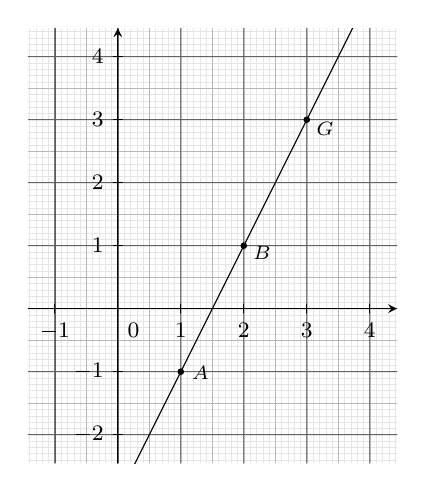
\begin{tikzpicture}[scale = .8 , line cap=round,line join=round,>=stealth,x=1.0cm,y=1.0cm]
		\draw [color=black, xstep=.1,ystep=.1, opacity=.1, line width=.1] (-1.42,-2.45) grid (4.43,4.45);
		\draw [color=black, xstep=.5,ystep=.5, opacity=.2, line width=.2] (-1.42,-2.45) grid (4.43,4.45);
		\draw [color=black, xstep=1,ystep=1, opacity=.5, line width=.5] (-1.42,-2.45) grid (4.43,4.45);
		\draw[->,color=black] (-1.42,0) -- (4.43,0);
		\foreach \x in {-1,1,2,3,4}
		\draw[shift={(\x,0)},color=black] (0pt,2pt) -- (0pt,-2pt) node[below] {\footnotesize $\x$};
		\draw[->,color=black] (0,-2.45) -- (0,4.45);
		\foreach \y in {-2,-1,1,2,3,4}
		\draw[shift={(0,\y)},color=black] (2pt,0pt) -- (-2pt,0pt) node[left] {\footnotesize $\y$};
		\draw[color=black] (0pt,-10pt) node[right] {\footnotesize $0$};
		\clip(-1.42,-2.45) rectangle (4.43,4.45);
		\draw [domain=-1.42:4.43] plot(\x,{(--3-2*\x)/-1});
		\begin{scriptsize}
			\fill [color=black] (1,-1) circle (1.5pt);
			\draw[color=black] (1.31,-1.02) node {$A$};
			\fill [color=black] (2,1) circle (1.5pt);
			\draw[color=black] (2.29,0.88) node {$B$};
			\fill [color=black] (3,3) circle (1.5pt);
			\draw[color=black] (3.29,2.85) node {$G$};
		\end{scriptsize}
	\end{tikzpicture}
\end{minipage}
\end{exe}
%
\subsection{Propri\'et\'es du barycentre pour deux points pond\'er\'es}
\begin{prop}[Colin\'earit\'e]
	Si $G$ est le barycentre du syst\`eme pond\'er\'e non nul $\{ (A,\alpha) , (B,\beta) \}$ 
	alors $G$ appartient \`a la droite $(AB)$.
	
	Si, de plus, $G $ appartient au segment $[AB]$ alors $\alpha et \beta$ sont de m\^eme signe.
%
	\begin{proof}
		Comme $G$ est le barycentre du syst\`eme pond\'er\'e $\{ (A,\alpha) , (B,\beta) \}$, 
		alors $\alpha \overrightarrow{GA} + \beta \overrightarrow{GB} = \vec{0}$
		ce qui nous donne $\alpha \overrightarrow{GA} = -\beta \overrightarrow{GB}$
		ou encore $\overrightarrow{GA} = - \frac{\beta}{\alpha} \overrightarrow{GB}$
		ce qui prouve que $\overrightarrow{GA}$ et $\overrightarrow{GB}$ sont colin\'eaires.
		
		Si, de plus, $G \in [AB]$, alors $\overrightarrow{GA}$ et $\overrightarrow{GB}$ 
		sont de sens oppos\'es ce qui se traduit par le fait que 
		$\overrightarrow{GA} = k \overrightarrow{GB}$ o\`u $k$ est un nombre n\'egatif.
		Comme on sait que $\overrightarrow{GA} = - \frac{\beta}{\alpha} \overrightarrow{GB}$, 
		alors $- \frac{\beta}{\alpha}$ est un nombre n\'egatif ; cela entra\^ine que  
		$\frac{\beta}{\alpha}$ est de signe positif et donc que $\alpha$ et $\beta$ sont de m\^eme signe.
	\end{proof}
\end{prop}
%
\begin{prp}
	Soient $A$ et $B$ deux points distincts et $\D$ la droite $(AB)$.
	\begin{itemize} 
		\item Tout point de $\D$ peut s'\'ecrire comme barycentre des points $A$ et $B$.
		\item Pour un point $M$ de $\D$, il existe plusieurs mani\'eres d'\'ecrire $M$ comme barycentre de $A$ et $B$.
	\end{itemize}
	%
	\begin{proof}
		\begin{itemize} 
		\item Soit $M$ un point de la droite $\D$.
			Comme $A$, $B$ et $M$ sont colin\'eaire, 
			il existe un r\'eel $\mu$ tel que $\overrightarrow{AM} = \mu \overrightarrow{AB}$
			en utilisant la relation de Chasles,
			on a $\overrightarrow{AM} = \mu (\overrightarrow{AM} + \overrightarrow{MB})$
			et donc $ \vec{0} = \mu \overrightarrow{AM} + \mu \overrightarrow{MB} + \overrightarrow{MA} $
			puis $\vec{0} = \overrightarrow{MA} - \mu \overrightarrow{MA} + \mu \overrightarrow{MB}$
			et enfin, $(1-\mu) \overrightarrow{MA} + \mu \overrightarrow{MB} = \vec{0}$.
			Comme $(1-\mu) + \mu = 1 \neq 0$, donc on peut prendre $\alpha = (1-\mu)$ et $\beta = \mu$ ; 
			on a alors $\alpha \overrightarrow{MA} + \beta \overrightarrow{MB} = \vec{0}$ 
			ce qui signifie que $M$ est un barycentre de $A$ et $B$.
		\item Soit maintenant $G$ le barycentre du syst\`eme $\{ (A,\alpha) ; (B,\beta) \}$.
			Cela signifie que $\alpha \overrightarrow{GA} + \beta \overrightarrow{GB} = \vec{0}$.
			Si $\gamma$ est un nombre r\'eel non-nul, 
			alors $\gamma \alpha \overrightarrow{GA} + \gamma \beta \overrightarrow{GB} = \vec{0}$.
			Ainsi, $G$ est aussi le barycentre du syst\'eme $\{ (A,\gamma \alpha) ; (B,\gamma \beta) \}$.
		\end{itemize}
	\end{proof}
\end{prp}
%
Si $M$ est le barycentre du syst\`eme $\{ (A, \alpha) ; (B, \beta) \}$, alors le couple $(\alpha,\beta)$ constitue les \emph{coordonn\'ees barycentriques} de $M$ par rapport \`a $(A,B)$.
%
\subsection{Barycentre de trois points pond\'er\'es}
\index{Barycentre!de trois points}
%
\begin{defi}
Etant donn\'e un syst\`eme de trois points pond\'er\'es $\{ (A, \alpha) ; (B, \beta) ; (C, \gamma) \}$ tel que 
$\alpha + \beta + \gamma \neq 0$,
on appelle barycentre du syst\`eme le point $M$ du plan tel que $\alpha \overrightarrow{MA} + \beta \overrightarrow{MB} + \gamma \overrightarrow{MC} = \vec{0}$.
\end{defi}

Montrons que tout syst\`eme de cette forme admet un barycentre. \\
Notons par $\mathcal{P}$ le plan euclidien et par $\overrightarrow{\mathcal{P}}$ le plan vectoriel.
Soit $\vec{f}$ l'application de $\mathcal{P}$ vers $\overrightarrow{\mathcal{P}}$ qui, \`a tout point $M$ de $\mathcal{P}$,
associe le vecteur $\alpha \overrightarrow{MA} + \beta \overrightarrow{MB} + \gamma \overrightarrow{MC}$.
On veut alors conna\^itre les solutions de l'\'equation $\vec{f}(M) = \vec{0}$.

Prenons un point $N$ de $\mathcal{P}$.
D'apr\`es la relation de Chasles, on a \\
\begin{align*}
\vec{f}(M) & = \alpha \overrightarrow{MN} + \alpha \overrightarrow{NA} + \beta \overrightarrow{MN} + \beta \overrightarrow{NB} + \gamma \overrightarrow{MN} + \gamma \overrightarrow{NC} \\
           & = (\alpha + \beta + \gamma) \overrightarrow{MN} + \vec{f}(N)      \; .
\end{align*}
\begin{itemize} 
\item Si $\alpha + \beta + \gamma = 0$ alors $\vec{f}(M) = \vec{f}(N)$ pour tout $M$ et $N$ de $\mathcal{P}$ et la fonction $\vec{f}$ est donc constante%
\footnote{\'egal \`a $\beta \overrightarrow{AB} + \gamma \overrightarrow{AC}$}.
\item Si $\alpha + \beta + \gamma \neq 0$, fixons un origine qu'on appellera $O$.
      On a alors
      \begin{align*}
      \vec{f}(G) & = (\alpha + \beta + \gamma) \overrightarrow{GO} + \overrightarrow{f(O)} \\
                 & = (\alpha + \beta + \gamma) \overrightarrow{GO} + \alpha \overrightarrow{OA} + \beta \overrightarrow{OB} + \gamma \overrightarrow{OC} \\
      \intertext{et si $G$ est le barycentre alors $\vec{f}(G) = \vec{0}$ et on a }
      \vec{0} & = (\alpha + \beta + \gamma) \overrightarrow{GO} + \alpha \overrightarrow{OA} + \beta \overrightarrow{OB} + \gamma \overrightarrow{OC} \\
      \intertext{et ainsi}
      \end{align*}
\propbox{$$\overrightarrow{OG} = \frac{ \alpha \overrightarrow{OA} + \beta \overrightarrow{OB} + \gamma \overrightarrow{OC} }{ \alpha + \beta + \gamma } \; .$$}
\end{itemize}
%
\begin{thm}
Si $\alpha + \beta + \gamma \neq 0$, alors il existe un unique point $G$ tel que $\alpha \overrightarrow{GA} + \beta \overrightarrow{GB} + \gamma \overrightarrow{GC} = \vec{0}$.
Ce point $G$ est appel\'e \emph{barycentre} du syst\`eme $((A,\alpha),(B,\beta),(C,\gamma))$.
\end{thm}
%
\subsubsection{Coordonn\'ees du barycentre}
On rapporte maintenant le plan $\mathcal{P}$ \`a un rep\`ere $(O,\vec{\imath},\vec{\jmath})$.
Soit $((A,\alpha),(B,\beta),(C,\gamma))$ un syst\`eme de points pond\'er\'es tel que $\alpha + \beta + \gamma \neq 0$.
Soient $(x_A , y_A)$, $(x_B , y_B)$ et $(x_C , y_C)$ les coordonn\'ees respectives de $A$, $B$ et $C$.
Soit $G (x_G , y_G)$ le barycentre du syst\`eme.
Comme $\overrightarrow{OG} = \frac{\alpha \overrightarrow{OA} + \beta \overrightarrow{OB} + \gamma \overrightarrow{OC}}{\alpha + \beta + \gamma}$, on a 
\[
\left\lbrace
\begin{matrix}
x_G = \frac{\alpha x_A + \beta x_B + \gamma x_C }{\alpha + \beta + \gamma} \\
y_G = \frac{\alpha y_A + \beta y_B + \gamma y_C }{\alpha + \beta + \gamma} \; .
\end{matrix}
\right.
\]
Tout triplet $(\alpha , \beta , \gamma)$ tel que $M$ soit un barycentre de $((A,\alpha),(B,\beta),(C,\gamma))$ constitue des \emph{coordonn\'ees barycentriques}.
%
\subsubsection{Associativit\'e du barycentre}
\index{Barycentre!associativite@associativit\'e}
Soient les deux syst\`emes de points pond\'er\'es non nuls
\[
  \begin{aligned}
    \mathcal{S}  &= ((A,\alpha),(B,\beta),(C,\gamma)), \\
    \mathcal{S}' &= ((A,\alpha),(B,\beta)).
  \end{aligned}
\]
On note $G$ le barycentre de $\mathcal{S}$ et $G'$ celui de $\mathcal{S}'$.
\par\noindent
\propbox{Alors $G$ est aussi le barycentre du syst\`eme
$\left((G',\alpha+\beta),(C,\gamma)\right)$.}
%
\begin{proof}
En effet, avec ces hypoth\`eses on a $\alpha \overrightarrow{G' A} + \beta \overrightarrow{G' B} = \vec{0}$ ce qui, d'apr\`es la relation de Chasles, donne 
$\alpha \overrightarrow{GA} + \beta \overrightarrow{GB} = (\alpha + \beta) \overrightarrow{GG'}$.
Combinant cette derni\`ere avec l'\'egalit\'e $\alpha \overrightarrow{GA} + \beta \overrightarrow{GB} + \gamma \overrightarrow{GC} = \vec{0}$, on a 
$(\alpha + \beta) \overrightarrow{GG'} + \gamma \overrightarrow{GC} = \vec{0}$ ce qui montre que $G$ est le barycentre du syst\`eme $((G' , \alpha + \beta),(C , \gamma))$.
\end{proof}
%
\subsection{Barycentre de $n$ points pond\'er\'es}
\index{Barycentre!de n points@de $n$ points}
%
Le barycentre de $n$ points pond\'er\'es n'est autre qu'une g\'en\'eralisation du barycentre de trois points pond\'er\'es.
      \begin{defi}
            Soient $A_1,\ A_2,\ \ldots ,\ A_n$ $n$ points distincts du plan.
            Soient $\alpha_1,\ \alpha_2,\ \ldots ,\ \alpha_n$ $n$ nombres r\'eels.
            
            Si $\alpha_1 + \alpha_2 + \cdots + \alpha_n \neq 0$ alors il existe un unique point $G$ 
            tel que $\alpha_1 \overrightarrow{GA_1} + \alpha_2 \overrightarrow{GA_2} + \cdots + \alpha_n \overrightarrow{GA_n} = \vec{0}$.
            
	            Le point $G$ ainsi d\'efini est appel\'e \emph{barycentre} du syst\`eme 
	            \[
	              \left\lbrace (A_1,\alpha_1) ; (A_2,\alpha_2) ; \ldots ; (A_n,\alpha_n) \right\rbrace.
	            \]
      \end{defi}
      %
      \begin{prop}
            Soient 
            $\left\lbrace (A_1,\alpha_1) ; (A_2,\alpha_2) ; \ldots ; (A_n,\alpha_n) \right\rbrace$
            un syst\`eme de points pond\'er\'es v\'erifiant $\sum \alpha_i \neq 0$ et soit $G$ le barycentre de ce syst\`eme.
            
            \begin{enumerate}
                  \item le barycentre $G$ est ind\'ependant de l'ordre des couples $(A_i , \alpha_i)$,
	                  \item pour tout r\'eel non nul $k$, le point $G$ est aussi le barycentre du syst\`eme 
	                        \[
	                          \left\lbrace (A_1,k\alpha_1) ; (A_2,k\alpha_2) ; \ldots ; (A_n,k\alpha_n) \right\rbrace,
	                        \]
                  \item \index{Barycentre!isobarycentre}
\index{centre de gravite@centre de gravit\'e}
                        si $\alpha_1 = \alpha_2 = \cdots = \alpha_n$, on dit que $G$ est 
                        l'\emph{isobarycentre} ou le centre de gravit\'e des points 
                        $A_1,\ A_2,\ \ldots ,\ A_n$,
                  \item \label{prop: associativite}
                        si $p<n$ et que $\alpha_1 + \alpha_2 + \cdots + \alpha_p = \alpha' \neq 0$, alors 
	                        le syst\`eme 
	                        \[
	                          \left\lbrace (A_1,\alpha_1) ; (A_2,\alpha_2) ; \ldots ; (A_p,\alpha_p) \right\rbrace
	                        \]
                        admet un barycentre $G'$.
	                        Le point $G$ est aussi le barycentre du syst\`eme 
	                        \[
	                          \left\lbrace (G',\alpha') ; (A_{p+1},\alpha_{p+1}) , \ldots , (A_n,\alpha_n) \right\rbrace.
	                        \]
            \end{enumerate}
            %
            \smallnota{Comme l'ordre des couples ne change pas le barycentre,
                       le point $G'$ de \ref{prop: associativite} peut \^etre remplac\'e par
                       le barycentre de n'importe quel sous-ensemble de $p$ couples, 
                       et non seulement des $p$ premiers.
                       }
      \end{prop}
%
\section{Fonctions de Leibniz}
%
\subsection{Fonction vectorielle de Leibniz}
\index{Leibniz!Fonction vectorielle de}
%
On consid\`ere l'espace affine $E$ associ\'e \`a l'espace vectoriel $V$. 
Soit $(A_i , \alpha_i)_{i = 1 , \dots , n}$ une famille de points pond\'er\'es.
\begin{defi} ~ \newline
On appelle \emph{fonction vectorielle de Leibniz} associ\'ee au syst\`eme
$\{(A_i,\alpha_i)\}_{i=1,\dots,n}$ l'application de $E$ dans $V$ qui, \`a tout point $M$, associe le vecteur
	\defbox{
		$$
			\vec{f}(M) = \sum_{i = 1}^{n} \alpha_i \overrightarrow{MA_i}
			\; .
		$$
	}
\end{defi}
%
Posons $m = \sum_{i = 1}^{n} \alpha_i$.
%
\begin{prp}
	\label{prp:f(M) = f(N) + m MN}
	Pour tout couple de points $(M , N)$, on a 
		\propbox{
			$$   \vec{f}(M) = \vec{f}(N) + m \; \overrightarrow{MN}		\; .$$
		}
	%
	\begin{proof}
		Soit $(M,N)$ un couple de points de $E$.
		D'apr\`es la relation de Chasles, on a 
			\begin{displaymath}
			\vec{f}(M) = \sum_{i = 1}^n \alpha_i ( \overrightarrow{MN} + \overrightarrow{NA_i} ) 
				= \sum_{i = 1}^n \alpha_i  \overrightarrow{MN} + \sum_{i = 1}^n \alpha_i \overrightarrow{NA_i} 
				= \left( \sum_{i = 1}^n \alpha_i \right) \cdot \overrightarrow{MN} + \vec{f}(N)           
			\; .
			\end{displaymath}
	\end{proof}
\end{prp}
%
\begin{prp} \label{prp:fonction vectorielle}
	Selon la valeur de $\sum_{i = 1}^{n} \alpha_i$, on distingue deux cas : 
	\begin{enumerate}
	\item \textbf{Si $\mathbold{\sum_{i = 1}^{n} \alpha_i = 0}$ } alors la fonction $\vec{f}$ est constante.
	\item \label{prp: fonction vectorielle 2}
		\textbf{Si $\mathbold{\sum_{i = 1}^{n} \alpha_i \neq 0}$ } alors il existe un point $G$ tel que $\vec{f}(G) = \vec{0}$. De plus, pour tout point $M$ on a $\vec{f}(M) = (\sum_{i = 1}^{n} \alpha_i) \; \overrightarrow{MG}$.
	\end{enumerate}
	\begin{proof}
		\begin{enumerate}
			\item Supposons que $\sum_{i = 1}^{n} \alpha_i = 0$. 
				Soient $M$ et $N$ deux points.
				D'apr\`es la Propri\'et\'e~\ref{prp:f(M) = f(N) + m MN}, 
				on a $\vec{f}(M) = \vec{f}(N) + m \; \overrightarrow{MN}$.
				Comme $m = 0$ alors $\vec{f}(M) = \vec{f}(N)$.
				On d\'eduit que $\vec{f}$ est constante.
			\item Supposons que $\sum_{i = 1}^{n} \alpha_i \neq 0$. 
				Fixons un point $O$ comme origine. 
				D'apr\`es la Propri\'et\'e~\ref{prp:f(M) = f(N) + m MN}, 
				pour tout point $M$ on a $\vec{f}(M) = \overrightarrow{f(O)} + m \; \overrightarrow{MO}$.
				Cette propri\'et\'e est en particulier vraie pour le point $G$ tel que
				$\overrightarrow{OG} = \frac{1}{m} \; \overrightarrow{f(O)}$.
				On obtient alors 
				\begin{align*}
					\vec{f}(G) & = \overrightarrow{f(O)} + m \;\overrightarrow{GO}                 
						  = \overrightarrow{f(O)} - m \;\overrightarrow{OG}                         \\
						& = \overrightarrow{f(O)} - m \; \frac{1}{m} \; \overrightarrow{f(O)}       
						  = \overrightarrow{f(O)} - \overrightarrow{f(O)}                           
						  = \vec{0}                                           .
				\end{align*}
				Soit $M$ un point de $E$.
				En appliquant la Propri\'et\'e~\ref{prp:f(M) = f(N) + m MN} au points $M$ et $G$, on obtient 
				$$
					\vec{f}(M) = \vec{f}(G) + m \; \overrightarrow{MG} 
							\text{ et comme $\vec{f}(G) = \vec{0}$ alors } \vec{f}(M) 
						= m \; \overrightarrow{MG} 
					\; .
				$$
		\end{enumerate}
	\end{proof}
\end{prp}
%
\nota{
La premi\`ere partie de la Propri\'et\'e~\ref{prp:fonction vectorielle}~\ref{prp: fonction vectorielle 2} m\'erite une attention particuli\`ere.
La voici donc r\'ep\'et\'ee, cette fois, avec l'honneur qui lui est d\^u.
		\thmbox{
			Si $\sum_{i = 1}^{n} \alpha _{i} \neq 0$, alors il existe un point $G$ tel que $\vec{f}(G) = \vec{0}$.
		}
}
%
\subsection{Fonction scalaire de Leibniz}
\index{Leibniz!Fonction scalaire de}
%
On consid\`ere l'espace affine $E$ associ\'e \`a l'espace vectoriel $V$. 
Soit $(A_i , \alpha_i)_{i = 1 , \dots , n}$ une famille de points pond\'er\'es.
\begin{defi}
On appelle \emph{fonction scalaire de Leibniz} associ\'ee au syst\`eme
$\{(A_i,\alpha_i)\}_{i=1,\dots,n}$ l'application de $E$ dans $\mathbb{R}$ qui, \`a tout point $M$, associe le r\'eel
      \defbox{
	      $$
		      \varphi (M) = \sum_{i = 1}^n \alpha_i \; {\overrightarrow{M A_i}}^{2}
		      \; .
	      $$
      }      
\end{defi}
%
Posons $m = \sum_{i = 1}^n \alpha_i$.
%
\begin{prp} \label{prp: fonction scalaire}
\begin{enumerate}
\item \label{prp: fonction scalaire 1}
      Pour tout points $M$ et $N$, on a :
      $\displaystyle{
      \varphi(M) = m \; {\overrightarrow{MN}}^2 
                 + 2 \; \overrightarrow{MN} \cdot \vec{f}(N)
                 + \varphi(N)
      \; .
      }$
\item Si $\sum_{i = 1}^n \alpha_i = 0$ alors 
      $\displaystyle{
      \varphi (M) = 2 \; \overrightarrow{MN} \cdot \sum_{i = 1}^n \alpha_i \overrightarrow{N A_i} + \varphi(N)
      \; .
      }$
\item Si $\sum_{i = 1}^n \alpha_i \neq 0$ alors le syst\`eme $\left\{ \left( A_i , \alpha_i \right) \mid 1 \leq i \leq n \right\}$
      admet un barycentre $G$ ; et on a pour tout point $M$       
      $\displaystyle{
      \varphi(M) = m \; {\overrightarrow{MG}}^2 + \varphi(G)
      \; .
      }$
\end{enumerate}
\begin{proof}
\begin{enumerate}
\item Soient $M$ et $N$ deux points.
      $\displaystyle{\varphi(M) = \sum_{i = 1}^n \alpha_i \; {\overrightarrow{M A_i}}^2}$
      d'apr\`es la relation de Chasles, on a 
      \begin{align*}
      \varphi(M) 
                 & = \sum_{i = 1}^n \alpha_i \; \left( \overrightarrow{MN} + \overrightarrow{N A_i} \right)^2 
                   = \sum_{i = 1}^n \alpha_i \; \left( {\overrightarrow{MN}}^2 + 2 \; \overrightarrow{MN} \cdot \overrightarrow{NA_i} + {\overrightarrow{N A_i}}^2 \right) \\
                 & = \sum_{i = 1}^n \alpha_i \; {\overrightarrow{MN}}^2
                   + \sum_{i = 1}^n \alpha_i \; 2 \; \overrightarrow{MN} \cdot \overrightarrow{NA_i}
                   + \sum_{i = 1}^n \alpha_i \; {\overrightarrow{N A_i}}^2 \\
                 & = m \; {\overrightarrow{MN}}^2 + 2 \; \overrightarrow{MN} \cdot \vec{f}(N) + \varphi(N) \;.
      \end{align*}
\item Il suffit d'appliquer la propri\'et\'e pr\'ec\'edente au cas $m = 0$.      
\item Il suffit d'appliquer la Propri\'et\'e~\ref{prp: fonction scalaire}~\ref{prp: fonction scalaire 1} \`a $G$, en remarquant que $\vec{f}(G) = \vec{0}$.
\end{enumerate}
\end{proof}
\end{prp}
%
\subsection{Lignes de niveau}
\index{Ligne de niveau}
%
Soient $(A_i , \alpha_i)_{1\leq i\leq n}$ un syst\`eme de points pond\'er\'es et $\varphi$ la fonction scalaire de Leibniz associ\'ee.
On appelle \emph{ligne de niveau $k$} de $\varphi$ l'ensemble des points $M$ tels que $\varphi(M) = k$.
En utilisant la Propri\'et\'e~\ref{prp: fonction scalaire}~\ref{prp: fonction scalaire 1}, on obtient pour tout bipoints $(M,N)$ :
\begin{displaymath}
\varphi(M) = m \; {\overrightarrow{MN}}^2 + 2 \; \overrightarrow{MN} \cdot \vec{f}(N) + \varphi(N)
\end{displaymath}
et on distingue alors deux cas suivant la valeur de $m$.
\begin{enumerate}
\item \textbf{Si $\mathbf{m = 0}$ }
      alors, comme $\vec{f}$ est constante, \'egal \`a un vecteur qu'on notera $\vec{v}$, on obtient: 
      $$
      \varphi (M) = 2 \; {\overrightarrow{MN}} \cdot \vec{v} + \varphi (N)
      \; .
      $$
      
      Dans ce cas, si on conna\^it un point $A$ appartenant \`a la ligne de niveau $k$ (c'est-\`a-dire tel que $\varphi (A) = k$),
      alors on obtient 
      $
      \varphi (M) = 2 \; \overrightarrow{MA} \cdot \vec{v} + k
      $
      et l'ensemble des points $M$ tels que $\varphi (M) = k$ n'est autre que l'ensemble des points $M$ tels que 
      $\overrightarrow{MA} \cdot \vec{v} = 0$ (ce qui est possible seulement quand $\overrightarrow{MA} \perp \vec{v}$). 
      Autrement dit, la ligne de niveau $k$ est la 
      \propbox{droite passant par $A$ et de direction perpendiculaire \`a $\vec{v}$}.
      
\item \textbf{Si $\mathbf{m \neq 0}$ }
      alors, le syst\`eme $(A_i , \alpha_i)_{1\leq i\leq n}$ admet un barycentre $G$ ; on obtient alors : 
      $$
      \varphi (M) = m \; {\overrightarrow{MG}}^2 + \varphi (G)
      \; .
      $$ 
      Dans ce cas, l'\'equation $\varphi (M) = k$ \'equivaut \`a $ m \; {\overrightarrow{MG}}^2 + \varphi (G) = k$ et donc 
      \begin{equation} \label{eq: ligne de niveau m neq 0}
      {\overrightarrow{MG}}^2 = \frac{k - \varphi (G)}{m}      
      \; 
      \end{equation}
      Posons $a = \frac{k - \varphi (G)}{m}$.
      On distingue alors 3 cas suivant les valeurs de $a$.
      \begin{itemize} 
      \item \textbf{Si $\mathbf{a < 0}$ :} 
            alors l'\'Equation \eqref{eq: ligne de niveau m neq 0} n'admet pas de solution et 
            la ligne de niveau est \propbox{$\emptyset$}.
      \item \textbf{Si $\mathbf{a = 0}$ :} 
            alors l'\'Equation \eqref{eq: ligne de niveau m neq 0} admet une solution unique $G$.
            La ligne de niveau $k$ est donc \propbox{$\{ G \}$}.
      \item \textbf{Si $\mathbf{a > 0}$ :} 
            alors $MG = \sqrt{a} $.
            Ainsi, la ligne de niveau $k$ est l'ensemble des points $M$ tels que 
            la distance entre $M$ et $G$ est \'egale \`a $\sqrt{a}$.
            Autrement dit, c'est le
            \propbox{cercle de centre $G$ et de rayon $\sqrt{a}$}.
      \end{itemize}
\end{enumerate}


























\end{chapter}

\TCDLessonStyleOff
\clearpage
\providecommand{\Plan}{(\mathscr{P})}
\providecommand{\mes}[2]{\mathrm{mes}\left( \widehat{ \overrightarrow{#1} , \overrightarrow{#2} } \right)}
\section{Exercices}
\begin{exo}
      Soit $ABC$ un triangle rectangle direct en $A$ tel que $AB = 2AC$. 
      Pour chacune des questions suivantes, d\'eterminer et construire le barycentre $G$ du syst\`eme $[(A,\alpha) ; (B,\beta) ; (C,\gamma) ]$.
      \begin{enumerate}
            \item $(\alpha , \beta , \gamma) = (1,-2,3)$,
            \item $(\alpha , \beta , \gamma) = (-1,-1,3)$,
            \item $(\alpha , \beta , \gamma) = (1,-1,2)$,
            \item $(\alpha , \beta , \gamma) = (\frac{1}{2},-1,1)$.
      \end{enumerate}
\end{exo}
%
\begin{exo}
      Soient $A$, $B$ et $C$ trois points du plan affine euclidien.
      D\'eterminer les coefficients $a$ et $b$ pour que le point $C$ soit le barycentre du syst\`eme $[(A,a);(B,b)]$.
      \begin{enumerate}
            \item $\overrightarrow{AC} = \frac{2}{3} \overrightarrow{BA}$,
            \item $4\overrightarrow{BC} + \frac{2}{3} \overrightarrow{BA} = \overrightarrow{0}$,
            \item $2 \overrightarrow{AC} - 5 \overrightarrow{BA} = \overrightarrow{0}$.
      \end{enumerate}
\end{exo}
%
\begin{exo}
      Soit $ABC$ un triangle quelconque.
      \begin{enumerate}
            \item Construire les points $I$, $J$ et $K$ ; milieux respectifs de $[BC]$, $[CA]$ et $[AB]$.
            \item Construire le point $G$, isobarycentre des points $A$, $B$ et $C$.
            \item D\'emontrer que les droites $(AI)$, $(BJ)$ et $(CK)$ son concourantes au point $G$.
      \end{enumerate}
\end{exo}
%
\begin{exo}
      Soient $A$, $B$, $C$ et $D$ quatre points du plan affine r\'eel $\mathcal{E}$.
      On d\'esigne par $I$ et $J$ les milieux respectifs de $[AB]$ et $[CD]$.
      Soit $G$ le barycentre de $(I,\alpha)$ et $(J,\beta)$ avec $\alpha + \beta \neq 0$.
      \begin{enumerate}
            \item D\'emontrer que $G$ est le barycentre de $[(A,\alpha) ; (B,\alpha) ; (C,\beta) ; (D,\beta)]$.
                  En d\'eduire l'expression du vecteur 
                  $\alpha \left( \overrightarrow{MA} + \overrightarrow{MB} \right) + \beta \left( \overrightarrow{MC} + \overrightarrow{MD} \right)$
                  en fonction de $\alpha$, $\beta$ et $\overrightarrow{MG}$, $M$ \'etant un point quelconque du plan.
            \item $\vec{u}$ \'etant un vecteur du plan vectoriel $\overrightarrow{E}$ associ\'e \`a $\mathcal{E}$,
                  quel est l'ensemble des points $M$ tels que les vecteurs $\overrightarrow{u}$ et
                  $\alpha \left( \overrightarrow{MA} + \overrightarrow{MB} \right) + \beta \left( \overrightarrow{MC} + \overrightarrow{MD} \right)$
                  soient lin\'eairement d\'ependant\,?
      \end{enumerate}
\end{exo}
%
\begin{exo}
      On donne un triangle $ABC$.
      $\alpha$ et $\beta$ sont deux nombres r\'eels tels que $\alpha + \beta \neq 0$.
      Soient $C'$ le barycentre de $(A,\alpha)$ et $(B,\beta)$,
      $B'$ le barycentre de $(A,\beta)$ et $(C,\alpha)$ et 
      $G$ l'isobarycentre de $A$, $B'$ et $C'$.
      \begin{enumerate}
            \item Exprimer $\overrightarrow{AC'}$, $\overrightarrow{AB'}$ et $\overrightarrow{AG}$ en fonction de $\alpha$, $\beta$, $\overrightarrow{AB}$ et $\overrightarrow{AC}$.
            \item D\'eterminer l'ensemble des points $G$ lorsque $\alpha$ et $\beta$ 
                  varient de fa\c{c}on que $\alpha + \beta = 1$. (On pourra utiliser le rep\`ere $(A,\overrightarrow{AB},\overrightarrow{AC})$.)
            \item Retrouver ce r\'esultat en utilisant les points $B_1$ et $C_1$ d\'efinis par : 
                  $3\overrightarrow{AB_1} = \overrightarrow{AB}$ et $3\overrightarrow{AC_1} = \overrightarrow{AC}$.
      \end{enumerate}
\end{exo}
%
\begin{exo}
      Dans le plan affine euclidien, on consid\`ere trois points $A$, $B$ et $C$ non align\'es.
      Soit $M$ un point quelconque du plan.
            \begin{enumerate}
                  \item Montrer que le vecteur $\vec{v}_M = 2 \overrightarrow{MA} + \overrightarrow{MB} - 3 \overrightarrow{MC}$
                        est \'egal \`a un vecteur $\vec{v}$ ind\'ependant de $M$.
                  \item Soit $P$ le point tel que $\overrightarrow{AP} = \vec{v}$.
                        La droite $(AP)$ coupe la droite $(BC)$ en un point $U$.
                        D\'emontrer que $\overrightarrow{UB} = 3 \overrightarrow{UC}$.
                        Comparer $\overrightarrow{UP}$ et $\overrightarrow{UA}$ puis $\overrightarrow{PB}$ et $\overrightarrow{AC}$.
                  \item Soit $O$ le centre du cercle circonscrit au triangle $ABC$.
                        \`Etablir la relation : $2 MA^2 + MB^2 - 3 MC^2 = 2 \overrightarrow{MO} \cdot \vec{v}$.
                        En d\'eduire l'ensemble des points $M$ tels que : $2 MA^2 + MB^2 - 3 MC^2 = 0$.
            \end{enumerate}
\end{exo}
%
\begin{exo}
      Dans le plan affine euclidien, on consid\`ere un triangle $ABC$.
      Soit $G$ le barycentre du syst\`eme $[(A,1) ; (B,2) ; (C,-1)]$.
      \`A tout point $M$ du plan, on associe les vecteurs 
            $\vec{u}_{\!\!M} = \overrightarrow{MA} + 2 \overrightarrow{MB} - \overrightarrow{MC}$ et
            $\vec{v} = 2 \overrightarrow{MA} - \overrightarrow{MB} - \overrightarrow{MC}$.
            \begin{enumerate}
                  \item D\'eterminer et construire le point $G$.
                  \item D\'eterminer l'ensemble $D$ des points $M$ pour lesquels 
                        $\vec{u}_M$ et $\vec{v}$ sont lin\'eairement d\'ependants.
                  \item D\'eterminer l'ensemble $\Delta$ des points $M$ pour lesquels $\vec{u}_{\!\!M} \cdot \vec{v} = 0$.
                  \item D\'eterminer l'ensemble $\Gamma$ des points $M$ pour lesquels $\| \vec{u}_{\!\!M} \| = \| \vec{v} \|$.
            \end{enumerate}
\end{exo}
%
\begin{exo}
      Soit, dans le plan affine euclidien un carr\'e $ABCD$.
      \begin{enumerate}
            \item D\'eterminer un syst\`eme de coordonn\'ees barycentriques de $A$ dans le rep\`ere affine $(B,C,D)$.
            \item D\'eterminer l'ensemble des points $M$ tels que : 
                  $\overrightarrow{MC} \cdot \overrightarrow{MB} + \overrightarrow{MC} \cdot \overrightarrow{MD} - MC^2 = 0$.
      \end{enumerate}
\end{exo}
%
\begin{exo}
      On se place dans le plan affine euclidien.
      Soit $a$ un nombre r\'eel positif.
      On consid\`ere le triangle $ABC$ tel que : $AB = 3a$, $AC = 4a$ et $BC = 5a$.
      \begin{enumerate}
            \item D\'eterminer le barycentre $G$ des points $A$, $B$ et $C$ 
                  affect\'es respectivement des coefficients $-5$, $4$ et $3$.
            \item Calculer $GA$ ,$GB$ et $GC$ en fonction de $a$.
            \item Etant donn\'e un nombre r\'eel $k$, d\'eterminer l'ensemble des points $M$ du plan tel que
                  $4 MB^2 + 3 MC^2 - 5 MA^2 = k a^2$.
      \end{enumerate}
\end{exo}
%
\begin{exo}
      Soit $ABC$ un triangle rectangle isoc\`ele en $A$ tel que 
      $AB = AC = a$ o\`u $a$ est un r\'eel strictement positif.
      On appelle $\varphi$ et $\psi$ les applications du plan dans $\mathbb{R}$ qui, 
      \`a tout point $M$ du plan, associe respectivement les r\'eels 
      $\varphi (M) = MA^2 - MB^2 - MC^2$ et $\psi (M) = MA^2 + MB^2 - 2 MC^2$.
      On note $G$ le barycentre du syst\`eme $[(A,1) ; (B,-1) ; (C,-1)]$.
      \begin{enumerate}
            \item Exprimer $\varphi (M)$ en fonction de $MG$.
            \item V\'erifier que $\psi (M) - \psi (A) = 2 \overrightarrow{MA} (\overrightarrow{AB} - 2 \overrightarrow{AC})$.
            \item D\'eterminer l'ensemble $\Sigma$ des points $M$ du plan tels que $\varphi (M) = -a^2$.
            \item D\'eterminer l'ensemble $D$ des points $M$ du plan tels que $\psi (M) = \psi (A)$.
      \end{enumerate}
\end{exo}
%%%%%%%%%%%%%%%%%% MBA ATAOVY ALOHA ITO IZAY VAO OMENA MPIANATRA %%%%%%%%%%%%%%%%%% 
%\begin{exo}
%      Dans le plan $\Plan$ on consid\`ere le triangle \'equilat\'eral $ABC$.
%      On pose $AB = BC = CA = a$, $a>0$.
%      \begin{enumerate}
%            \item Construire le point $G$ barycentre du syst\`eme $\{(A,2),(B,1),(C,1)\}$.
%            \item D\'eterminer et construire chacun des deux ensembles suivants : 
%                  \begin{enumerate}
%                        \item \[
%                                    E_1 = \left\lbrace M \in \Plan \middle| 2 MA^2 + MB^2 + MC^2 = 2 a^2 \right\rbrace \;.
%                              \]
%                        \item \[
%                                    E_2 = \left\lbrace M \in \Plan \middle| 
%                                          2 \overrightarrow{MA}^2 
%                                                + \overrightarrow{MA}\cdot\overrightarrow{MB} 
%                                                      + \overrightarrow{MA}\cdot\overrightarrow{MC} 
%                                                            = \frac{3a^2}{2} \right\rbrace \;.
%                              \]
%                              Pour ce dernier ensemble, on pourra utiliser le point $G$ 
%                              puis le milieu $I$ du segment $[AG]$.
%                  \end{enumerate}
%      \end{enumerate}
%\end{exo}




















% T12 C/D, chapitre 6 : Applications affines et isométries. Source : le livre « Terminales scientifiques » (Affine/Lesona, Isometrie/Lesona, Isometrie/Exo).
% Les exercices tirés d’autres ouvrages ne sont pas repris (décision du 2 novembre 2026).

\TCDLessonStyleOn
\providecommand{\Plan}{\mathscr{P}}
\providecommand{\Espace}{\mathcal{E}}
\providecommand{\bary}[1]{\mathrm{Bar}\left\lbrace #1 \right\rbrace}
\providecommand{\Id}{\mathrm{Id}}
\chapter{Applications affine}
      Dans ce chapitre, $\Plan$ d\'esigne le plan affine et $\Espace$ l'espace affine.
      \section{D\'efinitions et exemples}
            \begin{defi}
\index{Application affine}
                  Une application $f : \Plan \rightarrow \Plan$ est une \emph{application affine}
                  si elle conserve le barycentre.
                  
                  Si $G = \bary{(A,\alpha) ; (B,\beta)}$.
                  En posant $G' = f(G)$, $A' = f(A)$ et $B' = f(B)$, on a 
                  $G' = \bary{(A',\alpha) ; (B',\beta)}$.
            \end{defi}
            %
            \begin{ex}
                  \begin{enumerate}
                        \item Consid\'erons la translation $t_{\vec{u}}$ de vecteur $\vec{u}$.
                              En posant $t_{\vec{u}} (M) = M'$, on a $\overrightarrow{MM'} = \vec{u}$.
                              
                              Soit $G = \bary{(A,\alpha) ; (B,\beta)}$.
                              Soient
                              $G' = t_{\vec{u}} (G)$,
                              $A' = t_{\vec{u}} (A)$ et
                              $B' = t_{\vec{u}} (B)$
                              .
                              On a alors
                              \begin{align*}
                              \alpha \overrightarrow{G'A'} + \beta \overrightarrow{G'B'}
                                    & =  \alpha (\overrightarrow{G'G} + \overrightarrow{GA} + \overrightarrow{AA'})
                                        +\beta (\overrightarrow{G'G} + \overrightarrow{GB} + \overrightarrow{BB'})      \\
                                    & =  \alpha (-\vec{u} + \overrightarrow{GA} + \vec{u})
                                        +\beta (-\vec{u} + \overrightarrow{GB} + \vec{u})      \\
                                    & = \alpha \overrightarrow{GA} + \beta \overrightarrow{GB}      \\
                                    & = \vec{0}.
                              \end{align*}
                              Donc $G' = \bary{(A';\alpha);(B';\beta)}$ et ainsi, $t_{\vec{u}}$ est une application affine.
                  \end{enumerate}
            \end{ex}
            %
            \begin{ex}
                  Consid\'erons l'homoth\'etie $h$ de centre $I$ et de rapport $k$.
                  En posant $h(M) = M'$, on a $\overrightarrow{IM'} = k \overrightarrow{IM}$.
                  
                  On veut montrer que $h$ est une application affine.
                  Consid\'erons le point
                  \[
                  G = \bary{(A,\alpha);(B,\beta)}.
                  \]
                  Posons $G' = h(G)$, $A' = h(A)$ et $B' = h(B)$.
                  On a alors 
                  \begin{align*}
                        \alpha \overrightarrow{G'A'} + \beta \overrightarrow{G'B'}
                              & =  \alpha (\overrightarrow{G'I} + \overrightarrow{IA'})
                                  +\beta (\overrightarrow{G'I} + \overrightarrow{IB'})      \\
                              & = \alpha (k \overrightarrow{GI} + k \overrightarrow{IA}) 
                                  +\beta (k \overrightarrow{GI} + k \overrightarrow{IB})      \\
                              & = k \left[ \alpha \overrightarrow{GA} + \beta \overrightarrow{GB} \right]       
                                = k \vec{0}      
                                = \vec{0}.
                  \end{align*}
            \end{ex}
            %
            \begin{ex}
                  Consid\'erons la r\'eflexion d'axe $(\mathscr{D})$.
                  On veut montrer que la r\'eflexion est une application affine.
                  
                        \begin{tikzpicture}[line cap=round,line join=round,>=triangle 45,x=2.0cm,y=2.0cm]
                              \clip(-0.94,-0.73) rectangle (2.88,2.42);
                              \draw[fill=black,fill opacity=0.1] 
                                    (0.8,1.4) -- (0.81,1.19) -- (1.03,1.19) -- (1.02,1.41) -- cycle; 
                              \draw[fill=black,fill opacity=0.1] 
                                    (0.82,0.7) -- (0.83,0.49) -- (1.05,0.49) -- (1.04,0.71) -- cycle; 
                              \draw[fill=black,fill opacity=0.1] 
                                    (0.85,-0.14) -- (0.85,-0.36) -- (1.07,-0.35) -- (1.06,-0.14) -- cycle; 
                              \draw [domain=-0.94:2.88] plot(\x,{(--1.91-1.8*\x)/0.05});
                              \draw (0.42,-0.15)-- (0,0.68);
                              \draw [dash pattern=on 1pt off 1pt] (0,0.68)-- (-0.36,1.37);
                              \draw (1.7,-0.12)-- (2.08,0.74);
                              \draw [dash pattern=on 1pt off 1pt] (2.08,0.74)-- (2.4,1.45);
                              \draw [dotted] (-0.36,1.37)-- (1.02,1.41);
                              \draw [] (0.33,1.44) -- (0.33,1.35);
                              \draw [dotted] (1.02,1.41)-- (2.4,1.45);
                              \draw [] (1.71,1.48) -- (1.71,1.38);
                              \draw [dotted] (2.08,0.74)-- (1.04,0.71);
                              \draw [] (1.58,0.68) -- (1.58,0.77);
                              \draw [] (1.54,0.68) -- (1.54,0.77);
                              \draw [dotted] (0,0.68)-- (1.04,0.71);
                              \draw [] (0.5,0.74) -- (0.5,0.65);
                              \draw [] (0.53,0.74) -- (0.54,0.65);
                              \draw [dotted] (1.06,-0.14)-- (0.42,-0.15);
                              \draw [] (0.78,-0.19) -- (0.78,-0.1);
                              \draw [] (0.75,-0.19) -- (0.74,-0.1);
                              \draw [] (0.71,-0.19) -- (0.71,-0.1);
                              \draw [dotted] (1.7,-0.12)-- (1.06,-0.14);
                              \draw [] (1.42,-0.17) -- (1.42,-0.08);
                              \draw [] (1.39,-0.17) -- (1.38,-0.08);
                              \draw [] (1.35,-0.17) -- (1.35,-0.08);
                              \draw (1.2,2.24) node[anchor=north west] {$ (\mathscr{D}) $};
                              \begin{scriptsize}
                              \fill [color=black] (0.42,-0.15) circle (1.5pt) node[below left] {$A$};
                              \fill [color=black] (0,0.68) circle (1.5pt) node[below left] {$B$};
                              \fill [color=black] (-0.36,1.37) circle (1.5pt) node[below left] {$G$};
                              \fill [color=black] (1.7,-0.12) circle (1.5pt) node[below right] {$A'$};
                              \fill [color=black] (2.08,0.74) circle (1.5pt) node[below right] {$B'$};
                              \fill [color=black] (2.4,1.45) circle (1.5pt) node[below right] {$G'$};
%                              \fill [color=black] (1.02,1.41) circle (1.5pt) node {$C$};
%                              \fill [color=black] (1.04,0.71) circle (1.5pt) node {$D$};
%                              \fill [color=black] (1.06,-0.14) circle (1.5pt) node {$E$};
                              \end{scriptsize}
                        \end{tikzpicture}
                  
                  Soit $G = \bary{(A,\alpha);(B,\beta)}$.
                  Alors, $A$, $G$ et $B$ sont align\'es.
                  \begin{align*}
                        \alpha \overrightarrow{GA} + \beta \overrightarrow{GB} & = \vec{0} \\
                        \alpha \overrightarrow{GA} + \beta \overrightarrow{GA} + \beta \overrightarrow{AB} & = \vec{0} \\
                        (\alpha+\beta) \overrightarrow{GA} + \beta \overrightarrow{AB} & = \vec{0}
                  \end{align*}
                  et donc $\overrightarrow{AG} = \frac{\beta}{\alpha + \beta} \overrightarrow{AB}$.
                  Comme
                  $\overline{AG} = \frac{\beta}{\alpha + \beta} \overline{AB}$, on a 
                  $\frac{\overline{AG}}{\overline{AB}} = \frac{\beta}{\alpha + \beta}$.
                  
                  De plus, $(AA') \parallel (BB') \parallel (GG')$,
                  donc 
                  $\frac{\overline{AG}}{\overline{AB}} = \frac{\overline{A'G'}}{\overline{A'B'}}$.
                  D'o\`u
                  $\frac{\overline{A'G'}}{\overline{A'B'}} = \frac{\beta}{\alpha+\beta}$
                  et, par cons\'equent,
                  $\overrightarrow{A'G'} = \frac{\beta}{\alpha+\beta} \overrightarrow{A'B'}$.
                  
                  Ainsi, $G' = \bary{(A',\alpha);(B',\beta)}$. \qed
            \end{ex}
            %
            \begin{ex}
                  Consid\'erons la rotation $r$ de centre $I$ et d'angle $\alpha$.
                  Elle a alors pour expression complexe $z' = az + b$ o\`u $|a| = 1$.
                  
                  Soit $G = \bary{(A,\alpha);(B,\beta)}$. 
                  Posons
                        $$
                        G' = r(G)
                              \qquad
                        A' = r(A)
                              \qquad
                        B' = r(B).
                        $$
                  L'affixe de $\alpha \overrightarrow{G'A'} + \beta \overrightarrow{G'B'}$ 
                  est $\alpha (z_A' - z_G') + \beta (z_B' - z_G')$,
                  ce qui est \'egal \`a 
                  \[
                        \alpha (a z_A + b - a z_G - b) + \beta (a z_B + b - a z_G - b) =
                                                      a \left[ \alpha (z_A - z_G) + \beta (z_B - z_G) \right] \]
                  qui n'est autre que l'affixe de 
                  $a ( \underbrace{\alpha \overrightarrow{GA} + \beta \overrightarrow{GB}}_{\vec{0}} )$.
                  %
                  Ainsi, $G'= \bary{(A,\alpha);(B,\beta)}$.
            \end{ex}
%
      \begin{thm}
            La composition de deux applications affines est une application affine.
            \newline \smallnota{
            C'est-\`a-dire que si $f$ et $g$ sont deux applications affines, alors $f\circ g$ est aussi une application affine.
            }
      \end{thm}
%
      \subsection{Application lin\'eaire associ\'ee}
\index{Application affine!Application lineaire associee@Application lin\'eaire associ\'ee}
            Soit $f : \Plan \rightarrow \Plan , M \mapsto M'$ une application affine.
            L'application $\Phi : \overrightarrow{AB} \mapsto \Phi(\overrightarrow{AB}) = \overrightarrow{A'B'}$
            est appel\'ee \emph{application lin\'eaire associ\'ee \`a l'application affine $f$}.
            %
            \begin{ex}
                  Trouvons l'application lin\'eaire associ\'ee \`a une translation $t_{\vec{u}}$.
                  
                        \begin{tikzpicture}[line cap=round,line join=round,>=triangle 45,x=1.5cm,y=1.5cm]
%                              \clip(-2.28,-0.3) rectangle (3.14,1.43);
                              \draw [->] (-0.37,0.19) -- (0.91,0.09);
                              \draw [->] (-1.91,0.12) -- (-0.36,0.95);
                              \draw [->] (-0.37,0.19) -- (0.91,0.09);
                              \draw [->] (1.19,1.03) -- (2.47,0.92);
                              \begin{scriptsize}
                              \fill [color=black] (-0.37,0.19) circle (1.5pt);
                              \draw[color=black] (-0.29,0.32) node {$A$};
                              \fill [color=black] (0.91,0.09) circle (1.5pt);
                              \draw[color=black] (0.99,0.22) node {$B$};
                              \draw[color=black] (-0.84,0.65) node[below] {$\vec{u}$};
                              \fill [color=black] (1.19,1.03) circle (1.5pt);
                              \draw[color=black] (1.28,1.16) node {$A'$};
                              \fill [color=black] (2.47,0.92) circle (1.5pt);
                              \draw[color=black] (2.56,1.06) node {$B'$};
                              \end{scriptsize}
                        \end{tikzpicture}

                  Appelons $T$ l'application lin\'eaire associ\'ee \`a $t_{\vec{u}}$.
                  On a alors $T : \overrightarrow{AB} \mapsto \overrightarrow{A'B'} = \overrightarrow{AB}$.
                  Ainsi, $T = \Id$.
            \end{ex}
            %
            \begin{ex}
                  Cherchons l'application lin\'eaire associ\'ee \`a une homoth\'etie $h(I,k)$.
                  
                        \begin{tikzpicture}[line cap=round,line join=round,>=triangle 45,x=2.0cm,y=2.0cm]
                              \clip(-1.94,-0.83) rectangle (1.37,1.12);
                              \draw [->] (-1.28,0.05) -- (-0.4,0.8);
                              \draw [->] (-0.8,-0.72) -- (1.15,0.94);
                              \draw [dotted] (-1.69,0.69)-- (1.15,0.94);
                              \draw [dotted] (-1.69,0.69)-- (-0.8,-0.72);
                              \begin{scriptsize}
                              \fill [color=black] (-1.28,0.05) circle (1.5pt) node[above] {$A$};
                              \fill [color=black] (-0.4,0.8) circle (1.5pt) node[above] {$B$};
                              \fill [color=black] (-1.69,0.69) circle (1.5pt) node[above] {$I$};
                              \fill [color=black] (-0.8,-0.72) circle (1.5pt) node[above] {$A'$};
                              \fill [color=black] (1.15,0.94) circle (1.5pt) node[above] {$B'$};
                              \end{scriptsize}
                        \end{tikzpicture}
                                          
                  Soit $H$ l'application lin\'eaire associ\'ee \`a $h(I,k)$.
                  On a $H : \overrightarrow{AB} \mapsto \overrightarrow{A'B'} = k \overrightarrow{AB}$.
                  
                  L'application $H$ est appel\'ee une \emph{homoth\'etie vectorielle}.
\index{Homothetie vectorielle@Homoth\'etie vectorielle}
            \end{ex}
%
      \subsection{Expression analytique d'une application affine}
\index{Expression analytique}
            \begin{defi}[Expression analytique]
                  Soit $f$ l'application affine qui \`a tout point $M(x,y)$ associe le point $M'(x',y')$.
                  On appelle \emph{expression analytique} de $f$ la donn\'ee de $(x',y')$ en fonction de $(x,y)$.
                  Elle est souvent donn\'ee sous la forme : 
                  \begin{equation}
                        \left\lbrace
                              \begin{array}{l}
                                    x' = a_1 x + a_2 y + a_3 \\
                                    y' = b_1 x + b_2 y + b_3 
                              \end{array}
                        \right.
                        \label{eq:expression analytique}
                  \end{equation}
                  o\`u $a_1$, $a_2$, $a_3$, $b_1$, $b_2$ et $b_3$ sont des r\'eels.
            \end{defi}
            %
            \begin{thm}
                  Une application affine $f$ du plan $\Plan$ est enti\`erement d\'efinie par les donn\'ees 
                  des transform\'es de trois points non-align\'es $A$, $B$ et $C$.
			      \begin{proof} ~\par
			            \TCDSideBySide[.64]{%
			                  Soient $A$, $B$ et $C$ trois points non-align\'es du plan.
			                  Alors $(A ; \overrightarrow{AB} , \overrightarrow{AC})$ forme un rep\`ere.
      
                              Pour tout point $M$ du plan, il existe $(x,y)$ tel que 
                              $\overrightarrow{AM} = x \overrightarrow{AB} + y \overrightarrow{AC}$.
			                  Comme $f$ est une application affine,
			                  $\overrightarrow{A'M'} = x \overrightarrow{A'B'} + y \overrightarrow{A'C'}$,
			                  et donc
			            }{%
			                  \resizebox{\linewidth}{!}{%
			                  \begin{tikzpicture}[>=triangle 45]
                                    \draw[->] (0,0) -- (3,-1);
                                    \draw[->] (0,0) -- (2,1);
                                    \draw[fill=loko2] (0,0) circle (1pt) node[left] {$A$};
                                    \draw[fill=loko2] (3,-1) circle (1pt) node[right] {$B$};
                                    \draw[fill=loko2] (2,1) circle (1pt) node[right] {$C$};
			                  \end{tikzpicture}%
			                  }
			            }
                        \[
                        \begin{pmatrix} x' - x_A' \\ y' - y_A' \end{pmatrix}
                        =
                        x \begin{pmatrix} x_B' - x_A' \\ y_B' - y_A' \end{pmatrix}
                        +
                        y \begin{pmatrix} x_C' - x_A' \\ y_C' - y_A' \end{pmatrix}.
                        \]
%                        Il vient que
%                        \[
%                        \left\lbrace
%                        \begin{array}{l}
%                        x' = x (x_B'-x_A')+y(x_C'-x_A')+x_A' \\
%                        y' = y (y_B'-y_A')+y(y_C'-y_A')+y_A'
%                        \end{array}
%                        \right.
%                        \]
                        Ce qui d\'etermine $(x',y')$.
                  \end{proof}
            \end{thm}
            %
%            \begin{exe}
%                  On rapporte le plan $\Plan$ \`a un rep\`ere orthonorm\'e $(O;\ivec,\jvec)$.
%                  On donne les points $A(1,2)$, $B(3,0)$ et $C(-1,0)$.
%                  Soit $f$ l'application affine telle que $f(A) = A'(3,4)$, $f(B) = B'(5,2)$ et $f(C) = A$.
%                  \begin{enumerate}
%                        \item Ecrire l'expression analytiques de $f$ 
%                              %dans le rep\`ere $(A;\overrightarrow{AB},\overrightarrow{AC})$
%                              .
%                        \item On consid\`ere $(\mathscr{D}) : y = x + 1$ et $(\Delta) : y = - x + 1$.
%                              D\'eterminer les tranform\'es de $(\mathscr{D})$ et de $(\Delta)$ par $f$.
%                  \end{enumerate}
%                  %
%                  \begin{valiny}
%                        \begin{tikzpicture}[line cap=round,line join=round,>=stealth,x=1.0cm,y=1.0cm]
%                        \clip (-3.5,-1.5) rectangle (5,4.5);
%                        \draw[->,color=black] (-5.25,0) -- (4.74,0);
%                        \foreach \x in {-5,-4,-3,-2,-1,1,2,3,4}
%                        \draw[shift={(\x,0)},color=black] (0pt,2pt) -- (0pt,-2pt) node[below] {\footnotesize $\x$};
%                        \draw[->,color=black] (0,-4.04) -- (0,4.19);
%                        \foreach \y in {-4,-3,-2,-1,1,2,3,4}
%                        \draw[shift={(0,\y)},color=black] (2pt,0pt) -- (-2pt,0pt) node[left] {\footnotesize $\y$};
%                        \draw[color=black] (0pt,-10pt) node[right] {\footnotesize $0$};
%                        \clip(-5.25,-4.04) rectangle (10.74,4.19);
%                        \draw [domain=-5.25:10.74] plot(\x,{(--6-2*\x)/2});
%                        \draw [->,thick] (1,2) -- (-1,0);
%                        \draw [->,thick] (1,2) -- (3,0);
%                        \draw [->,thick] (0,0) -- (0,1);
%                        \draw [->,thick] (0,0) -- (1,0);
%                        \draw [domain=-5.25:10.74,loko1] plot(\x,{(-2-2*\x)/-2});
%                        \draw [loko1] (2.29,3.21) node[anchor=north west] {$ (\mathscr{D}) $};
%                        \draw [domain=-5.25:10.74,loko2] plot(\x,{(--1-1*\x)/1});
%                        \draw [loko2] (-2.5,3) node[anchor=north west] {$ (\Delta) $};
%                        \begin{scriptsize}
%                        \fill [color=black] (1,2) circle (1.5pt) node[above] {$A$};
%                        \fill [color=black] (3,0) circle (1.5pt) node[above right] {$B$};
%                        \fill [color=black] (-1,0) circle (1.5pt) node[above left] {$C$};
%                        \draw[color=black] (0,0.5) node[right] {$\vec{\jmath}$};
%                        \draw[color=black] (0.5,0) node[below] {$\vec{\imath}$};
%                        \end{scriptsize}
%                        \end{tikzpicture}
%                        %
%                        \begin{enumerate}
%                              \item Posons $M(x,y)$ et $M'(x',y') = f(M)$.
%                                    On a $\overrightarrow{A'M'} = x \overrightarrow{A'B'} + y \overrightarrow{A'C'}$.
%                                    L'expression analytique de $f$ dans 
%                                    $(A;\overrightarrow{AB},\overrightarrow{AC})$ est alors donn\'ee par 
%                                    \[
%                                    \left\lbrace
%                                          \begin{array}{l}
%                                                x'=x(x_B'-x_A')+y(x_C'-x_B')+x_A' \\
%                                                y'=x(y_B'-y_A')+y(y_C'-y_B')+y_A' .
%                                          \end{array}
%                                    \right.
%                                    \]
%                                    Ainsi, l'expression analytique de $f$ %dans $(A;\overrightarrow{AB},\overrightarrow{AC})$ 
%                                    est donn\'ee par :
%                                    \mybox{
%                                    \[
%                                    f :
%                                    \left\lbrace
%                                          \begin{array}{l}
%                                                x' = 2 x - 2 y + 3  \\
%                                                y' = -2 x - 2 y + 4 .
%                                          \end{array}
%                                    \right.
%                                    \]
%                                    }
%                              \item $(\mathscr{D}) : x = 0$ dans $(A ; \overrightarrow{AB} , \overrightarrow{AC})$.
%                                    Donc 
%                                    $
%                                    \left\lbrace
%                                          \begin{array}{l}
%                                                x' = -2y + 3 \\
%                                                y' = -2y + 4 .
%                                          \end{array}
%                                    \right.
%                                    $
%                                    .
%                                    Ainsi, $x'-y' = -1$ et donc $(\mathscr{D'}) : y = x + 1$.
%                                    
%                                    Dans le rep\`ere $(A;\overrightarrow{AB},\overrightarrow{AC})$, 
%                                    $(\Delta) : y = \frac{1}{2}$.
%                                    Ainsi, 
%                                    $
%                                    \left\lbrace
%                                          \begin{array}{l}
%                                                x' = 2x+2 \\
%                                                y' = -2x+3 .
%                                          \end{array}
%                                    \right.
%                                    $
%                                    ,
%                                    et donc $x'+y' = 5$.
%                                    La droite $(\Delta')$ \`a donc pour \'equation $y'=-x+5$ 
%                                    dans le rep\`ere $(A;\overrightarrow{AB},\overrightarrow{AC})$.
%                        \end{enumerate}
%                  \end{valiny}
%            \end{exe}























\providecommand{\Id}{\mathrm{Id}}
\providecommand{\Droite}{(\mathscr{D})}
\providecommand{\DroiteU}{(\mathscr{D}_1)}
\providecommand{\DroiteD}{(\mathscr{D}_2)}
\providecommand{\Arg}[1]{\mathrm{Arg}\left(#1\right)}

\section{Isom\'etrie affine}
      \begin{defi}[Isom\'etrie]
\index{Isometrie@Isom\'etrie}
            Une transformation $f$ est une isom\'etrie si elle conserve la distance, autrement dit :
            si 
            $ \begin{multiform}
                  f(M) = M' \\
                  f(N) = N'
            \end{multiform}      
            $
            alors 
            $MN = MN'$.
            
            Nous admettons que toutes \emph{isom\'etrie} est une \emph{application affine bijective}.
      \end{defi}
      %
      \begin{ex}
            \begin{description}
                  \item[Translation :]
\index{Isometrie@Isom\'etrie!translation}
                        Soit $\vec{u}$ un vecteur et soient $M$ et $N$ deux points du plan.
                        Notons par $t_{\vec{u}}$ la translation de vecteur $\vec{u}$. 
                        On a alors 
                        \begin{IEEEeqnarray*}{rCl}
                              t_{\vec{u}} (M) = M' & \Rightarrow & \overrightarrow{MM'} = \vec{u} \\
                              t_{\vec{u}} (N) = N' & \Rightarrow & \overrightarrow{NN'} = \vec{u} \\
                        \end{IEEEeqnarray*}
                        Ainsi,
                        \[
                              \overrightarrow{M'N'} = \underbrace{\overrightarrow{M'M}}_{-\vec{u}}
                                                      + \overrightarrow{MN}
                                                      + \underbrace{\overrightarrow{NN'}}_{\vec{u}}
                                       \Rightarrow
                                                      \overrightarrow{M'N'} = \overrightarrow{MN}
                        \]
                        et donc $M'N' = MN$.
                  \item[Rotation :]
\index{Isometrie@Isom\'etrie!rotation}
                        Consid\'erons une rotation $r$ de centre $I$.
                        Si $M' = r(M)$ et $N' = r(M)$ alors les triangles $IMN$ et $IM'N'$ sont superposable.
                        Ainsi, $MN = M'N'$.
                        \begin{figure}[H]
                        \centering
                              \begin{tikzpicture}[line cap=round,line join=round,>=triangle 45,x=1.0cm,y=1.0cm]
                              \clip(-2.12,-3.68) rectangle (4.82,2.36);
                              \draw [shift={(1.03,0.24)},color=loko2!80!black,fill=loko2!80!black,fill opacity=0.1] 
                              	(0,0) -- (31.31:0.6) arc (31.31:153.82:0.6) -- cycle;
                              \draw [shift={(-1,-1)},color=loko2!80!black,fill=loko2!80!black,fill opacity=0.1] 
                              	(0,0) -- (-33.69:0.6) arc (-33.69:88.82:0.6) -- cycle;
                              \draw [shift={(4.11,2.11)},fill=black,fill opacity=0.1] 
                              	(0,0) -- (-169.96:0.6) arc (-169.96:-148.69:0.6) -- cycle;
                              \draw [shift={(2,-3)},fill=black,fill opacity=0.1] 
                              	(0,0) -- (125.04:0.6) arc (125.04:146.31:0.6) -- cycle;
                              \draw [shift={(-0.95,1.21)},color=loko1,fill=loko1,fill opacity=0.1] 
                              	(0,0) -- (-91.18:0.6) arc (-91.18:-54.96:0.6) -- cycle;
                              \draw [shift={(-0.95,1.21)},color=loko1,fill=loko1,fill opacity=0.1] 
                              	(0,0) -- (-26.18:0.6) arc (-26.18:10.04:0.6) -- cycle;
                              \draw [color=loko1] (-1,-1)-- (2,-3);
                              \draw [color=loko1] (1.03,0.24)-- (4.11,2.11);
                              \draw [dash pattern=on 2pt off 2pt] (1.03,0.24)-- (-0.95,1.21);
                              \draw [dotted,color=loko2!80!black] (4.11,2.11)-- (-0.95,1.21);
                              \draw [dash pattern=on 2pt off 2pt] (-1,-1)-- (-0.95,1.21);
                              \draw [dotted,color=loko2!80!black] (2,-3)-- (-0.95,1.21);
                              \draw [shift={(4.11,2.11)}] (-169.96:0.6) arc (-169.96:-148.69:0.6);
                              \draw [shift={(4.11,2.11)}] (-169.96:0.5) arc (-169.96:-148.69:0.5);
                              \draw [shift={(2,-3)}] (125.04:0.6) arc (125.04:146.31:0.6);
                              \draw [shift={(2,-3)}] (125.04:0.5) arc (125.04:146.31:0.5);
                              \draw [shift={(-0.95,1.21)},color=loko1] (-91.18:0.6) arc (-91.18:-54.96:0.6);
                              \draw[color=loko1] (-0.76,0.71) -- (-0.72,0.59);
                              \draw[color=loko1] (-0.83,0.69) -- (-0.8,0.57);
                              \draw [shift={(-0.95,1.21)},color=loko1] (-26.18:0.6) arc (-26.18:10.04:0.6);
                              \draw[color=loko1] (-0.42,1.17) -- (-0.3,1.16);
                              \draw[color=loko1] (-0.43,1.1) -- (-0.31,1.08);
                              \fill [color=black] (-0.95,1.21) circle (1.5pt);
                              \draw[color=black] (-1.2,1.52) node {$I$};
                              \fill [color=black] (-1,-1) circle (1.5pt);
                              \draw[color=black] (-1.34,-1.12) node {$M$};
                              \fill [color=black] (2,-3) circle (1.5pt);
                              \draw[color=black] (1.74,-3.25) node {$N$};
                              \fill [color=black] (1.03,0.24) circle (1.5pt);
                              \draw[color=black] (1.36,0.12) node {$M'$};
                              \fill [color=black] (4.11,2.11) circle (1.5pt);
                              \draw[color=black] (4.18,1.8) node {$N'$};
                              \draw[color=loko2!80!black] (1.,1.1) node {$\alpha$};
                              \draw[color=loko2!80!black] (-.1,-0.84) node {$\alpha$};
                              \draw[color=black] (3.2,1.7) node {$\beta$};
                              \draw[color=black] (1.25,-2.25) node {$\beta$};
                              \draw[color=loko1] (-.65,.35) node {$\gamma$};
                              \draw[color=loko1] (0,1) node {$\gamma$};
                              \end{tikzpicture}
                           \caption{$M'N'$ est l'image de $MN$ par une rotation de centre $I$.}
                        \end{figure}
                  \item[Reflexion :]
\index{Isometrie@Isom\'etrie!reflexion@r\'eflexion}
                        Consid\'erons la sym\'etrie orthogonale d'axe $(\mathscr{D})$.
                        \begin{figure}[H]
                        \centering
                              \begin{tikzpicture}[line cap=round,line join=round,>=triangle 45,x=1.0cm,y=1.0cm]
                                    \draw [domain=-3.02:2.3] plot(\x,{(--1--2*\x)/3});
                                    \draw (-2.02,0.67)-- (-1.07,2.47);
                                    \draw (-0.46,-1.66)-- (1.56,-1.48);
                                    \draw [color=loko2] (-1.07,2.47)-- (0.25,0.5);
                                    \draw [color=loko2] (-0.34,1.54) -- (-0.49,1.44);
                                    \draw [color=loko2] (0.25,0.5)-- (1.56,-1.48);
                                    \draw [color=loko2] (0.98,-0.44) -- (0.83,-0.54);
                                    \draw [color=loko1] (-2.02,0.67)-- (-1.24,-0.49);
                                    \draw [color=loko1] (-1.58,0.17) -- (-1.72,0.07);
                                    \draw [color=loko1] (-1.54,0.11) -- (-1.69,0.01);
                                    \draw [color=loko1] (-1.24,-0.49)-- (-0.46,-1.66);
                                    \draw [color=loko1] (-0.8,-1) -- (-0.95,-1.1);
                                    \draw [color=loko1] (-0.76,-1.06) -- (-0.91,-1.16);
                                    \fill [color=black] (-2.02,0.67) circle (1.5pt);
                                    \draw[color=black] (-2.18,0.96) node {$M$};
                                    \fill [color=black] (-1.07,2.47) circle (1.5pt);
                                    \draw[color=black] (-0.9,2.74) node {$N$};
                                    \fill [color=black] (-0.46,-1.66) circle (1.5pt);
                                    \draw[color=black] (-0.34,-1.98) node {$M'$};
                                    \fill [color=black] (1.56,-1.48) circle (1.5pt);
                                    \draw[color=black] (1.76,-1.22) node {$N'$};
                                    \fill [color=black] (-1.24,-0.49) circle (1.5pt);
                                    \draw[color=black] (-1.58,-0.42) node {$A$};
                                    \fill [color=black] (0.25,0.5) circle (1.5pt);
                                    \draw[color=black] (0.62,0.5) node {$B$};
                                    \draw (1.9,2.1) node {$(\mathscr{D})$};
                              \end{tikzpicture}
                           \caption{$M'N'$ est l'image de $MN$ par la sym\'etrie orthogonale d'axe $(\mathscr{D})$.}
                        \end{figure}
                        Les trap\`ezes $ABNM$ et $M'N'BA$ sont superposable.
                  \item[Homoth\'etie :]
\index{Isometrie@Isom\'etrie!homothetie (de rapport +-1)@homoth\'etie (de rapport $\pm 1$)}
                        Consid\'erons l'homoth\'etie de centre $I$ et de rapport $k$.
                        
                        \begin{figure}[H]
                        \centering
                              \begin{tikzpicture}[line cap=round,line join=round,>=triangle 45,x=1.0cm,y=1.0cm]
                              \clip(-0.54,-1) rectangle (4.7,2.68);
                              \draw (2.34,-0.28)-- (1.86,1.12);
                              \draw (4.1,-0.49)-- (3.26,1.96);
                              \draw [dash pattern=on 1pt off 1pt] (0,0)-- (3.26,1.96);
                              \draw [dash pattern=on 1pt off 1pt] (0,0)-- (4.1,-0.49);
                              \fill [color=black] (0,0) circle (1.5pt);
                              \draw[color=black] (-0.18,0.22) node {$I$};
                              \fill [color=black] (2.34,-0.28) circle (1.5pt);
                              \draw[color=black] (2.52,-0.02) node {$M$};
                              \fill [color=black] (1.86,1.12) circle (1.5pt);
                              \draw[color=black] (1.76,1.42) node {$N$};
                              \fill [color=black] (4.1,-0.49) circle (1.5pt);
                              \draw[color=black] (4.3,-0.24) node {$M'$};
                              \fill [color=black] (3.26,1.96) circle (1.5pt);
                              \draw[color=black] (3.46,2.22) node {$N'$};
                              \end{tikzpicture}
                           \caption{$M'N'$ est l'image de $MN$ par une homoth\'etie de centre $I$.}
                        \end{figure}
                        
                        Comme $\overrightarrow{IM'} = k \vec{IM}$ et $\overrightarrow{IN'} = k \overrightarrow{IN}$, 
                        on a $\frac{IM'}{IM} = k$ et $\frac{IN'}{IN} = k$.
                        
                        Comme $\frac{IM'}{IM} = \frac{IN'}{IN}$, 
                        d'apr\`es la r\'eciproque de la propri\'et\'e de Thal\`es,
                        $(MN) \parallel (M'N')$.
                        On a alors $\frac{IM'}{IM} = \frac{IN'}{IN} = \frac{M'N'}{MN} = k$.
                        
                        Une homoth\'etie de rapport $k$ est une isom\'etrie si et seulement si $|k| = 1$.
            \end{description}
      \end{ex}
      %
      \begin{prop}[Propri\'et\'es des isom\'etries]
\index{Isometrie@Isom\'etrie!proprietes@propri\'et\'es}
            \begin{itemize}
                  \item La composition de deux isom\'etries est une isom\'etrie.
                  \item La r\'eciproque d'une isom\'etrie est une isom\'etrie.
                  \item \begin{itemize}
                              \item L'image d'une droite par une isom\'etrie est une droite.
                              \item Toute isom\'etrie conserve l'alignement.
                        \end{itemize}
                  \item Toute isom\'etrie transforme deux droites parall\`eles en deux droites parall\`eles :
                        on dit qu'une isom\'etrie \emph{conserve le parall\'elisme}.
                  \item Toute isom\'etrie transforme deux droites perpendiculaires en deux droites perpendiculaires :
                        on dit qu'une isom\'etrie \emph{conserve l'orthogonalit\'e}.
                  \item Toute isom\'etrie transforme un cercle en un cercle : 
                        on dit qu'une isom\'etrie \emph{conserve la cocyclicit\'e}.
                  \item Toute isom\'etrie transforme 2 cercles tangents 
                        (respectivement un cercle et une droite tangente)
                        en 2 cercles tangents
                        (respectivement en un cercle et une droite tangente) :
                        on dit qu'une isom\'etrie \emph{conserve le contact}.
            \end{itemize}
      \end{prop}
      %
\section{Reconnaissance des isom\'etries}
      \subsection{\`A l'aide de l'expression analytique}
            Soit $f$ une application affine d'expression analytique 
            \[
                  \left\lbrace
                        \begin{array}{l}
                              x' = a_1 x + a_2 y + a_3 \\
                              y' = b_1 x + b_2 y + b_3 \;.
                        \end{array}
                  \right.
            \]
            Soit 
            $ A = \begin{pmatrix} a_1 & a_2 \\ b_1 & b_2 \end{pmatrix} $
            et soit $\Delta = a_1 \cdot b_2 - b_1 \cdot a_2$
            .
            %
            \begin{prop}
                  L'application $f$ est une isom\'etrie si et seulement si $A$ est de l'un des types : 
                  \begin{align*}
                        \begin{pmatrix}
                              a & -b \\ b & a 
                        \end{pmatrix}
                              \qquad \text{ ou } \qquad
                        \begin{pmatrix}
                              a & b \\ b & -a
                        \end{pmatrix}
                  \end{align*}
                  o\`u $a^2 + b^2 = 1$.
                  
                  De plus, $f$ est une isom\'etrie positive (ou un d\'eplacement) si $\Delta = 1$
                  et elle est une isom\'etrie n\'egative (ou un antid\'eplacement) si $\Delta = -1$.
            \end{prop}
      \subsection{A l'aide de l'expression complexe}
            Soit $f$ une application affine.
            \begin{itemize}
                  \item L'application $f$ est une isom\'etrie positive si son expression complexe est de la forme
                        $z' = a z + b$ o\`u $|a| = 1$.
                  \item L'application $f$ est une isom\'etrie n\'egative si son expression complexe est de la forme
                        $z' = a \bar{z} + b$ o\`u $|a| = 1$.
            \end{itemize}
      
      \subsection{Selon le nombre de points invariants}
      %
            Soit $f$ une isom\'etrie.
		      \begin{table}[h!]
			            \begin{tabularx}{\linewidth}{|p{.27\linewidth}|p{.18\linewidth}|X|}
                        \hline
                              \textbf{Points invariants} 
                                    & \textbf{d\'eplacement}   
                                          & \textbf{antid\'eplacement}
                                                \\
                        \hline
                              Le plan $\Plan$ tout entier            
                                    & $\Id$                    
                                          & 
                                                \\
                        \hline
                              Une droite $\Droite$                    
                                    &                          
                                          & $S_{\Droite}$
                                                \\
                        \hline
                              Un point $\Omega$                       
                                    & $r(\Omega,\theta),\ \theta\neq 0$ 
                                          & 
                                                \\
                        \hline
                              Aucun point invariant                   
                                    & $t_{\vec{u}},\ \vec{u}\neq\vec{0}$ 
                                          & \raggedright
                                            Compos\'ee d'une sym\'etrie orthogonale d'axe $\Droite$ et 
                                            d'une translation de vecteur $\vec{u}$ non nul de 
                                            direction parall\`ele \`a $\Droite$.
                                                 \tabularnewline[0\baselineskip]
                        \hline
		            \end{tabularx}
            \caption{Classification des isom\'etries suivant l'ensemble des points invariants.}
            \label{tab:classification des isometries}
            \end{table}
%
%      \begin{thm}
%\index{Isometrie@Isom\'etrie!reconnaissance des}
%            Soit $f$ une isom\'etrie.
%            \begin{itemize}
%                  \item Si $f$ fixe trois points non-align\'es alors $f$ est l'application identit\'e, not\'ee $\Id$.
%                  \item Si $f \neq \Id$ et $f$ fixe deux points distincts  $A$ et $B$ 
%                        alors $f$ est la sym\'etrie d'axes $(AB)$.
%                  \item Si $f$ a un seul point invariant alors $O$ alors $f$ est la rotation de centre $O$ 
%                        et d'angle $\alpha$ ($\alpha \not = 0 \quad [2\pi]$).
%            \end{itemize}
%            %
%            \begin{rmk}
%                  Une translation est une isom\'etrie qui n'a aucun point invariant
%                  mais toutes isom\'etrie qui n'a aucun point invariant n'est pas forc\'ement une translation.
%            \end{rmk}
%      \end{thm}
      %
\section{Classification des isom\'etries}
      Soit $\widehat{OAB}$ un angle orient\'e.
      \begin{itemize}
            \item La translation ne change pas l'orientation des angles.
                  \begin{figure}[H]
                  \centering
                        \begin{tikzpicture}[line cap=round,line join=round,>=stealth,x=1.0cm,y=1.0cm]
                              \draw [shift={(-2.82,-1.26)}] 
                                    (0,0) -- (-8.25:0.49) arc (-8.25:39.74:0.49) -- cycle;
                              \draw [shift={(1.05,-1.25)}] 
                                    (0,0) -- (-8.25:0.49) arc (-8.25:39.74:0.49) -- cycle;
                              \draw [shift={(-2.82,-1.26)},->,color=loko1] (-8.25:0.49) arc (-8.25:39.74:0.49);
                              \draw[color=loko1] (-0.54,-1.59)-- (-2.82,-1.26);
                              \draw[color=loko1] (-2.82,-1.26)-- (-1.35,-0.04);
                              \draw [->] (-1.41,0.81) -- (2.46,0.82);
                              \draw[color=loko2] (3.32,-1.58)-- (1.05,-1.25);
                              \draw[color=loko2] (1.05,-1.25)-- (2.51,-0.03);
                              \draw[color=loko2] [shift={(1.05,-1.25)},->] (-8.25:0.49) arc (-8.25:39.74:0.49);
                              \begin{scriptsize}
                              \fill [color=loko1] (-0.54,-1.59) circle (1.5pt) node[above] {$A$};
                              \fill [color=loko1] (-2.82,-1.26) circle (1.5pt) node[above] {$O$};
                              \fill [color=loko1] (-1.35,-0.04) circle (1.5pt) node[above] {$B$};
                              \draw[color=black] (1.04,1) node {$\vec{u}$};
                              \fill [color=loko2] (3.32,-1.58) circle (1.5pt) node[below] {$A'$};
                              \fill [color=loko2] (1.05,-1.25) circle (1.5pt) node[below] {$O'$};
                              \fill [color=loko2] (2.51,-0.03) circle (1.5pt) node[below] {$B'$};
                              \end{scriptsize}
                        \end{tikzpicture}
                     \caption{La translation est une \emph{isom\'etrie positive}.}
                  \end{figure}
            \item La rotation ne change pas l'orientation des angles.
                  \begin{figure}[H]
                  \centering
                        \begin{tikzpicture}[line cap=round,line join=round,>=stealth,x=1.0cm,y=1.0cm]
%                              \draw [shift={(2.36,-0.93)},color=loko2!50!orange] 
%                                    (0,0) -- (131.26:0.49) arc (131.26:160.43:0.49) -- cycle;
%                              \draw [shift={(2.2,-1.7)},color=loko1] 
%                                    (0,0) -- (176.26:0.49) arc (176.26:205.43:0.49) -- cycle;
                              \draw [shift={(3.22,-1.51)},double,->,line width=0.4pt,color=loko3!50!black] 
                                    (146.06:0.52) arc (146.06:191.06:0.52); % -- cycle;
                              \draw [shift={(2.36,-0.93)},->,color=loko2] (131.26:0.49) arc (131.26:160.43:0.49);
                              \draw [color=loko2] (0.71,0.95)-- (2.36,-0.93);
                              \draw [color=loko2] (2.36,-0.93)-- (0.88,-0.4);
                              \draw [color=loko1] (-0.29,-1.54)-- (2.2,-1.7);
                              \draw [color=loko1] (2.2,-1.7)-- (0.78,-2.38);
                              \draw [shift={(2.2,-1.7)},->,color=loko1] (176.26:0.49) arc (176.26:205.43:0.49);
                              \draw [shift={(3.22,-1.51)},line width=0.2pt,dashed]  
                                    plot[domain=2.37:3.15,variable=\t]
                                          ({1*3.51*cos(\t r)+0*3.51*sin(\t r)},{0*3.51*cos(\t r)+1*3.51*sin(\t r)});
                              \draw [shift={(3.22,-1.51)},line width=0.2pt,dashed] 
                                    plot[domain=2.7:3.49,variable=\t]
                                          ({1*2.59*cos(\t r)+0*2.59*sin(\t r)},{0*2.59*cos(\t r)+1*2.59*sin(\t r)});
                              \draw [shift={(3.22,-1.51)},line width=0.2pt,dashed]  
                                    plot[domain=2.55:3.33,variable=\t]
                                          ({1*1.03*cos(\t r)+0*1.03*sin(\t r)},{0*1.03*cos(\t r)+1*1.03*sin(\t r)});
                              \draw [line width=0.2pt,dotted] (3.22,-1.51)-- (2.36,-0.93);
                              \draw [line width=0.2pt,dotted] (2.2,-1.7)-- (3.22,-1.51);
                              \begin{scriptsize}
                                    \fill [color=loko2] (0.71,0.95) circle (1.5pt);
                                    \draw[color=loko2] (0.84,1.16) node {$A$};
                                    \fill [color=loko2] (2.36,-0.93) circle (1.5pt);
                                    \draw[color=loko2] (2.49,-0.72) node {$O$};
                                    \fill [color=loko2] (0.88,-0.4) circle (1.5pt);
                                    \draw[color=loko2] (1.01,-0.19) node {$B$};
                                    \fill [color=loko2] (3.22,-1.51) circle (1.5pt);
                                    \draw[color=loko2] (3.3,-1.29) node {$I$};
                                    \fill [color=loko1] (-0.29,-1.54) circle (1.5pt);
                                    \draw[color=loko1] (-0.15,-1.33) node {$A'$};
                                    \fill [color=loko1] (2.2,-1.7) circle (1.5pt);
                                    \draw[color=loko1] (2.09,-1.94) node {$O'$};
                                    \fill [color=loko1] (0.78,-2.38) circle (1.5pt);
                                    \draw[color=loko1] (0.92,-2.17) node {$B'$};
                              \end{scriptsize}
                        \end{tikzpicture}
                     \caption{La rotation est une \emph{isom\'etrie positive}.}
                  \end{figure}
            \item La r\'eflexion change l'orientation des angles.
                  \begin{figure}[H]
                  \centering
                        \begin{tikzpicture}[line cap=round,line join=round,>=stealth,x=1.0cm,y=1.0cm]
                        \clip(-2.72,-3.6) rectangle (2.1,.5);
                              \draw [shift={(-2.37,-2.1)},color=loko2,fill=loko2,fill opacity=0.1] 
                                    (0,0) -- (17.18:0.49) arc (17.18:47.15:0.49) -- cycle;
                              \draw [shift={(-1.59,-3.28)},color=loko1,fill=loko1,fill opacity=0.1] 
                                    (0,0) -- (19.91:0.49) arc (19.91:49.89:0.49) -- cycle;
                              \draw [shift={(-2.37,-2.1)},->,color=loko2] (17.18:0.49) arc (17.18:47.15:0.49);
                              \draw [color=loko2] (-0.56,-1.54)-- (-2.37,-2.1);
                              \draw [color=loko2] (-2.37,-2.1)-- (-0.26,0.17);
                              \draw [domain=-2.72:1.91] plot(\x,{(--3.78-1.81*\x)/-2.74});
                              \draw [color=loko1] (-0.36,-1.83)-- (-1.59,-3.28);
                              \draw [color=loko1] (-1.59,-3.28)-- (1.33,-2.23);
                              \draw [shift={(-1.59,-3.28)},<-,color=loko1] (19.91:0.49) arc (19.91:49.89:0.49);
                              \begin{scriptsize}
                                    \fill [color=loko2] (-0.56,-1.54) circle (1.5pt);
                                    \draw[color=loko2] (-0.43,-1.33) node {$A$};
                                    \fill [color=loko2] (-2.37,-2.1) circle (1.5pt);
                                    \draw[color=loko2] (-2.09,-2.24) node {$O$};
                                    \fill [color=loko2] (-0.26,0.17) circle (1.5pt);
                                    \draw[color=loko2] (-0.13,0.39) node {$B$};
                                    \fill [color=loko1] (-0.36,-1.83) circle (1.5pt);
                                    \draw[color=loko1] (-0.16,-1.72) node {$A'$};
                                    \fill [color=loko1] (-1.59,-3.28) circle (1.5pt);
                                    \draw[color=loko1] (-1.28,-3.45) node {$O'$};
                                    \fill [color=loko1] (1.33,-2.23) circle (1.5pt);
                                    \draw[color=loko1] (1.49,-2.02) node {$B'$};
                                    \draw[color=black] (1.7,.2) node {$(\mathscr{D})$};
                              \end{scriptsize}
                        \end{tikzpicture}
                     \caption{La r\'eflexion est une \emph{isom\'etrie n\'egative}.}
                  \end{figure}
      \end{itemize}
      %
      Toute isom\'etrie qui \emph{conserve l'orientation des angles} est appel\'ee \emph{d\'eplacement}.
\index{D\'eplacement}      
      Toute isom\'etrie qui \emph{\textbf{ne} conserve \textbf{pas} l'orientation des angles} est appel\'ee
\index{Antid\'eplacement}      
       \emph{\textbf{anti}d\'eplacement}.
      %
      \begin{prop}
            \begin{itemize}
                  \item Toute isom\'etrie est soit un d\'eplacement, soit un antid\'eplacement.
                  \item La r\'eciproque d'un d\'eplacement est un d\'eplacement.
                  \item La r\'eciproque d'un antid\'eplacement est un antid\'eplacement.
                  \item La composition de deux d\'eplacements est un d\'eplacement.
                  \item La composition de deux antid\'eplacements est un d\'eplacement.
                  \item La composition d'un d\'eplacement et d'un antid\'eplacement,
                        dans n'importe quel ordre, est un antid\'eplacement.
            \end{itemize}
      \end{prop}
      %
      \begin{prop}[Expression complexe d'un d\'eplacement]
\index{D\'eplacement!Expression complexe}
	      Tout d\'eplacement a pour expression complexe une \'equation de la forme $z' = az + b$ avec $|a| = 1$.
	            \begin{center}
	            \resizebox{0.96\linewidth}{!}{$\xymatrix@C=.05\actualtextwidth{
                            &
                                   &  
                                          & *+[F]{ \begin{array}{c} f:z' = az + b \\ |a| = 1 \end{array} }
                                            \ar[dr]
                                            \ar[dll] 
                                                 &
                                                        \\
                            & *+[F]{a=1} 
                              \ar[dr]
                              \ar[dl]
                                   &  
                                          &
                                                 & *+[F]{a \neq 1 }
                                                   \ar[dd]
                                                        \\
                     *+[F]{b=0} 
                     \ar[d]
                            &            
                                   & *+[F]{b\neq 0}
                                     \ar[d]
                                          &
                                                 &
                                                        \\ 
                     *+[F]{f=\Id}
                            & 
                                   & *+[F]{\begin{array}{l} f=t_{\vec{u}} \\ \vec{u} (b) \end{array}}
                                          & 
                                                 & *+[F]{\begin{array}{l} f=r(I;\alpha) \\ \alpha= \Arg{a} \\ z_I=\frac{b}{1-a} \end{array} } \\
	                     }$}
	            \end{center}
      \end{prop}
      %
      \begin{prop}[Expression complexe d'un antid\'eplacement]
\index{Antid\'eplacement!Expression complexe}
	            Tout antid\'eplacement a pour expression complexe une \'equation de la forme :
                  $z' = a\bar{z} + b$.
            \nota{
                  %\begin{itemize}
                        %\item 
                              Si $a\bar{b}+b = 0$, $f$ est une r\'eflexion. \newline
                        %\item 
                              Si $a\bar{b}+b \neq 0$, il existe une droite $(\mathscr{D})$ et un vecteur 
	                              $\vec{u} \neq \vec{0}$ qui dirige $(\mathscr{D})$ tels que 
                              $f = t_{\vec{u}} \circ S_{(\mathscr{D})}$
                              (forme r\'eduite d'un antid\'eplacement).
                  %\end{itemize}
            }
      \end{prop}
      
%
\section{Composition de d\'eplacements et antid\'eplacements}
\index{Composition!deux antideplacements@deux antid\'eplacements}
      On d\'esigne par :
      \begin{description}
            \item[$s_{\Droite}$] la sym\'etrie orthogonal d'axe $\Droite$,
            \item[$t_{\vec{u}}$] la translation de vecteur $\vec{u}$,
            \item[$r(\Omega,\theta)$] la rotation de centre $\Omega$ et d'angle $\theta$.
      \end{description}
      %
      \subsection{Composition de deux sym\'etrie d'axes parall\`eles}
\index{Translation!composition de deux symetries@composition de deux sym\'etries}
            Soient $\DroiteU$ et $\DroiteD$ deux droites parall\`eles distinctes.
            Soient $H_1$ un point de $\DroiteU$ et $H_2$ le projet\'e orthogonal de $H_1$ sur $\DroiteD$.
            Alors \thmbox{$s_{\DroiteD} \circ s_{\DroiteU} = t_{2\overrightarrow{H_1 H_2}}$}.
            
            La r\'eciproque est aussi vraie.
            Soit $\vec{u}$ un vecteur et $\DroiteU$ une droite
            perpendiculaire \`a la direction de $\vec{u}$. 
            Soit $\DroiteD$ le translat\'e de $\DroiteU$ par le vecteur $\frac{1}{2}\vec{u}$.
            Alors \thmbox{$t_{\vec{u}} = s_{\DroiteD} \circ s_{\DroiteU}$}.
            \begin{figure}[h!]
            		\centering
                  \begin{tikzpicture}[line cap=round,line join=round,>=triangle 45,x=1.0cm,y=1.0cm]
                  \clip(-1.96,-0.1) rectangle (6.1,5.28);
                  \draw [->] (-1.48,3.76) -- (1.84,2.82);
                  \draw [domain=-1.96:6.1] plot(\x,{(-5.9--3.32*\x)/0.94});
                  \draw [domain=-1.96:6.1] plot(\x,{(-11.85--3.32*\x)/0.94});
                  \begin{scriptsize}
                  \draw[color=black] (0.82,3.5) node {$\vec{u}$};
                  \draw[color=black] (4.45,5) node {$\DroiteD$};
                  \draw[color=black] (2.7,5) node {$\DroiteU$};
                  \fill [color=black] (-0.68,2.3) circle (1.5pt);
                  \draw[color=black] (-0.52,2.56) node {$A$};
                  \fill [color=black] (5.07,0.67) circle (1.5pt);
                  \draw[color=black] (5.26,0.94) node {$A'$};
                  \fill [color=black] (2.64,1.36) circle (1.5pt);
                  \draw[color=black] (2.86,1.62) node {$A''$};
                  \end{scriptsize}
                  \end{tikzpicture}
               \caption{La compos\'ee de deux sym\'etries d'axes parall\`eles est une translation.}
            \label{fig:translation = compose de deux symetries}
            \end{figure}
      %
      \subsection{Composition de deux sym\'etrie d'axes s\'ecantes}
\index{Rotation!composition de deux symetries@composition de deux sym\'etries}
            Soient $\DroiteU$ et $\DroiteD$ deux droites distinctes se coupant en un point $\Omega$.
            Soit $\theta = \mathrm{mes}(\DroiteU,\DroiteD) \quad [\pi]$.
            Alors \thmbox{$s_{\DroiteD} \circ s_{\DroiteU} = r(\Omega,2\theta)$}.
            
            La r\'eciproque est aussi vraie.
            Soit $\Omega$ un point et $\theta$ un nombre r\'eel\footnote{qui sera consid\'er\'e en tant qu'angle}.
            Soit $\DroiteU$ une droite et soit 
            $\DroiteD$ le transform\'e de $\DroiteU$ par la rotation de centre $\Omega$ et d'angle $\frac{\theta}{2}$.
            Alors \thmbox{$r(\Omega,\theta) = s_{\DroiteD} \circ s_{\DroiteU}$}.
            
            \begin{figure}[h!]
            \centering
                  \begin{tikzpicture}[line cap=round,line join=round,>=triangle 45,x=1.0cm,y=1.0cm]
                  \clip(3.2,0.2) rectangle (14.66,8);
                  \draw(9.64,5.08) -- (9.49,5.32) -- (9.25,5.16) -- (9.41,4.93) -- cycle; 
                  \draw(10.87,1.99) -- (10.59,2) -- (10.58,1.71) -- (10.86,1.71) -- cycle; 
                  \draw [shift={(4.78,1.86)},fill=black,fill opacity=0.1] (0,0) -- (-10.65:0.6) arc (-10.65:59.35:0.6) -- cycle;
                  \draw [shift={(4.78,1.86)}] (0,0) -- (178.55:0.4) arc (178.55:213.55:0.4) -- cycle;
                  \draw [domain=3.2:14.66,loko2] plot(\x,{(-7.84--0.1*\x)/-3.96});
                  \draw [domain=3.2:14.66,loko1] plot(\x,{(-4.33--2.19*\x)/3.3});
                  \draw [shift={(4.78,1.86)}] 
                        plot[domain=-0.19:1.04,variable=\t]
                              ({1*6.17*cos(\t r)+0*6.17*sin(\t r)},{0*6.17*cos(\t r)+1*6.17*sin(\t r)});
                  \draw[loko2] (14,2) node {$ \DroiteU $};
                  \draw[loko1] (14,7.5) node {$ \DroiteD $};
                  \draw [dash pattern=on 3pt off 3pt] (10.89,2.69)-- (10.84,0.72);
                  \draw [dash pattern=on 3pt off 3pt] (10.89,2.69)-- (7.92,7.16);
                  \draw [shift={(4.78,1.86)}] (-10.65:0.6) arc (-10.65:59.35:0.6);
                  \draw [shift={(4.78,1.86)}] (-10.65:0.5) arc (-10.65:59.35:0.5);
                  \draw[dotted] (7.92,7.16)-- (4.78,1.86);
                  \draw[dotted] (4.78,1.86)-- (10.84,0.72);
                  \begin{scriptsize}
                  \fill [color=black] (4.78,1.86) circle (1.5pt) node[below] {$\Omega$};
                  \fill [color=black] (10.84,0.72) circle (1.5pt) node[right] {$A$};
                  \fill [color=black] (10.89,2.69) circle (1.5pt) node[right] {$A'$};
                  \fill [color=black] (7.92,7.16) circle (1.5pt) node[above right] {$A''$};
                  \end{scriptsize}
                  \end{tikzpicture}
               \caption{La compos\'ee de deux sym\'etries d'axes s\'ecantes est une rotation.}
            \end{figure}
      %
      \subsection{Composition de deux d\'eplacements}
\index{Composition!de deux rotations}
            \paragraph{Compos\'ee de deux rotations}
                  Soient $r_1 = r(\Omega , \theta_1)$ et $r_2 = r(\Omega_2 , \theta_2)$.
                  \begin{itemize}
                        \item Si $\theta_1 + \theta_2 = 0 \quad [2\pi]$ alors $r_2 \circ r_1$ est une translation.
                        \item Si $\theta_1+\theta_2\neq 0\quad [2\pi]$ alors $r_2\circ r_1$ est 
                              une rotation d'angle $\theta_1+\theta_2$.
                  \end{itemize}
            \paragraph{Compos\'ee d'une rotation et d'une translation}
                  Soient $t$ une translation et $r$ une rotation d'angle $\theta \neq 0 \quad [2\pi]$.
                  Alors la $r \circ t$ est une rotation d'angle $\theta$.
      %
      \subsection{Conclusion}
            \begin{itemize}
                  \item Tout d\'eplacement est la compos\'ee de deux sym\'etries orthogonales.
                  \item Tout anti-d\'eplacement est soit une sym\'etrie orthogonale, 
                        soit la compos\'ee de trois sym\'etries orthogonales.
            \end{itemize}
            %
            \smallnota{Une sym\'etrie centrale de centre $\Omega$ est la m\^eme chose qu'une
                        rotation de centre $\Omega$ et d'angle $\pi$.}
            %
















\TCDLessonStyleOff
\clearpage
% Isometries %
\providecommand{\Droite}{(\mathscr{D})}
\providecommand{\AngleEgal}[3]{#1 = #2 \quad \left[ #3 \right] }
\providecommand{\mes}[2]{\mathrm{mes}\left( \widehat{ \overrightarrow{#1} , \overrightarrow{#2} } \right)}
\section{Exercices}

























% T12 C/D, chapitre 7 : Similitudes planes. Source : le livre « Terminales scientifiques » (Similitude/Lesona, Similitude/Exo).
% Les exercices tirés d’autres ouvrages ne sont pas repris (décision du 2 novembre 2026).

\TCDLessonStyleOn
\providecommand{\Plan}{\mathscr{P}}
\providecommand{\Id}{\mathrm{Id}}
\providecommand{\Droite}{(\mathscr{D})}
\providecommand{\DroiteP}{(\mathscr{D}')}
\providecommand{\Arg}[1]{\mathrm{Arg}\left( #1 \right)}
\chapter{Similitude plane}
\index{Similitude plane}
      \section{G\'en\'eralit\'e}
            Une similitude plane $S$ est tout transformation g\'eom\'etrique du plan v\'erifiant :
                  \[
                        \forall M \in \Plan , \forall N \in \Plan
                  \]
                  en posant $M' = S(M)$ et $N' = S(N)$, il existe un r\'eel $k>0$ tel que :
                  \[
                        MM' = k MN.
                  \]
            Le r\'eel $k$ est appel\'e le \emph{rapport} de la similitude $S$.
\index{Similitude plane!rapport}
            Toutes isom\'etrie est une similitude de rapport $1$.
            Une homoth\'etie est une similitude de rapport $|k|$.
            %
            \begin{thm}
                  Toutes similitude $S$ de rapport $k (>0)$ peut s'\'ecrire sous la forme $S = h \circ f$
                  o\`u $h$ est une homoth\'etie de rapport $k$ et $f$ une isom\'etrie.
                  %
                  \begin{proof}
                        Soit $S$ une similitude de rapport $k$.
                        Soit $h$ l'homoth\'etie de centre $I$ et de rapport $k$.
                        On a $h^{-1} = h\left(I ; \frac{1}{k}\right)$.
                        On pose $f = h^{-1} \circ S$.
                        
                        Montrons que $f$ est une isom\'etrie : \newline
                              Soient $M$ et $N$ deux points, posons $M' = f(M)$ et $N' = f(N)$.
                              On a alors 
                              \begin{align*}
                                    M' & = h^{-1} \left[ S(M) \right]       & N' & = h^{-1} \left[ S(N) \right]      \\
                                       & = h^{-1} (M_1)                     &    & = h^{-1} (N_1)                    \\
                              \end{align*}
                              et donc $M_1 N_1 = k MN$.
                              Ainsi, $M'N' = \frac{1}{k} M_1 N_1 = \frac{1}{\not k} \not k MN$.
                              On d\'eduit que $M'N' = MN$, et par cons\'equent, que $f$ est une isom\'etrie.
                              
                        Montrons que $S = h\circ f$ : \newline
                              \[
                                    f = h^{-1} \circ S 
                                          \Rightarrow 
                                                h \circ f = \underbrace{h \circ h^{-1}}_{\Id} \circ S
                                                      \Rightarrow
                                                            h \circ f = S.
                              \]
                  \end{proof}
                  \begin{itemize}
                        \item Si $f$ est un d\'eplacement alors $S$ est une similitude plane directe.
\index{Similitude plane!directe}
                        \item Si $f$ est un antid\'eplacement alors $S$ est une similitude plane indirecte.
\index{Similitude plane!indirecte}
                  \end{itemize}
            \end{thm}
            %
            \begin{prop}
                  \begin{enumerate}
                        \item Toutes similitudes est une application affine bijective.
                        \item La composition de $2$ similitudes est une similitude.
                              Si
                              \begin{itemize}
                                    \item $S$ est une similitude de rapport $k$,
                                    \item $S'$ une similitude de rapport $k'$,
                              \end{itemize}
                              alors $S \circ S'$ est une similitude de rapport $kk'$.
                        \item Une similitude de rapport $k$ multiplie les distances par $k$ et les aires par $k^2$.
                        \item Une similitude conserve le parall\'elisme et l'orthogonalit\'e.
                  \end{enumerate}
            \end{prop}
            %
      \section{Similitude plane directe}
\index{Similitude plane!directe!forme loko1uite@forme r\'eduite}
            Une similitude plane directe $S$ est soit une translation
            soit la composition d'une homoth\'etie et d'une rotation de m\^eme centre :
            c'est la forme r\'eduite.
            
            Une similitude plane directe $S$ a pour expression complexe $z' = az + b \quad (a \in \mathbb{C})$.
            \begin{itemize}
                  \item $|a| = k$ est le rapport,
                  \item $\Arg{a} = \alpha$ est l'angle,
                  \item $I\left(\frac{b}{1-a}\right)$ est le centre (si $a\neq 1$).
            \end{itemize}
            
	            Une similitude plane directe est d\'efinie analytiquement par un syst\`eme du type :
	            \[
	                  \left\lbrace
	                  \begin{array}{l}
	                        x' = a x - b y + x_0, \\
	                        y' = b x + a y + y_0.
	                  \end{array}
	                  \right.
	            \]
	            o\`u $a^2 + b^2 = k^2$.
      %
      \section{Similitude plane indirecte}
\index{Similitude plane!indirecte}
      %
      \subsection{Forme}
      Une similitude plane indirecte $f$ est la compos\'ee d'une homoth\'etie et d'un antid\'eplacement.
      Le rapport $k$ de $f$ est celle de l'homoth\'etie.
      \begin{description}
            \item[Si $k=1$ :] $f$ est un antid\'eplacement.
                  L'ensemble des points invariants de $f$ est soit vide soit une droite.
                  \begin{itemize}
                        \item Si $f$ n'a pas de point invariant, alors $f$ est la compos\'ee d'une sym\'etrie
                              orthogonale et d'une translation de vecteur non nul.
                        \item Si l'ensemble des points invariants est une droite $\Droite$, alors 
                              $f$ la sym\'etrie orthogonale d'axe $\Droite$.
                  \end{itemize}
            \item[Si $k\neq 1$ :] $f$ admet un seul point invariant $\Omega$.
                  Il existe une droite $\Droite$ passant par $\Omega$ tel que 
                  $f = h(\Omega,k) \circ S_{\Droite} = S_{\Droite} \circ h(\Omega,k)$.
                  
                  La droite $\Droite$ est l'ensemble des points $M$ tels que 
                  $\overrightarrow{\Omega M'} = k \cdot \overrightarrow{\Omega M}$,
\index{Similitude plane!indirecte!Premiere droite globalement invariante@Premi\`ere droite globalement invariante}
                  c'est la \emph{premi\`ere droite globalement invariante} par $f$.
                  
                  La droite $\DroiteP = \{ M \mid \overrightarrow{\Omega M'} = -k \cdot \overrightarrow{\Omega M} \}$
\index{Similitude plane!indirecte!Deuxieme droite globalement invariante@Deuxi\`eme droite globalement invariante}
                  est la \emph{deuxi\`eme droite globalement invariante} par $f$.
      \end{description}
%%%%%%%%%%%%%%%%%%%%%%%%%%%%%%%%% Io ambony io ihany no lazaina eto fa toa misy diso (tsy ampy)
%            Une similitude plane indirecte $S$ est la composition d'une homoth\'etie et d'un antid\'eplacement.
%            
%            Un antid\'eplacement est soit une r\'eflexion, 
%            soit une symm\'etrie gliss\'ee ($t_{\vec{u}} \circ S_{\Droite}$ o\`u 
%            $\vec{u}$ est un vecteur directeur de $\Droite$).
%            \begin{itemize}
%                  \item Si $f = S_{\Droite}$, $S = h \circ S_{\Droite}$
%                  \item si $f = t_{\vec{u}} \circ S_{\Droite}$ donc
%                        $S = \underbrace{h \circ t_{\vec{u}} }_{H} \circ S_{\Droite}$ et 
%                        $S = H \circ S_{\Droite}$, o\`u $H$ est une homoth\'etie.
%            \end{itemize}
%            Toute similitude plane indirecte est la composition d'une homoth\'etie et d'une r\'eflexion :
%\index{Similitude plane!indirecte!forme loko1uite@forme r\'eduite}
%            c'est la forme r\'eduite. \mybox{$S = h \circ S_{\Droite} = S_{\Droite} \circ h$.}
%            
%            Une similitude plane indirecte admet un seul point invariant $I$ : c'est le centre.
%\index{Similitude plane!indirecte!centre}
%\index{Similitude plane!indirecte!point invariant}
%            Il existe une droite $\Droite$ passant par $I$ globalement invariant pas $S$
%            ($M \in \Droite \text{ et } M' = S(M) \Rightarrow \overrightarrow{IM'} = k \overrightarrow{IM}$ ) :
%\index{Similitude plane!indirecte!axe}
%            c'est l'\emph{axe}.
%            
%            \nota{
%                  La droite $(\Delta)$, passant par $I$ et perpandiculaire \`a $\Droite$ 
%                  est aussi globalement invariant par $S$ mais ce n'est pas l'axe : 
%                  c'est la \emph{deuxi\`eme droite globalement invariante par $S$}.
%\index{Similitude plane!indirecte!deuxieme droite globalement invariante@deuxi\`eme droite globalement invariante}
%            }
%      %
%%%%%%%%%%%%%%%%%%%%%%%%%%%%%%%%% 
      \subsection{Expression analytique}
\index{Similitude plane!indirecte!expression analytique}
            Soit $f$ une similitude plane indirecte de rapport $k$.
            La similitude $f$ est alors d\'efinie analytiquement par un syst\`eme du type :
            $\left\lbrace \begin{array}{l} x' = a x + b y + x_0 \\ y' = b x - a y + y_0 \end{array} \right.$
            o\`u $a^2 + b^2 = k^2$.
      %
      \subsection{Expression complexe}
            Soit $S$ la similitude plane directe qui \'egal \`a $h \circ S_{\Droite}$.
            Soient 
            \[
                  \begin{array}{l}
                        h : z' = k z + b \\
                        S_{\Droite} : z' = a \bar{z} + c 
                  \end{array}
            \]
            les expressions complexes de $h$ et $S_{\Droite}$.
            
            On a alors, $S : z' = k \left( a \bar{z} + c \right) + b = k a \bar{z} + k c + b$.
\index{Similitude plane!indirecte!expression complexe}
            De plus, on v\'erifie que $|k a| = |k| \cdot |a| = |k|$ ($S_{\Droite}$ \'etant une isom\'etrie, $|a| = 1$).
            
            Une similitude plane indirecte a une expression complexe de la forme \thmbox{$a \bar{z} + b$}
\index{Similitude plane!indirecte!rapport}
            tel que \thmbox{$|a| = k$} : c'est le \emph{rapport}.
            
            \paragraph{Le point invariant $I$}
            Toute similitude plane indirecte de rapport $k \neq 1$ admet un point invariant $I$ qu'on appelle le \emph{centre}.
\index{Similitude plane!indirecte!centre}
                  \[
                        \left.
                              \begin{array}{l}
                                    z_I = a \overline{z_I} + b \\
                                    \overline{z_I} = \bar{a} z_I + \bar{b} 
                              \end{array}
                        \right\rbrace
                              \Rightarrow 
                        z_I = a (\bar{a} z_I + \bar{b} ) + b.
                  \]
            Donc $z_I = a \bar{a} z_I + a \bar{b} + b$.
            Il vient que $(1-a\bar{a}) z_I = a\bar{b} + b$ et donc que
            \thmbox{
                  \[
                        z_I = \frac{a\bar{b}+b}{1 - a \bar{a}} (|a| \neq 1)
                  \]
            }
            est l'affixe du centre $I$.
            %
            \begin{ex}
                  Soit $S$ la transformation g\'eom\'etrique d'expression complexe $z'=2\bar{z}+3i$.
                  Quel est la nature de $S$\,? d\'eterminer ses \'el\'ements caract\'eristiques.
                  
                  Construire ensuite le transform\'e du cercle $(\mathscr{C})$ de centre $A(1-i)$ et de rayon 1 par $S$.
                  Ecrire l'\'equation de ce cercle.
                  \begin{valiny}
                  %
                  \begin{minipage}{.5\actualtextwidth}
                        \paragraph{Nature et \'el\'ements caract\'eristiques de $S$ :}
                              Comme $a = 2$, $|a| = 2 \neq 1$ donc $S$ est une similitude plane indirecte.
                              \begin{description}
                                    \item[Rapport :] $k = 2$.
                                    \item[Centre :] $z_I = \frac{-2 \cdot 3i + 3i}{1 - 2 \cdot 2} = \frac{-3i}{-3} = i$.
                                    \item[Axe :] $\Droite = \{ M \mid \overrightarrow{IM'} = 2 \overrightarrow{IM} \}$.
                                          \begin{align*}
                                                \overrightarrow{IM'} & = 2 \overrightarrow{IM} \\
                                                z' - i               & = 2 ( z - i )           \\
                                                2 \bar{z} + 3i - i   & = 2 z - 2 i             \\
                                                2 \bar{z} + 2 i      & = 2 z - 2 i             \\
                                                2 (z - \bar{z})      & = 4 i                   \\
                                                z - \bar{z}          & = 2 i                   \\
                                                x + i y - x + i y    & = 2 i                   \\
                                                2 i y                & = 2 i                   \;.
                                          \end{align*}
                                          Donc $\Droite : y = 1$.
                              \end{description}
                        \paragraph{Transform\'e de $(\mathscr{C})$ :}
                                    $A'(2+5i)$ et $(\mathscr{C}') : (x-2)^2 + (y-5)^2 = 4$.
                  \end{minipage}
                  %
                  \begin{minipage}{.4\actualtextwidth}
                              \resizebox{\linewidth}{!}{%
                              \begin{tikzpicture}[line cap=round,line join=round,>=stealth,x=1cm,y=1cm]
                              \draw [color=black!10, xstep=0.1cm,ystep=0.1cm,line width=.1, opacity=.3] 
                                    (-1,-3) grid (5,8);
                              \draw [color=black!50, xstep=0.5cm,ystep=0.5cm,line width=.2, opacity=.3] 
                                    (-1,-3) grid (5,8);
                              \draw [color=black!100, xstep=1.0cm,ystep=1.0cm,line width=.5, opacity=.3] 
                                    (-1,-3) grid (5,8);
                              \draw[->,color=black] (-1,0) -- (5,0);
                              \foreach \x in {-1,1,2,3,4}
                              \draw[shift={(\x,0)},color=black] (0pt,2pt) -- (0pt,-2pt) node[below] {\footnotesize $\x$};
                              \draw[->,color=black] (0,-3) -- (0,8);
                              \foreach \y in {-3,-2,-1,1,2,3,4,5,6,7}
                              \draw[shift={(0,\y)},color=black] (2pt,0pt) -- (-2pt,0pt) node[left] {\footnotesize $\y$};
                              \draw[color=black] (0pt,-10pt) node[right] {\footnotesize $0$};
                              \clip(-1,-3) rectangle (5,8);
                              \draw[loko1] (1,-1) circle (1);
                              \draw [domain=-1:5,loko2] plot(\x,{(-1-0*\x)/-1});
                              \draw[loko1] (2,5) circle (2);
                              \begin{scriptsize}
                              \fill [color=loko1] (1,-1) circle (1.5pt);
                              \draw[color=loko1] (1.16,-0.74) node {$A$};
                              \draw[color=loko1] (1.54,-0.4) node {$(\mathscr{C})$};
                              \fill [color=black] (0,1) circle (1.5pt);
                              \draw[color=black] (0.1,1.26) node {$I$};
                              \fill [color=loko1] (2,5) circle (1.5pt);
                              \draw[color=loko1] (2.18,5.26) node {$A'$};
                              \draw[color=loko1] (1.58,6.54) node {$(\mathscr{C}')$};
                              \end{scriptsize}
                              \end{tikzpicture}
                              }
                  \end{minipage}
                  %
                  \end{valiny}
            \end{ex}

























\TCDLessonStyleOff
\clearpage
% Similitudes %
\providecommand{\Cercle}{(\mathscr{C})}
\providecommand{\CercleP}{(\mathscr{C}')}
\providecommand{\Droite}{(\mathscr{D})}
\providecommand{\DroiteP}{(\mathscr{D}')}
\providecommand{\Plan}{\mathscr{P}}
\providecommand{\mes}[2]{\mathrm{mes}\left( \widehat{ \overrightarrow{#1} , \overrightarrow{#2} } \right)}
\section{Exercices}
%%%%%%%%%%%%%%%%%%%%%%%%%%%%%%%%%%%%%%%%%%%%%%%%%%%%%%%%%%%%%%%%
\begin{exo} % Maths Jokers Ex 122
      Dans le plan orient\'e, $ABC$ est un triangle rectangle isoc\`ele en $A$.
      Soient $I$, $J$ et $K$ les milieux respectifs des c\^ot\'es $AB$, $BC$ et $AC$.
      Soient les transformations suivantes :
      $r_1 = r(A ; \frac{\pi}{2})$, $r_2 = r(B ; -\frac{\pi}{2})$ et $t = t_{\overrightarrow{BC}}$.
      \begin{enumerate}
            \item Faire une figure que l'on compl\'etera au fur et \`a mesure de la progression de l'\'enonc\'e.
                  (On prend $AB = 6~\mathrm{cm}$.)
            \item \begin{enumerate}
                        \item D\'eterminer l'image du point $B$ par $r_1 \circ r_2$.
                        \item En d\'eduire la nature et les \'el\'ements caract\'eristiques de $r_1 \circ r_2$.
                        \item En utilisant la decomposition en produits de deux sym\'etries axiales d'une rotation ;
                              retrouver la nature et les \'el\'ements caract\'eristiques de $r_1 \circ r_2$.
                  \end{enumerate}
            \item Soit $f$ la transformation d\'efinie par $f = t_{\overrightarrow{BC}} \circ s_{(AB)}$
                  o\`u $s_{(AB)}$ est la sym\'etrie axiale d'axe $(AB)$.
                  \begin{enumerate}
                        \item Montrer qu'une droite $\Droite$ que l'on pr\'ecisera telle que :
                              $t_{\overrightarrow{AC}} = s_{\Droite} \circ s_{(AB)}$.
                        \item En remarquant que $\overrightarrow{BC} = \overrightarrow{BA} + \overrightarrow{AC}$
                              $t_{\overrightarrow{BC}} = t_{\overrightarrow{BA}}  \circ t_{\overrightarrow{AC}}$ ;
                              montrer que $f = t_{\overrightarrow{BA}} \circ s_{(JK)}$.
                  \end{enumerate}
      \end{enumerate}
\end{exo}
%%%%%%%%%%%%%%%%%%%%%%%%%%%%%%%%%%%%%%%%%%%%%%%%%%%%%%%%%%%%%%%%
\begin{exo} % Maths Jokers Ex 127 : A & E
      \begin{description}
            \item[A.]
                  Le plan complexe est muni d'un rep\`ere orthonormal direct $(O;\vec{u},\vec{v})$.
                  On consid\`ere la transformation $f$ qui, \`a tout point $M(x,y)$ 
                  associe le point $M'(x',y')$ tel que :
                  $\displaystyle{ \left\lbrace \begin{array}{l} x' = -x-y+2 \\ y' = x-y-1 \end{array} \right. }$.
                  \begin{enumerate}
                        \item D\'eterminer l'affixe $z'$ de $M'$ en fonction de l'affixe $z$ de $M$.
                        \item D\'emontrer que $f$ est une similitude plane directe dont on pr\'ecisera ses 
                              \'el\'ements g\'eom\'etriques.
                        \item D\'eterminer l'image par $f$ :
                              \begin{enumerate}
                                    \item du cercle de centre $K(1-3i)$ et de rayon 1.
                                    \item de la droite $\Droite : 2x-y+5=0$.
                              \end{enumerate}
                  \end{enumerate}
            \item[B.]
                  Soit $f$ la transformation du plan d\'efinie par : 
                  $f : \left\lbrace \begin{array}{l} x' = x + y + 2 \\ y' = -x + y +\frac{3}{2} \end{array} \right.$.
                  \begin{enumerate}
                        \item Donner l'\'ecriture complexe de $f$.
                              En d\'eduire sa nature et ses \'el\'ements caract\'eristiques.
                        \item D\'eterminer et construire l'ensemble des points $M(z)$ tels que 
                              $| (1-i)z + 2 + \frac{3}{2}i | = 4$ par la m\'ethode g\'eom\'etrique.
                  \end{enumerate}
      \end{description}
\end{exo}
%%%%%%%%%%%%%%%%%%%%%%%%%%%%%%%%%%%%%%%%%%%%%%%%%%%%%%%%%%%%%%%%
\begin{exo} % Atsimondrano 2016 - 2017 Partie A
      Soit $ABO$ un triangle \'equilat\'eral d'un plan orient\'e tel que $\congru{\mes{AB}{AO}}{\frac{\pi}{3}}{2\pi}$.
      On pose $H$ le milieu de $[AO]$, $J$ celui de $[AB]$ et $(\Delta)$ la m\'ediatrice de $[AB]$.
      Soit $s$ la similitude plane directe de centre $O$ et transformant $A$ en $I$.
      $M$ d\'esigne un point quelconque du plan et $M'$ d\'esigne son image par $s$.
      \begin{enumerate}
            \item \begin{enumerate}
                        \item D\'eterminer l'angle et le rapport de $s$.
                        \item Construire le point $C$ du plan tel que $s(C) = A$.
                              (On justifiera soigneusement la construction.)
                        \item Exprimer $AM'$ en fonction de $CM$.
                  \end{enumerate}
            \item On note $M''$ l'image du point $M$ par la r\'eflexion d'axe $(\Delta)$ et on se propose
                  de d\'eterminer l'ensemble $(\Gamma)$ des points $M$ du plan tels que $A$ 
                  soit \'equidistant de $M'$ et $M''$.
                  \begin{enumerate}
                        \item Montrer que $AM = BM$.
                        \item Montrer que $M$ appartient \`a $(\Gamma)$ si et seulement si $CM = 2 BM$.
                        \item Montrer que $CM = 2 BM$ si et seulement si 
                              $(\overrightarrow{CM}-2\overrightarrow{BM})\cdot(\overrightarrow{CM}+2\overrightarrow{BM})=0$.
                        \item En d\'eduire la nature de $(\Gamma)$ et construire $(\Gamma)$.
                  \end{enumerate}
      \end{enumerate}
\end{exo}
%
\begin{exo} % Atsimondrano 2016 - 2017 Partie B
      Le plan est rapport\'e \`a un rep\`ere orthonormal $(O;\vec{u},\vec{v})$ et 
      $f$ est la transformation du plan qui, \`a tout point $M(z)$ associe le point $M'(z')$ tel que 
      $z' = (1+i\sqrt{3}) \bar{z} + \sqrt{3} - i (2 + \sqrt{3})$.
      \begin{enumerate}
            \item Pr\'eciser la nature , le rapport $\lambda$ et l'affixe $\omega$ du centre $\Omega$ de $f$.
            \item Donner l'expression complexe de l'homoth\'etie $h$ de centre $\Omega$ et de rapport $\frac{1}{\lambda}$.
            \item Caracteriser $f \circ h$ et $f$.
            \item D\'eterminer et construire l'image $\CercleP$ du cercle $\Cercle$ d'\'equation 
                  $x^2 + y^2 - 2x - 2y = 0$.
      \end{enumerate}
\end{exo}
%%%%%%%%%%%%%%%%%%%%%%%%%%%%%%%%%%%%%%%%%%%%%%%%%%%%%%%%%%%%%%%%
\begin{exo}
      \begin{description}
            \item[I.]
                  Dans le plan orient\'e $\Plan$, $a$ \'etant un nombre r\'eel strictement positif,
                  On consid\`ere un triangle \'equilat\'eral $ABC$ de centre $D$ tels que :
                        $\|\overrightarrow{AB}\|=\|\overrightarrow{BC}\|=\|\overrightarrow{CA}\|=a$.
                  \begin{enumerate}
                        \item D\'eterminer le point $G$, barycentre des points $A$, $B$ et $C$
                              respectivement affect\'es des coefficients $2$, $1$ et $1$.
                              Pr\'eciser sur une figure la position du point $G$.
                              (On compl\'etera la figure au fur et \`a mesure.)
                        \item On consid\`ere l'application $f$ de $\Plan$ dans $\Plan$ qui 
                              au point $M$ associe le point $M'$ tel que :
                              $\overrightarrow{MM'} = 2 \overrightarrow{MA}+\overrightarrow{MB}+\overrightarrow{MC}$.
                              Pr\'eciser la nature de $f$ et les \'el\'ements qui la caract\'erisent.
                        \item D\'eterminer l'ensemble $\mathcal{E}$ des points $M$ de $\Plan$ v\'erifiant :
                              $2 \overrightarrow{MA}^2 + \overrightarrow{MB}^2 + \overrightarrow{MC}^2 = 2 a^2$.
                              (On pourra remarquer que $A$ est un \'el\'ement de $\mathcal{E}$.)
                        \item D\'eterminer l'ensemble $\Delta$ des points $M$ de $\Plan$ v\'erifiant :
                              $\overrightarrow{MB}^2 + \overrightarrow{MC}^2 - 2 \overrightarrow{MA}^2 = 2 a^2$.
                              (On pourra remarquer que $A$ est un \'el\'ement de $\Delta$.)
                  \end{enumerate}
            \item[II.] 
                  Dans le plan $\Plan$, soient $I$, $J$ et $K$ les milieux respectifs de
                  $[BC]$, $[CA]$ et $[AB]$.
                  Le point $E$ est le sym\'etrique de $K$ par rapport \`a $I$.
                  \begin{enumerate}
                        \item \begin{enumerate}
                                    \item Montrer qu'il existe une unique rotation $r_1$ qui transforme 
                                          $B$ en $I$ et $J$ en $A$.
                                    \item D\'eterminer les \'el\'ements caract\'eristiques de $r_1$.
                              \end{enumerate}
                        \item Soit $t$ la translation de vecteur $\overrightarrow{AJ}$.
                              On pose : $r_2 = t \circ r_1$ et $f = s_{(JC)} \circ s_{(JE)} \circ s_{(KE)}$.
                              \begin{enumerate}
                                    \item D\'eterminer $r_2 (J)$ et caract\'eriser $r_2$.
                                    \item D\'eterminer deux droites $\Delta_1$ et $\Delta_2$ telles que
                                          $r_1 = s_{(KC)} \circ s_{\Delta_1}$ et $r_2 = s_{(JC)} \circ s_{\Delta_2}$.
                                    \item En d\'eduire que $f = t_{\overrightarrow{AJ}} \circ s_{(KC)}$.
                                    \item D\'eterminer l'image du triangle $BIK$ par $f$.
                                          Justifier que $f$ est une sym\'etrie glissante et d\'eterminer sa forme r\'eduite.
                              \end{enumerate}
                  \end{enumerate}
            \item[III.]
                  Le plan est muni d'un rep\`ere orthonorm\'e direct $(A;\vec{u},\vec{v})$ avec
                  $\vec{u} = \frac{1}{2} \overrightarrow{AB}$, $\|\vec{u}\| = \|\vec{v}\|$ et $a = 4~\mathrm{cm}$.
                  \begin{enumerate}
                        \item \begin{enumerate}
                                    \item D\'eterminer l'\'ecriture complexe de $t_{\overrightarrow{AJ}}$ et $s_{(KC)}$.
                                    \item En d\'eduire l'expression analytique de $f$.
                              \end{enumerate}
                        \item D\'eterminer l'ecriture complexe et les \'el\'ements g\'eom\'etriques
                              de la similitude plane directe $s$ qui transforme $E$ en $I$ et $C$ en $D$.
                  \end{enumerate}
      \end{description}
\end{exo}
%%%%%%%%%%%%%%%%%%%%%%%%%%%%%%%%%%%%%%%%%%%%%%%%%%%%%%%%%%%%%%%%
\begin{exo}
      Dans le plan orient\'e $\mathscr{P}$, on consid\`ere un triangle isoc\`ele $ABC$ tel que $AB = AC = a$, 
      o\`u $a$ est un r\'eel strictement positif, et $ \left( \overrightarrow{AB},\overrightarrow{AC} \right) = \frac{\pi}{2} \quad [2 \pi]$.
      On note $D$ le sym\'etrique de $A$ par rapport \`a $B$, $O$ le milieu de $[CD]$ et 
      $(\Gamma)$ le cercle de diam\`etre $[CD]$. 
      Placer sur une figure les points $A$, $B$, $C$, $D$, $O$ et le cercle $(\Gamma)$.       
      %
      \begin{description}
            \item[Partie A.]
                  \begin{enumerate}
                        \item D\'eterminer le barycentre $G$ du syst\`eme de points pond\'er\'es 
                              $\left\lbrace (A,-1) , (B , 2) , (C , 1) \right\rbrace$.
	                        \item D\'eterminer et construire l'ensemble 
	                              \[
	                              \mathscr{C} = \left\lbrace M \in \mathscr{P} \;\middle|\; \left\| - 
	                              \overrightarrow{MA} + 2 \; \overrightarrow{MB} + \overrightarrow{MC} \right\| = a \right\rbrace.
	                              \]
	                        \item D\'eterminer et construire l'ensemble 
	                              \[
	                              \mathscr{C}' = \left\lbrace M \in \mathscr{P} \mid 
	                              -{MA}^2 + 2 \; {MB}^2 + {MC}^2 = a^2 \right\rbrace.
	                              \]
                        \item Montrer que pour tout point $M$ du plan 
                              $\mathscr{P}$, $-\overrightarrow{MA} + 2 \; \overrightarrow{MB} - \overrightarrow{MC}$ 
	                              est un vecteur constant $\overrightarrow{W}$ que l'on pr\'ecisera.
                  \end{enumerate}
            \item[Partie B]
                  On d\'esigne par $s$ la similitude directe qui transforme $D$ en $B$ et $B$ en $C$. 
                  On se propose de d\'eterminer, par deux mani\`eres ind\'ependantes, 
                  les \'el\'ements caract\'eristiques de $s$, notamment son centre $I$.
                  
                  \textbf{I. M\'ethode g\'eom\'etrique}
                  
                  \begin{enumerate}
                        \item D\'eterminer le rapport $k$ et l'angle $\alpha$ de la similitude $s$. 
                        \item Montrer que : 
                              \begin{equation} \label{eq:angle}
                                    (\overrightarrow{ID}, \overrightarrow{IC}) = -\frac{\pi}{2} \quad [2 \pi] \;,
                              \end{equation}
                              %
                              et
                              %
                              \begin{equation} \label{eq:rapport}
                                    IC = 2 \; ID \;.
                              \end{equation}
                        \item A l'aide de (\ref{eq:angle}), prouver que $I$ appartient au cercle $(\Gamma)$ ; 
                              puis, en utilisant (\ref{eq:rapport}), que $ID = a$.
                              Etablir enfin que $BI = BC$.
                        \item Prouver que la droite $(OB)$ est la m\'ediatrice de $[IC]$.
                              Pr\'eciser la nature du quadrilat\`ere $CADI$. Placer le point $I$.
                  \end{enumerate}
                  
                  \textbf{II. Utilisation des nombres complexes}
                  
                  On pose $\vec{u} = \frac{1}{a} \overrightarrow{AB}$ et on rapporte le 
                  plan complexe au rep\`ere orthonormal $(A, \vec{u}, \vec{v})$.
                  On on note $z_0$ l'affixe de $I$.
                  \begin{enumerate}
                        \item D\'eterminer les affixes des points $B$, $C$ et $D$.
                        \item D\'eterminer l'\'ecriture complexe de la similitude $s$.
                              D\'eterminer $z_0$ et pr\'eciser la position de $I$.
                  \end{enumerate}
                  
                  \textbf{III.} 
                        Soit $f$ la similitude plane indirecte de centre $A$ qui transforme $C$ en $D$.       
                        D\'eterminer l'\'ecriture complexe de $f$ et donner ses \'el\'ements caract\'eristiques.
      \end{description}
\end{exo}






























\part{Analyse et statistiques}
% T12 C/D, chapitre 8 : Suites numériques. Source : le livre « Terminales scientifiques » (Suite/Lesona, Suite/Fiche, Suite/Exo, Suite/Valiny).
% Les exercices tirés d’autres ouvrages ne sont pas repris (décision du 2 novembre 2026).

\TCDLessonStyleOn
\begin{chapter}{Suite num\'erique}
%
\section{Raisonnement par r\'ecurrence}
\index{Raisonnement par recurrence@Raisonnement par r\'ecurrence}
\index{recurrence@r\'ecurrence!raisonnement par}
%
      \begin{prop}
            Soit $\mathcal{P}_n$ une propri\'et\'e d\'ependant d'un param\`etre entier $n$.
            $\mathcal{P}_n$ est vraie pour tout entier naturel $n \geq n_0$, $n_0 \in \mathbb{N}$, si : 
                  \begin{enumerate}
                        \item $\mathcal{P}_{n_0}$ est vraie (c'est l'\emph{initialisation}).
                        \item $\mathcal{P}_k \Rightarrow \mathcal{P}_{k+1}$ pour $k\geq n_0$ (c'est l'\emph{h\'er\'edit\'e}).
                  \end{enumerate}
      \end{prop}
      %
      \begin{ex}
            Nous allons d\'emontrer que pour tout entier naturel non nul $n$,
            la propri\'et\'e suivante est vraie : 
                  $$
                        \mathcal{P}_n \ : \ 
                        1 + 2 + 3 + \cdots + (n-1) + n = \frac{n (n+1)}{2}
                        \;.
                  $$
            \begin{description}
                  \item[Initialisation :]
                        Nous avons :
                              $
                                    \frac{1 \cdot (1+1)}{2} = 1 
                              $
                        ce qui montre $\mathcal{P}_1$.
                  \item[H\'er\'edit\'e :]
                        \underline{\textbf{H}ypoth\`ese de \textbf{R}\'ecurrence :}
                        On suppose que pour un entier quelconque $k$, $\mathcal{P}_k$ est vraie.
                        Ceci se traduit alors par 
                              \[
                              1+2+3+\cdots+(k-1)+k = \frac{k(k+1)}{2}\;.
                              \]
                        \`A partir de cette \textbf{HR}, prouvons que $\mathcal{P}_{k+1}$ est vraie.
                        Pour cela, regardons ce qui se passe au rang suivant (c'est-\`a-dire au rang $k+1$) :
                              \begin{align*}
                              1+2+3+\cdots+(k-1)+k+(k+1) & = \frac{k(k+1)}{2}  + (k+1)                      \\
                                                         & = (k+1)\left( \frac{k}{2} + 1 \right)            \\
                                                         & = (k+1) \frac{k+2}{2}                            \\
                                                         & = \frac{(\mathbold{k+1}) (\mathbold{k+1}+1)}{2}  
                              \end{align*}
                              ce qui montre que $\mathcal{P}_{k+1}$ est vraie.
                        Ainsi, on vient de prouver que $\mathcal{P}_k \Rightarrow \mathcal{P}_{k+1}$.
            \end{description}
            On conclut que la propri\'et\'e $\mathcal{P}_k$ est vraie pour tout $k \geq 1$.
      \end{ex}
%
\warning{ %
Notons que l'initialisation est n\'ecessaire.
Pour montrer cela, nous allons omettre l'initialisation et montrer
la propri\'et\'e erron\'ee que $2^n < 0$ pour tout $n \in \mathbb{N}$. \\
Pour $n \in \mathbb{N}$, soit $\mathcal{P}_n$ la propri\'et\'e << $2^n$ est n\'egatif >>.
On veut prouver que $\mathcal{P}_n$ est vraie pour tout $n \in \mathbb{N}$.
\begin{enumerate}
\item On veut omettre la premi\`ere \'etape.
\item Supposons que pour un certain $k \in \mathbb{N}$ on ait $2^k < 0$.
      On veut donc montrer $\mathcal{P}_{k+1}$, c'est-\`a-dire que $2^{k+1}<0$.
      D'apr\`es l'hypoth\`ese de r\'ecurrence, on a $2^k < 0$ et, en multipliant l'in\'egalit\'e par $2$, on a :
      $2^{k+1} < 0$.
\end{enumerate}
}
%
\index{Suite}
%
\section{Rappel}
\subsection{Suites arithm\'etiques}
\index{Suite!arithmetiques@arithm\'etiques}
\begin{defi}
Une suite $(U_n)_{n \in E}$ est dite \emph{arithm\'etique} s'il existe un r\'eel $r$ tel que $U_{n+1} = U_n + r$ pour tout $n \in E$.
Le nombre $r$ est appel\'e \emph{raison} de la suite $(U_n)$.
\end{defi}
\begin{ex}
\begin{itemize} 
\item 
La suite des nombres impairs, d\'efinie par : 
$
\left\lbrace
\begin{array}{l}
U_0 = 1 \\
U_{n+1} = U_n + 2
\end{array}
\right.
$
est une suite arithm\'etique.
\item 
La suite des nombres entiers naturels est la suite arithm\'etique de premier terme $U_0 = 0$ et de raison $r = 1$.
\end{itemize}
\end{ex}
%
\subsubsection{Expression en fonction de $n$}
Soit $(U_n)$ une suite arithm\'etique de premier terme $U_0$ et de raison $r$. Alors 
\mybox{$U_n = U_0 + n \; r$}.
\begin{prop}
Soit $(U_n)$ une suite arithm\'etique de raison $r$.
Si $p$ et $q$ sont deux entiers naturels tels que $p \leq q$, alors : \mybox{$U_q = U_p + (q - p) \; r $}.
\end{prop}
%
\begin{ex}
Soit $(U_n)$ la suite arithm\'etique de raison $3$ et de premier terme $U_0 = 1$.
Alors $U_{20} = U_0 + (20 - 0) \; 3 = 1 + 60 = 61$.
\end{ex}
%
\subsubsection{G\'en\'eralit\'es}
%
\subsubsection{Somme des termes d'une suite arithm\'etique}
\index{Suite!arithmetiques@arithm\'etiques!somme des termes}
%
Soit $(U_n)$ une suite arithm\'etique de raison $r$.
Posons $S_n = U_0 + U_1 + \cdots + U_n$.
On a alors
\thmbox{$\displaystyle{ S_n = \frac{(U_0 + U_n) \cdot (n+1)}{2} }$}.%
\footnote{%
				$
					S = \frac{(
					\tikznode{U0}{\textcolor{loko2}{$U_0$}};
					+
					\tikznode{Un}{\textcolor{loko1}{$U_n$}};
					)
					\cdot
					(
					\tikznode{n+1}{\textcolor{loko3}{$n+1$}};
					)
					}{
					2
					}
					=
					\frac{ (\tikznode{Premier terme}{$\text{\textcolor{loko2}{Premier terme}}$}; 
					+ 
					\tikznode{Dernier terme}{$\text{\textcolor{loko1}{Dernier terme}}$}; )
					\cdot
					( \tikznode{Nombre de termes}{$\text{\textcolor{loko3}{Nombre de termes}}$}; )
					}{ 2 }
				$
				%
				%\tikz[overlay]\draw[thick,color = loko2,->,>=stealth] 
				%	(Premier terme) .. controls +(up:2em) and +(up:2em) .. (U0);
				%\tikz[overlay]\draw[thick,color = loko1,->,>=stealth] 
				%	(Dernier terme) .. controls +(down:2em) and +(down:2em) .. (Un);
				%\tikz[overlay]\draw[thick,color = loko3,->,>=stealth] 
				%	(Nombre de termes) .. controls +(up:2em) and +(up:2em) .. (n+1);
			}
%
\begin{ex}
Calculer la somme des entiers naturels de $1$ \`a $100$.
Posons $U_n = n$ et $S_n = U_1 + U_2 + \cdots + U_{100}$.
On a alors 
$$
S_{100} = \frac{(1 + 100) \cdot 100}{2} = 5050 \; .
$$

Calculer la somme des $n + 1$ premiers nombres impairs : \\
Posons $V_n = 2n+1$ et $T_n = V_0 + V_1 + \cdots + V_n$.
\begin{align*}
T_n & = \frac{(1 + (2n+1)) \cdot (n+1)}{2}       
      = \frac{(2 n + 2) \cdot (n+1)}{2}          \\
    & = \frac{\not 2 (n+1) (n+1)}{\not 2}        
      = (n+1)^2                                  \;.
\end{align*}
\end{ex}
%
\subsection{Suites g\'eom\'etriques}
\index{Suite!geometriques@g\'eom\'etriques}
%
\begin{defi}
Une suite $(U_n)_{n \in E}$ est dite \emph{g\'eom\'etrique} s'il existe un r\'eel $q$ tel que $U_{n+1} = q \cdot U_n$ pour tout $n \in E$.
Le nombre $q$ est appel\'e \emph{raison} de la suite $(U_n)$.
\end{defi}
\begin{ex}
\begin{itemize} 
\item 
La suite d\'efinie par : 
$
\left\lbrace
\begin{array}{l}
U_0 = 1/3 \\
U_{n+1} = 2 \cdot U_n
\end{array}
\right.
$
est une suite g\'eom\'etrique.
\item 
La suite des puissances de $2$ est une suite g\'eom\'etrique de raison $2$.
\end{itemize}
\end{ex}
%
\subsubsection{Expression en fonction de $n$}
Soit $(U_n)$ une suite g\'eom\'etrique de premier terme $U_0$ et de raison $q$. Alors
\mybox{$U_n = U_0 \cdot q^n $}.
\begin{prop}
Soit $(U_n)$ une suite g\'eom\'etrique de raison $q$.
Si $r$ et $s$ sont deux entiers naturels tels que $r \leq s$, alors : \mybox{$U_s = U_r \; q^{s-r} $}.
\end{prop}
%
\begin{ex}
Soit $(U_n)$ la suite g\'eom\'etrique de raison $1/2$ et de premier terme $U_0 = 8$.
Alors $U_{12} = U_0\cdot \left(\frac{1}{2}\right)^{12 - 0} = 8 \; \frac{1}{2^{12}} = \frac{1}{512}$.
\end{ex}
%
\subsubsection{Somme des termes d'une suite g\'eom\'etrique}
\index{Suite!geometriques@g\'eom\'etriques!somme des termes}
%
Soit $(U_n)$ une suite g\'eom\'etrique de raison $q$.
Posons $S_n = U_0 + U_1 + \cdots + U_n$.
Si $q \neq 1$, on a
\thmbox{$\displaystyle{ S_n = U_0 \frac{1 - q^{n+1}}{1-q} }$}.%
	\footnote{%
					$
						T = \tikznode{V0}{\textcolor{loko2}{$V_0$}};
						\cdot
						\frac{1-\tikznode{q1}{\textcolor{loko1}{$q$}};^{\tikznode{n+1}{\textcolor{loko3}{$n+1$}};}}
						{1-\tikznode{q2}{\textcolor{loko1}{$q$}};}
						= \tikznode{Premier_terme}{\text{\textcolor{loko2}{$\text{Premier terme}$}}}; \cdot 
						\frac{1-\tikznode{Raison1}{\text{\textcolor{loko1}{$Raison$}}};^{ \tikznode{Nombre_de_termes}
						{\text{\textcolor{loko3}{\footnotesize{Nombre de termes}}}}; }}
						{ 1-\tikznode{Raison2}{\text{\textcolor{loko1}{$Raison$}}}; }
					$
	%
	%\tikz[overlay]\draw[thick,color = loko2,->] 
	%	(Premier_terme) .. controls +(up:-3em) and +(up:-3em) .. (V0);
	%\tikz[overlay]\draw[thick,color = loko1,->] 
	%	(Raison1) .. controls +(down:3em) and +(down:3em) .. (q1);
	%\tikz[overlay]\draw[thick,color = loko1,->] 
	%	(Raison2) .. controls +(down:3em) and +(down:3em) .. (q2);
	%\tikz[overlay]\draw[thick,color = loko3,->] 
	%	(Nombre_de_termes) .. controls +(up:2em) and +(up:2em) .. (n+1);
		}
Si $q = 1$, alors $S_n = (n+1)U_0$.
%
\begin{ex}
Calculer la somme $S = 1 + 2^1 + 2^2 + \cdots + 2^{10}$.
On a 
$
S = 1 \cdot \frac{1 - 2^{11}}{1- 2} = \frac{1 - 2^{11}}{-1} = 2^{11} - 1 = 2047.
$
\end{ex}
%
\section{Suites num\'eriques}
%
\begin{defi}
Une suite num\'erique $(U_n)_{n \in E}$ est une application de $E \subseteq \mathbb{N}$ vers $\mathbb{R}$.
\end{defi}
%
\noindent
\underline{Terminologies :} \\
\begin{enumerate}
\item La suite est not\'ee $(U_n)$.
\item Le terme de rang $n$ est not\'e $U_n$.
\end{enumerate}
%
\subsection{D\'etermination d'une suite}
\index{Suite!Determination@D\'etermination}
%
\subsubsection{D\'efinie par une relation : $U_{n} = f(n)$}
On peut d\'efinir une suite par la donn\'ee de l'expression du terme de rang $n$ en fonction de $n$.
\begin{ex}
      Soit $U_n = 2n + 1$.
      La suite $(U_n)$ est ici d\'efini pour tout $n \in \mathbb{N}$.
      \[
            U_0 = 1 \qquad U_1 = 3 \qquad U_2 = 5 \qquad U_3 = 7 \; .
      \]
\end{ex}
\subsubsection{D\'efinie par une relation : $U_{n+1} = f(U_n)$}
On peut aussi d\'efinir une suite par la donn\'ee d'un terme et d'une relation de r\'ecurrence.
\begin{ex}
Soit $(U_n)$ la suite d\'efinie par : 
      \[
            \left\lbrace
                  \begin{matrix}
                        U_0 = 1 \\
                        U_{n+1} = U_n + 2
                  \end{matrix}
            \right.
      \]
      Les premier termes de cette suite sont : 
      \[
            U_0 = 1 \qquad U_1 = 3 \qquad U_2 = 5 \qquad U_3 = 7 \; .
      \]
\end{ex}
%
\subsubsection{G\'en\'eralit\'es}
%
\begin{defi}[Suites monotones] ~ \\
\index{Suite!monotones}
%
\begin{itemize} 
\item Une suite $(U_n)$ est dite \emph{croissante} si pour tout $n \in \mathbb{N}$ on a : $U_{n} \leq U_{n+1}$.
\item Une suite $(U_n)$ est dite \emph{d\'ecroissante} si pour tout $n \in \mathbb{N}$ on a : $U_{n+1} \leq U_{n}$.
\item Une suite est dite \emph{monotone} si elle est croissante ou d\'ecroissante.
\end{itemize}
\end{defi}
%
\begin{exe} ~ \\
\label{exe:suite monotones}
\begin{itemize} 
\item Montrer que la suite $(U_n)$ d\'efinie par $U_n = 3 n + 1 $ est croissante.
\item Montrer que la suite $(V_n)$ d\'efinie par $V_n = \frac{1}{n} $ est d\'ecroissante.
\item Montrer que la suite $(W_n)$ d\'efinie par $W_n = (-1)^n $ n'est ni croissante ni d\'ecroissante.
\end{itemize}

\end{exe}
%
\begin{defi}[Suites born\'ees] ~ \\
\index{Suite!bornee@born\'ee}
%
\begin{itemize} 
\item Une suite $(U_n)$ est dite \emph{major\'ee} s'il \'existe $M \in \mathbb{R}$ tel que $U_n \leq M$ pour tout $n \in \mathbb{N}$.
\item Une suite $(U_n)$ est dite \emph{minor\'ee} s'il \'existe $m \in \mathbb{R}$ tel que $U_n \geq m$ pour tout $n \in \mathbb{N}$.
\item Une suite est dite \emph{born\'ee} si elle est \`a la fois minor\'ee et major\'ee.
\end{itemize}
\end{defi}
%
\begin{exe} ~ \\
\label{exe:suite bornee}
\begin{itemize} 
\item Montrer que la suite $(U_n)$ d\'efinie par $U_n = -n^2 + 3 $ est major\'ee.
\item Montrer que la suite $(V_n)$ d\'efinie par $V_n = \frac{n^2 + 1}{n + 1} $ est minor\'ee.
\item Montrer que la suite $(W_n)$ d\'efinie par $W_n = (-1)^n n $ n'est ni minor\'ee ni major\'ee.
\end{itemize}

\end{exe}
%
\subsection{Suites convergentes et suites divergentes}
\index{Suite!convergente}
\index{Suite!divergente}
%
\begin{defi}[Convergence]
Soit $(U_n)$ une suite num\'erique et soit $\ell \in \mathbb{R}$.
On dit que $(U_n)$ converge vers $\ell$ si 
$$
\lim_{n \rightarrow + \infty} U_n = \ell \; .
$$
Une suite qui n'est pas convergente est dite \emph{divergente}.
\end{defi}
%
\begin{prop} ~ \\
Soient $f$ une fonction d\'efinie sur $\mathbb{R}^+$ et $(U_n)$ la suite d\'efinie par ${U_n = f(n)}$.
Alors, 
\[
\text{Si } \lim_{x \rightarrow + \infty} f(x) = \ell \text{ alors } \lim_{n \rightarrow + \infty} U_n = \ell      \; .
\]
\end{prop}

\begin{thm}[admis] ~\\
Soit $(U_n)$ une suite num\'erique :
\begin{enumerate}
\item Si $(U_n)$ est croissante et major\'ee alors $(U_n)$ est convergente.
\item Si $(U_n)$ est d\'ecroissante et minor\'ee alors $(U_n)$ est convergente.
\end{enumerate}
\end{thm}
%
\begin{ex}
Consid\'erons les suites num\'eriques suivantes:
\begin{enumerate}
\item Soit $(W_n)_{n \in \mathbb{N}^*}$ la suite d\'efinie par $W_n = \frac{1}{n}$. 
      Comme $W_n \geq 0$ pour tout $n$ et que $(W_n)$ est d\'ecroissante, alors la suite $(W_n)$ est convergente.
\item L'exemple pr\'ec\'edent est un peu trop facile. Consid\'erons la suite $(X_n)_{n \in \mathbb{N}}$ d\'efinie par 
      $X_n = \sum_{k = 1}^n \frac{1}{k \cdot 2^k}$.
      Comme $X_{n+1} - X_n = \frac{1}{(n+1) \cdot 2^{n+1}} > 0$, la suite $(X_n)$ est croissante.
      De plus, comme $\frac{1}{k \cdot 2^k} \leq \frac{1}{2^k}$ alors 
      $X_n \leq \sum_{k = 1}^n \frac{1}{2^k}$ pour tout $n \in \mathbb{N}^*$.
      Comme $\lim_{n \rightarrow + \infty} \sum_{k = 1}^n \frac{1}{2^k} = 1$ alors $X_n \leq 1$.
      La suite $(X_n)$ est ainsi major\'ee; comme elle est croissante alors elle est convergente.
\end{enumerate}
\end{ex}
%
\begin{thm}
Soient $(U_n)$ une suite num\'erique et $f$ une fonction num\'erique.
Supposons que $(U_n)$ converge vers un nombre r\'eel $\ell$ et que $f$ est continue dans un voisinage de $\ell$.
Alors la suite $(f(U_n))$ converge vers $f(\ell)$.
\end{thm}
\begin{ex}
On veut \'etudier la convergence de la suite $(V_n)$ d\'efinie pour tout $n \in \mathbb{N}^*$ par $V_n = \sin \frac{1}{n}$.
Consid\'erons la suite $(U_n)$ d\'efinie par $U_n = \frac{1}{n}$ et la fonction $f$ d\'efinie par $f(x) = \sin x$.
On sait que la fonction sinus est continue sur $\mathbb{R}$.
Comme $\lim_{n \rightarrow + \infty} U_n = 0$ et que $f(0) = 0$, 
la suite $(V_n)$ d\'efinie par $V_n = f(U_n)$ est convergente et sa limite est $0$.
\end{ex}
%
\subsection{Th\'eor\`eme de comparaison}
\index{Comparaison!Theoreme de@Th\'eor\`eme de}
%
\begin{thm}
\label{thm:comparaison suite}
Soient $(U_n)$ et $(V_n)$ deux suites num\'eriques telles que $U_n \leq V_n$ \`a partir d'un certain rang.
\begin{itemize} 
\item
      $
      \text{Si }
      \lim_{n \rightarrow + \infty} U_n = + \infty
      \quad
      \text{ alors }
      \quad
      \lim_{n \rightarrow + \infty} V_n = + \infty
      $
\item
      $
      \text{Si }
      \lim_{n \rightarrow + \infty} V_n = - \infty
      \quad
      \text{ alors }
      \quad
      \lim_{n \rightarrow + \infty} U_n = - \infty
      $
\end{itemize}
\end{thm}
\begin{ex}
Soient $(U_n)$ la suite d\'efinie par $U_n = n^2 - 1 $ et $(V_n)$ la suite d\'efinie par ${V_n = n^2 + \sin (n)}$.
Comme $-1 \leq \sin (n) \leq 1$ pour tout $n \in \mathbb{N}$, alors 
      $n^2 - 1 \leq n^2 + \sin (n) \leq n^2 + 1$ pour tout $n \in \mathbb{N}$, ce qui veut dire que 
      $U_n \leq V_n$ pour tout $n \in \mathbb{N}$.
D'une part, on sait que $\lim_{n \rightarrow + \infty} U_n = + \infty$; d'autre part, on sait que $U_n \leq V_n$.
Ainsi, d'apr\`es le Th\'eor\`eme~\ref{thm:comparaison suite}, on a $\lim_{n \rightarrow + \infty} V_n = + \infty$.
\end{ex}
%
\begin{thm}
%\index{Suite!Theoreme des gendarmes@Th\'eor\`eme des gendarmes}
\index{Theoreme@Th\'eor\`eme!gendarmes}
\label{thm:gendarme suite}
Soient $(U_n)$, $(V_n)$ et $(W_n)$ trois suites num\'eriques telles que ${U_n \leq V_n \leq W_n}$ \`a partir d'un certain rang.
Si $\lim_{n \rightarrow + \infty} U_n = \lim_{n \rightarrow + \infty} V_n = \ell$ alors $\lim_{n \rightarrow + \infty} W_n = \ell$.
\end{thm}
\begin{ex}
Consid\'erons les trois suites $(U_n)$, $(V_n)$ et $(W_n)$ d\'efinies respectivement par : 
\begin{itemize} 
\item $ U_n = \frac{-1}{n} $
\item $ V_n = \frac{\sin(n)}{n} $
\item $ W_n = \frac{1}{n} $
\end{itemize}
Comme $-1 \leq \sin (n) \leq 1$ pour tout $n \in \mathbb{N}$, alors 
      $U_n \leq V_n \leq W_n$.
Or, on sait que $ \lim_{n \rightarrow + \infty} U_n = \lim_{n \rightarrow + \infty} W_n = 0$; d'apr\`es le Th\'eor\`eme \ref{thm:gendarme suite}, $ \lim_{n \rightarrow + \infty} V_n = 0 $.
\end{ex}
%
\subsection{Etude de quelques exemples}
%
\subsubsection{Suite du type $a^n$}
%
Soient $a \in \mathbb{R}$ et $(U_n)$ la suite d\'efinie par $U_n = a^n$ est la suite g\'eometrique de raison $a$ et de premier terme $1$.
\begin{itemize} 
\item Si $a \leq -1$, la suite $(U_n)$ est divergente.
\item Si $-1 < a < 1$, la suite $(U_n)$ converge vers $0$.
\item Si $a > 1$, la suite $(U_n)$ tend vers $+ \infty$.
\end{itemize}
\begin{exe}
\label{exe:-1/2 ^n}
On consid\`ere la suite $(U_n)$ d\'efinie par son terme g\'en\'eral $U_n = \left( \frac{-1}{2} \right)^n$.
Etudier les variations de $(U_n)$ et sa convergence.

\end{exe}
%
\subsubsection{Suite du type $n^a$}
%
Soient $a$ un nombre r\'eel et $(V_n)$ la suite num\'erique d\'efinie par $V_n = n^a$.
\begin{itemize} 
\item Si $a < 0$, alors la suite $(V_n)$ converge vers $0$.
\item Si $a > 0$, alors la suite $(V_n)$ tend vers $+\infty$.
\end{itemize}
%
\subsubsection{Suite r\'ecurrente}
%
Certaines suites peuvent \^etre pr\'esent\'e sous forme de relation de r\'ecurrence et la donn\'ee d'un premier terme.
Par exemple, consid\'erons la suite $(U_n)$ d\'efinie par 
\[
\left\lbrace
\begin{array}{l}
U_0 = -2 \\
U_{n+1} = U_n + 3 .
\end{array}
\right.
\]
Comme $U_{n+1} - U_n = 3$, $(U_n)$ est une suite arithm\'etique de raison $3$.
Comme le premier terme est $-2$, le terme g\'en\'eral est $U_n = -2 + 3n$.
Il n'est pas difficile de constater que la suite $(U_n)$ est croissante.

De m\^eme, les suites g\'eom\'etriques peuvent \^etre pr\'esent\'ees sous forme r\'ecurrente.
Consid\'erons par exemple la suite $(V_n)$ d\'efinie par 
\[
\left\lbrace
\begin{array}{l}
V_0 = 2 \\
V_{n+1} = -3  V_n .
\end{array}
\right.
\]
Comme $\frac{V_{n+1}}{V_n} = -3$, $(V_n)$ est une suite g\'eom\'etrique de raison $-3$.
Comme $V_0 = 2$, l'expression de $V_n$ en fonction de $n$ est $V_n = 2 \cdot (-3)^n$.
La suite $(V_n)$ est une suite altern\'ee; en effet, le signe de $V_n$ est diff\'erent du signe de $V_{n+1}$.
%
      \warning{
            Les suites arithm\'etiques et g\'eom\'etriques ne repr\'esentent que des cas tr\`es particulier de suites.
            Il existe des suites qui ne sont ni arithm\'etiques ni g\'eom\'etriques. \newline
            %
            De m\^eme, les suites croissantes et d\'ecroissantes ne sont que des cas particuliers de suites.
            Il existe des suites qui ne sont ni croissante ni d\'ecroissante. \newline
            %
            Par contre, toute suite qui n'est pas convergente est divergente (c'est la d\'efinition).
      }
%
























\end{chapter}

\TCDLessonStyleOff
\begin{fiche}
      \subsection*{Suite arithm\'etiques (de raison $r$)}
            \begin{itemize}
                  \item $U_{n+1} = U_n + r$,
                  \item $U_n = U_p + (n-p) r$, et donc $U_n = U_0 + n r$,
                  \item \[
                              S = \frac{
                                          \left(
                                                \text{$1^\text{er}$ terme $+$ dernier terme}
                                          \right)
                                          \cdot
                                          \text{Nombre de termes}
                                       }{2}      \;.
                        \]
            \end{itemize}
      \subsection*{Suite g\'eom\'etriques (de raison $q$)}
            \begin{itemize}
                  \item $U_{n+1} = q \cdot U_n $,
                  \item $U_n = U_p \cdot q^{n-p}$, et donc $U_n = U_0 \cdot q^n$,
                  \item \[
                              S = \text{$1^{\text{er}}$ terme}
                                    \cdot
                                  \frac{
                                             1-\text{raison}^{\text{Nombre de termes}}
                                       }{
                                             1-\text{raison}
                                       }      \;.
                        \]
            \end{itemize}
      \subsection*{Th\'eor\`emes}
            \begin{itemize}
                  \item Une suite croissante major\'ee est convergente.
                  \item Une suite d\'ecroissante minor\'ee est convergente.
                  \item Si 
                        \hypothesebox{$U_n\leq V_n\leq W_n$}
                        et que 
                        \hypothesebox{$\lim_{n\rightarrow+\infty}U_n=\lim_{n\rightarrow+\infty}W_n=\ell$}
                        alors  
                        \thmbox{$\lim_{n\rightarrow+\infty}V_n=\ell$}.
                  \item ~\\
                        \begin{tabular}{|c|c|}
                              \hline
                              \rowcolor[gray]{0.8}
                                    \color{black}
                              $q$        & $\displaystyle{\lim_{n\rightarrow+\infty} q^n}$       \\
                              \hline
                              $q\leq -1$ & n'existe pas                           \\
                              \hline
                              $-1<q<1$   & $0$                                    \\
                              \hline
                              $q=1$      & $1$                                    \\
                              \hline
                              $q>1$      & $+\infty$                              \\
                              \hline
                        \end{tabular}
            \end{itemize}

\end{fiche}



























\TCDLessonStyleOff
\clearpage
\section{Exercices} 
\begin{exo}
\begin{enumerate}
      \item \begin{enumerate}
                  \item Trouver la somme des $n$ premiers termes de la 
                        suite arithm\'etique de premier terme $2$ et de raison $2$.
                  \item Trouver la somme des $n$ premiers termes de la 
                        suite g\'eom\'etrique de premier terme $2$ et de raison $2$.
            \end{enumerate}
      \item Soit $(U_n)$ la suite arithm\'etique telle que $U_{1999} = 1333$ et $U_{2017} = 1345$.
            Calculer la raison et le premier terme.
      \item Soit $(V_n)_{n \in \mathbb{N}}$ la suite g\'eometrique de raison $2$ telle que $V_1 + V_2 + \cdots + V_9 = 146$.
            Donner le premier terme et le cinqui\`eme terme de la suite $(V_n)$.
\end{enumerate}
\end{exo}
%
\begin{exo}
      \begin{enumerate}
            \item Soit $(U_n)_{n\in\mathbb{N}}$ une suite arithm\'etique de raison $r > 0$ telle que 
                  \[
                        \left\lbrace
                              \begin{array}{l}
                                    U_1 + U_2 + U_3 = 3 \\
                                    U_1 \; U_2 \; U_3 = \frac{8}{9} .
                              \end{array}
                        \right.
                  \]
                  Exprimer $U_n$ en fonction de $n$.
            \item Soit $(V_n)$ la suite g\'eometrique croissante telle que 
                  \[
                        \left\lbrace
                              \begin{array}{l}
                                    V_1 + V_2 + V_3 = 2 + 3 \sqrt{2} \\
                                    V_1 \; V_2 \; V_3 = 8 .
                              \end{array}
                        \right.
                  \]
                  Determiner $V_1$, $V_2$ et $V_3$.
            \item Soit $(W_n)$ la suite d\'efinie par 
                  \[
                        \left\lbrace
                              \begin{array}{l}
                                    W_0 = 16  \\
                                    W_{n+1} = -\frac{1}{2} \; W_n .
                              \end{array}
                        \right.
                  \]      
                  \begin{enumerate}
                        \item Donner les cinq premiers termes de la suite $(W_n)$ ainsi que sont dixi\`eme terme.
                        \item Donner la nature de la suite $(W_n)$ et l'expression de $W_n$ en fonction de $n$.
                        \item Calculer $W_2 + W_3 + \cdots + W_9$.
                  \end{enumerate}
      \end{enumerate}
\end{exo}
%
\begin{exo}
      \begin{enumerate}
            \item On consid\`ere la suite $(U_n)_{n \in \mathbb{N}^*}$ d\'efinie par :
                  $
                        \left\lbrace
                              \begin{tabular}{l}
                                    $U_1 = 1 $ \\
                                    $U_{n+1} = \frac{U_n}{\sqrt{U_n ^2 \; + \; 1}}$ .
                              \end{tabular}
                        \right.
                  $
                  Montrer par r\'ecurrence que $U_n = \frac{1}{\sqrt{n}}$.
            \item On consid\`ere la suite $(U_n)_{n \in \mathbb{N}^*}$ d\'efinie par :
                  $
                        \left\lbrace
                              \begin{tabular}{l}
                                    $U_1 = 1 $ \\
                                    $U_{n+1} = \frac{U_n + 2}{U_n + 1}$ .
                              \end{tabular}
                        \right.
                  $
                  Montrer que, pour tout $n \in \mathbb{N}$, on a $1 \leq U_n \leq 2$.
      \end{enumerate}
\end{exo}
%
\begin{exo}
Montrer par r\'ecurrence chacune des propositions suivantes :
\begin{enumerate}
      \item $10^n - 1$ est divisible par $9$ pour tout $n \in \mathbb{N}^*$.
      \item $2 n \leq n!$ pour tout $n \geq 3$.
      \item $\frac{n!}{n^n} \leq \frac{1}{n}$ pour tout $n \in \mathbb{N}^*$.
      \item $8^n - 3^n$ est divisible par $5$ pour tout $n \in \mathbb{N}$.
      \item $3^{3n} + 11 \cdot 2^{2n + 1}$ est un multiple de $23$ pour tout $n\in\mathbb{N}$.
      \item $(1+x)^n \geq 1+nx$ pour tout $x\in\mathbb{R}_+$ et pour tout $n\in\mathbb{N}$.
\end{enumerate}
\end{exo}
%
\begin{exo}
Consid\'erons les suites $(U_n)_{n \in \mathbb{N}^*}$ et $(V_n)_{n \in \mathbb{N}^*}$ d\'efinies par :
\[
\left\lbrace
\begin{tabular}{l}
$U_1 = 1$ \\
$U_{n+1} = \frac{U_n}{U_n + 1}$
\end{tabular}
\right. \; .
\]
et 
$$
V_n = \frac{1}{U_n} \; .
$$
\begin{enumerate}
      \item Calculer les 5 premier termes des suites $(U_n)$ et $(V_n)$. (Que remarquez-vous?)
      \item Montrer que la suite $(V_n)$ est une suite arithm\'etique et d\'eterminer sa raison.
      \item Ecrire $V_n$ en fonction de $n$; en d\'eduire l'expression de $U_n$ en fonction de $n$.
\end{enumerate}
\end{exo}
%
%\begin{exo}[\`A traiter apr\`es la le\c{c}ons sur la fonction $\ln$]
%Soient $(U_n)_{n \in \mathbb{N}}$ la suite num\'erique d\'efinie par $U_n = \ln n - \ln (n+1) $.
%Montrer que la suite $(U_n)$ est croissante et calculer sa limite.
%\end{exo}
%
\begin{exo}
      On consid\`ere la suite de nombre r\'eels $(U_n)_{n\in\mathbb{N}}$ d\'efinie par 
      son premier terme $U_0 = 2$ et par la relation $U_{n+1} = \frac{2 U_n + 1}{U_n + 2}$
      v\'erifi\'ee pour tout entier naturel $n$.
      
      Le but de l'exercice est d'exprimer $U_n$ en fonction de $n$.
      \begin{enumerate}
            \item Calculer $U_1$, $U_2$ et $U_3$.
            \item On admet qu'il existe une suite $(a_n)_{n\in\mathbb{N}}$ unique telle que,
                  pour tout entier naturel $n$, on a : 
                        \[
                              U_n = \frac{3a_n-1}{3a_n-2}.
                        \]
                  \begin{enumerate}
                        \item Montrer que $a_0 = 1$.
                        \item Exprimer $U_{n+1}$ en fonction de $a_{n+1}$, 
                              puis de $a_n$ et en d\'eduire que la suite $(a_n)_{n\in\mathbb{N}}$ v\'erifie,
                              pour tout entier naturel $n$, la relation : 
                                    \[
                                          a_{n+1} = 3 a_n - 1.
                                    \]
                  \end{enumerate}
            \item Soit $(b_n)_{n\in\mathbb{N}}$ la suite d\'efinie pour tout entier naturel $n$, par :
                        \[
                              b_n = a_n - \frac{1}{2}.
                        \]
                  \begin{enumerate}
                        \item Montrer que la suite $(b_n)_{n\in\mathbb{N}}$ est une suite g\'eom\'etrique de 
                              raison 3 et de premier terme $\frac{1}{2}$.
                        \item Calculer $b_n$ en fonction de $n$.
                        \item En d\'eduire l'expression de $a_n$ puis celle de $U_n$ en fonction de $n$.
                        \item D\'eterminer la limite de $(U_n)_{n\in\mathbb{N}}$ quand $n$ tend vers $+\infty$.
                  \end{enumerate}
      \end{enumerate}
\end{exo}
%
\begin{exo}[N\'ecessite la connaissance des fonctions $\ln$ et $\exp$]~\newline
      Soit la suite num\'erique $(u_n)$ d\'efinie par : 
      $u_0 = 1$, $u_1 = \expo{a}$ et $$ \forall n \in \mathbb{N}, \quad u_{n+2} = \frac{(u_{n+1})^{2b+1}}{(u_n)^{2b}} $$
      o\`u $a$ et $b$ sont des constantes r\'eelles et $\expo{}$ d\'esigne la base de la fonction logarithme n\'ep\'erien.
      
      On se propose de calculer $u_n$ en fonction de $n$, $a$ et $b$.
      \begin{enumerate}
            \item A l'aide d'un raisonnement par r\'ecurrence, montrer que : $\forall n \in \mathbb{N}, \quad u_n > 0$.
            \item Si $b=\frac{1}{2}$, montrer que $(u_n)$ est une suite g\'eom\'etrique.
                  Calculer alors $u_n$ en fonction de $n$ et $a$.
                  
                  D\'esormais, on suppose que $b \neq \frac{1}{2}$.
            \item Soit la suite $(v_n)$ d\'efinie par : $\forall n \in \mathbb{N}, \quad v_n = \ln (u_n)$,
                  o\`u $\ln$ d\'esigne la fonction logarithme n\'ep\'erien.
                  \begin{enumerate}
                        \item Calculer $v_0$ et $v_1$.
                        \item Ecrire la relation de r\'ecurrence donnant $v_{n+2}$ en fonction de $v_n$ et $v_{n+1}$.
                  \end{enumerate}
            \item Soit la suite $(w_n)$ d\'efinie par : $\forall n \in \mathbb{N}, \quad w_n = v_{n+1} - v_n$.
                  \begin{enumerate}
                        \item Montrer que $(w_n)$ est une suite g\'eom\'etrique.
                              Calculer alors $w_n$ en fonction de $n$, $a$ et $b$.
                        \item Calculer la somme $S = w_0 + w_1 + \cdots + w_{n-1}$.
                              En d\'eduire $v_n$ en fonction de $n$, $a$ et $b$.
                  \end{enumerate}
            \item \begin{enumerate}
                        \item Calculer $u_n$ en fonction de $v_n$, puis en fonction de $n$, $a$ et $b$.
                        \item Pour quelles valeurs de $b$ la suite $(u_n)$ est-elle convergente\,?
                              Donner sa limite dans ce cas.
                  \end{enumerate}
      \end{enumerate}
\end{exo}
%%%%%%%%%%%%%%%%%%%%%%%%%%%%%%%%%%%%%%%%%%%%%%%%%%%%%%%%%
\begin{exo}[Tour de Hano\"i]
\index{Tour de Hanoi@Tour de Hano\"i}
\index{Hanoi@Hano\"i!Tour de}
On dispose d'une tour compos\'ee de 5 disques, initialement empil\'es par ordre d\'ecroissant de taille sur un piquet.
L'objectif du jeu est de transf\'erer le tour tout entier d'un piquet \`a un autre ;
d\'epla\c{c}ant un disque \`a la fois, et ne jamais placer un disque sur un autre plus petit.

Le math\'ematicien fran\c{c}ais Edouard Lucas inventa ce jeu en 1883, accompagn\'e d'une petite histoire.
Il raconta que Dieu pla\c{c}a 64 disques d'or dans un monast\`ere au commencement des temps.
Ces disques \'etaient placer sur un piquet en diamants, et il y avait deux autres piquets.
Les moines devait, chaque jours, d\'eplacer un de ces disques selon les r\`egles cit\'es ci-dessus.
La l\'egende raconte qu'au moment o\`u le dernier disque sera mise \`a sa place, le monde arrivera \`a sa fin.

\begin{center}
	\begin{tikzpicture}[x=.225cm,y=.5cm]
		\draw[line width = .5cm, color=loko3b] (-23,-7.5) -- (23,-7.5) ;
		\foreach \i in {-15,0,15}
			\draw[line width = .125cm, color=loko1] (\i,-1.5) -- (\i,-7) ;
		\foreach \x in {2,3,...,6}
			\shade[ball color = loko2, rounded corners = 1ex] ({-\x},{-\x-1}) rectangle ({\x},{-\x})
 ;
		\foreach \x in {2,3,...,6}
			\draw[color = loko2, rounded corners = 1ex] ({-\x},{-\x-1}) rectangle ({\x},{-\x})
 ;
	\end{tikzpicture}	
\end{center}

\textsc{Probl\`eme : }
quel est le nombre minimum de mouvements n\'ecessaire pour achever ce jeu\,?
et quel est la strat\'egie \`a adopter\,?
\end{exo}






















\begin{corrige}
\section{Solution des exercices}
\begin{sol} ~ \\
\label{Sol:suite monotones}
(Solution de l'Exercice \ref{exe:suite monotones})
\begin{itemize} 
\item Posons $U_n = 3 n + 1 $. \\
      On a alors $U_{n+1} = 3 (n+1) + 1 = 3n+3+1 = 3n + 4 > 3n + 1 = U_n$.
      Ainsi, $U_{n+1} \geq U_n$; ce qui veut dire que $(U_n)$ est croissante.
\item Montrer que la suite $(U_n)$ d\'efinie par $V_n = \frac{1}{n} $ est d\'ecroissante. \\
      Comme $n + 1 > n$ et qu'ils sont tout deux positifs, on a $\frac{1}{n+1} < \frac{1}{n}$.
      Ce qui implique que $(U_n)$ est d\'ecroissante.
\item Montrer que la suite $(U_n)$ d\'efinie par $W_n = (-1)^n $ n'est ni croissante ni d\'ecroissante. \\
      Consid\'erons $U_0$, $U_1$ et $U_2$.
      On a $U_0 = 1$, $U_1 = -1$ et $U_2 = 1$; ce qui nous donne $U_0 > U_1$ et donc montre que $(U_n)$ n'est pas croissante.
      Comme $U_1 < U_2$, alors $(U_n)$ n'est pas d\'ecroissante.
      Ainsi, $(U_n)$ n'est ni croissante ni d\'ecroissante.
\end{itemize}
\end{sol}
%
\begin{sol} ~ \\
(Solution de l'Exercice \ref{exe:suite bornee})
\label{Sol:suite bornee}
\begin{itemize} 
\item Soit $(U_n)$ la suite d\'efinie par $U_n = -n^2 + 3 $.
      Comme $-n^2 \leq 0$ pour tout $n \in \mathbb{N}$, alors $-n^2 + 3 \leq 3$.
      Ainsi, $3$ est un majorant de $(U_n)$.
\item Soit $(V_n)$ la suite d\'efinie par $V_n = \frac{n^2 + 1}{n + 1} $.
      Pour tout $n \in \mathbb{N}$ on a $n^2 + 1 \geq 0$ et $n+1 \geq 0$; ainsi, $\frac{n^2 + 1}{n+1} \geq 0$.
      On conclut que $0$ est un minorant de $(V_n)$.
\item Soit $(W_n)$ la suite d\'efinie par $W_n = (-1)^n n $.
      Pour tout $n_0 \in \mathbb{N}$ on a $W_{2 n_0} = (-1)^{2 n_0} (2 n_0) = 2 n_0$.
      Ainsi, pour tout $M \in \mathbb{R}$, on pourra toujours trouver un nombre $n_0$ tel que $W_{n_0}$ soit plus grand que $M$.
      De m\^eme, pour tout $n_1 \in \mathbb{N}$ on a $W_{2 n_1 + 1} = (-1)^{2 n_1 + 1} (2 n_1 + 1) = 2 n_1 + 1$.
      Ainsi, pour tout $m \in \mathbb{R}$, on pourra toujours trouver un nombre $n_0$ tel que $W_{n_1}$ soit plus petit que $m$.
\end{itemize}
\end{sol}
%
\begin{sol} ~ \\
\label{sol:-1/2 ^n}
(Solution de l'Exercice \ref{exe:-1/2 ^n})\\
La suite $(U_n)$ est une suite g\'eom\'etrique de raison $\frac{-1}{2}$.
Voyons les premier termes de cette suite: 
\begin{itemize}
\item $U_0 = 1$
\item $U_1 = -\frac{1}{2}$
\item $U_2 = \frac{1}{4}$
\item $U_3 = -\frac{1}{8}$.
\end{itemize}
La suite est alt\'ern\'ee et, en valeur absolue, elle tend vers $0$.
\end{sol}
\end{corrige}


% T12 C/D, chapitre 9 : Limites, continuité et dérivation. Source : le livre « Terminales scientifiques » (Fonction/Lesona, Fonction/Fiche, Fonction/Exo).
% Les exercices tirés d’autres ouvrages ne sont pas repris (décision du 2 novembre 2026).

\TCDLessonStyleOn
\newcommand{\Df}{\mathcal{D}_f}

\chapter{G\'en\'eralit\'es sur les fonctions}
\section{Limites et continuit\'e}
      \begin{prop}[Limites aux infinis]
      \index{Limites!infinis}
            Les limites aux infinis se fait de mani\`ere similaire \`a celle des suites.
            
            La limite en $\pm\infty$ d'une fraction rationnelle est \'egale \`a la limite du quotient des termes de plus haut degr\'e.
            \begin{ex}
                  \[
                  \lim_{x\rightarrow+\infty} \frac{x^3-23x^2+37}{-2x^2-57} = \lim_{x\rightarrow+\infty} \frac{x^3}{-2x^2} 
                                                                           = \lim_{x\rightarrow+\infty} \frac{x}{-2}      
                                                                           = -\infty	.
                  \]
            \end{ex}
      \end{prop}
%
      \begin{defi}[Limites en $x_0$]
      \index{Limites!en x0@en $x_0$}
            Soient $f$ une fonction et $x_0$ un nombre r\'eel.
            \begin{itemize}
                  \item On dit que $f$ tend vers $+\infty$ quand $x$ tend vers $x_0$ si 
                        la valeur de $f(x)$ peut devenir positive et arbitrairement grand
                        quand $x$ est proche de $x_0$.
                  \item On dit que $f$ tend vers $-\infty$ quand $x$ tend vers $x_0$ si 
                        la valeur de $f(x)$ peut devenir n\'egative et arbitrairement grand en valeur absolue
                        quand $x$ est proche de $x_0$.
                  \item On appelle \emph{limite de $f$ \`a gauche de $x_0$} 
                     \index{Limites!en x0@en $x_0$!a gauche@\`a gauche}
                        la limite de $f$ quand $x$ tend vers ${x_0}$ par valeur inf\'erieure.
                        On note 
                        \begin{center}
                              \defbox{$\displaystyle{ \lim_{\substack{x\rightarrow x_0\\x<x_0}} f(x) }$}
                              ou encore \defbox{$\displaystyle{ \lim_{x\rightarrow {x_0}^-} f(x) }$}.
                        \end{center}
                  \item On appelle \emph{limite de $f$ \`a droite de ${x_0}$} 
                     \index{Limites!en x0@en $x_0$!a droite@\`a droite}
                        la limite de $f$ quand $x$ tend vers ${x_0}$ par valeur sup\'erieure.
                        On note 
                        \begin{center}
                              \defbox{$\displaystyle{ \lim_{\substack{x\rightarrow {x_0}\\x>{x_0}}} f(x) }$}
                              ou encore \defbox{$\displaystyle{  \lim_{x\rightarrow {x_0}^+} f(x) }$}.
                        \end{center}
            \end{itemize}
%
      \begin{rmk}~\\[-1\baselineskip]
            \begin{itemize}
            \item Il est possible que $\lim_{x\rightarrow a^+} f(x)$ soit diff\'erente de $\lim_{x\rightarrow a^-} f(x)$.
            \item Si $\lim_{x\rightarrow a^+} f(x) = \ell = \lim_{x\rightarrow a^-} f(x)$ 
                  alors $\lim_{x\rightarrow a} f(x)$ existe et est \'egale \`a $\ell$.
            \end{itemize}
      \end{rmk}
      \end{defi}
%
      \begin{defi}[Asymptotes]
      \index{Courbe!Branches infinies!Asymptotes}
            Soit $f$ une fonction.
            
            Si $\lim_{x\rightarrow\pm\infty}f(x)=b$.
            La droite d'\'equation $y=b$ est alors appel\'ee une \emph{asymptote horizontale}
            \`a la courbe repr\'esentative de $f$.
            \index{Courbe!Asymptotes!horizontales}
            
            Si $\lim_{x\rightarrow {a}^{\pm}}f(x)=\infty$.
            La droite d'\'equation $x=a$ est alors appel\'ee une \emph{asymptote verticale}
            \`a la courbe repr\'esentative de $f$.
            \index{Courbe!Asymptotes!verticales}
            \begin{ex}~\\
                  \begin{figure}[H]
                  \centering
                        \begin{tikzpicture}[line cap=round,line join=round,>=stealth]
                        \Milimetre{(-5.14,-1.19)}{(5.23,2.23)}
                        \draw[->,color=black,thick] (-5.14,0) -- (5.23,0);
                        \foreach \x in {-5,-4,-3,-2,-1,1,2,3,4,5}
                        \draw[shift={(\x,0)},color=black] (0pt,2pt) -- (0pt,-2pt) node[below] {\footnotesize $\x$};
                        \draw[->,color=black,thick] (0,-1.19) -- (0,2.23);
                        \foreach \y in {-1,1,2}
                        \draw[shift={(0,\y)},color=black] (2pt,0pt) -- (-2pt,0pt) node[left] {\footnotesize $\y$};
                        \draw[color=black] (0pt,0pt) node[above right] {\footnotesize $0$};
                        \clip(-5.14,-1.19) rectangle (5.23,2.23);
                        \draw [color=loko1,domain=-5.14:5.23, thick] plot(\x,{(--1-0*\x)/1});
                        \draw[color=loko2, smooth,samples=100,domain=-5.14:5.23, very thick] plot(\x,{1-(2*(\x)-1)/((\x)^4+1+2.718^(-(\x)))});
                        \draw[color=loko2] (5,1) node[below] {\footnotesize $\mathscr{C}$};
                        \draw[color=loko1] (-5,1) node[below] {\footnotesize $\mathscr{D}$};
                        \end{tikzpicture}
                        \caption{Dans cet exemple, $\lim_{x\rightarrow-\infty}f(x)=\lim_{x\rightarrow+\infty}f(x)=1$.
                                 La droite $(\mathscr{D})$ est une asymptote horizontale.
                                 On constate que la courbe $\mathscr{C}$ s'approche de $(\mathscr{D})$.
                                 Remarquez que la courbe \emph{peut} couper l'asymptote!
                                 }
                        \label{fig:asymptote horizontale}
                  \end{figure}
                  %%%%%%%%%%%%%%%%%%%%%%%%%%%%%%%%%%%
                  \begin{figure}[H]
                  \centering
                        \caption{%
                                 Dans cet exemple, $\lim_{x\rightarrow 1^-}f(x)=-\infty$ et
                                 $\lim_{x\rightarrow 1^+}f(x)=+\infty$.
                                 La droite $(\mathscr{D})$ est une asymptote verticale.
                                 On constate que la courbe $\mathscr{C}$ s'approche de $(\mathscr{D})$.
                             }
                        \begin{tikzpicture}[>=stealth]
                        \Milimetre{(-2.25,-2)}{(4,3)}
                        \draw[->,color=black,thick] (-2,0) -- (4,0);
                        \foreach \x in {-2,-1,1,2,3}
                        \draw[shift={(\x,0)},color=black] (0pt,2pt) -- (0pt,-2pt) node[below] {\footnotesize $\x$};
                        \draw[->,color=black,thick] (0,-3) -- (0,3);
                        \foreach \y in {-2,-1,1,2,3}
                        \draw[shift={(0,\y)},color=black] (2pt,0pt) -- (-2pt,0pt) node[left] {\footnotesize $\y$};
                        \draw[color=black] (0pt,0pt) node[above right] {\footnotesize $0$};
                        \draw [color=loko1, thick] (1,-3.36) -- (1,4.14);
                        \draw[color=loko2, smooth,samples=500,domain=-3.164:0.99, very thick] plot(\x,{(\x)^3/(9*((\x)-1))});
                        \draw[color=loko2, smooth,samples=500,domain=1.01:4.14, very thick] plot(\x,{(\x)^3/(9*((\x)-1))});
                        \draw[color=loko2] (1,3.5) node[right] {\footnotesize $\mathscr{C}$};
                        \draw[color=loko1] (1,-2.5) node[right] {\footnotesize $\mathscr{D}$};
                        \end{tikzpicture}
                        \label{fig:asymptote verticale}
                  \end{figure}
            \end{ex}
      \end{defi}

      \begin{prop}
      \index{Limites!operations sur@op\'erations sur}
      Les op\'erations sur les limites se font comme d'habitude :
            \begin{table}[H]
            \centering
            \begin{tabular}{|c|c|c|}
            \hline 
                  \headingstyleko
            $\lim f$ & $\lim g$ & $\lim (f+g)$ \\ 
            \hline 
            $\ell$ & $\ell'$ & $\ell+\ell'$ \\ 
            \hline 
            $\ell$ & $+\infty$ & $+\infty$ \\ 
            \hline 
            $\ell$ & $-\infty$ & $-\infty$ \\ 
            \hline 
            $+\infty$ & $+\infty$ & $+\infty$ \\ 
            \hline 
            $-\infty$ & $-\infty$ & $-\infty$ \\ 
            \hline 
            $+\infty$ & $-\infty$ & Forme ind\'etermin\'ee \\ 
            \hline 
            \end{tabular} 
            \index{Limites!operations sur@op\'erations sur!somme}
            \caption{Limite d'une somme.}
            \label{tab:limite somme}
            \end{table}
            %
%            \begin{minipage}{.45\textwidth}
            \begin{table}[H]
            \centering
            \begin{tabular}{|c|c|c|}
            \hline 
                  \headingstyleko
            $\lim f$ & $\lim g$ & $\lim (f\cdot g)$ \\ 
            \hline 
            $ \ell $ & $ \ell' $ & $ \ell \cdot \ell' $ \\
            \hline
            $ \ell (\neq 0) $ & $ \infty $ & $\infty$ (signe du produit) \\
            \hline 
            $ \infty $ & $\infty $ & $\infty $ (signe du produit) \\
            \hline 
            $0$ & $\infty$ & Forme ind\'etermin\'ee \\
            \hline                                     
            \end{tabular} 
                  \index{Limites!operations sur@op\'erations sur!produit}
            \caption{Limite d'un produit.}
            \label{tab:limite produit}
            \end{table}
%            \end{minipage}
            %
%            \begin{minipage}{.45\textwidth}
            \begin{table}[H]
            \centering
            \begin{tabular}{|c|c|c|}
            \hline 
                  \headingstyleko
            $\lim f$ & $\lim g$ & $\lim \left( \frac{f}{g} \right)$ \\ 
            \hline 
            $ \ell $ & $ \ell' (\neq 0) $ & $ \frac{\ell}{\ell'} $ \\
            \hline
            $ \ell $ & $\infty $ & $0$ \\
            \hline
            $ \ell (\neq 0) $ & $ 0 $ & $\infty$ (signe du produit) \\
            \hline 
            $ \infty $ & $ \ell' $ & $\infty $ (signe du produit) \\
            \hline 
            $0$ & $0$ & Forme ind\'etermin\'ee \\
            \hline
            $\infty$ & $\infty$ & Forme ind\'etermin\'ee \\
            \hline                                     
            \end{tabular} 
                  \index{Limites!operations sur@op\'erations sur!quotient}
            \caption{Limite d'un quotient.}
            \label{tab:limite quotient}
            \end{table}            
%            \end{minipage}
      \end{prop}

      \begin{thm}[Limite d'une fonction compos\'ee]
\index{Limites!fonctions composees@fonctions compos\'ees}
\index{Fonctions composees@Fonctions compos\'ees!limite}
            Soient $f$ et $g$ deux fonctions et soit $h = g\circ f$, c'est-\`a-dire $h(x) = g\left( f(x) \right)$.
            Si \hypothesebox{$ \lim_{x\rightarrow x_0} f(x) = y_0 $} 
            et \hypothesebox{$ \lim_{x\rightarrow y_0} g(x) = z_0$} 
            alors \thmbox{$\displaystyle{\lim_{x\rightarrow x_0} h(x) = z_0} $}.
            
            \smallnota{Ici, $x_0$, $y_0$ et $z_0$ peuvent \^etre des nombre r\'eels ou infinis.}
            \begin{ex}
                  Soit $h(x) = \cos \left( \frac{1}{x^2 + 1} \right)$.
                  On veut calculer la limite de $h(x)$ quand $x$ tend vers $-\infty$.
                  
                  On $f(x) = \frac{1}{x^2 + 1}$ et $g(x) = \cos x$.
                  Il vient que $g\left(f(x)\right) = \cos \left( \frac{1}{x^2 + 1} \right)$.
                  
                  \[
                  \left.
                  \begin{matrix}
                        \displaystyle{\lim_{x\rightarrow-\infty} f(x) = 0} \\
                        \displaystyle{\lim_{x\rightarrow 0} g(x) = 1} \\
                  \end{matrix}
                  \right\rbrace 
                  \Rightarrow
                  \lim_{x\rightarrow-\infty} h(x) = 1
                  \]
                  \begin{figure}[H]
                  \centering
                        \begin{tikzpicture}[>=stealth]
                        \Milimetre{(-5.14,-1.19)}{(5.23,2.23)}
                        \draw[->,color=black,thick] (-5.14,0) -- (5.23,0);
                        \foreach \x in {-5,-4,-3,-2,-1,1,2,3,4,5}
                        \draw[shift={(\x,0)},color=black] (0pt,2pt) -- (0pt,-2pt) node[below] {\footnotesize $\x$};
                        \draw[->,color=black,thick] (0,-1.19) -- (0,2.23);
                        \foreach \y in {-1,1,2}
                        \draw[shift={(0,\y)},color=black] (2pt,0pt) -- (-2pt,0pt) node[left] {\footnotesize $\y$};
                        \draw[color=black] (0pt,0pt) node[above right] {\footnotesize $0$};
                        \clip(-5.14,-1.19) rectangle (5.23,2.23);
                        \draw[color=loko2, smooth,samples=200,domain=-5.14:5.23, thick] plot(\x,{cos((1/((\x)^2+1))*180/pi)});
                        \draw [color=loko1,domain=-5.14:5.23] plot(\x,{1});
                        \draw[color=loko2] (5,1) node[below] {\footnotesize $\mathscr{C}$};
                        \draw[color=loko1] (-5,1) node[below] {\footnotesize $\mathscr{D}$};
                        \end{tikzpicture}
                        \caption{Courbe de la fonction $h$ d\'efinie par $h(x) = \cos \left(\frac{1}{x^2+1}\right)$.
                                 }
                        \label{fig:fonction composee}
                  \end{figure}
            \end{ex}
      \end{thm}

      \begin{defi}[Continuit\'e]
      \index{Continuite@Continuit\'e}
            Soit $f$ une fonction d\'efinie sur un intervalle $I$ et soit $a \in I$.
            On dit que \emph{$f$ est continue en $a$} si 
                  \defbox{$\lim_{x\rightarrow a^-} f(x) = \lim_{x\rightarrow a^+} f(x) = f(a)$}.
            On dit que $f$ est continue sur $I$ si elle est continue en tout points de $I$.
            
            Soit $f$ une fonction d\'efinie \`a gauche et \`a droite de $a$, mais pas en $a$.
            Si
                  $\lim_{x\rightarrow a^-} f(x) = \lim_{x\rightarrow a^+} f(x)$, 
            alors on peut \emph{prolonger $f$ par continuit\'e} en $a$ en posant $f(a) = \lim_{x\rightarrow a} f(x)$.
\index{Prolongement par continuite@Prolongement par continuit\'e}
                  \begin{figure}[H]
                  \centering
                        \begin{tikzpicture}[>=stealth]
                        \clip (-5,-0.5) rectangle (5,1.5);
                        \Milimetre{(-5.14,-1.19)}{(5.23,2.23)}
                        \draw[->,color=black,thick] (-5.14,0) -- (5.23,0);
                        \foreach \x in {-5,-4,-3,-2,-1,1,2,3,4,5}
                        \draw[shift={(\x,0)},color=black] (0pt,2pt) -- (0pt,-2pt) node[below] {\footnotesize $\x$};
                        \draw[->,color=black,thick] (0,-1.19) -- (0,1.5);
                        \foreach \y in {-1,1,2}
                        \draw[shift={(0,\y)},color=black] (2pt,0pt) -- (-2pt,0pt) node[left] {\footnotesize $\y$};
                        \draw[color=black] (0pt,0pt) node[above right] {\footnotesize $0$};
                        \clip(-5.14,-1.19) rectangle (5.23,2.23);
                        \draw[color=loko2, smooth,samples=200,domain=-5.14:5.23,very thick] 
                                                                   plot(\x,{sin(((\x))*180/pi)/(\x)});
                        \draw[color=loko2] (5,-0.5) node[below] {\footnotesize $\mathscr{C}$};
                        \filldraw [fill=white,draw=loko1] (0,1) circle (2.5pt);
                        \end{tikzpicture}
                        \caption{Courbe de la fonction $f$ d\'efinie par $f(x) = \frac{\sin (x)}{x}$.
                                 Cette fonction n'est pas d\'efinie en $0$,
                                 mais comme $\lim_{x\rightarrow 0} f(x) = 1$,
                                 on peut prolonger $f$ par continuit\'e en posant $f(0) = 1$.
                                 }
                        \label{fig:prolongement par continuite}
                  \end{figure}
      \end{defi}
      
      \begin{prop}\vspace{-1\baselineskip}
      \begin{itemize}
            \item Les fonctions polyn\^omiales ainsi que les fonction $\sin$ et $\cos$ sont continues.
            \item La fonction racine carr\'ee (ou n'importe quel autre racine) est continue.
            \item Le produit et la somme de deux fonctions continues sont continus.
            \item Le quotient de deux fonctions continues est continu sur tout intervalle dans lequel le d\'enominateur ne s'annule pas.
            \item La compos\'ee de deux fonctions continues est continue.
      \end{itemize}
      
      \end{prop}

      \begin{thm}[\textbf{T}h\'eor\`eme des \textbf{V}aleurs \textbf{I}nterm\'ediaires]
\index{Theoreme@Th\'eor\`eme!Valeurs Intermediaires@Valeurs Interm\'ediaires}
\index{TVI}
            Soit $f$ une fonction continue sur un intervalle $[a,b]$.
            On note respectivement par $m$ et $M$ le minimum et le maximum de $f$ sur $[a,b]$.
            Alors, pour tout $y_0\in[m,M]$, il existe $x_0\in[a,b]$ tel que \thmbox{$f(x_0)=y_0$}.      
      \end{thm}

      \begin{defi}[Bijective]
\index{Bijectivite@Bijectivit\'e}
            Soit $f : E \rightarrow F$ une fonction.
            On dit que $f$ est \emph{bijective} si : 
                  \begin{description}
                        \item[Injectivit\'e :] 
\index{Injectivite@Injectivit\'e}
                                               si $a_1$ et $a_2$ sont des \'el\'ements de $E$ tels que 
                                               $f(a_1) = f(a_2)$, alors $a_1=a_2$.
                        \item[Surjectivit\'e :]
\index{Surjectivite@Surjectivit\'e}
                                               pour tout $b\in F$, il existe $a\in E$ tel que $f(a)=b$.
                  \end{description}
      \end{defi}
      
      \begin{prop}
            Soit $f$ une fonction \hypothesebox{continue et strictement monotone} sur un intervalle $I$. \linebreak
            Alors \thmbox{$f$ r\'ealise une bijection} de $I$ vers $f(I)$.
            
            La fonction $f$ admet alors une fonction r\'eciproque $f^{-1} : f(I) \rightarrow I$.
\index{Fonction reciproque@Fonction r\'eciproque}
            Cette r\'eciproque $f^{-1}$ est aussi une bijection continue et strictement monotone.
            De plus, $f$ et $f^{-1}$ varient dans le m\^eme sens.
      \end{prop}

      \begin{cor}
\index{Bijectivite@Bijectivit\'e!continue et strictement monotone}
            Soit $f$ une fonction continue et strictement monotone sur un intervalle $[a,b]$.
            On note respectivement par $m$ et $M$ le minimum et le maximum de $f$ sur $[a,b]$.
            Alors, pour tout $y_0\in[m,M]$, il existe \emph{un unique} $x_0\in[a,b]$ tel que \thmbox{$f(x_0)=y_0$}.
      \end{cor}

\section{D\'erivation}
\index{Derivee@D\'eriv\'ee}
      \begin{defi}[D\'erivabilit\'e]
\index{Derivee@D\'eriv\'ee!en un point}
\index{Derivee@D\'eriv\'ee!sur un intervalle}
            Soient $f$ une fonction et $x_0 \in \mathbb{R}$.
            
            On dit que la fonction $f$ est d\'erivable au point $x_0$ si 
                  \defbox{   $ \lim_{x\rightarrow x_0} \frac{f(x) - f(x_0)}{x-x_0} $   }
            existe et est finie.
            Cette limite est appel\'ee \emph{nombre d\'eriv\'ee} de $f$ en $x_0$ et est not\'e \emph{$f'(x_0)$}.
            
            La fonction $f$ est dite d\'erivable sur un intervalle $]a,b[$ si elle est d\'erivable en tout points de $]a,b[$.
            L'application $f' : ]a,b[ \rightarrow \mathbb{R} , \ x \mapsto f'(x)$ est appel\'ee 
            \emph{fonction d\'eriv\'ee de $f$}.
            
            \smallnota{Toute fonction d\'erivable est aussi continue. Mais la r\'eciproque est fausse.}
      \end{defi}
      
      \begin{defi}[D\'erivabilit\'e \`a gauche et \`a droite]
\index{Derivee@D\'eriv\'ee!en un point!a gauche@\`a gauche}
\index{Derivee@D\'eriv\'ee!en un point!a droite@\`a droite}
            Soient $f$ une fonction et $x_0 \in \mathbb{R}$.
            On dit que la fonction $f$ est d\'erivable \`a gauche (resp. \`a droite) en $x_0$ si la fonction 
                  \defbox{$x \mapsto \frac{f(x)-f(x_0)}{x-x_0} $}
            admet une limite finie \`a gauche (resp. \`a droite).
            Cette limite est alors appel\'ee \emph{nombre d\'eriv\'ee de $f$ \`a gauche (resp. \`a droite) en $x_0$}
            et not\'ee $f'_g (x_0)$ (resp. $f'_d (x_0)$ ).
            
            Si $f$ est une fonction de la variable $x$, sa d\'eriv\'ee par rapport \`a $x$ est aussi not\'ee 
                  \defbox{$\frac{\mathrm{d}f}{\mathrm{d}x}$}.
            
            \smallnota{Si $f$ est d\'erivable en $x_0$ alors $f$ est d\'erivable \`a gauche et \`a droite en $x_0$.}
      \end{defi}
      
      \begin{defi}[D\'eriv\'ee successive]
\index{Derivee@D\'eriv\'ee!successive}
            Soit $f$ une fonction d\'erivable sur un intervalle $I$.
            Si $f'$ est aussi d\'erivable sur $I$, alors sa d\'eriv\'ee, 
            not\'ee $f''$ ou $\frac{\mathrm{d}^2f}{\mathrm{d}x^2}$ est appel\'ee
            \emph{d\'eriv\'ee seconde} de $f$ ; on dit que \emph{$f$ est deux fois d\'erivable} sur $I$.
            Plus g\'en\'eralement, si $f$ est $n$ fois d\'erivable sur $I$, 
            on note $f^{(n)}$ ou $\frac{\mathrm{d}^nf}{\mathrm{d}x^n}$
            sa d\'eriv\'ee $n^{\text{i\`eme}}$.
            Si $f$ admet une d\'eriv\'ee d'ordre $n$ pour tout $n\in \mathbb{N}^*$, alors $f$ est dite
            \emph{ind\'efiniment d\'erivable} sur $I$.
      \end{defi}
            
      \subsection{Interpr\'etation graphique de la d\'eriv\'ee}
\index{Derivee@D\'eriv\'ee!Interpretation graphique@Interpr\'etation graphique}
            Soient $f$ une fonction, 
            $\mathscr{C}$ la courbe repr\'esentative de $f$ 
            et $x_0\in \mathbb{R}$
            tels que $f'(x_0)$ existe.
            %
            Le nombre $f'(x_0)$ repr\'esente alors 
            le coefficient directeur de la droite $(\mathscr{T}_{x_0})$, 
            \emph{tangente} \`a $\mathscr{C}$ au point d'abscisse $x_0$.
            %
            L'\'equation de la droite $(\mathscr{T}_{x_0})$ peut s'\'ecrire
            \thmbox{$ y = f'(x_0) \cdot (x-x_0) + f(x_0) $}.

                  \begin{figure}[h!tb]
                  \centering
                        \begin{tikzpicture}[>=stealth,scale=2.5]
                        \clip(-1.5,-0.67) rectangle (1.71,1.9);
                        \coordinate (tl) at (-1.5,-0.67);
                        \coordinate (br) at (1.71,1.9);
                        \Milimetre{(br)}{(tl)}
                        \draw[->,color=black,thick] (-1.5,0) -- (1.71,0);
                        \foreach \x in {-1,1}
                        \draw[shift={(\x,0)},color=black] (0pt,2pt) -- (0pt,-2pt) node[below] {\footnotesize $\x$};
                        \draw[->,color=black,thick] (0,-0.67) -- (0,1.9);
                        \foreach \y in {,1,2}
                        \draw[shift={(0,\y)},color=black] (2pt,0pt) -- (-2pt,0pt) node[left] {\footnotesize $\y$};
                        \draw[color=black] (0pt,-10pt) node[right] {\footnotesize $0$};
                        \draw[color=loko2, smooth,samples=100,domain=-0.9999995023070956:1.7147589756629125, very thick] 
                                    plot(\x,{abs((\x))*sqrt((\x)+1)});
                        \draw [->,color=loko6, thick] (0,0) -- (0.6,0.6);
                        \draw [->,color=loko1, thick] (0,0) -- (-0.6,0.6);
                        \draw [->,color=loko1!50!loko4, thick] (-1,0) -- (-1,0.6);
                        \draw [<->,color=loko5, thick] (-1,0.39) -- (-0.35,0.39);
                        \end{tikzpicture}
                        \caption{Courbe avec ses demi-tangentes.
                              Ici, on a $f'_g(0) = -1$, $f'_d(0) = 1$ et $\lim_{x\rightarrow -1^+} f'(x) = +\infty$.
                              Noter que quand la limite de la d\'eriv\'ee tend vers l'infini, alors la tangente est verticale.
                              \`A l'inverse, quand la d\'eriv\'ee est nulle, la tangente est horizontale.
                                 }
                        \label{fig:demi-tangentes}
                  \end{figure}
            %
            \begin{prop}
                  Si $f$ est d\'erivable sur un intervalle $I$ et si $f'(x) > 0$ (resp. $f'(x)<0$) pour tout $x \in I$,
                  alors $f$ est croissante (resp. d\'ecroissante) sur $I$.
            \end{prop}
            %
                  \begin{thm}[\textbf{T}h\'eor\`eme des \textbf{A}ccroissements \textbf{F}inis]
\index{Theoreme@Th\'eor\`eme!Accroissement Finis}
\index{TAF}
                        Soient $a$ et $b$ deux nombres r\'eels tels que $a<b$.
                        Soit $f$ une fonction continue sur $[a,b]$ et d\'erivable sur $]a,b[$.
                        Alors il existe un r\'eel $c\in]a,b[$ tel que 
                              \thmbox{
                                    \[
                                          \frac{f(b)-f(a)}{b-a}=f'(c)
                                    \]
                              }.
                              \begin{figure}[H]
                              \centering
                                    \begin{tikzpicture}[>=stealth,x=1cm,y=.75cm]
                                    \clip(-5,-3.18) rectangle (2.87,2.08);
                                    \draw[smooth,samples=100,domain=-5.004308656164452:2.8695264419449] 
                                                                  plot(\x,{1/5*((\x)^3+3*(\x)^2-2*(\x)-5)});
                                    \draw [color=loko2,domain=-5:2.87]
                                                                  plot(\x,{(--1.92--3.01*\x)/5.55});
                                    \draw [dash pattern=on 1ex off 1ex,color=loko1,domain=-5:2.87] 
                                                                  plot(\x,{(-7.26--3.01*\x)/5.55});
                                    \fill [color=loko2] (-3.78,-1.7) circle (1.5pt);
                                    \draw[color=loko2] (-4,-1.5) node {$a$};
                                    \fill [color=loko2] (1.78,1.31) circle (1.5pt);
                                    \draw[color=loko2] (2,1) node {$b$};
                                    \fill [color=loko1] (0.61,-0.97) circle (1.5pt);
                                    \draw[color=loko1] (0.75,-1.25) node {$c$};
                                    \end{tikzpicture}                              
                              \caption{Il existe un point o\`u la pente de la tangente est \'egale \`a la pente de la corde.}
                              \label{fig:TAF}
                              \end{figure}
                  \end{thm}
            %
                  \begin{cor}[Th\'eor\`eme de ROLLE]
\index{Theoreme@Th\'eor\`eme!de ROLLE}
                        Soit $f$ une fonction continue sur $[a,b]$ et d\'erivable sur $]a,b[$.
                        Si $f(a) = f(b)$ alors il existe $c\in]a,b[$ tel que $f'(c) = 0$.
                  \end{cor}
            %
                  \begin{thm}[\textbf{I}n\'egalit\'e des \textbf{A}ccroissement \textbf{F}inis]
\index{Theoreme@Th\'eor\`eme!Accroissement Finis!In\'egalit\'e des}
\index{IAF}
                        Soit $f:[a,b]\rightarrow\mathbb{R}$ une fonction (avec $a$ et $b$ deux r\'eels tels que $a<b$).
                        Si 
                        \begin{itemize}
                              \item $f$ est \hypothesebox{continue sur $[a,b]$ et d\'erivable sur $]a,b[$}
                              \item il existe $M\in\mathbb{R}$ tel que \hypothesebox{$|f'(x)|\leq M$} pour tout $x\in]a,b[$
                        \end{itemize}
                        alors \thmbox{\[ \left| \frac{f(b) - f(a)}{b - a} \right| \leq M . \]}
                  \end{thm}
            
            
      \subsection{D\'eriv\'ee usuelle}~\\[-1\baselineskip]
%      \begin{table}[H]
%      \centering
	      \begin{table}[H]
	            \begin{tabularx}{\linewidth}{|p{.2\linewidth}p{.2\linewidth}X|}
            \hline
                  \headingstyleko
            Fonctions      & D\'eriv\'ees & Domaines de d\'erivabilit\'es
            \\ \hline
            $c$    & $0$ & $\mathbb{R}$ 
            \\ \hline
            $\lambda x$    & $\lambda$ & $\mathbb{R}$ 
            \\ \hline
            $x^n$    & $n \cdot x^{n-1}$ & $\mathbb{R}$ 
            \\ \hline
            $\sqrt{x}$ & $\frac{1}{2\sqrt{x}}$ & $]0 ; +\infty [$
            \\ \hline
            $\frac{1}{x}$ & $-\frac{1}{x^2}$ & $]-\infty ; 0[ \cup ] 0 ; +\infty[$ 
            \\ \hline
            $\sin {x}$ & $\cos {x}$ & $\mathbb{R}$ 
            \\ \hline
            $\cos {x}$ & $-\sin {x}$ & $\mathbb{R}$ 
            \\ \hline
	            \end{tabularx}
         \caption{D\'eriv\'ee de fonctions usuelles.}
      \end{table}

      \begin{table}[H]
            \begin{tabular*}{.99\actualtextwidth}%
                        {| c e c e c |}
            \hline
                  \headingstyleko
            Fonctions      & D\'eriv\'ees & Domaines de d\'erivabilit\'es
            \\ \hline
            $\lambda u$    & $\lambda u'$ & en tout r\'eel o\`u $u$ est d\'erivable
            \\ \hline
            $u^n$    & $n \cdot u' \cdot u^{n-1}$ & en tout r\'eel o\`u $u$ est d\'erivable
            \\ \hline
            $\sqrt{u}$ & $\frac{u'}{2\sqrt{u}}$ & tout r\'eel o\`u $u$ est d\'erivable et strictement positif
            \\ \hline
            $\frac{1}{u}$ & $-\frac{u'}{u^2}$ & tout r\'eel o\`u $u$ est d\'erivable et diff\'erent de z\'ero
            \\ \hline
            $\sin {u}$ & $u' \cos {u}$ & en tout r\'eel o\`u $u$ est d\'erivable
            \\ \hline
            $\cos {u}$ & $- u' \sin {u}$ & en tout r\'eel o\`u $u$ est d\'erivable
            \\ \hline
            \end{tabular*}
         \caption{D\'eriv\'ees faisant intervenir des fonctions usuelles.}
      \end{table}

      \begin{table}[H]
            \begin{tabularx}{1\actualtextwidth}
                        {| Y  Y |}
            \hline
                  \headingstyleko Fonctions      & D\'eriv\'ees 
            \\ \hline
            $u + v$    & $u' + v'$
            \\ \hline
            $u\cdot v$    & $u' \cdot v + u \cdot v'$
            \\ \hline
            $\displaystyle{ \frac{u}{v} }$ & $\displaystyle{ \frac{u' \cdot v - u \cdot v'}{v^2} }$
            \\ \hline
            $\displaystyle{ f^{-1} }$    & $\displaystyle{ \frac{1}{f'\circ f^{-1}} }$
\index{Fonction reciproque@Fonction r\'eciproque!derivee@d\'eriv\'ee}
            \\ \hline
            $f \circ g$    & $g' \cdot \left( f' \circ g \right)$
\index{Fonctions composees@Fonctions compos\'ees!derivee@d\'eriv\'ee}
            \\ \hline
            \end{tabularx}
         \caption{Op\'erations sur les d\'eriv\'ees.}
      \end{table}
%      \caption{Table de d\'eriv\'ees usuelle}
%      \index{Derivee@D\'eriv\'ee!table de}
%      \label{tab:derivee}
%      \end{table}

\section{Propri\'et\'e g\'eom\'etriques}
      \subsection{Sym\'etries}
\index{Courbe!Symetrie@Sym\'etrie}
            \begin{defi}[Fonction paire et impaire]
\index{Parite@Parit\'e}
                  Soit $f$ une fonction et $\Df$ son domaine de d\'efinition.
                  \begin{itemize}
                        \item Une fonction $f$ est dite paire si pour tout $x\in\Df$, on a $-x\in\Df$ et $f(-x) = f(x)$.
                        \item Une fonction $f$ est dite impaire si pour tout $x\in\Df$, on a $-x\in\Df$ et $f(-x) = -f(x)$.
                  \end{itemize}
            \end{defi}
            \subsubsection{Sym\'etrie par rapport \`a une droite verticale}
\index{Courbe!Symetrie@Sym\'etrie!par rapport a une droite@par rapport \`a une droite}
                  La courbe repr\'esentative d'une fonction paire admet une sym\'etrie par rapport \`a l'axe $Oy$.
                  Plus g\'en\'eralement, 
                  la courbe repr\'esentative d'une fonction $f$ admet une sym\'etrie
                  par rapport \`a la droite d'\'equation $x=a$ si
                  \[   \forall x\in\Df,\ (2a-x)\in\Df \text{ et } f(2a-x) = f(x)   \]
            \subsubsection{Sym\'etrie par rapport \`a un point}
\index{Courbe!Symetrie@Sym\'etrie!par rapport a un point@par rapport \`a un point}
                  La courbe repr\'esentative d'une fonction impaire admet une sym\'etrie par rapport \`a l'origine.
                  Plus g\'en\'eralement, 
                  la courbe repr\'esentative d'une fonction $f$ admet une sym\'etrie par rapport \`a un point $I = (a,b)$ si
                  \[   \forall x\in\Df,\ (2a-x)\in\Df \text{ et } f(2a-x) + f(x) = 2 b .  \]
      \subsection{P\'eriodicit\'e}
\index{Periodicite@P\'eriodicit\'e}
            Une fonction $f$ est dite p\'eriodique de p\'eriode $T$ si 
                  \[ \forall x \in \Df, x+T\in\Df \text{ et } f(x+T) = f(x)      \;. \]
            Les fonctions p\'eriodiques les plus fr\'equemment rencontr\'es sont 
            les fonction trigonom\'etriques $\sin$ et $\cos$.
            
            Pour \'etudier une fonction p\'eriodique de p\'eriode $T$, 
            il suffit de l'\'etudier sur un intervalle de longueur $T$.
            Pour tracer la courbe, il suffit de le faire sur un tel intervalle,
            le reste de la courbe s'obtient par translation de cette partie.
      \subsection{Point d'inflexion}
\index{Courbe!Points d'inflexsion}
            Soient $I(a,b)$ un point et $f$ une fonction d\'efinie sur un voisinage de $a$.
            Notons par $(\mathscr{C})$ la courbe repr\'esentative de $f$.
            Le point $I$ est un point d'inflexion de $(\mathscr{C})$ si 
            la tangente \`a $(\mathscr{C})$ au point $I$ coupe la courbe.
            
            Si $f$ est deux fois d\'erivable au voisinage du point $I$
            et si la d\'eriv\'ee seconde s'annule en $a$ en changeant de signe
            alors $I$ est un point d'inflexion.
                              \begin{figure}[h!t]
                              \centering
                                    \begin{tikzpicture}[>=stealth,x=7em,y=5em]
                                    \coordinate (I) at (0.67,0.47);
                                    \coordinate (txt) at (1.25,-0.25);
                                    \clip(-0.75,-0.65) rectangle (2.11,1.33);
                                    \draw[color=loko2, smooth,samples=100,domain=-0.7465507858958698:2.1134960912091096]
                                         plot(\x,{1/3*((\x)^3-2*(\x)^2+3*(\x))});
                                    \draw[color=loko1, smooth,samples=100,domain=-0.7465507858958698:2.1134960912091096]
                                         plot(\x,{(3*0.67^2-4*0.67+3)/3*((\x)-0.67)+1/3*(0.67^3-2*0.67^2+3*0.67)});
                                    \fill [color=loko6] (I) circle (2.5pt);
                                    \draw[color=loko6] (txt) node[below] {\textit{Point d'inflexion}};
                                    \draw[->] (txt) to[out=90,in=-60] (I);
                                    \end{tikzpicture}                              
                              \caption{Au point d'inflexion, la tangente coupe la courbe.}
                              \label{fig:inflexion}
                              \end{figure}
      \subsection{Fonction r\'eciproque}
\index{Courbe!Fonction reciproque@Fonction r\'eciproque}
\index{Fonction reciproque@Fonction r\'eciproque!Courbe}
            Soit $f : E \rightarrow F$ une fonction bijective, notons par $\mathscr{C}$ sa courbe repr\'esentative.
            Elle admet alors une fonction r\'eciproque $f^{-1} : F \rightarrow E$ 
            dont on notera par $\mathscr{C}'$ la courbe repr\'esentative.
            Les courbes $\mathscr{C}$ et $\mathscr{C}'$ sont sym\'etrique par rapport \`a la premi\`er bissectrice.
            %
            \begin{figure}[h!]
            \centering
		         \begin{tikzpicture}[line cap=round,line join=round,>=triangle 45,x=1.0cm,y=1.0cm]
		         \clip (-4,-4) rectangle (6,6);
	               \draw [color=black, xstep=.1,ystep=.1, opacity=.05, line width=.05] (-4,-4) grid (6,6);
	               \draw [color=black, xstep=.5,ystep=.5, opacity=.1, line width=.1] (-4,-4) grid (6,6);
	               \draw [color=black, xstep=1,ystep=1, opacity=.2, line width=.2] (-4,-4) grid (6,6);
		         \draw[->,color=black] (-4,0) -- (6,0);
		         \foreach \x in {-3,-2,-1,1,2,3,4,5}
		               \draw[shift={(\x,0)},color=black] (0pt,2pt) -- (0pt,-2pt) node[below] {\footnotesize $\x$};
		         \draw[->,color=black] (0,-4) -- (0,6);
		         \foreach \y in {-3,-2,-1,1,2,3,4,5}
		               \draw[shift={(0,\y)},color=black] (2pt,0pt) -- (-2pt,0pt) node[left] {\footnotesize $\y$};
		         \draw[color=black] (0pt,-10pt) node[right] {\footnotesize $0$};
		         \clip(-6,-6) rectangle (6,6);
		         \draw[color=loko2, smooth,samples=100,domain=-6:6] 
		               plot(\x,{((\x)-1)^3-1});
		         \draw (-6,-6) -- (6,6) node[very near end,sloped,below] {$y = x$} ;
		         \draw[color=loko1, smooth,samples=100,domain=-6:6] 
		               plot({((\x)-1)^3-1},\x);
		         \draw (5.5,0) node[above] {$x$};
		         \draw (0,5.5) node[right] {$y$};
		         \draw (-3.5,0) node[above] {$x'$};
		         \draw (0,-3.5) node[right] {$y'$};
		         \draw[color=loko2] (2,5.5) node[] {$y = f(x)$};
		         \draw[color=loko1 ] (5,2.5) node[] {$y = f^{-1} (x)$};
		         \end{tikzpicture}
	         \caption{Courbe d'une fonction trac\'ee dans le m\^eme rep\`ere que la courbe de sa fonction r\'eciproque.}
            \end{figure}
            %
\section{Branches infinies}
\index{Courbe!Branches infinies}
      Soient $f$ une fonction et $\mathscr{C}$ sa courbe repr\'esentative.
      La courbe $\mathscr{C}$ est alors un ensemble de points de la forme $(x,f(x))$.
      On parle de \emph{branche infinie} de la courbe quand au moins une des coordonn\'ees tend vers l'infini.
            
      On sait d\'ej\`a que si $\lim_{x\rightarrow x_0} f(x) = \infty$ alors 
      la courbe $\mathscr{C}$ admet une asymptote verticale d'\'equation $x=x_0$.
\index{Asymptote!verticale}
      
      Pour ce qui est de la limite de $f(x)$ quand $x$ tend vers l'infini, il y a plusieurs possibilit\'es.
            \begin{figure}[h!]
            \centering
                  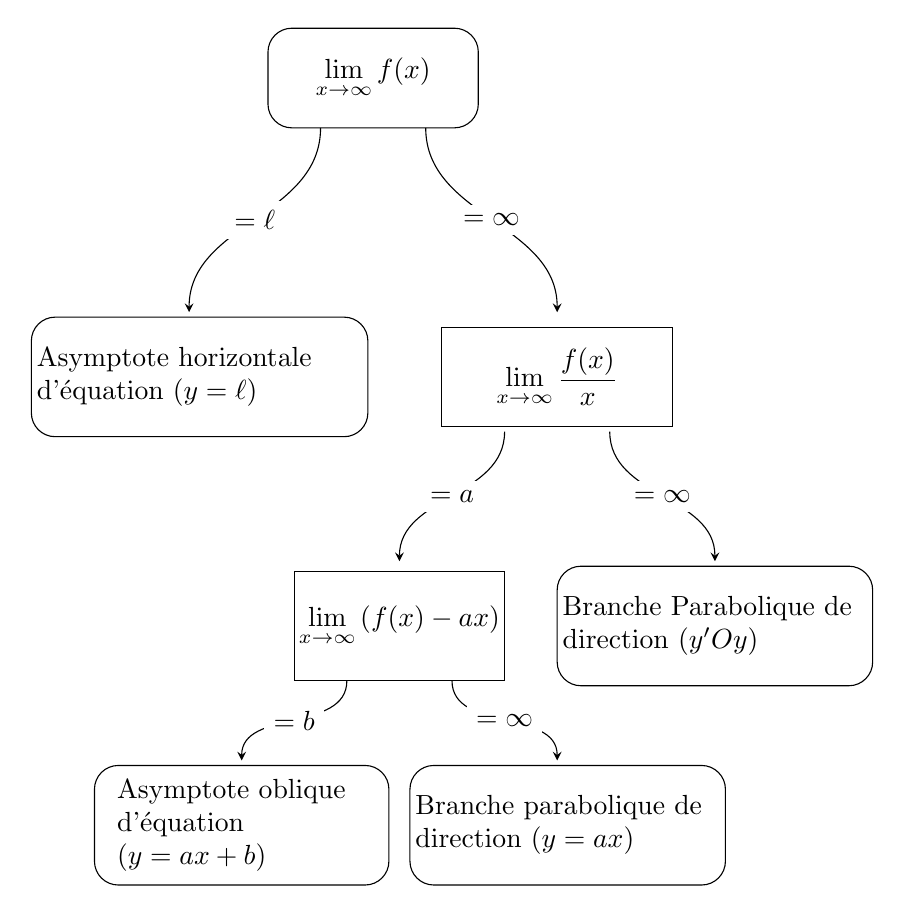
\begin{tikzpicture}[>=stealth,x=1.9em,y=3\baselineskip]
                        \draw[rounded corners = 2ex] (-0.5,6.5) rectangle (3.5,7.5);
                              \draw (1.5,7) node[] {$\displaystyle{ \lim_{x\rightarrow\infty} f(x) }$};
                        \draw[->] (0.5,6.5) to[out=270,in=90] node[fill=white]{$ = \ell$} (-2,4.65);
                        \draw[rounded corners = 2ex] (-5,3.4) rectangle (1.4,4.6);
                              \draw (-2,4) node[] {  \parbox{11em}{\raggedright %
                                                                    Asymptote horizontale d'\'equation  $(y=\ell)$}  };
                        \draw[->] (2.5,6.5) to[out=270,in=90] node[fill=white]{$ = \infty$} (5,4.65);
                        \draw (7.2,3.5) rectangle (2.8,4.5);
                              \draw (5,4) node[] {  $\displaystyle{ \lim_{x\rightarrow\infty} \frac{f(x)}{x} }$  };
                        \draw[->] (6,3.45) to[out=270,in=90] node[fill=white]{$ = \infty$} (8,2.15);
                        \draw[rounded corners = 2ex] (5,2.1) rectangle (11,0.9);
                              \draw (8,1.5) node[] {  \parbox{11em}{\raggedright %
                                                                    Branche Parabolique de direction $(y'Oy)$}  };
                        \draw[->] (4,3.45) to[out=270,in=90] node[fill=white]{$ = a$} (2,2.15);
                        \draw (0,2.05) rectangle (4,0.95);
                              \draw (2,1.5) node[] {  $\displaystyle{\lim_{x\rightarrow\infty} \left( f(x)-ax \right) }$  };
                        \draw[->] (1,0.95) to[out=270,in=90] node[fill=white]{$ = b$} (-1,0.15);
                        \draw[rounded corners = 2ex] (-3.8,0.1) rectangle (1.8,-1.1);
                              \draw (-1,-.5) node[] {  \parbox{9em}{\raggedright %
                                                                     Asymptote oblique d'\'equation $(y=ax+b)$}  };
                        \draw[->] (3,0.95) to[out=270,in=90] node[fill=white]{$ = \infty$} (5,0.15);
                        \draw[rounded corners = 2ex] (2.2,0.1) rectangle (8.2,-1.1);
                              \draw (5.2,-.5) node[] {  \parbox{11em}{\raggedright %
                                                                    Branche parabolique de direction $(y = ax)$}  };
                  \end{tikzpicture}
            \caption{Branches infinies}
\index{Asymptote!horizontale}
\index{Branche parabolique}
            \label{fig:branches infinies}
            \end{figure}

      \smallnota{%
                  Si $\lim_{x\rightarrow\infty} f(x) = \infty$ et que $\lim_{x\rightarrow\infty} \frac{f(x)}{x} = 0$ alors la courbe $\mathscr{C}$ admet une branche parabolique de direction $x'Ox$.
                  }

\TCDLessonStyleOff
\providecommand{\Milimetre}[2]{%
									\clip (#1) rectangle (#2);
									\draw [xstep=0.1cm,ystep=0.1cm,opacity=.05,line width=.05] (#1) grid (#2) ;
									\draw [xstep=0.5cm,ystep=0.5cm,opacity=0.1,line width=0.1] (#1) grid (#2) ;
									\draw [xstep=1.0cm,ystep=1.0cm,opacity=0.2,line width=0.2] (#1) grid (#2) ;
									}
\providecommand{\Courbe}{(\mathscr{C})}
\clearpage
%\begin{fiche}
\index{Courbe!Branches infinies!Branches paraboliques}
	\subsection*{Branches paraboliques}
\index{Branches paraboliques}
		\subsubsection*{Axe $(x'Ox)$}
\index{Branches paraboliques!suivant x'Ox@suivant $(x'Ox)$}
\index{Courbe!Branches paraboliques!suivant x'Ox@suivant $(x'Ox)$}
\vspace{-1.5\baselineskip}
	\[
		\begin{multiform}
			\lim_{x\rightarrow \infty} f(x) = \infty 		\\
			\lim_{x\rightarrow \infty} \frac{f(x)}{x} = 0 .
		\end{multiform}
	\]
La courbe $\Courbe$ admet une branche parabolique de direction $(x'Ox)$ 
		\begin{figure}[h!b]
		\centering
			\begin{tikzpicture}[x=1cm,y=.75cm]
				\shade[right color=loko1, left color=white, opacity=.25] (0,-4) rectangle (5,4);
					\draw[color=loko1] (5,-4) node[below left] {au voisinage de $+\infty$.};
				\shade[left color=loko2, right color=white, opacity=.25] (0,-4) rectangle (-5,4);
					\draw[color=loko2] (-5,-4) node[below right] {au voisinage de $-\infty$.};
				\clip (-5,-4) rectangle (5,4);
				\draw[smooth,samples=10,domain=1:3,color=loko1] plot({(\x)^2},{\x});
					\draw (3,2) node[above] {$\displaystyle{\lim_{x\rightarrow+\infty} f(x) = +\infty}$};
				\draw[smooth,samples=10,domain=1:3,color=loko2] plot({(\x)^2},{-\x});
					\draw (3,-2) node[below] {$\displaystyle{\lim_{x\rightarrow+\infty} f(x) = -\infty}$};
				\draw[smooth,samples=10,domain=1:3,color=loko1] plot(-{(\x)^2},{\x});
					\draw (-3,2) node[above] {$\displaystyle{\lim_{x\rightarrow-\infty} f(x) = +\infty}$};
				\draw[smooth,samples=10,domain=1:3,color=loko2] plot(-{(\x)^2},{-\x});
					\draw (-3,-2) node[below] {$\displaystyle{\lim_{x\rightarrow-\infty} f(x) = -\infty}$};
				\begin{scope}
					\clip (0,0) circle (2);
					\fill[color=white] (0,0) circle (2);
						\shade[right color=loko1, left color=white, opacity=.25] (0,-5) rectangle (5,5);
							\draw[color=loko1] (5,-5) node[below left] {au voisinage de $+\infty$.};
						\shade[left color=loko2, right color=white, opacity=.25] (0,-5) rectangle (-5,5);
							\draw[color=loko2] (-5,-5) node[below right] {au voisinage de $-\infty$.};
				\end{scope}
				\draw[->] (-5,0) -- (5,0);
				\draw[->] (0,-4) -- (0,4);
			\end{tikzpicture}
			\caption{Branches paraboliques suivants l'axe des abscisses.}
		\end{figure}

		\subsubsection*{D'axe $(y'Oy)$}
\index{Branches paraboliques!suivant y'Oy@suivant $(y'Oy)$}
\index{Courbe!Branches paraboliques!suivant y'Oy@suivant $(y'Oy)$}
\vspace{-1.5\baselineskip}
	\[
		\begin{multiform}
			\lim_{x\rightarrow \infty} f(x) = \infty 		\\
			\lim_{x\rightarrow \infty} \frac{f(x)}{x} = \infty 
		\end{multiform}
	\]
La courbe $\Courbe$ admet une branche parabolique de direction $(y'Oy)$ 
		\begin{figure}[h!b]
		\centering
			\begin{tikzpicture}[x=1cm,y=.6cm]
				\shade[right color=loko1, left color=white, opacity=.25] (0,-5) rectangle (5,5);
					\draw[color=loko1] (5,-5) node[below left] {au voisinage de $+\infty$.};
				\shade[left color=loko2, right color=white, opacity=.25] (0,-5) rectangle (-5,5);
					\draw[color=loko2] (-5,-5) node[below right] {au voisinage de $-\infty$.};
				\clip (-5,-5) rectangle (5,5);
				\draw[smooth,samples=10,domain=1:3,color=loko1] plot({\x},{(\x)^2});
					\draw (3,1) node[above] {$\displaystyle{\lim_{x\rightarrow+\infty} f(x) = +\infty}$};
				\draw[smooth,samples=10,domain=1:3,color=loko1] plot({-\x},{(\x)^2});
					\draw (3,-1) node[below] {$\displaystyle{\lim_{x\rightarrow+\infty} f(x) = -\infty}$};
				\draw[smooth,samples=10,domain=1:3,color=loko2] plot({\x},-{(\x)^2});
					\draw (-3,1) node[above] {$\displaystyle{\lim_{x\rightarrow-\infty} f(x) = +\infty}$};
				\draw[smooth,samples=10,domain=1:3,color=loko2] plot({-\x},-{(\x)^2});
					\draw (-3,-1) node[below] {$\displaystyle{\lim_{x\rightarrow-\infty} f(x) = -\infty}$};
				\begin{scope}
					\clip (0,0) circle (2);
					\fill[color=white] (0,0) circle (2.5);
						\shade[right color=loko1, left color=white, opacity=.25] (0,-5) rectangle (5,5);
							\draw[color=loko1] (5,-5) node[below left] {au voisinage de $+\infty$.};
						\shade[left color=loko2, right color=white, opacity=.25] (0,-5) rectangle (-5,5);
							\draw[color=loko2] (-5,-5) node[below right] {au voisinage de $-\infty$.};
				\end{scope}
				\draw[->] (-5,0) -- (5,0);
				\draw[->] (0,-5) -- (0,5);
			\end{tikzpicture}
			\caption{Branches paraboliques suivants l'axe des ordonn\'ees.}
		\end{figure}

		\subsubsection*{D'axe $y = ax$}
\index{Branches paraboliques!suivant y = ax@suivant $(y = ax)$}
\index{Courbe!Branches paraboliques!suivant y = ax@suivant $(y = ax)$}
\vspace{-1.5\baselineskip}
	\[
		\begin{multiform}
			\lim_{x\rightarrow \infty} \frac{f(x)}{x} = a 		\\
			\lim_{x\rightarrow \infty} (f(x) - a \, x) = \infty 
		\end{multiform}
	\]
La courbe $\Courbe$ admet une branche parabolique de direction $(y = a x)$ 
		\begin{figure}[h!b]
		\centering
			\begin{tikzpicture}[x=1cm,y=.6cm]
				\shade[right color=loko1, left color=white, opacity=.25] (0,-5) rectangle (5,5);
					\draw[color=loko1] (5,-5) node[below left] {au voisinage de $+\infty$.};
				\shade[left color=loko2, right color=white, opacity=.25] (0,-5) rectangle (-5,5);
					\draw[color=loko2] (-5,-5) node[below right] {au voisinage de $-\infty$.};
				\clip (-5,-5) rectangle (5,5);
				%%% Raha a > 0 %%%
				\draw[color=col0] (-5,-5) -- (5,5) 
													node[very near end,above,sloped] {\textcolor{col0}{$y = ax$}}
													node[very near end,below,sloped] {$a > 0$}
													node[very near start,above,sloped] {\textcolor{col0}{$y = ax$}}
													node[very near start,below,sloped] {$a > 0$};
				\draw[smooth,samples=10,domain=1.5:5,color=loko1] plot({\x},{\x + ln(\x)});
				\draw[smooth,samples=10,domain=2:5,color=loko1] plot({\x},{\x - ln(\x)});
				\draw[smooth,samples=10,domain=-2:-5,color=loko2] plot({\x},{\x + ln(-\x)});
				\draw[smooth,samples=10,domain=-1.5:-5,color=loko2] plot({\x},{\x - ln(-\x)});
				%%% Raha a < 0 %%%
				\draw[color=col0] (-5,5) -- (5,-5) 
													node[very near end,above,sloped] {\textcolor{col0}{$y = ax$}}
													node[very near end,below,sloped] {$a < 0$}
													node[very near start,above,sloped] {\textcolor{col0}{$y = ax$}}
													node[very near start,below,sloped] {$a < 0$};
				\draw[smooth,samples=10,domain=1.5:5,color=loko2] plot({\x},{-\x - ln(\x)});
				\draw[smooth,samples=10,domain=2:5,color=loko2] plot({\x},{-\x + ln(\x)});
				\draw[smooth,samples=10,domain=-2:-5,color=loko1] plot({\x},{-\x - ln(-\x)});
				\draw[smooth,samples=10,domain=-1.5:-5,color=loko1] plot({\x},{-\x + ln(-\x)});
				\begin{scope}
					\clip (0,0) circle (2.5);
					\fill[color=white] (0,0) circle (2.5);
						\shade[right color=loko1, left color=white, opacity=.25] (0,-5) rectangle (5,5);
							\draw[color=loko1] (5,-5) node[below left] {au voisinage de $+\infty$.};
						\shade[left color=loko2, right color=white, opacity=.25] (0,-5) rectangle (-5,5);
							\draw[color=loko2] (-5,-5) node[below right] {au voisinage de $-\infty$.};
				\end{scope}
				\draw[->] (-5,0) -- (5,0);
				\draw[->] (0,-5) -- (0,5);
			\end{tikzpicture}
			\caption{Branches paraboliques suivants la droit d'\'equation ${y = ax}$.}
		\end{figure}
%\end{fiche}


























\TCDLessonStyleOff
\clearpage
\section{Exercices}
      \begin{exo}
      Calculer les limites suivantes : \\
%      \begin{minipage}{0.45\textwidth}
            \begin{itemize}
                  \item $\lim_{x\rightarrow 2}\frac{x^2 - 4}{x-2}$
                  \item $\lim_{x\rightarrow 2^+} \sqrt{x-2}$
                  \item $\lim_{x\rightarrow -2} \sqrt{|x+2| + 2} $
                  \item $\lim_{x\rightarrow-2^+} \frac{x^3 + 8}{|x+2|} $
%            \end{itemize}      
%      \end{minipage}
      %
%      \begin{minipage}{0.45\textwidth}
%            \begin{itemize}
                  \item $ \lim_{x\rightarrow 1} -\frac{1}{(x-1)^2} $
                  \item $ \lim_{x\rightarrow 1^+} \frac{1}{x-1} $
                  \item $ \lim_{x\rightarrow 1^-} \frac{x}{x-1} $
                  \item $ \lim_{x\rightarrow 1^+} \sqrt{\frac{x}{x-1}} $
            \end{itemize}
%      \end{minipage}
      \end{exo}
%
      \begin{exo}~\\
            \begin{enumerate}
                  \item Soit $g(x) = x^3 + x^2 - 8 x - 12$.
                        Calculer $g(-2)$. Factoriser $g(x)$.
                  \item On consid\`ere la fonction $f : x \mapsto \frac{-3x^2-x+10}{x^3+x^2-8x-12}$.
                        Quel est l'ensemble de d\'efinition de $f$?
                        D\'eterminer les limites de $f$ aux bornes de son domaine de d\'efinition.
            \end{enumerate}
      \end{exo}
%
      \begin{exo}~\\
            \begin{enumerate}
                  \item Factoriser les deux polyn\^omes $\varphi$ et $\theta$ tels que :
                        $\varphi (x) = -9x^3 -15x^2 + 8x + 16$ et $\theta (x) = 5x^2 + 7x - 12$.
                  \item On consid\`ere la fonction $f : x \mapsto \frac{\varphi (x)}{\theta (x)}$.
                        Quel est l'ensemble de d\'efinition de $f$\,? 
                        Quelles sont les limites de $f$ aux bornes de son domaine de d\'efinition?
                  \item On consid\`ere la fonction $g : x \mapsto \frac{\theta (x)}{\varphi (x)}$.
                        Quel est l'ensemble de d\'efinition de $g$\,? 
                        Quelles sont les limites de $g$ aux bornes de son domaine de d\'efinition?
            \end{enumerate}
      \end{exo}
%
      \begin{exo}
      Calculer les limites suivantes : \\[\baselineskip]
%            \begin{minipage}{0.45\textwidth}
                  \begin{itemize}
                        \item $ \lim_{x\rightarrow -\infty} \frac{x}{x-1} $
                        \item $ \lim_{x\rightarrow +\infty} \frac{\sqrt{x^3 - 1}}{x \sqrt{x}} $
                        \item $ \lim_{x\rightarrow +\infty} \sqrt{x^2 + 1} - x $
                        \item $ \lim_{x\rightarrow -\infty} \sqrt{|x^3 - 1|} + x^2 $
                        \item $ \lim_{x\rightarrow 3} \frac{\sqrt{x+1}-2}{x-3} $
                        \item $ \lim_{x\rightarrow 2} \frac{\sqrt{x+2}-2}{\sqrt{x+7}-3} $
                        \item $ \lim_{x\rightarrow 0} \frac{x}{\sqrt{x^2+1} - 1} $
%                  \end{itemize}            
%            \end{minipage}
%            %
%            \begin{minipage}{0.45\textwidth}
%                  \begin{itemize}
                        \item $ \lim_{x\rightarrow +\infty} \sqrt{x^2+2x+5}-\sqrt{x^2-1} $
                        \item $ \lim_{x\rightarrow -\infty} \sqrt{x^2+2x+5}-\sqrt{x^2-1} $
                        \item $ \lim_{x\rightarrow +\infty} \sqrt{x^2+x+1}-3x+2 $
                        \item $ \lim_{x\rightarrow -\infty} \sqrt{x^2+x+1}-3x+2 $
                        \item $ \lim_{x\rightarrow +\infty} \sqrt{x^2+x+1}+x+2 $
                        \item $ \lim_{x\rightarrow -\infty} \sqrt{x^2+x+1}+x+2 $
                        \item $ \lim_{x\rightarrow +\infty} \sqrt{x+\sqrt{x}} - \sqrt{x} $            
                  \end{itemize}
%            \end{minipage}
      \end{exo}
%
      \begin{exo}
            On consid\`ere la fonction $f$ telle que $f(x) = \sqrt{\frac{x^3}{x-1}}$.
            \begin{enumerate}
                  \item Quel est l'ensemble de d\'efinition de $f$.
                        Quelle est la limite de $f(x)$ lorsque $x$ tend vers $\pm \infty$.
                  \item D\'eterminer $\lim_{x\rightarrow+\infty} \frac{f(x)}{x}$. On note par $a$ cette limite.
                        Calculer $\lim_{x\rightarrow+\infty} f(x) - ax$, on note par $b$ cette limite.
                  \item On pose $\varepsilon (x) = f(x) - (ax + b)$.
                        Etudier le signe de $\varepsilon (x)$.
                        Que peut-on en d\'eduire\,?
            \end{enumerate}
      \end{exo}
%
      \begin{exo}
            On consid\`ere la fonction $f:x\mapsto\frac{1-x}{1+x}$.
            D\'eterminer les constantes $a$ et $b$ telles que $f(x) = a + \frac{b}{1+x}$.
             la  la d\'eriv\'ee $n^\text{i\`eme}$ de $f$.
      \end{exo}
%
      \begin{exo}
            Soit $f$ la fonction d\'efinie sur $]-1 ; +\infty[$ par $f(x) = x + 3 + \frac{2}{x+1}$.
            \begin{enumerate}
                  \item D\'eterminer $\lim_{x\rightarrow-1} f(x)$.
                        Que peut-on en d\'eduire comme asymptote pour la courbe repr\'esentative $(\mathscr{C})$ de $f$\,?
                  \item D\'eterminer $\lim_{x\rightarrow+\infty} f(x)$.
                  \item D\'eterminer $\lim_{x\rightarrow+\infty} \left[ f(x) - (x+3) \right]$.
                        Que peut-on en d\'eduire comme asymptote pour la courbe repr\'esentative $(\mathscr{C})$ de $f$\,?
            \end{enumerate}
      \end{exo}
%
      \begin{exo}
            On consid\`ere la fonction $f$ d\'efinie par $f(x) = \frac{1+x^2}{1-x^2}$.
            \begin{enumerate}
                  \item Donner le domaine de d\'efinition de $f$.
                  \item Calculer les limites de $f$ aux bornes de son domaine de d\'efinition.
                  \item D\'eterminer la fonction $f'$, fonction d\'eriv\'ee de $f$.
                  \item \'Etudier le signe de $f'$ puis dresser le tableau des variations de $f$.
                  \item Tracer la courbe $(\mathscr{C})$ repr\'esentative de $f$ dans un rep\`ere orthonorm\'e.
            \end{enumerate}
            M\^eme questions pour les fonctions : $g:x\mapsto x+\sqrt{16-x^2} $ et $h:x\mapsto\sqrt{|x^2-6x-7|}$.
      \end{exo}
%
      \begin{exo}
            Etudier la fonction $f : x \mapsto \frac{x^3 + 2}{2x}$ et 
            construire sa courbe repr\'esentative $(\mathscr{C})$ dans un rep\`ere orthonorm\'e.
            Placer dans le m\^eme rep\`ere la parabole $(\mathscr{P})$ d'\'equation $p(x) = \frac{x^2}{2}$.
      \end{exo}
%
      \begin{exo}
            Soit la fonction $f : x \mapsto \sqrt{x^2 + x + 1}$ et notons par $(\mathscr{C})$ sa courbe repr\'esentative.
            Montrer que $(\mathscr{C})$ admet un axe de sym\'etrie, puis construire $(\mathscr{C})$ dans un rep\`ere orthonorm\'e.
      \end{exo}
%
      \begin{exo}
            On consid\`ere la fonction $f:x\mapsto \frac{x}{1+|x|}$ et on note par $(\mathscr{C})$ sa courbe repr\'esentative.

            Etudier le sens de variation de $f$, 
            en d\'eduire que $f$ admet une fonction r\'eciproque $f^{-1}$ dont on d\'eterminera le domaine de d\'efinition.
            On note par $(\mathscr{C}')$ la courbe repr\'esentative de $f^{-1}$.
            
            Exprimer $f^{-1} (x)$ en fonction de $x$.
            Construire $(\mathscr{C})$ et $(\mathscr{C}')$ dans le m\^eme rep\`ere.
      \end{exo}
%
      \begin{exo}
            On consid\`ere la fonction $f$ d\'efinie par :
                  \[
                        \left\lbrace
                              \begin{array}{l}
                                    f(x) = \frac{|x| \sqrt{|x|}}{x} \quad \forall x \in \mathbb{R}^*\\
                                    f(0) = 0
                              \end{array}
                        \right.
                  \]
            \begin{enumerate}
                  \item Etudier la continuit\'e et la d\'erivabilit\'e de $f$ en $0$.
                  \item D\'emontrer que $f$ admet une fonction r\'eciproque $f^{-1}$ 
                        dont on pr\'ecisera l'ensemble de d\'efinition.
                        Exprimer $f^{-1} (x)$ en fonction de $x$.
                  \item Repr\'esenter graphiquement $f$ et $f^{-1}$ dans un rep\`ere orthonorm\'e.
            \end{enumerate}
      \end{exo}
%
      \begin{exo}
      On consid\`ere la fonction $f:x\mapsto 1+\frac{x}{\sqrt{x^2 + 1}}$.
      On note par $(\mathscr{C})$ sa courbe repr\'esentative dans un rep\`ere orthonorm\'e $(O,\vec{\imath},\vec{\jmath})$.
      \begin{enumerate}
            \item 
%                  \begin{enumerate}
%                        \item 
                              Etudier les variations de $f$.
%                        \item 
                              Montrer que $(\mathscr{C})$ admet un point d'inflexion $I$ que l'on d\'eterminera.
%                        \item 
                              D\'eterminer l'\'equation de la tangente en $I$ \`a la courbe $(\mathscr{C})$.
%                        \item 
                              Montrer que $(\mathscr{C})$ admet $I$ comme centre de sym\'etrie.
%                        \item 
                              Construire $(\mathscr{C})$.
%                  \end{enumerate}
            \item Montrer que l'\'equation $f(x) = x$ admet une solution $\alpha \in ]1,2[$.
                  On pourra appliquer le th\'eor\`eme des valeurs interm\'ediaires \`a la fonction $g : x \mapsto f(x) - x$.
            \item 
                  %\begin{enumerate}
%                        \item 
                              Montrer que $f$ est une bijection de $\mathbb{R}$ sur un intervalle de $\mathbb{R}$.
%                        \item 
                              D\'eterminer l'ensemble de d\'efinition et l'ensemble d'arriv\'e de 
                              sa fonction r\'eciproque $f^{-1}$.
%                        \item 
                              Exprimer $f^{-1}(x)$ en fonction de $x$.
%                        \item 
                              Construire la courbe $(\mathscr{C}')$, repr\'esentative de $f^{-1}$ 
                              dans $(O,\vec{\imath},\vec{\jmath})$.            
%                  \end{enumerate}
      \end{enumerate}
      \end{exo}
%%%%%%%%%% Fonction irrationnelle
\begin{exo}
Soit $f$ la fonction d\'efinie par : 
$\displaystyle{
f(x) = x + \sqrt{|4x^2 - 1|}
}$
et notons par $(\mathcal{C})$ sa courbe repr\'esentative.
\begin{enumerate}
\item Donner le domaine de d\'efinition de $f$.
\item Etudier la continuit\'e de $f$.
\item Etudier la d\'erivabilit\'e de $f$ aux points $-\frac{1}{2}$ et $\frac{1}{2}$.
\item Donner la fonction d\'eriv\'ee de $f$.
\item Etudier les signes de : 
     \begin{enumerate}
     \item $\sqrt{4x^2 - 1} + 4x$.
     \item $\sqrt{1 - 4x^2} - 4x$.
     \end{enumerate}
\item Etudier les signes de $f'$; en d\'eduire le tableau de variation de $f$.
\item Calculer $\lim_{x \rightarrow - \infty} \left( f(x) + x \right)$ et $\lim_{x \rightarrow + \infty} \left( f(x) - 3 x \right) $.
      Interpreter le r\'esultat en terme de branches infinies.
\item Tracer la courbe repr\'esentative de $f$ dans un rep\`ere orthogonal $(O, \vec{\imath},\vec{\jmath})$ o\`u $\|\vec{\imath}\| = \text{4cm}$ et $\| \vec{\jmath} \| = \text{ 2 cm } $.
\item 
      \begin{enumerate}
      \item Soit $h$ la restriction de $f$ \`a l'intervalle $]-\infty ; -\frac{1}{2} ]$.
            Montrer que $h$ admet une fonction r\'eciproque $h^{-1}$ dont on pr\'ecisera l'ensemble de d\'epart et la variation.
      \item Calculer $\lim_{x \rightarrow + \infty} \left[ x + h^{-1} (x) \right]$, conclure et tracer la courbe $(\Gamma)$ repr\'esentative de $h^{-1}$.
      \item Calculer $h^{-1} (0)$ et d\'eterminer une \'equation de la tangente \`a $(\Gamma)$ au point $O$.
      \end{enumerate}
\end{enumerate}
\end{exo}


% T12 C/D, chapitre 10 : Fonctions exponentielle et logarithme. Source : le livre « Terminales scientifiques » (ExpoLog/Lesona, ExpoLog/Exo).
% Les exercices tirés d’autres ouvrages ne sont pas repris (décision du 2 novembre 2026).

\TCDLessonStyleOn
\chapter{Fonction exponentielle et logarithme}
\section{Fonction exponentielle}
      \begin{defi}
      \index{Fonction!exponentielle}
            La \emph{fonction exponentielle} est l'unique fonction $f$ d\'efinie sur $\mathbb{R}$ et v\'erifiant : 
                  \[   f' = f \qquad \text{ et } \qquad f(0) = 1   \,. \]
            On note la fonction par $\mathrm{exp}$.
      \end{defi}
      %
      \begin{prop}
            La fonction exponentielle peut en fait \^etre consid\'er\'e comme une fonction puissance.
            Il existe un nombre r\'eel $e$ ($\simeq 2,718\,281\,828\,459\,045$) 
            tel que $\exp{x} = e^{x}$ pour tout $x\in\mathbb{Q}$.
            
            Ainsi, dor\'enavant, on consid\`erera la fonction exponentielle comme 
            une g\'en\'eralisation d'une fonction puissance.
            On d\'enotera alors $\exp{x}$ par $\expo{x}$.
      \end{prop}
      %
      \begin{thm}
            Soient $a$ et $b$ deux nombres r\'eels.
            \begin{itemize}
                  \item $\expo{0} = 1$
                  \item $\expo{a+b} = \expo{a} \cdot \expo{b}$
                  \item $\expo{-a} = \frac{1}{\expo{a}}$
                  \item $\expo{a-b} = \frac{\expo{a}}{\expo{b}}$
                  \item $\forall n \in \mathbb{Q},\ \left(\expo{a}\right)^n = \expo{na}$.
            \end{itemize}
      \end{thm}
      %
      \begin{prop}
            La fonction $\exp$ est d\'efinie sur $\mathbb{R}$.
            De plus, $\expo{x} > 0$ pour tout $x\in\mathbb{R}$.
            Comme $\exp' x = \exp x > 0$, alors la fonction $\exp$ est strictement croissante sur $\mathbb{R}$.
            Il suit que, pour tout $(x,y)\in\mathbb{R}^2$ :
                  \[
                        x<y \Rightarrow \expo{x} < \expo{y}      \;.
                  \]
      \end{prop}
      %
      \begin{thm}[Limites usuelles sur la fonction $\exp$]
            \begin{align*}
                  \lim_{x\rightarrow-\infty} \expo{x} & = 0     & \lim_{x\rightarrow+\infty} \expo{x} & = +\infty \\
                  \lim_{x\rightarrow-\infty} x \expo{x} & = 0   & \lim_{x\rightarrow+\infty} \frac{\expo{x}}{x} & = +\infty \\
                \intertext{ou plus g\'en\'eralement, pour tout $n\in\mathbb{N}$}
                  \lim_{x\rightarrow-\infty} x^n \expo{x} & = 0 & \lim_{x\rightarrow+\infty} \frac{\expo{x}}{x^n} & = +\infty\;.
            \end{align*}
            On a aussi 
                  \[
                        \lim_{x\rightarrow 0} \frac{\expo{x}-1}{x} = 1      \;.
                  \]
      \end{thm}
      %
      \paragraph{Fonctions compos\'ees avec la fonction exponentielle}
            Il suit de la formule de d\'erivation d'une fonction compos\'ee que 
            $\left( \expo{u} \right)' = u' \expo{u}$.
            Ainsi, $u$ et $\expo{u}$ ont m\^eme sens de variations.
      \paragraph{\'Etude de la fonction $\exp$}~\\
      Posons $f(x) = \expo{x}$.
            \begin{description}
            \item[Domaine de d\'efinition :] La fonction $\exp$ est d\'efinie sur $\mathbb{R} = ]-\infty,+\infty[$.
            \item[Limites aux bornes :] $\lim_{x\rightarrow -\infty} \expo{x} = 0$ et 
                                        $\lim_{x\rightarrow +\infty} \expo{x} = +\infty$
            \item[D\'eriv\'ee :] Pour tout $x\in\mathbb{R}$, $f'(x) = \expo{x}$.
            \item[Tableau des variations :]~\\[-1\baselineskip]
                  \begin{table}[H]
                  \centering
                        \begin{tikzpicture}[>=stealth,scale=.75]
                        \draw (-2,0) -- (4,0);
                        \draw (-2,-1) -- (4,-1);
                        \draw (0,.5) -- (0,-2);
                        \draw (-1,.25) node[] {$x$};
                        \draw (-1,-.5) node[] {$f'(x)$};
                        \draw (-1,-1.5) node[] {$f(x)$};
                        \draw (.5,.25) node[] {$-\infty$};
                        \draw (3.5,.25) node[] {$+\infty$};
                        \draw (2,-.5) node[] {$+$};
                        \draw (.5,-1.75) node[] {$0$};
                        \draw (3.5,-1.25) node[] {$+\infty$};
                        \draw[->] (.75,-1.75) -- (3,-1.25);
                        \end{tikzpicture}
                  \caption{Tableau des variations de la fonction exponentielle.}
                  \label{tab:variations expo}
                  \end{table}
            \item[Valeurs remarquables :] $f(0) = 1$ donc la courbe passe par le point de coordonn\'es $(0,1)$.
                                          De plus, la d\'eriv\'ee en ce point est \'egale \`a $1$,
                                          ce qui signifie que la pente de la tangente en ce point 
                                          est parall\`ele \`a la premi\`ere bissectrice.
                                          $f(1) = \expo{}$ donc la courbe passe par le point de coordonn\'es $(1,\expo{})$. 
            \item[Courbe repr\'esentative :]
                  Avant de tracer la courbe repr\'esentative de $f$, \'etudions d'abord ses branches infinies.
                  \begin{itemize}
                        \item Comme $\lim_{x\rightarrow-\infty} f(x) = 0$, 
                              alors la courbe admet la droite d'\'equation $y=0$ comme asymptote horizontale
                              au voisinage de $-\infty$.
                        \item Comme $\lim_{x\rightarrow+\infty} f(x) = +\infty$ et que
                              $\lim_{x\rightarrow+\infty} \frac{f(x)}{x} = +\infty$ alors
                              la courbe admet une branche parabolique suivant $y'Oy$.
                  \end{itemize}
            \begin{figure}[h!]
            \centering
                  \begin{tikzpicture}[line cap=round,line join=round,>=stealth,scale=.9]
                  \draw[->,color=black] (-4.2,0) -- (5.24,0);
                  \foreach \x in {-4,-3,-2,-1,1,2,3,4,5}
                  \draw[shift={(\x,0)},color=black] (0pt,2pt) -- (0pt,-2pt) node[below] {\footnotesize $\x$};
                  \draw[->,color=black] (0,-4.2) -- (0,5.3);
                  \foreach \y in {-4,-3,-2,-1,1,2,3,4,5}
                  \draw[shift={(0,\y)},color=black] (2pt,0pt) -- (-2pt,0pt) node[left] {\footnotesize $\y$};
                  \draw[color=black] (0pt,-10pt) node[right] {\footnotesize $0$};
                  \clip(-4,-4) rectangle (5.7,5.7);
                  \draw[dashed] (0,2.718281828) -- (1,2.718281828);
                  \draw[dashed] (1,0) -- (1,2.718281828);
                  \draw[color=loko1, smooth,samples=100,domain=0:1.6, thick] 
                                                                  plot(\x,{2.718281828^(\x)}) node[fill=white] {$y=\expo x$};
                  \draw[color=loko1, smooth,samples=100,domain=0:5, thick] plot({-\x},{1/(2.718281828^(\x))});
                  \draw[color=loko3, smooth,samples=100,domain=-4:4, thick] plot(\x,{(\x)+1}) node[fill=white] {$y=x+1$};
                  \filldraw[fill=loko1, draw=loko2] (0,1) circle (.2em);
                  \filldraw[fill=loko1, draw=loko2] (1,2.718281828) circle (.2em);
                  \end{tikzpicture}
            \caption{Courbe repr\'esentative de la fonction $\exp$.}
            \label{fig:courbe exp}
            \end{figure}
            \end{description}
            

\section{Fonction Logarithme}
      \subsection{Logarithme n\'ep\'erien}
      \begin{defi}
      \index{Fonction!Logarithme neperien@Logarithme n\'ep\'erien}
            On a vu que la fonction exponentielle est continue (elle est m\^eme d\'erivable)
            et strictement croissante sur $\mathbb{R}$.
            Elle d\'efinit donc une bijection de $\mathbb{R}$ vers $\mathbb{R}^*_+$.
            On définit la fonction logarithme népérien comme étant la fonction r\'eciproque de la fonction exponentielle.
            Ainsi, 
            $\ln : \mathbb{R}^*_+   \rightarrow   \mathbb{R}$ v\'erifie :
                  \[
                        \left\lbrace
                              \begin{array}{ll}
                                    \forall x\in\mathbb{R}      ,&  \ln(\expo{x}) = x \\
                                    \forall x\in\mathbb{R}^*_+  ,&  \expo{\ln x} = x  \;.
                              \end{array}
                        \right.
                  \]
      \end{defi}
      Ainsi, la courbe de la fonction $\exp$ et celle de la fonction $\ln$ sont 
      sym\'etriques par rapport \`a la premi\`ere bissectrice.
            \begin{figure}[h!]
            \centering
                  \begin{tikzpicture}[line cap=round,line join=round,>=stealth,scale=.9]
                  \draw[->,color=black] (-4.2,0) -- (5.24,0);
                  \foreach \x in {-4,-3,-2,-1,1,2,3,4,5}
                  \draw[shift={(\x,0)},color=black] (0pt,2pt) -- (0pt,-2pt) node[below] {\footnotesize $\x$};
                  \draw[->,color=black] (0,-4.2) -- (0,5.3);
                  \foreach \y in {-4,-3,-2,-1,1,2,3,4,5}
                  \draw[shift={(0,\y)},color=black] (2pt,0pt) -- (-2pt,0pt) node[left] {\footnotesize $\y$};
                  \draw[color=black] (0pt,-10pt) node[right] {\footnotesize $0$};
                  \clip(-4,-4) rectangle (5.7,5.7);
                  \draw[color=loko2, smooth,samples=100,domain=0.001:5, thick] 
                        plot(\x,{ln((\x))}) node[fill=white,sloped,above left] {$y=\ln x$};
                  \draw[color=loko1, smooth,samples=100,domain=0:1.6, thick] 
                                                                  plot(\x,{2.718281828^(\x)}) node[fill=white] {$y=\expo x$};
                  \draw[color=loko1, smooth,samples=100,domain=0:5, thick] plot({-\x},{1/(2.718281828^(\x))});
                  \draw[color=loko3, smooth,samples=100,domain=-4:5, thick] plot(\x,{(\x)}) node[fill=white] {$y=x$};
                  \end{tikzpicture}
            \caption{Courbe des fonctions $\exp$ et $\ln$.}
            \label{fig:exp et ln}
            \end{figure}
      %
      \begin{rmk}[Valeurs remarquables]~\\[-1\baselineskip]
            \begin{itemize}
                  \item $\ln 1 = 0$ car $\expo{0} = 1$
                  \item $\ln \expo{} = 1$ car $\expo{1} = \expo{}$.
            \end{itemize}
            Comme la fonction exponentielle est continue et strictement croissante de $\mathbb{R}$ sur $]0,+\infty[$, 
            la fonction Logarithme n\'ep\'erienne est continue et strictement croissante $]0,+\infty[$ sur $\mathbb{R}$.
      \end{rmk}
      %
      \begin{prop}[Propri\'et\'es alg\'ebriques]
            Soient $a$ et $b$ deux nombres r\'eels positifs et $n$ un entier relatif.
            On a alors :\\
            \begin{align*}
                        \ln (a\cdot b) & = \ln a + \ln b                                                &       
                        \ln (a^n) & = n \cdot \ln a                                                     \\
                        \ln \frac{1}{a} & = - \ln a                                                     & 
                        \ln \frac{a}{b} & = \ln a - \ln b                                               \\
                        \ln a < \ln b & \iff a < b                                                      & 
                        \ln a = \ln b & \iff a = b                                                      \\
                        \forall \lambda \in \mathbb{R},\ \ln x = \lambda & \iff x = \expo{\lambda}      & 
                        \forall \lambda \in \mathbb{R}^*_+,\ \expo{x} = \lambda & \iff x = \ln{\lambda} \\
                        \forall \lambda \in \mathbb{R},\ \ln x < \lambda & \iff x < \expo{\lambda}      & 
                        \forall \lambda \in \mathbb{R}^*_+,\ \expo{x} < \lambda & \iff x < \ln{\lambda} \\
            \end{align*}
      \end{prop}
      %
      \begin{thm}[D\'eriv\'ee de la fonction $\ln$]
            La fonction logarithme n\'ep\'erien est d\'erivable sur $]0,+\infty[$ avec
                  \begin{equation*}
                        \left( \ln x \right)' = \frac{1}{x}      \;.
                  \end{equation*}
            \begin{proof}
                  Posons $f(x) = \expo{x}$. On sait alors que $f^{-1} (x) = \ln x$.
                  En utilisant la formule de d\'erivation de la fonction r\'eciproque, on a :
                        \begin{align*}
                              \left(f^{-1}\right)' (x)  & = \frac{1}{f' \left( f^{-1} (x) \right) }      \\
                              \left(\ln (x) \right)'    & = \frac{1}{\expo{\ln x}}                       \\
                              \left(\ln (x) \right)'    & = \frac{1}{x}                                  \,.
                        \end{align*}
            \end{proof}
      \end{thm}
      %
      \begin{thm}[Limites usuelles]~\\
                  \begin{align*}
                        \lim_{x\rightarrow 0^+} \ln x                & = -\infty            &
                        \lim_{x\rightarrow 0^+} x\cdot\ln x          & = 0                  \\
                        \lim_{x\rightarrow +\infty} \ln x            & = +\infty            &
                        \lim_{x\rightarrow +\infty} \frac{\ln x}{x}  & = 0                  
                  \end{align*}
                  \[
                        \lim_{x\rightarrow 0} \frac{\ln (1 + x)}{x} = 1      \;.
                  \]
      \end{thm}
      %
      \paragraph{Fonctions compos\'ees avec la fonction logarithme n\'ep\'erien}
            Soit $u$ une fonction d\'erivable sur un intervalle $I$ tel que $u(x)>0$ pour tout $x\in I$.
            Il suit de la formule de d\'erivation d'une fonction compos\'ee que 
            $\left( \ln {u} \right)' = \frac{u'}{u}$.
            Ainsi, $u$ et $\ln{u}$ ont m\^eme sens de variations.
      %
            
      %
      \subsection{Logarithme de base quelconque}
            \begin{defi}[Logarithme d\'ecimal]
                  On d\'efinit la fonction logarithme d\'ecimal par :
                        \begin{equation*}
                              \begin{array}{rcl}
                                    \log :\ ]0,+\infty[ & \rightarrow & \mathbb{R}      \\
                                                     x & \mapsto     & \frac{\ln x}{\ln 10}
                              \end{array}
                        \end{equation*}
            \end{defi}
            %
            \begin{prop}
                  Si la fonction $\ln$ est la r\'eciproque de la fonction $x\mapsto \expo{x}$,
                  la fonction $\log$ peut \^etre consid\'er\'ee comme \'etant la r\'eciproque de la fonction $x\mapsto 10^x$.
                  
                  Ainsi, si $n$ est un nombre entier naturel, l'\'ecriture d\'ecimale de $n$ comporte 
                  $\entiere{\log (n)}+1$ chiffres.
                        \begin{ex}
                              Le plus grand nombre premier connu \`a ce jour (mai 2018)%
                                    \footnote{%
                                    D\'ecouvert en d\'ecembre 2017 par le GIMPS en d\'ecembre 2017.
                                                }
                              est $2^{77\, 232\, 917} - 1$.
                              Puisqu'il s'agit d'un nombre premier, 
                              il comporte le m\^eme nombre de chiffre que le nombre $2^{77\, 232\, 917}$.
                              Pour calculer le nombre de chiffres qu'il comporte, on effectue :
                                    \[
                                           \log (2^{77\, 232\, 917})
                                    =      \frac{\ln (2^{77\, 232\, 917})}{\ln 10} 
                                    =      \frac{77\, 232\, 917 \cdot \ln 2}{\ln 10}
                                    \simeq 23\,249\,424,66962662
                                    .
                                    \]
                              Ainsi, ce nombre comporte $23\,249\,425$ chiffres.
                        \end{ex}
            \end{prop}
            \begin{defi}[Logarithme de base $a$]
                  Soit $a$ un nombre r\'eel strictement positif.
                  On d\'efinit la fonction logarithme de base $a$ par :
                        \begin{equation*}
                              \begin{array}{rcl}
                                    \log_a :\ ]0,+\infty[ & \rightarrow & \mathbb{R}                        \\
                                                        x & \mapsto     & \frac{\ln x}{\ln a}               \;.
                              \end{array}
                        \end{equation*}
            \end{defi}
      %
      




\TCDLessonStyleOff
\clearpage
\providecommand{\ivec}{\vec{\imath}}
\providecommand{\jvec}{\vec{\jmath}}
\providecommand{\Oij}{$(O,\ivec,\jvec)$ }
%%%%%%%%%%%%%%%%%%%%%%%%%%%%%%%%%%%%%%%%%%%%%%%%%%%%%%%%%%%%%%%%%%%%%%%%%%%%%%%%%%%
%%%%%%%%%%%%%%%%%%%%%%%%%%%%%%%%%%%%%%%%%%%%%%%%%%%%%%%%%%%%%%%%%%%%%%%%%%%%%%%%%%%
\section{Exercices}
%%%%%%%%%%%%%%%%%%%%%%%%%%%%%%%%%%%%%%%%%%%%%%%%%%%%%%%%%%%%%%%%%%%%%%%%%%%%%%%%%%%
\begin{exo}
\begin{description}
\item[A.] On consid\`ere la fonction $\varphi$ d\'efinie sur $\mathbb{R}$ par $\varphi(x) = \expo{x} + x + 1$.
      \begin{enumerate}
      \item Dresser le tableau des variations complet de $\varphi$.
      \item Montrer que l'\'equation $\varphi (x) = 0$ admet une unique solution $\alpha$ et que 
            ${\alpha \in \ ] -1,28 \ ; \ -1,27 [}$.
      \item En d\'eduire le signe de $\varphi (x)$ sur $\mathbb{R}$.
      \end{enumerate}
\item[B.] Soit $f$ la fonction d\'efinie sur $\mathbb{R}$ par $f(x) = \frac{x \expo{x}}{\expo{x} + 1}$ et notons par 
      $(\mathcal{C})$ sa courbe repr\'esentative dans un rep\`ere orthonorm\'e $(O , \ivec , \jvec )$ d'unit\'e $4 \text{cm}$.
      \begin{enumerate}
      \item Etudier les variations de $f$.
      \item Montrer que $f(\alpha) = \alpha + 1$.
      \item Calculer les limites de $f$ aux bornes de $\mathbb{R}$ et montrer que la droite $(\mathcal{D})$ d'\'equation 
            $y = x$ est asymptote \`a $(\mathcal{C})$ et \'etudier la position de $(\mathcal{C})$ par rapport \`a $(\mathcal{D})$.
      \item Tracer $(\mathcal{C})$ et $(\mathcal{D})$ dans le m\^eme rep\`ere.
      \end{enumerate}
\end{description}
\end{exo}
%%%%%%%%%%%%%%%%%%%%%%%%%%%%%%%%%%%%%%%%%%%%%%%%%%%%%%%%%%%%%%%%%%%%%%%%%%%%%%%%%%%
\begin{exo} ~ \newline
Soit la fonction num\'erique $f$ d\'efinie sur l'intervalle $]-1 \; ; \; +\infty[$ par :
\begin{displaymath}
f(x) = 
\left\lbrace
\begin{tabular}{lll}
$ - x + 2 \ln (x + 1) $ & si & $ x \in \; ] -1 \; ; \; 0[ $ \\
$ x - 1 + \expo{-x} $ & si & $ x \in [0 \; ; \; + \infty[ $.
\end{tabular}
\right.
\end{displaymath}
On note par $(\mathscr{C})$ sa courbe repr\'esentative dans un rep\`ere orthonorm\'e \Oij d'unit\'e 2 cm.
\begin{enumerate}
\item Montrer que $f$ est continue en $0$.
\item Montrer que $\lim_{x \rightarrow 0^-} \frac{f(x) - f(0)}{x - 0} = 1$ et 
      $\lim_{x \rightarrow 0^+} \frac{f(x) - f(0)}{x - 0} = 0$.
      Que peut-on en conclure sur $f$\,?
\item \begin{enumerate}
      \item Calculer $\lim_{x \rightarrow -1^+} f(x)$ et $\lim_{x \rightarrow +\infty} f(x)$.
      \item Etudier le signe de $f'(x)$ sur les intervalles $]-1 \; ; \; 0[$ et $] 0 \; ; \; +\infty[$.
      \item Dresser le tableau des variations de $f$.
      \end{enumerate}
\item Montrer que la droite $(\mathcal{D})$ d'\'equation $y = x- 1$ est asymptote \`a $(\mathscr{C})$ au voisinage de $+\infty$.
\item Tracer $(\mathscr{C})$ et $(\mathcal{D})$ dans le m\^eme rep\`ere \Oij en pr\'ecisant les demi-tangentes \`a l'origine.
\item Soit $g$ la restriction de $f$ \`a l'intervalle $I = [ 0 \; ; \; +\infty[$.
      \begin{enumerate}
      \item Montrer que $g$ admet une r\'eciproque $g^{-1}$ dont on d\'eterminera l'ensemble de d\'efinition.
      \item Repr\'esenter $g^{-1}$ dans le m\^eme rep\`ere que $(\mathscr{C})$.
      \end{enumerate}
\end{enumerate}

\end{exo}
%%%%%%%%%%%%%%%%%%%%%%%%%%%%%%%%%%%%%%%%%%%%%%%%%%%%%%%%%%%%%%%%%%%%%%%%%%%%%%%%%%%
\begin{exo} ~ \newline
Soit $f$ la fonction d\'efinie sur $\mathbb{R}$ par 
\begin{displaymath}
f(x) = 
\left\lbrace
\begin{matrix}
x - 2 - \ln ( e - x) & \text{ si } & x < 0     \\
\expo{x} \; (x^2 - 3)   & \text{ si } & x \geq 0  \; .
\end{matrix}
\right.
\end{displaymath}
On note $(\mathscr{C})$ sa courbe repr\'esentative dans un rep\`ere orthonorm\'e \Oij d'unit\'e 1~cm.
\begin{enumerate}
\item \begin{enumerate}
      \item Etudier la continuit\'e de $f$ en $0$.
      \item Montrer que $f$ est d\'erivable \`a gauche en $0$ et que $f'_g (0) = 1 + \frac{1}{e}$.
      \item Montrer que $f$ est d\'erivable \`a droite en $0$ et calculer $f'_d (0)$. Que peut-on en conclure?
      \end{enumerate}
\item \begin{enumerate}
      \item Etudier les variations de $f$.
      \item D\'eterminer les branches infinies de $(\mathscr{C})$.
      \item Montrer que $(\mathscr{C})$ coupe la premiere bissectrice au point d'abscisse $\alpha \in \; \left] \sqrt{3} \; ; \; 2 \right[$. 
            (On ne demande pas de calculer la valeur de $\alpha$)
      \end{enumerate}
\item Tracer la courbe $(\mathscr{C})$ en pr\'ecisant les demi-tangentes au point d'abscisse $0$.
\end{enumerate}
\end{exo}
%%%%%%%%%%%%%%%%%%%%%%%%%%%%%%%%%%%%%%%%%%%%%%%%%%%%%%%%%%%%%%%%%%%%%%%%%%%%%%%%%%%
% Manomboka eto ny log
%%%%%%%%%%%%%%%%%%%%%%%%%%%%%%%%%%%%%%%%%%%%%%%%%%%%%%%%%%%%%%%%%%%%%%%%%%%%%%%%%%%
\begin{exo} ~ \newline
On consid\`ere la fonction $f$ d\'efinie sur $I = ]0 \; ; \; +\infty[$ par $f(x) = x + \frac{2 \; \ln (x) }{x}$.
On d\'esigne par $(\mathscr{C})$ sa courbe repr\'esentative dans un rep\`ere orthonorm\'e \Oij d'unit\'e 1cm.
\begin{enumerate}
\item Soit $g$ la fonction d\'efinie par $g(x) = x^2 + 2 - 2 \; \ln (x)$.
      Etudier les variations de $g$ et en d\'eduire le signe de $g(x)$.
\item \begin{enumerate}
      \item Calculer les limites de $f$ aux bornes de son domaine de d\'efinition.
      \item Dresser le tableau des variations de $f$.
      \item Montrer que la droite $(\mathcal{D})$ d'\'equation $y = x$ est asymptote \`a $(\mathscr{C})$ et 
            \'etudier la position de $(\mathscr{C})$ par rapport \`a $(\mathcal{D})$.
      \item On d\'esigne par $A$ le point de $(\mathscr{C})$ o\`u la tangente $(T)$ est parall\`ele \`a $(\mathcal{D})$.
            D\'eterminer les coordonn\'ees du point $A$.
      \item Tracer $(\mathscr{C})$, $(\mathcal{D})$ et $(T)$ dans le rep\`ere \Oij.
      \end{enumerate}
\item Montrer que l'\'equation $f(x) = 0$ admet une solution unique $\alpha$ et 
      montrer que $\alpha \in \left] \frac{1}{2} \; ; \; 1 \right[$.
\end{enumerate}
\end{exo}
%%%%%%%%%%%%%%%%%%%%%%%%%%%%%%%%%%%%%%%%%%%%%%%%%%%%%%%%%%%%%%%%%%%%%%%%%%%%%%%%%%%
\begin{exo} 
\begin{description}
\item[A.] On consid\`ere la fonction $g$ d\'efinie sur $]0 \; ; \; +\infty[$ par 
      $g(x) = \ln \left( \frac{x+1}{x} \right) - \frac{1}{x+1}$.
      \begin{enumerate}
      \item D\'eterminer les limites de $g$ aux bornes de son domaine de d\'efinition.
      \item Dresser le tableau de variation de $g$.
            En d\'eduire le signe de $g(x)$ pour $x > 0$.
      \end{enumerate}
\item[B.] On consid\`ere la fonction $f$ d\'efinie sur $]0 \; ; \; +\infty[$ par 
      $f(x) = x \; \ln \left( \frac{x+1}{x} \right)$.
      \begin{enumerate}
      \item Calculer les limites de $f$ aux bornes de son domaine de d\'efinition.
      \item Dresser le tableau de variation de la fonction $f$.
      \item Tracer la courbe $(\mathscr{C})$ repr\'esentative de $f$.
      \end{enumerate}
\end{description}
\end{exo}
%%%%%%%%%%%%%%%%%%%%%%%%%%%%%%%%%%%%%%%%%%%%%%%%%%%%%%%%%%%%%%%%%%%%%%%%%%%%%%%%%%%
\begin{exo} ~ \newline
Soit $f$ la fonction d\'efinie par $f(x) = - \frac{x}{2} + \ln \left| \frac{x-1}{x} \right| $.
\begin{enumerate}
\item D\'eterminer l'ensemble de d\'efinition $\mathcal{D}f$ de $f$.
\item Etudier les variations de $f$.
\item On d\'esigne par $(\mathscr{C})$ la courbe repr\'esentative de $f$ dans un rep\`ere orthonorm\'e \Oij d'unit\'e 2~cm.
      Montrer que la droite $(\mathcal{D})$ d'\'equation $y = -\frac{x}{2}$ est asymptote \`a $(\mathscr{C})$ \hspace{-4pt}.
      Pr\'eciser la position de $(\mathscr{C})$ par rapport \`a $(\mathcal{D})$.
\item Montrer que le point $I \left( \frac{1}{2} ; -\frac{1}{4} \right)$ est centre de sym\'etrie de $(\mathscr{C})$ \hspace{-4pt}.
\item Donner une \'equation de la tangente \`a $(\mathscr{C})$ au point $I$.
\item Construire $(\mathscr{C})$ \hspace{-4pt}.
\item Montrer que l'\'equation $f(x)=0$ admet une solution r\'eelle unique $\alpha$ et que $\frac{2}{5} < \alpha < \frac{9}{20}$.
\end{enumerate}
\end{exo}
%%%%%%%%%%%%%%%%%%%%%%%%%%%%%%%%%%%%%%%%%%%%%%%%%%%%%%%%%%%%%%%%%%%%%%%%%%%%%%%%%%%
\begin{exo} ~ \newline
Soit la fonction $f$ d\'efinie par $f(x) = \frac{x^2 - 1}{4} - 2 \; \ln (x)$.
\begin{enumerate}
\item \begin{enumerate}
      \item Montrer que l'\'equation $f(x) = 0$ poss\`ede deux solutions et deux seulement 
            dont l'une \'egale \`a $1$ et l'autre $\alpha$ appartient \`a l'intervalle $[3 \; ; \; 4]$. 
            (On ne demande pas de calculer $\alpha$)
      \item Montrer que $\alpha = \sqrt{1 + 8 \; \ln \alpha}$.
      \end{enumerate}
\item Soit la fonction $h$ d\'efinie par $h(x) = \sqrt{1 + 8 \; \ln (x)}$ sur $[3 \; ; \; +\infty[$.
      Montrer que $h(x) \geq 3$ et que $0 \leq h'(x) \leq \frac{4}{9}$.
\item Soit la suite $(U_n)$ d\'efinie par $U_0 = 3$ et $U_{n+1} = h(U_n)$.
      Montrer par r\'ecurrence que, pour tout $n \in \mathbb{N}$, $U_n \geq 3$.
\item \begin{enumerate}
      \item Montrer que pour tout $n \in \mathbb{N}$ : 
            $\left| U_{n+1} - \alpha \right| \leq \frac{4}{9} \; \left| U_n - \alpha \right| $.
      \item Montrer que pour tout $n \in \mathbb{N}$ : 
            $\left| U_n - \alpha \right| \leq \left( \frac{4}{9} \right)^n $.
            En d\'eduire que la suite $(U_n)$ est convergente.
      \item Trouver un entier $n_0$ tel que $\left| U_{n_0} - \alpha \right| < 10^{-2}$.
            En d\'eduire une approximation de $\alpha$ \`a $10^{-2}$ pr\`es.
      \end{enumerate}
\end{enumerate}
\end{exo}
%%%%%%%%%%%%%%%%%%%%%%%%%%%%%%%%%%%%%%%%%%%%%%%%%%%%%%%%%%%%%%%%%%%%%%%%%%%%%%%%%%%
\begin{exo}
Soit $k$ un r\'eel strictement positif. On d\'efinit alors la fonction $g_k$ par : $$ g_k (x) = e^{- k x^2} \; .$$
\begin{enumerate}
\item \'Etudier la parit\'e de la fonction $g_k$.
\item D\'emontrer que $g_k$ est d\'erivable et donner sa d\'eriv\'ee $g'_k$.
\item \'Etudier le signe de $g'_k (x)$ puis dresser le tableau de variation de $g_k$.
\item Exprimer $g''_k (x)$ en fonction de $x$ et r\'esoudre l'\'equation $g''_k (x) = 0$.
\item Tracer la courbe de $g_{\frac{1}{2}}$ , $g_1$ et $g_2 $.
\item D\'emontrer que, sur $\mathbb{R}$ : 
      $$ h \leq k \iff g_h \geq g_k  \; .$$
\item Dans cette question, $k = \frac{1}{2}$.
      Soit $\alpha$ la solution positive de l'\'equation $g''_k (x) = 0$.
      D\'eterminer une \'equation de la tangente $(T )$ \`a la courbe repr\'esentative de $g_k$ au point d'abscisse $\alpha$. 
      Tracer $(T )$.
\end{enumerate}
\end{exo}
%%%%%%%%%%%%%%%%%%%%%%%%%%%%%%%%%%%%%%%%%%%%%%%%%%%%%%%%%%%%%%%%%%%%%%%%%%%%%%%%%%%
\begin{exo}
~ \newline
%%%%%%%%%%%%%%%%%%%%%%%%%%%%%%%%%
\textbf{Partie A} \newline
\begin{enumerate}
\item D\'emontrer que pour tout r\'eel positif ou nul $x$ : $ \displaystyle{ e^{x} - \frac{x^2}{2} \geq 1 }$.
\item En d\'eduire $\lim_{x \rightarrow + \infty} \frac{e^x}{x}$.
\end{enumerate}
%%%%%%%%%%%%%%%%%%%%%%%%%%%%%%%%%
\textbf{Partie B} \newline
On consid\`ere la fonction $g$ d\'efinie sur $\mathbb{R}$ par : $ \displaystyle{ g(x) = 2e^x - x - 2 }$.
\begin{enumerate}
\item D\'eterminer la limite de g en $- \infty$ puis en $+ \infty$.
\item \'Etudier le sens de variation de $g$ puis dresser son tableau de variations.
\item \begin{enumerate}
      \item Montrer que $x = 0$ est solution de l'\'equation $g(x) = 0$.
      \item Montrer que l'\'equation $g(x) = 0$ admet une deuxi\`eme solution $\alpha$ sur l'intervalle $]-1, 6 ; -1, 5[$.
      \end{enumerate}
\end{enumerate}
%%%%%%%%%%%%%%%%%%%%%%%%%%%%%%%%%
\textbf{Partie C} \newline
On consid\`ere la fonction $f$ d\'efinie sur $\mathbb{R}$ par : $ \displaystyle{  f(x) = e^{2x} - (x+1) e^x }$.
\begin{enumerate}
\item D\'eterminer la limite de $f$ en $- \infty$ puis en $+ \infty$.
\item Calculer $f'(x)$. D\'eduire de la {Partie B} le signe de $f'(x)$ sur $\mathbb{R}$.
\item Montrer que : 
      $ \displaystyle{ 
      f(\alpha) = - \frac{\alpha^2 + 2 \alpha}{4}
      }
      $
      o\`u $\alpha$ est d\'efinie dans la partie pr\'ec\'edente.
      En d\'eduire un encadrement de $f (\alpha)$.
\item Dresser un tableau de variations de $f$ .
\item Tracer la courbe $(\mathscr{C})$, repr\'esentative de $f$, dans le plan rapport\'e \`a un rep\`ere orthonormal (unit\'e graphique : 2cm).
\end{enumerate}
%%%%%%%%%%%%%%%%%%%%%%%%%%%%%%%%%
\end{exo}
%%%%%%%%%%%%%%%%%%%%%%%%%%%%%%%%%%%%%%%%%%%%%%%%%%%%%%%%%%%%%%%%%%%%%%%%%%%%%%%%%%%
\begin{exo}
Soit $f$ la fonction d\'efinie sur $\mathbb{R}$ par 
$\displaystyle{f(x) = \frac{ 2 \expo{x} }{ \expo{x} + \expo{-x} } }$.
On note par $(\mathscr{C})$ sa courbe repr\'esentative 
dans un rep\`ere orthonorm\'e $(O,\vec{\imath},\vec{\jmath})$ d'unit\'e 2cm.
\begin{enumerate}
      \item Dresser le tableau de variation de $f$.
            En d\'eduire que $f$ admet une fonction r\'eciproque $f^{-1}$ dont on d\'eterminera le domaine de d\'efinition.
            On note par $(\mathscr{C}')$ la courbe repr\'esentative de $f^{-1}$.
      \item Montrer que $f$ admet un point d'inflexion $I$ dont on d\'eterminera les coordonn\'ees.
            Montrer que $I$ est un centre de sym\'etrie de la courbe $(\mathscr{C})$.
      \item Donner une \'equation cart\'esienne de la droite $(T)$, tangente \`a $(\mathscr{C})$ au point $I$.
            Tracer $(\mathscr{C})$, $(\mathscr{C}')$ ansi que leurs asymptotes dans le m\^eme rep\`ere.
\end{enumerate}
\end{exo}
%%%%%%%%%%%%%%%%%%%%%%%%%%%%%%%%%%%%%%%%%%%%%%%%%%%%%%%%%%%%%%%%%%%%%%%%%%%%%%%%%%%
\begin{exo}
\textbf{Partie A}
Soit $g$ la fonction d\'efinie par : $g(x) = (\ln x)^3 + \ln x - 2$.
\begin{enumerate}
\item Donner le domaine de d\'efinition de $g$.
\item Donner la fonction d\'eriv\'ee de $g$ et \'etudier son signe.
      En d\'eduire la variation de la fonction $g$
\item Calculer $g(e)$ et en d\'eduire le signe de $g(x)$ en fonction de $x$.
\end{enumerate}
\textbf{Partie B}
Soit $f$ la fonction d\'efinie par : $ f(x) = \frac{(\ln x)^3 - \ln x + 1}{(\ln x)^2}$ .
\begin{enumerate}
\item 
      \begin{enumerate}
      \item D\'eterminer l'ensemble de d\'efinition $\mathcal{D}f$ de $f$. 
      \item Calculer les limites de $f$ aux bornes de $\mathcal{D}f$.
      \end{enumerate}
\item 
      \begin{enumerate}
      \item Montrer que $f$ est d\'erivable sur $\mathcal{D}f$ et que pour tout $x$ de $\mathcal{D}f$ : 
            $f'(x) = \frac{g(x) \; \ln x}{x \; (\ln x)^4}$.
      \item Etudier les variations de $f$.
      \end{enumerate}
\item Dans le plan muni d'un rep\`ere orthonorm\'e,
      on consid\`ere la courbe $(\mathscr{C})$ repr\'esentative de $f$ et la courbe $(\Gamma)$ d\'equation $y = \ln x$.
      \begin{enumerate}
      \item Etudier la position relative de $(\mathscr{C})$ et de $(\Gamma)$.
      \item Tracer $(\mathscr{C})$ et $(\Gamma)$ sur le m\^eme graphique.
      \end{enumerate}
\end{enumerate}
\end{exo}
%%%%%%%%%%%%%%%%%%%%%%%%%%%%%%%%%%%%%%%%%%%%%%%%%%%%%%%%%%%%%%%%%%%%%%%%%%%%%%%%%%%
\begin{exo}
      On consid\`ere la fonction $f$ de la variable r\'eelle $x$ d\'efinie par $f(x) = 2 x + \ln \left| \frac{x + 1}{x} \right|$.
      On d\'esigne par $(\mathcal{C})$ la courbe repr\'esentative de $f$ dans un rep\`ere orthonorm\'e $(O,\vec{\imath}, \vec{\jmath})$ d'unit\'e 1~cm.
      \begin{enumerate}
      \item Donner l'ensemble de d\'efinition de $f$ et calculer les limites de $f$ aux bornes de son domaine de d\'efinition.
      \item Etudier les variations de la fonction $f$.
      \item 
            \begin{enumerate}
            \item D\'emontrer que la droite $(D)$ d'\'equation $y = 2x$ est asymptote \`a $(\mathcal{C})$.
            \item Etudier la position de $(\mathcal{C})$ par rapport \`a $(D)$.
            \item Tracer $(\mathcal{C})$.
            \end{enumerate}
      \item Soit $g$ la restriction de $f$ \`a $]-1 ; 0[$. Montrer que l'\'equation $g(x) = 0$ admet une racine $\alpha \in ]-\frac{1}{2} ; \frac{1}{2}[$ et une seule.
      \item 
           \begin{enumerate}
           \item On pose $k(x) = \ln (x + a)$ avec $a \in \mathbb{R}$.
                 D\'eterminer une primitive de $k$ dans l'intervalle $]-a ; + \infty[$.
           \item En d\'eduire l'aire du domaine-plan limit\'e par $(\mathcal{C})$, $(D)$ et les droites d'\'equation $x = 1$ et $x = 2$.
           \end{enumerate}
      \end{enumerate}
\end{exo}
%%%%%%%%%%%%%%%%%%%%%%%%%%%%%%%%%%%%%%%%%%%%%%%%%%%%%%%%%%%%%%%%%%%%%%%%%%%%%%%%%%%
\begin{exo}
      Soit $f$ la fonction d\'efinie par $f(x) = 2 x + \frac{e^x}{e^x - 1}$ et notons par $(\mathcal{C})$ sa courbe repr\'esentative dans un rep\`ere orthonorm\'e d'unit\'e 2cm.
      \begin{enumerate}
      \item Chercher l'ensemble de d\'efinition $D$ de $f$ et calculer les limites de $f$ aux bornes de $D$.
      \item 
            \begin{enumerate}
            \item Montrer que la courbe $(\mathcal{C})$ admet pour asymptotes, la droite d'\'equation $y = 2x + 1$ lorsque $x \rightarrow + \infty$ et la droite d'\'equation $y = 2x$ lorsque $x \rightarrow - \infty$.
            \item Etudier la position de $(\mathcal{C})$ par rapport \`a ses asymptotes.
            \end{enumerate}
      \item D\'emontrer que le point $I$ de coordonn\'ee $\left( 0 ; \frac{1}{2} \right)$ est un centre de sym\'etrie de $(\mathcal{C})$.
      \item Etudier les variations de la fonctions $f$.
      \item Tracer la courbe repr\'esentative $(\mathcal{C})$ de $f$.
      \item 
            \begin{enumerate}
            \item D\'eterminer une primitive de la fonction $f$.
            \item Calculer l'aire de la partie du plan comprise entre la courbe $I$ et les droites d'\'equations respectives : 
                  $ y = 2x + 1 , \quad x = \ln 2 , \quad x = \ln 6 $.
            \end{enumerate}
      \end{enumerate}
\end{exo}
%%%%%%%%%%%%%%%%%%%%%%%%%%%%%%%%%%%%%%%%%%%%%%%%%%%%%%%%%%%%%%%%%%%%%%%%%%%%%%%%%%%
\begin{exo}
      \begin{description}
            \item[Partie A.]
                  Dans un plan rapport\'e \`a un rep\`ere orthonorm\'e $(O,\vec{\imath},\vec{\jmath})$ d'unit\'e 2~cm,
                  on donne la fonction $f$ d\'efinie par $f(x) = \frac{x}{2} + 1 + \frac{\ln x}{2}$ et 
                  on note par $(\mathcal{C})$ sa courbe repr\'esentative.
                  \begin{enumerate}
                        \item \begin{enumerate}
                                    \item Calculer $f'(x)$.
                                    \item On pose $u(x) = x^2 + 2 - 2 \ln x$ pour tout $ \in \mathbb{R}^*_+$. 
                                          Etudier le sens de variation de $u$ et en d\'eduire le signe de $u(x)$.
                                    \item Dresser le tableau de variation de $f$.
                              \end{enumerate}
                        \item \begin{enumerate}
                                    \item Montrer que $f$ admet une asymptote oblique.
                                    \item Tracer $(\mathbb{C})$.
                              \end{enumerate}
                  \end{enumerate}
            %
            \item[Partie B.]
                  Une lecture graphique montre que l'\'equation $f(x) = x$ admet 
                  deux solutions $\alpha $ et $\beta$ ($\alpha < \beta$) dans $\mathbb{R}^*_+$.
                  Soit $(V_n)$ la suite d\'efinie par $V_0 = e$ et $V_{n + 1} = f(V_n)$ pour tout $n \in \mathbb{N}^*$.
                  \begin{enumerate}
                        \item Soit $g : [e , 3] \rightarrow \mathbb{R} \ ;\ x \mapsto g(x) = f(x) - x \; . $
                              \begin{enumerate}
                                    \item Calculer $g'(x) $ et \'etudier le sens de variations de $g$ sur $[e,3]$.
                                    \item En d\'eduire que $\beta \in [e , 3]$.
                                    \item Montrer par r\'ecurrence que : $\forall n \in \mathbb{N} , V_n \in [3 , \beta ]$.
                              \end{enumerate}
                        \item \begin{enumerate}
                                    \item Montrer que sur $[e , \beta]$ : $0 \leq f'(x) \leq \frac{1}{2}$.
                                    \item En d\'eduire, en utilisant l'in\'egalit\'e des accroissements finis, que
                                          $\forall n \in \mathbb{N} : 0 \leq \beta - V_{n+1} \leq \frac{1}{2} (\beta - V_n)$ 
                                          puis, que $\forall n \in \mathbb{N} , 0 \leq \beta - V_n < \frac{1}{2^{n+1}}$.
                                          La suite $(V_n)$ est-elle convergente?
                              \end{enumerate}
                  \end{enumerate}
      \end{description}
\end{exo}
%%%%%%%%%%%%%%%%%%%%%%%%%%%%%%%%%%%%%%%%%%%%%%%%%%%%%%%%%%%%%%%%%%%%%%%%%%%%%%%%%%%
\begin{exo}
      \begin{description}
            \item[Partie A.]
                Soit $f$ la fonction d\'efinie par $f(x) = \frac{\ln(x)}{e^x}$ o\`u $\ln$ d\'esigne le logarithme n\'ep\'erien.
                On note $(\mathcal{C})$ la courbe repr\'esentative de $f$ dans un rep\`ere orthogonal 
                $(O,\vec{\imath},\vec{\jmath})$ avec $|| \vec{\imath} || = \text{ 1 cm }$ et $|| \vec{\jmath} || = \text{ 5 cm} $.
                \begin{enumerate}
                \item On pose $g(x) = - \frac{1}{x} + \ln x$.
                      \begin{enumerate}
                      \item Etudier les variations de $g$.
                      \item Montrer que l'\'equation $g(x) = 0$ admet une solution unique $\alpha$ telle que $\frac{3}{2} < \alpha < 2$ et en d\'eduire le signe de $g(x)$ suivant les valeurs de $x$.
                      \end{enumerate}
                \item Etudier la variation de $f$.
                \item Ecrire $f(x)$ sans $\ln$ et en d\'eduire que $\frac{e^{-\frac{3}{2}}}{3} < f(\alpha) < 2 \frac{e^{-\frac{3}{2}}}{3}$.
                \item Tracer la courbe $(\mathcal{C})$.
                \end{enumerate}
            ~\\[-2.5\baselineskip]
            \item[Partie B.]
                On pose $\forall x > 0,\ h(x) = e^{\frac{1}{x}}$.
                \begin{enumerate}
                \item Montrer que l'\'equation $g(x) = 0$ est \'equivalente \`a $h(x) = x$.
                \item Calculer $h'(x)$ et v\'erifier que : $\forall x \in \left[ \frac{3}{2} ; 2 \right] , - \frac{4}{9} e^{\frac{2}{3}} \leq h'(x) \leq - \frac{1}{4} e^{\frac{1}{2}}$. \\
                En d\'eduire qu'il existe un r\'eel $k \in ]0;1[$ tel que : $\forall x \in \left[ \frac{3}{2} ; 2 \right] , \left| h'(x) \right| \leq k$.
                \item Prouver que $\forall x, y \in \left[ \frac{3}{2} ; 2 \right] , \left| h(x) - h(y) \right| \leq k |x - y|$.
                \item On d\'efinit la suite $(U_n)$ par $U_0 = 2$ et $U_{n+1} = h(U_n)$.
                    \begin{enumerate}
                    \item Montrer que $\forall n \in \mathbb{N},\ \frac{3}{2} \leq U_n \leq 2$.
                    \item Montrer que $\forall n \in \mathbb{N} ,\ | U_{n+1} - \alpha| \leq k |U_n - \alpha|$.
                    \item En d\'eduire que $\forall n \in \mathbb{N} ,\ |U_n - \alpha| \leq k^n |U_0 - \alpha|$ et calculer $\lim U_n$.
                    \end{enumerate}
                \end{enumerate}
      \end{description}
\end{exo}
%
      \begin{exo}
            Le plan est rapport\'e \`a un rep\`ere orthonorm\'e $(O ; \vec{\imath} , \vec{\jmath})$
            d'unit\'e 2~cm.
            On consid\`ere la fonction $f$ d\'efinie sur $\mathbb{R}$ par 
            \[
                  f(x) = 
                  \left\lbrace
                        \begin{array}{l  l}
                              \expo{\frac{1}{x}} & \text{ si } x < 0,      \\
                              0                  & \text{ si } x = 0,      \\
                              x \cdot \ln (x)    & \text{ si } x > 0
                        \end{array}
                  \right.
            \]
            et on note par $(\mathscr{C})$ sa courbe repr\'esentative.
            \begin{enumerate}
                  \item 
                  \begin{enumerate}
                        \item Etudier la continuit\'e ainsi que la d\'erivabilit\'e de $f$ en $0$.
                        \item Calculer les limites de $f$ aux bornes de son domaine de d\'efinition
                              puis dresser son tableau de variation.
                        \item On note par $A$ le point d'intersection de $(\mathscr{C})$ avec l'axe des abscisse
                              autre que l'origine.
                              D\'eterminer les coordonn\'ees du point $A$ puis donner une \'equation 
                              de la droite $(T)$, tangente \`a $(\mathscr{C})$ au point $A$.
                  \end{enumerate}
                  %
                  \item On note $g$ la restriction de $f$ sur l'intervalle $]-\infty ; 0[$ 
                        et on note par $(\Gamma)$ la courbe repr\'esentative de $g$.
                  \begin{enumerate}
                        \item Montrer que $(\Gamma)$ admet un point d'inflexion $I$ dont on donnera les coordonn\'ees.
                              D\'eterminer ensuite une \'equation de la droite $(\mathscr{D})$,
                              tangente \`a $(\Gamma)$ au point $I$.
                        \item Montrer que $g$ admet une fonction r\'eciproque $g^{-1}$ d\'efinie sur un intervalle 
                              $I$ que l'on d\'eterminera.
                              Exprimer $g^{-1} (x)$ en fonction de $x$.
                              On note par $(\Gamma')$ la courbe repr\'esentative de $g^{-1}$.
                  \end{enumerate}
                        \item Etudier les branches infinies de $(\mathscr{C})$
                              puis tracer $(\mathscr{C})$, $(T)$ et $(\Gamma')$
                              dans le rep\`ere $(O ; \vec{\imath} , \vec{\jmath})$.
            \end{enumerate}
            %
      \end{exo}




















% T12 C/D, chapitre 11 : Statistiques. Source : le livre « Terminales scientifiques » (Stat/Lesona, Stat/Exo).
% Les exercices tirés d’autres ouvrages ne sont pas repris (décision du 2 novembre 2026).

\TCDLessonStyleOn
\chapter{Statistiques}
      \section{S\'eries statistiques \`a une variable}
            \begin{defi}
                  Consid\'erons le tableau suivant qui donne les \^ages des \'etudiants d'une classe
                  de terminale comptant 43 \'el\`eves : \newline
                  \begin{tabular}{|c|c|c|c|c|c|c|}
                        \hline
                        Ages                   & 15 & 16 & 17 & 18 & 19 & 20 \\
                        \hline
                        Nombre d'\'el\`eves    &  2 &  6 & 17 & 14 &  3 &  1 \\
                        \hline
                  \end{tabular}
                  %
                  \begin{description}
                        \item L'ensemble des 43 \'el\`eves constitue la \emph{population statistique}.
\index{Population}
                        \item Chaque \'el\`eve est un \emph{individu} ou \emph{unit\'e statistique}.
\index{Individu}
\index{Unite@Unit\'e}
                        \item Le \emph{caract\`ere statistique} \'etudi\'e dans ce tableau est l'\^age.
\index{Caractere@Caract\`ere}
                        \item Il s'agit d'un \emph{caract\`ere quantitatif}, c'est-\`a-dire qu'il peut s'exprimer en nombre.
                              Un caract\`ere qui ne peut pas s'exprimer en nombre est dit \emph{qualitatif}.
\index{Caractere@Caract\`ere!quantitatif}
\index{Caractere@Caract\`ere!qualitatif}
                        \item Le caract\`ere \'etudi\'e ici prend un nombre fini de valeurs, on dit qu'il est \emph{discret}.
\index{Caractere@Caract\`ere!discret}
                              Un caract\`ere qui peut prendre n'importe quelle valeur r\'eel dans un intervalle 
\index{Caractere@Caract\`ere!continu}
                              est dit \emph{continu}.
                        \item Un caract\`ere quantitatif est aussi appel\'e \emph{variable}.
\index{Variable}
                        \item Pour \'etudier une variable continue, on partage l'intervalle dans lequel elle prend valeurs en 
\index{classe}
                              un nombre fini d'intervalle qu'on appelle \emph{classe}.
                        \item Les \emph{modalit\'es} d'une variable discr\`ete sont les valeurs que peut prendre la variable.
\index{Modalite@Modalit\'e}
                        \item L'\emph{effectif} d'une modalit\'e est le nombre d'individus pr\'esentant cette modalit\'e.
\index{Effectif}
                        \item La \emph{fr\'equence} d'une modalit\'e est le 
\index{Frequence@Fr\'equence}
                              rapport entre l'effectif de cette modalit\'e et l'effectif total.
                        \item Dans le cadre d'une variable quantitative, l'\emph{effectif cumul\'e}
\index{Effectif!cumule@cumul\'e}
                              d'une modalit\'e $a$ est la somme des effectifs des modalit\'es inf\'erieures ou \'egales \`a $a$.
                              De m\^eme, la \emph{fr\'equence cumul\'ee} d'une modalit\'e $a$ est la somme des fr\'equences
\index{Frequence@Fr\'equence!cumule@cumul\'e}
                              des modalit\'es inf\'erieures ou \'egales \`a $a$.
                  \end{description}
                  %
                  \begin{ex}
                        On donne la s\'erie statistique du 
                        nombre de fr\`eres et s\oe urs des \'etudiants d'une classe de terminale :
                        \begin{tabular}{cccccccccc}
                              1 & 2 & 0 & 1 & 1 & 0 & 2 & 3 & 2 & 3 \\
                              3 & 0 & 4 & 1 & 2 & 2 & 4 & 2 & 0 & 3 \\
                              1 & 2 & 0 & 2 & 5 & 1 & 2 & 2 & 3 & 0 
                        \end{tabular}
                        Ces donn\'ees peuvent \^etre repr\'esent\'ees de mani\`ere plus organis\'ee par le tableau suivant :\newline
                        \begin{table}[H]
                        \centering
                        \begin{tabular}{c|c|c|c|c}
                        Valeur   & Effectif & Fr\'equence & Effectifs & Fr\'equence \\
                        ($x_i$)  & ($n_i$)  &  ($f_i$)    & cumul\'es &  cumul\'es  \\
                        \hline
                              0        &       6          &       0,2           &       6             &         0,2           \\
                              1        &       6          &       0,2           &      12             &         0,4           \\
                              2        &      10          &       0,33          &      22             &         0,73          \\
                              3        &       5          &       0,17          &      27             &         0,90          \\
                              4        &       4          &       0,07          &      29             &         0,97          \\
                              5        &       1          &       0,03          &      30             &         1,0           \\
                        \end{tabular}
                        \caption{Tableau repr\'esentant le
                                 nombre de fr\`eres et s\oe urs des \'etudiants d'une classe de terminale.}
                        \label{tab:variable discret}
                        \end{table}
                  \end{ex}
            \end{defi}
            %
            \subsection{Repr\'esentation graphique}
                  Il est souvent pr\'ef\'erable de visualiser les donn\'ees par une repr\'esentation graphique.
                  %
                  \subsubsection{Diagramme en b\^atons}
\index{Diagramme!en batons@en b\^atons}
                        Les diagrammes en b\^atons sont utilis\'es pour repr\'esenter des variables discr\`etes.
                        La s\'erie statistique pr\'ec\'edente peut par exemple \^etre 
                        repr\'esent\'e par un diagramme en b\^atons (Figure~\ref{fig:diagramme en batons}).
                        %
                        \begin{figure}%[H]
                              \centering
                              \begin{tikzpicture}[>=stealth,x=2.0cm,y=1.0cm,ybar,ycomb]
                                    \draw [color=black, xstep=1.0cm,ystep=1.0cm, line width=.4pt, opacity=.4] 
                                          (-0.5,-0.5) grid (5.5,11);
                                    \draw [color=black, xstep=0.5cm,ystep=0.5cm, line width=.2pt, opacity=.2] 
                                          (-0.5,-0.5) grid (5.5,11);
                                    \draw [color=black, xstep=0.1cm,ystep=0.1cm, line width=.15pt, opacity=.15] 
                                          (-0.5,-0.5) grid (5.5,11);
                                    \draw[] (0,11) node[fill=white, left] {$n_i$};
                                    \draw[] (5.5,0) node[fill=white, below] {$x_i$};
                                    \draw[->,color=black, line width=1pt] (-0.5,0) -- (5.5,0);
                                    \foreach \x in {1,2,...,5}
                                    \draw[shift={(\x,0)},color=black] (0pt,2pt) -- (0pt,-2pt) 
                                          node[below,fill=white] {\footnotesize $\x$};
                                    \draw[->,color=black, line width=1pt] (0,-0.5) -- (0,11);
                                    \foreach \y in {1,2,...,10}
                                    \draw[shift={(0,\y)},color=black] (2pt,0pt) -- (-2pt,0pt) 
                                          node[left,fill=white] {\footnotesize $\y$};
                                    \draw[ultra thick]
                                          plot[ycomb,thin,mark=*] coordinates{(0,6) (1,6) (2,10) (3,5) (4,4) (5,1)};
                                    \draw[very thick] (0,6) -- (1,6) -- (2,10) -- (3,5) -- (4,4) -- (5,1);
                                    \draw[] (4,10) node[fill=white, above] {Polygone des effectifs};
                                    \draw[->] (4,10) to[out=-90,in=20] (2.7,7);
                              \end{tikzpicture}
                              \caption{Diagramme en b\^atons repr\'esentant le tableau~\ref{tab:variable discret}.}
                              \label{fig:diagramme en batons}
                        \end{figure}
                  %
                  \subsubsection{Histogramme}
\index{Histogramme}
                        Consid\'erons le tableau~\ref{tab:variable continue}.
                        On a regroup\'e les donn\'ees par classe d'amplitude 5~cm. \newline
                        \begin{table}[h!]
                        \centering
                              \begin{tabular}{|c|c|c|}
                              \hline
                              Classes       & Effectifs    & Centre  \\
                              \hline
                              [150 ; 155[   &       2      &  152.5  \\
                              \hline
                              [155 ; 160[   &       4      &  157.5  \\
                              \hline
                              [160 ; 165[   &       5      &  162.5  \\
                              \hline
                              [165 ; 170[   &       8      &  167.5  \\
                              \hline
                              [170 ; 175[   &       4      &  172.5  \\
                              \hline
                              [175 ; 180[   &       3      &  177.5  \\
                              \hline
                              [180 ; 185[   &       2      &  182.5  \\
                              \hline
                              [185 ; 190[   &       1      &  187.5  \\
                              \hline
                              \end{tabular}
                        \caption{Tableau pr\'esentant les tailles en centim\`etres des \'el\`eves d'une classe de terminale.}
                        \label{tab:variable continue}
                        \end{table}
                        %
                        Cette s\'erie peut \^etre repr\'esent\'ee graphiquement par le diagramme~\ref{fig:histogramme}.
                        %
                        \begin{figure}%[h!]
                        \centering
                              \begin{tikzpicture}[>=stealth,x=1.0cm,y=1.0cm,ybar interval]
                                    \draw [color=black, xstep=1.0cm,ystep=1.0cm, line width=.4pt, opacity=.4] 
                                          (-0.5,-0.5) grid (10,9.5);
                                    \draw [color=black, xstep=0.5cm,ystep=0.5cm, line width=.2pt, opacity=.2] 
                                          (-0.5,-0.5) grid (10,9.5);
                                    \draw [color=black, xstep=0.1cm,ystep=0.1cm, line width=.15pt, opacity=.15] 
                                          (-0.5,-0.5) grid (10,9.5);
                                    \draw[] (0,9.5) node[fill=white, left] {$n_i$};
                                    \draw[] (10,0) node[fill=white, below] {$x_i$};
                                    \draw[->,color=black, line width=1pt] (-0.5,0) -- (10,0);
                                    \foreach \x/\xtext in {1/150,2/155,3/160,4/165,5/170,6/175,7/180,8/185,9/190}
                                    \draw[shift={(\x,0)},color=black] (0pt,2pt) -- (0pt,-2pt) 
                                          node[below,fill=white] {\footnotesize \rotatebox{90}{$\xtext$}};
                                    \draw[->,color=black, line width=1pt] (0,-0.5) -- (0,9.5);
                                    \foreach \y in {1,2,...,8}
                                    \draw[shift={(0,\y)},color=black] (2pt,0pt) -- (-2pt,0pt) 
                                          node[left,fill=white] {\footnotesize $\y$};
                                    \draw[color=loko2!50!black,fill=loko1!80,fill opacity=.5, ultra thick]
                                          plot coordinates{(1,2) (2,4) (3,5) (4,8) (5,4) (6,3) (7,2) (8,1) (9,1)};
                                    \draw[ultra thick]
                                          (1.5,2) -- (2.5,4) -- (3.5,5) -- (4.5,8) -- (5.5,4) 
                                                  -- (6.5,3) -- (7.5,2) -- (8.5,1);
                                    \foreach \x/\y in {1.5/2,2.5/4,3.5/5,4.5/8,5.5/4,6.5/3,7.5/2,8.5/1}
                                          \filldraw (\x,\y) circle (2pt);
                                    \draw[] (8,8) node[fill=white, above] {Polygone des effectifs};
                                    \draw[->] (8,8) to[out=-90,in=20] (5.5,5);
                              \end{tikzpicture}
                              \caption{Histogramme repr\'esentant la s\'erie statistique de 
                                       la table~\ref{tab:variable continue}}
                              \label{fig:histogramme}
                        \end{figure}
                        \nota{
                              Dans un histogramme, 
                              il est souvent pr\'ef\'erable de travailler avec des classes d'amplitudes constantes.
                              Dans le cas o\`u les amplitudes des classes sont diff\'erentes,
                              l'effectif doit \^etre proportionnel \`a l'aire (et non \`a la hauteur).
                        }
                  %
                  \subsubsection{Diagramme en secteur}
\index{Diagramme!en secteur}                  
                        Le tableau~\ref{tab:religions} indique les religions les plus pratiqu\'ees
                        ainsi que le nombre de pratiquants en 2010.
                        
                        \begin{table}[h!]
                        \centering
                              \begin{tabular}{|c|c|c|c|}
                              \hline 
                              Religions & Nombre de   & Pourcentages & Angle du secteur \\ 
                                        & pratiquants &              &  correspondant   \\
                              \hline 
                              Christianisme & 2\,420 & 36,24 & 130,5 \\ 
                              \hline 
                              Islam & 1\,800 & 26,95 & 97,04 \\ 
                              \hline 
                              Sans religion & 1\,150 & 17,22 & 61,99 \\ 
                              \hline 
                              Hindouisme & 520 & 7,79 & 28 \\ 
                              \hline 
                              Bouddhisme & 400 & 5,99 & 21,56 \\ 
                              \hline 
                              Autres & 388 & 5,81 & 20,92 \\ 
                              \hline 
                              \end{tabular} 
                              \caption{Tableau indiquant les religions les plus pratiqu\'es 
                                       ainsi que le nombre de pratiquants (en millions) en 2010.}
                              \label{tab:religions}
                        \end{table}
                        %
                        Ce tableau peut \^etre repr\'esent\'e par un diagramme en secteur 
                        comme dans la figure~\ref{fig:religions}.
                        \begin{figure}[H]
                        \centering
                              \begin{tikzpicture}[scale=4.5]
                                    \draw[very thick] (0,0) circle (1);
                                    \filldraw[fill=white] (0,0) -- (1,0) arc (0:130.5:1) -- cycle ; 
                                    \filldraw[fill=loko1] (0,0) -- (130.5:1) arc (130.5:227.49:1) -- cycle ; 
                                    \filldraw[fill=black] (0,0) -- (227.49:1) arc (227.49:289.49:1) -- cycle ; 
                                    \filldraw[fill=loko3] (0,0) -- (289.49:1) arc (289.49:317.52:1) -- cycle ; 
                                    \filldraw[fill=loko1!50!loko5] (0,0) -- (317.52:1) arc (317.52:339.08:1) -- cycle ; 
                                    \filldraw[fill=loko6] (0,0) -- (339.08:1) arc (339.08:360:1) -- cycle ; 
                                    \draw[black] ( 65:.55) node{Christianisme};
                                    \draw[white] (190:.60) node{Islam};
                                    \draw[white] (255:.65) node{Irreligion};
                                    \draw[white] (306:.82) node{Hindouisme};
                                    \draw[black] (332:.78) node{Bouddhisme};
                                    \draw[black] (350:.80) node{Autres};
                              \end{tikzpicture}
                              \caption{Diagramme en secteurs indiquant les religions les plus pratiqu\'es.}
                              \label{fig:religions}
                        \end{figure}
                  %
                  \subsection{Caract\'eristiques de positions}
                        \begin{defi}
                              \begin{itemize}
                                    \item Dans le cas d'une variable discr\`ete,
\index{mode}
                                          le \emph{mode} correspond \`a la valeur du caract\`ere 
                                          ayant l'effectif le plus \'elev\'e.
                                    \item Dans le cas d'une variable continue,
\index{classe modale}
                                          la \emph{classe modale} d\'esigne la classe 
                                          qui correspond \`a l'effectif le plus \'elev\'e.
                                    \item La \emph{m\'ediane} est la valeur du caract\`ere qui partage
\index{mediane@m\'ediane}
                                          la s\'erie en deux groupes de m\^eme effectif.
                                          \begin{ex}
                                                \begin{itemize}
                                                      \item On consid\`ere l'\^age de dix personnes
                                                            rang\'ees par ordre croissant :
                                                            \begin{center}
                                                                  15 \hspace{\stretch{1}}
                                                                  16 \hspace{\stretch{1}}
                                                                  16 \hspace{\stretch{1}}
                                                                  17 \hspace{\stretch{1}}
                                                                  17 \hspace{\stretch{1}}
                                                                  18 \hspace{\stretch{1}}
                                                                  18 \hspace{\stretch{1}}
                                                                  18 \hspace{\stretch{1}}
                                                                  19 \hspace{\stretch{1}}
                                                                  19 .
                                                                  ~\\[\baselineskip]
                                                            \end{center}
                                                            On peut prendre comme m\'ediane le milieu de $]17 ; 18[$
                                                            soit $17,5$ ; c'est-\`a-dire 17 ans et 6 mois.
                                                            Ce n'est pas n\'ecessaire ; 
                                                            toute valeurs entre 17 et 18 divise la s\'erie en deux.
                                                      \item Consid\'erons le tableau~\ref{tab:veufs}, 
                                                            montrant le nombre de veufs
                                                            dans une ville class\'e par cat\'egorie d'\^age.
                                                            \begin{table}[H]
                                                            \centering
                                                            \begin{tabular}{|c|c|c|}
                                                            \hline 
                                                            Classes ($c_i$) & Effectifs ($n_i$) & 
                                                                  Effectifs cumul\'e croissant ($n_i\uparrow$) \\
                                                            \hline 
                                                            - de 30 & 15 & 15 \\ 
                                                            \hline 
                                                            [30 ; 40[ & 48 & 63 \\ 
                                                            \hline             
                                                            [40 ; 50[ & 169 & 232 \\ 
                                                            \hline 
                                                            [50 ; 60[ & 432 & 664 \\ 
                                                            \hline 
                                                            [60 ; 70[ & 858 & 1522 \\ 
                                                            \hline 
                                                            [70 ; 80[ & 1388 & 2910 \\ 
                                                            \hline 
                                                            [80 ; 90[ & 808 & 3718 \\ 
                                                            \hline 
                                                            90 et + & 118 & 3836 \\ 
                                                            \hline 
                                                            \end{tabular} 
                                                            \caption{Tableau repr\'esentant le nombre de veufs dans une ville.}
                                                            \label{tab:veufs}
                                                            \end{table}
                                                            
                                                            Le total des effectifs est 3~836 et la m\'ediane qui correspond
                                                            \`a un effectif $\frac{N}{2} = 1918$ est atteinte dans la classe 
                                                            [70 ; 80[.
                                                            Comme l'effectif cumul\'e correspondant \`a la classe moins de 70
                                                            est de 1522, celui correspondant \`a 70 et plus est de 1528.
                                                            La m\'ediane est alors
                                                            \footnote{%
                                                              \TCDSideBySide[.27]{%
                                                                \centering
                                                                \begin{tikzpicture}[scale=.2]
                                                                  \draw[loko1,dashed] (-5,0) -- (5,0);
                                                                  \draw[loko2] (-5,-2.5) -- (5,2.5);
                                                                  \draw[loko2] (-3,-1.5) circle (1pt);
                                                                  \draw[loko2] (3,1.5) circle (1pt);
                                                                  \draw[loko2] (0,0) circle (1pt);
                                                                  \draw[black] (-3,-1.5) -- (-3,-2.5) node[below] {$a$};
                                                                  \draw[black] (3,1.5) -- (3,-2.5) node[below] {$b$};
                                                                  \draw[dashed] (-3,-1.5) -- (5,-1.5) node[right] {$\alpha$};
                                                                  \draw[dashed] (3,1.5) -- (5,1.5) node[right] {$\beta$};
                                                                  \draw[loko1] (-5,0) node[fill=white] {$m$};
                                                                  \draw[loko1] (0,0) -- (0,-2.5) node[below] {$x_m$};
                                                                \end{tikzpicture}%
                                                              }{%
                                                                Équation de la droite oblique :
                                                                \[
                                                                  y=\frac{\beta-\alpha}{b-a}(x-a)+\alpha.
                                                                \]
                                                                On en déduit
                                                                \[
                                                                  x=\frac{b-a}{\beta-\alpha}(y-\alpha)+a.
                                                                \]
                                                                Pour trouver $x_m$, on prend $y=m$ :
                                                                \[
                                                                  \propbox{x_m=\frac{b-a}{\beta-\alpha}(m-\alpha)+a}.
                                                                \]
                                                              }%
                                                            } :
                                                            \[
                                                                  70 + \frac{80 - 70}{1388} \cdot (1918 - 1522)
                                                                   = 72,853\text{ ans}            
                                                            \]
                                                            soit 72 ans 10 mois et 7 jours.%
                                                \end{itemize}
                                          %
                                          \end{ex}
                                    \item La \emph{moyenne arithm\'etique simple} est 
\index{Moyenne!arithmetique@arithm\'etique!simple}
                                          \[
                                          \bar{x} = \frac{x_1 + x_2 + \cdots + x_n}{N}.
                                          \]
                                    \item La \emph{moyenne arithm\'etique pond\'er\'ee} est 
\index{Moyenne!arithmetique@arithm\'etique!ponderee@pond\'er\'ee}
                                          \[
                                          \bar{x} = \frac{k_1 \cdot x_1 + k_2 \cdot x_2 + \cdots + k_n \cdot x_n}{N}.
                                          \]
                                          \begin{ex}
                                                \begin{itemize}
                                                      \item Les notes de math\'ematiques d'un \'el\`eve durant le premier 
                                                            trimestre sont : 8, 12 et 13.
                                                            La moyenne (simple) est donc $\frac{8 + 12 + 13}{3} = 11$.
                                                      \item Les notes d'un \'el\`eve au premier trimestre sont repr\'esent\'es
                                                            dans le tableau~\ref{tab:notes}.
                                                            \begin{table}[H]
                                                                  \centering
                                                                  \begin{tabular}{|c|c|c|}
                                                                  \hline
                                                                        Mati\`eres        & Notes/20 & Coefficients \\
                                                                  \hline
                                                                        Malagasy          &    14    &     3        \\
                                                                        Fran\c{c}ais      &    13    &     2        \\
                                                                        Anglais           &    14    &     1        \\
                                                                        Philosophie       &    12    &     2        \\
                                                                        Histo-g\'eo       &    11    &     2        \\
                                                                        Math\'ematiques   &    16    &     4        \\
                                                                        Physique          &    13    &     4        \\
                                                                        SVT               &    15    &     4        \\
                                                                        EPS               &    08    &     1        \\
                                                                  \hline
                                                                  \end{tabular}
                                                                  \caption{Notes d'un \'el\`eve en s\'erie scientifique.}
                                                                  \label{tab:notes}
                                                            \end{table}
                                                            
                                                            La moyenne est donc : 
                                                            $\displaystyle{
                                                                  \frac{  3 \cdot 14 + 2 \cdot 13 + 1 \cdot 14
                                                                        + \cdots
                                                                        + 4 \cdot 15 + 1 \cdot 08 }
                                                                       {3 + 2 + 1 + \cdots + 4 + 1}
                                                            }$
%                                                            $
%                                                                  \frac{  3 \cdot 14 + 2 \cdot 13 + 1 \cdot 14
%                                                                        + 2 \cdot 12 + 2 \cdot 11 + 4 \cdot 16
%                                                                        + 4 \cdot 13 + 4 \cdot 15 + 1 \cdot 08 }
%                                                                       {3 + 2 + 1 + 2 + 2 + 4 + 4 + 4 + 1}
%                                                            $
                                                            qui est \'egale \`a $13,57$.
                                                \end{itemize}
                                          \end{ex}
                                    \item Les \emph{quartiles} $Q1$, $Q2$ et $Q3$ sont les trois valeurs 
\index{Quartiles}
                                          du caract\`ere qui partagent la s\'erie en quatre groupes de m\^eme effectif.
                                          \begin{ex}
                                                On donne le tableau~\ref{tab:quartiles}.
                                                \begin{table}[H]
                                                \[
                                                      \begin{array}{|c|c|c|c|}
                                                      \hline
                                                      x_i      & n_i      & n_i \uparrow & n_i \downarrow \\
                                                      \hline
                                                      7        & 4        & 4            & 27             \\
                                                      8        & 1        & 5            & 23             \\
                                                      9        & 2        & 7            & 22             \\
                                                      10       & 3        & 10           & 20             \\
                                                      11       & 3        & 13           & 17             \\
                                                      12       & 1        & 14           & 14             \\
                                                      13       & 5        & 19           & 13             \\
                                                      14       & 3        & 22           &  8             \\
                                                      15       & 4        & 26           &  5             \\
                                                      16       & 1        & 27           &  1             \\
                                                      \hline
                                                      \end{array}
                                                \]
                                                \caption{Tableau repr\'esentant des donn\'ees inconnues.}
                                                \label{tab:quartiles}
                                                \end{table}
                                                On a $N = 27$ et donc $\frac{N}{4} = 6,75$.
                                                Comme $Q1$ doit \^etre une valeur de la s\'erie, on prend $Q1 = 7$.
                                                On a alors :
                                                \begin{itemize}
                                                      \item $Q1 = 9$,
                                                      \item $Q2 = 12$ (c'est la m\'ediane),
                                                      \item $Q3 = 14$.
                                                \end{itemize}
                                          \end{ex}
                                          ~\\%[\baselineskip]
                                          \smallnota{Contrairement \`a la m\'ediane, les quartiles doivent
                                                     n\'ec\'essairement \^etre des valeurs de la s\'erie.
                                                     Dans le cas o\`u $N/4$ n'est pas un nombre entier,
                                                     on prend le plus petit entier sup\'erieur (par exemple 7 pour 6,75).}
                                    \item L'\emph{interquartile} est $Q3 - Q1$.
\index{Interquartiles}
                                    \item Les \emph{d\'eciles} $D1$, $D2$, \ldots , $D9$ sont les valeurs
                                          partageant la s\'erie en dix groupes de m\^eme effectif.
\index{Deciles@D\'eciles}
                              \end{itemize}
                        \end{defi}
                  %
                  \subsection{Caract\'eristique de dispersion}
                        La variance est la moyenne des carr\'es des \'ecarts \`a la moyenne, elle est d\'efinie par : 
\index{Variance}
                        \begin{center}
                              \defbox{
                                    \[
                                          \sigma^2 = \frac{1}{N} \cdot \sum n_i \cdot (x_i - \bar{x})^2 .
                                    \]
                              }
                        \end{center}
                        L'\'ecart-type est la racine carr\'ee de la variance.
\index{Ecart-type@\'Ecart-type}                        
                        \begin{ex}
                              On consid\`ere le tableau~\ref{tab:variance}.
                              \begin{table}[H]
                                    \centering
                                    \begin{tabular}{|c|c|c|c|c|c|}
                                    \hline 
                                    $x_i$ & $n_i$ & $c_i$ & $c_i - \bar{x}$ & $(c_i - \bar{x})^2$ & $n_i \cdot (c_i - \bar{x})^2$ \\ 
                                    \hline 
                                    [0;4[ & 4 & 2 & -8,76 & 73,7376 & 306,9504 \\ 
                                    \hline 
                                    [4;8[ & 20 & 6 & -4,76 & 22,6576 & 453,152 \\ 
                                    \hline 
                                    [8;12[ & 40 & 10 & -0,76 & 0,5776 & 23,104 \\ 
                                    \hline 
                                    [12;16[ & 25 & 14 & 3,24 & 10,4976 & 262,44 \\ 
                                    \hline 
                                    [16;20[ & 11 & 18 & 7,24 & 52,4176 & 576,5936 \\ 
                                    \hline 
                                    Total : & 100 &   &   &   & 1622,24 \\ 
                                    \hline 
                                    \end{tabular} 
                                    \caption{Notes des \'el\`eves dans une classe de terminale.}
                                    \label{tab:variance}
                              \end{table}
                              On a $\bar{x} = \frac{1}{N} \cdot \sum n_i \cdot c_i$ et 
                              $\sigma^2 = \frac{1622,24}{100} = 16,2224$.
                              Ainsi, $\sigma = \sqrt{16,2224} = 4,0277$.
                        \end{ex}
                        Plus l'\'ecart-type est faible, plus la moyenne est repr\'esentative de la s\'erie.
%
      \section{S\'eries statistiques \`a deux variables}
      		\subsection{D\'efinitions}
            \begin{defi}
                  Soient $x$ et $y$ deux caract\`eres quantitatifs d'une m\^eme population.
                  A chaque individu de la population, on associe un couple $(x_i ; y_i)$ 
                  o\`u $x_i$ et $y_i$ sont les valeurs prises par les variables $x$ et $y$ respectivement.
                  
                  Dans un rep\`ere $(O ; \vec{\imath} , \vec{\jmath})$, l'ensemble des points $M_i (x_i ; y_i)$
                  est appel\'e \emph{nuage de points} associ\'e \`a la s\'erie statistique.
                  
                  Soit une s\'erie statistique \`a deux variables $x$ et $y$ de moyenne $\bar{x}$ et $\bar{y}$.
                  Le point $G$ de coordonn\'ees $(\bar{x} ; \bar{y})$ est appel\'e \emph{point moyen}
                  du nuage de points associ\'e \`a la s\'erie statistique.
                  
                  On appelle \emph{covariance} de $x$ et $y$ le nombre $\sigma_{xy}$ d\'efini par
                  \par\smallskip\noindent
                  \defbox{$\displaystyle
                        \begin{aligned}
                        \sigma_{xy}
                           &=\frac{1}{n}\sum_{i=1}^{n}(x_i-\bar{x})(y_i-\bar{y}) \\
                           &=\frac{1}{n}\sum_{i=1}^{n}x_i y_i-\bar{x}\,\bar{y}.
                        \end{aligned}$}
                  \par\smallskip
                  \begin{ex}
                        Soit la s\'erie statistique double suivante :
	                        $x_i$ repr\'esente les salaires en milliers d'ariary propos\'es par diverses entreprises pour un poste,
	                        $y_i$ indique le nombre de candidats qui se sont pr\'esent\'es pour ces emplois.
                        \begin{tabular}{cccccc}
                              $x_i$ & 44 & 45 & 46 & 47 & 48 \\
                              $y_i$ & 10 & 13 & 17 & 19 & 21 
                        \end{tabular}.
                        On a $\bar{x} = \frac{44 + 45 + 46 + 47 + 48}{5} = 46$
                        et $\bar{y} = \frac{10 +  13 + 17 + 19 + 21}{5} = 16$ ; 
	                        ainsi, le point moyen est $G (46 ; 16)$.
                        
                        \begin{IEEEeqnarray*}{rCl}
                        \sigma_{xy} & = & \frac{1}{5}
                                      [
                                            (44-46)(10 - 16) + (45-46)(13-16) + (46-46)(17-16) \\
                                    &   & + (47-46)(19-16) + (48-46)(21-16) ] \\
                                    & = & 5,6.
                        \end{IEEEeqnarray*}
                        %
                        \begin{figure}[H]
                        \centering
                              \begin{tikzpicture}[>=stealth,x=1.0cm,y=1.0cm,ybar,ycomb]
                                    \draw [xstep=0.1cm,ystep=0.1cm,opacity=.05,line width=.05]
                                          (-0.5,-0.5) grid (5.5,5.5);
                                    \draw [xstep=0.5cm,ystep=0.5cm,opacity=0.1,line width=0.1]
                                          (-0.5,-0.5) grid (5.5,5.5);
                                    \draw [xstep=1.0cm,ystep=1.0cm,opacity=0.2,line width=0.2]
                                          (-0.5,-0.5) grid (5.5,5.5);
                                    \draw[] (0,5.5) node[fill=white, left] {$y_i$};
                                    \draw[] (5.5,0) node[fill=white, below] {$x_i$};
                                    \draw[->,color=black, line width=1pt] (-0.5,0) -- (5.5,0);
                                    \foreach \x/\xtext in {1/44,2/45,3/46,4/47,5/48}
                                    \draw[shift={(\x,0)},color=black] (0pt,2pt) -- (0pt,-2pt) 
                                          node[below,fill=white] {\footnotesize $\xtext$};
                                    \draw[->,color=black, line width=1pt] (0,-0.5) -- (0,5.5);
                                    \foreach \y/\ytext in {1/5,2/10,3/15,4/20,5/25}
                                    \draw[shift={(0,\y)},color=black] (2pt,0pt) -- (-2pt,0pt) 
                                          node[left,fill=white] {\footnotesize $\ytext$};
                                    \foreach \x/\y in {1/2,2/2.6,3/3.4,4/3.8,5/4.2}
                                          \filldraw (\x,\y) circle (1.5pt);
                                    \draw[color = black, very thick] (3,3.2) circle (1.5pt) node[below] {$G$};
                              \end{tikzpicture}
                           \caption{Nuage de points et le point moyen $G$.}
                        \end{figure}
                  \end{ex}
            \end{defi}
            %
            \subsection{Ajustement affine}% (m\'ethode des moindres carr\'es)}
\index{Ajustement affine}
	                  Certaines s\'eries statistiques repr\'esentent des variables qui sont li\'ees.
                  Il est parfois possible de trouver une droite permettant d'approximer le nuage de points.
                  %
                  \subsubsection{Droite de r\'egression de $y$ en $x$}
\index{Droite de regression@Droite de r\'egression!de y en x@de $y$ en $x$}
	                        La droite de r\'egression obtenue par la m\'ethode des moindres carr\'es passe par le point moyen ;
                        ainsi, elle a une \'equation de la forme $y - \bar{y} = m (x - \bar{x})$ et le coefficient
                        directeur $m$ est \'egal \`a $\frac{\sigma_{xy}}{V(x)}$.
                  %
                  \subsubsection{Droite de r\'egression de $x$ en $y$}
\index{Droite de regression@Droite de r\'egression!de x en y@de $x$ en $y$}
                        Elle est donn\'ee par l'\'equation $x - \bar{x} = m' (y - \bar{y})$ et le coefficient
                        directeur $m'$ est \'egal \`a $\frac{\sigma_{xy}}{V(y)}$.
                  %
                  \subsubsection{Corr\'elation lin\'eaire}
\index{Correlation lineaire@Corr\'elation lin\'eaire}
                        Le coefficient de corr\'elation lin\'eaire sert \`a mesurer la relation entre les deux variables
                        $x$ et $y$.
                        Ce coefficient est donn\'e par \defbox{$\displaystyle{r = \frac{\sigma_{xy}}{\sigma_x \cdot \sigma_y}}$}.
                        \nota{
	                        Un coefficient de corr\'elation proche de $1$ ou $-1$ signifie que 
                        les deux variables sont << fortement corr\'el\'ees >>. \newline
	                        Comme $\sigma_x$, $\sigma_y$, $V(x)$ et $V(y)$ sont positifs, 
                        les signes de $m$, $m'$ et $r$ d\'ependent de celui de $\sigma_{xy}$.
                              \begin{align*}
                                    m\cdot m' & = \frac{\sigma_{xy}}{V(x)} \cdot \frac{\sigma_{xy}}{V(y)}        
                                                = \frac{(\sigma_{xy})^2}{\sigma_x^2 \cdot \sigma_y^2}            
                                                = \left( \frac{\sigma_{xy}}{\sigma_x \cdot \sigma_y} \right)^2   
                                                = r^2.
                              \end{align*}
                        }





















































\TCDLessonStyleOff
\clearpage
\providecommand{\cov}[2]{\mathrm{Cov}\left( #1 , #2 \right)}
\providecommand{\var}[1]{\mathrm{Var}\left( #1 \right)}
\section{Exercices}
      \begin{exo}
            Pour chacune des variables statistiques suivantes, dire si elle est qualitative ou quantitative ; 
            dans le cas d'une variable quantitative, dire si elle est discr\`ete ou continue.
            \begin{enumerate}
                  \item Couleur des yeux des \'el\`eves,
                  \item nombre d'enfants dans chaque foyer,
                  \item poids de nouveaux-n\'es dans un h\^opital,
                  \item nationalit\'es des participants \`a un championnat,
                  \item tailles des \'etudiants d'un lyc\'ee.
            \end{enumerate}
      \end{exo}
      %
      \begin{exo}
            Le tableau suivant donne la répartition selon le groupe sanguin de 60 individus pris au hasard.
            \begin{table}[H]
                  \centering
                        \begin{tabular}[b]{|c|c|c|c|c|}
                        \hline 
                        Groupes & O & A & B & AB \\ 
                        \hline 
                        Effectif & 10 & 22 & 17 & $n_{AB}$ \\ 
                        \hline 
                  \end{tabular}. 
            \end{table}
            \begin{enumerate}
                  \item Déterminer la variable statistique et son type.
                  \item Déterminer l’effectif des personnes ayant un groupe sanguin AB.
                  \item Repr\'esenter cette variable dans un diagramme en b\^aton
                        puis dans un diagramme en secteur.
            \end{enumerate}
      \end{exo}
      %
      \begin{exo}
	            On a relevé, pour un article particulier, le nombre d’articles vendus par jour dans un magasin.
	            Voici les nombres obtenus :
	            \begin{center}
	            \adjustbox{max width=\linewidth}{\begin{tabular}{lllllllllllllll}
                  $19$ & $24$ & $23$ & $20$ & $18$ & $19$ & $22$ & $25$ & $24$ & $23$ & $17$ & $21$ & $23$ & $19$ & $22$  \\
                  $19$ & $19$ & $21$ & $23$ & $20$ & $17$ & $21$ & $18$ & $21$ & $18$ & $22$ & $21$ & $20$ & $23$ & $20$  \\
                  $18$ & $19$ & $23$ & $22$ & $18$ & $19$ & $20$ & $20$ & $19$ & $20$ & $17$ & $19$ & $25$ & $26$ & $20$  \\
                  $23$ & $18$ & $20$ & $21$ & $21$ & $21$ & $22$ & $23$ & $22$ & $17$ & $16$ & $20$ & $22$ & $25$ & $20$  \\
	            \end{tabular}}
	            \end{center}
            %
            \begin{enumerate}
	                  \item Quelle est la variable \'etudi\'ee\,?
                  \item Dresser le tableau statistique repr\'esentant cette variable,
	                        en y indiquant les effectifs, la fr\'equence, la fr\'equence cumul\'ee ainsi que les effectifs cumul\'es.
                  \item Tracer le diagramme en b\^aton associ\'e \`a cette variable.
                  \item D\'eterminer le mode ainsi que la m\'ediane.
                  \item Calculer la moyenne arithm\'etique, la variance ainsi que l'\'ecart-type.
            \end{enumerate}
      \end{exo}
      %
      \begin{exo}
            Les moyennes g\'en\'erales des \'etudiants d'un lyc\'ee sont les suivantes : \newline
            \begin{tabular}[b]{rrrrrrrrrrrrrrr}
                  $9.46$ & $9.13$ & $13.61$ & $11.61$ & $9.06$ & $8.38$ & $10.64$ & $8.66$ & $14.56$ \\
                  $11.51$ & $10.96$ & $12.54$ & $10.00$ & $14.34$ & $13.17$ & $8.13$ & $9.01$ & $8.33$ \\
                  $6.82$ & $11.40$ & $9.43$ & $12.12$ & $10.16$ & $12.67$ & $6.55$ & $7.58$ & $5.72$ \\
                  $11.34$ & $12.88$ & $8.12$ & $8.79$ & $15.27$ & $8.26$ & $9.83$ & $8.33$ & $9.32$ \\
            \end{tabular}.
            %
            \begin{enumerate}
	                  \item Quelle est la variable \'etudi\'ee\,?
                  \item Dresser le tableau statistique repr\'esentant cette variable,
                        mettez-y les classes, les effectifs, la fr\'equence, la fr\'equence cumul\'ee ainsi que les effectifs cumul\'es.
                        (On prendra des classes d'amplitudes 2 en commen\c{c}ant par $[5,5 \ ; \ 7,5[$.
                  \item Tracer un histogramme associ\'e \`a cette variable.
                  \item D\'eterminer le mode ainsi que la m\'ediane.
                  \item Calculer la moyenne arithm\'etique, la variance ainsi que l'\'ecart-type.
            \end{enumerate}
      \end{exo}
      %
      \begin{exo}
            Un boulanger vend des pains qui doivent peser 200~g.
            Cependant, la perfection n'est pas de ce monde et les poids de son pain varient.
            Voici les poids de 60 pains pris au hasard :
            \begin{center}
            \adjustbox{max width=\linewidth}{%
            \begin{tabular}{llllllll}
                  $200.9$ & $198.8$ & $200.4$ & $199.5$ & $201.3$ & $200.8$ & $199.1$ & $202.8$ \\
                  $199.7$ & $200.9$ & $202.5$ & $200.9$ & $200.0$ & $200.3$ & $200.0$ & $198.8$ \\
                  $199.5$ & $199.6$ & $200.3$ & $198.3$ & $200.0$ & $201.4$ & $200.6$ & $200.0$ \\
                  $199.2$ & $199.7$ & $201.2$ & $200.2$ & $200.1$ & $199.2$ & $201.2$ & $200.5$ \\
                  $200.7$ & $198.8$ & $199.7$ & $198.4$ & $196.7$ & $198.6$ & $197.4$ & $201.1$ \\
                  $199.1$ & $201.5$ & $197.1$ & $200.3$ & $200.6$ & $200.7$ & $200.2$ & $199.9$ \\
                  $198.0$ & $202.9$ & $199.3$ & $199.2$ & $199.9$ & $201.7$ & $201.5$ & $198.4$ \\
            \end{tabular}%
            }
            \end{center}
            %
            \begin{enumerate}
	                  \item Quelle est la variable \'etudi\'ee\,?
                  \item Dresser le tableau statistique repr\'esentant cette variable,
                        mettez-y les classes, les effectifs, la fr\'equence, la fr\'equence cumul\'ee ainsi que les effectifs cumul\'es.
                        (On prendra des classes d'amplitudes 1~g en commen\c{c}ant par $[196 ; 197[$.
                  \item Tracer un histogramme associ\'e \`a cette variable.
                  \item D\'eterminer le mode ainsi que la m\'ediane.
                  \item Calculer la moyenne arithm\'etique, la variance ainsi que l'\'ecart-type.
            \end{enumerate}
      \end{exo}
      %
      \begin{exo}
            Une usine produit des pièces d'une machine. 
            Pour chaque pièce (individu), on dispose du coût de sa production (en milliers d'ariary) et 
            du temps nécessaire pour sa réalisation (en heures). 
            Le tableau ci-après (série statistique) donne cette répartition : \newline
            \begin{tabular}[b]{|c|c|c|c|c|c|}
                        \hline 
                  Individu & 1 & 2 & 3 & 4 & 5 \\ 
                        \hline 
                  Temps ($X$) mesur\'e en heures & 2 & 3 & 52 & 2 & 4 \\ 
                        \hline 
                  Co\^ut ($Y$) mesur\'e en milliers d'Ariary & 10 & 16 & 23 & 12 & 18 \\ 
                        \hline 
            \end{tabular}. \newline
            On rappelle les formules suivantes :
            \begin{itemize}
                  \item $\cov{X}{Y} 
                        = \displaystyle{\frac{1}{N} \sum_{i=1}^{n} \left[ (x_i - \bar{x}) (y_i - \bar{y} ) \right]}$,
                  \item $r = \frac{\cov{X}{Y}}{\sigma(X) \sigma(Y)}$,
                  \item Droite de corr\'elation :
                        $Y = \frac{\cov{X}{Y}}{\var{X}} \cdot \left( X - \bar{x} \right) + \bar{y}$.
            \end{itemize}
            
            \begin{enumerate}
                  \item Calculer la moyenne de la variable statistique $X$.
                  \item Calculer la moyenne de la variable statistique $Y$.
                  \item Calculer l'\'ecart-type de la variable statistique $X$.
                  \item Calculer l'\'ecart-type de la variable statistique $Y$.
                  \item Calculer la covariance des variables statistiques $X$ et $Y$.
                  \item En supposant qu'il existe une corr\'elation entre $X$ et $Y$, 
                        d\'eterminer cette droite de corr\'elation.
                  \item Calculer le coefficient de corr\'elation. Conclusion\,?
                  \item Une nouvelle pièce est réalisée en 6 heures. 
                        Estimer le coût de production de cette pièce en utilisant la droite de corrélation établie.
            \end{enumerate}
      \end{exo}
%%%%%%%%%%%%%%%%%%%%%%%%%%%%%%%%%%%%%%%%%%%%%%%%%%%%%%%%%%%%%%%%%%%%%%%%%
%%%%%%%%%%%%%%%%%%%%%%%%%%%%%%%%%%%%%%%%%%%%%%%%%%%%%%%%%%%%%%%%%%%%%%%%%















% T12 C/D, chapitre 12 : Primitives et intégrales. Source : le livre « Terminales scientifiques » (Integrale/Lesona, Integrale/Exo).
% Les exercices tirés d’autres ouvrages ne sont pas repris (décision du 2 novembre 2026).

\TCDLessonStyleOn
\providecommand{\dx}{~\mathrm{d}x}
\providecommand{\dt}{~\mathrm{d}t}

\chapter{Primitives et Int\'egrales}
      \section{Primitives}
      \begin{defi}[Primitive]
      \index{Primitives}
            Soit $f$ une fonction d\'efinie sur un intervalle $I$ non-vide.
            Une fonction $F$ est une \emph{primitive} de $f$ sur $I$ si $F$ est d\'erivable sur $I$ et si, 
            pour tout $x\in I$, $F'(x)=f(x)$.

      \smallnota{%
            Si une fonction $f$ admet une primitive $F$, alors elle en admet une infinit\'e.
            En fait, toutes les fonctions de la forme $F+c$ o\`u $c\in\mathbb{R}$ sont aussi des primitives de $f$.
            }
            
            L'ensemble des primitives de $f$ est not\'e par $\displaystyle{\int f(x) \dx}$.
            \begin{ex}~\\
                  \begin{itemize}
                        \item $f:x\mapsto 2x$ admet $F:x\mapsto x^2$ comme primitive sur $\mathbb{R}$.
                        \item $g:x\mapsto \frac{1}{2\sqrt{x}}$ admet $G:x\mapsto \sqrt{x} + 2$ 
                              comme primitive sur $]0,+\infty[$.
                  \end{itemize}
            \end{ex}
      \end{defi}
      %
      \begin{thm}
      Soit $f$ une fonction d\'efinie sur un intervalle $I$ et $F$ une primitive de $f$ sur $I$.
      \begin{enumerate}
            \item 
                  La fonction $\lambda f$ admet la fonction $\lambda F$ comme primitive sur $I$.
            \item 
                  Soit $g$ une fonction d\'efinie sur un intervalle $I$ et $G$ une primitive de $g$ sur $I$.
                  Alors la fonction $f+g$ admet la fonction $F+G$ comme primitive sur $I$.      
            \item 
                  Soit $F_1$ une autre primitive de $f$ sur $I$.
                  Alors la fonction $F - F_1$ est constante.
            \item 
                  Soient $x_0\in I$ et $y_0\in \mathbb{R}$.
                  Alors $f$ admet une unique primitive $F_0$ sur $I$ v\'erifiant $F_0 (x_0) = y_0$.
      \end{enumerate}
            \begin{ex}
                  Cherchons la primitive de la fonction $f:x\mapsto 3 x^2$ qui s'annule en $1$.
                  La fonction $F:x\mapsto x^3$ est d\'erivable et sa d\'eriv\'ee est $F':x\mapsto 3x^2$.
                  Comme $F(1)=1$, alors on peut prendre $F_0 : x\mapsto x^3 - 1$.
                  Ainsi, $F_0' (x) = 3x^2$ et $F_0' (1) = 1 - 1 = 0$.
            \end{ex}
      \end{thm}
%
      \begin{prop}[Primitives usuelles] ~\\
            \begin{minipage}{0.45\actualtextwidth}
                  \begin{tabular}{|c|c|}
                        \hline                                                            %\raisebox{-6pt}{$\rule{0pt}{17pt}$}
                        \headingstyleko
                        Fonctions                   & Primitives                \\ \hline %\raisebox{-6pt}{$\rule{0pt}{17pt}$}
                        $0$                         & $k$                       \\ \hline %\raisebox{-6pt}{$\rule{0pt}{17pt}$}
                        $1$                         & $x + k$                   \\ \hline %\raisebox{-6pt}{$\rule{0pt}{17pt}$}
                        $\frac{1}{x^2}$             & $-\frac{1}{x}+k$          \\ \hline %\raisebox{-6pt}{$\rule{0pt}{17pt}$}
                        $\frac{1}{\sqrt{x}}$        & $2\sqrt{x}+k$             \\ \hline %\raisebox{-6pt}{$\rule{0pt}{17pt}$}
                        $x^n \quad (n\neq -1)$      & $\frac{x^{n+1}}{n+1} + k$ \\ \hline %\raisebox{-6pt}{$\rule{0pt}{17pt}$}
                        $\cos x$                    & $\sin x + k$              \\ \hline %\raisebox{-6pt}{$\rule{0pt}{17pt}$}
                        $\sin x$                    & $-\cos x +k$              \\ \hline %\raisebox{-6pt}{$\rule{0pt}{17pt}$}
                        $\expo{x}$                  & $\expo{x} + k$            \\ \hline %\raisebox{-6pt}{$\rule{0pt}{17pt}$}
                        $\frac{1}{x}$               & $\ln |x| + k$             \\ \hline 
                  \end{tabular}            
            \end{minipage}
      %
            \begin{minipage}{0.45\actualtextwidth}
                  Notons que la recherche de primitives est en g\'en\'erale difficile.
                  Bien que toute fonction continue admette une primitive, 
                  il existe des fonctions dont on ne 
                  sait pas donner des primitives sous forme de fonctions usuelles.

                  En voici quelques exemples :
						\begin{itemize}
							\item $x \mapsto \expo{-x^2}$
							\item $x \mapsto \sqrt{x^4 + 1}$
							\item $x \mapsto (\ln x)^{-1}$
							\item $x \mapsto \sqrt{x} \cdot \sin (x) $
							\item \ldots
						\end{itemize}
            \end{minipage}
      \end{prop}
      %
      \begin{thm}
            Soient $f$ et $g$ deux fonctions d\'erivables sur un intervalle $I$.
            Comme la primitive est la r\'eciproque de la d\'erivation, on a :
                  \begin{IEEEeqnarray*}{rCl}
                        \int g'(x) \cdot f'\left( g(x) \right) \dx & = & f\left( g(x) \right) + C       \\
                        \int f'(x) \cdot f^n (x) \dx               & = & \frac{1}{n+1} f^{n+1}(x) + C
                  \end{IEEEeqnarray*}
            %
            \begin{ex}~\vspace{-1\baselineskip}
                  \begin{enumerate}
                        \item On veut trouver une primitive de $a(x) = 2x \cdot \cos (x^2)$.
                              On constate que $2x$ est en fait la d\'eriv\'ee de $x^2$.
                              Cette fonction est donc de la forme $u'(x) \cdot \cos u(x)$.
                              Il nous reste donc \`a trouver la primitive de la fonction $\cos$,
                              qui n'est autre que la fonction $\sin$.
                              Ainsi, 
                                    \begin{align*}
                                    a(x) & = (x^2)' \cdot \sin' (x^2)            \\
                                         & = g'(x) \cdot f'\left(g(x)\right)     \,.
                                    \end{align*}
                              Ainsi, la fonction $A$ d\'efinie par $A(x) = \sin x^2$ est une primitive de $a$.
                        \item On veut trouver une primitive de $b(x) = \cos x \cdot \sin^4 x$.
                              On commence par remarquer que $\cos$ est en fait la d\'eriv\'ee de $\sin$.
                              Ainsi, $b(x) = \sin' x \cdot \sin^4 x$.
                              La fonction $B$ d\'efinie par $B(x) = \frac{\sin^5 x}{5}$ est une primitive de $b$.
                  \end{enumerate}
            \end{ex}
            %
      \end{thm}
%%%%%%%%%%%%%%%%%%%%%%%%%%%%
      \section{Int\'egrales}
      \subsection{G\'en\'eralit\'es}
	      \begin{defi}
	      \index{Integrales@Int\'egrales}
	      \index{Integration@Int\'egration}
	      Soit $f$ une fonction d\'efinie sur un intervalle $I$ et y admettant une primitive $F$.
	      Soient $a$ et $b$ deux \'el\'ements de $I$.
	      On appelle \emph{int\'egrale de $f$} entre $a$ et $b$ le r\'eel 
	            \[
	            \int_{a}^{b} f(x) \dx = \left[ F(x) \right]_{a}^{b} = F(b) - F(a)      \,.
	            \]
	      \warning{%
	              La variable $x$ de la d\'efinition est muette, 
	              c'est-\`a-dire qu'on peut la remplacer par n'importe quelle autre variable.
	              Ainsi, $\int_{a}^{b} f(x) \dx = \int_{a}^{b} f(t) \dt$. \newline
	              La valeur de $\int_{a}^{b} f(x) \dx$ ne d\'epend pas de la primitive $F$ choisie.
	              En effet, si $F_1$ et $F_2$ sont deux primitives de $f$, alors 
	              il existe $C\in\mathbb{R}$ tel que $F_1 = F_2 + C$.
	              Ainsi, 
	                    \begin{align*}
	                    \left[ F_1 (x) \right]_{a}^{b} & = F_1 (b) - F_1 (a)                    
	                                                     = (F_2 (b) + C ) - (F_2 (a) + C)       \\
	                                                   & = F_2 (b) - F_2 (a)                    
	                                                     = \left[ F_2 (x) \right]_{a}^{b}       \,.
	                    \end{align*}
	              }%
	      \end{defi}
	      %
	      \begin{thm}
	      Soient $f$ et $g$ deux fonction d\'efinies sur un intervalle $I$ et y admettant des primitives.
	      Soient $F$ une primitive de $f$ et $G$ une primitive de $g$.
	      Soient $a$, $b$ et $c$ trois \'el\'ements de $I$ et $\lambda \in \mathbb{R}$.
	            \begin{enumerate}
	                  \item $\int_{a}^{b} f(x) \dx = -\int_{b}^{a} f(x) \dx$
	                  \item $\int_{a}^{b} (f+g) (x) \dx = \int_{a}^{b} f(x) \dx + \int_{a}^{b} g(x) \dx$
	                  \item $\int_{a}^{b} \lambda f(x) \dx = \lambda \int_{a}^{b} f(x) \dx$
	                  \item $\int_{a}^{b} f(x) \dx = \int_{a}^{c} f(x) \dx + \int_{c}^{b} f(x) \dx$
	                  \item Si $f(x) \leq g(x)$ pour tout $x\in [a,b]$ alors 
	                        $\int_{a}^{b} f(x) \dx \leq \int_{a}^{b} g(x) \dx$.            
	            \end{enumerate}
	      \end{thm}
	      %
	      \begin{prop}
	            Soit $f$ une fonction d\'efinie et continue sur un intervalle $[a,b]$ ($a<b$).
	            \begin{enumerate}
	                  \item Si $ f(x) \leq 0$ pour tout $x\in [a,b]$, alors $\int_{a}^{b} f(x) \dx \leq 0$.
	                  \item Si $ f(x) \geq 0$ pour tout $ x\in [a,b]$, alors $\int_{a}^{b} f(x) \dx \geq 0$.
	                  \item $ \left\lvert \int_{a}^{b} f(x) \dx \right\rvert \leq \int_{a}^{b} |f(x)| \dx $.
	                  \item Si $m\leq f(x) \leq M$ pour tout $x\in [a,b]$, 
	                        alors $ m \leq \frac{1}{b-a} \int_{a}^{b} f(x) \dx \leq M$.
	            \end{enumerate}
	      \end{prop}
	      %
	      \begin{thm}[Int\'egration par parties]
	      \index{Integration@Int\'egration!par partie}
	      \index{IPP}
	            Soient $u$ et $v$ deux fonctions d\'erivables sur un intervalle non-vide $I$.
	            Si $u'v$ admet une primitive sur $I$, alors on a 
	                  \begin{equation*}
	                        \int u(x) \cdot v'(x) \dx = u(x) \cdot v(x) - \int u'(x) \cdot v(x) \dx      
	                  \label{eq:IPP fonctions}
	                  \end{equation*}
	            ou, avec diff\'erente notations :
	                  \begin{equation*}
	                        \int u \ \mathrm{d}v = u \cdot v - \int v \ \mathrm{d}u      \,.
	                  \label{eq:IPP differentielles}
	                  \end{equation*}
	            \begin{ex}
	                  On consid\`ere la fonction $f$ d\'efinie par $f(x) = x\cdot \expo{x}$.
	                  On veut trouver la primitive $F$ de $f$ qui v\'erifie $F(1) = 1$.
	                  
	                  Int\'egrons par partie en posant
	                        \begin{align*}
	                              u           & = x       & \text{ et } & &      \mathrm{d}v & = \expo{x} \dx      \\
	                              \mathrm{d}u & = \dx     & \text{    } & &      v           & = \expo{x}          \;.
	                        \end{align*}
	                  On a alors :
	                        \begin{align*}
	                        \int x \cdot \expo{x} \dx & = [x \cdot \expo{x} ] - \int \expo{x} \dx       \\
	                                                  & = x \cdot \expo{x} - \expo{x} + C               \;.
	                        \end{align*}
	                  Posons alors $F(x) = \expo{x} (x-1) + C$.
	                  On cherche alors la valeur de $C$ pour que $F(1) = 1$.
	                  On a $
	                              F(0) = \expo{1} (1-1) + C = C
	                       $,
	                       ce qui nous donne $C = 1$.
	                  D'o\`u $F(x) = \expo{x} (x-1) + 1$.
	            \end{ex}
	      \end{thm}
	      %
	      \begin{thm}
	      \index{Primitives!Changement de variable}
	      Soit $f$ une fonction d\'efinie sur un intervalle $I$ et y admettant une primitive $F$ 
	      et soit $\varphi$ une fonction d\'efinie et d\'erivable sur un intervalle $J$ tel que $I \subseteq \varphi (J)$.
	      La fonction $t \mapsto F\left( \varphi (t) \right)$ est d\'erivable sur $J$ et a pour d\'eriv\'ee 
	      $t \mapsto \varphi'(t) \cdot F' \left( \varphi (t) \right)  = \varphi'(t) \cdot f\left(\varphi (t) \right) $.
	      
	      Si de plus $\varphi$ est une bijection de $J$ vers $I$, on peut poser $x=\varphi (t)$, $x\in I$, on a :
	            \begin{equation*}
	                  \int f(x) \dx = \int f'(\varphi(t)) \cdot \varphi'(t) \dt      \,.
	            \label{eq:changement de variable primitive}
	            \end{equation*}
	            %
	            \begin{ex}
	                  Posons $f(x) = x \sqrt{x+1}$.
	                  On veut trouver une primitive de $f$.
	                  Posons $t = \sqrt{x+1}$, on a $x = t^2 - 1$ et donc $\dx = 2t \dt$.
	                  \begin{align*}
	                        \int x \sqrt{x+1} \dx & = \int (t^2 - 1) \cdot t \cdot 2t \dt                                     
	                                                = \int (2t^4 - 2t^2) \dt                                                  \\
	                                              & = 2 \left[ \frac{t^5}{t} - \frac{t^3}{3} \right] + C                      
	                                                = \frac{2}{5} (x+1)^{\frac{5}{2}} - \frac{2}{3} (x+1)^{\frac{3}{2}} + C   \,.
	                  \end{align*}
	                  Ainsi, la fonction $F$ d\'efinie par 
	                  $F(x) = \frac{2}{5} (x+1)^{\frac{5}{2}} - \frac{2}{3} (x+1)^{\frac{3}{2}}$
	                  est une primitive de $f$.
	            \end{ex}
	      \end{thm}
	      %
      \subsection{Interpr\'etation graphique}
      \index{Integrales@Int\'egrales!Interpretation graphique@Interpr\'etation graphique}
      Soient $f$ une fonction continue et positive sur un intervalle $[a,b]$ ($a<b$)
      et notons par $\mathscr{C}$ sa courbe repr\'esentative dans 
      le plan rapport\'e \`a un rep\`ere orthogonal $(O,\vec{\imath},\vec{\jmath})$.
      L'aire du domaine limit\'e par $\mathscr{C}$, l'axe $x'Ox$ et les droites d'\'equations $x=a$ et $x=b$
      est alors \'egal \`a {$\int_{a}^{b} f(x) \dx$}.
      Cette valeur s'exprime en unit\'e d'aire : c'est-\`a-dire la surface du rectangle de dimensions $1\times1$.

      Notons que si $f$ est n\'egative sur $[a,b]$, alors la valeur de $\int_{a}^{b} f(x) \dx$ est aussi n\'egative.
      
      \noindent
		\begin{tikzpicture}[line cap=round,line join=round,>=stealth,scale=1.2]
			\clip(-2.5,-0.75) rectangle (2.5,2.5);
				\draw [color=black, xstep=.1,ystep=.1, opacity=.2, line width=.2] (-2.75,-0.75) grid (2.75,3.5);
				\draw [color=black, xstep=.5,ystep=.5, opacity=.3, line width=.3] (-2.75,-0.75) grid (2.75,3.5);
				\draw [color=black, xstep=1,ystep=1, opacity=.5, line width=.5] (-2.75,-0.75) grid (2.75,3.5);
				\draw[->,color=black,thick] (-2.75,0) -- (2.5,0);
				\foreach \x in {-2,-1,1,2}
				\draw[shift={(\x,0)},color=black] (0pt,2pt) -- (0pt,-2pt) node[below] {\footnotesize $\x$};
				\draw[->,color=black,thick] (0,-0.75) -- (0,2.5);
				\foreach \y in {,1,2,3}
					\draw[shift={(0,\y)},color=black] (2pt,0pt) -- (-2pt,0pt) node[left] {\footnotesize $\y$};
				\draw[color=black] (0pt,-10pt) node[right] {\footnotesize $0$};
				\draw[smooth,samples=100,domain=-2.75:2.75,thick,loko2] plot(\x,{1/9*((\x)^3-4*(\x)+15)});
				\fill[smooth,samples=100,domain=-1.5:1.5,thick,top color=loko2,bottom color=loko1,opacity=.3] 
					plot(\x,{1/9*((\x)^3-4*(\x)+15)}) -- (1.5,0) -- (-1.5,0) -- cycle;
				\draw[] (0,0.75) node[] {\textcolor{white}{$\int_{a}^{b} f(x) \dx$}};
				\draw[color=loko1!50!black] (-1.5,0) node[] {$\bullet$} node[below] {$a$};
				\draw[color=loko1!50!black] (1.5,0) node[] {$\bullet$} node[below] {$b$};
		\end{tikzpicture}
		%
		\hspace{\stretch{1}}
		%
		\begin{tikzpicture}[line cap=round,line join=round,>=stealth,scale=1.2]
			\clip(-2.5,-2.5) rectangle (2.5,0.75);
				\draw [color=black, xstep=.1,ystep=.1, opacity=.2, line width=.2] (-2.75,-3.5) grid (2.75,0.75);
				\draw [color=black, xstep=.5,ystep=.5, opacity=.3, line width=.3] (-2.75,-3.5) grid (2.75,0.75);
				\draw [color=black, xstep=1,ystep=1, opacity=.5, line width=.5] (-2.75,-3.5) grid (2.75,0.75);
				\draw[->,color=black,thick] (-2.75,0) -- (2.5,0);
				\foreach \x in {-2,-1,1,2}
				\draw[shift={(\x,0)},color=black] (0pt,2pt) -- (0pt,-2pt) node[below] {\footnotesize $\x$};
				\draw[->,color=black,thick] (0,-2.5) -- (0,0.75);
				\foreach \y in {-3,-2,-1}
					\draw[shift={(0,\y)},color=black] (2pt,0pt) -- (-2pt,0pt) node[left] {\footnotesize $\y$};
				\draw[color=black] (0pt,-10pt) node[right] {\footnotesize $0$};
				\draw[smooth,samples=100,domain=-2.75:2.75,thick,loko2] plot(\x,{-1/9*((\x)^3-4*(\x)+15)});
				\fill[smooth,samples=100,domain=-1.5:1.5,thick,top color=loko1,bottom color=loko2,opacity=.3] 
					plot(\x,{-1/9*((\x)^3-4*(\x)+15)}) -- (1.5,0) -- (-1.5,0) -- cycle;
				\draw[] (0,-0.75) node[] {\textcolor{white}{$-\int_{a}^{b} f(x) \dx$}};
				\draw[color=loko1!50!black] (-1.5,0) node[] {$\bullet$} node[above] {$a$};
				\draw[color=loko1!50!black] (1.5,0) node[] {$\bullet$} node[above] {$b$};
		\end{tikzpicture}
		
      Ainsi, dans ce cas, l'aire d\'elimit\'ee par $\mathscr{C}$, l'axe $x'Ox$ et les droites d'\'equations $x=a$ et $x=b$
      est alors \'egal \`a {$-\int_{a}^{b} f(x) \dx$}.
      
      Plus g\'en\'eralement, si la fonction prend \`a la fois des valeurs positives et n\'egatives sur $[a,b]$,
      l'aire du domaine plan correspond \`a $\int_{a}^{b} |f(x)| \dx$.
      La valeur absolue permet de s'assurer qu'on calcule toujours des valeurs positives.
      Pour calculer l'aire du domaine limit\'e par la courbe d'une fonction qui change de signe,
      on peut diviser l'intervalle consid\'er\'e en plusieurs sous-intervalles
      de mani\`ere \`a ce que le signe de la fonction soit constant sur chaque sous-intervalle.
      On consid\`ere alors la valeur absolue des surfaces ainsi calcul\'ees.
      Il suffit ensuite d'additionner les aires trouv\'ees pour obtenir l'aire totale.
      Si on calcule juste la valeur de $\int_{a}^{b} f(x) \dx$, alors 
      la partie n\'egative et la partie positive se soustrairont.
            \begin{figure}[h]
                  \begin{tikzpicture}[>=stealth,x=0.2\actualtextwidth,y=0.2\actualtextwidth]
                        \clip (-2.5,-1.65) rectangle (2.5,1.65);
                        \draw [color=black, xstep=.1,ystep=.1, opacity=.2, line width=.2] (-2.5,-1.65) grid (2.5,1.65);
                        \draw [color=black, xstep=.5,ystep=.5, opacity=.3, line width=.3] (-2.5,-1.65) grid (2.5,1.65);
                        \draw [color=black, xstep=1,ystep=1, opacity=.5, line width=.5] (-2.5,-1.65) grid (2.5,1.65);
                        \draw[->,color=black,thick] (-2.75,0) -- (2.5,0);
                        \foreach \x in {-2,-1,1,2}
                        \draw[shift={(\x,0)},color=black] (0pt,2pt) -- (0pt,-2pt) node[below] {$\x$};
                        \draw[->,color=black,thick] (0,-1.65) -- (0,1.65);
                        \foreach \y in {-1,1}
                        \draw[shift={(0,\y)},color=black] (2pt,0pt) -- (-2pt,0pt) node[left] {$\y$};
                        \draw[color=black] (0pt,-10pt) node[right] {$0$};
                        \fill[samples=250,domain=-1.5:1.5,top color=loko2,bottom color=loko1,opacity=.3] 
                                    plot(\x,{1/3*abs(((\x)^3-4*(\x)))}) -- (1.5,0) -- (-1.5,0) -- cycle;
                        \draw[samples=200,domain=-2.75:2.75,loko2,line width=2.5pt] 
                                    plot(\x,{1/3*abs(((\x)^3-4*(\x)))});
                        \draw[samples=200,domain=-2.75:2.75,white,line width=1.5pt] % Amin'izay hita ilay dashed loko1 line anatiny
                                    plot(\x,{1/3*abs(((\x)^3-4*(\x)))});
                        \draw[smooth,samples=100,domain=-2.75:2.75,loko1, dash pattern=on 5pt off 3pt,line width=.5pt] 
                                    plot(\x,{1/3*((\x)^3-4*(\x))});
                        \draw[color=loko1!50!black] (-1.5,0) node[] {$\bullet$} node[below] {$a$};
                        \draw[color=loko1!50!black] (1.5,0) node[] {$\bullet$} node[below] {$b$};
                        \filldraw[color=loko2,fill=white,line width=2.5pt] 
                             (-2.3,1.25) rectangle node[] {\textcolor{black}{$y=|f(x)|$}} (-1.5,1.55);
                        \draw[color=white,line width=1.5pt] 
                             (-2.3,1.25) rectangle (-1.5,1.55);
                        \filldraw[color=loko1,fill=white, dash pattern=on 5pt off 3pt,line width= .5pt] 
                             (-2.3,-1.25) rectangle node[] {\textcolor{black}{$y=f(x)$}} (-1.5,-1.55);
                  \end{tikzpicture}
            \end{figure}
      
      
      \begin{prop}
            Soient $a>0$ et $f$ une fonction d\'efinie sur $[-a,a]$.
            \begin{itemize}
                  \item Si $f$ est une fonction paire alors $\int_{-a}^{a} f(x) \dx = 2 \cdot \int_{0}^{a} f(x) \dx$.
                  \item Si $f$ est une fonction impaire alors $\int_{-a}^{a} f(x) \dx = 0$.
            \end{itemize}
      \end{prop}
      %
      \begin{thm}
      \index{Integrales@Int\'egrales!Changement de variable}
      Soit $f$ une fonction continue sur $[a,b]$ et $\psi : J \rightarrow [a,b]$ une fonction d\'erivable et bijective.
      
      Si $\psi (\alpha) = a$ et $\psi (\beta) = b$, alors : 
            \begin{equation*}
                  \int_{a}^{b} f(x) \dx = \int_{\alpha}^{\beta} f'(\psi(t)) \cdot \psi'(t) \dt      \,.
            \label{eq:changement de variable integrale}
            \end{equation*}
            %
            \begin{ex}
                  Posons $f(x) = x \sqrt{x+1}$.
                  On veut trouver l'integrale $\int_{0}^{1} f(x) \dx$.
                  Posons $t = \sqrt{x+1}$, on a $x = t^2 - 1$ et donc $\dx = 2t \dt$.
                  Si $x=0$ alors $t=1$ et si $x=1$ alors $t=\sqrt{2}$.
                  \begin{align*}
                  \int_{0}^{1} x \sqrt{x+1} \dx & = \int_{1}^{\sqrt{2}} (t^2 - 1) \cdot t \cdot 2t \dt                      
                                                  = \int_{1}^{\sqrt{2}} (2t^4 - 2t^2) \dt                                   \\
                                                & = 2 \left[ \frac{t^5}{5} - \frac{t^3}{3} \right]_{1}^{\sqrt{2}}           
                                                  = 2 \left[ 
                                                      \left( \frac{4\sqrt{2}}{5}-\frac{2\sqrt{2}}{3} \right) 
                                                      -
                                                      \left( \frac{1}{5} - \frac{1}{3} \right)
                                                      \right]                                                               \\
                                                & = \frac{4}{15} \cdot \left(\sqrt{2} + 1 \right)                           \,.
                  \end{align*}
            \end{ex}
      \end{thm}
      %
      \subsection{Fonction d\'efinie par une int\'egrale}
                  Soit $f$ une fonction d\'efinie et continue sur un intervalle $I$.
            \subsubsection{De la forme $\int_{a}^{x} f(t) \dt$}
                  Comme $f$ est continue, elle admet des primitives sur $I$.
                  Pour tout $a \in I$, on peut d\'efinir la fonction $F$ par \defbox{$F(x) = \int_{a}^{x} f(t) \dt$},
                  qui n'est autre que la primitive de $f$ qui s'annule en $a$.
                  Cette fonction est d\'erivable et a pour d\'eriv\'ee $f$.
            \subsubsection{De la forme $\int_{u(x)}^{v(x)} f(t) \dt$}
                  Soient $u$ et $v$ deux fonctions d\'erivables dans un domaine $\mathcal{D}$, et \`a valeurs dans $I$.
                  La fonction $f$ \'etant continue, elle admet une primitive $F$%
                  \footnote{En fait elle en admet plusieurs, on va juste consid\'erer une d'elles.}
                  
                  On peut alors d\'efinir la fonction $H$ par 
                  \defbox{$H(x) = \int_{u(x)}^{v(x)} f(t) \dt$}.
                  On sait que 
                  \begin{align*}
                        H(x) & = \int_{u(x)}^{v(x)} f(t) \dt = F(v(x)) - F(u(x)) \;.
                  \end{align*}
                  Cette fonction est d\'erivable sur $\mathcal{D}$ et sa d\'eriv\'ee est d\'efinie par
                  \begin{center}
                        \thmbox{
                              \[
                                    H'(x) = v'(x) \cdot f(v(x)) - u'(x) \cdot f(u(x)) .
                              \]
                        }
                  \end{center}









\TCDLessonStyleOff
\clearpage
\providecommand{\Oij}{$(O ; \vec{\imath} , \vec{\jmath})$}
\section{Exercices}
\begin{exo}
      Indiquer les intervalles de $\mathbb{R}$ sur lesquels la fonction $f$ admet des primitives et
      d\'eterminer les primitives de $f$ sur chacun de ces intervalles dans chacun des cas suivants : 
            \begin{enumerate}
                  \item $f : x \mapsto (1+x)^n,\ n \in \mathbb{N}$
                  \item $f : x \mapsto (ax+b)^n,\ n \in \mathbb{N},\ a\in\mathbb{R}^* \text{ et } b\in \mathbb{R}$
                  \item $f : x \mapsto x^2 \cdot \sqrt{1+x^3}$
                  \item $f : x \mapsto \frac{x}{\sqrt{1+x^2}}$
                  \item $f : x \mapsto \left( 1 - \frac{1}{\sqrt[3]{x}} \right)^2$
                  \item $f : x \mapsto \frac{\left(1+\sqrt{x}\right)^2}{\sqrt[3]{x}}$
                  \item $f : x \mapsto 3x^2 (x^2+1) + 2x (x^3 + 1)$
                  \item $f : x \mapsto x^2 \cdot \cos x + 2x \cdot \sin x$
                  \item $f : x \mapsto \frac{x^3 - 3x^2 + 3x -1}{x-1}$
                  \item $f : x \mapsto \frac{x+a}{x^3 + a x^2} ,\ a>0$
                  \item $f : x \mapsto \frac{\sin x - x \cos x}{\sin^2 x}$
                  \item $f : x \mapsto \frac{x \sin x + \cos x}{x^2}$
                  \item $f : x \mapsto 4\sqrt{x^{10} - x^6}$
                  \item $f : x \mapsto \frac{|x-a|}{(x-a)^4}$
                  \item $f : x \mapsto x\cdot \cos \alpha x ,\ \alpha \in \mathbb{R}^*$
                  \item $f : x \mapsto x^2 \cdot \sin \alpha x,\ \alpha \in \mathbb{R}^*$
                  \item $f : x \mapsto \frac{x}{\sqrt{x+1}} \ (\text{poser $t=\sqrt{x+1}$})$
                  \item $f : x \mapsto \sin x \cdot \expo{x}$
                  \item $f : x \mapsto \cos x \cdot \expo{x}$
                  \item $f : x \mapsto \frac{\ln x}{x}$
                  \item $f : x \mapsto \ln x$
                  \item $f : x \mapsto x \cdot \expo{x^2}$
            \end{enumerate}
\end{exo}
%
\begin{exo}
      Calculer les int\'egrales suivantes : 
      \begin{enumerate}
            \item $ \int_{0}^{1} \frac{x}{(1+x^2)^2} \dx $
            \item $ \int_{0}^{2} x^2 \sqrt{1+x^2} \dx $
            \item $ \int_{0}^{4} \frac{x}{\sqrt{1+3x^2}} \dx $
            \item $ \int_{0}^{ \frac{ \sqrt{ \pi } }{2} } \frac{2x}{ \cos ^2 x^2 } \dx $
            \item $ \int_{-2}^{3} |x| \dx $
            \item $ \int_{-1}^{2} x \cdot |x| \dx $
            \item $ \int_{-1}^{2} |x| \cdot \expo{2x^2} \dx $
            \item $ \int_{0}^{1} x^2 \cdot \expo{x} \dx $
            \item $ \int_{1}^{e} x \cdot \ln x \dx  $
            \item $ \int_{-2}^{2} \frac{x^2 + 2x + 1}{x+1} \dx $
            \item $ \int_{-2}^{2} \frac{x^2 + 2x + 1}{x^2 + 1} \dx $
            \item $ \int_{0}^{1} \frac{2x^2 + 3x -2}{x^2-1} \dx $
            \item $ \int_{0}^{1} \frac{x^2 - 3x + 15}{x^2 -5x +6} \dx $ 
                  (Trouver $a$, $b$ et $c$ tels que
                  $ \frac{x^2 - 3x + 15}{x^2 -5x +6} = a+\frac{b}{x-2}+\frac{c}{x-3} $
                  )
      \end{enumerate}
\end{exo}
%
\begin{exo}
      Calculer les limites suivantes : 
      \begin{enumerate}
            \item $\displaystyle{ \lim_{x\rightarrow 0} \int_{x}^{1} \frac{1}{\sqrt{t}} \dt}$
            \item $\displaystyle{ \lim_{x\rightarrow 0} \int_{x}^{1} \frac{1}{t^{\alpha}} \dt}$ o\`u $0 < \alpha < 1$.
            \item $\displaystyle{ \lim_{x\rightarrow 1} \int_{0}^{x} \frac{t}{\sqrt{1-t^2}} \dt}$
            \item $\displaystyle{ \lim_{x\rightarrow +\infty} \int_{1}^{x} \frac{1}{x} \dt}$
            \item $\displaystyle{ \lim_{x\rightarrow +\infty} \int_{1}^{x} \frac{1}{x^{\alpha}} \dt}$ o\`u $\alpha > 1$.
            \item $\displaystyle{ \lim_{x\rightarrow +\infty} \int_{0}^{x} \expo{-x} \dt}$
      \end{enumerate}
\end{exo}
%
\begin{exo}
      On consid\`ere les fonction $f$ et $g$ d\'efinies sur $[1,+\infty[$ respectivement par :
            \[
                  f(x) = \frac{1}{x} \text{ et } g(x) = \frac{1}{x^2}      .
            \]
      On note $\mathscr{C}$ et $\Gamma$ leurs courbes repr\'esentatives respectives.
      On d\'esigne par $\mathscr{A}(\lambda)$ l'aire du plan compris entre 
      la courbe $\mathscr{C}$, $\Gamma$ et la droite d'\'equation $x=\lambda$ ($\lambda > 1$).
      \begin{figure}[H]
            \begin{tikzpicture}[line cap=round,line join=round,>=stealth,x=1.0cm,y=1.0cm]
            \clip(-0.5,-0.5) rectangle (11,2.5);
            \draw[->,color=black] (-0.25,0) -- (11,0);
            \foreach \x in {1,2,3,4,5,6,7,8,9,10,11}
            \draw[shift={(\x,0)},color=black] (0pt,2pt) -- (0pt,-2pt) node[below] {\footnotesize $\x$};
            \draw[->,color=black] (0,-0.5) -- (0,2.5);
            \foreach \y in {1,2}
            \draw[shift={(0,\y)},color=black] (2pt,0pt) -- (-2pt,0pt) node[left] {\footnotesize $\y$};
            \draw[color=black] (0pt,-10pt) node[right] {\footnotesize $0$};
            \fill[left color=loko2,right color=loko1,samples=100,domain=1:7,opacity=.5] 
                  plot(8-\x,{1/(8-\x)}) -- plot(\x,{1/(\x)^2}) -- cycle;
            \draw[color=loko2, smooth,samples=100,domain=1:12.5] plot(\x,{1/(\x)});
            \draw[color=loko1, smooth,samples=100,domain=1:12.5] plot(\x,{1/(\x)^2});
            \draw[color=loko2, smooth,samples=100,domain=.1:1, dash pattern=on 2pt off 2pt] plot(\x,{1/(\x)});
            \draw[color=loko1, smooth,samples=100,domain=.1:1, dash pattern=on 2pt off 2pt] plot(\x,{1/(\x)^2});
            \end{tikzpicture}
      \end{figure}
      Exprimer $\mathscr{A}(\lambda)$ en fonction de $\lambda$.
      Calculer $\lim_{\lambda \rightarrow +\infty} \mathscr{A} (\lambda)$.
\end{exo}
%
\begin{exo}
      On consid\'ere la suite $(S_n)_{n\in\mathbb{N}^*}$ d\'efinie par :
            $\displaystyle{ S_n = \sum_{i=1}^{n} \frac{1}{i^2} }$.
       Pour tout $n\in\mathbb{N}^*$, on pose $ \displaystyle{I_n = \int_{1}^{n} \frac{\dx}{x^2}  } $.
      \begin{enumerate}
            \item Montrer que les suites $(S_n)$ et $(I_n)$ sont croissantes.
            \item \begin{enumerate}
                        \item Interpreter $I_n$ graphiquement.
                        \item Que peut \^etre la signification graphique de $S_n$\,?
                  \end{enumerate}
            \item \begin{enumerate}
                        \item Calculer $\lim_{n\rightarrow+\infty} I_n$. 
                              En d\'eduire un majorant de $(I_n)$.
                        \item Justifier que $S_n \leq S_1 + I_n$ pour tout $n \geq 2$.
                        \item Que peut-on alors dire de la suite $(S_n)$\,?
                  \end{enumerate}
      \end{enumerate}
      %
	            \begin{tikzpicture}[line cap=round,line join=round,>=stealth,x=0.145\linewidth,y=0.145\linewidth]
            \clip(-0.2,-0.2) rectangle (6.25,2.1);
            \draw [color=black, xstep=1,ystep=1, line width=0.5, opacity=0.5] (-0.18,-0.21) grid (6.23,2.08);
            \draw [color=black, xstep=.5,ystep=.5, line width=0.3, opacity=0.3] (-0.18,-0.21) grid (6.23,2.08);
            \draw [color=black, xstep=.1,ystep=.1, line width=0.2, opacity=0.2] (-0.18,-0.21) grid (6.23,2.08);
            \draw[smooth,samples=100,domain=.1:6.25,pattern color=loko1!50!black,pattern=north west lines,opacity=.75] 
                     plot(\x,{1/(\x)^2}) -- (6.25,0) -- (0,0) -- cycle;
            \begin{scope}
                  \foreach \x in {1,2,3,4,5,6,7}
                  \filldraw[color=loko2!50!black,fill=loko2,opacity=.75] 
                           (\x-1,0) rectangle 
                           %node[opacity=1,above] {\large{$\boldmath{\frac{1}{\x ^2}}$}} 
                           (\x,{1/(\x)^2});
            \end{scope}
            \draw[->,color=black,thick] (-0.18,0) -- (6.23,0);
            \draw[->,color=black,thick] (0,-0.21) -- (0,2.08);
            \end{tikzpicture}
\end{exo}
%
\begin{exo}
      Soit $(I_n)_{n\in\mathbb{N}^*}$ la suite d\'efinie par 
            $\displaystyle{
                  I_n = \int_{0}^{n} \frac{1}{x^3 + 1} \dx 
            }$.
      \begin{enumerate}
            \item Montrer que la suite $(I_n)$ est croissante.
            \item Montrer que pour tout $n\in\mathbb{N}^*$, on a 
                  $\displaystyle{
                        I_n \leq I_1 + \int_{1}^{n} \frac{\dx}{x^3}
                  }$.
            \item En d\'eduire que $(I_n)$ est major\'ee. Que peut-on en conclure\,?
      \end{enumerate}
\end{exo}
%
\begin{exo}
      On d\'efinit la suite $(I_n)_{n\in\mathbb{N}*}$ par 
            \[
                  I_n = \int_{0}^{n} \frac{\sqrt{x}}{x^4+1} \dx       .
            \]
      \begin{enumerate}
            \item Montrer que $(I_n)$ est croissante.
            \item Montrer que pour tout $n\geq 2$, on a 
                  \[
                        I_n \leq I_1 + \int_{1}^{n} \frac{1}{x^2} \dx      .
                  \]
            \item D\'eduire des questions pr\'ec\'edentes que $(I_n)$ est convergente.
      \end{enumerate}
\end{exo}
%
\begin{exo}
      Soit $\alpha$ un nombre entier naturel sup\'erieur ou \'egal \`a $2$.
      On d\'efinit la suite $(S_n)_{n\in\mathbb{N}}$ par 
            \[
                  S_n= \sum_{i=1}^n \frac{1}{i^2}      .
            \]
      \begin{enumerate}
            \item On d\'efinit la suite $(I_n)_{n\in\mathbb{N}*}$ par 
                  \[
                        I_n = \int_{1}^{n} \frac{1}{x^\alpha} \dx      .
                  \]
                  \begin{enumerate}
                        \item Montrer que $(I_n)_{n\in\mathbb{N}*}$ est croissante.
                        \item Montrer que pour tout $n\geq 2$.
                              \[
                                    S_n \leq S_1+ I_n      .
                              \]
                  \end{enumerate}
            \item \begin{enumerate}
                        \item Montrer que $(S_n)_{n\in\mathbb{N}*}$ est croissante.
                        \item En majorant, d'abord $(I_n)_{n\in\mathbb{N}*}$, 
                              montrer que $(S_n)_{n\in\mathbb{N}*}$ est aussi major\'ee.
                              Conclure.
                  \end{enumerate}
      \end{enumerate}
\end{exo}
%%%%%%%%%%%%%%%%%%%%%%%%%%%%%%%%%%%%%%%%%%%%%%%%%%%%%%%%%%%%%%%%%%%%%%%%%%%%%%%%%%%
\begin{exo} ~ \newline
\begin{enumerate}
\item Calculer la fonction d\'eriv\'ee de la fonction $x \mapsto \ln \left( x + \sqrt{x^2 + 2} \right) $.
      En d\'eduire une primitive de la fonction $f$ d\'efinie par $f(x) = \frac{1}{\sqrt{x^2 + 2}}$.
\item On consid\`ere les fonctions $g$ et $h$ d\'efinies sur $\mathbb{R}$ par 
      $g(x) = \frac{x^2}{\sqrt{x^2 + 2}}$ et $h(x) = \sqrt{x^2 + 2}$.
      \begin{enumerate}
      \item V\'erifier que $h - g = 2 \; f$ et que $h + g$ est la d\'eriv\'ee de $x \mapsto x \; \sqrt{x^2 + 2}$.
      \item En d\'eduire une primitive de $g$ et $h$ sur $\mathbb{R}$.
      \end{enumerate}
\end{enumerate}
\end{exo}
%
%%%%%%%%%%%%%%%%%%%%%%%%%%%%%%%%%%%%%%%%%%%%%%%%%%%%%%%%%%%%%%%%%%%%%%%%%%%%%%%%%%%
\begin{exo}
            Soit $(U_n)$ la suite d\'efinie, pour tout entier naturel $n>0$, par
            \[
                  U_n=\int_{0}^{1}x^n\ln(x+1)\dx.
            \]
            \begin{enumerate}
                  \item Etudier le signe de $(x^{n+1} - x^n)$ sur $[0 ; 1]$.
                  \item En d\'eduire le sens de variation de $(U_n)$.
                  \item La suite $(U_n)$ est-elle convergente\,? Justifier.
                  \item D\'emontrer que pour tout entier naturel $n>0$, on a $0 \leq U_n \leq \frac{\ln 2}{n+1}$.
                  \item En d\'eduire $\displaystyle{\lim_{n\rightarrow+\infty} U_n}$.
            \end{enumerate}
\end{exo}
%%%%%%%%%%%%%%%%%%%%%%%%%%%%%%%%%%%%%%%%%%%%%%%%%%%%%%%%%%%%%%%%%%%%%%%%%%%%%%%%%%%





















% T12 C/D, chapitre 13 : Équations différentielles. Source : le livre « Terminales scientifiques » (EquaDiff/Lesona, EquaDiff/Exo).
% Les exercices tirés d’autres ouvrages ne sont pas repris (décision du 2 novembre 2026).

\TCDLessonStyleOn
%\providecommand{\mampiditratext}[1]{\hfill \text{#1} \qquad}
\providecommand{\mampiditratext}[1]{}
\chapter{Equations diff\'erentielles}
\index{Equations differentielles@Equations diff\'erentielles}
	      La fonction exponentielle qu'on a \'etudi\'ee auparavant poss\`ede une propri\'et\'e int\'eressante : 
	      elle est \'egale \`a sa propre d\'eriv\'ee.
      Cette propri\'et\'e va bien souvent \^etre utilis\'ee pour r\'esoudre ce que l'on appelle 
      \emph{\'equation diff\'erentielle}.
      \begin{defi}[Equation diff\'erentielle]
      Une \emph{\'equation diff\'erentielle} est une \'equation dans laquelle 
	      les inconnues sont des fonctions et leurs d\'eriv\'ees.
	      R\'esoudre une \'equation diff\'erentielle consiste donc \`a chercher toutes les fonctions $f$ 
      (d\'erivable autant de fois que n\'ecessaire) qui v\'erifient l'\'equation.
      \end{defi}
      %
	            \section{\'Equation diff\'erentielle du premier ordre} 
            %
\index{Equations differentielles@Equations diff\'erentielles!du premier ordre}
            %
	            Une \'equation diff\'erentielle est dite \emph{du premier ordre} 
            si elle ne fait intervenir que des d\'eriv\'ees d'ordre au plus $1$.
            On veut trouver une fonction $y$ v\'erifiant l'\'equation 
            \mybox{$ y' + ay = 0 $} o\`u $a$ est un nombre r\'eel.
            Autrement dit, on cherche une fonction $f$ telle que ${f'(x) + a \; f(x) = 0}$.
            \paragraph{R\'esolution}
                  Cette \'equation est \'equivalente \`a $y' = - a y$ o\`u encore, en posant $\alpha = -a$, \`a 
                  \begin{equation}
                  \label{eq: diff premier ordre}
                  y' = \alpha y \; .
                  \end{equation}
                  La fonction $f$ d\'efinie par $f(x) = e^{\alpha x}$ v\'erifie cette propri\'et\'e 
                  puisque $f'(x) = \alpha \; e^{\alpha x} = \alpha \; f(x)$. 
\index{Equations differentielles@Equations diff\'erentielles!Solution particuliere@Solution particuli\`ere}
                  Cette fonction $f$ est donc une solution particuli\`ere de l'\'Equation \ref{eq: diff premier ordre}.
                  
                  Cherchons maintenant les solutions de la forme : $ f(x) = g(x) \; e^{\alpha x}$.
	                  La fonction $g$ doit \^etre d\'erivable partout o\`u $f$ l'est.
                  Ainsi, on a 
                  \begin{align*}
                        f'(x) & = g'(x) e^{\alpha x } + \alpha g(x) e^{\alpha x} \\
                        \mampiditratext{et comme $f'(x) = \alpha f(x)$}
                        \alpha f(x) & = g'(x) e^{\alpha x } + \alpha g(x) e^{\alpha x} \\
                        \mampiditratext{de plus, $f(x) = g(x) e^{\alpha x}$, donc }
                        \alpha e^{\alpha x} g(x) & = g'(x) e^{\alpha x } + \alpha g(x) e^{\alpha x} \\
                        \mampiditratext{et il suit que }
                        0 & = g'(x) e^{\alpha x } \;.
                  \end{align*}
	                  Comme la fonction exponentielle ne s'annule jamais, $g'(x) = 0$.
	                  On conclut que la fonction $g$ est constante.
	                  Ainsi :
	                  \par\smallskip\noindent
	                  \mybox{%
	                  {l'ensemble des solutions de l'\'equation $y' + a \; y = 0$ est 
	                  l'ensemble des fonctions $f$ telles que $f(x) = k \; e^{-a x}$ o\`u $k \in \mathbb{R}$.}}
                  %
                  \begin{exe}
                  Consid\'erons l'\'equation diff\'erentielle $y' =  2 y$.
                  On veut chercher la solution de cette \'equation qui v\'erifie $y(0) = 3$.
                  L'ensemble des solutions de cette \'equation (sans tenir compte de la condition initiale)
                  est l'ensemble des $f$ d\'efinies par $f(x) = k \; e^{2 x}$.
                  La condition qu'on veut imposer est $f(0) = 3$, ce qui \'equivaut \`a $k \; e^{2 \; 0} = 3$ et donc $k = 3$.
                  Ainsi, la solution est $f(x) = 3 \; e^{2 x}$.
                  \end{exe}
                  %
            \paragraph{R\'esolution d'une \'equation avec condition initiale}
                  %
\index{Equations differentielles@Equations diff\'erentielles!du premier ordre!avec condition initiale}
                  %
                  On veut r\'esoudre une \'equation diff\'erentielle du premier ordre 
                  v\'erifiant une condition de la forme $y(x_0) = y_0$.
                  On sait d\'ej\`a que les solutions de l'\'equation sont de la forme $y(x) = k \; e^{-a x}$.
                  Ainsi, $y_0 = y(x_0) = k \; e^{-a x_0}$, ce qui nous donne $k = y_0 e^{a x_0}$.
                  La fonction $y$ s'\'ecrit alors
                  $y(x) = y_0 e^{a x_0} e^{-a x} = y_0 e^{-a(x - x_0)}$.
                  
                  On admettra que l'\'equation $y' + a y = 0$ admet une
                  solution unique v\'erifiant la condition $y(x_0) = y_0$.
%
      \section{\'Equation diff\'erentielle du second ordre}
%
\index{Equations differentielles@Equations diff\'erentielles!du second ordre}
%
            On s'interesse maintenant aux \'equations de la forme 
            \begin{equation}
            \label{eq: diff second ordre}
                  y'' + a y' + by = 0.
            \end{equation}
            Pour r\'esoudre une telle \'equation, on r\'esout d'abord l'\'equation caract\'eristique.
            %
            \paragraph{\'Equation caract\'eristique:}
	                  On cherche les r\'eels $r$ tels que la fonction $x \mapsto e^{rx}$ soit une solution de l'\'equation.
                  Posons $f(x) = e^{r x}$, on a alors $f'(x) = r e^{rx}$ et $f''(x) = r^2 e^{rx}$.
                  Ainsi, $f''(x) + a f'(x) + b f(x) = $ \'equivaut \`a 
                  $r^2 e^{rx} + a r e^{rx} + b e^{r x} = 0$ et par cons\'equent $(r^2 + a r + b) e^{r x} = 0$. 
	                  Comme la fonction exponentielle est toujours strictement positive (et donc non nulle), 
                  n\'ec\'essairement \mybox{$r^2 + a r + b = 0$}.
            %
            \paragraph{R\'esolution:}
                  Selon le discriminant $\Delta$ de l'\'equation caract\'eristique: \\
                  \noindent
	                        \begin{thm} ~ 
                              \begin{itemize} 
                              \item Si $\Delta > 0$: 
                                    Soient $r_1$ et $r_2$ les deux solutions r\'eelles de l'\'equation caract\'eristique. 
                                    L'ensemble des solutions de l'\'Equation \ref{eq: diff second ordre} est 
                                    l'ensemble des fonctions $f$ de la forme
                                    \invertbox{$f(x) = A \; e^{r_1 \; x } + B \; e^{r_2 \; x}$}.
                              \item Si $\Delta = 0$: Soit $\rho$ la racine (double) de l'\'equation caract\'eristique.
                                    L'ensemble des solutions de l'\'Equation \ref{eq: diff second ordre} est 
                                    l'ensemble des fonctions $f$ de la forme
	                                    \invertbox{$f(x) = (A x + B) \; e^{\rho x} $}.
                              \item Si $\Delta < 0$: 
                                    L'\'equation caract\'eristique admet alors deux racines complexes conjugu\'ees.
                                    Soient $\alpha$ et $\beta$ les deux r\'eels tels que 
                                    les deux solutions sont $\alpha + i \beta$ et $\alpha - i \beta$.
                                    L'ensemble des solutions de l'\'Equation \ref{eq: diff second ordre} est 
                                    l'ensemble des fonctions $f$ de la forme
                                    \invertbox{$f(x) = \left(A \cos (\beta x ) + B \sin (\beta x) \right) \; e^{\alpha x}$}.
                              \end{itemize}
	                        \end{thm}
                  %
                  \smallnota{Dans tous les cas, il existe une solution unique satisfaisant \`a la condition initiale 
                        $y(x_0) = y_0$ et $y'(x_0) = y'_0$.}
                  %
            \begin{ex}
                  \begin{enumerate}
                  \item R\'esoudre l'\'equation diff\'erentielle 
                        \begin{equation}
                        \label{eq:ex:eq diff 1}
                              y'' - 3 y' - 4 y = 0
                        \end{equation}
                  avec les conditions initiales : $y(0) = 2 $ et $y'(0) = 4$.
                  \end{enumerate}
            \end{ex}

\TCDLessonStyleOff
\clearpage
\section{Exercices}
%%%%%%%%%%%%%%%%%%%%%%%%%%%%%%%%%%%%
\begin{exo}
R\'esoudre les \'equations diff\'erentielles suivantes : 
\begin{enumerate}
\item $y' - 3 y = 0$, avec $y(0) = 1$
\item $2 y' - \frac{y}{2} = 0$, avec $y(0) = 2 e$
\item $ - y' - \sin(x) \; y = 0$, avec $y(0) = 1$
\item $2 y' + \frac{2x}{x^2 + 1} \; y = 0$, avec $y(0) = 1$.
\end{enumerate}
\end{exo}
%%%%%%%%%%%%%%%%%%%%%%%%%%%%%%%%%%%%

%%%%%%%%%%%%%%%%%%%%%%%%%%%%%%%%%%%%
\begin{exo}
      On consid\`ere l'\'equation diff\'erentielle $(E) : y''+2y'-3y=0$.
      \begin{enumerate}
            \item D\'emontrer que la fonction $\varphi$ telle que : $\varphi (x) = \expo{rx}$ est solution de $(E)$
                  si $r$ v\'erifie une \'equation du second degr\'e que l'on d\'eterminera.
                  Cette \'equation du second degr\'e admet deux racines $r_1$ et $r_2$.
            \item D\'emontrer que la fonction $f$ telle que : 
                  $f(x) = \lambda_1 \cdot \expo{r_1 x} + \lambda_2 \cdot \expo{r_2 x}$ est solution de $(E)$,
                  $\lambda_1$ et $\lambda_2$ \'etant des constantes arbitraires.
            \item D\'eterminer la solution $f$ v\'erifiant les conditions : $f(0) = 4$ et $f'(0) = 0$.
      \end{enumerate}
\end{exo}
%%%%%%%%%%%%%%%%%%%%%%%%%%%%%%%%%%%%

%%%%%%%%%%%%%%%%%%%%%%%%%%%%%%%%%%%%
\begin{exo}
R\'esoudre les \'equations diff\'erentielles suivantes : 
\begin{enumerate}
\item $y'' - 3 y' + 2y = 0$, avec $y'(0) = 1$ et $y(0) = 0$.
\item $y'' + 2 y' + y = 0$, avec $y'(0) = 1$ et $y(0) = 0$.
\item $y'' + y' + y = 0$, avec $y'(0) = 1$ et $y(0) = 0$.
\end{enumerate}
\end{exo}
%%%%%%%%%%%%%%%%%%%%%%%%%%%%%%%%%%%%

%%%%%%%%%%%%%%%%%%%%%%%%%%%%%%%%%%%%
\begin{exo}
On consid\`ere l'\'equation diff\'erentielle 
\begin{equation}
y' + y = \frac{1}{{\left(e^{x} - 1\right)}^{2}} \; .
\label{eq:premier_ordre_non_homogene}
\end{equation}
\begin{enumerate}
\item V\'erifier que la fonction $f : x \ {\mapsto}\  \frac{e^{-x}}{e^{-x} - 1}$ 
      est une solution de \eqref{eq:premier_ordre_non_homogene}. 
\item R\'esoudre l'\'equation diff\'erentielle homog\`ene 
      \begin{equation}
      y' - y = 0 \; .
      \label{eq:premier_ordre_homogene}
      \end{equation}
\item En d\'eduire l'ensemble des solutions de \eqref{eq:premier_ordre_non_homogene}.
\end{enumerate}
\end{exo}
%%%%%%%%%%%%%%%%%%%%%%%%%%%%%%%%%%%%

%%%%%%%%%%%%%%%%%%%%%%%%%%%%%%%%%%%%

%%%%%%%%%%%%%%%%%%%%%%%%%%%%%%%%%%%%

%%%%%%%%%%%%%%%%%%%%%%%%%%%%%%%%%%%%
\begin{exo}
On consid\`ere l'\'equation diff\'erentielle 
      \begin{equation}
      y'' - 4 y' + 3y = 3 x^2 - 2 x - 9 \; .
      \label{eq:second_ordre_non_homog\`ene}
      \end{equation}
\begin{enumerate}
\item R\'esoudre l'\'equation diff\'erentielle 
      \begin{equation*}
      y'' - 4 y' + 3y = 0 \; .
      \label{eq:second_ordre_homog\`ene}
      \end{equation*}
\item Montrer que la fonction $f : x \mapsto x^2 + 2 x - 1$ 
      est solution de l'\'equation \eqref{eq:second_ordre_non_homog\`ene}.
\item D\'eduire l'ensemble des solutions de \eqref{eq:second_ordre_non_homog\`ene}.
\item D\'eterminer une solution $\varphi$ de \eqref{eq:second_ordre_non_homog\`ene} v\'erifiant $\varphi (0) = 0$.
\end{enumerate}
\end{exo}
%%%%%%%%%%%%%%%%%%%%%%%%%%%%%%%%%%%%

%%%%%%%%%%%%%%%%%%%%%%%%%%%%%%%%%%%%
\begin{exo}
On consid\`ere les \'equations diff\'erentielles \eqref{eq:second_ordre} et \eqref{eq:second_ordre_homogene} :
      \begin{equation}
      \TCDtag{E}
      y'' + 2 y' + y = 2 \; e^{-x} 
      \label{eq:second_ordre}
      \end{equation}
      et
      \begin{equation}
      \TCDtag{H}
      y'' + 2 y' + y = 0  \; .
      \label{eq:second_ordre_homogene}
      \end{equation}
\begin{enumerate}
\item D\'eterminer l'ensemble des solutions de \eqref{eq:second_ordre_homogene}.
\item V\'erifier que la fonction $f : x \mapsto (x+2)^2 \; e^{-x} $ est solution de \eqref{eq:second_ordre}.
\item D\'eduire l'ensemble des solutions de \eqref{eq:second_ordre}.
\item Donner une solution $\varphi$ de \eqref{eq:second_ordre} v\'erifiant : 
      \[
      \varphi (0) = 0 \text{ et } \varphi' (0) = 0 \; .
      \]
\end{enumerate}
\end{exo}
%%%%%%%%%%%%%%%%%%%%%%%%%%%%%%%%%%%%





























\chapter{Problèmes}
\section{Synthèse}
\begin{exo}
\index{Fibonacci!Suite de}
	On d\'efinit la suite de Fibonacci $(F_n)_{n\in\mathbb{N}}$ par :
	\[
		\begin{multiform}
			F_0 = 0 \\
			F_1 = 1 \\
			F_{n+2} = F_{n+1} + F_{n} .
		\end{multiform}
	\]
	Montrer que, pour tous entiers naturels $a$ et $b$ tels que $a \geq b$, on a
	$\pgcd{a}{b} = \pgcd{b}{a-b}$.
	En d\'eduire que deux nombres de Fibonacci cons\'ecutifs, c'est-\`a-dire
	$F_n$ et $F_{n+1}$, sont premiers entre eux.
\end{exo}

\begin{exo}
	On lance un d\'e dod\'eca\`edrique (\`a 12 faces) r\'egulier non-truqu\'e dont 
	les faces sont num\'erot\'ees de z\'ero \`a onze.
	On s'int\'eresse au nombre \'ecrit sur la face sup\'erieure du d\'e.
	Les nombres sur ses faces sont \'ecrits en base trois.
	\begin{enumerate}
		\item 
			\begin{enumerate}
				\item Montrer qu'un nombre \'ecrit en base trois est un multiple de $3$ si et seulement s'il se termine par $0$.
				\item Calculer alors la probabilit\'e que le nombre obtenu par le lancer du d\'e se termine par $0$.
			\end{enumerate}
		\item On r\'ep\`ete le lancer cinq fois successivement, de mani\`ere ind\'ependante.
			On consid\`ere comme succ\`es l'obtention d'une face dont le nombre inscrit se termine par $0$,
			et par cons\'equent comme \'echec tout autre \'eventualit\'e.
			\`A chaque succ\'es on inscrit le chiffre $1$ sur un tableau et \`a chaque \'echec on inscrit le chiffre $0$.
			On obtient de cette mani\`ere un nombre de cinq chiffres en base deux.
			(Exemple : \'echec--succ\`es--succ\`es--\'echec--succ\`es correspond \`a $\base{01101}{2}$.)
			On s'int\'eresse alors au nombre ainsi obtenu :
			calculer la probabilit\'e de chacun des \'ev\`enements suivants :
			\begin{description}
				\item[$A$ :] «~On obtient un nombre pair.~»
				\item[$B$ :] «~Le nombre obtenu contient exactement trois fois le chiffre $1$.~»
				\item[$C$ :] «~Le nombre \'ecrit sur le tableau est un multiple de $5$.~»
				\item[$D$ :] «~On obtient un nombre premier.~»
				(Indice : une suite contenant $k$ succ\`es a pour probabilit\'e
				$\left(\frac{1}{3}\right)^k\left(\frac{2}{3}\right)^{5-k}$.)
			\end{description}
	\end{enumerate}
\end{exo}


\section{Analyse}
\begin{exo}
Soit $f$ la fonction d\'efinie sur
$\mathcal{D}_f = [0 ; 1[ \cup ]1 ; +\infty[$ par
\[
  f(x)=
  \begin{cases}
    \dfrac{x}{\ln x} & \text{si } x \in ]0 ; 1[ \cup ]1 ; +\infty[, \\
    0                 & \text{si } x=0.
  \end{cases}
\]
Soit $(\mathscr{C})$ sa courbe repr\'esentative dans le plan muni d'un rep\`ere
orthonorm\'e \Oij{} d'unit\'e 1~cm.
\begin{enumerate}
\item \begin{enumerate}
      \item Montrer que $f$ est continue et d\'erivable au point $x_0 = 0$.
      \item Calculer les limites de $f$ aux bornes de $\mathcal{D}_f$.
      \end{enumerate}
\item \begin{enumerate}
      \item Calculer la fonction d\'eriv\'ee de $f$ et \'etudier son signe sur $\mathcal{D}_f$.
	      \item Dresser le tableau de variation de $f$.
	      \item \'Etudier les branches infinies de $f$ et tracer $(\mathscr{C})$ ainsi que 
            la droite $(T)$, tangente \`a $(\mathscr{C})$ au point d'abscisse $e^{-1}$ dans le rep\`ere \Oij. 
      \end{enumerate}
\item Soit $g$ la fonction d\'efinie sur $\mathcal{D}_g = ]1 ; +\infty[$ par
      $g(x) = \frac{x + \ln x}{\ln x}$.
      On note $(\Gamma)$ sa courbe repr\'esentative dans le rep\`ere \Oij.
      \begin{enumerate}
      \item \'Etudier la position relative de $(\Gamma)$ et $(\mathscr{C})$.
      \item Dresser le tableau de variation de $g$ et tracer $(\Gamma)$ dans le m\^eme rep\`ere que $(\mathscr{C})$.
      \item Calculer, en $\text{cm}^2$, l'aire du domaine plan limit\'e par les deux courbes $(\mathscr{C})$ et $(\Gamma)$ 
            et les droites d'\'equations respectives $x = 2$ et $x = e$.
      \end{enumerate}
\end{enumerate}
\end{exo}
\begin{exo}
On consid\`ere la fonction $f$ d\'efinie sur $I = [ 0 \; ; \ + \infty[$ par $f(x) = \frac{\expo{x} - 1}{\expo{x} - x}$
et on note $(\mathscr{C})$ sa courbe repr\'esentative dans un rep\`ere orthonorm\'e
\Oij{} d'unit\'e 2~cm.
\begin{enumerate}
\item Soit $h$ la fonction d\'efinie sur $I$ par : $h(x) = 2 \; \expo{x} - x \; \expo{x} - 1$.
      \begin{enumerate}
	      \item \'Etudier les variations de $h$.
      \item Montrer que l'\'equation $h(x) = 0$ admet une solution unique $\alpha$ dans $I$. 
            V\'erifier que ${\alpha \in \; \left] \frac{3}{2} \; ; \; 2 \right[}$.
      \item En d\'eduire le signe de $h(x)$ suivant les valeurs de $x$.
      \end{enumerate}
\item \begin{enumerate}
      \item D\'eterminer la limite de $f(x)$ quand $x$ tend vers $+\infty$.
            Interpr\'eter le r\'esultat graphiquement.
      \item \'Etudier la position de $(\mathscr{C})$ par rapport \`a la droite $(\mathcal{D})$ d'\'equation $y = 1$.
            (On admet que $\expo{x} > x $ pour tout $x \in I$)
      \end{enumerate}
\item \begin{enumerate}
      \item Montrer que pour tout $x \in I$, $f'(x) = \frac{h(x)}{\left(\expo{x} - x \right)^2}$.
      \item Montrer que $f(\alpha) = \frac{1}{\alpha - 1}$.
            Dresser le tableau des variations de $f$.
      \item Tracer $(\mathscr{C})$ et $(\mathcal{D})$ dans le m\^eme rep\`ere \Oij . 
            (On prendra $ \alpha \simeq 1,84$ et $f(\alpha) \simeq 1,20 $)
      \end{enumerate}
\item D\'eterminer la primitive $F$ de $f$ qui prend la valeur $e$ quand $x = 0$.
\end{enumerate}
\end{exo}
\begin{exo}
Soit $f$ la fonction d\'efinie sur $\mathbb{R}$ par $f(x) = x - 1 + 2 \; \expo{-\frac{x}{2}}$.
On note $(\mathscr{C})$ sa courbe repr\'esentative dans le plan rapport\'e \`a un
rep\`ere orthonorm\'e \Oij{} d'unit\'e 1~cm.
\begin{enumerate}
\item \begin{enumerate}
      \item \'Etudier les variations de $f$.
      \item Donner l'\'equation de l'asymptote oblique $(\mathcal{D})$ de $(\mathscr{C})$ et 
      pr\'eciser la position de $(\mathscr{C})$ par rapport \`a $(\mathcal{D})$.
      \item Tracer $(\mathscr{C})$ et $(\mathcal{D})$.
      \end{enumerate}
\item D\'eterminer la primitive de $f$ qui s'annule en $0$.
\item Soit $g$ la restriction de $f$ \`a l'intervalle $I = [0 \; ; \; +\infty[$.
      \begin{enumerate}
      \item Montrer que $g$ r\'ealise une bijection de $I$ vers un intervalle $J$ que l'on d\'eterminera.
      \item Calculer $g(1)$ et en d\'eduire $g^{-1} \left( \frac{2}{\sqrt{e}} \right) $.
      \end{enumerate}
\item Tracer dans le m\^eme rep\`ere que $(\mathscr{C})$ la courbe repr\'esentative de $g^{-1}$.
\end{enumerate}
\end{exo}
\begin{exo}
Soit $f$ la fonction d\'efinie sur $\mathbb{R}^*_+$ par $f(x) = \frac{1 + \ln (x)}{x}$.
On note $(\mathscr{C})$ sa courbe repr\'esentative dans un rep\`ere orthonorm\'e
\Oij{} d'unit\'e 2~cm.
\begin{description}
\item[A.] \begin{enumerate}
      \item Calculer les limites de $f$ aux bornes de son domaine de d\'efinition.
      \item Dresser le tableau de variations complet de $f$.
      \item D\'eterminer les coordonn\'ees du point $I$, intersection de $(\mathscr{C})$ avec l'axe des abscisses.
            \'Ecrire l'\'equation de la droite $(T)$ tangente \`a $(\mathscr{C})$ au point $I$.
      \item Tracer $(\mathscr{C})$ et $(T)$ dans le rep\`ere \Oij.
      \end{enumerate}
\item[B.] \begin{enumerate}
      \item Trouver la primitive $F$ de $f$ qui s'annule en $1$.
      \item D\'eterminer les limites de $F$ aux bornes de son domaine de d\'efinition puis dresser son tableau de variation.
      \item D\'eterminer les coordonn\'ees des points d'intersection de la courbe repr\'esentative de $F$ avec l'axe des abscisses.
      \item Repr\'esenter $F$ graphiquement. 
      \end{enumerate}
\end{description}
\end{exo}
\begin{exo}
      \begin{description}
            \item[I.] On consid\`ere la fonction $g$ telle que $g(x) = (2 x + 3) \expo{-2x} + 1$.
                  \begin{enumerate}
                        \item Dresser le tableau de variation de $g$.                                                                  
                        \item Montrer qu'il existe un r\'eel unique $\alpha$ dans $] -2 ; - \frac{3}{2} [$ 
                              tel que $g(\alpha) = 0$.      
                        \item En d\'eduire le signe de $g(x)$.                                                                         
                  \end{enumerate}
            \item[II.] On donne la fonction $f$ telle que $f(x) = (x+2) \expo{-2x} + 1 - x$.
                       On note $(\mathscr{C})$ sa courbe repr\'esentative dans un rep\`ere orthonorm\'e d'unit\'e 1~cm.
                  \begin{enumerate}
                        \item Exprimer $f'(x)$ en fonction de $g(x)$ o\`u $f'$ est la fonction d\'eriv\'ee de $f$.                    
                        \item En d\'eduire le tableau de variation de $f$.                                                             
                        \item \begin{enumerate}
                                    \item \'Etudier les branches infinies de $(\mathscr{C})$.                                                               
                                    \item Pr\'eciser la position de $(\mathscr{C})$ par rapport \`a son asymptote oblique $(\mathscr{D})$.                
                                    \item Montrer que l'\'equation $f(x) = 0$ admet une solution unique $a$ dans $]1 ; 2[$.                  
                                    \item Tracer $(\mathscr{C})$.                                                                                         
                              \end{enumerate}
                        \item Calculer l'aire du domaine plan limit\'e par $(\mathscr{C})$, 
                              l'axe des abscisses et les droites d'\'equations $x=0$ et $x=1$.                                         
                        \item On note $h$ la restriction de $f$ \`a l'intervalle $[0 ; +\infty[$.
                              \begin{enumerate}
                                    \item Montrer que $h$ r\'ealise une bijection de $[0 ; +\infty[$ 
                                          vers un intervalle $J$ que l'on pr\'ecisera.                                                       
                                    \item Calculer $(h^{-1})'(0)$.                                                                          
                                    \item Tracer la courbe $(\mathscr{C}')$, repr\'esentative de $h^{-1}$,
                                          dans le m\^eme rep\`ere que $(\mathscr{C})$.                
                              \end{enumerate}
                  \end{enumerate}
      \end{description}
\end{exo}
%%%%%%%%%%%%%%%%%%%%%%%%%%%%%%%%%%%%%%%%%%%%%%%%%%%%%%%%%%%%%%%%%%%%%%%%%%%%%%%%%%%
\begin{exo}
      On consid\`ere la fonction $f$ d\'efinie sur l'intervalle $[0 ; +\infty[$ par :
      \[
      f(x) = 
            \left\lbrace
                  \begin{array}{lcl}
                        x \ln \left( 1 + \frac{1}{x^2} \right) & \text{ si } & x \neq 0 \\
                        0                                      & \text{ si } & x = 0 \;.
                  \end{array}
            \right.
      \]
      On note $(\mathscr{C})$ la courbe repr\'esentative de $f$
      dans un rep\`ere orthonormal $(O ; \vec{\imath} , \vec{\jmath})$ (unit\'e graphique : 5~cm).
      \begin{description}
            \item[Partie A :]
                  On consid\`ere la fonction $g$ d\'efinie sur l'intervalle $]0 ; +\infty[$ par 
                  $g(x) = \ln \left( 1 + \frac{1}{x^2} \right) - \frac{2}{x^2 + 1}$.
                  \begin{enumerate}
                        \item \begin{enumerate}
                                    \item Calculer la d\'eriv\'ee $g'$ de $g$.
                                          Montrer que pour tout $x \in ]0 ; +\infty[$, 
                                          $g'(x) = \frac{2 (x^2 -1)}{x (x^2 + 1)^2}$.
                                    \item \'Etudier le signe de $g'(x)$ suivant les valeurs de $x$.
                              \end{enumerate}
                        \item D\'eterminer les limites de $g$ aux bornes de son domaine de d\'efinition.
                        \item \begin{enumerate}
                                    \item Dresser le tableau de variation de $g$.
                                    \item En d\'eduire qu'il existe un nombre r\'eel $\alpha > 0$ unique tel que 
                                          $g(\alpha) = 0$.
                                          V\'erifier que $0,5 < \alpha < 0,51$.
                              \end{enumerate}
                        \item D\'eduire des questions pr\'ec\'edentes le signe de $g(x)$ sur l'intervalle $]0 ; +\infty[$.
                  \end{enumerate}
            \item[Partie B :]
                  \begin{enumerate}
                        \item Montrer que pour tout $x\in ]0 ; +\infty[$ on a $f'(x) = g(x)$.
                              En d\'eduire les variations de $f$ sur $]0 ; +\infty[$.
                        \item \begin{enumerate}
                                    \item Calculer la limite quand $x$ tend vers $+\infty$ de $x f(x)$.
                                          (On pourra poser $X = \frac{1}{x^2}$.)
                                    \item En d\'eduire la limite de $f(x)$ quand $x$ tend vers $+\infty$.
                              \end{enumerate}
                        \item \begin{enumerate}
                                    \item D\'eterminer la limite de $f$ en $0$.
                                          (On pourra \'ecrire $f(x)$ sous la forme $ x \ln (x^2+1) - 2 x \ln x$.)
                                    \item \'Etudier la d\'erivabilit\'e de $f$ en $0$.
                                          Pr\'eciser la tangente \`a la courbe $(\mathscr{C})$ en $0$.
                              \end{enumerate}
                        \item \begin{enumerate}
                                    \item Prouver que, pour tout $x \in [ 0,5 ; \alpha ]$,
                                          $ 0 \leq f'(x) \leq f'(0,5)$.
                                    \item En d\'eduire que, pour tout \'el\'ement $x$ de $[0,5 ; \alpha]$, 
                                          $0 \leq f(\alpha) - f(0,5) \leq (\alpha - 0,5) f'(0,5)$,
                                          puis que 
                                          $0 \leq f(\alpha) - f(0,5) \leq \frac{1}{100} f'(0,5)$.
                                    \item En d\'eduire une valeur approch\'ee de $f(\alpha)$ \`a $10^{-3}$ pr\`es.
                              \end{enumerate}
                        \item Dresser le tableau de variation de $f$ puis tracer la courbe $(\mathscr{C})$.
                  \end{enumerate}
            \item[Partie C :]
                  Soit $\lambda$ un nombre r\'eel appartenant \`a l'intervalle $]0 ; 1]$.
                  \begin{enumerate}
                        \item En utilisant une int\'egration par parties, calculer l'int\'egrale
                              $J_\lambda = \int_{\lambda}^{1} f(x) \dx$.
                              Donner une interpr\'etation g\'eom\'etrique de cette int\'egrale.
                        \item Calculer $\displaystyle{\lim_{\lambda \rightarrow 0} J_\lambda}$.
                              On admet que cette limite est l'aire de la partie du plan constitu\'ee
                              des points dont les coordonn\'ees $(x ; y)$ v\'erifient : 
                              $
                              \left\lbrace
                                    \begin{array}{l}
                                          0 \leq x \leq 1    \\
                                          0 \leq y \leq f(x) \;.
                                    \end{array}
                              \right.
                              $
                              En d\'eduire la valeur de cette aire exprim\'ee en $\mathrm{cm}^2$.
                  \end{enumerate}
      \end{description}
\end{exo}
\begin{exo} 
      \begin{description}
      \item[Partie A :]
            Pour tout entier naturel $n>0$, soit la fonction num\'erique $f_n$ de la variable r\'eelle $x$
            d\'efinie sur $\mathbb{R} \setminus \{ -1 \}$ par :
            \[
                  f_n(x) = \frac{\expo{-x}}{(1+x)^n}.
            \]
            On note $(\mathscr{C}_n)$ la courbe repr\'esentative de $f_n$ dans un rep\`ere orthonorm\'e
            $(O ; \vec{\imath} , \vec{\jmath} )$ d'unit\'e 1~cm.
            \begin{enumerate}
                  \item \begin{enumerate}
                              \item Calculer les limites de $f_n$ aux bornes de son domaine de d\'efinition
                                    (on distinguera le cas o\`u $n$ est pair ou impair).
                              \item Calculer $f'_n (x)$ en fonction de $x$ et de $n$.
                              \item Dresser le tableau de variation de $f_n$ selon la parit\'e de $n$.
                        \end{enumerate}
                  \item Montrer que toutes les courbes $(\mathscr{C}_n)$ passent par un point 
                        fixe dont on pr\'ecisera les coordonn\'ees.
                  \item Calculer $\displaystyle{\lim_{x\rightarrow-\infty} \frac{f_n(x)}{x}}$
                        (distinguer le cas o\`u $n$ est pair ou impair).
                  \item \begin{enumerate}
                              \item \'Etudier la position relative des courbes $(\mathscr{C}_1)$ et $(\mathscr{C}_2)$.
                              \item Tracer $(\mathscr{C}_1)$ et $(\mathscr{C}_2)$ dans le m\^eme rep\`ere.
                        \end{enumerate}
            \end{enumerate}

      \item[Partie B :]
            Pour tout entier naturel $n > 0$, soit $\displaystyle{I_n = \int_{0}^{1} f_n (x) \dx }$.
            \begin{enumerate}
                  \item Donner l'expression de $f_n'(x)$ en fonction de $f_n (x)$ et de $f_{n+1} (x)$.
                  \item \begin{enumerate}
                              \item Montrer que la suite $(I_n)$ est d\'ecroissante.
                              \item En d\'eduire que la suite $(I_n)$ est convergente.
                        \end{enumerate}
                  \item \begin{enumerate}
                              \item D\'emontrer que, pour tout entier naturel $n > 0$ et tout $x \in [0 ; 1]$, on a
                                    \[
                                      \frac{\expo{-1}}{(1+x)^n}
                                      \leq f_n(x)
                                      \leq \frac{1}{(1+x)^n}.
                                    \]
                              \item En d\'eduire que, pour tout $n > 1$, on a
                                    \[
                                      \begin{aligned}
                                        \frac{\expo{-1}}{n-1}
                                        \left(1-\frac{1}{2^{n-1}}\right)
                                        &\leq I_n, \\
                                        I_n
                                        &\leq \frac{1}{n-1}
                                        \left(1-\frac{1}{2^{n-1}}\right).
                                      \end{aligned}
                                    \]
                              \item Calculer $\displaystyle{\lim_{n\rightarrow+\infty} I_n}$.
                        \end{enumerate}
                  \item \begin{enumerate}
                              \item En utilisant la question 1 de la Partie B, montrer que 
                                    $I_n + n I_{n+1} = 1 - \frac{\expo{-1}}{2^n}$.
                              \item En d\'eduire $\displaystyle{\lim_{n\rightarrow+\infty} n I_{n+1}}$.
                        \end{enumerate}
            \end{enumerate}
      \end{description}
\end{exo}
\begin{exo}
      \begin{description}
      \item[Partie A :]
      Soit $f$ la fonction d\'efinie sur $[0 ; +\infty[$ par
      $\displaystyle f(x) = \frac{\expo{-x^2}}{1+x}$.
      On note $(\mathscr{C})$ sa courbe repr\'esentative dans un rep\`ere
      orthonorm\'e d'unit\'e 2~cm.
      \begin{enumerate}
      \item \'Etudier les variations de $f$ et dresser son tableau de variations.
      \item Tracer la courbe $(\mathscr{C})$.
      \item Dans cette question, on se propose d'encadrer l'int\'egrale
            \[
              K = \int_0^1 \frac{\expo{-x^2}}{1+x} \dx.
            \]
            \begin{enumerate}
            \item Interpr\'eter g\'eom\'etriquement l'int\'egrale $K$.
            \item En \'etudiant les variations des fonctions 
                  $g : x \mapsto \expo{-x} + x - 1$ et 
                  $h : x \mapsto 1 - x + \frac{x^2}{2} - \expo{-x}$
                  sur l'intervalle $[0 , 1]$, d\'emontrer que pour tout $x $ de $[0 , 1]$,
                  \begin{equation} \label{eq:first}
                  1 - x \leq \expo{-x} \leq 1 - x + \frac{x^2}{2} \; .
                  \end{equation}
            \item En d\'eduire un encadrement de $\expo{-x^2}$ pour $x$ \'el\'ement de $[0 , 1]$ 
                  puis montrer que pour tout $x$ de 
                  $[0 , 1]$ : 
                  \begin{equation} \label{eq:second}
                  1-x \leq \frac{\expo{-x^2}}{1 + x} \leq 1 - x + \frac{x^4}{2 \cdot (1 + x)} \; .
                  \end{equation} 
            \end{enumerate}
            \item Montrer que, pour tout $x$ de $[0 , 1]$,
                  \[
                    \frac{x^4}{1 + x} = x^3 - x^2 + x - 1 + \frac{1}{1 + x}.
                  \]
            \item D\'eduire alors de \eqref{eq:second} que
                  \[
                    \frac{1}{2} \leq K \leq \frac{5}{24} + \frac{\ln 2}{2}.
                  \]
      \end{enumerate}
      \item[Partie B :]
      Dans cette partie, 
      on \'etudie la convergence de la suite $(u_n)_{n \in \mathbb{N}^*}$ d\'efinie, pour tout entier naturel non nul $n$, par : 
      \[ 
        u_n = \int_0^1 \frac{\expo{-x^2}}{(1 + x)^n} \dx.
      \]
      \begin{enumerate}
      \item \'Etudier la variation de la suite $(u_n)$.
      \item En d\'eduire que la suite $(u_n)$ est convergente.     
      \item Montrer que, pour tout $n \geq 2$, on a
            \[
              \begin{aligned}
                \frac{1}{e(n-1)}\left(1-\frac{1}{2^{n-1}}\right)
                &\leq u_n, \\
                u_n
                &\leq \frac{1}{n-1}\left(1-\frac{1}{2^{n-1}}\right).
              \end{aligned}
            \]
      \item En d\'eduire la limite de la suite $(u_n)$.      
      \end{enumerate}
      \end{description}
\end{exo}
\begin{exo}
      On d\'esigne par $f$ la fonction num\'erique d\'efinie sur $]0 ; +\infty[$ par $f(x) = \frac{\ln x}{\sqrt{x}}$.
      On note $(\mathscr{C})$ la courbe repr\'esentative de $f$ dans un rep\`ere
      $(O;\vec{\imath},\vec{\jmath})$ d'unit\'e 1~cm.
      \begin{description}
            \item[I. \'Etude de la fonction $f$.] ~\\[-1.5\baselineskip]
            \begin{enumerate}
                  \item Calculer les limites de $f$ aux bornes de son domaine de d\'efinition
                        puis dresser le tableau de variation de $f$.
                  \item On d\'esigne par $(T)$ la tangente \`a $(\mathscr{C})$ au point d'abscisse 1.
                        \begin{enumerate}
                              \item D\'eterminer une \'equation de $(T)$.
                              \item On d\'esigne par $g$ la fonction d\'efinie sur $]0;+\infty[$ par 
                                    $g(x) = (x-1) - f(x)$.
                                    Montrer que 
                                    $g'(x) = \displaystyle{
                                          \frac{1}{2x\sqrt{x}}
                                                \left[
                                                      \ln x + 2 \left( x \sqrt{x} - 1 \right)
                                                \right]
                                          }$.
                                    Calculer $g'(1)$ et \'etudier le signe de $g'$ sur chacun des intervalles
                                    $]0;1[$ et $]1;+\infty[$.
                              \item Calculer $g(1)$ et, \`a l'aide du sens de variation de $g$, \'etudier le signe de $g(x)$.
                                    En d\'eduire la position de $(\mathscr{C})$ par rapport \`a $(T)$.
                        \end{enumerate}
                  \item Tracer la courbe $(\mathscr{C})$ ainsi que ses asymptotes.
            \end{enumerate}
            \item[II. \'Etude de suites.] ~\\
            Pour tout entier naturel $n$ sup\'erieur ou \'egal \`a $8$, on pose
            $u_n = \sum_{k=8}^n f(k) = f(8) + f(9) + \cdots + f(n)$.
            \begin{enumerate}
                  \item \label{quest:pbm1}
                         \begin{enumerate}
                              \item Soit $k$ un entier sup\'erieur ou \'egal \`a $8$. \label{quest:pbm1a}
                                    D\'emontrer que : $f(k+1) \leq \int_{k}^{k+1} f(t) \dt \leq f(k)$.
                              \item En d\'eduire que, pour tout entier $n \geq 8$, 
                                    $u_{n+1} - f(8) \leq \int_{8}^{n+1} f(t) \dt \leq u_n$.
                              \item \`A l'aide d'une int\'egration par parties, calculer $I_n = \int_{8}^{n+1} f(t) \dt$.
                              \item D\'eduire des questions pr\'ec\'edentes la limite de $(u_n)$.
                        \end{enumerate}
                  \item Pour tout entier naturel $n \geq 8$, on pose 
                        $v_n = u_n - \int_{8}^{n+1} f(t) \dt$.
                        \begin{enumerate}
                              \item \'Etudier le sens de variation de $(u_n)$ et en d\'eduire que 
                                    $u_n - f(8) \leq \int_{8}^{n+1} f(t) \dt \leq u_n$
                                    puis montrer que la suite $(v_n)$ est born\'ee.
                              \item En utilisant la question \ref{quest:pbm1}~\ref{quest:pbm1a} 
                                    \'etudier le sens de variation de $(v_n)$.
                              \item Justifier que la suite $(v_n)$ est convergente et d\'emontrer que sa limite
                                    $\ell$ v\'erifie : $0 \leq \ell \leq 0,74$.
                        \end{enumerate}
            \end{enumerate}
      \end{description}
\end{exo}
%
\begin{exo}
      \begin{description}
            \item[Partie A :]
                  On consid\`ere la fonction $g$ d\'efinie sur l'intervalle
                  $I = \left[ -\frac{1}{2} ; +\infty \right[$ par 
                  $g(x) = \ln (1+x) - x + \frac{x^2}{2} - \frac{x^3}{3}$.
                  \begin{enumerate}
                        \item \begin{enumerate}
                                    \item D\'emontrer que, pour tout $t$ de $I$, on a : $g'(t) = - \frac{t^3}{1 + t}$.
                                    \item Montrer alors que, pour tout $t$ de $I$, on a : 
                                          $\left| g'(t) \right| \leq 2 |t|^3$.
                              \end{enumerate}
                        \item D\'emontrer que, pour tout $x$ de $I$, on a :
                              $|g(x)| \leq \frac{x^4}{2}$.
                  \end{enumerate}
            \item[Partie B :]
                  Soit $f$ la fonction d\'efinie sur $]-1 ; +\infty[$ par 
                  \[
                        f(x) = 
                        \left\lbrace
                              \begin{array}{ll}
                                    \frac{x-\ln(1+x)}{x^2} & \text{ si } x \neq 0 \\
                                    \frac{1}{2} & \text{ si } x = 0.
                              \end{array}
                        \right.
                  \]
                  On note $(\mathscr{C})$ la courbe repr\'esentative de $f$ dans un rep\`ere orthogonal $(O ; \vec{\imath} , \vec{\jmath})$ d'unit\'e 2~cm.
                  \begin{enumerate}
                        \item En utilisant les encadrements obtenus dans la partie~A, d\'emontrer que la fonction 
                              $f$ est d\'erivable en $0$ et donner une \'equation de la tangente \`a $(\mathscr{C})$ au point $A(0 ; \frac{1}{2})$.
                              Montrer que $f$ est continue en $0$.
                        \item Soit $h$ la fonction d\'efinie sur $]-1 ; +\infty[$ par : 
                              $h(x) = \frac{-x^2-2x}{1+x}+2\ln(1+x)$.
                              \begin{enumerate}
                                    \item \'Etudier le sens de variation de $h$ (on ne demande pas les limites aux bornes).
                                    \item Pr\'eciser $h(0)$. En d\'eduire le signe de $h(x)$ sur $]-1 ; +\infty[$.
                              \end{enumerate}
                        \item Calculer $f'(x)$ pour $x \in ]-1 ; +\infty[ \setminus \{0\}$ et exprimer $f'(x)$ en fonction de $x$ et de $h(x)$.
                              En d\'eduire la variation de $f$.
                        \item \'Etudier les limites de $f$ en $-1$ et en $+\infty$.
                        \item Construire la courbe $(\mathscr{C})$ en pr\'ecisant ses asymptotes.
                  \end{enumerate}
            \item[Partie C :]
                  \begin{enumerate}
                        \item \begin{enumerate}
                                    \item D\'emontrer que, pour tout r\'eel $t$ positif ou nul, on a : $-t^2 \leq h'(t) \leq 0$.
                                    \item Pour tout r\'eel $x$ positif ou nul, 
                                    en d\'eduire par int\'egration un encadrement de $h(x)$, puis d\'emontrer que $|f'(x)| \leq \frac{1}{3}$.
                              \end{enumerate}
                        \item On d\'efinit la fonction $\varphi$ sur $]0 ; +\infty[$ par : $\varphi (x) = f(x) - x$.
                              De l'\'etude de la variation de $\varphi$, d\'eduire que l'\'equation $f(x) = x$ admet une solution r\'eelle strictement positive qu'on notera $\alpha$.
                              V\'erifier que $\alpha < 1$.
                  \end{enumerate}
            \item[Partie D :]
                  \begin{enumerate}
                        \item On pose $u_0 = 1$ et $u_{n+1} = f(u_n)$ pour tout entier naturel $n$.
                              Montrer, en utilisant la variation de $f$, que cette suite est bien d\'efinie et que,
                              pour tout entier naturel $n$, on a : $0 \leq u_n \leq 1$.
                        \item \begin{enumerate}
                                    \item D\'emontrer que, pour tout entier naturel $n$, on a :
                                          $| u_{n+1} - \alpha | \leq \frac{1}{3} |u_n - \alpha|$.
                                          Montrer ensuite que : 
                                          $|u_n - \alpha | \leq \frac{1}{3^n}$.
                                    \item Prouver que la suite $(u_n)$ converge et pr\'eciser sa limite.
                                    \item Donner une valeur approch\'ee de $\alpha$ \`a $10^{-2}$ pr\`es.
                              \end{enumerate}
                  \end{enumerate}
      \end{description}
\end{exo}
%
\begin{exo}
      \begin{description}
            \item[Partie A :]
                  On consid\`ere la fonction $f$ d\'efinie sur $[0 ; +\infty[$ par : 
                  \[
                        f(x) = 
                              \left\lbrace
                              \begin{array}{ll}
                                    x \; \ln \left( \frac{x+2}{x} \right) + \frac{x}{4} + \frac{1}{2} & \text{ si } x > 0 \\
                                    \frac{1}{2} & \text{ si } x = 0.
                              \end{array}
                              \right.
                  \]
                  On note $(\mathscr{C})$ sa courbe repr\'esentative dans un rep\`ere orthonormal $(O ; \vec{\imath} , \vec{\jmath})$ d'unit\'e graphique 2~cm.
                  \begin{enumerate}
                        \item Soit $g$ la fonction d\'efinie sur $]0 ; +\infty[$ par 
                              $g(x) = \ln (x+2) - \ln (x) - \frac{2}{x+2} + \frac{1}{4}$.
                              \begin{enumerate}
                                    \item \begin{enumerate}
                                                \item \'Etudier la variation de $g$.
                                                \item D\'eterminer $\displaystyle{\lim_{x\rightarrow +\infty} g(x)}$.
                                                \item En d\'eduire le signe de $g$ sur $]0 ; +\infty[$.
                                          \end{enumerate}
                                    \item Montrer que pour tout $x \in [ 2 ; 3 ]$ on a $g(x) < \frac{1}{2}$.
                              \end{enumerate}
                        \item \begin{enumerate}
                                    \item D\'eterminer la limite quand $x$ tend vers $0$ par valeur sup\'erieure de
                                          $x \; \ln \left( \frac{x+2}{x} \right)$ (on pourra poser $t = \frac{1}{x}$)
                                          et d\'emontrer que $f$ est continue en $0$.
                                    \item Calculer $\displaystyle{\lim_{x\rightarrow 0^+} \frac{f(x) - f(0)}{x-0}}$.
                                          Interpr\'eter ce r\'esultat.
                                    \item \'Etudier les variations de $f$.
                                    \item \begin{enumerate}
                                                \item D\'emontrer que 
                                                      $\displaystyle{
                                                      \lim_{x\rightarrow+\infty} x \; \ln \left( \frac{x+2}{x} \right) = 2
                                                      }$.
                                                \item En d\'eduire la limite de $f(x)$ quand $x$ tend vers $+\infty$.
                                                \item Montrer que la droite $\Delta$ d'\'equation 
                                                      $ y = \frac{x}{4} + \frac{5}{2}$
                                                      est asymptote \`a la courbe $(\mathscr{C})$ au voisinage de $+\infty$.
                                          \end{enumerate}
                                    \item Tracer $(\mathscr{C})$, la droite $\Delta$ ainsi que la droite $(y=x)$ 
                                          dans le m\^eme rep\`ere.
                              \end{enumerate}
                  \end{enumerate}
            \item[Partie B :]
                  Dans cette partie, on d\'esigne par $I$ l'intervalle $[2;3]$.
                  \begin{enumerate}
                        \item \begin{enumerate}
                                    \item Soit la fonction $h$ d\'efinie sur $I$ par $h(x) = f(x) - x$.
                                          Montrer que pour tout $x \in I$, $h'(x) < 0$
                                          (remarquer que $h'(x) = g(x) - 1$).
                                    \item En d\'eduire la variation de $h$ et montrer que l'\'equation $h(x) = 0$
                                          admet une solution unique $\alpha$ dans $I$.
                              \end{enumerate}
                        \item \begin{enumerate}
                                    \item Montrer que pour tout $x \in I$, $ 0 < f'(x) < \frac{1}{2}$.
                                    \item En d\'eduire que pour tout $x \in I$, 
                                          $|f(x) - \alpha | \leq \frac{1}{2} | x- \alpha|$.
                              \end{enumerate}
                  \end{enumerate}
            \item[Partie C :]
                  Soit $(u_n)$ la suite num\'erique d\'efinie pour tout entier naturel $n$ par :       
                  \[
                        \left\lbrace
                              \begin{array}{l}
                                    u_0 = \frac{9}{4}            \\
                                    u_{n+1} = f(u_n)             \;.
                              \end{array}
                        \right.
                  \]
                  \begin{enumerate}
                        \item Montrer que pour tout $n\in\mathbb{N}$, $u_n \in I$.
                        \item Montrer, en utilisant l'in\'egalit\'e des accroissements finis, que pour tout $n$, on a :
                              \[
                                    | u_{n+1} - \alpha | \leq \frac{1}{2} | u_n - \alpha |.
                              \]
                        \item Montrer que la suite $(u_n)$ converge vers $\alpha$.
                  \end{enumerate}
      \end{description}
\end{exo}
%
\begin{exo}
      On consid\`ere la fonction $f$ d\'efinie par $f(x) = \displaystyle{ 3 - x + \frac{\ln |x|}{x^3} }$.
      On note $(\mathscr{C})$ la courbe repr\'esentative de $f$ dans un rep\`ere 
      orthonormal $(O ; \vec{\imath} , \vec{\jmath} )$ d'unit\'e 2~cm.
      \begin{description}
            \item[Partie A :]
                  \begin{enumerate}
                        \item Soit $h$ la fonction d\'efinie sur $\mathbb{R}^*$ par : 
                              $h(x) = - x^4 + 1 - 3 \ln |x|$.
                              \begin{enumerate}
                                    \item Calculer $h(1)$ et $h(-1)$.
                                    \item Calculer $h'(x)$ et dresser le tableau de variation de $h$.
                                          En d\'eduire le signe de $h(x)$ suivant les valeurs de $x$.
                              \end{enumerate}
                        \item \begin{enumerate}
                                    \item D\'eterminer le domaine de d\'efinition $D_f$ de $f$.
                                    \item Calculer $f'(x)$ et montrer que $f'(x) = h(x) \cdot x^{-4}$.
                                    \item Dresser le tableau de variation de $f$.
                                    \item Montrer que l'\'equation $f(x) = 0$ admet exactement deux solutions 
                                          positives $\alpha$ et $\beta$ telles que
                                          $\alpha \in [\frac{1}{2} ; 1]$ et $\beta \in [3 ; 4]$.
                              \end{enumerate}
                        \item \begin{enumerate}
                                    \item Montrer que $(\mathscr{C})$ poss\`ede une asymptote oblique $\Delta$ 
                                          dont on pr\'ecisera l'\'equation.
                                    \item \'Etudier la position relative de $(\mathscr{C})$ par rapport \`a $\Delta$.
                                    \item D\'eterminer les coordonn\'ees du point $A$ d'abscisse positive
                                           tel que la tangente \`a $(\mathscr{C})$ au point $A$ est parall\`ele \`a $\Delta$.
                              \end{enumerate}
                        \item Tracer $(\mathscr{C})$ et $\Delta$.
                  \end{enumerate}
            \item[Partie B :]
                  On consid\`ere la fonction $g$ d\'efinie pour tout $x \geq 3$ par 
                  $g(x) = \displaystyle{ 3 + \frac{\ln x}{x^3} }$.
                  \begin{enumerate}
                        \item \begin{enumerate}
                                    \item Calculer $g'(x)$ et $g''(x)$.
                                          Dresser les tableaux de variation de $g'$ et de $g$.
                                    \item Montrer que $g\left( [ 3 ; 4 ] \right) \subset [ 3 ; 4 ]$.
                              \end{enumerate}
                        \item Tracer sur le m\^eme rep\`ere que $(\mathscr{C})$ la courbe 
                              repr\'esentative $(\Gamma)$ de $g$.
                        \item \begin{enumerate}
                                    \item Montrer que l'\'equation $g(x) = x$ admet une solution $\gamma \in [ 3 ; 4 ]$.
                                    \item Que peut-on dire de $\beta$ et de $\gamma$\,?
                              \end{enumerate}
                        \item \begin{enumerate}
                                    \item Montrer que $\forall x \in [ 3 ; 4 ]$, on a $g'(x) \leq 0$
                                          et que $|g'(x)| \leq \frac{3}{x^3}$ (indication : $\ln x \leq x$).
                                    \item En d\'eduire que $\forall x \in [ 3 ; 4 ]$, $|g'(x)| \leq \frac{1}{9}$
                                          (indication : $x \mapsto \frac{1}{x^3}$ est d\'ecroissante).
                                    \item Montrer que $\forall (a,b) \in [3;4] \times [3;4]$,
                                          $
                                                \left| g(b) - g(a) \right| 
                                                      \leq 
                                                \frac{1}{9} |b-a|
                                          $.
                              \end{enumerate}
                        \item On consid\`ere la suite $(u_n)$ d\'efinie par 
                              \[
                                    \left\lbrace
                                          \begin{array}{l}
                                                u_0 = 3 \\
                                                u_{n+1} =
                                                      \displaystyle{ 3+\frac{\ln (u_n)}{\left( u_n \right)^3} 
                                                                    }
                                                                    \quad \forall n\in\mathbb{N}
                                          \end{array}
                                    \right.
                              \]
                              \begin{enumerate}
                                    \item Montrer par r\'ecurrence que $\forall n \geq 0$, $3 \leq u_n \leq 4$.
                                    \item Montrer que $\forall n \geq 0$,
                                          $
                                          |u_{n+1} - \gamma | \leq \frac{1}{9} |u_n - \gamma |
                                          $
                                          et que 
                                          $
                                          |u_n - \gamma | \leq \left( \frac{1}{9} \right)^n.
                                          $
                                    \item Donner une valeur approch\'ee de $\gamma$ \`a $10^{-2}$ pr\`es.
                                    \item Calculer la limite de $u_n$ quand $n$ tend vers $+\infty$.
                              \end{enumerate}
                  \end{enumerate}
      \end{description}
\end{exo}
%
\begin{exo}
      \begin{description}
            \item[Partie A :]
                  On consid\`ere la fonction $f$ d\'efinie sur $\mathbb{R}$ par $f(x) = \ln \left( 1 + \expo{-2x} \right)$.
                  On d\'esigne par $(\mathscr{C})$ sa courbe repr\'esentative dans le plan rapport\'e \`a un rep\`ere 
                  orthonormal $(O ; \vec{\imath} , \vec{\jmath} )$ d'unit\'e 2~cm.
                  \begin{enumerate}
                        \item \'Etudier les variations de $f$ et dresser son tableau de variation.
                        \item \begin{enumerate}
                                    \item Montrer que pour tout $x$ r\'eel, 
                                          $f(x) = \ln \left( 1 + \expo{2x} \right) - 2x $.
                                    \item En d\'eduire que la courbe $(\mathscr{C})$ admet comme asymptote la droite 
                                          $(\mathscr{D})$ d'\'equation $y = -2x$.
                                    \item \'Etudier la position relative de $(\mathscr{C})$ et $(\mathscr{D})$.
                              \end{enumerate}
                        \item Tracer la droite $(\mathscr{D})$ et la courbe $(\mathscr{C})$.
                        \item \begin{enumerate}
                                    \item Montrer que $f$ r\'ealise une bijection 
                                          de $\mathbb{R}$ sur un intervalle $J$ \`a pr\'eciser.
                                    \item D\'eterminer l'expression explicite de $f^{-1} (x)$.
                              \end{enumerate}
                  \end{enumerate}
            \item[Partie B :]
                  Pour tout $x$ appartenant \`a l'intervalle $[ 0 ; +\infty[$, 
                  on pose $F(x) = \displaystyle{\int_{0}^{x} \ln \left( 1 + \expo{-2t} \right) \dt }$.
                  (On ne cherchera pas \`a calculer $F(x)$).
                  \begin{enumerate}
                        \item Pour $x > 0$, donner une interpr\'etation g\'eom\'etrique de $F(x)$.
                        \item \'Etudier le sens de variation de $F$ sur $[0 ; +\infty[$.
                        \item Soit $a$ un r\'eel strictement positif. \label{quest:log-inequality}
                              \begin{enumerate}
                                    \item Montrer que pour tout $t \in [1 ; 1 + a ]$, on a 
                                          $\frac{1}{1+a} \leq \frac{1}{t} \leq 1$.
                                    \item En appliquant le th\'eor\`eme des accroissements finis
                                          \`a la fonction logarithme n\'ep\'erien, \'etablir que : 
                                          \[
                                                \frac{a}{1+a} \leq \ln (1 + a ) \leq a .
                                          \]
                              \end{enumerate}
                        \item Soit $x$ un r\'eel strictement positif.
                              D\'eduire de la question~\ref{quest:log-inequality} que 
                              \[
                                \begin{aligned}
                                  \int_{0}^{x}\frac{\expo{-2t}}{1+\expo{-2t}}\dt
                                  &\leq F(x), \\
                                  F(x) &\leq \int_{0}^{x}\expo{-2t}\dt.
                                \end{aligned}
                              \]
                              Puis
                              \[
                                \begin{aligned}
                                  \frac{1}{2}\ln 2
                                  -\frac{1}{2}\ln\left(1+\expo{-2x}\right)
                                  &\leq F(x), \\
                                  F(x) &\leq \frac{1}{2}-\frac{1}{2}\expo{-2x}.
                                \end{aligned}
                              \]
                        \item On admet que la limite de $F(x)$ en $+\infty$ existe et est un nombre r\'eel $\ell$.
                              \'Etablir que $\frac{1}{2} \ln 2 \leq \ell \leq \frac{1}{2}$.
                        \item Pour tout entier naturel $n$, on pose 
                              $
                              u_n = \displaystyle{
                                          \int_{n}^{n+1} \ln \left( 1 + \expo{-2t} \right) \dt
                                    }
                              $.
                              \begin{enumerate}
                                    \item Montrer que pour tout entier naturel $n$, on a 
                                          $0 \leq u_n \leq \ln (1 + \expo{-2n})$
                                          (Utiliser le sens de variation de $f$).
                                    \item D\'eterminer la limite de la suite $(u_n)$.
                              \end{enumerate}
                        \item Pour tout entier naturel $n$, on pose $S_n = u_0 + u_1 + \cdots + u_n$.
                              \begin{enumerate}
                                    \item Exprimer $S_n$ en fonction de $F$ et de $n$.
                                    \item Montrer que la suite $(S_n)$ converge et pr\'eciser sa limite.
                              \end{enumerate}
                  \end{enumerate}
      \end{description}
\end{exo}
%%%%%%%%%%%%%%%%%%%%%%%%%%%%%%%%%%%%%%%%%%%%%%%%%%%%%%%%%%%%%%%%%%%%%%%%%%%%%%%%%%%



\part{Sujets d'examen}
\chapter{Baccalauréat série C}
\section{Baccalauréat série C 2018}
% Baccalauréat malgache, série C, 2018 : énoncé.
\TCDBacAttribution{C}{2018}
\providecommand{\cm}{~\mathrm{cm}}
\providecommand{\D}{(\mathscr{D})}
\providecommand{\Courbe}{(\mathscr{C})}
\providecommand{\CourbeP}{(\mathscr{C}')}
\providecommand{\Courben}{(\mathscr{C}_n)}
\providecommand{\CourbeU}{(\mathscr{C}_1)}
\providecommand{\CourbeD}{(\mathscr{C}_2)}
\providecommand{\Plan}{(\mathscr{P})}
\providecommand{\mes}[2]{\mathrm{mes}\left( \widehat{ \overrightarrow{#1} ; \overrightarrow{#2} } \right)}
\providecommand{\Angl}[2]{\left( \overrightarrow{#1} ; \overrightarrow{#2} \right)}
\providecommand{\congru}[3]{#1 \equiv #2 \quad \left[\mathrm{#3}\right]}
%%%%%%%%%%%%%%%%%%%%%%%%%%%%%%%%%%%%%%%%%%%%%%%%%%%%%%%%%%%%%%%%%%%%%%%%%%%%%%%%%%%%%%%%%%%%%%%%%%%%%%%%%%%%%%%%%%%%%%%%%%%%%%%%
\noindent \underline{\textsc{Exercice}} (4 points)
	\begin{description}
		\item[I.\underline{Arithm\'etique :}]~\\[-1\baselineskip]
			\begin{enumerate}
				\item Soit l'entier naturel $A = 3 \times 5^{2n-1} + 2^{3n-2}$ avec $n \geq 1$.
						\begin{enumerate}
							\item Montrer que $20 \times A$ est divisible par $17$.
							\item En d\'eduire que $A$ est divisible par $17$.
						\end{enumerate}
				\item Un entier naturel $B$ s'\'ecrit $\overline{3122}$ en base $4$ et $\overline{431}$ en base $n$.
						D\'eterminer l'entier naturel $n$.
				\item Calculer les entiers naturels non nuls $a$ et $b$ v\'erifiant : 
						\[
							a^2 - b^2 = 2\,916 \text{ et } PGCD(a;b) = 18 .
						\]
			\end{enumerate}
		\item[II.\underline{Probabilit\'e :}]~\newline
			Une urne contient $2n$ jetons rouges et $(n+3)$ jetons noirs, $n \in \mathbb{N}^*$.
			\begin{enumerate}
				\item On tire au hasard successivement et sans remise trois jetons de l'urne.
					\begin{enumerate}
						\item Exprimer en fonction de $n$ la probabilit\'e $P(A)$ de l'\'ev\`enement : \newline
								$A$ : << On obtient un jeton rouge au premier tirage >>.
						\item Calculer $\displaystyle{\lim_{n\rightarrow +\infty} P(A)}$.
					\end{enumerate}
				\item On tire au hasard successivement et avec remise trois jetons de l'urne.
					\begin{enumerate}
						\item Exprimer en fonction de $n$ la probabilit\'e $P(B)$ de l'\'ev\`enement : \newline
								$B$ : << On obtient un jeton noir au premier tirage >>.
						\item Calculer $\displaystyle{\lim_{n\rightarrow +\infty} P(B)}$.
					\end{enumerate}
			\end{enumerate}
	\end{description}
%%%%%%%%%%%%%%%%%%%%%%%%%%%%%%%%%%%%%%%%%%%%%%%%%%%%%%%%%%%%%%%%%%%%%%%%%%%%%%%%%%%%%%%%%%%%%%%%%%%%%%%%%%%%%%%%%%%%%%%%%%%%%%%%

%%%%%%%%%%%%%%%%%%%%%%%%%%%%%%%%%%%%%%%%%%%%%%%%%%%%%%%%%%%%%%%%%%%%%%%%%%%%%%%%%%%%%%%%%%%%%%%%%%%%%%%%%%%%%%%%%%%%%%%%%%%%%%%%
\noindent \underline{\textsc{Probleme I}} (7 points) \newline
Dans le plan orient\'e $\Plan$, on consid\`ere le triangle $ABC$ rectangle en $A$ tel que $BC = 2 AB = 4\cm$ et 
$\mes{AB}{AC} = \frac{\pi}{2}$.

Soit $S$ la similitude plane directe qui laisse invariant le point $B$ et transforme le point $A$ en $C$.
\begin{description}
	\item[I. ] 
		\begin{enumerate}
			\item Construire en vraie grandeur le triangle $ABC$.
			\item %
				\begin{enumerate}
					\item Soit $G$ le barycentre du syst\`eme $\{ (A,-1),(B,1),(C,1) \}$. Placer le point $G$.
					\item D\'eterminer puis construire l'ensemble 
						$(E_1) = \{ M \in \Plan \mid -MA^2 + MB^2 + MC^2 = 4 \}$.
					\item D\'emontrer que, pour tout point $M$ du plan $\Plan$, 	
						$- \overrightarrow{MA} + \overrightarrow{MB} + \overrightarrow{MC}$ 
						est un vecteur constant dont on pr\'ecisera son expression en fonction des vecteurs 
						$\overrightarrow{AB}$ et $\overrightarrow{AC}$.
					\item D\'eterminer puis construire l'ensemble $(E_2)$ des points $M\in\Plan$ v\'erifiant
						\[
						\begin{aligned}
						&(-2\overrightarrow{MA}+\overrightarrow{MB}+\overrightarrow{MC})\\
						&\qquad\cdot(-\overrightarrow{MA}+\overrightarrow{MB}+\overrightarrow{MC})=0.
						\end{aligned}
						\]
				\end{enumerate}
		\end{enumerate}
	\item[II. ]
		\begin{enumerate}
			\item D\'eterminer le rapport et l'angle de $S$.
			\item Soient $M$ le point du demi-cercle de diam\`etre $[BC]$ ne contenant pas $A$ et $M'$ le point tel que 
				$BM' = 2 BM$ et que $C$, $M$ et $M'$ soient align\'es dans cet ordre.
				\begin{enumerate}
					\item Placer les points $M$ et $M'$.
					\item Montrer que $S(M) = M'$.
				\end{enumerate}
		\end{enumerate}
	\item[III. ]
		Le plan est muni d'un rep\`ere orthonorm\'e direct $(A ; \vec{u} , \vec{v})$ avec $\vec{u} = \frac{\overrightarrow{AB}}{2}$.
		\begin{enumerate}
			\item %
				\begin{enumerate}
					\item Donner les affixes des points $B$, $C$ et $G$.
					\item D\'eterminer l'expression complexe de $S$.
					\item En d\'eduire les \'el\'ements caract\'eristiques de $S$.
				\end{enumerate}
			\item Soit $T$ la transformation du plan d\'efinie par son expression complexe : 
				\[
					z' = (-1 + i \sqrt{3}) \bar{z} - 2 - 2 i \sqrt{3} .
				\]
				\begin{enumerate}
					\item Quelle est la nature de $T$\,?
					\item D\'eterminer les \'el\'ements caract\'eristiques de $T$.
				\end{enumerate}
		\end{enumerate}
\end{description}
%%%%%%%%%%%%%%%%%%%%%%%%%%%%%%%%%%%%%%%%%%%%%%%%%%%%%%%%%%%%%%%%%%%%%%%%%%%%%%%%%%%%%%%%%%%%%%%%%%%%%%%%%%%%%%%%%%%%%%%%%%%%%%%%

%%%%%%%%%%%%%%%%%%%%%%%%%%%%%%%%%%%%%%%%%%%%%%%%%%%%%%%%%%%%%%%%%%%%%%%%%%%%%%%%%%%%%%%%%%%%%%%%%%%%%%%%%%%%%%%%%%%%%%%%%%%%%%%%
\noindent \underline{\textsc{Probleme II}} (9 points) \newline
On consid\`ere la fonction num\'erique $f$ d\'efinie sur $[ 0 ; +\infty[$ par : 
	\[
		\begin{multiform}
			f(x) = \frac{x }{\ln (x + 1)} \text{ si } x \in ] 0 ; +\infty[	\\
			f(0) = 1	.
		\end{multiform}
	\]
On note par $\Courbe$ sa courbe repr\'esentative dans le plan muni d'un rep\`ere orthonorm\'e \Oij{} d'unit\'e $1\cm$.
\begin{description}
	\item[Partie A.]~\newline
		\begin{enumerate}
			\item Soit $g$ la fonction d\'efinie sur $[ 0 ; +\infty [$ par $g(x) = \frac{x}{x+1} - \ln (x + 1)$.
				\begin{enumerate}
					\item Etudier la variation de $g$.
					\item En d\'eduire le signe de $g(x)$ pour tout $x > 0$.
				\end{enumerate}
			\item Soit $h$ la fonction d\'efinie sur $[ 0 ; +\infty[$ par $h(x) = \ln (x+1) - x + \frac{x^2}{2} - \frac{x^3}{3}$.
				\begin{enumerate}
					\item Etudier la variation de $h$.
					\item En d\'eduire le signe de $h(x)$ pour tout $x \geq 0$.
					\item Montrer que pour tout $\displaystyle{x \geq 0,\ \ln (x+1) - x + \frac{x^2}{2} \geq 0}$.
					\item En d\'eduire que pour tout $x > 0$, 
						$
							\displaystyle{
								-\frac{1}{2} \leq \frac{\ln (x+1) - x}{x^2} \leq -\frac{1}{2} + \frac{x}{3}	.
							}
						$
					\item Calculer 
						$
							\displaystyle{
								\lim_{x\rightarrow 0^+}
									\frac{\frac{\ln (x+1)}{x} - 1}{x}
							}.
						$
				\end{enumerate}
		\end{enumerate}
	\item[Partie B.]~\newline
		\begin{enumerate}
			\item %
				Soit $\varphi$ la fonction d\'efinie sur $[0;+\infty[$ par $\varphi (x) = \frac{1}{f(x)}$.
				Montrer que les deux fonctions $f$ et $\varphi$ sont continues \`a droite en $0$.
			\item %
				\begin{enumerate}
					\item Exprimer $\displaystyle{\frac{f(x)-f(0)}{x}}$ en fonction de $x$, $\varphi (x)$ et $\varphi(0)$.
					\item En d\'eduire que $\displaystyle{\lim_{x\rightarrow 0^+} \frac{f(x)-f(0)}{x}} = \frac{1}{2}$.
						Que peut-on dire de $f$\,?
				\end{enumerate}
			\item Calculer la limite de $f$ en $+\infty$.
			\item %
				\begin{enumerate}
					\item Donner une relation entre $f'(x)$ et $g(x)$ pour tout $x>0$,
						o\`u $f'$ est la fonction d\'eriv\'ee de $f$.
					\item Dresser le tableau de variation de $f$.
				\end{enumerate}
			\item %
				\begin{enumerate}
					\item Etudier la branche infinie de la courbe $\Courbe$ au voisinage de $+\infty$.
					\item Tracer la courbe $\Courbe$ en pr\'ecisant la demi-tangente au point d'abscisse $x_0 = 0$.
				\end{enumerate}
		\end{enumerate}
	\item[Partie C.]~\newline
		\begin{enumerate}
			\item D\'emontrer que, pour tout r\'eel $t \in [0;1]$, on a $1-t \leq \frac{1}{1+t} \leq 1$.
			\item En d\'eduire que, pour tout $x \in [0;1]$, on a : $1 \leq f(x) \leq \frac{2}{2-x}$.
			\item Montrer alors que $1 \leq \int_{0}^{1} f(x) \dx \leq 2 \ln 2$.
		\end{enumerate}
\end{description}
%%%%%%%%%%%%%%%%%%%%%%%%%%%%%%%%%%%%%%%%%%%%%%%%%%%%%%%%%%%%%%%%%%%%%%%%%%%%%%%%%%%%%%%%%%%%%%%%%%%%%%%%%%%%%%%%%%%%%%%%%%%%%%%%
































\newpage
\section{Baccalauréat série C 2017}
% Baccalauréat malgache, série C, 2017 : énoncé.
\TCDBacAttribution{C}{2017}
\providecommand{\cm}{~\mathrm{cm}}
\providecommand{\D}{(\mathscr{D})}
\providecommand{\Courbe}{(\mathscr{C})}
\providecommand{\CourbeP}{(\mathscr{C}')}
\providecommand{\Courben}{(\mathscr{C}_n)}
\providecommand{\CourbeU}{(\mathscr{C}_1)}
\providecommand{\CourbeD}{(\mathscr{C}_2)}
\providecommand{\Plan}{(\mathscr{P})}
\providecommand{\mes}[2]{\mathrm{mes}\left( \widehat{ \overrightarrow{#1} ; \overrightarrow{#2} } \right)}
\providecommand{\Angl}[2]{\left( \overrightarrow{#1} ; \overrightarrow{#2} \right)}
\providecommand{\congru}[3]{#1 \equiv #2 \quad \left[\mathrm{#3}\right]}
%%%%%%%%%%%%%%%%%%%%%%%%%%%%%%%%%%%%%%%%%%%%%%%%%%%%%%%%%%%%%%%%%%%%%%%%%%%%%%%%%%%%%%%%%%%%%%%%%%%%%%%%%%%%%%%%%%%%%%%%%%%%%%%%
\noindent \underline{\textsc{Exercice}} (4 points)% \newline
      \begin{description}
            \item[I.\underline{Arithm\'etique :}]
                  \begin{enumerate}
                        \item \begin{enumerate}
                                    \item Montrer que pour tout entier naturel $x$ et $y$, $x+y$ et $x-y$ ont la m\^eme parit\'e.
                                    \item En d\'eduire la r\'esolution dans $\mathbb{N} \times \mathbb{N}$ de l'\'equation : 
                                          $x^2 = y^2 + 8$.
                              \end{enumerate}
                        \item \begin{enumerate}
                                    \item R\'esoudre dans $\mathbb{N}$ l'\'equation : $\congru{5x}{1}{3}$.
                                    \item En d\'eduire une solution particuli\`ere de l'\'equation : $5x-3y = 1$.
                                    \item R\'esoudre dans $\mathbb{N} \times \mathbb{N}$ l'\'equation : $5x-3y=1$.
                              \end{enumerate}
                  \end{enumerate}
            \item[II.\underline{Probabilit\'e :}]
                  Une urne contient 3 boules blanches et $n$ boules noires ($n\geq 3$).
                  Toutes les boules sont indiscernables au toucher.
                  \begin{enumerate}
                        \item Un enfant tire simultan\'ement deux boules de l'urne.
                              On note par $A_n$ l'\'ev\`enement : 
                              << Obtenir au moins une boule noire >>.
                              \begin{enumerate}
                                    \item Calculer la probabilit\'e $P(A_n)$ de $A_n$.
                                    \item Calculer $\lim_{n\rightarrow +\infty} P(A_n)$.
                                    \item Pour quelles valeurs de $n$ a-t-on $P(A_n) \leq 0,99$\,?
                              \end{enumerate}
                        \item On remet l'urne dans la condition initiale.
                              L'enfant tire de nouveau au hasard une \`a une 3 boules 
                              en remettant dans l'urne chaque boule qui \`a \'et\'e tir\'ee.
                              Soit $B_n$ : << tirer 3 boules blanches >>.
                              \begin{enumerate}
                                    \item Calculer la probabilit\'e $P(B_n)$ de $B_n$.
                                    \item D\'eterminer la valeur de $n\in\mathbb{N}$ pour que $P(B_n) = \frac{27}{1000}$.
                              \end{enumerate}
                  \end{enumerate}
      \end{description}
%%%%%%%%%%%%%%%%%%%%%%%%%%%%%%%%%%%%%%%%%%%%%%%%%%%%%%%%%%%%%%%%%%%%%%%%%%%%%%%%%%%%%%%%%%%%%%%%%%%%%%%%%%%%%%%%%%%%%%%%%%%%%%%%

%%%%%%%%%%%%%%%%%%%%%%%%%%%%%%%%%%%%%%%%%%%%%%%%%%%%%%%%%%%%%%%%%%%%%%%%%%%%%%%%%%%%%%%%%%%%%%%%%%%%%%%%%%%%%%%%%%%%%%%%%%%%%%%%
\noindent \underline{\textsc{Probleme I}} (7 points) \newline
      Dans le plan orient\'e $\Plan$, on consid\`ere le triangle \'equilat\'eral $ABC$ tel que 
      $\Angl{BC}{BA} = \frac{\pi}{3}$ et $AB = 4\cm$.
      Soit $I$ le projet\'e orthogonal de $A$ sur le segment $[BC]$.
      La droite parall\`ele \`a la droite $(AI)$ et passant par le point $C$ coupe la droite $(AB)$ au point $\Omega$.
      On note par $D$ le sym\'etrique de $B$ par rapport au point $C$.
      Soient $t$ la translation de vecteur $\overrightarrow{BC}$ ; $r$ la rotation de centre $A$ et d'angle $\frac{\pi}{3}$ ;
      $r_1$ la rotation de centre $B$ et d'angle $-\frac{\pi}{3}$ ; $f = t \circ r$ et $g = f \circ r_1$.
      \begin{description}
            \item[Partie A]
                  \begin{enumerate}
                        \item Faites la figure et placer les points $A$, $B$, $C$, $D$, $I$ et $\Omega$.
                        \item \begin{enumerate}
                                    \item D\'ecomposer $t$ en deux sym\'etries orthogonales 
                                          dont l'un des axes est la droite $(AI)$.
                                    \item D\'ecomposer $r$ en deux sym\'etries orthogonales 
                                          dont l'un des axes est la droite $(AB)$.
                                    \item D\'eterminer la nature et les \'el\'ements caract\'eristiques de $f$.
                              \end{enumerate}
                        \item \begin{enumerate}
                                    \item D\'eterminer $g(B)$.
                                    \item En d\'eduire la nature et les \'el\'ements caract\'eristiques de $g$.
                              \end{enumerate}
                        \item On note par $A' = f(A)$, $B' = f(B)$ et $C' = f(C)$.
                              \begin{enumerate}
                                    \item Placer les points $A'$, $B'$ et $C'$ sur la m\^eme figure.
                                    \item Quelle est la nature du triangle $A'B'C'$\,? Justifier.
                                    \item Montrer que $\Omega$, $A'$ et $B'$ sont align\'es.
                              \end{enumerate}
                  \end{enumerate}
            \item[Partie B]
                  Le plan $\Plan$ est rapport\'e \`a un rep\`ere orthonorm\'e direct $(B;\vec{u},\vec{v})$.
                  Sachant que $\vec{u} = \frac{1}{3} \overrightarrow{BI}$ et $\vec{v} = \frac{1}{3\sqrt{3}} \overrightarrow{IA}$.
                  \begin{enumerate}
                        \item \begin{enumerate}
                                    \item Exprimer le vecteur $\overrightarrow{BA}$ 
                                          en fonction des deux vecteurs $\vec{u}$ et $\vec{v}$.
                                    \item Donner les affixes des points $A$, $B$ et $C$.
                              \end{enumerate}
                        \item \begin{enumerate}
                                    \item Ecrire les expressions complexes de $t$, $r$ et $r_1$.
                                    \item En d\'eduire les expressions complexes de $f$ et $g$.
                                    \item D\'eterminer leurs natures et leurs \'el\'ements caract\'eristiques.
                              \end{enumerate}
                  \end{enumerate}
      \end{description}
%%%%%%%%%%%%%%%%%%%%%%%%%%%%%%%%%%%%%%%%%%%%%%%%%%%%%%%%%%%%%%%%%%%%%%%%%%%%%%%%%%%%%%%%%%%%%%%%%%%%%%%%%%%%%%%%%%%%%%%%%%%%%%%%

%%%%%%%%%%%%%%%%%%%%%%%%%%%%%%%%%%%%%%%%%%%%%%%%%%%%%%%%%%%%%%%%%%%%%%%%%%%%%%%%%%%%%%%%%%%%%%%%%%%%%%%%%%%%%%%%%%%%%%%%%%%%%%%%
\noindent \underline{\textsc{Probleme II}} (9 points)% \newline
      \begin{description}
            \item[Partie A]
                  Pour tout entier naturel $n>0$, soit la fonction num\'erique $f_n$ de la variable r\'eelle $x$ d\'efinie sur 
                  $\mathbb{R} \setminus \{-1\}$ par : 
                  \[
                        f_n (x) = \frac{\expo{-x}}{(1+x)^n} \;.
                  \]
                  On note par $\Courben$ sa courbe repr\'esentative 
                  dans un plan muni d'un rep\`ere orthonorm\'e \Oij{} d'unit\'e $1\cm$.
                  \begin{enumerate}
                        \item \begin{enumerate}
                                    \item Calculer les limites de $f_n$ aux bornes de son ensemble de d\'efinition
                                          (on distinguera les cas o\`u $n$ est pair ou impair).
                                    \item Calculer la fonction d\'eriv\'ee $f_n'(x)$ en fonction de $x$ et $n$.
                                    \item Dresser les tableaux de variations de $f_n$ selon la parit\'e de $n$.
                              \end{enumerate}
                        \item Montrer que toutes les courbes $\Courben$ passent par un point fixe de coordonn\'ees que 
                              l'on pr\'ecisera.
                        \item Calculer $\displaystyle{\lim_{x\rightarrow -\infty} \frac{f(x)}{x}}$
                              (distinguer les deux cas o\`u $n$ est pair ou impair).
                        \item \begin{enumerate}
                                    \item Etudier suivant les valeurs de $x$ 
                                          la position relative des courbes $\CourbeU$ et $\CourbeD$.
                                    \item Tracer $\CourbeU$ et $\CourbeD$ dans le m\^eme rep\`ere.
                              \end{enumerate}
                  \end{enumerate}
            \item[Partie B]
                  Pour tout entier naturel $n > 0$, soit $I_n = \int_{0}^{1} f_n (x) \dx$.
                  \begin{enumerate}
                        \item Donner l'expression de $f_n'(x)$ en fonction de $f_n(x)$ et de $f_{n+1}(x)$.
                              \label{quest: Bac 2017 serie C Probleme 2 Partie B question 1}
                        \item \begin{enumerate}
                                    \item Montrer que la suite $(I_n)$ est d\'ecroissante.
                                    \item En d\'eduire que la suite $(I_n)$ est convergente.
                              \end{enumerate}
                        \item \begin{enumerate}
                                    \item D\'emontrer que pour tout entier nature $n>0$ et $0\leq x \leq 1$, on a : 
                                          \[
                                                \frac{\expo{-1}}{(1+x)^n} \leq f_n(x) \leq \frac{1}{(1+x)^n} \;.
                                          \]
                                    \item En d\'eduire que pour tout $n>1$, on a : 
                                          \[
                                                \frac{\expo{-1}}{n-1} \left[ 1-\frac{1}{2^{n-1}} \right]
                                                \leq I_n \leq 
                                                \frac{1}{n-1} \left[ 1-\frac{1}{2^{n-1}} \right] \;.
                                          \]
                                    \item Calculer $\displaystyle{\lim_{n\rightarrow +\infty} I_n}$.
                              \end{enumerate}
                        \item \begin{enumerate}
                                    \item En utilisant la question \ref{quest: Bac 2017 serie C Probleme 2 Partie B question 1}
                                          de la partie \textbf{B},
                                          montrer que : $I_n + n I_{n+1} = 1 - \frac{\expo{-1}}{2^n}$.
                                    \item En d\'eduire $\displaystyle{\lim_{n\rightarrow +\infty} n\,I_{n+1}}$.
                              \end{enumerate}
                  \end{enumerate}
            \item[Partie C (Cette partie est ind\'ependante des deux parties A et B)] ~\newline
                  Soit $(U_n)$ la suite d\'efinie pour tout entier naturel $n>0$ par : 
                  $U_n = \int_{0}^{1} x^n \ln (x+1) \dx$.
                  \begin{enumerate}
                        \item Etudier le signe de $(x^{n+1} - x^n)$ sur l'intervalle $[0;1]$.
                        \item En d\'eduire le sens de variation de $(U_n)$.
                        \item La suite $(U_n)$ est-elle convergente\,? Justifier.
                        \item D\'emontrer que pour tout entier naturel $n>0$, on a : 
                              $ 0 \leq U_n \leq \frac{\ln 2}{n+1} $.
                        \item En d\'eduire $\displaystyle{\lim_{n\rightarrow+\infty} U_n}$.
                  \end{enumerate}
      \end{description}
%%%%%%%%%%%%%%%%%%%%%%%%%%%%%%%%%%%%%%%%%%%%%%%%%%%%%%%%%%%%%%%%%%%%%%%%%%%%%%%%%%%%%%%%%%%%%%%%%%%%%%%%%%%%%%%%%%%%%%%%%%%%%%%%
































\newpage
\section{Baccalauréat série C 2016}
% Baccalauréat malgache, série C, 2016 : énoncé.
\TCDBacAttribution{C}{2016}
\providecommand{\cm}{~\mathrm{cm}}
\providecommand{\D}{(\mathscr{D})}
\providecommand{\Courbe}{(\mathscr{C})}
\providecommand{\CourbeP}{(\mathscr{C}')}
\providecommand{\Plan}{(\mathscr{P})}
\providecommand{\mes}[2]{\mathrm{mes}\left( \widehat{ \overrightarrow{#1} ; \overrightarrow{#2} } \right)}
\providecommand{\Angl}[2]{\left( \overrightarrow{#1} ; \overrightarrow{#2} \right)}
%%%%%%%%%%%%%%%%%%%%%%%%%%%%%%%%%%%%%%%%%%%%%%%%%%%%%%%%%%%%%%%%%%%%%%%%%%%%%%%%%%%%%%%%%%%%%%%%%%%%%%%%%%%%%%%%%%%%%%%%%%%%%%%%
\noindent \underline{\textsc{Exercice}} (4 points)% \newline
      \begin{description}
            \item[I.\underline{Arithm\'etique :}]
                  \begin{enumerate}
                        \item On consid\`ere l'\'equation \`a deux inconnues $(x,y)$ dans $\mathbb{Z}\times\mathbb{Z}$ suivante :
                              \begin{equation}
                                    \TCDtag{E}
                                          3x - 8y = 1 \;.
                                    \label{eq: Exo Arithm Bac C 2016}
                              \end{equation}
                              \begin{enumerate}
                                    \item V\'erifier que $(3;1)$ est une solution de \eqref{eq: Exo Arithm Bac C 2016}.
	                                    \item R\'esoudre l'\'equation \eqref{eq: Exo Arithm Bac C 2016}.
                              \end{enumerate}
                        \item $a$, $b$, $c$ sont des entiers natures non nuls.
                              Un entier nature non nul $A$ s'\'ecrit $\overline{(b0a)}_{5}$ dans le syst\`eme de num\'eration
                              \`a base cinq et $\overline{(abc)}_{7}$ dans le syst\`eme de num\'eration \`a base sept.
                              D\'emontrer que $c = 6$ puis d\'eterminer $a$ et $b$.
                  \end{enumerate}
            \item[II.\underline{Probabilit\'e :}]
                  Le code confidentiel d'une carte bancaire est un nombre entier de quatre chiffres non nuls.
                  \begin{enumerate}
                        \item Combien y a-t-il de codes possibles\,?
                        \item Le code d'une carte est choisi au hasard.
                              Calculer les probabilit\'es de chacun des \'ev\`enements suivants :
                              \begin{itemize}
                                    \item $A$ : << Le code est un nombre pair >>.
                                    \item $B$ : << Le code n'est compos\'e que de chiffres pairs >>.
                                    \item $C$ : << Le code contient une fois et une seule le chiffre 2 >>.
                                    \item $D$ : << Le code est \'ecrit avec des chiffres distincts >>.
                              \end{itemize}
                  \end{enumerate}
      \end{description}
%%%%%%%%%%%%%%%%%%%%%%%%%%%%%%%%%%%%%%%%%%%%%%%%%%%%%%%%%%%%%%%%%%%%%%%%%%%%%%%%%%%%%%%%%%%%%%%%%%%%%%%%%%%%%%%%%%%%%%%%%%%%%%%%

%%%%%%%%%%%%%%%%%%%%%%%%%%%%%%%%%%%%%%%%%%%%%%%%%%%%%%%%%%%%%%%%%%%%%%%%%%%%%%%%%%%%%%%%%%%%%%%%%%%%%%%%%%%%%%%%%%%%%%%%%%%%%%%%
\noindent \underline{\textsc{Probleme I}} (7 points) \newline
      Les deux parties A et B sont ind\'ependantes.
      On note $S_{(\Delta)}$ la sym\'etrie orthogonale d'axe $(\Delta)$,
      par $t_{\vec{V}}$ la translation de vecteur $\overrightarrow{V}$.
      
      \underline{\textbf{Partie A :} M\'ethode g\'eom\'etrique} \newline
            \begin{minipage}{0.45\actualtextwidth}
                  Dans le plan orient\'e $\Plan$, on donne un carr\'e direct $ABCD$ de centre $I$, 
                  avec $\Angl{AB}{AD} = \frac{\pi}{2}$.
                  On note par $E$ le milieu de $[AB]$, $F$ le milieu de $[AD]$ et par $J$ le milieu de $[CD]$.            
            \end{minipage}
            %
            \begin{minipage}{0.45\actualtextwidth}
            \begin{flushright}
                  \begin{tikzpicture}[line cap=round,line join=round,>=triangle 45,x=.5cm,y=.5cm]
                        \draw (-2,0)-- (2,0);
                        \draw (2,0)-- (2,4);
                        \draw (2,4)-- (-2,4);
                        \draw (-2,4)-- (-2,0);
                        \draw (-2,4)-- (2,0);
                        \draw (2,4)-- (-2,0);
                        \begin{scriptsize}
                        \fill [color=black] (-2,0) circle (1.5pt) node[below left] {$A$};
                        \fill [color=black] (2,0) circle (1.5pt)node[below right] {$B$};
                        \fill [color=black] (2,4) circle (1.5pt) node[above right] {$C$};
                        \fill [color=black] (-2,4) circle (1.5pt) node[above left] {$D$};
                        \fill [color=black] (0,0) circle (1.5pt) node[below] {$E$};
                        \fill [color=black] (-2,2) circle (1.5pt) node[left] {$F$};
                        \fill [color=black] (0,4) circle (1.5pt) node[above] {$J$};
                        \fill [color=black] (0,2) circle (1.5pt) node[above] {$I$};
                        \end{scriptsize}
                  \end{tikzpicture}
            \end{flushright}
            \end{minipage}
            %
            \begin{enumerate}
                  \item Soit $G$ le barycentre du syst\`eme de points pond\'er\'es
                        $\{ (A;-1);(B;1);(D;1) \}$.
                        \begin{enumerate}
                              \item D\'emontrer que $G$ appartient \`a la droite $(AI)$.
                              \item D\'eterminer et construire $G$.
                              \item Soit $\Courbe$ l'ensemble des points $M$ du plan v\'erifiant : 
                                    $2 MI^2 - MA^2 = 0$.
                                    D\'emontrer que $B \in \Courbe$.
                                    D\'eterminer et construire $\Courbe$.
                        \end{enumerate}
                  \item Soit $\sigma$ la sym\'etrie centrale de centre $I$ et $f = \sigma \circ S_{(EF)}$.
                        En d\'ecomposant $\sigma$ en produit de deux sym\'etries orthogonales convenables,
                        d\'emontrer que $f = S_{(AC)} \circ t_{\frac{1}{2}\overrightarrow{AC}}$.
            \end{enumerate}

      \underline{\textbf{Partie B :} Utilisation de nombres complexes} \newline
            $ABCD$ est toujours le carr\'e de la partie A, de centre $I$; $\Angl{AB}{AD} = \frac{\pi}{2}$;
            le milieu de $[CD]$ est $J$.
            Soit $S$ une similitude directe qui transforme $A$ en $I$ et $B$ en $J$.
            $(\Gamma_1)$ est un cercle de diam\`etre $[AI]$ et $(\Gamma_2)$ est un cercle de diam\`etre $[BJ]$.
            On donne le rep\`ere orthonorm\'e direct $(A ; \overrightarrow{AB} , \overrightarrow{AD})$.
            \begin{enumerate}
                  \item Donner les affixes des points $A$, $B$, $C$, $D$, $I$ et $J$.
                  \item Ecrire l'expression complexe de $S$.
                        En d\'eduire ses \'el\'ements caract\'eristiques.
                  \item \begin{enumerate}
                              \item Pr\'eciser les centres et les rayons des cercles $(\Gamma_1)$ et $(\Gamma_2)$.
                              \item D\'emontrer que le centre $\Omega$ de $S$ est un point d'intersection de 
                                    $(\Gamma_1)$ et $(\Gamma_2)$.
                        \end{enumerate}
                  \item \begin{enumerate}
                              \item D\'eterminer le point $C'$, image de $C$ par $S$ puis le point $K$, image de $I$ par $S$.
                              \item D\'emontrer que les points $A$, $\Omega$, $K$ sont align\'es.
                        \end{enumerate}
            \end{enumerate}
%%%%%%%%%%%%%%%%%%%%%%%%%%%%%%%%%%%%%%%%%%%%%%%%%%%%%%%%%%%%%%%%%%%%%%%%%%%%%%%%%%%%%%%%%%%%%%%%%%%%%%%%%%%%%%%%%%%%%%%%%%%%%%%%

%%%%%%%%%%%%%%%%%%%%%%%%%%%%%%%%%%%%%%%%%%%%%%%%%%%%%%%%%%%%%%%%%%%%%%%%%%%%%%%%%%%%%%%%%%%%%%%%%%%%%%%%%%%%%%%%%%%%%%%%%%%%%%%%
\noindent \underline{\textsc{Probleme II}} (9 points) \newline
      Soit $f$ une fonction num\'erique d\'efinie sur $\mathbb{R}$ par :
      \[
      f(x) =
            \begin{multiform}
                  (x-1)\ln(1-x) \text{ si } x < 0 \\ 
                  \expo{\frac{x}{2}}-x-1 \text{ si } x \geq 0 \;.
            \end{multiform}
      \]
      On d\'esigne par $\Courbe$ la courbe repr\'esentative de $f$ dans un rep\`ere orthonorm\'e direct d'unit\'e $2\cm$.
      \begin{description}
            \item[A. ]
                  \begin{enumerate}
                        \item Etudier la continuit\'e et la d\'erivabilit\'e de $f$ en $x_0=0$.
                        \item \begin{enumerate}
                                    \item Calculer les limites de $f$ en $-\infty$ et en $+\infty$.
                                    \item Etudier les variations de $f$.
                                    \item D\'emontrer que l'\'equation $f(x) = 0$ admet une solution unique $\alpha\in[2;3]$.
                              \end{enumerate}
                        \item Tracer $\Courbe$.
                              (On pr\'ecisera les branches infinies et les demi-tangentes \`a l'origine du rep\`ere)
                  \end{enumerate}
            \item[B. ]
                  On se propose de trouver une valeur approch\'ee de la 
                  solution $\alpha$ de l'\'equation $f(x) = 0$ de la partie A.
                  On consid\`ere une fonction $g$ d\'efinie sur $]-1;+\infty[$ par : $g(x) = 2 \ln (x+1)$.
                  \begin{enumerate}
                        \item Etudier les variations de $g$.
                        \item D\'emontrer que $\alpha$ est une solution de l'\'equation $g(x) = x$.
                        \item D\'emontrer que pour tout $x \in [2;+\infty[$, $g(x) \in [2;+\infty[$.
                        \item On d\'efinit une suite $(U_n)_{n\in\mathbb{N}}$ par : 
                              $
                                    \begin{multiform}
                                          U_0 = 3 \\
                                          U_{n+1} = g(U_n) \text{ pour tout } n\in\mathbb{N} \;.
                                    \end{multiform}
                              $
                        \begin{enumerate}
                              \item D\'emontrer, par r\'ecurrence, que pour tout $n\in\mathbb{N}$, $U_n \geq 2$.
                              \item Prouver que pour tout $x \in [2;+\infty[$, $|g'(x)| \leq \frac{2}{3}$.
                              \item D\'emontrer, en utilisant les in\'egalit\'es des accroissements finis, que pour tout
                                    $n\in\mathbb{N}$, 
                                    $\displaystyle{
                                          \left| U_{n+1} - \alpha \right| \leq \frac{2}{3} \left| U_n - \alpha \right| \;.
                                    }$
                                    En d\'eduire que pour tout $n\in\mathbb{N}$ : $|U_n-\alpha| \leq \left(\frac{2}{3}\right)^n$.
                              \item D\'emontrer que la suite $(U_n)$ converge vers $\alpha$.
                                    D\'eterminer le plus entier naturel $n_0$ tel que $U_{n_0}$ soit une valeur 
                                    approch\'ee de $\alpha$ \`a $10^{-1}$ pr\`es.
                        \end{enumerate}
                  \end{enumerate}
            \item[C. ]
                  Soit l'\'equation diff\'erentielle 
                        \begin{equation}
                              \TCDtag{E}
                                    2y' - y = x - 1 \;.
                              \label{eq: Prob II partie C Bac C 2016}
                        \end{equation}
                  \begin{enumerate}
                        \item D\'emontrer que $f(x) = \expo{\frac{x}{2}} - x - 1$ 
                              est solution de \eqref{eq: Prob II partie C Bac C 2016}.
                        \item En d\'eduire la solution g\'en\'erale de l'\'equation \eqref{eq: Prob II partie C Bac C 2016}.
                  \end{enumerate}
      \end{description}
      %
      \begin{center}
            On donne $\ln 2 \simeq 0,7$ ; $\ln 3 \simeq 1,1$ ; $\ln 10 \simeq 2,3$ ;
            $\expo{} \simeq 2,7$ et $\expo{\frac{3}{2}} \simeq 4,5$.
      \end{center}
%%%%%%%%%%%%%%%%%%%%%%%%%%%%%%%%%%%%%%%%%%%%%%%%%%%%%%%%%%%%%%%%%%%%%%%%%%%%%%%%%%%%%%%%%%%%%%%%%%%%%%%%%%%%%%%%%%%%%%%%%%%%%%%%





























\newpage
\section{Baccalauréat série C 2015}
% Baccalauréat malgache, série C, 2015 : énoncé.
\TCDBacAttribution{C}{2015}
%%%%%%%%%%%%%%%%%%%%%%%%%%%%%%%%%%%%%%%%%%%%%%%%%%%%%%%%%%%%%%%%%%%%%%%%%%%%%%%%%%%%%%%%%%%%%%%%%%%%%%%%%%%%%%%%%%%%%%%%%%%%%%%%
\noindent \underline{\textsc{Exercice}} (4 points)% \newline
      \begin{description}
            \item[I.] \begin{enumerate}
                        \item R\'esoudre dans $\mathbb{Z}/7\mathbb{Z}$ l'\'equation : $\bar{6} x + \bar{2} = - \bar{3}$.
                        \item Soient $a$ et $b$ deux entiers relatifs premiers entre eux. \newline
                              D\'emontre que $A = 5 a + 3 b $ et $B = 8 a + 5 b $ sont aussi premier entre eux.
                        \item Soit $x \in \mathbb{N}$. \newline
                              Dans un syst\`eme de num\'eration \`a base 13, un entier naturel $M$ s'\'ecrit $ M = \bar{ \left( 25x3 \right) }_{_{13}}$.
                              \begin{enumerate}
                                    \item Justifier que : $M \equiv x+2 \quad [4]$.
                                    \item Pour quelles valeurs de $x$, $M$ est-il divisible par $4$\,?
                              \end{enumerate}
                  \end{enumerate}
            \item[II.] \begin{enumerate}
                        \item On lance une fois un d\'e t\'etra\'edrique parfait \`a quatre faces num\'erot\'ees 2, 3, 4 et 5 et
                              on s'interesse au num\'ero de la face cach\'ee. \newline
                              Calculer la probabilit\'e de chacun des \'ev\`enements suivants :
                              \begin{description}
                                    \item[A :] << La face cach\'ee porte le num\'ero inf\'erieur ou \'egal \`a 4 >>.
                                    \item[B :] << La somme des num\'eros des faces visibles est un nombre premier >>.
                              \end{description}
                        \item On lance maintenant $n$ fois de suite $(n \geq 2)$ le d\'e et on note 
                        $P_n$ la probabilit\'e de r\'ealiser au moins une fois l'\'ev\`enement
                         << la face cach\'ee porte un num\'ero inf\'erieur ou \'egal \`a 4 >> au cours de ces $n$ lancers.
                               \begin{enumerate}
                                     \item Calculer $P_3$.
                                     \item Donner le plus petit entier $n$ pour que $P_n \geq 0,99$.
                               \end{enumerate}
                  \end{enumerate}
      \end{description}
%
%%%%%%%%%%%%%%%%%%%%%%%%%%%%%%%%%%%%%%%%%%%%%%%%%%%%%%%%%%%%%%%%%%%%%%%%%%%%%%%%%%%%%%%%%%%%%%%%%%%%%%%%%%%%%%%%%%%%%%%%%%%%%%%%
\noindent \underline{\textsc{Probleme I}} (7 points) \newline
      $ABCDEF$ est un hexagone r\'egulier de centre $O$, de c\^ot\'e $a>0$
      dans un plan orient\'e $(\mathscr{P})$.
      Cet hexagone est direct donct : $(\overrightarrow{AB} ; \overrightarrow{AF}) = \frac{2\pi}{3} \quad [2\pi]$.
      On note par $I$ le milieu du segment $[AF]$.
      \begin{figure}[h!]
      \centering
            \begin{tikzpicture}[x=.8cm,y=.8cm]
            \draw (0,-1)-- (2,-1);
            \draw (2,-1)-- (3,0.73);
            \draw (3,0.73)-- (2,2.46);
            \draw (2,2.46)-- (0,2.46);
            \draw (0,2.46)-- (-1,0.73);
            \draw (-1,0.73)-- (0,-1);
            \begin{scriptsize}
            \fill [color=black] (0,-1) circle (1.5pt);
            \draw[color=black] (0.16,-1.22) node {$E$};
            \fill [color=black] (2,-1) circle (1.5pt);
            \draw[color=black] (2.24,-1.18) node {$F$};
            \fill [color=black] (3,0.73) circle (1.5pt);
            \draw[color=black] (3.16,1) node {$A$};
            \fill [color=black] (2,2.46) circle (1.5pt);
            \draw[color=black] (2.16,2.72) node {$B$};
            \fill [color=black] (0,2.46) circle (1.5pt);
            \draw[color=black] (0.16,2.72) node {$C$};
            \fill [color=black] (-1,0.73) circle (1.5pt);
            \draw[color=black] (-1,1.1) node {$D$};
            \fill [color=black] (1,0.73) circle (1.5pt);
            \draw[color=black] (1.16,1) node {$O$};
            \end{scriptsize}
            \end{tikzpicture}
      \end{figure}
      
      \noindent \underline{\textsc{Partie A}} \newline
      Soit $S$ un syst\`eme de trois points pond\'er\'es $(A;1);(B;-1);(D;1)$.
      \begin{enumerate}
            \item D\'eterminer et construire le barycentre $G$ de $S$.
            \item \begin{enumerate}
                        \item D\'eterminer et construire l'ensemble $(\Gamma)$ des 
                        points $M$ du plan $(\mathscr{P})$ qui v\'erifient 
                        $MA^2 - MB^2 + MD^2 = a^2$.
                        \item V\'erifier que $(\Gamma)$ passe par le centre de l'hexagone.
                  \end{enumerate}
      \end{enumerate}
      %
      \noindent \underline{\textsc{Partie B}} \newline
      Soit $R_O$ la rotation de centre $O$, d'angle $\frac{\pi}{3}$ 
      et $R_A$ la rotation de centre $A$, d'angle $\frac{2\pi}{3}$. \\
      Dans cette partie, on se propose de caract\'eriser la transformation 
      $f = R_A \circ R_O$, en utilisant deux m\'ethode diff\'erentes. \\
      %
            \noindent \underline{$\text{1}^\text{\`ere}$ m\'ethode} 
            \begin{enumerate}
                  \item Justifier que $f$ est une sym\'etrie centrale.
                  \item D\'eterminer l'image de $A$ par $f$, puis en d\'eduire le centre de $f$.
            \end{enumerate}
      %
            \noindent \underline{$\text{2}^\text{\`eme}$ m\'ethode} \\
            Le plan complexe est rapport\'e \`a un rep\`ere orthonorm\'e direct
            $(O ; \vec{u} , \vec{v})$ o\`u $\vec{u} = \vec{OA}$.
            \begin{enumerate}
                  \item Donner les affixes des points $A$, $F$ et $I$ le milieu de $[AF]$.
                  \item Ecrire les expressions complexes de $R_A$, $R_O$ et 
                        en d\'eduire celle de $f$.
                  \item D\'eterminer la nature et les \'el\'ements caract\'eristiques de $f$.
            \end{enumerate}
      %
      \noindent \underline{\textsc{Partie C}}% \newline
      \begin{enumerate}
            \item Soit l'application $g = R_O \circ R_O$.
                  \begin{enumerate}
                        \item D\'eterminer $g(A)$.
                        \item D\'eterminer l'\'ecriture complexe de $g$.
                        \item En d\'eduire les affixes des points $C$ et $E$.
                  \end{enumerate}
            \item Soit $\bar{S}$ la similitude plane indirecte qui transforme $O$ en $C$ et $A$ en $E$.
                  Donner l'\'ecriture complexe de $\bar{S}$.
                  En d\'eduire les \'el\'ements caract\'eristiques de $\bar{S}$.
      \end{enumerate}
%
%%%%%%%%%%%%%%%%%%%%%%%%%%%%%%%%%%%%%%%%%%%%%%%%%%%%%%%%%%%%%%%%%%%%%%%%%%%%%%%%%%%%%%%%%%%%%%%%%%%%%%%%%%%%%%%%%%%%%%%%%%%%%%%%
\noindent \underline{\textsc{Probleme II}} (9 points)% \newline
      \begin{center}
            \textbf{Les parties A et B sont ind\'ependantes.}
      \end{center}
      %
      \noindent \underline{\textsc{Partie A} : }% \newline
            On consid\`ere l'\'equation diff\'erentielle :
            \begin{equation*}
                  (E) : y'' + 2 y' - 3 y = P(x)
            \label{eq:diff2015}
            \end{equation*}
            o\`u $P$ est un polyn\^ome.
            \begin{enumerate}
                  \item Trouver le polyn\^ome $P$ pour que la fonction d\'efinie par $g$ d\'efinie par : 
                  $x \mapsto \expo{x} + x + 1$ soit une solution de $(E)$.
                  \item R\'esoudre l'\'equation diff\'erentielle 
                        $(E') : y'' + 2 y' - 3y = 0$.
                  \item Donner l'ensemble des solutions de $(E)$ que l'on note par $h$.
                        En d\'eduire la solution de $(E)$ qui satisfait aux conditions $h(O) = 1$ et $h'(O) = 5$.
            \end{enumerate}
      %
      \noindent \underline{\textsc{Partie B}} \newline
      Soit $f$ une fonction d\'efinie sur $[0 ; +\infty[$ par 
            \begin{displaymath}
                  f(x) = \begin{multiform}
                               \frac{x \ln x}{x+1}  \text{ si }  x>0        \\
                               0                    \text{ si }  x=0.
                         \end{multiform}
            \end{displaymath}
            On note par $(\mathscr{C})$ sa courbe repr\'esentative dans un rep\`ere orthonormal direct 
            $(O ; \vec{\imath} , \vec{\jmath})$ d'unit\'e 4~cm.
            %
            \begin{description}
                  \item[I-] \begin{enumerate}
                              \item Etudier la continuit\'e et la d\'erivabilit\'e de $f$ en $O$.
                              \item Soit $\varphi$ la fonction d\'efinie sur $]0 ; +\infty[$ par : 
                                    $\varphi (x) = - \ln x - x - 1$.
                                    \begin{enumerate}
                                          \item Etudier les variations de $\varphi$.
                                          \item Etablir que l'\'equation $\varphi(x) = 0$ admet une solution unique $\beta$ 
                                                et v\'erifier que $\beta \in\ ]0,27 \ ; \ 0,28[$. 
                                                (On ne demande pas de construire la courbe de $\varphi$).
                                                En d\'eduire le signe de $\varphi (x)$ suivant les valeurs de $x$ et 
                                                montrer que $f(\beta) = -\beta$.
                                    \end{enumerate}
                              \item Pour tout $x>0$, exprimer $f'(x)$ en fonction de $\varphi(x)$ 
                                    o\`u $f'$ est la d\'eriv\'ee de la fonction $f$.
                                    En d\'eduire les variations de $f$.
                              \item \begin{enumerate}
                                          \item Etudier la position relative de $(\mathscr{C})$ par rapport \`a la courbe 
                                                $(\Gamma)$ de la fonction $x\mapsto \ln x$ sur $]0 \ ; \ +\infty[$.
                                          \item Construire dans un rep\`ere les courbes $(\mathscr{C})$ et $(\Gamma)$. \par
                                          On donne $\ln (0,27) = -1,3$ ; $\ln (0,28) = -1,2$.
                                    \end{enumerate}
                        \end{enumerate}
                  \item[II-] On se propose d'\'etudier l'\'equation $f(x) = n$
                        o\`u $n$ est un entier naturel non-nul.
                        \begin{enumerate}
                              \item Montrer que, pour tout $n$, cette \'equation admet une solution unique not\'ee $\alpha_n$.
                              \item \begin{enumerate}
                                          \item \`Etablir que $f(\expo{n}) \leq n$. En d\'eduire que $\alpha_n \geq \expo{n}$.
                                          \item Prouver que la relation $f(\alpha_n) = n$ peut s'\'ecrire sous la forme 
                                                $\displaystyle{\ln \left( \frac{\alpha_n}{\expo{n}} \right) 
                                                      = \frac{n}{\alpha_n}} \qquad(1)$. \newline
                                                En d\'eduire, \` l'aide de $a)$, la limite de 
                                                $\frac{\alpha_n}{\expo{n}}$ lorsque $n$ tend vers l'infini.
                                    \end{enumerate}
                              \item On \'ecrit $\alpha_n$ sous la forme : 
                                    $\alpha_n = \expo{n} (1+\varepsilon_n)$ o\`u $\varepsilon_n \geq 0 \qquad (2)$.
                                    A l'aide de $(1)$, exprimer $(1+\varepsilon_n) \ln (1+\varepsilon_n)$ en fonction de $n$.
                              \item Soient $U$ et $V$ deux fonctions d\'efinies sur $[0 ; +\infty[$ par :
                                    \[
                                    U(t) = (1+t) \ln(1+t)   \text{ et }   V(t) = (1+t) \ln(1+t) - t - \frac{t^2}{2}.
                                    \]
                                    \begin{enumerate}
                                          \item Etudier les variations de $U$ et $V$, 
                                                puis en d\'eduire que pour tout $t \geq 0$, on a 
                                                $0 \leq (1+t) \ln(1+t) - t \leq \frac{t^2}{2}$.
                                          \item En utilisant $4)a)$ et $3)$, en d\'eduire que pour tout $n\geq 1$ : 
                                                $$\varepsilon \leq n \expo{-n} \leq \varepsilon_n + \frac{\varepsilon_n^2}{2}
                                                \text{, puis }
                                                0 \leq n \expo{-n} - \varepsilon_n \leq \frac{n^2}{2} \expo{-2n} \qquad(3)$$.
                                          \item A l'aide de $(2)$ et $(3)$, d\'eterminer 
                                                $\displaystyle{\lim_{n \rightarrow +\infty} (\expo{n} + n - \alpha_n )}$.
                                    \end{enumerate}
                        \end{enumerate}
            \end{description}
%%%%%%%%%%%%%%%%%%%%%%%%%%%%%%%%%%%%%%%%%%%%%%%%%%%%%%%%%%%%%%%%%%%%%%%%%%%%%%%%%%%%%%%%%%%%%%%%%%%%%%%%%%%%%%%%%%%%%%%%%%%%%%%%













































\newpage
\section{Baccalauréat série C 2014}
% Baccalauréat malgache, série C, 2014 : énoncé.
\TCDBacAttribution{C}{2014}
\providecommand{\dx}{\mathrm{d}x}

%%%%%%%%%%%%%%%%%%%%%%%%%%%%%%%%%%%%%%%%%%%%%%%%%%%%%%%%%%%%%%%%%%%%%%%%%%%%%%%%%%%%%%%%%%%%%%%%%%%%%%%%%%%%%%%%%%%%%%%%%%%%%%%%
\noindent \underline{\textsc{\textbf{Exercice}}} (4 points) \newline
%
      \noindent \underline{\textbf{Partie A}}
            Dans un concours de tir, la cible circulaire se divise en trois zones : A, B et C.
            \begin{figure}[h]
            \centering
            \begin{tikzpicture}[x=.5cm,y=.5cm]
                  \draw(0,0) circle (1);
                  \draw(0,0) circle (2);
                  \draw(0,0) circle (3);
                  \draw (-0.5,-0.3) node[] {$$C$$};
                  \draw (-1.25,-.9) node[] {$$ B $$};
                  \draw (-2.,-1.5) node[] {$$ A $$};
            \end{tikzpicture}
            \end{figure}
            Chaque tire atteint n\'ecessairement l'une des trois zones A, B et C.
            Sachant que $P_C = \frac{1}{6}$ et $P_A$, $P_B$ et $P_C$ forment, dans cet ordre, une progression arithm\'etique.
            \begin{enumerate}
                  \item Calculer $P_A$ et $P_B$.
                  \item On effectue quatre tirs d'une mani\`ere ind\'ependante. Calculer la probabilit\'e d'atteindre au moins une fois la zone C.
                  \item Un joueur tire jusqu'\`a ce que la zone C soit atteinte.
                        Calculer la probabilit\'e de l'\'ev\`enement $E$ : << Le jeu s'arr\^ete au $\text{3}^\text{\`eme}$ tir >>.
                  \item Soit $n\in\mathbb{N}^*$, et $P_n$ la probabilit\'e pour que le jeu s'arr\^ete au $n^\text{i\`eme}$ tir.
                        Ecrire $P_n$ en fonction de $n$.
                        Calculer $\lim_{n\rightarrow+\infty} P_n$.
            \end{enumerate}
      %
      \noindent \underline{\textbf{Partie B}}
            \begin{enumerate}
                  \item Soient $x$ et $y$ deux entiers naturels.
                        D\'emontrer que : $(x+6y)^2 - x^2$ est divisible par 12 et que $(x+6y)^4 - x^4$ est divisible par 24.
                  \item R\'esoudre dans $\mathbb{Z}$ : $3x \equiv 2 \quad [\mathrm{mod}\ 7]$.
                  \item D\'eterminer la base $b$ du syst\`eme de num\'eration dans lequel : $(\bar{12})_{_b} \times (\bar{22})_{_b} = (\bar{314})_{_b}$.
            \end{enumerate}

%%%%%%%%%%%%%%%%%%%%%%%%%%%%%%%%%%%%%%%%%%%%%%%%%%%%%%%%%%%%%%%%%%%%%%%%%%%%%%%%%%%%%%%%%%%%%%%%%%%%%%%%%%%%%%%%%%%%%%%%%%%%%%%%
\noindent \underline{\textsc{\textbf{PROBLEME I}}} (7 points) \newline
%
      \textbf{Les parties I et II sont ind\'ependantes.} 
      
      On consid\`ere un triangle quelconque $AOB$,
      $AOE$ est un triangle direct isoc\`ele et rectangle en $E$,
      $BAC$ est un triangle direct isoc\`ele et rectangle en $C$,
      $OBD$ est un triangle direct isoc\`ele et rectangle en $D$.
      \begin{figure}[h!]
      \centering
            \begin{tikzpicture}[x=.8cm,y=.8cm]
                  \draw[fill=black,fill opacity=0.1] (2.52,0.09) -- (2.53,-0.35) -- (2.97,-0.35) -- (2.96,0.09) -- cycle; 
                  \draw[fill=black,fill opacity=0.1] (-2.55,0.53) -- (-2.12,0.41) -- (-2,0.83) -- (-2.43,0.96) -- cycle; 
                  \draw[fill=black,fill opacity=0.1] (0.14,-5.01) -- (-0.17,-4.7) -- (-0.49,-5.01) -- (-0.17,-5.32) -- cycle; 
                  \draw (2.99,-2.18)-- (0.69,0.07);
                  \draw (0.69,0.07)-- (-3.31,-2.16);
                  \draw (-3.31,-2.16)-- (2.99,-2.18);
                  \draw (-3.31,-2.16)-- (-0.17,-5.32);
                  \draw (-0.17,-5.32)-- (2.99,-2.18);
                  \draw (2.99,-2.18)-- (-3.31,-2.16);
                  \draw (-2.43,0.96)-- (-3.31,-2.16);
                  \draw (-3.31,-2.16)-- (0.69,0.07);
                  \draw (0.69,0.07)-- (-2.43,0.96);
                  \draw (0.69,0.07)-- (2.96,0.09);
                  \draw (2.96,0.09)-- (2.99,-2.18);
                  \draw (2.99,-2.18)-- (0.69,0.07);
                  \draw [dash pattern=on 3pt off 3pt] (-3.31,-2.16)-- (2.96,0.09);
                  \draw [dash pattern=on 3pt off 3pt] (-0.17,-5.32)-- (-2.43,0.96);
                  \fill [color=black] (2.99,-2.18) circle (1.5pt);
                  \draw[color=black] (3.16,-1.92) node {$A$};
                  \fill [color=black] (0.69,0.07) circle (1.5pt);
                  \draw[color=black] (0.84,0.33) node {$B$};
                  \fill [color=black] (-3.31,-2.16) circle (1.5pt);
                  \draw[color=black] (-3.61,-2.44) node {$O$};
                  \fill [color=black] (-0.17,-5.32) circle (1.5pt);
                  \draw[color=black] (0.18,-5.5) node {$E$};
                  \fill [color=black] (2.96,0.09) circle (1.5pt);
                  \draw[color=black] (3.14,0.37) node {$C$};
                  \fill [color=black] (-2.43,0.96) circle (1.5pt);
                  \draw[color=black] (-2.26,1.23) node {$D$};
                  \fill [color=black] (-0.16,-2.17) circle (1.5pt);
                  \draw[color=black] (-0.05,-1.9) node {$I$};
                  %%%%
                  \draw (-2 , -3.5) node {$\diagup\!\!\!\diagup$};
                  \draw (1.7 , -3.5) node {$\diagdown\!\!\!\diagdown$};
                  %
                  \draw (-2 , -2.18) node {$\bigcirc$};
                  \draw (1.7 , -2.18) node {$\bigcirc$};
                  %
                  \draw (-1 , .55) node {$\diagup\!\!\!\diagup\!\!\!\diagup$};
                  \draw (-2.75 , -.25) node {\rotatebox{40}{$\diagdown\!\!\!\diagdown\!\!\!\diagdown$}};
                  %
                  \draw (3 , -.95) node {$\diagup$};
                  \draw (1.75 , .1) node {$\diagup$};
            \end{tikzpicture}
      \end{figure}
      On se propose de d\'emontrer que les droites $(OC)$ et $(ED)$ sont perpendiculaires et que $OC = ED$.
      %
      
      %
      \noindent \underline{\textbf{PARTIE I :}} \underline{M\'ethode 1 :} Utilisation des transformations.      \\
            On note :
                  \begin{itemize}
                        \item $S_1$ la similitude plane directe de centre $A$ qui transforme $C$ en $B$,
                        \item $S_2$ la similitude plane directe de centre $O$ qui transforme $B$ en $D$,
                        \item $f = S_2 \circ S_1$.
                  \end{itemize}
            %
            \begin{enumerate}
                  \item \begin{enumerate}
                              \item D\'eterminer le rapport et l'angle de chacun des transformations $S_1$ et $S_2$.
                              \item Prouver que $f$ est une rotation dont on pr\'ecisera l'angle.
                        \end{enumerate}
                  \item D\'eterminer l'image de $I$ par $S_1$ et celle de $E$ par $S_2$.
                        En d\'eduire que $I$ est invariant par $f$.
                  \item On appelle $R$ la rotation de centre $I$ et d'angle $\theta = \frac{\pi}{2}$.
                        \begin{enumerate}
                              \item D\'eterminer $R(O)$ et $R(C)$.
                              \item En d\'eduire que $(OC)$ et $(ED)$ sont perpendiculaires et que $OC = ED$.
                        \end{enumerate}
            \end{enumerate}
      %
      
      %
      \noindent \underline{\textbf{PARTIE II :}} \underline{M\'ethode 2 :} Utilisation des nombres complexes.
            Le plan complexe est rapport\'e \`a un rep\`ere orthonorm\'e direct $(O ; \vec{u} , \vec{v} )$ avec $\vec{u} = \overrightarrow{OI}$.
            On note $b$ l'affixe de $B$.
            \begin{enumerate}
                  \item Calculer en fonction de $b$ l'affixe de $C$ et l'affixe de $D$.
                  \item Calculer l'affixe $Z_E$ de $E$.
                  \item \begin{enumerate}
                              \item D\'emontrer que $\displaystyle{\frac{Z_D - Z_E}{Z_C - Z_O} = i}$.
                              \item En d\'eduire que $(OC)$ et $(ED)$ sont perpendiculaires et que $OC = ED$.
                        \end{enumerate}
            \end{enumerate}
%
%%%%%%%%%%%%%%%%%%%%%%%%%%%%%%%%%%%%%%%%%%%%%%%%%%%%%%%%%%%%%%%%%%%%%%%%%%%%%%%%%%%%%%%%%%%%%%%%%%%%%%%%%%%%%%%%%%%%%%%%%%%%%%%%
\noindent \underline{\textsc{\textbf{PROBLEME II}}} (9 points) \newline
      On consid\`ere la fonction num\'erique $f$ d\'efinie sur $\mathbb{R}$ par :
      \[
      f(x) = \begin{multiform}
                   (1-x) \; \expo{x}  \text{ si }  x < 1 \\
                   x - 1 + \ln \frac{2x}{x+1}  \text{ si }  x \geq 1.
             \end{multiform}
      \]
      On d\'esigne par $(C)$ sa courbe repr\'esentative dans un plan muni d'un 
      rep\`ere orthonorm\'e $(O ; \vec{\imath} , \vec{\jmath})$ d'unit\'e 1~cm.
     %
     
     %
      \noindent \underline{\textbf{PARTIE I :}}
            \begin{enumerate}
                  \item Prouver que $f$ est continue en $x_0 = 1$.
                  \item \begin{enumerate}
                              \item V\'erifier que pour tout $x > 1$ :
                                    $$
                                    \frac{f(x)-f(1)}{x-1} = 1 + \frac{\ln x}{x-1} - \frac{\ln (x+1) - \ln 2}{x-1}
                                    .$$
                                    D\'emontrer que $f$ est d\'erivable \`a droite en $1$ et que $f'_d (1) = \frac{3}{2}$.
                              \item Etudier la d\'erivabilit\'e \`a gauche de $f$ en $x_0 = 1$.
                        \end{enumerate}
                  \item Calculer $\displaystyle{\lim_{x\rightarrow-\infty} f(x)}$ et $\displaystyle{\lim_{x\rightarrow+\infty} f(x)}$.
                  \item \begin{enumerate}
                              \item Etudier le sens de variation de $f$ sur son domaine de d\'efinition.
                              \item Dresser le tableau de variation de $f$.
                        \end{enumerate}
                  \item On pose $\varphi(x) = f(x)-x+1-\ln 2$.
                        Calculer $\displaystyle{\lim_{x\rightarrow+\infty}\varphi(x)}$.
                        Que signifie ce r\'esultat pour la courbe $(C)$\,?
                  \item Tracer les demi-tangentes au point d'abscisse $x_0 = 1$, l'asymptote et la courbe $(C)$.
            \end{enumerate}
     %
     
     %
      \noindent \underline{\textbf{PARTIE II :}}
            \begin{enumerate}
                  \item On consid\`ere l'\'equation diff\'erentielle 
                        $(E) : y' - y = (-2x+1) \; \expo{x}$.
                        Soit $g$ une solution de $(E)$, d\'emontrer que toute fonction $\varphi$ d\'efinie par $\varphi(x) = \expo{-x} g(x)$ 
                        v\'erifie $\varphi'(x) = -2x+1$.
                        En d\'eduire la solution de $(E)$ qui prend la valeur $1$ en $x_0 = 0$.
                  \item R\'esoudre dans $[0 ; 2\pi]$ l'\'equation 
                        $\sqrt{3} \cos x + \sin x - \sqrt{2} = 0$.
                  \item Soit la suite num\'erique $(I_n)_{n\in\mathbb{N}^*}$ d\'efinie par :
                        \[
                              I_n = \frac{1}{n!} \int_{0}^{1} (1-x)^n \expo{x} \dx.
                        \]
                        \begin{enumerate}
                              \item Calculer $I_1$.
                                    Interpr\'eter g\'eom\'etriquement ce r\'esultat.
                              \item Trouver une relation de r\'ecurrence entre $I_{n+1}$ et $I_n$.
                                    En d\'eduire que pour tout $n\in\mathbb{N}^*$ : $I_n = e - 1 - \sum_{k=1}^{n} \frac{1}{k!}$.
                              \item D\'emontrer que pour tout $n\in\mathbb{N}^*$ : 
                                    $\displaystyle{
                                    \frac{1}{(n+1)!} \leq I_n \leq \frac{e}{(n+1)!}
                                    }.$
                                    En d\'eduire 
                                    $\displaystyle{
                                    \lim_{n\rightarrow+\infty} \left( \sum_{k=1}^{n} \frac{1}{k!} \right)
                                    }.$
                        \end{enumerate}
                  On donne : $\expo{-3} \simeq 0,05$ ; $\expo{-2} \simeq 0,14$ ; $\expo{-1} \simeq 0,37$ ; $\ln 2 \simeq 0,7$ et $\ln 3 \simeq 1,1$.
            \end{enumerate}
      
%%%%%%%%%%%%%%%%%%%%%%%%%%%%%%%%%%%%%%%%%%%%%%%%%%%%%%%%%%%%%%%%%%%%%%%%%%%%%%%%%%%%%%%%%%%%%%%%%%%%%%%%%%%%%%%%%%%%%%%%%%%%%%%%






































\newpage
\section{Baccalauréat série C 2013}
% Baccalauréat malgache, série C, 2013 : énoncé.
\TCDBacAttribution{C}{2013}
\providecommand{\dx}{\mathrm{d}x}
\providecommand{\Re}[1]{\mathrm{Re}\left( #1 \right)}
\providecommand{\Im}[1]{\mathrm{Im}\left( #1 \right)}
\providecommand{\dt}{\mathrm{d}t}
%
%%%%%%%%%%%%%%%%%%%%%%%%%%%%%%%%%%%%%%%%%%%%%%%%%%%%%%%%%%%%%%%%%%%%%%%%%%%%%%%%%%%%%%%%%%%%%%%%%%%%%%%%%%%%%%%%%%%%%%%%%%%%%%%%
\noindent \underline{\textsc{\textbf{Exercice}}} (4 points) \\[-1\baselineskip]
%
      \begin{description}
            \item[A.] \underline{Arithm\'etique} \newline
                  \begin{enumerate}
                        \item Un nombre $A$ s'\'ecrit $121$ en base $4$ et 
                              $221$ en base $n$, $n\in\mathbb{N}^*$. D\'eterminer $n$.
                        \item Prouver que pour tout entier naturel $n$, 
                              $2^{5n+1} + 9^{n+1} \equiv 0 [11]$.
                        \item R\'esoudre dans $\mathbb{N}\times\mathbb{N}$ le syst\`eme
                              $\begin{multiform} PGCD(a;b) = 6 \\ PPCM(a;b) = 240 \end{multiform}$.
                  \end{enumerate}
            \item[B.] \underline{Probabilit\'e} \newline
                  $n\in\mathbb{N}^*$.
                  On dispose de $n$ boules num\'erot\'ees de $1$ \`a $n$.
                  On veut placer ces boules dans $n$ bo\^ites num\'erot\'ees de $1$ \`a $n$ ;
                  chacune des bo\^ites pouvant contenir de $0$ \`a $n$ boules.
                  \begin{enumerate}
                        \item Pour $n=4$, calculer la probabilit\'e des \'ev\`enements suivants :
                              \begin{description}
                                    \item[E :] << Chaque bo\^ite contient une boule >>.
                                    \item[F :] << Chaque bo\^ite contient une boule de telle sorte que la bo\^ite et la boule ont le m\^eme num\'ero >>.
                                    \item[G :] << La bo\^ite num\'erot\'ee $1$ contient exactement deux boules >>.
                              \end{description}
                        \item Pour $n\geq 2$, on d\'esigne par $P_n(k)$ la probabilit\'e pour que 
                              la bo\^ite num\'erot\'ee $1$ contienne exactement $k$ boule(s), $k\in\{ 0,1,2,\ldots,n\}$.
                              \begin{enumerate}
                                    \item D\'emontrer que, pour tout $n$, 
                                          $P_n(k) = C_n^k \left(\frac{1}{n}\right)^k \left( 1 - \frac{1}{n} \right)^{n-k}$.
                                    \item En d\'eduire que : 
                                          $\sum_{k=0}^n C_n^k (n-1)^{n-k} = n^n$.
                              \end{enumerate}
                  \end{enumerate}
      \end{description}
%%%%%%%%%%%%%%%%%%%%%%%%%%%%%%%%%%%%%%%%%%%%%%%%%%%%%%%%%%%%%%%%%%%%%%%%%%%%%%%%%%%%%%%%%%%%%%%%%%%%%%%%%%%%%%%%%%%%%%%%%%%%%%%%
\noindent \underline{\textsc{\textbf{PROBLEME I}}} (7 points) \newline
%
      \underline{\textbf{NB :}} Les parties A et B sont ind\'ependantes.

      \underline{\textbf{Partie A}} \newline
            \begin{minipage}{0.3\actualtextwidth}
                  \begin{tikzpicture}[x=.65cm,y=.65cm]
                  \draw (-2,-2)-- (2,-2);
                  \draw (2,-2)-- (2,2);
                  \draw (2,2)-- (-2,2);
                  \draw (-2,2)-- (-2,-2);
                  \draw (2,-2)-- (-2,2);
                  \draw (-2,-2)-- (2,2);
                  \begin{scriptsize}
                  \fill [color=black] (-2,-2) circle (1.5pt);
                  \draw[color=black] (-1.8,-2.14) node {$A$};
                  \fill [color=black] (2,-2) circle (1.5pt);
                  \draw[color=black] (2.24,-2.24) node {$B$};
                  \fill [color=black] (2,2) circle (1.5pt);
                  \draw[color=black] (2.16,2.26) node {$C$};
                  \fill [color=black] (-2,2) circle (1.5pt);
                  \draw[color=black] (-1.84,2.26) node {$D$};
                  \fill [color=black] (0,0) circle (1.5pt);
                  \draw[color=black] (0.08,-0.36) node {$I$};
                  \end{scriptsize}
                  \end{tikzpicture}
            \end{minipage}
            %
            \begin{minipage}{.65\actualtextwidth}
                  Dans le plan complexe $\mathscr{P}$, on consid\`ere le carr\'e direct $ABCD$ de centre $I$.
                  Quels que soient les points $M$ et $N$ du plan, on note par :
                        \begin{itemize}
                              \item $r_M$ la rotation de centre $M$ et d'angle $\frac{\pi}{2}$.
                              \item $t_{\overrightarrow{MN}}$ la translation de vecteur $\overrightarrow{MN}$.
                              \item $\mathscr{S}_{(MN)}$ la r\'eflexion d'axe $(MN)$.
                        \end{itemize}
            \end{minipage}
            %
            \begin{enumerate}
                  \item En d\'ecomposant $r_A$ et $r_B$, d\'eterminer la nature et les \'el\'ements g\'eom\'etriques de $r_B \circ r_A$.
                  \item Le plan $\mathscr{P}$ est rapport\'e au rep\`ere orthonormal $R = (A ; \vec{u} , \vec{v})$ o\`u $\vec{u} = \overrightarrow{AB}$ et $\vec{v} = \overrightarrow{AD}$.
                        \begin{enumerate}
                              \item D\'eterminer la forme alg\'ebrique de $a=\frac{z_A - z_C}{z_B - z_C}$.
                              \item En d\'eduire l'angle et le rapport de la similitude plane directe de centre $C$ qui transforme $B$ en $A$.
                        \end{enumerate}
                  \item Soit $f = \mathscr{S}_{(AD)} \circ r_A \circ t_{\overrightarrow{AC}}$.
                        \begin{enumerate}
                              \item D\'emontrer que $f$ est un antid\'eplacement.
                              \item En d\'ecomposant convenablement $r_A$, pr\'eciser la nature et les \'el\'ements caract\'eristiques de $f$.
                              \item En d\'eduire l'expression complexe de $f$.
                        \end{enumerate}
            \end{enumerate}
      
      \underline{\textbf{Partie B}} \newline
            \begin{enumerate}
                  \item Etant donn\'e un nombre r\'eel $\theta$.
                        R\'esoudre dans $\mathbb{C}$ l'\'equation \`a variable $t$,
                        $(E_\theta) : t^2 - 2t \; \cos \theta + 1 = 0$.
                        En d\'eduire les solutions dans $\mathbb{C}$ de l'\'equation \`a variable complexe $z$, $(E_\theta ') : z^4 - 2z^2 \; \cos \theta + 1 = 0$.
                  \item On d\'esigne par $A$, $B$, $C$ et $D$ les images des solutions de 
                        l'\'equation $\left( E'_{\frac{\pi}{3}} \right)$ telles que : 
                        $ \Re{z_A} < 0 $ ; $ \Im{z_B} < 0 $ avec $z_B = -z_A$ ; 
                        $z_D = \bar{z}_A$ et $z_C = \bar{z}_B$ o\`u $z_A$, $z_B$, $z_C$ et $z_D$ sont 
                        les affixes respectives des points $A$, $B$, $C$ et $D$.
                        \begin{enumerate}
                              \item Placer les points $A$, $B$, $C$ et $D$ sur le cercle trigonom\'etrique d'unit\'e 3~cm. 
                                    \label{quest:2/a)}
                              \item Pour quelle valeur de $\theta$ les points $A$, $B$, $C$ et $D$ sont-ils les sommets d'un carr\'e\,?
                        \end{enumerate}
                  \item $A$, $B$, $C$ et $D$ \'etant les sommets du rectangle d\'efini dans la question \ref{quest:2/a)} 
                        et $\lambda$ un r\'eel tel que $\lambda \in [-1 ; 1]$.
                        On appelle $G_\lambda$ le barycentre du syst\`eme des points pond\'er\'es
                        $S_\lambda = \left\lbrace (A ; \lambda^2 + 1) ; (B ; \lambda) ; (D ; -\lambda) \right\rbrace$.
                        \begin{enumerate}
                              \item Exprimer $\overrightarrow{AG_\lambda}$ en fonction de $\overrightarrow{BD}$.
                              \item On pose 
                              		$\scriptstyle{(E) = \left\lbrace 
                                    M \in \mathscr{P} \text{ tel que } 
                                    \left\| 2\overrightarrow{MA}+\overrightarrow{MB}-\overrightarrow{MD} \right\|
                                    = \left\| 2\overrightarrow{MA}-\overrightarrow{MB}+\overrightarrow{MD} \right\|
                                    \right\rbrace}$.
                                    D\'eterminer et construire $(E)$.
                        \end{enumerate}
            \end{enumerate}

%%%%%%%%%%%%%%%%%%%%%%%%%%%%%%%%%%%%%%%%%%%%%%%%%%%%%%%%%%%%%%%%%%%%%%%%%%%%%%%%%%%%%%%%%%%%%%%%%%%%%%%%%%%%%%%%%%%%%%%%%%%%%%%%
\noindent \underline{\textsc{\textbf{PROBLEME II}}} (9 points) \newline
%
      Soit $f$ la fonction d\'efinie sur l'intervalle $]0 ; +\infty[$ par :
      \[
            \begin{multiform}
                  f(x) = x^2 - 1 - 2\ln x  \text{ si }  x \in\ ]0 ; 1[ \\
                  f(x) = (3x-3) \expo{-x}  \text{ si }  x \geq 1      \;.
            \end{multiform}
      \]
      On note par $(C)$ sa courbe dans un rep\`ere orthonorm\'e d'unit\'e graphique 4~cm.
      
      \underline{\textbf{Partie A}} %\newline
            \begin{enumerate}
                  \item \begin{enumerate}
                              \item D\'emontrer que $f$ est continue au point d'abscisse $1$.
                              \item Etudier la d\'erivabilit\'e de $f$ au point d'abscisse $1$.
                        \end{enumerate}
                  \item \begin{enumerate}
                              \item Etudier, suivant les valeurs de $x$, le sens de variation de $f$.
                              \item Dresser alors le tableau de variation de $f$.
                        \end{enumerate}
                  \item \begin{enumerate}
                              \item D\'emontrer que $f$ admet un unique point d'inflexion $I$ que l'on d\'eterminera.
                              \item D\'eterminer l'\'equation de la tangente $(T)$ \`a $(C)$ au point $I$.
                              \item Tracer $(T)$ et $(C)$ dans le m\^eme rep\`ere 
                                    en pr\'ecisant les demi-tangentes au point d'abscisse $1$.
                        \end{enumerate}
            \end{enumerate}
            
            
      \underline{\textbf{Partie B}} \newline
            Pour tout r\'eel $\lambda$ tel que $0 < \lambda < 1$, on pose $I(\lambda) = \int_{\lambda}^{1} f(t) \dt$.
            Quels que soient les entiers $n$ et $k$ tels que : $n \geq 2$ et $1 \leq k \leq n-1$, on pose
            $\displaystyle{S_n = \frac{1}{n} \sum_{k=1}^{n} f\left( \frac{k}{n} \right)}$.
            \begin{enumerate}
                  \item \begin{enumerate}
                              \item A l'aide d'une int\'egration par parties, d\'eterminer $I(\lambda)$ en fonction de $\lambda$.
                              \item Calculer $\displaystyle{\lim_{\lambda \rightarrow 0} I(\lambda)}$.
                        \end{enumerate}
                  \item \begin{enumerate}
                              \item D\'emontrer que 
                                    $\displaystyle{ 
                                                     \frac{1}{n} f\left( \frac{k+1}{n} \right) 
                                                           \leq 
                                                     \int_{\frac{k}{n}}^{\frac{k+1}{n}} f(t) \dt
                                                           \leq 
                                                     \frac{1}{n} f\left( \frac{k}{n} \right)
                                                       }$.
                              \item En d\'eduire que
                                    $\displaystyle{
                                                     \frac{1}{n} \sum_{k=2}^{n} f\left( \frac{k}{n} \right) 
                                                           \leq 
                                                     \int_{\frac{1}{n}}^{\frac{1}{n}} f(t) \dt
                                                           \leq 
                                                     \frac{1}{n} \sum_{k=1}^{n-1} f\left( \frac{k}{n} \right)
                                                       }$.
                              \item D\'emontrer alors que 
                                    $\displaystyle{
                                                     I\left( \frac{1}{n} \right)
                                                           \leq 
                                                     S_n
                                                           \leq 
                                                     I\left( \right) + \frac{1}{n} f\left(\frac{1}{n}\right)
                                                       }$.
                              \item D\'eterminer $\displaystyle{\lim_{t\rightarrow0} t f(t)}$.
                              \item Calculer ainsi $\displaystyle{\lim_{n\rightarrow+\infty} S_n}$.
                        \end{enumerate}
            \end{enumerate}
      \underline{\textbf{NB :}} Pour la construction, on prend $\expo{-1} = 0,4$ ; $\expo{-2} = 0,2$ et $\expo{-3} = 0,05$.
%%%%%%%%%%%%%%%%%%%%%%%%%%%%%%%%%%%%%%%%%%%%%%%%%%%%%%%%%%%%%%%%%%%%%%%%%%%%%%%%%%%%%%%%%%%%%%%%%%%%%%%%%%%%%%%%%%%%%%%%%%%%%%%%





































\newpage
\section{Baccalauréat série C 2012}
% Baccalauréat malgache, série C, 2012 : énoncé.
\TCDBacAttribution{C}{2012}
\providecommand{\dx}{\mathrm{d}x}
\providecommand{\Re}[1]{\mathrm{Re}\left( #1 \right)}
\providecommand{\Im}[1]{\mathrm{Im}\left( #1 \right)}
\providecommand{\dt}{\mathrm{d}t}
\providecommand{\Ouv}{(O;\vec{u},\vec{v})}
\providecommand{\mes}[2]{\mathrm{mes}\left( \widehat{ \overrightarrow{#1} ; \overrightarrow{#2} } \right)}
\providecommand{\D}{(\mathscr{D})}
\providecommand{\Courbe}{(\mathscr{C})}
\providecommand{\congru}[3]{#1 \equi #2 \quad \left[ \mathrm{mod}~#3\right]}
%
%%%%%%%%%%%%%%%%%%%%%%%%%%%%%%%%%%%%%%%%%%%%%%%%%%%%%%%%%%%%%%%%%%%%%%%%%%%%%%%%%%%%%%%%%%%%%%%%%%%%%%%%%%%%%%%%%%%%%%%%%%%%%%%%
\noindent \underline{\textsc{\textbf{Exercice}}} (4 points) \\[-1\baselineskip]
      \begin{enumerate}
            \item On consid\`ere, dans $\mathbb{Z} \times \mathbb{Z}$, l'\'equation d\'efinie par 
                  \begin{equation} 
                  \TCDtag{E} 
                  11 x - 7 y = 9 \;. 
                  \label{eq:Bac C 2012 Exo arithm}
                  \end{equation}
                  On note par $(x_0 ; y_0)$ la solution de cette \'equation.
                  \begin{enumerate}
                        \item Montrer que $\congru{4 x_0}{2}{7}$.
                        \item En d\'eduire une solution particuli\`ere de l'\'equation \eqref{eq:Bac C 2012 Exo arithm}.
                        \item R\'esoudre dans $\mathbb{Z} \times \mathbb{Z}$ l'\'equation \eqref{eq:Bac C 2012 Exo arithm}.
                        \item Trouver un couple $(a,b) \in \mathbb{N} \times \mathbb{N}$ v\'erifiant : 
                              $11a - 7b = PGCD(a;b)$.
                  \end{enumerate}
            \item On dispose d'un d\'e cubique parfait \`a six faces num\'erot\'ees 2, 3, 4 dont 
                  une face marqu\'ee 2, deux faces marqu\'ees 3 et deux faces marqu\'ees 4.
                  On lance trois fois de suite ce d\'e.
                  On note chaque fois le num\'ero apparu \`a la face sup\'erieure, 
                  en l'\'ecrivant dans l'ordre de gauche \`a droite pour former un nombre naturel.
                  Calculer la probabilit\'e de chaque \'ev\`enement suivant :
                        \begin{description}
                              \item[$A$ :] << Le nombre form\'e ne contient que des chiffres premiers >>.
                              \item[$B$ :] << Le chiffre 4 apparait au moins une fois dans le nombre form\'e >>.
                              \item[$C$ :] << Obtenir l'\'ecriture du nombre 92 dans le syst\`eme \`a base 5 >>.
                              \item[$D$ :] << La somme des chiffres dans le nombre form\'e est 8 >>.
                        \end{description}
                        \begin{center}
                              \textbf{\underline{NB :} On donnera les r\'esultats sous forme de fraction irr\'eductible.}
                        \end{center}
      \end{enumerate}
%%%%%%%%%%%%%%%%%%%%%%%%%%%%%%%%%%%%%%%%%%%%%%%%%%%%%%%%%%%%%%%%%%%%%%%%%%%%%%%%%%%%%%%%%%%%%%%%%%%%%%%%%%%%%%%%%%%%%%%%%%%%%%%%
\noindent \underline{\textsc{\textbf{PROBLEME I}}} (7 points) \newline
%
      On consid\`ere dans le plan $\Plan$ un triangle rectangle et isoc\`ele $ABC$ tel que : 
      $AB = AC = 2$ (unit\'e graphique $2\cm$) et $\mes{AB}{AC} = \frac{\pi}{2}$.
      On d\'esigne par $G$ le milieu du segment $[BC]$ et par $O$ celui de $[AC]$.
      On met les points $A$ et $C$ sur une droite horizontale.
      
      \underline{\textbf{Partie 1}} \newline
            \begin{enumerate}
                  \item \begin{enumerate}
                              \item D\'eterminer et construire le barycentre $F$ des points $A$, $B$ et $C$ affect\'es
                                    respectivement des coefficients $2$, $-1$ et $1$.
                                    Montrer que $ABGF$ est un parall\'elogramme.
                              \item D\'eterminer et construire l'ensemble $(E)$ des points $M$ du plan $\Plan$ tels que : 
                                    $
                                          \| 2 \overrightarrow{MA} - \overrightarrow{MB} + \overrightarrow{MC} \| 
                                          = 
                                          \| 2 \overrightarrow{MA} - \overrightarrow{MB} - \overrightarrow{MC} \|
                                    $.
                        \end{enumerate}
                  \item On appelle $J$ le sym\'etrique de $B$ par rapport \`a $A$ et 
                        $\D$ la droite passant par $J$ et parall\`ele \`a $(AC)$.
                        Soit $(\Gamma)$ l'ensemble des points $M$ du plan $\Plan$ tels que si $H$ est le projet\'e
                        orthogonal de $M$ sur $\D$ alors l'\'equation de $(\Gamma)$ est :
                              \begin{equation}
                              \TCDtag{1}
                                    2 \; MA^2  - MB^2 + MC^2 = MH^2 - 4 \;.
                              \label{eq:Bac C 2012 Probleme 1 partie 1}
                              \end{equation}
                        \begin{enumerate}
                              \item Montrer que $(\Gamma)$ passe par $A$ et $C$.
                              \item Calculer $FA^2$, $FB^2$ et $FC^2$.
                              \item D\'emontrer que l'\'equation \eqref{eq:Bac C 2012 Probleme 1 partie 1} est \'equivalente \`a
                                    l'\'equation $2\; MF^2 = MH^2$.
                                    En d\'eduire la nature de $(\Gamma)$.
                        \end{enumerate}
            \end{enumerate}
      \underline{\textbf{Partie 2}} \newline
            Le plan $\Plan$ est rapport\'e au rep\`ere orthonorm\'e $\Ouv$ avec $\vec{u} = \frac{1}{2} \overrightarrow{CA}$.
            \begin{enumerate}
                  \item D\'eterminer respectivement les affixes $z_C$, $z_J$ et $z_F$ des points $C$, $J$ et $F$.
                  \item On consid\`ere une similitude plane indirecte $S$ qui, \`a tout point $M$ d'affixe $z$ associe
                        le point $M'$ d'affixe $z'$.
                        \begin{enumerate}
                              \item Sachant que $S$ transforme $F$ en $J$ et laisse invariant $C$, 
                                    donner l'expression complexe de $S$.
                              \item En d\'eduire les \'el\'ements caract\'eristique de $S$.
                        \end{enumerate}
                  \item \begin{enumerate}
                              \item Calculer les affixes des points $A' = S(A)$ et $B' = S(B)$.
                              \item Construire dans le m\^eme plan $\Plan$, l'image par $S$ du triangle $ABC$.
                        \end{enumerate}
            \end{enumerate}
%%%%%%%%%%%%%%%%%%%%%%%%%%%%%%%%%%%%%%%%%%%%%%%%%%%%%%%%%%%%%%%%%%%%%%%%%%%%%%%%%%%%%%%%%%%%%%%%%%%%%%%%%%%%%%%%%%%%%%%%%%%%%%%%
\noindent \underline{\textsc{\textbf{PROBLEME II}}} (9 points) 
      \begin{center}
            \textbf{\underline{NB :} Les parties A et B sont ind\'ependantes.}
      \end{center}
      \begin{description}
            \item[Partie A :] ~\newline
                  On consid\`ere la fonction d\'efinie sur $\mathbb{R}$ par :
                  \[
                        \begin{multiform}
                              f(x) = x \; \expo{x}                           \text{, si } x \leq 0       \\
                              f(x) = \ln \left[ 2x + \sqrt{4x^2 + 1}\right]  \text{, si } x > 0       \;.
                        \end{multiform}
                  \]
                  \begin{enumerate}
                        \item \begin{enumerate}
                                    \item Etudier la continuit\'e de $f$ en $x_0 = 0$.
                                    \item En admettant que $\lim_{x\rightarrow 0^+} \frac{f(x)}{x} = 2$,
                                          \'etudier la d\'erivabilit\'e de $f$ en $x_0 = 0$.
                              \end{enumerate}
                        \item Etudier les variations de $f$ en dressant son tableau de variation.
                              \label{Bac C 2012 Probleme 2 Partie A question 2}
                        \item Soit $g$ la fonction d\'efinie sur $[2 ; +\infty[$ par : $g(x) = x - f(x)$.
                              \begin{enumerate}
                                    \item Montrer que, pour tout $x \in [ 2 ; +\infty[ $, $g'(x) > 0$.
                                    \item Prouver que $f(x) = \ln (x) + \ln \left[ 2 + \sqrt{4 + \frac{1}{x^2}} \right]$, 
                                          pour $x > 0$.
                                          En d\'eduire $\lim_{x\rightarrow +\infty} g(x)$.
                                    \item D\'eduire le tableau de variation de $g$.
                                          En d\'eduire que l'\'equation $f(x) = x$ admet une solution $\alpha$ et une seule,
                                          telle que $2 \leq \alpha \leq 3$.
                              \end{enumerate}
                        \item Soit l'intervalle $I = [2 ; 3]$.
                              \begin{enumerate}
                                    \item D\'emontrer que, si $x \in I$ alors $f(x) \in I$. 
                                          (On pourra utiliser 
                                          \textbf{A.}
                                          \ref{Bac C 2012 Probleme 2 Partie A question 2}
                                          ).
                                    \item Prouver que pour tout $x\in I$, on a : $0 \leq f'(x) \leq \frac{1}{2}$.
                                          En d\'eduire que : $|f(x) - \alpha| \leq \frac{1}{2} |x-\alpha|$, pour tout $x\in I$.
                              \end{enumerate}
                        \item Soit la suite $(u_n)_{n\in\mathbb{N}}$ d\'efinie par : 
                              $
                                    \begin{multiform}
                                          u_0 = 3 \\
                                          u_{n+1} = f(u_n), \text{ si } n \in \mathbb{N} \;.
                                    \end{multiform}
                              $
                              \begin{enumerate}
                                    \item D\'emontrer, par r\'ecurrence, que $u_n \in I$, pour tout $n \in \mathbb{N}$.
                                    \item Montrer que, pour tout $n\in\mathbb{N}$, 
                                          $|u_{n+1} - \alpha| \leq \frac{1}{2} |u_n - \alpha |$ et 
                                          $|u_n - \alpha| \leq \left( \frac{1}{2} \right)^n$.
                                    \item D\'eterminer $n_0$ pour que $u_{n_0}$ soit une 
                                          valeur approch\'ee de $\alpha$ \`a $0,1$ pr\`es. 
                                          Calculer $u_{n_0}$.
                              \end{enumerate}
                        \item On appelle $\Courbe$ la courbe repr\'esentative de $f$ 
                              dans un rep\`ere orthonorm\'e \Oij{} d'unit\'e $1\cm$.
                              \begin{enumerate}
                                    \item Etudier les branches infinies de $\Courbe$.
                                    \item Tracer $\Courbe$ et la droite $\D : y = x$, 
                                          en pr\'ecisant $\alpha$ et les demi-tangentes \`a $\Courbe$ en $x_0 = 0$.
                              \end{enumerate}
                  \end{enumerate}
            \item[Partie B :]~\newline
                  On consid\`ere l'\'equation diff\'erentielle : 
                  \begin{equation}
                        \TCDtag{$E_1$}
                              y' - 2y = x \expo{x} \;.
                        \label{eq: Bac C 2012 Probleme 2 Partie B equation 1}
                  \end{equation}
                  %
                  \begin{enumerate}
                        \item R\'esoudre l'\'equation diff\'erentielle 
                              \begin{equation}
                                    \TCDtag{$E_2$}
                                          y' - 2y = 0 \;.
                                    \label{eq: Bac C 2012 Probleme 2 Partie B equation 2}
                              \end{equation}
                        \item Soient $a$ et $b$ deux r\'eels et $u$ la fonction d\'efinie sur $\mathbb{R}$ par : 
                              $u(x) = (ax+b) \expo{x}$.
                              \begin{enumerate}
                                    \item D\'eterminer $a$ et $b$ pour que $u$ soit solution de 
                                          \eqref{eq: Bac C 2012 Probleme 2 Partie B equation 1}.
                                    \item $\varphi$ \'etant une fonction d\'erivable sur $\mathbb{R}$.
                                          Montrer que $(\varphi + u)$ est une solution de 
                                          \eqref{eq: Bac C 2012 Probleme 2 Partie B equation 1} 
                                          si et seulement si $\varphi$ est une solution de 
                                          \eqref{eq: Bac C 2012 Probleme 2 Partie B equation 2}.
                                    \item En d\'eduire l'ensemble des solutions de 
                                          \eqref{eq: Bac C 2012 Probleme 2 Partie B equation 1}.
                              \end{enumerate}
                        \item D\'eterminer la solution de \eqref{eq: Bac C 2012 Probleme 2 Partie B equation 1}
                              qui s'annule en $0$.
                  \end{enumerate}
                  %
                  \begin{center}
                        On donne : $\ln (4+\sqrt{17}) \simeq 2,09$ ; $\ln (6+\sqrt{37}) \simeq 2,49$ ; $\ln 5 \simeq 1,61$.
                  \end{center}
      \end{description}
%%%%%%%%%%%%%%%%%%%%%%%%%%%%%%%%%%%%%%%%%%%%%%%%%%%%%%%%%%%%%%%%%%%%%%%%%%%%%%%%%%%%%%%%%%%%%%%%%%%%%%%%%%%%%%%%%%%%%%%%%%%%%%%%





































\newpage
\section{Baccalauréat série C 2011}
% Baccalauréat malgache, série C, 2011 : énoncé.
\TCDBacAttribution{C}{2011}
\providecommand{\dx}{\mathrm{d}x}
\providecommand{\Re}[1]{\mathrm{Re}\left( #1 \right)}
\providecommand{\Im}[1]{\mathrm{Im}\left( #1 \right)}
\providecommand{\dt}{\mathrm{d}t}
\providecommand{\Ouv}{(O;\vec{u},\vec{v})}
\providecommand{\mes}[2]{\mathrm{mes}\left( \widehat{ \overrightarrow{#1} ; \overrightarrow{#2} } \right)}
\providecommand{\D}{(\mathscr{D})}
\providecommand{\Courbe}{(\mathscr{C})}
\providecommand{\congru}[3]{#1 \equi #2 \quad \left[ \mathrm{mod}~#3\right]}
%
%%%%%%%%%%%%%%%%%%%%%%%%%%%%%%%%%%%%%%%%%%%%%%%%%%%%%%%%%%%%%%%%%%%%%%%%%%%%%%%%%%%%%%%%%%%%%%%%%%%%%%%%%%%%%%%%%%%%%%%%%%%%%%%%
\noindent \underline{\textsc{\textbf{Exercice}}} (4 points) \\%[-1\baselineskip]
      \underline{A- Probabilit\'e.} \newline
      On dispose d'un d\'e cubique parfait dont les faces sont num\'erot\'ees : 0, 1, 1, 2, 2 et 2.
      \begin{enumerate}
            \item On lance une fois ce d\'e. 
                  Calculer les probabilit\'es $P_0$, $P_1$, $P_2$ d'apparition respectives des faces num\'erot\'ees 0, 1, 2.
            \item Une \'epreuve consiste \`a lancer trois fois de suite ce d\'e et d'une mani\`ere ind\'ependante.
                  On note chaque fois le num\'ero obtenu sur la face sup\'erieure de ce d\'e.
                  Calculer la probabilit\'e de chacun des \'ev\`enements suivants :
                  \begin{description}
                        \item[$A$ :] << La somme des num\'eros obtenus est \'egale \`a 4 >>.
                        \item[$B$ :] << Obtenir exactement deux fois le num\'ero 1 >>.
                        \item[$C$ :] << Obtenir chacun des trois num\'eros diff\'erents lors des 3 lancers >>.
                  \end{description}
      \end{enumerate}

            \hspace{\stretch{1}}
            \textbf{\underline{NB :} On donnera les r\'esultats sous forme de fraction irr\'eductible.}
            \hspace{\stretch{1}}

      \underline{B- Arithm\'etique.} 
      \begin{enumerate}
            \item \begin{enumerate}
                        \item Convertir dans la base 10 l'entier $a$ \'ecrit dans le syst\`eme binaire : 
                              $a = \overline{(1011101)_2}$.
                        \item Convertir dans le syst\`eme binaire l'entier naturel $b = 54$ de la base 10.
                  \end{enumerate}
            \item \begin{enumerate}
                        \item Dresser la table d'addition et de multiplication de $\mathbb{Z}/5\mathbb{Z}$.
                        \item R\'esoudre dans $\mathbb{Z}/5\mathbb{Z} \times \mathbb{Z}/5\mathbb{Z}$ le syst\`eme : 
                              $
                                    \begin{multiform}
                                          \bar{3} x + \bar{2} y = \bar{1} \\
                                          \bar{2} x + \bar{4} y = \bar{3} \;.
                                    \end{multiform}
                              $ 
                        \item R\'esoudre l'\'equation : $x^2 - x - \bar{2} = \bar{0}$ dans $\mathbb{Z}/5\mathbb{Z}$.
                  \end{enumerate}
      \end{enumerate}
%%%%%%%%%%%%%%%%%%%%%%%%%%%%%%%%%%%%%%%%%%%%%%%%%%%%%%%%%%%%%%%%%%%%%%%%%%%%%%%%%%%%%%%%%%%%%%%%%%%%%%%%%%%%%%%%%%%%%%%%%%%%%%%%
\noindent \underline{\textsc{\textbf{PROBLEME I}}} (7 points) \newline
%      \begin{minipage}[t]{1\actualtextwidth-5.5cm}
            $ABEC$ est un losange de centre $O$ dans un plan orient\'e $\Plan$ tel que : 
            $AB = AC = BC = 4\cm$ et $\Angl{AB}{AC} = \frac{\pi}{3}$.
            
            \hspace{\stretch{1}}
            \textbf{Les parties A et B sont ind\'ependantes.}
            \hspace{\stretch{1}}
            
%      \end{minipage}
      %
%      \begin{minipage}[t]{5cm} ~\newline
      \begin{figure}[h!]
      \centering
            \begin{tikzpicture}[x=.8cm,y=.8cm]
                  %\clip(0.5,-1.5) rectangle (7,4.75);
                  \draw (1.52,-0.88)-- (5.33,0.33);
                  \draw (5.33,0.33)-- (6.19,4.24);
                  \draw (6.19,4.24)-- (2.37,3.03);
                  \draw (2.37,3.03)-- (1.52,-0.88);
                  \draw (1.52,-0.88)-- (6.19,4.24);
                  \draw (2.37,3.03)-- (5.33,0.33);
                  \fill [color=black] (1.52,-0.88) circle (1.5pt) node[below left] {$A$};
                  \fill [color=black] (5.33,0.33) circle (1.5pt) node[below right] {$B$};
                  \fill [color=black] (2.37,3.03) circle (1.5pt) node[above left] {$C$};
                  \fill [color=black] (6.19,4.24) circle (1.5pt) node[above right] {$E$};
                  \fill [color=black] (3.85,1.68) circle (1.5pt) node[left] {$O$};
            \end{tikzpicture}
      \end{figure}
%      \end{minipage}
      
      \textbf{\underline{Partie A}} 
      \begin{enumerate}
            \item Reproduire cette figure en vraie grandeur.
            \item \begin{enumerate}
                        \item On consid\`ere le syst\`eme de points pond\'er\'es 
                              $J = \{ (A,2);(B,1);(C,1) \}$.
	                              Montrer que ce syst\`eme admet un barycentre $G$ et que $G$ est le milieu du segment $[OA]$.
                        \item Montrer que le vecteur $-2\overrightarrow{MA} + \overrightarrow{MB} + \overrightarrow{MC}$
                              o\`u $M$ est un point variable, est un vecteur constant que l'on d\'eterminera.
                        \item D\'eterminer et repr\'esenter l'ensemble $\D$ des points $M$ du plan $\Plan$ v\'erifiant
                              \[
                                \begin{aligned}
                                  &\left(2\overrightarrow{MA}+\overrightarrow{MB}+\overrightarrow{MC}\right)
                                  \mathbin{\cdot} \\
                                  &\qquad\left(-2\overrightarrow{MA}+\overrightarrow{MB}+\overrightarrow{MC}\right)=0.
                                \end{aligned}
                              \]
                  \end{enumerate}
            \item Soit $S$ la similitude plane directe de rapport $\frac{1}{2}$, 
                  d'angle $\frac{\pi}{3}$ et qui transforme $A$ en $B$.
                  On note $I$ le centre de $S$ et $I'$ son image par la sym\'etrie centrale $S_B$ de centre $B$.
                  \begin{enumerate}
                        \item Montrer que le triangle $IAI'$ est un triangle \'equilat\'eral de sens direct.
                        \item Montrer que $\Angl{AB}{AI} = \frac{\pi}{6}$.
                        \item Placer alors les points $I$ et $I'$.
                  \end{enumerate}
      \end{enumerate}
      %
      \underline{\textbf{Partie B} (Utilisation des nombres complexes.)} 
      On rapporte le plan $\Plan$ au rep\`ere orthonorm\'e direct 
      $(A;\vec{u},\vec{v})$ avec $\vec{u} = \frac{1}{4} \overrightarrow{AB}$ ($\|\vec{u}\| = \|\vec{v}\|$).
      \begin{enumerate}
            \item \begin{enumerate}
                        \item Donner les affixes $z_A$ et $z_B$ respectives de $A$ et $B$.
                        \item Donner le module et un argument de l'affixe $z_C$ de $C$ et en d\'eduire l'affixe $z_C$
                              sous forme alg\'ebrique.
                        \item Calculer l'affixe $z_O$ de $O$.
                  \end{enumerate}
            \item \begin{enumerate}
                        \item Donner l'expression complexe de la similitude directe 
                              $S$ de rapport $\frac{1}{2}$ et d'angle $\frac{\pi}{3}$, qui transforme $A$ en $B$.
                        \item En d\'eduire l'affixe $z_I$ du centre $I$ de $S$.
                        \item V\'erifier que $\frac{z_I}{z_O}$ est un nombre r\'eel et que 
                              $\frac{z_B - z_I}{z_B - z_A}$ est imaginaire pur.
                        \item Que peut-on en d\'eduire pour les points $I$, $O$ et $A$ d'une part
                              et pour les droites $(IB)$ et $(AB)$ d'autre part\,?
                  \end{enumerate}
      \end{enumerate}
%%%%%%%%%%%%%%%%%%%%%%%%%%%%%%%%%%%%%%%%%%%%%%%%%%%%%%%%%%%%%%%%%%%%%%%%%%%%%%%%%%%%%%%%%%%%%%%%%%%%%%%%%%%%%%%%%%%%%%%%%%%%%%%%
\noindent \underline{\textsc{\textbf{PROBLEME II}}} (9 points) \newline
      Soit $f$ la fonction num\'erique d\'efinie sur $\mathbb{R}$ par : $f(x) = \expo{\frac{x}{2}} - x - 1$.
      On d\'esigne par $\Courbe$ sa courbe repr\'esentative dans un rep\`ere orthonorm\'e \Oij{} d'unit\'e $2\cm$.
      \begin{description}
            \item[Partie A : ] Etude de la fonction $f$. \\[-1\baselineskip]
                  \begin{enumerate}
                        \item Calculer $\lim_{x\rightarrow -\infty} f(x)$ et $\lim_{x\rightarrow +\infty} f(x)$.
                              (Pour la limite en $+\infty$, poser $X = \frac{x}{2}$)
                        \item \begin{enumerate}
                                    \item Etudier les variations de $f$.
                                    \item Montrer que la droite $\D$ d'\'equation $y = - x - 1$ est asymptote \`a $\Courbe$.
                                    \item Montrer que l'\'equation $f(x) = 0$ admet pour solution $0$ et $\alpha$ dans 
                                          $\mathbb{R}$ et que $2 < \alpha < 3$.
                              \end{enumerate}
                        \item Tracer $\Courbe$ et $\D$ dans un m\^eme rep\`ere.
                              
                              \hspace{\stretch{1}}
                                    On donne $\expo{} = 2,7$ ; $\expo{\frac{3}{2}} = 4,48$ et pour la construction,
                                    on prendra $\alpha = 2,5$.
                              \hspace{\stretch{1}}
                        \item Soit $\lambda$ un nombre r\'eel strictement inf\'erieur \`a $-1$.
                              \begin{enumerate}
                                    \item Exprimer en fonction de $\lambda$ l'aire $A(\lambda)$, en $\cm^2$,
                                          de la portion du plan d\'elimit\'ee par la courbe $\Courbe$,
                                          la droite $\D$ et les droites d'\'equations respectives $x=\lambda$ et $x = -1$.
                                    \item Calculer $\lim_{\lambda\rightarrow -\infty} A(\lambda)$.
                              \end{enumerate}
                  \end{enumerate}
            \item[Partie B : ] Etude d'une suite. \newline
                  On consid\`ere la fonction num\'erique $g$ d\'efinie sur $]-1 ; +\infty[$ par $g(x) = 2 \ln (x+1)$.
                  \begin{enumerate}
                        \item Etudier les variations de la fonction $g$.
                        \item Montrer que $\alpha$ est solution de l'\'equation $g(x) = x$.
                        \item Montrer que pour tout $x \in [2 ; +\infty[$, $g(x) \in ]2 ; +\infty[$.
                        \item $(U_n)_{n\in\mathbb{N}}$ est la suite num\'erique d\'efinie par $U_0 = 3$
                              et $U_{n+1} = g(U_n)$ et que tous les termes de la suite appartiennent \`a $[2;+\infty[$
                              (on ne demande pas de le d\'emontrer).
                              \begin{enumerate}
                                    \item D\'emontrer que pour tout $x \in [ 2; +\infty[$, on a $|g'(x)| \leq \frac{2}{3}$.
                                    \item D\'emontrer, en utilisant le th\'eor\`eme des in\'egalit\'es des accroissements
                                          finis, que pour tout $n \in \mathbb{N}$, on a :
                                          $
                                                |U_{n+1} - \alpha | \leq \frac{2}{3} |U_n - \alpha |
                                          $ et que 
                                          $
                                                |U_n - \alpha| \leq \left( \frac{2}{3} \right)^n \;.
                                          $
                                    \item Prouver que la suite $(U_n)$ converge vers un r\'eel $\ell$ que l'on d\'eterminera.
                                    \item D\'eterminer l'entier naturel $p$ tel que, pour tout entier naturel $n$
                                          sup\'erieur ou \'egal \`a $p$, on ait :
                                          $| U_n - \alpha | \leq 10^{-4}$.
                              \end{enumerate}
                  \end{enumerate}
      \end{description}
%%%%%%%%%%%%%%%%%%%%%%%%%%%%%%%%%%%%%%%%%%%%%%%%%%%%%%%%%%%%%%%%%%%%%%%%%%%%%%%%%%%%%%%%%%%%%%%%%%%%%%%%%%%%%%%%%%%%%%%%%%%%%%%%


































\newpage
\section{Baccalauréat série C 2010}
% Baccalauréat malgache, série C, 2010 : énoncé.
\TCDBacAttribution{C}{2010}
\providecommand{\dx}{\mathrm{d}x}
\providecommand{\Re}[1]{\mathrm{Re}\left( #1 \right)}
\providecommand{\Im}[1]{\mathrm{Im}\left( #1 \right)}
\providecommand{\dt}{\mathrm{d}t}
\providecommand{\Ouv}{(O;\vec{u},\vec{v})}
\providecommand{\mes}[2]{\mathrm{mes}\left( \widehat{ \overrightarrow{#1} ; \overrightarrow{#2} } \right)}
\providecommand{\D}{(\mathscr{D})}
\providecommand{\Courbe}{(\mathscr{C})}
\providecommand{\congru}[3]{#1 \equiv #2 \quad \left[ \mathrm{mod}~#3\right]}
%
%%%%%%%%%%%%%%%%%%%%%%%%%%%%%%%%%%%%%%%%%%%%%%%%%%%%%%%%%%%%%%%%%%%%%%%%%%%%%%%%%%%%%%%%%%%%%%%%%%%%%%%%%%%%%%%%%%%%%%%%%%%%%%%%
\noindent \underline{\textsc{\textbf{Exercice}}} (4 points) \\%[-1\baselineskip]
      \underline{A- Arithm\'etique.} 
            \begin{enumerate}
                  \item Effectuer la division euclidienne de $-283$ par $19$.
                  \item \begin{enumerate}
                              \item Traduire en terme de congruence la division euclidienne de $11$ par $7$.
                              \item Prouver que, pour tout entier naturel $n$, le nombre 
                                    $(2^{3n+1} + 3^{6n} + 11^{3n+1})$ est divisible par $7$.
                        \end{enumerate}
                  \item Dans le syst\`eme d\'ecimal, un entier naturel non nul $X$ s'\'ecrit : 
                        $X = \overline{a_p a_{p-1} \cdots a_2 a_1 a_0}$ ; avec $a_p \neq 0$.
                        Justifier qu'on a : $\congru{X}{0}{11}$ si 
                        $
                              \displaystyle{
                                    \congru{\sum_{i=0}^{p} (-1)^i a_i }{0}{11}
                              }
                        $.
            \end{enumerate}
      \underline{B- Probabilit\'e.} \newline
            Dans un restaurant, un menu est compos\'e d'une entr\'ee, d'un plat et d'un dessert.
            On a le choix entre 3 entr\'ees, 5 plats et 4 desserts.
            Une jeune fille va dans ce restaurant et elle choisit un menu au hasard.
            \begin{enumerate}
                  \item Parmi les plats se trouve du poisson frit.
                        Quelle est la probabilit\'e pour qu'elle mange du poisson frit\,?
                  \item Dans les entr\'ees, il existe deux crudit\'es diff\'erentes et 
                        la glace aux fraises fait partie du dessert.
                        Quelle est la probabilit\'e pour qu'elle mange de la crudit\'e et de la glace aux fraises\,?
                  \item Quelle est la probabilit\'e pour qu'elle mange de la crudit\'e, 
                        du poisson frit et de la glace aux fraises\,?
            \end{enumerate}
%%%%%%%%%%%%%%%%%%%%%%%%%%%%%%%%%%%%%%%%%%%%%%%%%%%%%%%%%%%%%%%%%%%%%%%%%%%%%%%%%%%%%%%%%%%%%%%%%%%%%%%%%%%%%%%%%%%%%%%%%%%%%%%%
\noindent \underline{\textsc{\textbf{PROBLEME I}}} (7 points) 

      Le plan est rapport\'e \`a un rep\`ere orthonorm\'e direct. 
      
      \underline{\textbf{Partie A}} \\
      On consid\`ere un triangle \'equilat\'eral direct $TED$.
      $r_1$ est la rotation de centre $E$ et d'angle $\frac{2\pi}{3}$,
      $r_2$ la rotation de centre $D$ et d'angle $\frac{2\pi}{3}$.
      Utiliser le th\'eor\`eme de la d\'ecomposition pour d\'eterminer le centre de la rotation $r_1 \circ r_2$.
      
      \underline{\textbf{Partie B}} \\
      $OIJ$ est un triangle \'equilat\'eral direct.
      \begin{enumerate}
            \item Construire, \`a l'ext\'erieur de $OIJ$, le parall\'elogramme direct $OJKL$ et 
                  le triangle \'equilat\'eral direct $OLP$.
            \item On appelle $r$ la rotation de centre $O$ et d'angle $\frac{\pi}{3}$, 
                  et $t$ la translation de vecteur $\overrightarrow{JO}$.
                  \begin{enumerate}
                        \item Pr\'eciser la nature de la transformation $g$ d\'efinie par $g = r \circ t$.
                        \item D\'eterminer les images par $g$ des points $I$ et $K$.
                              En d\'eduire les \'el\'ements g\'eom\'etriques de $g$, ainsi que la nature du triangle $IKP$.
                  \end{enumerate}
      \end{enumerate}
      
      \underline{\textbf{Partie C}} \\
      \begin{description}
            \item[I.] On consid\`ere $M$, $E$ et $N$ trois points non align\'es.
                      Soit $H$ le barycentre du syst\`eme $\{ (M,3);(E,1);(N,1) \}$,
                      $Q$ celui de $\{ (M,3);(N,1) \}$ et $R$ celui de $\{ (M,3);(E,1) \}$.
                      \begin{enumerate}
                            \item D\'emontrer que les droites $(EQ)$ et $(NR)$ passent par $H$.
                            \item Soit $P$ le milieu du segment $[EN]$.
                                  \begin{enumerate}
                                        \item Prouver que $M$, $P$ et $H$ sont align\'es.
                                        \item Exprimer $\overrightarrow{PH}$ en fonction de $\overrightarrow{PM}$.
                                  \end{enumerate}
                      \end{enumerate}
            \item[II.] On donne un triangle rectangle direct $ABC$ et isoc\`ele en $A$ tel que : $AB = AC = a$ avec $a>0$.
                  \begin{enumerate}
                        \item D\'eterminer le point $G$ barycentre du syst\`eme 
                              $\{ (A,4);(B,-1);(C,-1) \}$. Construire $G$.
                        \item D\'eterminer l'ensemble $(\mathscr{E})$ des points $M$ du plan tels que : 
                              $4 \overline{MA}^2 - \overline{MB}^2 - \overline{MC}^2 = 2 a^2$.
                              Construire $(\mathscr{E})$.
                  \end{enumerate}
      \end{description}
%%%%%%%%%%%%%%%%%%%%%%%%%%%%%%%%%%%%%%%%%%%%%%%%%%%%%%%%%%%%%%%%%%%%%%%%%%%%%%%%%%%%%%%%%%%%%%%%%%%%%%%%%%%%%%%%%%%%%%%%%%%%%%%%
\noindent \underline{\textsc{\textbf{PROBLEME II}}} (9 points) \newline
      \underline{\textbf{PARTIE I}}
      Soit $f$ la fonction num\'erique d\'efinie par : 
      $
      \begin{multiform}
            f(0) = 0 \\
            f(x) = \frac{x-1}{\ln (x)} \text{ si } 0 < x < 1 \\
            f(1) = 1
      \end{multiform}
      $.
      $\Courbe$ d\'esigne sa courbe repr\'esentative dans un rep\`ere orthonorm\'e $\mathscr{R} = (O;\ivec,\jvec)$
      d'unit\'e graphique $10\cm$.
      \begin{description}
            \item[A. ]
                  \begin{enumerate}
                        \item Donner l'ensemble de d\'efinition de $f$.
                        \item Prouver que $f$ est continue en $0$ et en $1$.
                        \item Justifier que $f$ est d\'erivable sur $]0;1[$.
                              D\'emontrer que $f'(x)$ a le m\^eme signe que $H(x)$ o\`u $H$ est la fonction d\'efinie sur 
                              $]0;1[$ par : $H(x) = \frac{1}{x} - 1 + \ln (x)$.
                        \item Etudier les variations et le signe de $H$.
                              V\'erifier que $f$ est strictement croissante.
                        \item Etudier la d\'erivabilit\'e de $f$ en $0$.
                  \end{enumerate}
            \item[B. ]
                  \begin{enumerate}
                        \item Prouver que pour tout r\'eel $a$ de $\left[ 0 ; \frac{1}{2} \right[$ on a : 
                              $
                              0 \leq \frac{1}{1-a} - (1+a) \leq 2a^2
                              $
                              et
                              $
                              0 \leq - \ln (1-a) - \left( a + \frac{a^2}{2} \right) \leq \frac{2a^3}{3} \;.
                              $
                        \item On consid\`ere la fonction num\'erique $\Psi$ d\'efinie sur $]0;1]$ par :
                              $\Psi (t) = \frac{1}{f(t)}$.
                              Prouver que, pour tout r\'eel $b$ de $\left[ -\frac{1}{2} ; 0 \right]$, on a :
                              $0 \leq \Psi (1+b) - \Psi (1) + \frac{b}{2} \leq \frac{2b^3}{3}$.
                              En d\'eduire que $\Psi$ est d\'erivable en $1$ et donner $\Psi' (1)$.
                        \item D\'eduire de ce qui pr\'ec\`ede que $f$ est d\'erivable en $1$ et que $f'(1) = \frac{1}{2}$.
                        \item Tracer $\Courbe$ et ses tangentes \`a l'origine des axes et au point d'abscisse $1$.
                  \end{enumerate}
      \end{description}
      \underline{\textbf{PARTIE II}}
            Soit $(a_n)_{n\in\mathbb{N}^*}$ la suite num\'erique r\'eelle d\'efinie par : 
            $a_n = \frac{n^n}{n!}$ o\`u $n! = n \cdot (n-1) \cdots 3 \cdot 2 \cdot 1$.
            \begin{enumerate}
                  \item Etudier la monotonie de $(a_n)$.
                  \item Etablir les in\'egalit\'es : $2 \leq \left( 1 +\frac{1}{n} \right)^n \leq \expo{}$, $n\in\mathbb{N}^*$.
                        (On rappelle que pour tout r\'eel positif $x$, on a 
                        $1+nx \leq (1+x)^n$ et $\ln (1+x) \leq x$.)
                  \item D\'emontrer que, pour tout entier naturel $n$ sup\'erieur ou \'egal \`a 6, on a : 
                        $2^n \leq a_n \leq \expo{n}$.
            \end{enumerate}
%%%%%%%%%%%%%%%%%%%%%%%%%%%%%%%%%%%%%%%%%%%%%%%%%%%%%%%%%%%%%%%%%%%%%%%%%%%%%%%%%%%%%%%%%%%%%%%%%%%%%%%%%%%%%%%%%%%%%%%%%%%%%%%%






































\newpage
\section{Baccalauréat série C 2009}
% Baccalauréat malgache, série C, 2009 : énoncé.
\TCDBacAttribution{C}{2009}
\providecommand{\dx}{\mathrm{d}x}
\providecommand{\Re}[1]{\mathrm{Re}\left( #1 \right)}
\providecommand{\Im}[1]{\mathrm{Im}\left( #1 \right)}
\providecommand{\dt}{\mathrm{d}t}
\providecommand{\Ouv}{(O;\vec{u},\vec{v})}
\providecommand{\mes}[2]{\mathrm{mes}\left( \widehat{ \overrightarrow{#1} ; \overrightarrow{#2} } \right)}
\providecommand{\D}{(\mathscr{D})}
\providecommand{\Courbe}{(\mathscr{C})}
\providecommand{\congru}[3]{#1 \equi #2 \quad \left[ \mathrm{mod}~#3\right]}
%
%%%%%%%%%%%%%%%%%%%%%%%%%%%%%%%%%%%%%%%%%%%%%%%%%%%%%%%%%%%%%%%%%%%%%%%%%%%%%%%%%%%%%%%%%%%%%%%%%%%%%%%%%%%%%%%%%%%%%%%%%%%%%%%%
\noindent \underline{\textsc{\textbf{Exercice}}} (4 points) \\%[-1\baselineskip]
      \begin{description}
            \item[A- Probabilit\'e :]
                  Chaque lettre du mot « FLEURS » est écrite sur chaque face d’un dé cubique normal 
                  (une seule lettre sur chaque face). 
                  Un enfant lance trois fois successive ce dé et d’une manière independante. 
                  Il obtient ainsi un « mot » de trois lettres (un mot peut avoir un sens ou non).
                  \begin{enumerate}
                        \item Calculer la probabilité de chacun des événements suivants :
                              \begin{itemize}
                                    \item $A$ : « L’enfant obtient un mot commençant par une consonne ».
                                          \pnt{0,5}
                                    \item $B$ : «  L’enfant obtient un mot commençant et se terminant par la même lettre ».
                                          \pnt{0,5}
                              \end{itemize}
                        \item Soit $C$ l’événement « l’enfant obtient un mot ayant des lettres toutes différentes ».
                              \begin{enumerate}
                                    \item Définir l’événement $\overline{C}$, événement contraire de $C$.
                                          \pnt{0,5}
                                    \item Calculer la probabilité de l’événement $\overline{C}$.
                                          \pnt{0,5}
                              \end{enumerate}
                  \end{enumerate}
                  %
                  \begin{center}
                        NB: On donnera les résultats sous forme de fraction irréductible.
                  \end{center}
            \item[B- Arithm\'etique :]
                  \begin{enumerate}
                        \item Dans cette question $a$ désigne un élément de $\mathbb{Z}/6\mathbb{Z}$.
                              Calculer $a^2 + 3a + 2$ pour $a = 4$. 
                              \pnt{0,25}
                        \item \begin{enumerate}
                                    \item R\'esoudre dans $\mathbb{Z}^2$ l'\'equation $(E) : 7x - 3y = 0$.
                                    \item D\'eterminer, en utilisant l'algorithme d'Euclide, une solution particuli\`ere
                                          de l'\'equation 
                                          \begin{equation}
                                          \TCDtag{F}
                                                7 x - 3 y = 2 \;.
                                          \label{eq: Bac C 2009 Arithm F}
                                          \end{equation}
                                          R\'esoudre dans $\mathbb{Z}^2$, l'\'equation \eqref{eq: Bac C 2009 Arithm F}.
                              \end{enumerate}
                  \end{enumerate}
      \end{description}
%%%%%%%%%%%%%%%%%%%%%%%%%%%%%%%%%%%%%%%%%%%%%%%%%%%%%%%%%%%%%%%%%%%%%%%%%%%%%%%%%%%%%%%%%%%%%%%%%%%%%%%%%%%%%%%%%%%%%%%%%%%%%%%%
\noindent \underline{\textsc{\textbf{PROBLEME I}}} (7 points) \newline
      Dans le plan orient\'e $\Plan$, on donne le parall\'elogramme $OABC$.
      
            \begin{tikzpicture}[line cap=round,line join=round,>=triangle 45,x=1.0cm,y=1.0cm]
                  \clip(-1.59,-0.54) rectangle (6.45,2.54);
                  \draw (-1,0)-- (4,0);
                  \draw (4,0)-- (6,2);
                  \draw (6,2)-- (1,2);
                  \draw (1,2)-- (-1,0);
                  \begin{scriptsize}
                        \fill [color=black] (-1,0) circle (1.5pt) node[above] {$A$};
                        \fill [color=black] (4,0) circle (1.5pt) node[above] {$B$};
                        \fill [color=black] (6,2) circle (1.5pt) node[below] {$C$};
                        \fill [color=black] (1,2) circle (1.5pt) node[below] {$O$};
                  \end{scriptsize}
            \end{tikzpicture}
            
      \underline{\textbf{Partie A}} \newline
      Construire les triangles $OCD$ et $OEA$, rectangle et isoc\`eles en $O$, de sens direct.
      Puis placer le point $G$, milieu du segment $[DE]$.
      
      \underline{\textbf{Partie B}} \newline
      On se propose de d\'emontrer par deux m\'ethodes diff\'erentes que les vecteurs 
      $\overrightarrow{CA}$ et $\overrightarrow{OG}$ sont orthogonaux et que $CA = 2 OG$.
      \begin{enumerate}
            \item \underline{Par les nombres complexes.} \newline
                  On munit le plan $\Plan$ d'un rep\`ere orthogonal direct d'origine $O$.
                  On d\'esigne par $a$ et $b$ les affixes respectives des points $C$ et $E$.
                  \begin{enumerate}
                        \item D\'eterminer les affixes respectives des points $D$ et $A$.
                        \item D\'eterminer $Z$ et $Z'$ affixes respectives des vecteurs 
                              $\overrightarrow{CA}$ et $\overrightarrow{OG}$.
                        \item Exprimer $Z'$ en fonction de $Z$.
                        \item D\'emontrer que $\overrightarrow{CA}$ et $\overrightarrow{OG}$ sont orthogonaux et que $CA = 2 OG$.
                  \end{enumerate}
            \item \underline{Par les transformations.} \newline
                  On donne : 
                  \begin{mitanisa}
                        $\bullet\ r$ la rotation de centre $O$ et d'angle $\frac{\pi}{2}$ ; \\
                        $\bullet\ h$ l'homoth\'etite de centre $D$ et de rapport $2$ ; \\
                        $\bullet\ s$ la compos\'ee $r \circ h$.
                  \end{mitanisa}
                  \begin{enumerate}
                        \item Donner la nature de la transformation $s$.
                        \item D\'eterminer $s(G)$ et $s(O)$.
                        \item En d\'eduire que les vecteurs $\overrightarrow{CA}$ et $\overrightarrow{OG}$
                              sont orthogonaux et que $CA = 2 OG$.
                  \end{enumerate}
      \end{enumerate}
      
      \underline{\textbf{Partie C}} \newline
      Dans le rep\`ere orthogonal $(O ; \overrightarrow{OC} , \overrightarrow{OD})$, d\'eterminer l'expression complexe
      de la transformation $s$ ainsi que l'affixe de son centre.
%%%%%%%%%%%%%%%%%%%%%%%%%%%%%%%%%%%%%%%%%%%%%%%%%%%%%%%%%%%%%%%%%%%%%%%%%%%%%%%%%%%%%%%%%%%%%%%%%%%%%%%%%%%%%%%%%%%%%%%%%%%%%%%%

%%%%%%%%%%%%%%%%%%%%%%%%%%%%%%%%%%%%%%%%%%%%%%%%%%%%%%%%%%%%%%%%%%%%%%%%%%%%%%%%%%%%%%%%%%%%%%%%%%%%%%%%%%%%%%%%%%%%%%%%%%%%%%%%
\noindent \underline{\textsc{\textbf{PROBLEME II}}} (9 points) \newline
      Soit $f$ la fonction d\'efinie sur $\mathbb{R}$ par $f(x) = x - 1 + (x^2 + 2) \expo{-x}$.
      On d\'esigne par $\Courbe$ sa courbe repr\'esentative dans un rep\`ere orthonorm\'e \Oij{} d'unit\'e $2\cm$.
      
      \underline{\textbf{Partie A}} 
      \begin{enumerate}
            \item On donne la fonction num\'erique $g$ d\'efinie sur $\mathbb{R}$ par $g(x) = 1 - (x^2 - 2x + 2) \expo{-x}$.
                  \begin{enumerate}
                        \item Dresser le tableau de variation de $g$.
                        \item D\'emontrer que l'\'equation $g(x) = 0$ admet une solution unique, 
                              not\'ee $\alpha$ dans $\mathbb{R}$ et que $0,35 \leq \alpha \leq 0,36$.
                        \item En d\'eduire le signe de $g(x)$ suivant les valeurs de $x$.
                  \end{enumerate}
            \item \begin{enumerate}
                        \item Montrer que pour tout $x$ de $\mathbb{R}$, on a : $f'(x) = g(x)$.
                        \item Dresser le tableau de variation de $f$.
                        \item D\'emontrer que la droite $\D$ d'\'equation $y=x-1$ est une asymptote de $\Courbe$.
                        \item Tracer dans le m\^eme rep\`ere, la droite $\D$ et la courbe $\Courbe$.
                  \end{enumerate}
                  (On prend, pour construire $\Courbe$, $\alpha = 0,35$).
      \end{enumerate}
      
      \underline{\textbf{Partie B}} \textit{Etude d'une suite.} \newline
      On appelle $I$ l'intervalle $[1;2]$.
      \begin{enumerate}
            \item On consid\`ere la fonction $h$ d\'efinie sur $I$ par : $h(x) = f(x) - x$.
                  \begin{enumerate}
                        \item D\'emontrer que $h$ est strictement d\'ecroissante sur $I$,
                              puis dresser son tableau de variation.
                        \item En d\'eduire que l'\'equation $f(x) = x$ admet une solution unique, 
                              not\'ee $\beta$, appartenant \`a $I$.
                  \end{enumerate}
            \item D\'emontrer que, pour tout r\'eel $x$ de $I$, on a : $f(x) \in I$ et $|f'(x)| \leq \frac{3}{4}$.
            \item $(U_n)_{n\in\mathbb{N}}$ est la suite num\'erique d\'efinie par : $U_0 = 1$ et $U_{n+1} = f(U_n)$ o\`u 
                  $n\in\mathbb{N}$.
                  \begin{enumerate}
                        \item D\'emontrer par r\'ecurrence que, pour tout entier naturel $n$, on a : $U_n \in I$.
                        \item D\'emontrer que, pour tout entier naturel $n$, on a : 
                              $
                              |U_{n+1} - \beta| \leq \frac{3}{4} |U_n - \beta|
                              $
                              et que 
                              $
                              |U_n - \beta| \leq \left( \frac{3}{4} \right)^n |U_0 - \beta|
                              $.
                        \item Prouver que la suite $(U_n)$ converge vers un r\'eel $\ell$, que l'on pr\'ecisera.
                  \end{enumerate}
            \item D\'eterminer l'entier naturel $p$ tel que, pour tout entier naturel $n$ sup\'erieur ou \'egal \`a $p$, on ait :
                  $|U_n - \beta| \leq 10^{-2}$.
      \end{enumerate}
%%%%%%%%%%%%%%%%%%%%%%%%%%%%%%%%%%%%%%%%%%%%%%%%%%%%%%%%%%%%%%%%%%%%%%%%%%%%%%%%%%%%%%%%%%%%%%%%%%%%%%%%%%%%%%%%%%%%%%%%%%%%%%%%




































\newpage
\section{Baccalauréat série C 2008}
% Baccalauréat malgache, série C, 2008 : énoncé.
\TCDBacAttribution{C}{2008}
\providecommand{\dx}{\mathrm{d}x}
\providecommand{\Re}[1]{\mathrm{Re}\left( #1 \right)}
\providecommand{\Im}[1]{\mathrm{Im}\left( #1 \right)}
\providecommand{\dt}{\mathrm{d}t}
\providecommand{\Ouv}{(O;\vec{u},\vec{v})}
\providecommand{\mes}[2]{\mathrm{mes}\left( \widehat{ \overrightarrow{#1} ; \overrightarrow{#2} } \right)}
\providecommand{\D}{(\mathscr{D})}
\providecommand{\Courbe}{(\mathscr{C})}
\providecommand{\Courben}{(\mathscr{C}_n)}
\providecommand{\CourbeD}{(\mathscr{C}_2)}
\providecommand{\congru}[3]{#1 \equi #2 \quad \left[ \mathrm{mod}~#3\right]}
%
%%%%%%%%%%%%%%%%%%%%%%%%%%%%%%%%%%%%%%%%%%%%%%%%%%%%%%%%%%%%%%%%%%%%%%%%%%%%%%%%%%%%%%%%%%%%%%%%%%%%%%%%%%%%%%%%%%%%%%%%%%%%%%%%
\noindent \underline{\textsc{\textbf{Exercice}}} (4 points) 
      \begin{description}
            \item[A- Probabilit\'e]~\newline
                  Une urne contient six billes indiscernables au toucher, dont quatre num\'erot\'ees 12 et deux num\'erot\'ees 13.
                  \begin{enumerate}
                        \item Pour commencer, le jeu consiste \`a extraire simultan\'ement et au hasard trois billes de l'urne.
                              Calculer la probabilit\'e de chacun des \'ev\`enements suivants :
                              \begin{itemize}
                                    \item $E$ : << La somme des trois nombres inscrits sur les trois billes extraites est
                                                   strictement sup\'erieure \`a 36 >>.
                                    \item $F$ : << Les trois billes extraites portent le m\^eme num\'ero >>.
                              \end{itemize}
                        \item Maintenant, le jeu consiste \`a extraire successivement et sans remise, deux billes de l'urne.
                              Calculer la probabilit\'e de l'\'ev\`enement :
                              \begin{itemize}
                                    \item $G$ : << Le produit des deux nombres inscrits sur les deux billes est 
                                                   un carr\'e parfait >>.
                              \end{itemize}
                        \item Enfin, le jeu consiste \`a extraire successivement et avec remise, sept billes de l'urne.
                              Calculer la probabilit\'e de l'\'ev\`enement :
                              \begin{itemize}
                                    \item $H$ : << Obtenir au moins une bille num\'ero 13 >>.
                              \end{itemize}
                  \end{enumerate}
                  \begin{center}
                        \underline{N.B :} On donnera tous les r\'esultats \`a $10^{-2}$ pr\`es.
                  \end{center}
            \item[B- Arithm\'etique]
                  \begin{enumerate}
                        \item On consid\`ere le nombre $A$ d\'efini pour tout entier naturel $n$ par $A = 9^{n+1} + 2^{6n+1}$.
                              D\'emontrer que $A$ est divisible par $11$ pour tout $n$ de $\mathbb{N}$ :
                              \begin{enumerate}
                                    \item en utilisant les congruences.
                                    \item en raisonnant par r\'ecurrence.
                              \end{enumerate}
                        \item D\'eterminer tous les entiers relatifs $x$ v\'erifiant le syst\`eme :
                              \[
                                    \begin{multiform}
                                          \congru{3x-2}{0}{5} \\
                                          |x| < 10 \;.
                                    \end{multiform}
                              \]
                  \end{enumerate}
      \end{description}
%%%%%%%%%%%%%%%%%%%%%%%%%%%%%%%%%%%%%%%%%%%%%%%%%%%%%%%%%%%%%%%%%%%%%%%%%%%%%%%%%%%%%%%%%%%%%%%%%%%%%%%%%%%%%%%%%%%%%%%%%%%%%%%%
\noindent \underline{\textsc{\textbf{PROBLEME I}}} (7 points) 
      \begin{description}
            \item[Partie A]~\par 
                  \begin{minipage}{0.65\actualtextwidth}
                        Dans le plan orient\'e $\Plan$, l'unit\'e de longueur est le centim\`etre.
                        On donne :
                        \begin{itemize}
                              \item Le triangle $OAB$ (figure ci-contre).
                              \item Le triangle $OCB$, \'equilat\'eral direct de centre de gravit\'e $G$.
                              \item $R_B$ la rotation de centre $B$ et d'angle $\frac{\pi}{3}$.
                              \item $R_O$ la rotation de centre $O$ et d'angle $\frac{\pi}{3}$.
                              \item $R$ la compos\'ee $R_B \circ R_O$.
                        \end{itemize}
                  \end{minipage}
                  %
                  \begin{minipage}{0.25\actualtextwidth}
                        \begin{flushright}
                              \begin{tikzpicture}[scale=.8]
                                    \draw (0,0) node[below] {$O$} -- (3,0) node[below] {$A$} -- (0,3) node[above] {$B$} -- cycle ;
                                    \draw (1.3,-.2) -- (1.7,0.2) (1.4,-.2) -- (1.8,0.2);
                                    \draw (-.2,1.3) -- (0.2,1.7) (-.2,1.4) -- (0.2,1.8);
                              \end{tikzpicture}
                        \end{flushright}
                  \end{minipage}
            \begin{enumerate}
                  \item \begin{enumerate}
                              \item Faire une figure en prenant $OA = OB = 8$.
                              \item Pr\'eciser la nature de la transformation $R$.
                              \item En d\'ecomposant $R_B$ et $R_O$, d\'eterminer le centre de $R$.
                        \end{enumerate}
                  \item On d\'esigne par $H$ le barycentre des points pond\'er\'es $(O,2)$, $(B,1)$ et $(C,1)$.
                        Soit $I$ le milieu du segment $[CB]$.
                        \begin{enumerate}
                              \item Construire $H$.
                              \item D\'eterminer l'ensemble $\Courbe$ des points $M$ du plan $\Plan$ tels que : 
                                    $ 2 \overrightarrow{MO}^2 + \overrightarrow{MC}^2 + \overrightarrow{MB}^2 
                                          = 2 \overrightarrow{AO}^2 $.
                              \item Montrer que $\Courbe$ passe par $I$.
                                    Construire $\Courbe$.
                        \end{enumerate}
            \end{enumerate}
            %
            \item[Partie B] 
                  On munit le plan $\Plan$ du rep\`ere orthonorm\'e direct $(O ; \overrightarrow{OA} , \overrightarrow{OB})$.
                  \begin{enumerate}
                        \item D\'eterminer l'affixe de chacun des points $O$, $A$, $B$, $C$ et $G$.
                        \item \begin{enumerate}
                                    \item Donner une mesure de l'angle $(\overrightarrow{OG} , \overrightarrow{OA})$
                                          et la valeur du rapport $\frac{OA}{OG}$.
                                    \item En d\'eduire les \'el\'ements caract\'eristiques de la similitude plane directe $S$
                                          qui transforme $G$ en $A$ et laisse $O$ invariant.
                                    \item Donner l'expression complexe de $S$.
                              \end{enumerate}
                  \end{enumerate}
      \end{description}
%%%%%%%%%%%%%%%%%%%%%%%%%%%%%%%%%%%%%%%%%%%%%%%%%%%%%%%%%%%%%%%%%%%%%%%%%%%%%%%%%%%%%%%%%%%%%%%%%%%%%%%%%%%%%%%%%%%%%%%%%%%%%%%%
\noindent \underline{\textsc{\textbf{PROBLEME II}}} (9 points) 
      \begin{description}
            \item[Partie A]
                  Soit $n\in\mathbb{N}^*$.
                  $f_n$ est la fonction num\'erique d\'efinie dans l'intervalle $[0;+\infty[$ par : 
                  \[
                        \begin{multiform}
                              f_n (0) = 0 \\
                              f_n (x) = x \expo{ - \frac{1}{nx} } \text{ pour } x > 0 \;.
                        \end{multiform}
                  \]
                  $\Courben$ d\'esigne la courbe repr\'esentative de $f_n$ dans un plan $\Plan$ muni d'un rep\`ere orthonorm\'e
                  direct \Oij{} d'unit\'e graphique $2\cm$.
                  \begin{enumerate}
                        \item \begin{enumerate}
                                    \item Montrer que $f_n$ est continue et d\'erivable en $O$.
                                    \item Dresser le tableau de variation de $f_n$ sur $[0;+\infty[$.
                              \end{enumerate}
                        \item On consid\`ere la fonction num\'erique $g$ d\'efinie sur $[0;+\infty[$ par 
                              $g(u) = \expo{-u} + u - 1$.
                              \begin{enumerate}
                                    \item D\'eterminer le sens de variation de $g$ sur $[0;+\infty[$.
                                    \item D\'eduire de cette monotonie de $g$, que pour tout r\'eel $u$ de $[0;+\infty[$ :
                                          $0 \leq 1 - \expo{-u} \leq u$.
                                    \item Montrer ensuite que pour tout r\'eel $h$ de $[0;+\infty[$ : 
                                          $0 \leq \expo{-h} + h - 1 \leq \frac{h^2}{2}$.
                                    \item En d\'eduire que pour tout r\'eel $x$ de $]0;+\infty[$ : 
                                          $0 \leq f_n (x) - \left( x - \frac{1}{n} \right) \leq \frac{1}{2 \ n^2 \ x}$
                                          et que la droite $(\Delta_n)$ d'\'equation $y = x - \frac{1}{n}$ est une 
                                          asymptote de $\Courben$.
                                    \item V\'erifier que $\Courben$ reste au dessus de $(\Delta_n)$.
                              \end{enumerate}
                        \item Tracer $\CourbeD$ et $(\Delta_2)$ dans $\Plan$.
                  \end{enumerate}
            \item[Partie B]
                  On pose $I_n = \int_{0}^{1} f_n (t) \dt$ pour tout entier naturel $n$ sup\'erieur ou \'egal \`a $1$.
                  \begin{description}
                        \item a) 
                              Montrer que pour tout r\'eel $t$ de $[0;1]$ : $\left(t-\frac{1}{n}\right) \leq f_n (t) \leq t$.
                        \item b) 
                              En d\'eduire que $\displaystyle{ \lim_{n\rightarrow +\infty} I_n = \frac{1}{2}}$.
                  \end{description}
            \item[Partie C]
                  On consid\'ere l'\'equation diff\'erentielle $(E)$ : $y' - y = \frac{-x^2 + x + 1}{x} \expo{-\frac{1}{x}}$.
                  \begin{enumerate}
                        \item R\'esoudre l'\'equation diff\'erentielle $(E')$ : $y' - y = 0$.
                        \item \begin{enumerate}
                                    \item Montrer que la fonction $f$ telle que $f(x) = x \expo{-\frac{1}{x}}$, o\`u 
                                          $x \in ]0;+\infty[$ est solution de $(E)$.
                                    \item $\varphi$ \'etant une fonction num\'erique d\'erivable sur $]0;+\infty[$,
                                          montrer que $(\varphi + f)$ est solution de $(E)$ si et seulement si $\varphi$ 
                                          est solution de $(E')$.
                                    \item Achever la r\'esolution de $(E)$.
                              \end{enumerate}
                  \end{enumerate}
      \end{description}
%%%%%%%%%%%%%%%%%%%%%%%%%%%%%%%%%%%%%%%%%%%%%%%%%%%%%%%%%%%%%%%%%%%%%%%%%%%%%%%%%%%%%%%%%%%%%%%%%%%%%%%%%%%%%%%%%%%%%%%%%%%%%%%%






































\newpage
\section{Baccalauréat série C 2007}
% Baccalauréat malgache, série C, 2007 : énoncé.
\TCDBacAttribution{C}{2007}
\providecommand{\dx}{\mathrm{d}x}
\providecommand{\Re}[1]{\mathrm{Re}\left( #1 \right)}
\providecommand{\Im}[1]{\mathrm{Im}\left( #1 \right)}
\providecommand{\dt}{\mathrm{d}t}
\providecommand{\Ouv}{(O;\vec{u},\vec{v})}
\providecommand{\mes}[2]{\mathrm{mes}\left( \widehat{ \overrightarrow{#1} ; \overrightarrow{#2} } \right)}
\providecommand{\D}{(\mathscr{D})}
\providecommand{\Courbe}{(\mathscr{C})}
\providecommand{\Courben}{(\mathscr{C}_n)}
\providecommand{\CourbeD}{(\mathscr{C}_2)}
\providecommand{\congru}[3]{#1 \equi #2 \quad \left[ \mathrm{mod}~#3\right]}
\providecommand{\Angl}[2]{\left( \widehat{ \overrightarrow{#1} , \overrightarrow{#2} } \right)}
%
%%%%%%%%%%%%%%%%%%%%%%%%%%%%%%%%%%%%%%%%%%%%%%%%%%%%%%%%%%%%%%%%%%%%%%%%%%%%%%%%%%%%%%%%%%%%%%%%%%%%%%%%%%%%%%%%%%%%%%%%%%%%%%%%
\noindent \underline{\textsc{\textbf{Exercice}}} (4 points)
      \begin{description}
            \item[I. ]
                  \begin{enumerate}
                        \item Montrer par r\'ecurrence que $9^n - 2^n$ est divisible par $7$ pour tout $n\in\mathbb{N}$.
                        \item Montrer que, pour tout entier naturel non nul, $3n-2$ et $5n-3$ sont premiers entre eux.
                        \item On consid\`ere dans $\mathbb{Z}/7\mathbb{Z}$, l'\'equation
                              \begin{equation}
                                    \TCDtag{E}
                                          x^2 - x + \dot{1} = \dot{0} \;.
                                    \label{eq:Bac C 2007 arithm}
                              \end{equation}
                              \begin{enumerate}
                                    \item V\'erifier que $\dot{5}$ est une solution de \eqref{eq:Bac C 2007 arithm}.
                                    \item D\'emontrer que l'\'equation \eqref{eq:Bac C 2007 arithm} est \'equivalente \`a :
                                          $(x-\dot{4})^2 = \dot{1}$.
                                    \item En d\'eduire l'ensemble $S$ des entiers relatifs $x$ v\'erifiant : 
                                          \[
                                                \begin{multiform}
                                                      |x| < 7 \\
                                                      x^2 - x + \dot{1} = \dot{0} \;.
                                                \end{multiform}
                                          \]
                              \end{enumerate}
                  \end{enumerate}
            \item[II. ]
                  Une urne contient : 
                  \begin{mitanisa}
                        \textbullet\ dix boules blanches num\'erot\'ees de 1 \`a 10,            \\
                        \textbullet\ six boules noires num\'erot\'ees de 11 \`a 16              \\
                        \textbullet\ et quatre boules vertes num\'erot\'ees de 17 \`a 20.
                  \end{mitanisa}
                  \begin{enumerate}
                        \item On tire au hasard et successivement sans remise deux boules de l'urne ;
                              calculer la probabilit\'e des \'ev\`enements suivants :
                              \begin{itemize}
                                    \item $A$ : << Les deux boules tir\'ees sont de m\^eme couleur >>.
                                    \item $B$ : << Les num\'eros des boules tir\'ees sont des nombres premiers >>.
                              \end{itemize}
                        \item On tire au hasard et successivement avec remise deux boules de l'urne ;
                              calculer la probabilit\'e des \'ev\`enements suivants :
                              \begin{itemize}
                                    \item $C$ : << Une au moins des boules est blanche >>.
                                    \item $D$ : << Les num\'eros des boules tir\'ees sont divisible par 7 >>.
                              \end{itemize}
                  \end{enumerate}
                  %
                  \begin{center}
                        (\textbf{N.B :} Mettre les r\'esultats sous forme de fractions irr\'eductibles.)
                  \end{center}
      \end{description}
%%%%%%%%%%%%%%%%%%%%%%%%%%%%%%%%%%%%%%%%%%%%%%%%%%%%%%%%%%%%%%%%%%%%%%%%%%%%%%%%%%%%%%%%%%%%%%%%%%%%%%%%%%%%%%%%%%%%%%%%%%%%%%%%
\noindent \underline{\textsc{\textbf{PROBLEME I}}} (7 points) \newline
      Dans le plan orient\'e $\Plan$, on consid\`ere le carr\'e $ABCD$ de centre $O$ tel que 
      la mesure de l'angle $\Angl{DA}{DC} = \frac{\pi}{2}$.
      Soit $E$ le milieu du segment $[CD]$.
      On consid\`ere le carr\'e $DEFG$ de centre $O'$ tel que la mesure de l'angle $\Angl{DE}{DG} = \frac{\pi}{2}$.
      On note respectivement $(\Gamma)$ et $(\Gamma ')$ les cercles circonscrits aux carr\'es $ABCD$ et $DEFG$.
      
      \begin{description}
            \item[Partie A]
                  \begin{enumerate}
                        \item Faire une figure avec $AB = 6\cm$.
                        \item Soit $S$ la similitude plane directe de centre $D$ qui transforme $A$ en $B$.
                              \begin{enumerate}
                                    \item D\'eterminer le rapport et l'angle de $S$.
                                    \item Pr\'eciser l'image du point $E$ par $S$ et en d\'eduire une mesure de l'angle 
                                          $\Angl{AE}{BF}$.
                              \end{enumerate}
                        \item On note $I$ le point d'intersection des droites $(AE)$ et $(BF)$.
                              \begin{enumerate}
                                    \item Placer le point $I$ sur la figure.
                                    \item Montrer que le point $I$ est l'intersection des cercles $(\Gamma)$ et $(\Gamma ')$.
                                          \newline
                                          (\textbf{On rappelle que :} quatre points distincts $A$, $B$, $C$ et $D$
                                          appartiennent \`a un m\^eme cercle si et seulement si 
                                          $\mes{CA}{CB} = \mes{DA}{DB} \quad [\pi] $.)
                                    \item En d\'eduire que les droites $(ID)$ et $(BF)$ sont perpendiculaires.
                              \end{enumerate}
                        \item On consid\`ere la sym\'etrie orthogonale $S_{\Delta}$ d'axe $(\Delta) = (OO')$.
                              Montrer que $S_{\Delta} (D) = I$.
                  \end{enumerate}
            \item[Partie B]
                  Le plan $\Plan$ est rapport\'e \`a un rep\`ere orthonorm\'e direct $(D ; \vec{e_1} , \vec{e_2})$
                  avec $\vec{e_1} = \frac{1}{6} \overrightarrow{DA}$ et $\vec{e_2} = \frac{1}{6} \overrightarrow{DC}$.
                  \begin{enumerate}
                        \item Donnes les affixes des points $A$, $B$, $C$, $D$ et $G$.
                        \item \begin{enumerate}
                                    \item Ecrire l'expression complexe de la similitude plane directe $S$ de centre $D$
                                          qui transforme $A$ en $B$.
                                    \item En d\'eduire les \'el\'ements caract\'eristiques de $S$.
                              \end{enumerate}
                        \item On consid\`ere l'application $f : \Plan \rightarrow \Plan$, qui \`a tout point $M$ d'affixe
                              $z = x + i y$ associe le point $M'$ d'affixe $z' = x' + i y'$ ;
                              $x$, $y$, $x'$, $y'$ $\in \mathbb{R}$, tel que 
                              $z' = 
                              \left( \frac{4}{5} + \frac{3}{5} i \right) \bar{z} + \left( -\frac{6}{5} + \frac{18}{5} i \right)$.
                              \begin{enumerate}
                                    \item D\'eterminer la nature et les \'el\'ements g\'eom\'etriques de $f$.
                                    \item Exprimer $x'$ et $y'$ en fonction de $x$ et $y$.
                                    \item D\'eterminer l'affixe $z_I$ du point $I$ tel que $f(D) = I$.
                                    \item V\'erifier que les points $G$, $I$ et $C$ sont align\'es.
                              \end{enumerate}
                  \end{enumerate}
      \end{description}
%%%%%%%%%%%%%%%%%%%%%%%%%%%%%%%%%%%%%%%%%%%%%%%%%%%%%%%%%%%%%%%%%%%%%%%%%%%%%%%%%%%%%%%%%%%%%%%%%%%%%%%%%%%%%%%%%%%%%%%%%%%%%%%%
\noindent \underline{\textsc{\textbf{PROBLEME II}}} (9 points) \newline
      \begin{description}
            \item[Partie A :]
                  \begin{description}
                        \item[I. ] \label{quest: Bac 2007 Fonction I}
                              On consid\`ere la fonction $g$ d\'efinie sur $[0;+\infty[$ par : 
                              $g(x) = \ln (x+1) - x + \frac{x^2}{2} - \frac{x^3}{3}$.
                              \begin{enumerate}
                                    \item Etudier la variation de $g$, puis en d\'eduire le signe de $g(x)$ pour tout $x \geq 0$.
                                    \item Montrer que pour tout $x \geq 0$ on a : \label{quest: Bac 2007 Fonction II 2/}
                                          $\ln (1+x) - x + \frac{x^2}{2} \geq 0$ puis d\'eduire des questions pr\'ec\'edentes que
                                          $-\frac{1}{2} \leq \frac{\ln (1+x) - x}{x^2} \leq -\frac{1}{2} + \frac{x}{3}$.
                              \end{enumerate}
                        \item[II. ]
                              Soit la fonction $f$ d\'efinie sur $[0;+\infty[$ par : 
                              \[
                                    \begin{multiform}
                                          f(0) = 1 \\
                                          f(x) = \frac{\ln (1+x)}{x} , \text{ si } x \neq 0 \;.
                                    \end{multiform}
                              \]
                              \begin{enumerate}
                                    \item \begin{enumerate}
                                                \item Etudier la continuit\'e et la d\'erivabilit\'e de $f$, \`a droite 
                                                      au point d'abscisse $0$.
                                                \item Donner l'\'equation de la tangente $(T)$ \`a la courbe de $f$ au 
                                                      point d'abscisse $0$.
                                                \item Etudier les variations de la fonction $h$ d\'efinie sur $[0;+\infty[$ par :
                                                      $h(x) = x - (x+1) \ln (x+1)$.
                                                      En d\'eduire le signe de $h$ pour tout $x \geq 0$.
                                                \item D\'eterminer la fonction d\'eriv\'ee $f'$ de $f$ et en d\'eduire son signe.
                                                \item Dresser le tableau de variation de $f$ et tracer sa courbe
                                                      repr\'esentative $\Courbe$ avec la tangente $(T)$, dans le plan 
                                                      muni d'un rep\`ere \Oij{} avec d'unit\'e $2\cm$.
                                          \end{enumerate}
                                    \item Soit $F$ la fonction d\'efinie par
                                          $F(x) = \int_{0}^{x} f(t) \dt$, avec $x \geq 0$.
                                          Montrer que $\frac{3}{4} \leq F(1) \leq \frac{31}{36}$.
                                          (On pourra utiliser la question 
                                          \ref{quest: Bac 2007 Fonction I} \ref{quest: Bac 2007 Fonction II 2/}%
                                          )
                                          Que peut-on conclure\,?
                              \end{enumerate}
                  \end{description}
            \item[Partie B :]
                  \begin{description}
                        \item[I. ]
                              \begin{enumerate}
                                    \item Montrer que l'image par $f$ de l'intervalle $I = [0;1]$ est incluse dans lui-m\^eme.
                                    \item Montrer que l'\'equation $f(x) = x$ admet une solution unique $\alpha \in I$.
                                    \item Soit la fonction $k$ d\'efinie sur $[0;+\infty[$ par : 
                                          $k(x) = x^3 + x^2 + 2x - 2 (x+1) \ln (x+1)$.
                                          Calculer la d\'eriv\'ee $k'(x)$ de $k(x)$ pour tout $x \geq 0$ et montrer que 
                                          $k'$ est croissante sur $[0;+\infty[$.
                                          En d\'eduire le signe de $k'(x)$ et de $k(x)$ pour tout $x \geq 0$.
                                    \item Montrer alors que pour tout $x \geq 0$, $f'(x) + \frac{1}{2} \geq 0$,
                                          puis en d\'eduire que pour tout $x \in I$, $|f'(x)| \leq \frac{1}{2}$.
                              \end{enumerate}
                        \item[II. ]
                              On consid\`ere la suite $(U_n)_{n\in\mathbb{N}}$ d\'efinie par : 
                              \[
                                    \begin{multiform}
                                          U_0 = 0 \\
                                          U_{n+1} = f(U_n),\ n \in \mathbb{N} \;.
                                    \end{multiform}
                              \]
                              \begin{enumerate}
                                    \item Montrer par r\'ecurrence que pour tout $n\in\mathbb{N}$, $U_n \in I$.
                                    \item Montrer, en appliquant le th\'eor\`eme des in\'egalit\'e des accroissements finis,
                                          que pour tout entier naturel $n$,
                                          \[
                                                | U_{n+1} - \alpha | \leq \frac{1}{2} | U_n - \alpha | \;.
                                          \]
                                    \item En d\'eduire que pour tout entier naturel $n$, $|U_n - \alpha| \leq \frac{1}{2^n}$.
                                    \item Calculer la limite de $U_n$ quand $n$ tend vers $+\infty$.
                              \end{enumerate}
                  \end{description}
      \end{description}
%%%%%%%%%%%%%%%%%%%%%%%%%%%%%%%%%%%%%%%%%%%%%%%%%%%%%%%%%%%%%%%%%%%%%%%%%%%%%%%%%%%%%%%%%%%%%%%%%%%%%%%%%%%%%%%%%%%%%%%%%%%%%%%%






































\newpage
\section{Baccalauréat série C 2006}
% Baccalauréat malgache, série C, 2006 : énoncé.
\TCDBacAttribution{C}{2006}
\providecommand{\dx}{\mathrm{d}x}
\providecommand{\Re}[1]{\mathrm{Re}\left( #1 \right)}
\providecommand{\Im}[1]{\mathrm{Im}\left( #1 \right)}
\providecommand{\dt}{\mathrm{d}t}
\providecommand{\Ouv}{(O;\vec{u},\vec{v})}
\providecommand{\mes}[2]{\mathrm{mes}\left( \widehat{ \overrightarrow{#1} ; \overrightarrow{#2} } \right)}
\providecommand{\D}{(\mathscr{D})}
\providecommand{\Courbe}{(\mathscr{C})}
\providecommand{\Courben}{(\mathscr{C}_n)}
\providecommand{\CourbeU}{(\mathscr{C}_1)}
\providecommand{\CourbeD}{(\mathscr{C}_2)}
\providecommand{\CourbeA}{(\mathscr{C}_\alpha)}
\providecommand{\congru}[3]{#1 \equi #2 \quad \left[ \mathrm{mod}~#3\right]}
\providecommand{\Angl}[2]{\left( \widehat{ \overrightarrow{#1} , \overrightarrow{#2} } \right)}
%
%%%%%%%%%%%%%%%%%%%%%%%%%%%%%%%%%%%%%%%%%%%%%%%%%%%%%%%%%%%%%%%%%%%%%%%%%%%%%%%%%%%%%%%%%%%%%%%%%%%%%%%%%%%%%%%%%%%%%%%%%%%%%%%%
\noindent \underline{\textsc{\textbf{Exercice}}} (4 points) 
      \begin{description}
            \item[I. ]
                  Dans un syst\`eme de num\'eration de base $n$, on consid\`ere les nombres 
                  $a = \overline{211}$, $b = \overline{312}$ et $c = \overline{133032}$.
                  \begin{enumerate}
                        \item \begin{enumerate}
                                    \item Sachant que $c = ab$, montrer que $n$ divise $8$.
                                    \item En d\'eduire la valeur de $n$.
                                    \item Ecrire $a$ et $b$ dans le syst\`eme d\'ecimal.
                              \end{enumerate}
                        \item R\'esoudre dans $\mathbb{Z} \times \mathbb{Z}$, l'\'equation : $37 x + 54 y = 3$.
                  \end{enumerate}
            \item[II. ]
                  Une urne contient 4 jetons portant respectivement les num\'eros 0, 1, 2, 3.
                  On tire un \`a un sans remise les jetons jusqu'\`a ce que l'urne soit vide.
                  \begin{enumerate}
                        \item Combien y a-t-il de r\'esultats possibles\,?
                        \item Calculer la probabilit\'e de chacun des \'ev\`enements suivants : 
                              \begin{itemize}
                                    \item $E$ : << Le num\'ero du $3^{\text{\`eme}}$ jeton tir\'e est \'egal \`a 3 >>.
                                    \item $F$ : << Le num\'ero du $3^{\text{\`eme}}$ jeton tir\'e est compris entre les 
                                          num\'eros des deux premiers >>.
                                    \item $G$ : << Le produit des num\'eros des deux derniers jetons est non nul >>.
                              \end{itemize}
                  \end{enumerate}
      \end{description}
%%%%%%%%%%%%%%%%%%%%%%%%%%%%%%%%%%%%%%%%%%%%%%%%%%%%%%%%%%%%%%%%%%%%%%%%%%%%%%%%%%%%%%%%%%%%%%%%%%%%%%%%%%%%%%%%%%%%%%%%%%%%%%%%
\noindent \underline{\textsc{\textbf{PROBLEME I}}} (7 points) \newline
      Dans le plan orient\'e $\Plan$, on consid\`ere le triangle $ABC$ rectangle en $A$ tel que
      \[
            BC=2AB=4\cm
            \qquad\text{et}\qquad
            \mes{AB}{AC}=\frac{\pi}{2}.
      \]
      On note : 
      \begin{mitanisa}
            $r_A$ la rotation de centre $A$ et d'angle de mesure $\frac{\pi}{2}$ ; \\
            $r_B$ la rotation de centre $B$ et d'angle de mesure $\frac{\pi}{3}$. 
      \end{mitanisa}
      
      \begin{description}
            \item[Partie A :] \underline{M\'ethode g\'eom\'etrique :}
                  \begin{enumerate}
                        \item \begin{enumerate}
                                    \item D\'eterminer une mesure de l'angle $\Angl{BA}{BC}$.
                                    \item En d\'ecomposant $r_A$ et $r_B$ en deux sym\'etries orthogonales convenablement
                                          choisies, d\'eterminer la nature et les \'el\'ements caract\'eristiques de 
                                          la transformation $f = r_A \circ r_B$.
                              \end{enumerate}
                        \item Soit $S$ la similitude directe de centre $B$ qui transforme $A$ en $C$.
                              \begin{enumerate}
                                    \item D\'eterminer le rapport et l'angle de la similitude $S$.
                                    \item Faire la construction g\'eom\'etrique du point $C_1$ image du point $C$ par 
                                          la similitude $S$.
                                    \item On note $C_2$ l'image du point $C_1$ par la similitude $S$ ;
                                          montrer que les points $A$, $B$ et $C_2$ sont align\'es.
                              \end{enumerate}
                  \end{enumerate}
            \item[Partie B :] \underline{Utilisation de nombres complexes :} \newline
                  Le plan $\Plan$ est rapport\'e \`a un rep\`ere orthonorm\'e direct $(A ; \vec{u} , \vec{v} )$ avec
                  $\vec{u} = \frac{\overrightarrow{AB}}{2}$ et $\vec{v} = \frac{\overrightarrow{AC}}{2 \sqrt{3}}$.
                  \begin{enumerate}
                        \item Donner les affixes des points $A$, $B$ et $C$.
                        \item \begin{enumerate}
                                    \item Donner les expressions complexes des rotations $r_A$ et $r_B$.
                                          En d\'eduire celle de $f = r_A \circ r_B$.
                                    \item Donner les \'el\'ements caract\'eristiques de $f$.
                              \end{enumerate}
                        \item Donner l'expression complexe de la similitude $S$ d\'efinie dans la 
                              \textbf{Partie A} et en d\'eduire ses \'el\'ements caract\'eristiques.
                        \item Soit $g$ la transformation d\'efinie par sa forme complexe : 
                              $z' = \left( -1-i\sqrt{3} \right) \bar{z} + 4 + 2 i \sqrt{3}$.
                              \begin{enumerate}
                                    \item D\'eterminer les affixes de $B'$ et $C'$ images respectives de $B$ et $C$ par 
                                          la transformation $g$.
                                    \item V\'erifier que les points $B$, $C$ et $C'$ sont align\'es.
                                    \item En d\'eduire les \'el\'ements caract\'eristiques de $g$.
                              \end{enumerate}
                  \end{enumerate}
      \end{description}
%%%%%%%%%%%%%%%%%%%%%%%%%%%%%%%%%%%%%%%%%%%%%%%%%%%%%%%%%%%%%%%%%%%%%%%%%%%%%%%%%%%%%%%%%%%%%%%%%%%%%%%%%%%%%%%%%%%%%%%%%%%%%%%%
\noindent \underline{\textsc{\textbf{PROBLEME II}}} (9 points) \newline
      Soit $f_\alpha$ la fonction num\'erique d\'efinie sur $[0;+\infty[$ par : 
      $f_\alpha (0) = 0$ et $f_\alpha (x) = x^\alpha \; \expo{1-x}$ pour tout $x > 0$ o\`u $\alpha$ est un nombre r\'eel non nul.
      On d\'esigne par $\CourbeA$ la courbe repr\'esentative de $f_\alpha$ dans un rep\`ere orthonorm\'e direct \Oij{}
      d'unit\'e $2\cm$.
      \begin{description}
            \item[Partie A]
                  \begin{enumerate}
                        \item Etudier suivant le signe de $\alpha$, le sens de variation de $f_\alpha$.
                        \item On prend $\alpha = 1$.
                              \begin{enumerate}
                                    \item Dresser le tableau de variation de $f_1$.
                                    \item Construire la courbe $\CourbeU$.
                                    \item Calculer \`a l'aide d'une int\'egration par parties 
                                          $I = \int_{0}^{1} 4\; f_1 (x) \dx$ et interpr\'eter g\'eom\'etriquement ce r\'esultat.
                              \end{enumerate}
                        \item On consid\`ere l'\'equation diff\'erentielle $(E) : y'' - 2 y' + y = 4 (x-1) \expo{1-x}$.
                              \begin{enumerate}
                                    \item V\'erifier que $f_1$ est une solution de $(E)$.
                                    \item R\'esoudre l'\'equation $(E') : y'' - 2 y' + y = 0$ et 
                                          en d\'eduire les solutions g\'en\'erales de $(E)$.
                              \end{enumerate}
                  \end{enumerate}
            \item[Partie B]~\newline
                  Pour tout entier $n \geq 1$, on pose $I_n = \int_{0}^{1} x^{n} \; \expo{1-x} \dx$.
                  \begin{enumerate}
                        \item \begin{enumerate}
                                    \item En utilisant un encadrement de $\expo{1-x}$ sur l'intervalle $[0;1]$,
                                          montrer que pour tout $n \geq 1$, on a : 
                                          $\displaystyle{ \frac{1}{n+1} \leq I_n \leq \frac{e}{n+1} }$.
                                    \item A l'aide d'une int\'egration par parties, montrer que pour tout $n \geq 1$ on a : 
                                          $I_{n+1} = (n+1) I_n - 1$.
                              \end{enumerate}
                        \item On pose $J_n = n! \; e - I_n$.
                              \begin{enumerate}
                                    \item Calculer $J_1$.
                                    \item Exprimer $J_{n+1}$ \`a l'aide de $J_n$.
                                          En d\'eduire par r\'ecurrence que pour tout $n \geq 1$, $J_n$ est un entier naturel.
                                    \item Montrer que pour tout $n \geq 2$, le nombre $n! \; e$ tel que $n!\; e = J_n + I_n$
                                          n'est pas un entier naturel.
                                    \item Soient $p$ et $q$ deux entiers naturels non nuls.
                                          Montrer que pour $n \geq q$, le nombre $n! \; \frac{p}{q}$ est un entier naturel.
                                          D\'eduire des questions pr\'ec\'edentes que $e$ n'est pas un nombre rationnel.
                              \end{enumerate}
                  \end{enumerate}
      \end{description}
%%%%%%%%%%%%%%%%%%%%%%%%%%%%%%%%%%%%%%%%%%%%%%%%%%%%%%%%%%%%%%%%%%%%%%%%%%%%%%%%%%%%%%%%%%%%%%%%%%%%%%%%%%%%%%%%%%%%%%%%%%%%%%%%



































\newpage
\section{Baccalauréat série C 2005}
% Baccalauréat malgache, série C, 2005 : énoncé.
\TCDBacAttribution{C}{2005}
\providecommand{\dx}{\mathrm{d}x}
\providecommand{\Re}[1]{\mathrm{Re}\left( #1 \right)}
\providecommand{\Im}[1]{\mathrm{Im}\left( #1 \right)}
\providecommand{\dt}{\mathrm{d}t}
\providecommand{\Ouv}{(O;\vec{u},\vec{v})}
\providecommand{\mes}[2]{\mathrm{mes}\left( \widehat{ \overrightarrow{#1} ; \overrightarrow{#2} } \right)}
\providecommand{\D}{(\mathscr{D})}
\providecommand{\Courbe}{(\mathscr{C})}
\providecommand{\Courben}{(\mathscr{C}_n)}
\providecommand{\CourbeU}{(\mathscr{C}_1)}
\providecommand{\CourbeD}{(\mathscr{C}_2)}
\providecommand{\CourbeA}{(\mathscr{C}_\alpha)}
\providecommand{\congru}[3]{#1 \equi #2 \quad \left[ \mathrm{mod}~#3\right]}
\providecommand{\Angl}[2]{\left( \widehat{ \overrightarrow{#1} , \overrightarrow{#2} } \right)}
%
%%%%%%%%%%%%%%%%%%%%%%%%%%%%%%%%%%%%%%%%%%%%%%%%%%%%%%%%%%%%%%%%%%%%%%%%%%%%%%%%%%%%%%%%%%%%%%%%%%%%%%%%%%%%%%%%%%%%%%%%%%%%%%%%
\noindent \underline{\textsc{\textbf{Exercice}}} (4 points) 
      \begin{enumerate}
            \item On donne l'\'equation : 
                  \begin{equation}
                        \TCDtag{1}
                              2 x - y = 1 \; ;
                        \label{eq:Bac C 2005 Arithm 1}
                  \end{equation}
                  $x$ et $y$ \'etant les inconnues, $x$ et $y$ sont des entiers relatifs.
                  \begin{enumerate}
                        \item Trouver une solution particuli\`ere $(x_0 ; y_0)$ de cette \'equation.
                        \item R\'esoudre dans $\mathbb{Z} \times \mathbb{Z}$ l'\'equation \eqref{eq:Bac C 2005 Arithm 1}.
                  \end{enumerate}
            \item Un entier naturel $A$ est tel que :
                  \begin{itemize}
                        \item dans la base 10, $A$ s'\'ecrit $A=b+6$ ;
                        \item dans le syst\`eme binaire, $A$ s'\'ecrit $A=\left(\overline{1a1}\right)_2$.
                  \end{itemize}
                  
                  Trouver une relation qui lie $a$ et $b$.
            \item R\'esoudre dans $\mathbb{N}^2$ le syst\`eme suivant, d'inconnues $x$ et $y$ :
                  \[
                        \begin{multiform}
                              x+y=60 \\ \pgcd{x}{y}=12.
                        \end{multiform}
                  \]
            \item Deux urnes identiques $U_1$ et $U_2$ contiennent chacune : 
                  \begin{itemize}
                        \item deux boules num\'erot\'ees chacune 0 ;
                        \item trois boules num\'erot\'ees chacune 1 ;
                        \item une boule num\'erot\'ee 2.
                  \end{itemize}
                  
                  On tire au hasard une boule de $U_1$, puis on extrait au hasard et simultan\'ement deux boules de $U_2$.
                  \begin{enumerate}
                        \item Calculer la probabilit\'e de chacun des \'ev\`enements suivants : 
                              \begin{itemize}
                                    \item $A$ : << Les boules obtenues portent le m\^eme num\'ero >>.
                                    \item $B$ : << La somme des num\'eros not\'es est \'egale \`a 4 >>.
                              \end{itemize}
                        \item Soient $x$ le num\'ero de la premi\`ere boule tir\'ee et $y$ la somme des num\'eros des 
                              boules obtenues au deuxi\`eme tirage.
                              Calculer la probabilit\'e de l'\'ev\`enement : 
                              $C$ : << Le couple $(x,y)$ est solution de l'\'equation $2 x - y = 1$ >>.
                  \end{enumerate}
      \end{enumerate}
%%%%%%%%%%%%%%%%%%%%%%%%%%%%%%%%%%%%%%%%%%%%%%%%%%%%%%%%%%%%%%%%%%%%%%%%%%%%%%%%%%%%%%%%%%%%%%%%%%%%%%%%%%%%%%%%%%%%%%%%%%%%%%%%
\noindent \underline{\textsc{\textbf{PROBLEME I}}} (7 points) \newline
      Soit $(ABC)$ un triangle isoc\`ele et rectangle en $A$ avec $AB = AC = 4\cm$ et $\Angl{AB}{AC} = \frac{\pi}{2}$.
      Soient $I$, $J$ et $K$ les milieux respectifs des segments $[AB]$, $[BC]$ et $[CA]$ et $E$ le  sym\'etrique de $A$ 
      par rapport \`a $J$.
      \begin{description}
            \item[Partie 1]
                  \begin{enumerate}
                        \item \begin{enumerate}
                                    \item Montrer que $\overrightarrow{JI} = \frac{\overrightarrow{JA} + \overrightarrow{JB}}{2}$
                                          et $\overrightarrow{JK} = \frac{\overrightarrow{JA} + \overrightarrow{JC}}{2}$.
                                          En d\'eduire que $\overrightarrow{IK} = \frac{1}{2} \overrightarrow{BC}$.
                                    \item Montrer que $\overrightarrow{KI} = \frac{\overrightarrow{KA} + \overrightarrow{KB}}{2}$
                                          et $\overrightarrow{KJ} = \frac{\overrightarrow{KB}+\overrightarrow{KC}}{2}$.
                                          En d\'eduire que $\overrightarrow{IJ} = \frac{1}{2} \overrightarrow{AC}$.
                                    \item Montrer que le quadruplet $(AIJK)$ est un carr\'e. Faire une figure.
                              \end{enumerate}
                        \item Soit $r$ la rotation de centre $J$ et d'angle $\frac{\pi}{2}$ et $t$ la translation de 
                              vecteur $\vec{u} = \frac{1}{2} \overrightarrow{BC}$.
                              \begin{enumerate}
                                    \item D\'eterminer l'image du point $I$ par $t$ et celle de $K$ par $r$.
                                    \item D\'eterminer l'image de $I$ par $f = r \circ t$. 
                                          En d\'eduire la nature et les \'el\'ements caract\'eristiques de $f$.
                                    \item Soit $g = t \circ r$.
                                          D\'eterminer l'image de $K$ par $g$.
                                          En d\'eduire la nature et les \'el\'ements caract\'eristiques de $g$.
                              \end{enumerate}
                        \item Soit $S$ la similitude plane directe qui transforme $B$ en $E$ et $J$ en $C$.
                              Pr\'eciser le rapport et l'angle de $S$.
                              \label{quest: Bac C 2005 Pbm 1 Part 1 quest 3}
                              
                              \underline{N.B :} Justifier votre r\'eponse.
                  \end{enumerate}
            \item[Partie 2]
                  Le plan complexe est rapport\'e \`a un rep\`ere orthonorm\'e $(A ; \vec{e_1} , \vec{e_2})$ o\`u 
                  $\vec{e_1} = \frac{1}{4} \overrightarrow{AB}$ et $\vec{e_2} = \frac{1}{4} \overrightarrow{AC}$.
                  Dans ce rep\`ere, on donne les points : $A(0,0)$, $B(4,0)$ et $C(0,4)$.
                  \begin{enumerate}
                        \item Pr\'eciser les coordonn\'ees des points $E$ et $J$.
                        \item \begin{enumerate}
                                    \item Donner l'\'ecriture complexe de $S$.
                                          ($S$ \'etant la similitude plane directe donn\'ee dans la \textbf{Partie 1},
                                          \ref{quest: Bac C 2005 Pbm 1 Part 1 quest 3})
                                    \item En d\'eduire les coordonn\'ees du centre $\Omega$ de $S$.
                              \end{enumerate}
                        \item Soit la transformation $\overline{S} = S \circ S_{(AB)}$, o\`u $S_{(AB)}$ est la sym\'etrie
                              orthogonale par rapport \`a la droite $(AB)$.
                              \begin{enumerate}
                                    \item Pr\'eciser la nature et les \'el\'ements caract\'eristiques de $\bar{S}$.
                                    \item D\'eterminer l'\'ecriture complexe associ\'ee \`a $\bar{S}$.
                              \end{enumerate}
                  \end{enumerate}
      \end{description}
%%%%%%%%%%%%%%%%%%%%%%%%%%%%%%%%%%%%%%%%%%%%%%%%%%%%%%%%%%%%%%%%%%%%%%%%%%%%%%%%%%%%%%%%%%%%%%%%%%%%%%%%%%%%%%%%%%%%%%%%%%%%%%%%
\noindent \underline{\textsc{\textbf{PROBLEME II}}} (9 points) \newline
      Soit la fonction num\'erique $f$ d\'efinie sur $\mathbb{R}$ par : 
      \[
            f(x) = 
            \begin{multiform}
                  (1-x) \expo{\frac{x}{2}} \quad \text{ si } x \geq 0 \\
                  1 + \frac{x}{2} \ln (1-x) \quad \text{ si } x < 0 \;.
            \end{multiform}
      \]
      $\Courbe$ sa repr\'esentation graphique dans un plan affine rapport\'e \`a un rep\`ere orthonorm\'e.
      \begin{description}
            \item[Partie A]
                  \begin{enumerate}
                        \item Soit $g$ la fonction d\'efinie sur l'intervalle $]-\infty ; 0[$ par : 
                              $g(x) = (1-x) \ln (1-x) - x$.
                              \begin{enumerate}
                                    \item Etudier les variations de $g$ et dresser son tableau de variation.
                                    \item En d\'eduire le signe de $g(x)$ suivant les valeurs de $x$.
                              \end{enumerate}
                        \item \begin{enumerate}
                                    \item Montrer que $f$ est continue en $x_0 = 0$.
                                    \item Calculer $\displaystyle{ \lim_{x\rightarrow 0^-} \frac{f(x) - f(0)}{x} }$.
                                          \label{quest: Bac C 2005 Pbm 2 Part A 2/ b}
                                    \item Pour tout $x > 0$, montrer que
                                          \[
                                                \frac{f(x) - f(0)}{x} = 
                                                \frac{1}{2}
                                                \left[ \frac{ \expo{\frac{x}{2}}-1 }{ \frac{x}{2}} \right] -
                                                \expo{\frac{x}{2}}
                                          \]
                                          Calculer 
                                          \[
                                          \lim_{x\rightarrow 0^+ } \frac{f(x) - f(0)}{x}
                                          \]
                                          (Indication : poser $X = \frac{x}{2}$.)
                                          \label{quest: Bac C 2005 Pbm 2 Part A 2/ c}
                                    \item En utilisant les r\'esultats de 
                                          \ref{quest: Bac C 2005 Pbm 2 Part A 2/ b} et \ref{quest: Bac C 2005 Pbm 2 Part A 2/ c},
                                          quelles conclusions peut-on tirer sur $f$ puis sur $\Courbe$\,?
                              \end{enumerate}
                        \item \begin{enumerate}
                                    \item Calculer 
                                          $\displaystyle{
                                          \lim_{x\rightarrow -\infty } f(x)
                                          }$
                                          et
                                          $\displaystyle{
                                          \lim_{x\rightarrow +\infty } f(x)
                                          }$.
                                    \item Pour tout $x$ \'el\'ement de l'intervalle $]-\infty ; 0[$, montrer que : 
                                          $f'(x) = \frac{g(x)}{2 (1-x)}$.
                                    \item Pour tout $x$ élément de l’intervalle $]0;+\infty[$, calculer $f'(x)$.
                                    \item Dresser le tableau de variation de $f$.
                              \end{enumerate}
                        \item Etudier les branches infinies de $\Courbe$.
                        \item Montrer que la courbe $\Courbe$ coupe l'axe des abscisses en deux points distincts 
                              d'abscisses respectives $1$ et $\alpha$ avec $-2 < \alpha < -1$.
                        \item Tracer la courbe $\Courbe$ en pr\'ecisant les demi-tangentes \`a l'origine $O$ du rep\`ere.
                        \item Calculer, en $\cm^2$, l'aire $A$ du domaine plan limit\'e par $\Courbe$, l'axe des
                              abscisses et les droites d'\'equation $x = 0$ et $x = 1$.
                  \end{enumerate}
            \item[Partie B]
                  Soit $(I_n)_{n\in\mathbb{N}}$ la suite d\'efinie par : $I_0 = \sqrt{e} - 1$ et 
                  pour tout $n \in \mathbb{N}^*$, 
                  $I_n = \frac{1}{2^{n+1} (n!)} \int_{0}^{1} (1-t)^n \; \expo{\frac{t}{2}} \dt$.
                  \begin{enumerate}
                        \item A l'aide d'une int\'egration par parties, calculer $I_1$.
                        \item Montrer que pour tout $n$ \'el\'ement de $\mathbb{N}$, on a 
                              $I_{n+1} = I_n - \frac{1}{2^{n+1} [(n+1)!]}$.
                  \end{enumerate}
            \item En d\'eduire par r\'ecurrence que, pour tout entier naturel $n$, on a
                  \[
                  \sqrt{e}=1+\frac{1}{2}\frac{1}{1!}
                            +\frac{1}{2^2}\frac{1}{2!}
                            +\cdots
                            +\frac{1}{2^n}\frac{1}{n!}+I_n.
                  \]
            \item Donner alors l'expression de $I_n$ en fonction de $n$.
      \end{description}
      \begin{center}
            On donne : $\ln 2 \simeq 0,7$, $\ln 3 \simeq 1,1$, $\sqrt{e} \simeq 1,64$.
      \end{center}
%%%%%%%%%%%%%%%%%%%%%%%%%%%%%%%%%%%%%%%%%%%%%%%%%%%%%%%%%%%%%%%%%%%%%%%%%%%%%%%%%%%%%%%%%%%%%%%%%%%%%%%%%%%%%%%%%%%%%%%%%%%%%%%%



































\newpage
\section{Baccalauréat série C 2004}
% Baccalauréat malgache, série C, 2004 : énoncé.
\TCDBacAttribution{C}{2004}
\providecommand{\dx}{\mathrm{d}x}
\providecommand{\Re}[1]{\mathrm{Re}\left( #1 \right)}
\providecommand{\Im}[1]{\mathrm{Im}\left( #1 \right)}
\providecommand{\dt}{\mathrm{d}t}
\providecommand{\Ouv}{(O;\vec{u},\vec{v})}
\providecommand{\mes}[2]{\mathrm{mes}\left( \widehat{ \overrightarrow{#1} ; \overrightarrow{#2} } \right)}
\providecommand{\D}{(\mathscr{D})}
\providecommand{\Courbe}{(\mathscr{C})}
\providecommand{\Courben}{(\mathscr{C}_n)}
\providecommand{\CourbeU}{(\mathscr{C}_1)}
\providecommand{\CourbeD}{(\mathscr{C}_2)}
\providecommand{\CourbeT}{(\mathscr{C}_3)}
\providecommand{\congru}[3]{#1 \equi #2 \quad \left[ \mathrm{mod}~#3\right]}
\providecommand{\Angl}[2]{\left( \widehat{ \overrightarrow{#1} , \overrightarrow{#2} } \right)}
%
%%%%%%%%%%%%%%%%%%%%%%%%%%%%%%%%%%%%%%%%%%%%%%%%%%%%%%%%%%%%%%%%%%%%%%%%%%%%%%%%%%%%%%%%%%%%%%%%%%%%%%%%%%%%%%%%%%%%%%%%%%%%%%%%
\noindent \underline{\textsc{\textbf{Exercice}}} (4 points) 
      \begin{description}
            \item[I. ]
                  Un dé cubique a quatre faces numérotées 0 et deux faces numérotées 1. 
                  Quand on lance ce dé, toutes les faces ont la même probabilité d’apparition. 
                  \begin{enumerate}
                        \item On lance ce dé une fois. Calculer les probabilités des événements suivants :
                              \begin{itemize}
                                    \item $A$ : << La face supérieure du dé porte le numéro 0 >>.
                                    \item $B$ : << La face supérieure du dé porte le numéro 1 >>.
                              \end{itemize}
                        \item On lance ce dé cinq fois de suite ; les lancers étant indépendants, 
                              calculer les probabilités des événements suivants :
                              \begin{itemize}
                                    \item $C$ : << Le numéro 0 apparaît exactement une fois >>.
                                    \item $D$ : << Le numéro 1 apparaît exactement cinq fois >>.
                                    \item $E$ : << Le numéro 0 apparaît au moins une fois >>.
                              \end{itemize}
                  \end{enumerate}
            \item[II. ]
                  \begin{enumerate}
                        \item \begin{enumerate}
                                    \item Convertir dans la base 10 l'entier $x$ \'ecrit dans le syst\`eme binaire : 
                                          $x = (\overline{10101})_2$.
                                    \item Convertir dans le syst\`eme binaire l'entier naturel $y = 23$ de la base 10.
                              \end{enumerate}
                        \item \begin{enumerate}
                                    \item Dresser la table de multiplication et la table d'addition de $\mathbb{Z}/2\mathbb{Z}$.
                                    \item R\'esoudre dans $\mathbb{Z}/2\mathbb{Z}$ l'\'equation \`a une inconnue $x$ : 
                                          $x^2 + x + \bar{2} = \bar{0}$.
                                    \item R\'esoudre dans $\mathbb{Z}/2\mathbb{Z} \times \mathbb{Z}/2\mathbb{Z}$
                                          le syst\`eme de deux \'equations \`a deux inconnues $x$ et $y$ : 
                                          $
                                                \begin{multiform}
                                                      \bar{2} x + y = \bar{0} \\
                                                      x + \bar{3} y = \bar{0} \;.
                                                \end{multiform}
                                          $
                              \end{enumerate}
                  \end{enumerate}
      \end{description}
%%%%%%%%%%%%%%%%%%%%%%%%%%%%%%%%%%%%%%%%%%%%%%%%%%%%%%%%%%%%%%%%%%%%%%%%%%%%%%%%%%%%%%%%%%%%%%%%%%%%%%%%%%%%%%%%%%%%%%%%%%%%%%%%
\noindent \underline{\textsc{\textbf{PROBLEME I}}} (7 points) \newline
      On consid\`ere un triangle $(ABC)$ rectangle en $A$ avec $\mes{AB}{AC} = \frac{\pi}{2}$ et $AB = 2 AC = 8 \cm$.
      Soient $I$, $J$ et $E$ les milieux respectifs des segments $[AB]$, $[AC]$ et $[BC]$.
      \begin{description}
            \item[Partie A]
                  \begin{enumerate}
                        \item \begin{enumerate}
                                    \item D\'eterminer et construire le barycentre $G$ du syst\`eme
                                          \[
                                            \{(A,-1),(B,1),(C,1)\}.
                                          \]
                                    \item Exprimer $\overrightarrow{AG}$ en fonction de $\overrightarrow{AE}$ et 
                                          calculer la distance $AG$.
                                    \item Montrer que le point $E$ est le centre du cercle circonscrit au triangle $(ABC)$.
                                    \item Construire le point $D$ tel que $(ABDC)$ soit un rectangle et d\'eterminer 2 
                                          isom\'etries affines qui laissent globalement invariant le rectangle $(ABDC)$.
                                    \item D\'eterminer et construire l'ensemble $\Courbe$ des points $M$ v\'erifiant : 
                                          $- MA^2 + MB^2 + MC^2 = 20$.
                                          V\'erifier que $E$ appartient \`a $\Courbe$.
                              \end{enumerate}
                        \item Montrer que pour tout $M$ du plan contenant $A$, $B$ et $C$, 
                              $- \frac{3}{2} \overrightarrow{MA} + \frac{1}{2} \overrightarrow{MB} + \overrightarrow{MC}$
                              est un vecteur fixe $\overrightarrow{W}$ que l'on pr\'ecisera.
                              Construire le point $K$ tel que $\overrightarrow{W} = \overrightarrow{AK}$.
                  \end{enumerate}
            \item[Partie B]
                  Le plan complexe $\Plan$ est rapport\'e \`a un rep\`ere orthonorm\'e $(A;\vec{u},\vec{v})$ tel que
                  $\vec{u} = \frac{1}{8} \overrightarrow{AB}$, $\vec{v} = \frac{1}{4} \overrightarrow{AC}$.
                  Soient $S_1$ la similitude plane directe qui transforme $C$ en $C$ et $I$ en $A$ ;
                         $S_2$ la similitude plane directe qui transforme $I$ en $I$ et $A$ en $C$.
                  \begin{enumerate}
                        \item D\'eterminer $z_A$, $z_B$, $z_C$ et $z_I$ affixes respectives de $A$, $B$, $C$ et $I$.
                        \item \begin{enumerate}
                                    \item D\'eterminer les expressions complexes de $S_1$ et $S_2$.
                                    \item Pr\'eciser les \'el\'ements caract\'eristiques de ces deux similitudes directes.
                              \end{enumerate}
                        \item Soit $R = S_2 \circ S_1$.
                              \begin{enumerate}
                                    \item Pr\'eciser l'image de $I$ par $R$.
                                    \item Donner l'expression complexe associ\'ee \`a la transformation ponctuelle de $R$.
                                    \item En d\'eduire ses \'el\'ements g\'eom\'etriques.
                              \end{enumerate}
                        \item Soit $g$ la transformation ponctuelle r\'eciproque de $S_1$.
                              Caract\'eriser $g$ et trouver la repr\'esentation complexe associ\'ee \`a $g$.
                  \end{enumerate}
      \end{description}
%%%%%%%%%%%%%%%%%%%%%%%%%%%%%%%%%%%%%%%%%%%%%%%%%%%%%%%%%%%%%%%%%%%%%%%%%%%%%%%%%%%%%%%%%%%%%%%%%%%%%%%%%%%%%%%%%%%%%%%%%%%%%%%%
\noindent \underline{\textsc{\textbf{PROBLEME II}}} (9 points) \newline
      Pour tout $n \in \mathbb{N}^*$, on consid\`ere la fonction $f_n$ d\'efinie par :
      \[
            \begin{multiform}
                  f_n (0) = 0 \\
                  f_n (x) = x [ \ln x ]^n \text{ pour } x > 0 \;.
            \end{multiform}
      \]
      On note $\Courben$ la courbe repr\'esentative de $f_n$ dans un rep\`ere orthonorm\'e \Oij{} d'unit\'e $2\cm$.
      \begin{description}
            \item[Partie A]
                  On d\'esigne par $I_n = \int_{1}^{e} f_n (x) \dx$, $n \in \mathbb{N}^*$.
                  \begin{enumerate}
                        \item Calculer $I_1$.
                        \item A l'aide d'une int\'egration par parties :
                              \begin{enumerate}
                                    \item Calculer $I_2$.
                                    \item Donner une expression de $I_{n+1}$ en fonction de $I_n$.
                                    \item En d\'eduire $I_3$.
                              \end{enumerate}
                  \end{enumerate}
            \item[Partie B] Etude des fonctions $f_n$ pour $n$ fix\'e.
                  \begin{description}
                        \item[I. ]
                              \begin{enumerate}
                                    \item \begin{enumerate}
                                                \item Montrer que $f_n$ est continue en $0$.
                                                \item Etudier la d\'erivabilit\'e de $f_n$ en $0$.
                                                \item En d\'eduire la tangente \`a $\Courben$ au point d'abscisse $x_0 = 0$.
                                          \end{enumerate}
                                    \item Montrer que l'\'equation $f_{n+1} (x) - f_n (x) = 0$ admet trois solutions dans
                                          l'intervalle $[0;+\infty[$.
                                    \item En d\'eduire que toutes les courbes $\Courben$ passent par 3 points fixes dont 
                                          on pr\'ecisera les coordonn\'ees.
                              \end{enumerate}
                        \item[II. ]
                              Variation de $f_n$, pour $n \geq 2$.
                              \begin{enumerate}
                                    \item Calculer $\displaystyle{\lim_{x \rightarrow +\infty} f_n (x) }$.
                                    \item Montrer que pour tout $x > 0$ : $f_n ' (x) = [n + \ln x] [\ln x]^{n-1}$.
                                    \item \textbf{Pour $n$ impair :} 
                                          \begin{enumerate}
                                                \item Montrer que $f_n '(x)$ et $[n + \ln x]$ sont de m\^eme signe.
                                                \item Dresser le tableau de variation de $f_n$.
                                                      On calculera en particulier $f_n (\expo{-n})$.	\newline
				                                          \textbf{Application :} Dresser le tableau de variation de $f_3$.
                                          \end{enumerate}
                                    \item \textbf{Pour $n$ pair :}
                                          \begin{enumerate}
                                                \item Montrer que : 
                                                      \begin{itemize}
                                                            \item pour tout $x\in ]0;\expo{-n}[ \cup ]1;+\infty[$, $f_n'(x)>0$.
                                                            \item pour tout $x\in [\expo{-n};1]$, $f_n'(x) \leq 0$.
                                                      \end{itemize}
                                                \item Dresser le tableau de variation de $f_n$.	\newline
				                                          \textbf{Application :} Dresser le tableau de variation de $f_2$.
                                          \end{enumerate}
                                    \item Etudier les positions relatives de $\CourbeD$ et $\CourbeT$ respectivement
                                          dans les intervalles $]1;e[$ et $[e;+\infty[$.
                                    \item Montrer que le point $I(1,0)$ est un point d'inflexion de $\CourbeT$.
                                    \item Tracer dans un m\^eme rep\`ere $\CourbeD$ et $\CourbeT$.
                              \end{enumerate}
                        \item[III. ]
                              On note $g$ la restriction de $f_2$ \`a l'intervalle $[1,e]$.
                              \begin{enumerate}
                                    \item Montrer que $g$ est une bijection de l'intervalle $[1,e]$ sur un intervalle $I$
                                          que l'on d\'eterminera.
                                    \item Calculer $\left(g^{-1}\right)' (e)$, $g^{-1}$ \'etant la fonction r\'eciproque de $g$.
                                    \item Repr\'esenter graphiquement $g^{-1}$ 
                                          dans le m\^eme rep\`ere que $\CourbeD$ et $\CourbeT$.
                              \end{enumerate}
                  \end{description}
                  %
                  \begin{center}
                        On donne : $\expo{-3} \simeq 0,05$, $\expo{-2} \simeq 0,13$, $e \simeq 2,7$.
                  \end{center}
      \end{description}
%%%%%%%%%%%%%%%%%%%%%%%%%%%%%%%%%%%%%%%%%%%%%%%%%%%%%%%%%%%%%%%%%%%%%%%%%%%%%%%%%%%%%%%%%%%%%%%%%%%%%%%%%%%%%%%%%%%%%%%%%%%%%%%%


































\newpage
\section{Baccalauréat série C 2003}
% Baccalauréat malgache, série C, 2003 : énoncé.
\TCDBacAttribution{C}{2003}
\providecommand{\dx}{\mathrm{d}x}
\providecommand{\Re}[1]{\mathrm{Re}\left( #1 \right)}
\providecommand{\Im}[1]{\mathrm{Im}\left( #1 \right)}
\providecommand{\dt}{\mathrm{d}t}
\providecommand{\Ouv}{(O;\vec{u},\vec{v})}
\providecommand{\mes}[2]{\mathrm{mes}\left( \widehat{ \overrightarrow{#1} ; \overrightarrow{#2} } \right)}
\providecommand{\D}{(\mathscr{D})}
\providecommand{\Courbe}{(\mathscr{C})}
\providecommand{\Courben}{(\mathscr{C}_n)}
\providecommand{\CourbeD}{(\mathscr{C}_2)}
\providecommand{\congru}[3]{#1 \equi #2 \quad \left[ \mathrm{mod}~#3\right]}
\providecommand{\Angl}[2]{\left( \widehat{ \overrightarrow{#1} , \overrightarrow{#2} } \right)}
%
%%%%%%%%%%%%%%%%%%%%%%%%%%%%%%%%%%%%%%%%%%%%%%%%%%%%%%%%%%%%%%%%%%%%%%%%%%%%%%%%%%%%%%%%%%%%%%%%%%%%%%%%%%%%%%%%%%%%%%%%%%%%%%%%
\noindent \underline{\textsc{\textbf{Exercice}}} (4 points) 
      \begin{description}
            \item[I. \textsc{Probabilit\'e}] ~\newline
                  Une roue est divis\'ee en douze secteurs identiques : quatre blancs, trois rouges, quatre verts et un noir.
                  Quand on fait tourner la roue, chaque secteur a la m\^eme probabilit\'e d'\^etre point\'e par un index
                  fixe lorsque la roue s'arr\^ete.
                  \begin{enumerate}
                        \item Setra tourne la roue une fois. 
                              D\'eterminer les probabilit\'es des \'ev\`enements suivants :
                              \begin{itemize}
                                    \item $A$ : << L'index pointe sur un secteur noir >>.
                                    \item $B$ : << L'index pointe sur un rouge ou un blanc >>.
                              \end{itemize}
                        \item On adopte la r\`egle suivante : lors d'une partie, 
                              le joueur marque 10 points si l'index pointe sur un secteur noir ; 
                              5 points sur un rouge ; 1 point sur un vert et $(-3)$ points sur un blanc.
                              Naivo joue trois parties successives d'une mani\`ere ind\'ependante.
                              D\'eterminer les probabilit\'es des \'ev\`enements : 
                              \begin{itemize}
                                    \item $C$ : << Naivo totalise 25 points >>.
                                    \item $D$ : << Naivo totalise au moins 21 points >>.
                              \end{itemize}
                  \end{enumerate}
            \item[II. \textsc{Arithm\'etique}]
                  \begin{enumerate}
                        \item Pour $x$ dans $\mathbb{Z}/6\mathbb{Z}$ donner toutes les valeurs de $x^2$.
                        \item Donner alors les quatre \'el\'ements de $\mathbb{Z}/6\mathbb{Z}$ qui sont solutions de
                              l'\'equation $x^p = x$, $p$ \'etant un entier naturel non nul.
                        \item Montrer que pour tout $x$ de $\mathbb{Z}/6\mathbb{Z}$ on a $x^3 = x$.
                        \item En d\'eduire que pour tout entier naturel $n$, $n^3 - n$ est divisible par $6$.
                  \end{enumerate}
      \end{description}
%%%%%%%%%%%%%%%%%%%%%%%%%%%%%%%%%%%%%%%%%%%%%%%%%%%%%%%%%%%%%%%%%%%%%%%%%%%%%%%%%%%%%%%%%%%%%%%%%%%%%%%%%%%%%%%%%%%%%%%%%%%%%%%%
\noindent \underline{\textsc{\textbf{PROBLEME I}}} (7 points) \newline
      Dans un plan orient\'e $\Plan$, soit $ABCD$ un carr\'e direct, de centre $J$.
      \begin{description}
            \item[Partie A]~\newline
                  \begin{description}
                        \item[I. ]
                              On d\'esigne par : 
                                    \begin{mitanisa}
                                          $r$ : la rotation de centre $A$ et d'angle $\frac{\pi}{2}$. \\
                                          $t$ : la translation de vecteur $\overrightarrow{AB}$. \\
                                          $h$ : l'homoth\'etie de centre $C$, de rapport $\sqrt{3}$.
                                    \end{mitanisa}
                              \begin{enumerate}
                                    \item \begin{enumerate}
                                                \item Montrer que $r' = t \circ r$ est une rotation dont on pr\'ecisera l'angle.
                                                \item D\'eterminer les images des points $A$ et $B$ par $r'$.
                                                \item En d\'eduire le centre de $r'$.
                                          \end{enumerate}
                                    \item On note $f = r' \circ h$.
                                          \begin{enumerate}
                                                \item Montrer que $f$ est une similitude directe 
                                                      dont on pr\'ecisera l'angle et le rapport.
                                                \item Soit $I$ le centre de $f$.
                                                      Apr\`es avoir d\'eterminer l'image de $C$ par $f$, 
                                                      prouver que $\Angl{IC}{ID} = \frac{\pi}{2}$ et $ID = \sqrt{3} IC$.
                                                \item En consid\'erant le triangle $[ICD]$, donner une mesure de l'angle
                                                      $\Angl{CD}{CI}$ et placer $I$ sur la figure.
                                                \item D\'eterminer et construire l'ensemble : 
                                                      $(E) = \{ M \in \Plan \mid MD^2 - 3 MC^2 = 0 \}$.
                                          \end{enumerate}
                              \end{enumerate}
                        \item[II. ]
                              On note $K$ le milieu de $[CD]$. 
                              On choisit comme rep\`ere orthonorm\'e direct $(A;\overrightarrow{AB},\overrightarrow{AD})$.
                              \begin{enumerate}
                                    \item Quelles sont les affixes de $A$, $C$, $J$, $K$\,?
                                    \item On note $S$ la similitude directe qui transforme $A$ en $J$ et $C$ en $K$.
                                          \begin{enumerate}
                                                \item Ecrire l'expression complexe de $S$.
                                                \item Donner ses \'el\'ements g\'eom\'etriques.
                                          \end{enumerate}
                              \end{enumerate}
                  \end{description}
            \item[Partie B]
                  $E$, $F$, $G$ sont trois points non align\'es du plan $\Plan$, $\theta$ un r\'eel donn\'e non nul.
                        \begin{mitanisa}
                              On note : 
                                    \begin{mitanisa}
                                          $R_F$ : la rotation de centre $F$ et d'angle $\theta$. \\
                                          $R_E$ : la rotation de centre $E$ et d'angle $\theta$. 
                                    \end{mitanisa}
                              On note $H = R_F (E)$, $P = R_F (G)$ et $Q = R_E (G)$.
                        \end{mitanisa}
                  \begin{enumerate}
                        \item Quelle est la nature de $R_E \circ R_F^{-1}$\,?
                        \item En d\'eduire que $EHPQ$ est un parall\'elogramme.
                  \end{enumerate}
      \end{description}
%%%%%%%%%%%%%%%%%%%%%%%%%%%%%%%%%%%%%%%%%%%%%%%%%%%%%%%%%%%%%%%%%%%%%%%%%%%%%%%%%%%%%%%%%%%%%%%%%%%%%%%%%%%%%%%%%%%%%%%%%%%%%%%%
\noindent \underline{\textsc{\textbf{PROBLEME II}}} (9 points)
      \begin{description}
            \item[Partie A]
                  Soit $f$ la fonction d\'efinie par $f(x) = \frac{\ln x}{\expo{x}}$ 
                  o\`u $\ln$ d\'esigne le logarithme n\'ep\'erien.
                  On note $\Courbe$ la courbe repr\'esentative de $f$ dans un rep\`ere orthogonal \Oij{} avec
                  $\| \ivec \| = 1 \cm$ et $\| \jvec \| = 5 \cm$.
                  \begin{enumerate}
                        \item On pose $g(x) = - \frac{1}{x} + \ln x$.
                              \begin{enumerate}
                                    \item Etudier le sens de variation de $g$.
                                    \item Montrer que l'\'equation $g(x) = 0$ admet une solution unique $\alpha$ telle que : 
                                          $\frac{3}{2}<\alpha<2$ et en d\'eduire le signe de $g(x)$ suivant les valeurs de $x$.
                              \end{enumerate}
                        \item Etudier la variation de $f$.
                        \item Ecrire $f(\alpha)$ sans $\ln \alpha$ et en d\'eduire que 
                              $\displaystyle{\frac{\expo{-2}}{2}<f(\alpha)< 2 \frac{\expo{-\frac{3}{2}}}{3}}$.
                        \item Tracer la courbe $\Courbe$.
                        \item On pose $G(x) = \int_{2x}^{x^2} f(t) \dt$, $\forall x > 0$.
                              Montrer que $G$ est d\'erivable et calculer $G'(x)$.
                  \end{enumerate}
            \item[Partie B]
                  On pose $\forall x > 0$, $h(x) = \expo{\frac{1}{x}}$.
                  \begin{enumerate}
                        \item Montrer que l'\'equation $g(x) = 0$ est \'equivalente \`a $h(x) = x$.
                        \item Calculer $h'(x)$ et v\'erifier que : 
                              $\forall x \in \left[ \frac{3}{2} ; 2 \right]$, 
                              $\displaystyle{
                              -\frac{4}{9} \cdot \expo{\frac{3}{2}} \leq h'(x) \leq - \frac{1}{4} \cdot \expo{\frac{1}{2}}
                              }$.
                              En d\'eduire qu'il existe un r\'eel $k \in ]0 ; 1[$ tel que : 
                              $\forall x \in \left[ \frac{3}{2} ; 2 \right]$, $|h'(x)| \leq k$.
                        \item Prouver que $\forall x, y \in \left[ \frac{3}{2} ; 2 \right]$, 
                              $|h(x) - h(y) | \leq k \cdot |x - y|$.
                        \item On d\'efinit la suite $(u_n)$ par : $u_0 = 2$ et $u_{n+1} = h(u_n)$.
                              \begin{enumerate}
                                    \item Montrer que $\forall n \in \mathbb{N}$, $\frac{3}{2} \leq u_n \leq 2$.
                                    \item Montrer que $\forall n \in \mathbb{N}$, $|u_{n+1}-\alpha|\leq k  |u_n-\alpha|$.
                                    \item En d\'eduire que $\forall n \in \mathbb{N}$, 
                                          $|u_n - \alpha| \leq k^n |u_0 - \alpha|$ et calculer la limite de $(u_n)$.
                              \end{enumerate}
                  \end{enumerate}
            \item[Partie C]
                  On consid\`ere l'\'equation diff\'erentielle $(E) : y'' + 3 y' + 2y = \frac{x-1}{x^2} \cdot \expo{-x}$.
                  \begin{enumerate}
                        \item V\'erifier que la fonction $f$ de la partie $A$ est solution de $(E)$.
                        \item R\'esoudre alors $(E)$.
                  \end{enumerate}
      \end{description}
      %
      \begin{center}
            On donne : $\expo{-2} \simeq 0,13$, $\expo{-\frac{3}{2}} \simeq 0,22$,
                       $\expo{\frac{1}{2}} \simeq 1,6$, $\expo{\frac{2}{3}} \simeq 1,94$.
      \end{center}
%%%%%%%%%%%%%%%%%%%%%%%%%%%%%%%%%%%%%%%%%%%%%%%%%%%%%%%%%%%%%%%%%%%%%%%%%%%%%%%%%%%%%%%%%%%%%%%%%%%%%%%%%%%%%%%%%%%%%%%%%%%%%%%%

































\newpage
\begin{corrige}
\chapter{Corrigés du baccalauréat série C}
\section{Baccalauréat série C 2005}
{\color{loko2}% Baccalauréat malgache, série C, 2005 : corrigé partiel.
\TCDBacAttribution{C}{2005}
\TCDPartial{Corrigé partiel : il s’arrête à la question 2(b) de la partie A du problème II ; la suite de la partie A et la partie B ne sont pas corrigées.}
\providecommand{\Milimetre}[2]{%
									\clip #1 rectangle #2;
									\draw [xstep=0.1cm,ystep=0.1cm,opacity=.05,line width=.05] #1 grid #2;
									\draw [xstep=0.5cm,ystep=0.5cm,opacity=0.1,line width=0.1] #1 grid #2;
									\draw [xstep=1.0cm,ystep=1.0cm,opacity=0.2,line width=0.2] #1 grid #2;
									}

\providecommand{\dx}{~\mathrm{d}x}
\providecommand{\Re}[1]{\mathrm{Re}\left( #1 \right)}
\providecommand{\Im}[1]{\mathrm{Im}\left( #1 \right)}
\providecommand{\dt}{\mathrm{d}t}
\providecommand{\Ouv}{(O;\vec{u},\vec{v})}
\providecommand{\mes}[2]{\mathrm{mes}\left( \widehat{ \overrightarrow{#1} ; \overrightarrow{#2} } \right)}
\providecommand{\D}{(\mathscr{D})}
\providecommand{\Courbe}{(\mathscr{C})}
\providecommand{\Courben}{(\mathscr{C}_n)}
\providecommand{\CourbeU}{(\mathscr{C}_1)}
\providecommand{\CourbeD}{(\mathscr{C}_2)}
\providecommand{\bary}[1]{\mathrm{bar}\left\lbrace #1 \right\rbrace}
\providecommand{\CourbeT}{(\mathscr{C}_3)}
\providecommand{\congru}[3]{#1 \equi #2 \quad \left[ \mathrm{mod}~#3\right]}
\providecommand{\Angl}[2]{\left( \widehat{ \overrightarrow{#1} , \overrightarrow{#2} } \right)}
%
%%%%%%%%%%%%%%%%%%%%%%%%%%%%%%%%%%%%%%%%%%%%%%%%%%%%%%%%%%%%%%%%%%%%%%%%%%%%%%%%%%%%%%%%%%%%%%%%%%%%%%%%%%%%%%%%%%%%%%%%%%%%%%%%
\noindent \underline{\textsc{\textbf{Exercice}}} (4 points) 
	\begin{enumerate}
		\item 
			\begin{enumerate}
				\item \vln{Solution particuli\`ere de \eqref{eq:Bac C 2005 Arithm 1} :}
						Comme $2 \cdot 1 - 1 = 1$ alors \ansbox{$(1,1)$} est une solution particuli\`ere.
				\item \vln{R\'esolution de \eqref{eq:Bac C 2005 Arithm 1}}
						R\'esolvons d'abord l'\'equation $2x_h - y_h = 0$.
						On a $2x_h = y_h$ donc $2 | y_h$. Ainsi, $y_h = 2k$ et $2 x_h = 2 k \Rightarrow x_h = k$, $k \in \mathbb{Z}$.
						
						On a alors 
						\[
							\left.
								\begin{array}{r}
									2 x_h 	- y_h 	= 0 \\
									2 x_0 - y_0 = 1 
								\end{array}
							\right\rbrace
							\Rightarrow
							2 (x_h + x_0) - (y_h + y_0) = 1 .
						\]
						Donc l'ensemble des solutions est 
						\ansbox{$\displaystyle{ \{ (k + 1 , 2k + 1) \mid k \in \mathbb{Z} \} }$}.
			\end{enumerate}
		\item \vln{Relation qui lie $a$ et $b$ :}
				L'\'ecriture binaire de $A$ donne $b + 6 = A = 2^2 + 2 a + 1$.
				Donc $b + 6 = 5 + 2a$, ce qui entra\^ine \ansbox{$2a - b = 1$}.
		\item \vln{R\'esolution du syst\`eme :}
				Comme $PGCD(x,y) = 12$, il existe $(k,\ell)$ tel que $x = 12 k $ et $y = 12 \ell$.
				De plus, $PGCD(k,\ell) = 1$.
				Comme $x + y = 60$ on a $12 k + 12 \ell = 60$ ou encore $k + \ell = 5$ et $PGCD(k,\ell) = 1$.
				Les possibilit\'es pour $(k,\ell)$ sont : $(1,4)$, $(2,3)$, $(3,2)$ et $(4,1)$.
				Les valeurs de $(x,y)$ correspondantes sont : \ansbox{$(12,48)$, $(24,36)$, $(36,24)$ et $(48,12)$}.
		\item 
			\begin{enumerate}
				\item \vln{Calcul des probabilit\'es de $A$ et $B$ :}
					Notons d'abord que pour $U_1$, le nombre de tirages possible est $6$ tandis que
					pour $U_2$, le nombre de tirages possibles est $\Comb{6}{2} = 15$.
					\begin{description}
						\item[$P(A) = $] 
							$
									\left( \frac{2}{6} \times \frac{\Comb{2}{2}}{\Comb{6}{2}} \right)
									+ \left( \frac{3}{6} \times \frac{\Comb{3}{2}}{\Comb{6}{2}} \right) 
						=	\left(\frac{1}{3} \cdot \frac{1}{15}\right)
									+ \left( \frac{1}{2} \cdot \frac{3}{15} \right)
								=	\frac{1}{45} + \frac{1}{10}
							$
							ce qui donne \ansbox{$P(A) = \frac{11}{90}$}.
						\item[$B$ :]
							$ (1,\{1,2\}) $ ou $ (2,\{0,2\}) $ ou $ (2,\{1,1\}) $.
							Ainsi, 
							$
								P(B)	=		\left(\frac{3}{6} \times \frac{\Comb{3}{1} \cdot \Comb{1}{1}}{\Comb{6}{2}}\right)
											+	\left(\frac{1}{6} \times \frac{\Comb{2}{1} \cdot \Comb{1}{1}}{\Comb{6}{2}}\right)
											+	\left(\frac{1}{6} \times \frac{\Comb{3}{2}}{\Comb{6}{2}}\right)
										=		\left(\frac{1}{2} \times \frac{3}{15}\right)
											+	\left(\frac{1}{6} \times \frac{2}{15}\right)
											+	\left(\frac{1}{6} \times \frac{3}{15}\right)
										=		\frac{1}{10} + \frac{1}{45} + \frac{1}{30}
							$
							ce qui donne \ansbox{$P(B) = \frac{7}{45}$}.
					\end{description}
				\item \vln{Probabilit\'e de $C$ :}
					Analysons d'abord les solutions de l'\'equation $2 x - y = 1$ :
					\begin{description}
						\item[Si $x = 0$,] $y = -1$ ce qui est impossible dans notre cas.
						\item[Si $x = 1$,] $y = 1$ ce qui correspond \`a $0 + 1$.
						\item[Si $x = 2$,] $y = 3$ ce qui correspond \`a $1 + 2$.
					\end{description}
					Ainsi, 
					$P(C)	=	\left(\frac{3}{6}\times\frac{\Comb{2}{1}\cdot\Comb{3}{1}}{\Comb{6}{2}}\right)
								+\left(\frac{1}{6}\times\frac{\Comb{3}{1}\cdot\Comb{1}{1}}{\Comb{6}{2}}\right)
							=	\left(\frac{1}{2} \cdot \frac{6}{15}\right)
								+\left(\frac{1}{6} \cdot \frac{3}{15}\right)
							=	\frac{1}{5} + \frac{1}{30}
						$
					ce qui donne \ansbox{$P(C) = \frac{7}{30}$}.
			\end{enumerate}
	\end{enumerate}
%%%%%%%%%%%%%%%%%%%%%%%%%%%%%%%%%%%%%%%%%%%%%%%%%%%%%%%%%%%%%%%%%%%%%%%%%%%%%%%%%%%%%%%%%%%%%%%%%%%%%%%%%%%%%%%%%%%%%%%%%%%%%%%%
\noindent \underline{\textsc{\textbf{PROBLEME I}}} (7 points) \newline
	\textbf{Partie 1}\\[-1\baselineskip]
		\begin{enumerate}
			\item \label{qest: Bac C 2005 Pbm I Part I, 1/}
				\begin{enumerate}
					\item \label{qest: Bac C 2005 Pbm I Part I, 1/ a)}
						\vln{Montrons que $\overrightarrow{JI} = \frac{\overrightarrow{JA}+\overrightarrow{JB}}{2}$
											et $\overrightarrow{JK} = \frac{\overrightarrow{JA}+\overrightarrow{JC}}{2}$}
							Notons d'abord que $I$ est milieu de $[AB]$ signifie que 
							$\overrightarrow{IA} + \overrightarrow{IB} = \vec{0}$.
							Comme la relation de Chasles donne 
							\[
								\left.
									\begin{array}{r}
										\overrightarrow{JA} = \overrightarrow{JI} + \overrightarrow{IA}	\\
										\overrightarrow{JB} = \overrightarrow{JI} + \overrightarrow{IB}
									\end{array}
								\right\rbrace
								\Rightarrow
								\overrightarrow{JA} + \overrightarrow{JB} 
									= 2 \overrightarrow{JI} + \underbrace{\overrightarrow{IA} + \overrightarrow{IB}}_{\vec{0}}
							\]
							alors \ansbox{$\frac{\overrightarrow{JA}+\overrightarrow{JB}}{2} = \overrightarrow{JI}$}.
							
							De m\^eme, $K$ est milieu de $[AC]$ signifie que 
							$\overrightarrow{KA} + \overrightarrow{KC} = \vec{0}$.
							Comme la relation de Chasles donne 
							\[
								\left.
									\begin{array}{r}
										\overrightarrow{JA} = \overrightarrow{JK} + \overrightarrow{KA}	\\
										\overrightarrow{JC} = \overrightarrow{JK} + \overrightarrow{KC}
									\end{array}
								\right\rbrace
								\Rightarrow
								\overrightarrow{JA} + \overrightarrow{JC} 
									= 2 \overrightarrow{JK} + \underbrace{\overrightarrow{KA} + \overrightarrow{KC}}_{\vec{0}}
							\]
							alors \ansbox{$\frac{\overrightarrow{JA}+\overrightarrow{JC}}{2} = \overrightarrow{JK}$}.

						\vln{D\'eduisons que $\overrightarrow{IK} = \frac{1}{2} \overrightarrow{BC}$}
							Commen\c{c}ons par remarquer que 
							$\overrightarrow{IJ} = - \overrightarrow{JI} = - \frac{\overrightarrow{JA}+\overrightarrow{JB}}{2}
							= \frac{-\overrightarrow{JA}-\overrightarrow{JB}}{2} = \frac{\overrightarrow{AJ}+\overrightarrow{BJ}}{2}$.
							On a alors 
							\[
								\overrightarrow{IK} = \overrightarrow{IJ} + \overrightarrow{JK}
									= \frac{\overrightarrow{AJ}+\overrightarrow{BJ}}{2} + \frac{\overrightarrow{JA}+\overrightarrow{JC}}{2}
									= \frac{
										\overrightarrow{AJ}+\overrightarrow{JA}
										+\overrightarrow{BJ}+\overrightarrow{JC}}{2}
									= \frac{1}{2} \overrightarrow{BC} .
							\]

					\item 
						\vln{Montrons que $\overrightarrow{KI} = \frac{\overrightarrow{KA}+\overrightarrow{KB}}{2}$
											et $\overrightarrow{KJ} = \frac{\overrightarrow{KB}+\overrightarrow{KC}}{2}$}
							Notons $I$ est milieu de $[AB]$ signifie que 
							$\overrightarrow{IA} + \overrightarrow{IB} = \vec{0}$.
							La relation de Chasles donne 
							\[
								\left.
									\begin{array}{r}
										\overrightarrow{KA} = \overrightarrow{KI} + \overrightarrow{IA}	\\
										\overrightarrow{KB} = \overrightarrow{KI} + \overrightarrow{IB}
									\end{array}
								\right\rbrace
								\Rightarrow
								\overrightarrow{KA} + \overrightarrow{KB} 
									= 2 \overrightarrow{KI} + \underbrace{\overrightarrow{IA} + \overrightarrow{IB}}_{\vec{0}}
							\]
							alors \ansbox{$\frac{\overrightarrow{KA}+\overrightarrow{KB}}{2} = \overrightarrow{KI}$}.
							
							De m\^eme, $J$ est milieu de $[BC]$ signifie que 
							$\overrightarrow{JB} + \overrightarrow{JC} = \vec{0}$.
							La relation de Chasles donne 
							\[
								\left.
									\begin{array}{r}
										\overrightarrow{KB} = \overrightarrow{KJ} + \overrightarrow{JB}	\\
										\overrightarrow{KC} = \overrightarrow{KJ} + \overrightarrow{JC}
									\end{array}
								\right\rbrace
								\Rightarrow
								\overrightarrow{KB} + \overrightarrow{KC} 
									= 2 \overrightarrow{KJ} + \underbrace{\overrightarrow{JB} + \overrightarrow{JC}}_{\vec{0}}
							\]
							alors \ansbox{$\frac{\overrightarrow{KB}+\overrightarrow{KC}}{2} = \overrightarrow{KJ}$}.

						\vln{D\'eduisons que $\overrightarrow{IJ} = \frac{1}{2} \overrightarrow{AC}$}
							Commen\c{c}ons par remarquer que 
							$\overrightarrow{IK} = - \overrightarrow{KI} = - \frac{\overrightarrow{KA}+\overrightarrow{KB}}{2}
							= \frac{-\overrightarrow{KA}-\overrightarrow{KB}}{2} = \frac{\overrightarrow{AK}+\overrightarrow{BK}}{2}$.
							On a alors 
							\begin{align*}
								\overrightarrow{IJ}
									&= \overrightarrow{IK} + \overrightarrow{KJ}\\
									&= \frac{\overrightarrow{AK}+\overrightarrow{BK}}{2}
									 + \frac{\overrightarrow{KB}+\overrightarrow{KC}}{2}\\
									&= \frac{
										\overrightarrow{AK}+\overrightarrow{KC}
										+\overrightarrow{BK}+\overrightarrow{KB}}{2}
									 = \frac{1}{2}\overrightarrow{AC}.
							\end{align*}
					\item \vln{Montrons que $(AIJK)$ est un carr\'e}
						D'une part,
						$\overrightarrow{IJ} = \frac{1}{2} \overrightarrow{AC} = \overrightarrow{AK}$
						donc $AIJK$ est un parall\'elogramme.
						
						D'autre part $\mes{AI}{AK} = \mes{AB}{AC} = \frac{\pi}{2}$
						donc $AIJK$ est un rectangle (parall\'elogramme ayant un angle droit).
						
						De plus, $AI = \frac{1}{2} AB = 2\cm$ et $IJ = AK = \frac{1}{2} AC = 2\cm$
						donc $AIJK$ poss\`ede trois c\^ot\'es de m\^eme mesures.
						
						On d\'eduit que \ansbox{$AIJK$ est un carr\'e}.
						
						\vln{Figure}
						\begin{figure}[H]
						\centering
							\begin{tikzpicture}[line cap=round,line join=round,>=triangle 45,x=1.0cm,y=1.0cm]
								\draw (0,0) -- (4,0) -- (0,4) -- cycle;
								\draw[dashed] (0,0)-- (4,4);
								\draw (0,0)-- (4,0);
								\draw (4,0)-- (0,4);
								\draw (0,4)-- (0,0);
								\draw (2,0)-- (2,2);
								\draw (0,2)-- (2,2);
								\begin{scriptsize}
									\fill [color=black] (0,0) circle (1.5pt) node[above left] {$A$};
									\fill [color=black] (4,0) circle (1.5pt) node[above right] {$B$};
									\fill [color=black] (0,4) circle (1.5pt) node[below left] {$C$};
									\fill [color=black] (2,0) circle (1.5pt) node[below] {$I$};
									\fill [color=black] (2,2) circle (1.5pt) node[above] {$J$};
									\fill [color=black] (0,2) circle (1.5pt) node[left] {$K$};
									\fill [color=black] (4,4) circle (1.5pt) node[below] {$E$};
								\end{scriptsize}
							\end{tikzpicture}
						\end{figure}
				\end{enumerate}
			\item 
				\begin{enumerate}
					\item \vln{Image de $I$ par $t$}
						D'apr\`es la question~\ref{qest: Bac C 2005 Pbm I Part I, 1/}~\ref{qest: Bac C 2005 Pbm I Part I, 1/ a)} :
						$\overrightarrow{IK} = \frac{1}{2} \overrightarrow{BC}$,
						ce qui montre que \ansbox{$t(I) = K$}.
						
						\vln{Image de $K$ par $r$}
							$AIJK$ \'etant un carr\'e :
							\[
								\left.	
									\begin{tabular}{r}
										JK = JI	\\
										$\mes{JK}{JI} = \frac{\pi}{2}$
									\end{tabular}
								\right\rbrace
								\Rightarrow
								\ansbox{$r(K) = I$}.
							\]
					\item \vln{Image de $I$ par $f = r \circ t$}
						On a $f(I) = r \left( t(I) \right) = r(K) = I$.
						Donc \ansbox{$f(I) = I$}.
						
						\vln{Nature et \'el\'ements caract\'eristiques de $f$}
							Comme $f$ est la compos\'ee d'une rotation d'angle $\frac{\pi}{2}$ et d'une translation 
							alors $f$ est une rotation d'angle $\frac{\pi}{2}$.
							Comme $f(I) = I$, alors $I$ est le centre de $f$.
							
							Ainsi, \ansbox{$f$ est la rotation de centre $I$ et d'angle $\frac{\pi}{2}$}.
					\item \vln{Image de $K$ par $g = t \circ r$}
						On a $g(K) = t \left( r(K) \right) = t(I) = K$.
						Donc \ansbox{$g(K) = K$}.
						
						\vln{Nature et \'el\'ements caract\'eristiques de $g$}
							Comme $g$ est la compos\'ee d'une translation et d'une rotation d'angle $\frac{\pi}{2}$
							alors $g$ est une rotation d'angle $\frac{\pi}{2}$.
							Comme $g(K) = K$, alors $K$ est le centre de $g$.
							
							Ainsi, \ansbox{$g$ est la rotation de centre $K$ et d'angle $\frac{\pi}{2}$}.
				\end{enumerate}
			\item \vln{Rapport et angle de $S$}
				$\displaystyle{
					\left.
						\begin{array}{r}
							S(B) = E \\
							S(J) = C
						\end{array}
					\right\rbrace
				}$
				donc 
				le rapport de $S$ est $\frac{EC}{BJ}$ et
				l'angle de $S$ est $\mes{BJ}{EC}$.
				
				Les diagonales $[AE]$ et $[BC]$ du quadrilat\`ere $ABEC$ se coupent en leur milieu $J$.
				De plus, ce quadrilat\`ere poss\`ede deux c\^ot\'es, $AB$ et $AC$, de m\^eme longueurs et formant un angle droit.
				En d\'eduit que $ABEC$ est un carr\'e.
				
				On sait alors que $2 BJ = BC = \sqrt{2} EC$ ce qui implique que $\frac{EC}{BJ} = \frac{2}{\sqrt{2}} = \sqrt{2}$.
				
				Comme $\overrightarrow{EC} = \overrightarrow{BA}$ alors $\mes{BJ}{EC} = \mes{BJ}{BA} = \frac{\pi}{4}$.
				
				Ainsi, $S$ est une similitude plane directe de
				\ansbox{rapport $\sqrt{2}$ et d'angle $\frac{\pi}{4}$}.
		\end{enumerate}

\noindent
	\textbf{Partie 2}\\[-1\baselineskip]
		\begin{enumerate}
			\item \vln{Coordonn\'ees de $E$ et $J$}
				Comme $\overrightarrow{AE} = \overrightarrow{AB} + \overrightarrow{AC} = 4 \vec{e_1} + 4 \vec{e_2}$,
				alors \ansbox{$E(4,4)$}.
				Comme $\overrightarrow{AJ} = \frac{1}{2} \overrightarrow{AE}$, alors \ansbox{$J(2,2)$}.
			\item 
				\begin{enumerate}
					\item \vln{\'Ecriture complexe de $S$}
						Pour tout point $X$, on note par $z_X$ son affixe.
						On a donc $z_A = 0$, $z_B = 4$, $z_C = 4i$, $z_J = 2 + 2i$ et $z_E = 4 + 4i$.
						
						Soit $z' = a \, z + b$ l'\'ecriture complexe de $S$.
						Comme $S(B) = E$ et $S(J) = C$, alors 
						$a = \frac{z_E - z_C}{z_B - z_J} = \frac{4 + 4 i - 4i}{4 - 2 - 2i} = \frac{4}{2 - 2i} = 1 + i$
						et
						$b = z_E - a \, z_B = 4 + 4i - (1+i) \cdot 4 = 4 + 4i - 4 - 4i = 0$.
						Ainsi, l'\'ecriture complexe de $S$ est \ansbox{$z' = (1+i) \, z$}.
					\item \vln{Coordonn\'ees du centre $\Omega$ de $S$}
						Comme $0 = (1+i) \, 0$, alors $\Omega$ a pour affixe $0$, et donc pour coordonn\'ees \ansbox{$(0,0)$}.
						Autrement dit, $\Omega$ est l'origine $A$.
				\end{enumerate}
			\item 
				\begin{enumerate}
					\item \vln{Nature et \'el\'ements caract\'eristiques de $\overline{S}$}
						Notons par $h$ l'homoth\'etie de centre $A$ et de rapport $\sqrt{2}$
							et par $r$ la rotation de centre $A$ et d'angle $\frac{\pi}{4}$.
						Soit $\Delta$ la bissectrice de l'angle $\Angl{AB}{AE}$.
						On a alors 
						\begin{align*}
							\overline{S}	& =		S \circ S_{(AB)}			&	S	& =		h \circ r							\\
											& =		h \circ r \circ S_{(AB)}	&	r	& =		S_{\Delta} \circ S_{(AB)}	\\
											& =		h \circ S_{\Delta} \circ S_{(AB)} \circ S_{(AB)}						\\
											& =		h \circ S_{\Delta}	.
						\end{align*}
							Ainsi, $\overline{S}$ est la similitude plane indirecte de centre $A$,
							de rapport $\sqrt{2}$ et d'axe $\Delta$.
					\item \vln{Ecriture complexe associ\'ee \`a $\overline{S}$}
						D\'eterminons d'abord l'\'ecriture complexe de $S_{(AB)}$ :
						puisqu'il s'agit d'une sym\'etrie axiale, son \'ecriture complexe est de la forme $z' = a \, \bar{z} + b$.
						\[
							\left.
								\begin{array}{r}
									S(A) = A \\
									S(B) = B
								\end{array}
							\right\rbrace
							\Rightarrow
							a = \frac{z_A - z_B}{\overline{(z_A - z_B)}} = \frac{-4}{-4} = 1.
						\]
						$b = z_A - a \cdot \overline{z_A} = 0 - 0 = 0$.
						Donc l'\'ecriture complexe de $S_{(AB)}$ est $z' = \bar{z}$.
						
						Comme $\overline{S} = S \circ S_{(AB)}$ alors son \'ecriture complexe est \ansbox{$z' = (1+i) \bar{z}$}.
				\end{enumerate}
		\end{enumerate}
%%%%%%%%%%%%%%%%%%%%%%%%%%%%%%%%%%%%%%%%%%%%%%%%%%%%%%%%%%%%%%%%%%%%%%%%%%%%%%%%%%%%%%%%%%%%%%%%%%%%%%%%%%%%%%%%%%%%%%%%%%%%%%%%
\noindent \underline{\textsc{\textbf{PROBLEME II}}} (9 points) \newline
%%%%%%%%%%%%%%%%%%%%%%%%%%%%%%%%%%%%%%%%%%%%%%%%%%%%%%%%%%%%%%%%%%%%%%%%%%%%%%%%%%%%%%%%%%%%%%%%%%%%%%%%%%%%%%%%%%%%%%%%%%%%%%%%
	\begin{description}
		\item[Partie A]
			\begin{enumerate}
				\item On a $g(x) = (1-x) \ln (1-x) - x$ pour tout $x \in ]-\infty ;0 [$.
					\begin{enumerate}
						\item \vln{Variation de $g$}
							On a 
							$
								g'(x)	=	(-1) \ln (1-x) + (1-x) \cdot \frac{(-1)}{1-x} - 1
										=	- \ln (1-x) - 2 .
							$
							Comme $x<0$, on a $-x>0$ et donc $1-x>1$, ce qui entra\^ine
							$\ln(1-x)>0$ et $-\ln(1-x)<0$.
							On d\'eduit alors que $g'(x)=-\ln(1-x)-2<0$ et, par cons\'equent, que $g$ est d\'ecroissante.
								
								\vln{Tableau de variation de $g$}
									\begin{align*}
										\left.
											\begin{array}{r}
												\Lim_{x\rightarrow-\infty} 1-x = +\infty			\\
												\Lim_{x\rightarrow-\infty} \ln(1-x) = +\infty
											\end{array}
										\right\rbrace
										\Rightarrow
										\Lim_{x\rightarrow-\infty} (1-x) \ln (1-x) = +\infty
									\end{align*}
									De plus, comme $\Lim_{x\rightarrow-\infty} -x = +\infty$ alors 
									$\Lim_{x\rightarrow-\infty} (1-x) \ln (1-x) - x = +\infty$.
									
									\begin{align*}
										\left.
											\begin{array}{r}
												\Lim_{x\rightarrow 0} 1-x = 1			\\
												\Lim_{x\rightarrow 0} \ln(1-x) = 0	\\
												\Lim_{x\rightarrow 0} -x = 0
											\end{array}
										\right\rbrace
										\Rightarrow
										\Lim_{x\rightarrow 0^-} (1-x) \ln (1-x) - x = 0
									\end{align*}
									
									On a alors le tableau de variation de $g$ : 
									\ansbox{
										\begin{tikzpicture}[>=stealth,y=.75cm]
											\draw (-1,0) -- (3,0);
											\draw (-1,-1) -- (3,-1);
											\draw (0,.5) -- (0,-2.5);
											\draw (-.5,.25) node {$x$};
											\draw (0,0) node[above right] {$-\infty$};
											\draw (-.5,-.5) node {$g'(x)$};
											\draw (-.5,-1.75) node {$g$};
											\draw (3,0) node[above left] {$0$};
											\draw (1.5,-.5) node {$-$};
											\draw[->] (1,-1.5) -- (2,-2);
											\draw (.5,-1.5) node {$+\infty$};
											\draw (2.5,-2) node {$0$};
										\end{tikzpicture}
										}
						\item \vln{Signe de $g(x)$}
								Un examen du tableau de variation montre que $g(x)>0$ pour tout $x\in]-\infty;0[$.
					\end{enumerate}
				\item 
					\begin{enumerate}
						\item \vln{Montrons que $f$ est continue en $x_0 = 0$}
							\vspace{-1\baselineskip}
							\begin{align*}
								\Lim_{x\rightarrow 0^+} f(x) = \Lim_{x\rightarrow 0^+} (1-x) \, \expo{\frac{x}{2}} = 1 = f(0)
							\end{align*}
								donc $f$ est continue \`a droite en $x_0$.
							%
							\begin{align*}
								\Lim_{x\rightarrow 0^-} f(x) = \Lim_{x\rightarrow 0^-} 1 + \frac{x}{2} \ln (1-x) = 1 = f(0)
							\end{align*}
								donc $f$ est continue \`a gauche en $x_0$.
							
							On d\'eduit que $f$ est continue en $x_0$. \qed
						\item \vln{Calcul de $\Lim_{x\rightarrow 0^-} \frac{f(x) - f(0)}{x}$}
							\vspace{-1\baselineskip}
								\begin{align*}
									\Lim_{x\rightarrow 0^-} \frac{f(x) - f(0)}{x}
										&= \Lim_{x\rightarrow 0^-}
										   \frac{1 + \frac{x}{2}\ln(1-x) - 1}{x}\\
										&= \Lim_{x\rightarrow 0^-}\frac{1}{2}\ln(1-x)
										 = 0.
							\end{align*}
							Ainsi, \ansbox{$\Lim_{x\rightarrow 0^-} \frac{f(x) - f(0)}{x} = 0$}.
					\end{enumerate}
			\end{enumerate}
	\end{description}
































}
\newpage
\section{Baccalauréat série C 2004}
{\color{loko2}% Baccalauréat malgache, série C, 2004 : corrigé.
\TCDBacAttribution{C}{2004}
\providecommand{\Milimetre}[2]{%
									\clip #1 rectangle #2;
									\draw [xstep=0.1cm,ystep=0.1cm,opacity=.05,line width=.05] #1 grid #2;
									\draw [xstep=0.5cm,ystep=0.5cm,opacity=0.1,line width=0.1] #1 grid #2;
									\draw [xstep=1.0cm,ystep=1.0cm,opacity=0.2,line width=0.2] #1 grid #2;
									}
\providecommand{\Plan}{(\mathscr{P})}
\providecommand{\dx}{~\mathrm{d}x}
\providecommand{\Re}[1]{\mathrm{Re}\left( #1 \right)}
\providecommand{\Im}[1]{\mathrm{Im}\left( #1 \right)}
\providecommand{\dt}{\mathrm{d}t}
\providecommand{\Ouv}{(O;\vec{u},\vec{v})}
\providecommand{\mes}[2]{\mathrm{mes}\left( \widehat{ \overrightarrow{#1} ; \overrightarrow{#2} } \right)}
\providecommand{\D}{(\mathscr{D})}
\providecommand{\Courbe}{(\mathscr{C})}
\providecommand{\Courben}{(\mathscr{C}_n)}
\providecommand{\CourbeU}{(\mathscr{C}_1)}
\providecommand{\CourbeD}{(\mathscr{C}_2)}
\providecommand{\bary}[1]{\mathrm{bar}\left\lbrace #1 \right\rbrace}
\providecommand{\CourbeT}{(\mathscr{C}_3)}
\providecommand{\congru}[3]{#1 \equi #2 \quad \left[ \mathrm{mod}~#3\right]}
\providecommand{\Angl}[2]{\left( \widehat{ \overrightarrow{#1} , \overrightarrow{#2} } \right)}
%
%%%%%%%%%%%%%%%%%%%%%%%%%%%%%%%%%%%%%%%%%%%%%%%%%%%%%%%%%%%%%%%%%%%%%%%%%%%%%%%%%%%%%%%%%%%%%%%%%%%%%%%%%%%%%%%%%%%%%%%%%%%%%%%%
\noindent \underline{\textsc{\textbf{Exercice}}} (4 points) 
	\begin{description}
		\item[I. ]
			\begin{enumerate}
				\item \begin{itemize}
							\item \vln{Probabilit\'e de $A$ :}
								$P(A) = \frac{\text{Nombre de faces num\'erot\'ees }0}{\text{Nombre total de faces}} = \frac{4}{6}$.
								Donc \ansbox{$P(A) = \frac{2}{3}$.}
							\item \vln{Probabilit\'e de $B$ :}
								$P(B) = \frac{\text{Nombre de faces num\'erot\'ees }1}{\text{Nombre total de faces}} = \frac{2}{6}$.
								Donc \ansbox{$P(B) = \frac{1}{3}$.}
						\end{itemize}
				\item Cette exp\'erience suit un sch\'ema de Bernoulli.
						Si on d\'efinit le << succ\`es >> comme l'obtention d'une face num\'erot\'ee $0$,
						on a une loi de Bernoulli de param\`etres $(5 ; \frac{2}{3})$.
						\begin{itemize}
							\item \vln{Probabilit\'e de $C$ :}
								$
									P(C) = \text{Probabilit\'e d'avoir 1 << succ\`es >>}
										= \Comb{5}{1} \cdot \left( \frac{2}{3} \right)^1 \cdot \left( \frac{1}{3} \right)^4
									 	= 5 \cdot \frac{2}{3} \cdot \frac{1}{81}
								$
								donc \ansbox{$P(C) = \frac{10}{243}$.}
							\item \vln{Probabilit\'e de $D$ :}
								$
									P(D) = \text{Probabilit\'e d'avoir 0 << succ\`es >>}
										= \Comb{5}{0} \cdot \left( \frac{2}{3} \right)^0 \cdot \left( \frac{1}{3} \right)^5
									 	= 1 \cdot \frac{1}{243} \cdot 1
								$
								donc \ansbox{$P(D) = \frac{1}{243}$.}
							\item \vln{Probabilit\'e de $E$ :}
								$E$ : Avoir au moins un \emph{succ\`es}.
								Par cons\'equent, $\bar{E}$ : Avoir 5 \'echecs : $D$.
								Donc $P(E) = 1 - P(\bar{E}) = 1 - P(D) = 1 - \frac{1}{243}$.
								Ainsi, \ansbox{$P(E) = \frac{242}{243}$.}
						\end{itemize}
			\end{enumerate}
		\item[II. ]
			\begin{enumerate}
				\item \begin{enumerate}
								\item \vln{Conversion de $x$ en base 10 :}
								$x = 1\cdot 2^4 + 0 \cdot 2^3 + 1 \cdot 2^2 + 0 \cdot 2^1 + 1 \cdot 2^0 = 21$.
								Donc \ansbox{$x = 21$}.
								\item \vln{Conversion de $y$ en binaire :}
								\begin{center}
									\begin{tikzpicture}[>=stealth,x=.4cm,y=.4cm]
									\draw (1,2)-- (3,2);
									\draw (1,3)-- (1,0);
									\draw (3,1)-- (5,1);
									\draw (3,2)-- (3,-1);
									\draw (5,0)-- (7,0);
									\draw (5,1)-- (5,-2);
									\draw (7,-1)-- (9,-1);
									\draw (7,0)-- (7,-3);
									\draw (0,2.5) node  {23};
									\draw (2,2.5) node  {2};
									\draw (4,1.5) node  {2};
									\draw (6,0.5) node  {2};
									\draw (8,-0.5) node  {2};
									\draw (2,1.5) node  {11};
									\draw (0,1.5) node  {\underline{22}};
									\draw (0,0.5) node  {\phantom{1}1};
									\draw (4,0.5) node  {5};
									\draw (2,0.5) node  {\underline{10}};
									\draw (2,-0.5) node  {\phantom{1}1};
									\draw (6,-0.5) node  {2};
									\draw (4,-0.5) node  {\underline{4}};
									\draw (4,-1.5) node  {1};
									\draw (8,-1.5) node  {1};
									\draw (6,-1.5) node  {\underline{2}};
									\draw (6,-2.5) node  {0};
									\draw [->,line width = .75ex, opacity=.35,color=loko3,smooth,rounded corners=1ex] 
										(8,-2) -- (6,-3.25) -- (-0.25,0.25) ;
									\end{tikzpicture}
								\end{center}
								Donc \ansbox{$ y = (\overline{10111})_2$.}
						\end{enumerate}
				\item \begin{enumerate}
							\item \vln{Table de multiplication de $\mathbb{Z}/2\mathbb{Z}$ :}
										\[
											\begin{array}{|c|c|c|}
																	\hline
												\times 	& \bar{0} & \bar{1} \\\hline
												\bar{0}	& \bar{0} & \bar{0} \\\hline
												\bar{1}	& \bar{0} & \bar{1} \\\hline
											\end{array}
												\qquad	\qquad	\qquad
											\begin{array}{|c|c|c|}
																	\hline
													 +		& \bar{0} & \bar{1} \\\hline
												\bar{0}	& \bar{0} & \bar{1} \\\hline
												\bar{1}	& \bar{1} & \bar{0} \\\hline
											\end{array}
										\]
							\item \vln{R\'esolution dans $\mathbb{Z}/2\mathbb{Z}$ de $ x^2 + x + \bar{2} = \bar{0} $ :}
										\[
											x^2 + x + \bar{2} = \bar{0}	\iff x^2 + x = \bar{0}
										\]
										\begin{description}
											\item[Si $x = \bar{0}$ : ] $\bar{0}^2 + \bar{0} = \bar{0}$,
											\item[Si $x = \bar{1}$ : ] $\bar{1}^2 + \bar{1} = \bar{1} + \bar{1} = \bar{0}$.
										\end{description}
									Donc \ansbox{l'ensemble des solutions est $\left\lbrace \bar{0}\ ;\ \bar{1} \right\rbrace$.}
							\item \vln{R\'esolution dans $\mathbb{Z}/2\mathbb{Z} \times \mathbb{Z}/2\mathbb{Z}$ du syst\`eme 
									$\begin{multiform} \bar{2}x+y = \bar{0} \\ x+\bar{3}y = \bar{0} \end{multiform}$ :}
									Comme $\bar{2} = \bar{0}$ et $\bar{3} = \bar{1}$, ce syst\`eme est \'equivalent \`a 
									$\begin{multiform}y = \bar{0}\\ x + y = \bar{0}\end{multiform}$.
									Comme $y=\bar{0}$, $x + \bar{0}= \bar{0}$ donc $x = \bar{0}$.
									Ainsi, \ansbox{$(x,y) = \left( \bar{0} , \bar{0} \right)$}.
						\end{enumerate}
			\end{enumerate}
	\end{description}
%%%%%%%%%%%%%%%%%%%%%%%%%%%%%%%%%%%%%%%%%%%%%%%%%%%%%%%%%%%%%%%%%%%%%%%%%%%%%%%%%%%%%%%%%%%%%%%%%%%%%%%%%%%%%%%%%%%%%%%%%%%%%%%%
\noindent \underline{\textsc{\textbf{PROBLEME I}}} (7 points) \newline
	\begin{description}
		\item[Partie A]
			\begin{enumerate}
				\item \begin{enumerate}
					\item \vln{D\'eterminons $G$ :}
						Comme $G = \bary{(A,-1);(B,1);(C,1)}$ alors 
						\begin{align*}
						-\overrightarrow{GA}+\overrightarrow{GB}+\overrightarrow{GC} & = \vec{0}	\\
						-\overrightarrow{GA}+\overrightarrow{GA}+\overrightarrow{AB}+\overrightarrow{GA}+\overrightarrow{AC}&=\vec{0}	\\
						\overrightarrow{AB}+\overrightarrow{AC}=\overrightarrow{AG}	.
						\end{align*}
						Ainsi, \ansbox{$\overrightarrow{AG}=\overrightarrow{AB}+\overrightarrow{AC}$.}
							
							\vln{Construction de $G$ :}
								\begin{figure}[h!]
									\centering
									\resizebox{\linewidth}{!}{%
									\begin{tikzpicture}[line cap=round,line join=round,>=triangle 45,x=1.0cm,y=1.0cm]
									\Milimetre{(-1,-3)}{(13,9)}
									\coordinate (A) at (0,0);
									\coordinate (B) at (8,0);
									\coordinate (C) at (0,4);
									\coordinate (I) at (4,0);
									\coordinate (J) at (0,2);
									\coordinate (E) at (4,2);
									\coordinate (G) at (8,4);
									\coordinate (K) at (4,4);
									\draw [->] (A) -- (B);
									\draw [->] (A) -- (C);
									\draw [->] (A) -- (G);
									\draw (0,0)-- (8,0);
									\draw (8,0)-- (0,4);
									\draw (0,4)-- (0,0);
										\fill [color=black] (A) circle (1.5pt) node[above left] {$A$};
										\fill [color=black] (B) circle (1.5pt) node[above right] {$B$};
										\fill [color=black] (C) circle (1.5pt) node[above left] {$C$};
										\fill  (I) circle (1.5pt) node[above right] {$I$};
										\fill  (J) circle (1.5pt) node[above right] {$J$};
										\fill  (E) circle (1.5pt) node[below] {$E$};
										\fill  (K) circle (1.5pt) node[above] {$K$};
										\draw [color=loko3!75!black, ultra thick] (G) circle (1.5pt) node[below right] {$D$};
										\fill [color=loko1] (G) circle (1.5pt) node[above right] {$G$};
									\draw [color=loko5, dashed] (E) circle (4.47213595499958);
									\draw [color=loko1] (G) circle (4.47213595499958) (3.5,5.5) node {$(\mathscr{C})$};
									\end{tikzpicture}%
									}
							\end{figure}
					\item \vln{Expression de $\overrightarrow{AG}$ en fonction de $\overrightarrow{AE}$ :}
								Comme $E$ est milieu de $[BC]$, alors 
								$\overrightarrow{EB}+\overrightarrow{EC}=\vec{0}$.
								\begin{align*}
									\overrightarrow{EB}+\overrightarrow{EC} & = \vec{0}		\\
									\overrightarrow{EA}+\overrightarrow{AB}+\overrightarrow{EA}+\overrightarrow{AC} & = \vec{0}		\\
									\overrightarrow{AB}+\overrightarrow{AC} + 2 \overrightarrow{EA}	& = \vec{0}	\\
									\overrightarrow{AG} & = -2\overrightarrow{EA}		.
								\end{align*}
								Ainsi, \ansbox{$\overrightarrow{AG} = 2 \overrightarrow{AE}$.}
							
							\vln{Calcul de $AG$ :}
								Comme $ABGC$ est un rectangle, alors $AG = BC$.
								Le triangle $ABC$ \'etant rectangle en $A$, d'apr\`es le th\'eor\`eme de Pythagore :
									$BC^2 = AB^2 + AC^2$.
								Ainsi, $AG = BC = \sqrt{AB^2 + AC^2} = \sqrt{8^2 + 4^2}$, d'o\`u \ansbox{$AG = 4 \sqrt{5}$}.
					\item \vln{Montrons que $E$ est le centre du cercle circonscrit au triangle $ABC$ :}
								Comme $ABCG$ est un rectangle et que $E$ est l'intersection des ses diagonales,
								\ansbox{le cercle de centre $E$ et passant par $A$ passe aussi par $B$, $C$} et $G$.
								Ce cercle est le cercle circonscrit au triangle $ABC$.
					\item \vln{Construction du point $D$ :}
								Les points $D$ et $G$ sont confondus.
							
							\vln{Deux isom\'etries qui laissent globalement invariant le rectangle $(ABDC)$ :} \vspace{-1\baselineskip}
								\begin{itemize}
									\item Rotation de centre $E$ et d'angle $\pi$ : 
										les images de $A$, $B$, $D$ et $C$ par cette rotation sont $D$, $C$, $A$ et $B$.
									\item Sym\'etrie orthogonale d'axe $(EI)$ :
										les images de $A$, $B$, $D$ et $C$ par cette sym\'etrie sont $B$, $A$, $C$ et $D$.
								\end{itemize}
								{\color{loko3}
								Il y aussi :
								\begin{itemize}
									\item Sym\'etrie orthogonale d'axe $(EJ)$ :
										les images de $A$, $B$, $D$ et $C$ par cette sym\'etrie sont $C$, $D$, $B$ et $A$.
									\item Application identit\'e :
										tout sous-ensemble est laiss\'e invariant.
								\end{itemize}
								}
						\item \vln{D\'eterminons $(\mathscr{C})$ :}
							Soit $\varphi$ la fonction scalaire de Leibniz associ\'ee au syst\`eme
							\[
							\{(A,-1);(B,1);(C,1)\}.
							\]
							Comme $ABGC$ est un rectangle, $GA=BC$ ; comme le triangle $BGC$ est rectangle en $G$,
							on a donc $GA^2=GB^2+GC^2$.
						Par cons\'equent, $\varphi(G) = -GA^2 + GB^2 + GC^2 = 0$.
						On sait que
						\[
							\varphi(M)	 = (-1+1+1) \cdot MG^2 + \varphi(G)
											 = MG^2										
						\]
						\begin{align*}
								(\mathscr{C})	& = \left\{ M \in \Plan \mid -MA^2 + MB^2 + MC^2 = 20 \right\}					\\
												& = \left\{ M \in \Plan \mid MG^2 = \left( 2\sqrt{5} \right)^2 \right\}		.
						\end{align*}
						Donc $(\mathscr{C})$ est le cercle de centre $G$ et de rayon $2\sqrt{5}$.

						Le cercle \ansbox{$(\mathscr{C})$ a pour centre $G$ et passe par $E$.}
						
						\vln{Construction de $(\mathscr{C})$ :} voir Figure.
					\end{enumerate}
				\item \vln{Montrons que pour tout $M$ du plan contenant $A$, $B$ et $C$, 
						$-\frac{3}{2}\overrightarrow{MA}+\frac{1}{2}\overrightarrow{MB}+\overrightarrow{MC}$
						est un vecteur fixe $\overrightarrow{W}$ que l'on determinera :}
							\begin{align*}
								-\frac{3}{2}\overrightarrow{MA}+\frac{1}{2}\overrightarrow{MB}+\overrightarrow{MC} & = 
								-\frac{3}{2}\overrightarrow{MA}
									+\frac{1}{2}\overrightarrow{MA}
										+\frac{1}{2}\overrightarrow{AB}
											+\overrightarrow{MA}+\overrightarrow{AC}	\\	& =
								\frac{1}{2} \overrightarrow{AB} + \overrightarrow{AC} .
							\end{align*}
							Donc \ansbox{$-\frac{3}{2}\overrightarrow{MA}+\frac{1}{2}\overrightarrow{MB}+\overrightarrow{MC}$
							est toujours \'egal \`a $\overrightarrow{W} = \frac{1}{2} \overrightarrow{AB} + \overrightarrow{AC}$.}
						
						\vln{Construction de $K$ :}
							$\overrightarrow{W} = \overrightarrow{AK} = \frac{1}{2} \overrightarrow{AB} + \overrightarrow{AC}$.
							(voir Figure)
			\end{enumerate}
				\item[Partie B]
					\begin{enumerate}
						\item \vln{D\'eterminons $z_A$, $z_B$, $z_C$ et $z_I$ :}
							\begin{itemize}
								\item \ansbox{$z_A = 0$} car $A$ est l'origine.
								\item \ansbox{$z_B = 8$} car 
									$\vec{u} = \frac{1}{8} \cdot \overrightarrow{AB} \Rightarrow \overrightarrow{AB} = 8 \vec{u}$.
								\item \ansbox{$z_C = 4i$} car 
									$\vec{v} = \frac{1}{4} \cdot \overrightarrow{AC} \Rightarrow \overrightarrow{AC} = 4 \vec{v}$.
								\item \ansbox{$z_I = 4$} car 
									$\overrightarrow{AI} = \frac{1}{2} \overrightarrow{AB} \Rightarrow z_I = \frac{1}{2} z_B$.
							\end{itemize}
						\item \begin{enumerate}
									\item \vln{D\'eterminons l'expression complexes de $S_1$ :}
												Soit $z' = a\, z + b$ l'expression complexe de $S_1$.
												Comme 
												$\begin{multiform}S_1(C)=C\\ S_1(I)=A\end{multiform}$, 
												alors
												\begin{align*}
												a	& = \frac{z_C - z_A}{z_C - z_I}		& z_C & = a \, z_C + b 		\\
													& = \frac{4i}{4i - 4}						& b 	& = z_c ( 1 - a)		\\
													& = \frac{i\,(-i-1)}{(i-1)\,(-i-1)}	&  		& = 4i\left(1-\frac{1}{2}+\frac{i}{2}\right) \\
													& = \frac{1-i}{1+1}						&   	& = 4i\left(\frac{1}{2}+\frac{i}{2}\right)	\\
													& = \frac{1}{2} - \frac{i}{2}			&  		& = -2 + 2i 				.
												\end{align*}
												Ainsi, \ansbox{$ S_1 : z' = \frac{1-i}{2} \; z - 2+ 2i $.}
												
											\vln{D\'eterminons l'expression complexes de $S_2$ :}
												Soit $z' = a\, z + b$ l'expression complexe de $S_2$ ($a$ et $b$ ne sont plus ceux de $S_1$).
												Comme 
												$\begin{multiform}S_2(I)=I\\ S_2(A)=C\end{multiform}$, 
												alors
												\begin{align*}
												a	& = \frac{z_I - z_C}{z_I - z_A}		& z_I & = a \, z_I + b 		\\
													& = \frac{4-4i}{4}							& b 	& = z_I ( 1 - a)		\\
													& = 1-i										&  		& = 4 (1-1+i) = 4i		.
												\end{align*}
												Ainsi, \ansbox{$ S_2 : z' = (1-i) \; z +4i $.}
									\item \vln{\'El\'ements caract\'eristiques de $S_1$ :}\vspace{-1\baselineskip}
												\begin{description}
													\item[Rapport :] 
														$\left|\frac{1-i}{2}\right| = \frac{1}{2}\sqrt{1^2 + 1^2} = \frac{\sqrt{2}}{2}$.
													\item[Angle $\theta_1$ :]
														$\frac{1-i}{2}=\frac{\sqrt{2}}{2}\left(\frac{\sqrt{2}}{2}-\frac{\sqrt{2}}{2}\right)i$
														donc 
														$\left|
														\begin{matrix}
															\cos \theta_1 = \frac{\sqrt{2}}{2}	\\
															\sin \theta_1 = -\frac{\sqrt{2}}{2}
														\end{matrix}
														\right\rbrace 
														\Rightarrow
														\theta_1 = -\frac{\pi}{4}.
														$
													\item[Centre :] Comme $S_1(C) = C$ alors $C$ est le centre.
												\end{description}
												Donc 
												\ansbox{
												$S_1$ a pour centre $C$, pour rapport $\frac{\sqrt{2}}{2}$ et pour angle $-\frac{\pi}{4}$
												.}
												
											\vln{\'El\'ements caract\'eristiques de $S_2$ :}\vspace{-1\baselineskip}
												\begin{description}
													\item[Rapport :] $|1-i| = \sqrt{2}$.
													\item[Angle $\theta_2$:] 
														$1-i = \sqrt{2} \left( \frac{\sqrt{2}}{2} - \frac{\sqrt{2}}{2} i\right)$ donc
														$\left|
															\begin{matrix}
																\cos \theta_2 = \frac{\sqrt{2}}{2}	\\
																\sin \theta_2 = -\frac{\sqrt{2}}{2}	
															\end{matrix}
														\right\rbrace
														\Rightarrow
														\theta_2 = -\frac{\pi}{4}.
														$
													\item[Centre :] Comme $S_2(I) = I$ alors $I$ est le centre de $S_2$.
												\end{description}
												Donc 
												\ansbox{
												$S_2$ a pour centre $I$, pour rapport $\sqrt{2}$ et pour angle $-\frac{\pi}{4}$
												.}
								\end{enumerate}
						\item 
								\begin{enumerate}
									\item \vln{Image de $I$ par $R$ :}
												$R(I) = S_2 \left( S_1(I) \right) = S_2 (A) = C$ donc \ansbox{$R(I) = C$}.
									\item \vln{Expression complexe de $R$ :}
												$
													\left.
														\begin{matrix}
															S_1 : z' = \frac{1-i}{2}z -2 + 2i \\
															S_2 : z' = (1-i) z + 4 i
														\end{matrix}
													\right\rbrace
													\Rightarrow
														\begin{array}[t]{l@{\ }l}
															R : z'	& = (1-i) \left[ \frac{1-i}{2}z -2 + 2i \right] + 4i		\\
																	& = \frac{(1-i)^2}{2} z -2 (1-i) (1-i) + 4i					.
														\end{array}
												$
												
											Par cons\'equent, l'expression complexe de $R$ est donn\'ee par
												\ansbox{$z' = -i \; z + 8i$.}
									\item \vln{\'El\'ements g\'eom\'etriques de $R$ :}
												\begin{description}
													\item[Angle $\theta$ :] $\Arg{-i} = -\frac{\pi}{2}$.
													\item[Rapport :] $|-i| = 1$, donc $R$ est juste une rotation.
													\item[Affixe $z_\Omega$ du centre :]
														$z_\Omega = \frac{8i}{1-(-i)} = \frac{8i \; (1-i)}{(1+i)\;(1-i)} = 4 + 4i$
														donc le centre est $K$.
												\end{description}
												Ainsi, \ansbox{$R$ est la rotation de centre $K$ et d'angle $-\frac{\pi}{2}$.}
											
								\end{enumerate}
					\item \vln{Caract\'erisation de $g$ : }
									La transformation $g$ est la similitude plane directe de centre $C$,
									de rapport $\frac{1}{\frac{\sqrt{2}}{2}}=\sqrt{2}$ et d'angle $\frac{\pi}{4}$.
									
									\vln{Expression complexe de $g$ :}
										Soit $z'=\alpha z+\beta$ l'expression complexe de $g$.
										On a alors
										\[
										\left.
											\begin{array}{r}
												|\alpha| = \sqrt{2}				\\
												\Arg{\alpha} = \frac{\pi}{4}	
											\end{array}
										\right\rbrace
										\Rightarrow
										\begin{array}[t]{l@{\ }l}
												\alpha	& 	= \sqrt{2} \; \left( \cos \frac{\pi}{4} + i \sin \frac{\pi}{4} \right)		\\
														& 	= \sqrt{2} \; \left( \frac{\sqrt{2}}{2} + i \frac{\sqrt{2}}{2} \right)		
															= 1 + i.
										\end{array}
										\]
									
										Comme $C$ est invariant par $g$,
										\[
										\begin{aligned}
										z_C&=\alpha z_C+\beta,\\
										4i&=(1+i)4i+\beta,
										\end{aligned}
										\qquad\text{d'o\`u}\qquad \beta=4.
										\]
										Par cons\'equent, $g$ a pour expression complexe $z'=(1+i)z+4$.
					\end{enumerate}
	\end{description}
%%%%%%%%%%%%%%%%%%%%%%%%%%%%%%%%%%%%%%%%%%%%%%%%%%%%%%%%%%%%%%%%%%%%%%%%%%%%%%%%%%%%%%%%%%%%%%%%%%%%%%%%%%%%%%%%%%%%%%%%%%%%%%%%
\noindent \underline{\textsc{\textbf{PROBLEME II}}} (9 points) \newline
	\begin{description}
		\item[Partie A]
			\begin{enumerate}
				\item \vln{Calcul de $I_1$ :}
							\[
								I_1 = \int_{1}^{e} f_1 (x) \dx = \int_{1}^{e} x \cdot \ln x \dx .
							\]
							\textbf{Int\'egrons par partie :} 
							Posons $u = \ln x $ et $v' = x$, on a $u' = \frac{1}{x}$ et $v = \frac{x^2}{2}$.
							\begin{align*}
								I_1	& = \left[ \frac{x^2}{2} \ln x \right]_{1}^{e} - \int_{1}^{e} \frac{x^2}{2} \cdot \frac{1}{x} \dx	
									  = \frac{\expo{2}}{2} - \frac{1}{2} \int_{1}^{e} x \dx \\
									& = \frac{\expo{2}}{2} - \frac{1}{2} \left[ \frac{x^2}{2} \right]_{1}^{e}	
									  = \frac{\expo{2}}{2} - \frac{1}{2} \left[ \frac{\expo{2}}{2} - \frac{1}{2} \right] 
									  = \frac{\expo{2} + 1}{4} .
							\end{align*}
							Ainsi, \ansbox{$I_1 = \frac{\expo{2} + 1}{4}$}.
				\item 
					\begin{enumerate}
						\item \vln{Calcul $I_2$ :}
							$I_2 = \int_{1}^{e} x \; (\ln x)^2 \dx$.
							
							Posons $u' = x$ et $v = (\ln x)^2$, on a $u = \frac{x^2}{2}$ et $v' = 2 \frac{1}{x} \ln x$.
							\begin{align*}
								I_2	& = \left[ \frac{(x \ln x)^2}{2} \right]_{1}^{e} - \int_{1}^{e} x \ln x \dx 
									  = \frac{\expo{2}}{2} - \frac{\expo{2}+1}{4} .
							\end{align*}
							Ainsi, \ansbox{$I_2 = \frac{\expo{2}-1}{4}$}.
						\item \vln{Expression de $I_{n+1}$ en fonction de $I_n$ :}
							Int\'egrons par partie :
							$I_{n+1} = \int_{1}^{e} x (\ln x)^{n+1} \dx$.
							
							Posons $u	= (\ln x)^{n+1}$ et $v'	= x $, on a $u'	= (n+1) \frac{1}{x} (\ln x)^n$ et $v	= \frac{x^2}{2}$.
							\begin{align*}
								I_{n+1}	& = \left[\frac{x^2}{2}(\ln x)^{n+1}\right]_{1}^{e}-\frac{n+1}{2}\int_{1}^{e}x(\ln x)^n\dx	
							\end{align*}
							Donc \ansbox{$\displaystyle{ I_{n+1} = \frac{\expo{2}}{2} - \frac{n+1}{2} I_{n} }$}.
						\item \vln{D\'eduction de $I_3$ :}
							\[
								I_3		= \frac{\expo{2}}{2} - \frac{2 + 1}{2} I_2 
										= \frac{\expo{2}}{2} - \frac{3}{2} \frac{\expo{2} - 1}{4}
										= \frac{4 \expo{2}}{8} - \frac{3 \expo{2} - 3}{8}
							\]
							donc \ansbox{$I_3 = \frac{\expo{2} + 3}{8}$}.
					\end{enumerate}
			\end{enumerate}
		\item[Partie B]
			\begin{description}
				\item[I. ]
					\begin{enumerate}
						\item \begin{enumerate}
									\item \vln{Montrons que $f_n$ est continue en $0$ :}
										\begin{align*}
											\lim_{x\rightarrow 0^+} f_n (x) 
												& = \lim_{x\rightarrow 0^+} x (\ln x)^n 	\\
										\intertext{Posons $t = x^{\frac{1}{n}}$, on a $x = t^n$ et
												 $\xymatrix@1{ t\ar[r]_{x\rightarrow 0^+} & 0^+}$}
											\lim_{x\rightarrow 0^+} f_n (x) 
												& = \lim_{t\rightarrow 0^+} t^n (\ln t^n)^n
											  = \lim_{t\rightarrow 0^+} n^n (t \ln t)^n 			.
										\end{align*}
										Comme $\xymatrix@1{ (t \ln t) \ar[r]_-{t\rightarrow 0^+} & 0}$,
										$\displaystyle{\lim_{x\rightarrow 0^+} f_n (x) = 0 = f_n (0)}$.
										On d\'eduit que \ansbox{$f_n$ est continue en $0$}.
									\item \vln{D\'erivabilit\'e de $f_n$ en $0$ :}
										\[
											\lim_{x\rightarrow 0^+} \frac{f_n (x) - f_n (0)}{x - 0}			
												= \lim_{x\rightarrow 0^+} \frac{x \; (\ln x)^n}{x}			
												= \lim_{x\rightarrow 0^+} (\ln x)^n .
										\]
										\begin{description}
											\item[Si $n$ est pair :] $ \lim_{x\rightarrow 0^+} (\ln x)^n = +\infty$.
											\item[Si $n$ est impair :] $ \lim_{x\rightarrow 0^+} (\ln x)^n = -\infty$.
										\end{description}
										On d\'eduit que \ansbox{$f_n$ n'est pas d\'erivable en $0$}.
									\item \vln{Tangente \`a $\Courben$ au point d'affixe $x_0 = 0$ :}
										\ansbox{La tangente \`a $\Courben$ au point d’abscisse $x_0 = 0$ est verticale.}
								\end{enumerate}
						\item \vln{Montrons que l'\'equation $f_{n+1} (x) - f_n (x) = 0$ 
								admet trois solutions dans l'intervalle $[0;+\infty[$ :}\vspace{-1\baselineskip}
									\begin{align*}
										f_{n+1} (x) - f_{n} (x)	&	= x (\ln x)^{n+1} - x (\ln x)^{n}				\\
																		&	= x \cdot (\ln x)^{n} \cdot (\ln x - 1)		\\
										f_{n+1} (x) - f_{n} (x)	= 0 
																		& \iff x = 0 \text{, } \ln x = 0 \text{ ou } \ln x - 1 = 0		\\
																		& \iff x = 0 \text{, } x = \expo{0} \text{ ou } \ln x = 1 .
									\end{align*}
								Ainsi, l'\'equation $f_{n+1}(x)-f_n(x)=0$ admet trois solutions :
								\par\noindent\ansbox{$0$, $1$ et $e$.}
						\item \vln{D\'eduction que toutes les courbes $\Courben$ passent par 3 points fixes 
										dont on pr\'ecisera les coordonn\'ees :}
								Comme $f_{n+1}(x)-f_n(x)=0$ est \'equivalent \`a $f_{n+1}(x)=f_n(x)$,
								toutes les courbes passent par les m\^emes points :
								\par\noindent\ansbox{$(0,0)$, $(1,0)$ et $(e,e)$.}
					\end{enumerate}
				\item[II. ]
					\begin{enumerate}
						\item \vln{$\displaystyle{\lim_{x \rightarrow +\infty} f_n (x) }$ :}
							Comme $\displaystyle{\lim_{x\rightarrow +\infty} \ln x = +\infty}$
							alors $\displaystyle{\lim_{x\rightarrow +\infty} (\ln x)^n = +\infty}$.
							\[
								\left.
									\begin{array}{r}
										\displaystyle{\lim_{x\rightarrow +\infty} x = +\infty		}			\\
										\displaystyle{\lim_{x\rightarrow +\infty} (\ln x)^n = +\infty}
									\end{array}
								\right\rbrace
								\Rightarrow
								\lim_{x\rightarrow +\infty} x (\ln x)^n = +\infty	
							\]
								Ainsi,
								\par\noindent\ansbox{$\displaystyle\lim_{x\rightarrow +\infty} f_n(x)=+\infty$.}
						\item \vln{Montrons que pour tout $x > 0$ : $f_n ' (x) = [n + \ln x] [\ln x]^{n-1}$ :}
							Posons $u = x$ et $v = (\ln x)^n$ ; on a $u' = 1$ et $v' = n \frac{1}{x} (\ln x)^{n-1}$.
							Comme $f_{n} (x) = u \cdot v$ alors 
							\[
								f_n ' (x)	= (\ln x)^n + \frac{n (\ln x)^{n-1}}{\not x} \cdot \not x			
											= \left( (\ln x)^{n-1} \right) \cdot \left( \ln x + n \right)		.
							\]
								Ainsi,
								\par\noindent\ansbox{$f_n'(x)=(n+\ln x)(\ln x)^{n-1}$.}
						\item \textbf{Pour $n$ impair :} 
							\begin{enumerate}
								\item \vln{Montrons que $f_n '(x)$ et $[n + \ln x]$ sont de m\^eme signe :}
									Si $n$ est impair alors $n-1$ est pair et donc $\left[ \ln x \right]^{n-1} \geq 0$.
									Il suit que
									\par\noindent\ansbox{$f_n'(x)$ et $n+\ln x$ sont de m\^eme signe.}
								\item \vln{Tableau de variation de $f_n$ :}
											$f'_n(x) = 0 \iff n + \ln x = 0 \iff \ln x = -n \iff x = \expo{-n}$.
											\begin{figure}[h!]
											\centering
												\begin{tikzpicture}
													\draw (-2,0) -- (4,0) 
															(0,.5) -- (0,-.5)
															(0.1,0) -- (0.1,-.5)
															(2,0) -- (2,-.5);
													\draw (-1,0) node[above] {$x$}
															(0,0) node[above right] {$0$}
															(2,0) node[above] {$\expo{-n}$}
															(2,0) node[below] {$0$}
															(3.75,0) node[above] {$+\infty$}
															(-1,0) node[below] {$n + \ln x$}
															(1,0) node[below] {$-$}
															(3,0) node[below] {$+$};
												\end{tikzpicture}
											\end{figure}
											%
											$
											f_n \left( \expo{-n} \right)	= \expo{-n} \left( \ln \expo{-n} \right)^n
																					= \frac{1}{\expo{n}} \left( -n \right)^n
																					= \left(\frac{1}{e}\right)^n \cdot \left( -n \right)^n .
											$
											%
											\begin{figure}[h!]
											\centering
												\begin{tikzpicture}[>=stealth,y=.9cm]
													\draw (-2,0) -- (4,0) 
															(-2,-.75) -- (4,-.75) 
															(0,.5) -- (0,-2)
															(0.1,0) -- (0.1,-.75)
															(2,0) -- (2,-.75);
													\draw (-1,0) node[above] {$x$}
															(0,0) node[above right] {$0$}
															(2,0) node[above] {$\expo{-n}$}
															(2,-.375) node[ ] {$0$}
															(3.75,0) node[above] {$+\infty$}
															(-1,-.375) node[ ] {$f'_n(x)$}
															(1,-.375) node[ ] {$-$}
															(3,-.375) node[ ] {$+$}
															(-1,-1.4) node[ ] {$f_n$}
 ;
													\draw [->]	(0.4,-1) -- (1.5,-1.75);
													\draw [->]	(2.5,-1.75) -- (3.6,-1);
													\draw (0,-.75) node[below right] {$0$}
															(2,-2) node[above] {$\left( -\frac{n}{e} \right)^n$}
															(4,-.75) node[below] {$+\infty$}
 ;
												\end{tikzpicture}
											\end{figure}
											
										\vln{Tableau de variation de $f_3$ :}\vspace{-1\baselineskip}
											\begin{figure}[h!]
											\centering
												\begin{tikzpicture}[>=stealth,y=.9cm]
													\draw (-2,0) -- (4,0) 
															(-2,-.75) -- (4,-.75) 
															(0,.5) -- (0,-2)
															(0.1,0) -- (0.1,-.75)
															(2,0) -- (2,-.75);
													\draw (-1,0) node[above] {$x$}
															(0,0) node[above right] {$0$}
															(2,0) node[above] {$\expo{-3}$}
															(2,-.375) node[ ] {$0$}
															(3.75,0) node[above] {$+\infty$}
															(-1,-.375) node[ ] {$f'_3(x)$}
															(1,-.375) node[ ] {$-$}
															(3,-.375) node[ ] {$+$}
															(-1,-1.4) node[ ] {$f_3$}
 ;
													\draw [->]	(0.4,-1) -- (1.5,-1.75);
													\draw [->]	(2.5,-1.75) -- (3.6,-1);
													\draw (0,-.75) node[below right] {$0$}
															(2,-1.75) node[] {$-\frac{27}{\expo{3}}$}
															(4,-.75) node[below] {$+\infty$}
 ;
												\end{tikzpicture}
											\end{figure}

							\end{enumerate}
						\item \textbf{Pour $n$ pair :}
							\begin{enumerate}
								\item \vln{Montrons que :}
									On sait que $f'_n(x) = (n + \ln x) \cdot (\ln x)^{n-1}$.
									Comme $n$ est pair, $n-1$ est impair ;
									par cons\'equent $(\ln x)^{n-1}$ et $\ln x$ ont m\^eme signe.
									\begin{figure}[H]
									\centering
										\begin{tikzpicture}[x=1cm,y=.6cm]
											\draw (-3,0) -- (6,0) 
													(-3,-1) -- (6,-1) 
													(-3,-2) -- (6,-2) 
													(0,.75) -- (0,-3)
													(0.1,0) -- (0.1,-3)
													(2,0) -- (2,-3)
													(4,0) -- (4,-3);
											\draw (0,0) node[above left] {$x$}
													(0,0) node[above right] {$0$}
													(2,0) node[above] {$\expo{-n}$}
													(4,0) node[above] {$1$}
													(5.75,0) node[above] {$+\infty$};
											\draw (0,-.5) node[left] {$n + \ln x$}
													(1,-.5) node[] {$-$}
													(2,-.5) node[] {$0$}
													(5,-.5) node[] {$+$}
													(3,-.5) node[] {$+$};
											\draw (0,-1.5) node[left] {$(\ln x)^{n-1}$}
													(1,-1.5) node[] {$-$}
													(4,-1.5) node[] {$0$}
													(3,-1.5) node[] {$-$}
													(5,-1.5) node[] {$+$};
											\draw (0,-2.5) node[left] {$(n+\ln x) \cdot (\ln x)^{n-1}$}
													(1,-2.5) node[] {$+$}
													(2,-2.5) node[] {$0$}
													(3,-2.5) node[] {$-$}
													(4,-2.5) node[] {$0$}
													(5,-2.5) node[] {$+$};
										\end{tikzpicture}
									\end{figure}
									%
									Ce qui montre que :
									\begin{itemize}
										\item $f'_n (x) > 0$ pour tout $x \in ]0 ; \expo{-n} [ \cup ] 1 ; +\infty [$ et
										\item $f'_n (x) \leq 0$ pour tout $x \in [ \expo{-n} ; 1]$.
									\end{itemize}
								\item \vln{Tableau de variation de $f_n$ :}\vspace{-1\baselineskip}
										Comme $n$ est pair, 
										$f_n (\expo{-n}) = \left(\frac{1}{e}\right)^n \cdot (-n)^n = \frac{n^n}{\expo{n}}$.
									\begin{figure}[h!]
									\centering
										\begin{tikzpicture}[>=stealth,y=.6cm]
											\draw (-1,0) -- (6,0)
													(-1,-1) -- (6,-1)
 ;
											\draw (0,1) -- (0,-3)
													(0.1,0) -- (0.1,-1)
													(2,0) -- (2,-1)
													(4,0) -- (4,-1)
 ;
											\draw (0,0) node[above left] {$x$}
													(0,0) node[above right] {$0$}
													(2,0) node[above] {$\expo{-n}$}
													(4,0) node[above] {$1$}
													(6,0) node[above left] {$+\infty$}
 ;
											\draw (-.5 , -.5) node {$f'_n(x)$}
													(1,-.5) node {$+$}
													(2,-.5) node {$0$}
													(3,-.5) node {$-$}
													(4,-.5) node {$0$}
													(5,-.5) node {$+$}
 ;
											\draw (-.5,-2) node {$f_n$}
 ;
											\draw (0,-3) node[above right] {$0$};
											\draw[->] (0.5,-2.5) -- (1.5,-1.5);
											\draw (2,-1) node[below] {$\frac{n^n}{\expo{n}}$};
											\draw[->] (2.5,-1.5) -- (3.5,-2.5);
											\draw (4,-3) node[above] {$0$};
											\draw[->] (4.5,-2.5) -- (5.5,-1.5);
											\draw (6,-1) node[below] {$+\infty$};
										\end{tikzpicture}
									\end{figure}
									
									\vln{Tableau de variation de $f_2$ :}
										
									\begin{figure}[h!]
									\centering
										\begin{tikzpicture}[>=stealth,y=.6cm]
											\draw (-1,0) -- (6,0)
													(-1,-1) -- (6,-1)
 ;
											\draw (0,1) -- (0,-3)
													(0.1,0) -- (0.1,-1)
													(2,0) -- (2,-1)
													(4,0) -- (4,-1)
 ;
											\draw (0,0) node[above left] {$x$}
													(0,0) node[above right] {$0$}
													(2,0) node[above] {$\expo{-2}$}
													(4,0) node[above] {$1$}
													(6,0) node[above left] {$+\infty$}
 ;
											\draw (-.5 , -.5) node {$f'_2(x)$}
													(1,-.5) node {$+$}
													(2,-.5) node {$0$}
													(3,-.5) node {$-$}
													(4,-.5) node {$0$}
													(5,-.5) node {$+$}
 ;
											\draw (-.5,-2) node {$f_2$}
 ;
											\draw (0,-3) node[above right] {$0$};
											\draw[->] (0.5,-2.5) -- (1.5,-1.5);
											\draw (2,-1) node[below] {$\frac{4}{\expo{2}}$};
											\draw[->] (2.5,-1.5) -- (3.5,-2.5);
											\draw (4,-3) node[above] {$0$};
											\draw[->] (4.5,-2.5) -- (5.5,-1.5);
											\draw (6,-1) node[below] {$+\infty$};
										\end{tikzpicture}
									\end{figure}
							\end{enumerate}
						\item \vln{Positions relatives de $\CourbeD$ et $\CourbeT$ dans $]1 ; e[$ et dans $[e ; +\infty[$ :}
							\[
								f_3 (x) - f_2 (x) = x (\ln x)^3 - x (\ln x)^2 = x (\ln x)^2 (\ln x - 1)	.
							\]
							Comme $x > 0$ et $(\ln x)^2 \geq 0$, alors 
							le signe de $f_3(x) - f_2(x)$ est le m\^eme que celui de $(\ln x - 1)$.
							%
							\begin{figure}[h!]
							\centering
								\begin{tikzpicture}[y=.75cm]
									\draw (-2,0) -- (6,0)
											(-2,-1) -- (6,-1)
 ;
									\draw (0,1) -- (0,-3.25)
											(3,0) -- (3,-1)
 ;
									\draw (3,-1) .. controls (3,-2) and (1.5,-2) .. (1.5,-3.25);
									\draw (3,-1) .. controls (3,-2) and (4.5,-2) .. (4.5,-3.25);
									\draw (0,0) node[above left] {$x$};
									\draw (0,0) node[above right] {$1$};
									\draw (3,0) node[above] {$e$};
									\draw (6,0) node[above] {$+\infty$};
									\draw (0,-.5) node[left] {$f_3(x)-f_2(x)$};
									\draw (1.5,-.5) node[] {$-$};
									\draw (3,-.5) node[] {$0$};
									\draw (4.5,-.5) node[] {$+$};
									\draw (0,-2) node[left] {\parbox{2cm}{\raggedleft Position relative de $\CourbeD$ et $\CourbeT$}};
									\draw (0,-2) node[right] {\parbox{2cm}{\raggedright $\CourbeD$ est au dessus de $\CourbeT$}};
									\draw (3,-2) node[below] {\parbox{2cm}{\centering $\CourbeD$ et $\CourbeT$ se coupent}};
									\draw (6,-2) node[left] {\parbox{2cm}{\raggedleft $\CourbeD$ est en dessous de $\CourbeT$}};
								\end{tikzpicture}
							\end{figure}
							%
							\begin{itemize}
								\item \ansbox{Sur $]1;e[$ : $\CourbeD$ est au dessus de $\CourbeT$.}
								\item \ansbox{$\CourbeD$ coupe $\CourbeT$ au point $(e,e)$.}
								\item \ansbox{Sur $[e;+\infty[$ : $\CourbeD$ est en dessous de $\CourbeT$.}
							\end{itemize}
						\item \vln{Montrons que le point $I(1,0)$ est un point d'inflexion de $\CourbeT$ :}\vspace{-1\baselineskip}
							\begin{align*}
								f_3 (x)	& = x \; (\ln x)^3 \\
								f'_3 (x)	& = [3+\ln x] \cdot [\ln x]^2 \\
								f''_3 (x)	& = \frac{1}{x} \cdot (\ln x)^2 + (3+\ln x) \cdot 2 \cdot \frac{1}{x} (\ln x) 	\\
											& = \frac{3 }{x} \cdot (\ln x) \cdot \left( \ln x + 2 \right)		.
							\end{align*}
							Pour tout $x>0$, $\frac{3}{x} > 0$ donc le signe de $f''_3(x)$ est le m\^eme que celui de 
							$\ln x \left( \ln x + 2 \right)$.
									\begin{figure}[H]
									\centering
										\begin{tikzpicture}[x=1cm,y=.6cm]
										\clip (-3,-3) rectangle (6.2,1);
											\draw (-3,0) -- (6,0) 
													(-3,-1) -- (6,-1) 
													(-3,-2) -- (6,-2) 
													(0,.75) -- (0,-3)
													(0.1,0) -- (0.1,-3)
													(2,0) -- (2,-3)
													(4,0) -- (4,-3);
											\draw (0,0) node[above left] {$x$}
													(0,0) node[above right] {$0$}
													(2,0) node[above] {$\expo{-2}$}
													(4,0) node[above] {$1$}
													(5.75,0) node[above] {$+\infty$};
											\draw (0,-.5) node[left] {$\ln x$}
													(1,-.5) node[] {$-$}
													(3,-.5) node[] {$-$}
													(4,-.5) node[] {$0$}
													(5,-.5) node[] {$+$};
											\draw (0,-1.5) node[left] {$(\ln x) + 2$}
													(1,-1.5) node[] {$-$}
													(2,-1.5) node[] {$0$}
													(3,-1.5) node[] {$+$}
													(5,-1.5) node[] {$+$};
											\draw (0,-2.5) node[left] {$(\ln x) \cdot (\ln x + 2)$}
													(1,-2.5) node[] {$+$}
													(2,-2.5) node[] {$0$}
													(3,-2.5) node[] {$-$}
													(4,-2.5) node[] {$0$}
													(5,-2.5) node[] {$+$};
										\end{tikzpicture}
									\end{figure}
									On constate que $f''_3$ s'annule en $1$ en changeant de signe ;
									on d\'eduit que
									\par\noindent\ansbox{le point $I(1,0)$ est un point d'inflexion de $\CourbeT$.}
									%
						\item \vln{Tra\c{c}age de $\CourbeD$ et $\CourbeT$ :}
								Voir Figure~\ref{fig: Bac 2004 Pbm II Representation graphique}.
							\begin{figure}
							\centering
								\begin{tikzpicture}[x=2cm,y=2cm]
									\Milimetre{(-.5,-1.5)}{(3.25,4.5)}
										\draw[color=black] (0,4.25) node [above left] {$y$};
										\draw[color=black] (3,0) node [above right] {$x$};
										\draw[->,color=black] (-0.5,0) -- (3.25,0);
										\foreach \x in {-1,1,2,3}
										\draw[shift={(\x,0)},color=black] (0pt,2pt) -- (0pt,-2pt) node[below] {\footnotesize $\x$};
										\draw[->,color=black] (0,-1.5) -- (0,4.5);
										\foreach \y in {-1,1,2,3,4}
										\draw[shift={(0,\y)},color=black] (2pt,0pt) -- (-2pt,0pt) node[left] {\footnotesize $\y$};
										\draw[color=black] (0,0) node[below left] {\footnotesize $O$};
										\draw [<->, >=stealth] (-0.08,0.54) -- (0.35,0.54);
										\draw [<->, >=stealth, loko1] (-0.17,-1.34) -- (0.27,-1.34);
										\draw [<->, >=stealth, brown, thick] (0.78,0) -- (1.22,0);
										\draw [dashed] (0.14,0.54)-- (0.14,0);
										\draw [dashed] (0.05,0)-- (0.05,-1.34);
										\draw [dashed] (0,2.72)-- (2.72,2.72);
										\draw [dashed] (2.72,2.72)-- (2.72,0);
										\draw [color=black,->] (0,0) -- (0,1);
										\draw[color=black] (0,0.75) node[left] {$\vec{\jmath}$};
										\draw [color=black,->] (0,0) -- (1,0);
										\draw[color=black] (0.75,0) node[below] {$\vec{\imath}$};
										\draw [color=loko2,->] (0,0) -- (0,.5);
										\draw [color=loko1,->] (0,0) -- (0,-.5);
										\draw[color=loko2, smooth,samples=250,domain={10^(-4)}:3.25] 
											plot(\x,{(\x)*ln((\x))^2});
										\draw[color=loko1, smooth,samples=250,domain={10^(-4)}:3.25] 
											plot(\x,{(\x)*ln((\x))^3});
										\begin{scriptsize}
%											\fill [color=black] (0.14,0) circle (1pt) node[below] {$\expo{-2}$};
											\fill [] (0.14,0.54) circle (1pt);
%											\fill [color=black] (0.05,0) circle (1pt) node[above] {$\expo{-3}$};
											\fill [color=black] (0.05,-1.34) circle (1pt);
											\fill [color=black] (1,0) circle (1pt);
											\fill [color=black] (2.72,2.72) circle (1pt);
											\fill [color=black] (0,2.72) circle (1pt) node[left] {$e$};
											\fill [color=black] (2.72,0) circle (1pt) node[below] {$e$};
										\end{scriptsize}
										\draw[color=loko2] (3,3.25) node[] {$\CourbeD$};
										\draw[color=loko1] (3,4) node[above left] {$\CourbeT$};
										% Ilay courbe-n'ilay fonction g (reciproque de la restriction de f_2 sur [1,e]).
										\draw[color=loko5b] (-1,-1) -- (4,4) 
											node [midway,sloped,below] {\textcolor{loko5b}{$y = x$}};
										\draw[color=loko3b, smooth,samples=250,domain=1:2.718] 
											plot({(\x)*ln((\x))^2},{\x});
										\draw[color=loko3b] (1.5,2.4) node {\rotatebox{22}{$y = g^{-1} (x)$}};
										\draw[color=loko3b,->] (0,1) -- (0,1.5);
								\end{tikzpicture}
								\caption{Courbes $\CourbeD$ de la fonction $f_2$ et $\CourbeT$ de la fonction $f_3$.}
								\label{fig: Bac 2004 Pbm II Representation graphique}
							\end{figure}
					\end{enumerate}
				\item[III. ]
					\begin{enumerate}
						\item \vln{Montrons que $g$ est une bijection :}
							La fonction $f_2$ est continue et strictement croissante sur $[1;+\infty[$.
							Par cons\'equent, $g$ est continue et strictement croissante ; elle r\'ealise donc une bijection
							de $[1,e]$ vers $g([1,e])=[0,e]$.
						\item \vln{Calcul $\left(g^{-1}\right)' (e)$ :}
							Comme $g(e) = e$ alors $g^{-1} (e) = e$.
							\begin{align*}
								\left(g^{-1}\right)' (e)	& = \frac{1}{g'\left( g^{-1} (e) \right)}			
																  = \frac{1}{g'(e)}										
																  = \frac{1}{f_2(e)}										
																  = \frac{1}{(2+\ln e) \cdot (\ln e)}				.
							\end{align*}
							Ainsi, \ansbox{$\left( g^{-1} \right)' (e) = \frac{1}{3}$}.
						\item \vln{Repr\'esentation graphique de $g^{-1}$ :}
								Voir Figure~\ref{fig: Bac 2004 Pbm II Representation graphique}.
					\end{enumerate}
			\end{description}
	\end{description}
%%%%%%%%%%%%%%%%%%%%%%%%%%%%%%%%%%%%%%%%%%%%%%%%%%%%%%%%%%%%%%%%%%%%%%%%%%%%%%%%%%%%%%%%%%%%%%%%%%%%%%%%%%%%%%%%%%%%%%%%%%%%%%%%



























}
\newpage
\section{Baccalauréat série C 2003}
{\color{loko2}% Baccalauréat malgache, série C, 2003 : corrigé.
\TCDBacAttribution{C}{2003}
\providecommand{\Plan}{(\mathscr{P})}
\providecommand{\dx}{\mathrm{d}x}
\providecommand{\Re}[1]{\mathrm{Re}\left( #1 \right)}
\providecommand{\Im}[1]{\mathrm{Im}\left( #1 \right)}
\providecommand{\dt}{\mathrm{d}t}
\providecommand{\Ouv}{(O;\vec{u},\vec{v})}
\providecommand{\mes}[2]{\mathrm{mes}\left( \widehat{ \overrightarrow{#1} ; \overrightarrow{#2} } \right)}
\providecommand{\D}{(\mathscr{D})}
\providecommand{\Courbe}{(\mathscr{C})}
\providecommand{\Courben}{(\mathscr{C}_n)}
\providecommand{\CourbeD}{(\mathscr{C}_2)}
\providecommand{\congru}[3]{#1 \equi #2 \quad \left[ \mathrm{mod}~#3\right]}
\providecommand{\Angl}[2]{\left( \widehat{ \overrightarrow{#1} , \overrightarrow{#2} } \right)}
\providecommand{\bary}[1]{\mathrm{Bar}\left\lbrace #1 \right\rbrace}
\providecommand{\Arg}[1]{\mathrm{Arg}\left( #1 \right)}
%
%%%%%%%%%%%%%%%%%%%%%%%%%%%%%%%%%%%%%%%%%%%%%%%%%%%%%%%%%%%%%%%%%%%%%%%%%%%%%%%%%%%%%%%%%%%%%%%%%%%%%%%%%%%%%%%%%%%%%%%%%%%%%%%%
\noindent \underline{\textsc{\textbf{Exercice}}} (4 points) 
\begin{description}
   \item[I. \textsc{Probabilit\'e}] ~\newline
      \begin{enumerate}
         \item \vln{Probabilit\'es de $A$ et $B$ :}
            Comme il y a 12 cas possibles :
            \begin{itemize}
               \item \ansbox{$P(A) = \frac{1}{12}$},
               \item $P(B) = \frac{3+4}{12}$ donc
                  \ansbox{$P(B) = \frac{7}{12}$}.
            \end{itemize}
         \item 
            \vln{Probabilit\'e de $C$ :}
            Pour totaliser 25 points, il faut avoir 10 + 10 + 5.
            Il y a $\frac{3!}{2! \ 1!} = 3$ moyens de le faire.
            $P(C) = \left( \frac{1}{12} \cdot \frac{1}{12} \cdot \frac{3}{12} \right) \cdot 3$.
            Ainsi, \ansbox{$P(C) = \frac{1}{192}$}.
                  
            \vln{Probabilit\'e de $D$ :}
            Pour totaliser un minimum de 21 points, on peut avoir : 
            \begin{itemize}
               \item 21 = 10 + 10 + 1, avec probabilit\'e
                  $\frac{1}{12}\cdot\frac{1}{12}\frac{4}{12}\cdot\frac{3!}{2!\cdot1!}$ ou
               \item 25 = 10 + 10 + 5, avec probabilit\'e 
                  $\frac{1}{12}\cdot\frac{1}{12}\cdot\frac{3}{12}\cdot\frac{3!}{2!\cdot1!}$ ou
               \item 30 = 10 + 10 + 10, avec probabilit\'e 
                  $\frac{1}{12}\cdot\frac{1}{12}\cdot\frac{1}{12}$.
            \end{itemize}
            Ainsi, $P(D) = \frac{1}{144} + \frac{1}{192} + \frac{1}{1728}$.
            D'o\`u \ansbox{$ P(D) = \frac{11}{864} $}.
      \end{enumerate}
   \item[II. \textsc{Arithm\'etique}]
      \begin{enumerate}
         \item \vln{Valeurs de $x^2$ pour $x\in\mathbb{Z}/6\mathbb{Z}$ :}
            \[
               \begin{array}{|c|c|c|c|c|c|c|}
               \hline 
               x & \bar{0} & \bar{1} & \bar{2} & \bar{3} & \bar{4} & \bar{5} \\ 
               \hline 
               x^2 & \bar{0} & \bar{1} & \bar{4} & \bar{9} & \bar{16} & \bar{25} \\ 
               \hline 
               \text{repr\'esentant} & \bar{0} & \bar{1} & \bar{4} & \bar{3} & \bar{4} & \bar{1} \\ 
               \hline 
               \end{array} 
            \]
            D'o\`u 
            $\displaystyle{
               \begin{array}{|c|c|c|c|c|c|c|}
               \hline 
               x & \bar{0} & \bar{1} & \bar{2} & \bar{3} & \bar{4} & \bar{5} \\ 
               \hline 
               x^2 & \bar{0} & \bar{1} & \bar{4} & \bar{3} & \bar{4} & \bar{1} \\ 
               \hline 
               \end{array} 
            }$
            en particulier, $x^2 \in \{ \bar{0} , \bar{1} , \bar{3} , \bar{4} \}$.
         \item \vln{Donn\'ee des quatre solutions de l'\'equation $x^p = x$ :}
            D'abord, on remarque que $\bar{0}^p = \bar{0}$ et $\bar{1}^p = \bar{1}$
            pour tout entier naturel non nul $p$.
            
            Notons aussi que $\bar{3}^2 = \bar{3}$ et que $\bar{4}^2 = \bar{4}$.
            Pour $x \in \{ \bar{3} , \bar{4} \}$, montrons par r\'ecurrence que $x^p = x$ :
            \begin{itemize}
               \item $x^1 = x$ est toujours vraie.
               \item \textbf{HR :} Supposons que $x^p = x$,
               \item On a alors $x^{p+1} = x^p \cdot x = x \cdot x = x$.
            \end{itemize}
            Donc les quatre solutions de $x^p = x$ sont \ansbox{$\bar{0}$, $\bar{1}$, $\bar{3}$ et $\bar{4}$}.
         \item \vln{Montrons que $x^3 = x$ pour tout $x \in \mathbb{Z}/6\mathbb{Z}$ :}
            On sait d'apr\`es la question pr\'ec\'edente que c'est vrai 
            pour $x \in \{ \bar{0} , \bar{1} , \bar{3} , \bar{4} \}$.
            De plus, 
            \begin{itemize}
               \item $\bar{2}^3 = \bar{4} \cdot \bar{2} = \bar{8} = \bar{2}$ et
               \item $\bar{5}^3 = \bar{1} \cdot \bar{5} = \bar{5}$,
            \end{itemize}
            On en d\'eduit
            \par\noindent\ansbox{$x^3=x$ pour tout $x\in\mathbb{Z}/6\mathbb{Z}$.}
         \item \vln{D\'eduisons que $n^3 - n$ est divisible par $6$ :}
            D'apr\`es la question pr\'ec\'edente, $x^3 = x$ pour tout $x \in \mathbb{Z}/6\mathbb{Z}$,
            ceci \'equivaut \`a $\congru{n^3}{n}{6}$ pour tout $n\in\mathbb{Z}$.
            Donc $\congru{n^3 - n}{0}{6}$. Par cons\'equent,
            \par\noindent\ansbox{$n^3-n$ est divisible par $6$ pour tout entier naturel $n$.}
      \end{enumerate}
\end{description}
%%%%%%%%%%%%%%%%%%%%%%%%%%%%%%%%%%%%%%%%%%%%%%%%%%%%%%%%%%%%%%%%%%%%%%%%%%%%%%%%%%%%%%%%%%%%%%%%%%%%%%%%%%%%%%%%%%%%%%%%%%%%%%%%
\noindent \underline{\textsc{\textbf{PROBLEME I}}} (7 points) \newline
Dans un plan orient\'e $\Plan$, soit $ABCD$ un carr\'e direct, de centre $J$.
\begin{description}
   \item[Partie A]~\newline
      \begin{description}
         \item[I. ]
            \begin{enumerate}
               \item \begin{enumerate}
									\item \vln{Nature et angle de $r'$ :}
										Comme $r'$ est la compos\'ee d'une translation et d'une rotation d'angle
										$\frac{\pi}{2}$, c'est une rotation d'angle $\frac{\pi}{2}$.
                        \item \vln{Images de $A$ et $B$ par $r'$ :}
									\begin{itemize}
										\item $r'(A) = t \left( r(A) \right) = t(A) = B$.
											Donc \ansbox{$r'(A) = B$}.
										\item $r'(B) = t \left( r(B) \right) = t(D) = C$.
											Donc \ansbox{$r'(B) = C$}.
									\end{itemize}
								\item \vln{D\'eduisons-en le centre de $r'$ :}
									Comme $r'(A) = B$,
									le centre de $r'$ se trouve sur la m\'ediatrice de $[AB]$.
									De m\^eme, $r'(B) = C$ alors le centre de $r'$ se trouve 
									sur la m\'ediatrice de $[BC]$.
									
										Le centre de $r'$ se trouve donc \`a l'intersection des deux m\'ediatrices.
										\par\noindent\ansbox{Le centre de $r'$ est $J$.}
							\end{enumerate}
					\item \begin{enumerate}
									\item \vln{Nature, angle et rapport de $f$ :}
										Comme $f$ est la compos\'ee d'une rotation d'angle $\frac{\pi}{2}$
										et d'une homoth\'etie de rapport $\sqrt{3}$, c'est une similitude directe
										d'angle $\frac{\pi}{2}$ et de rapport $\sqrt{3}$.
								\item \vln{Image de $C$ par $f$ :}
										Comme
										$f(C) = r' \left( h(C) \right) = r' (C) = D$, 
										alors \ansbox{$f(C) = D$}.
										
										\vln{Prouvons que $\Angl{IC}{ID} = \frac{\pi}{2}$ et $ID = \sqrt{3} IC$ :}
										Comme
										$\begin{multiform} f(I) = I \\ f(C) = D \end{multiform}$, alors
										$\Angl{IC}{ID} = \frac{\pi}{2}$ est \'egal \`a l'angle de $f$
										et $ID = k\, IC$ o\`u $k$ est le rapport de $f$.
										Ainsi,
										\ansbox{
										$
											\begin{multiform} 
												\Angl{IC}{ID} = \frac{\pi}{2} \\
												ID = \sqrt{3} IC .
											\end{multiform}
										$
										}
                        \item \vln{Donnons une mesure de l'angle $\Angl{CD}{CI}$ :}
                              Comme $\Angl{IC}{ID} = \frac{\pi}{2}$ alors 
                              $ICD$ est rectangle en $I$.
                              Il vient que 
                              $$\tan \Angl{CD}{CI} = \frac{ID}{IC} = \sqrt{3}.$$
                              On d\'eduit que 
                              \ansbox{$\Angl{CD}{CI} = \frac{\pi}{3}$}.
                                    
                              \vln{Pla\c{c}ons $I$ sur la figure :}
                              Plan de construction : 
                              \begin{itemize}
                                 \item tra\c{c}ons le cercle
                                    de centre $D$ et passant par $C$ puis
                                 \item tra\c{c}ons le cercle
                                    de centre $C$ et passant par $D$.
                                 \item Ces deux cercles se coupent en deux points $P$ et $P'$.
                                 \item Soient $Q$ et $Q'$ les milieux respectifs de 
                                    $[CP]$ et $[CP']$.
                                 \item On d\'eterminer lequel de $Q$ ou $Q'$ est le point $I$,
                                    pour cel\`a, on utilise le fait que 
                                    $\Angl{IC}{ID} = \frac{\pi}{2}$ (et non $-\frac{\pi}{2}$).
                                    \begin{figure}[h]
                                       \centering
                                       \begin{tikzpicture}[x=1.0cm,y=1.0cm]
                                          \draw [xstep=1.0cm,ystep=1.0cm, opacity=.2, line width=.2]
                                             (-2,-1) grid (10,9);
                                          \draw [xstep=0.5cm,ystep=0.5cm, opacity=.1, line width=.1]
                                             (-2,-1) grid (10,9);
                                          \draw [xstep=0.1cm,ystep=0.1cm, opacity=.05, line width=.05]
                                             (-2,-1) grid (10,9);
                                          \clip (-2,-1) rectangle (10,9);
                                          \fill[color=loko2,fill=loko2,fill opacity=0.1] 
                                             (0,4) -- (3,2.27) -- (4,4) -- cycle;
                                          \draw[thick,color=loko3b,fill=loko3b,fill opacity=0.1]
                                             (3.23,2.67) -- (2.83,2.91) -- (2.6,2.5) -- (3,2.27) -- cycle; 
                                          \draw [color=loko2!50!black, very thick] 
                                             (0,0)-- (4,0) -- (4,4) -- (0,4) -- cycle;
                                          \draw [color=loko5, very thin] (0,4) circle (4);
                                          \draw [color=loko5, very thin] (4,4) circle (4);
                                          \draw [color=loko2] (0,4)-- (3,2.27) -- (4,4) -- cycle;
                                          \fill [color=black] (0,0) circle (1.5pt) node[above right] {$A$};
                                          \fill [color=black] (4,0) circle (1.5pt) node[above right] {$B$};
                                          \fill [color=black] (4,4) circle (1.5pt) node[right] {$C$};
                                          \fill [color=black] (0,4) circle (1.5pt) node[above right] {$D$};
                                          \fill [color=black] (2,2) circle (1.5pt) node[above] {$J$};
                                          \fill [color=loko3] (2,0.54) circle (1.5pt) node[above] {$P$};
                                          \fill [color=loko3] (2,7.46) circle (1.5pt) node[above] {$P'$};
                                          \fill [color=black] (3,2.27) circle (1.5pt) node[below]
                                              {$\textcolor{loko3}{Q = }I$};
                                          \fill [color=loko3] (3,5.73) circle (1.5pt) node[below right] {$Q'$};
                                          \fill [color=loko1] (6,4) circle (1.5pt) node[below right] {$\Omega$};
                                          \draw [color=loko1, very thick] (6,4) circle (3.4641016151377544);
                                          \fill [color=loko1] (8,7) node [right] {$(E)$};
                                       \end{tikzpicture}
                                    \end{figure}
                              \end{itemize}
                           \item \vln{D\'eterminons $(E)$ :}
                                 Soient $\Omega = \bary{(D,1);(C,-3)}$ et 
                                 $\varphi$ la fonction scalaire de Leibniz associ\'ee au 
                                 syst\`eme $\{ (D,1);(C,-3) \}$.
                                 
                                  D\'eterminons $\Omega$ et $\varphi(\Omega)$ :
                                 \begin{align*}
                                    \overrightarrow{\Omega D} - 3\overrightarrow{\Omega C} & = \vec{0} \\
                                    \overrightarrow{\Omega D} - 3\overrightarrow{\Omega D} - 3\overrightarrow{DC}
                                          & = \vec{0} \\
                                    - 2\overrightarrow{\Omega D} & = 3\overrightarrow{DC} \\
                                    \overrightarrow{D\Omega} & = \frac{3}{2} \overrightarrow{DC} .
                                 \end{align*}

                                 Comme $\overrightarrow{\Omega D} - 3 \overrightarrow{\Omega C} = \vec{0}$, 
                                 $\overrightarrow{\Omega D} = 3 \overrightarrow{\Omega C}$ et donc 
                                 $\Omega D^2 = 9 \Omega C^2$.
                                 Par cons\'equent, 
                                 $\varphi(\Omega)=\Omega D^2-3\Omega C^2=9\Omega C^2-3\Omega C^2=6\Omega C^2$.

                                 Un point $M$ appartient \`a $(E)$ si : 
                                 \begin{align*}
                                    MD^2 - 3 MC^2 & = 0 \\
                                    -2 M\Omega^2 + \varphi (\Omega) & = 0 \\
                                    -2 M\Omega^2 + 6 \Omega C^2 & = 0 \\
                                    M\Omega^2 & = 3 \Omega C^2 \\
                                    M\Omega & = \sqrt{3} \Omega C .
                                 \end{align*}
                                 L'ensemble $(E)$ est donc le 
                                 cercle de centre $\Omega$ et de rayon $\sqrt{3} \Omega C$.
                                 %
                                 Remarquons que $I \in (E)$ ; 
                                 en effet, comme $ID = \sqrt{3} IC$ alors $ID^2 = 3\, IC^2$ et donc 
                                 $ID^2 - 3 \, IC^2 = 0$.
                                 %
                                 Finalement, en d\'eduit que 
                                 \ansbox{
                                 $(E)$ est le cercle de centre $\Omega$ et passant par $I$
                                 }.
                                 
                     \end{enumerate}
                  \end{enumerate}
               \item[II. ]
                  \begin{enumerate}
                     \item \vln{Affixes de $A$, $C$, $J$, $K$ :}
                        Pour un point $X$ quelconque, notons par $z_X$ son affixe.
                        On a 
                        \begin{itemize}
                           \item \ansbox{$z_A = 0$} car $A$ est l'origine.
                           \item \ansbox{$z_C = 1 + i$} car 
                              $\overrightarrow{AC}=1\cdot\overrightarrow{AB}+1\cdot\overrightarrow{AD}$.
                           \item \ansbox{$z_J = \frac{1}{2} + \frac{1}{2} i$} car 
                              $z_J = \frac{z_A + z_C}{2} = \frac{0 + 1 + i}{2}$.
                           \item \ansbox{$z_K = \frac{1}{2} + i$} car
                              $z_K = \frac{1 + i + i}{2}$.
                        \end{itemize}
                     \item \begin{enumerate}
                              \item \vln{Expression complexe de $S$ :}
                                 Soit $S : z' = az + b$ l'expression complexe de $S$.
                                 On sait que 
                                 $\begin{multiform} S(A) = J \\ S(C) = K \end{multiform}$ 
                                 donc 
                                 $\begin{multiform} z_J = a z_A + b \\ z_K = a z_C + b \end{multiform}$
                                 et 
                                 \begin{align*}
                                    a & = \frac{z_J - z_K}{z_A - z_C}      
                                        = \frac{(\frac{1}{2}+\frac{1}{2}i)-(\frac{1}{2}+i)}{(0)-(1+i)} 
                                        = \frac{-\frac{i}{2}}{-(1+i)}      \\
                                      & = \frac{\frac{i}{2} \cdot (1-i)}{(1+i)\; (1-i)}   
                                        = \frac{i + 1}{2 (1 + 1)}          
                                        = \frac{1}{4} + \frac{1}{4} i .
                                 \end{align*}
                                 Donc $b = z_J - a z_A = \frac{1}{2} + \frac{1}{2} i $.
                                 Ainsi, 
                                 \ansbox{$\displaystyle{
											S : z' = \left( \frac{1+i}{4} \right) \; z + \frac{1+i}{2}
                                 	}$}.
									\item \vln{\'El\'ements g\'eom\'etriques de $S$ : }
										\begin{itemize}
											\item Rapport : $k = \left| \frac{1+i}{4} \right| = \frac{\sqrt{2}}{4}$.
											\item Angle : 
												$\theta 
													= \Arg{\frac{1+i}{4}} 
													= \Arg{\frac{\sqrt{2}}{4} \; \left( \frac{\sqrt{2}}{2} + \frac{\sqrt{2}}{2} i \right)}
													= \frac{\pi}{4}$.
												Donc $\cos \theta = \frac{\sqrt{2}}{2}$ et $\sin \theta = \frac{\sqrt{2}}{2}$,
												ce qui donne $\theta = \frac{\pi}{4}$.
											\item Affixe du centre : 
												\begin{align*}
													z_\Omega 	& = \frac{\frac{1+i}{2}}{1-\frac{1+i}{4}}		
																  = \frac{\frac{1+i}{2}}{\frac{3-i}{4}}			
																  = \frac{2(1+i)(3+i)}{(3-i)(3+i)}				\\
																& = \frac{4+8i}{10}									
																  = \frac{2+4i}{5} .
												\end{align*}
											Ainsi, $S$ est la similitude plane directe de centre
											$\Omega\left(\frac{2}{5}+\frac{4}{5}i\right)$,
											de rapport $\frac{\sqrt{2}}{4}$ et d'angle $\frac{\pi}{4}$.
										\end{itemize}
                        \end{enumerate}
                  \end{enumerate}
         \end{description}
	\item[Partie B]~\newline
		\begin{enumerate}
			\item \vln{Nature de $R_E \circ R_F^{-1}$ :}
					Comme $R_E \circ R_F^{-1}$ est la compos\'ee de deux rotations dont la somme des angles est \'egale \`a $0$,
					$R_E\circ R_F^{-1}$ est une translation.
			\item \vln{D\'eduisons que $EHPQ$ est un parall\'elogramme :}
				Comme
				\begin{itemize}
					\item $R_E \circ R_F^{-1} (H) = R_E \left( R_F ^{-1} (H) \right) = R_E (E) = E$ et
					\item $R_E \circ R_F^{-1} (P) = R_E \left( R_F ^{-1} (P) \right) = R_E (G) = Q$, alors
				\end{itemize}
				\ansbox{$\overrightarrow{HE}=\overrightarrow{PQ}$ ; ce qui implique que $EHPQ$ est un parall\'elogramme.}
		\end{enumerate}
\end{description}
%%%%%%%%%%%%%%%%%%%%%%%%%%%%%%%%%%%%%%%%%%%%%%%%%%%%%%%%%%%%%%%%%%%%%%%%%%%%%%%%%%%%%%%%%%%%%%%%%%%%%%%%%%%%%%%%%%%%%%%%%%%%%%%%
\noindent \underline{\textsc{\textbf{PROBLEME II}}} (9 points)
\begin{description}
	\item[Partie A]
		\begin{enumerate}
			\item 
				\begin{enumerate}
					\item \vln{Etude du sens de variation de $g$ : }
						La fonction $g$ est d\'efinie et d\'erivable sur $]0 ; +\infty[$ avec 
						$g'(x) = \frac{1}{x^2} + \frac{1}{x} > 0 $ pour tout $x > 0$.
						Par cons\'equent, la fonction $g$ est croissante sur $]0;+\infty[$.
					\item \vln{Solution de l'\'equation $g(x)=0$ :}
							La fonction $g$ est continue et strictement croissante.
							De plus, $g\left(\frac{3}{2}\right) = \ln \frac{3}{2} - \frac{2}{3} < 0$
							et $g(2) = \ln 2 - \frac{1}{2} > 0$.
							On en d\'eduit que l'\'equation $g(x)=0$ admet une solution unique $\alpha$ telle que
							$\frac{3}{2}<\alpha<2$.
							
							\vln{Signe de $g(x)$ suivant les valeurs de $x$ :}
								Comme $g$ est croissante et qu'elle s'annule en $\alpha$ :
									\begin{itemize}
										\item $g(x) < 0$ pour tout $x \in ]0 ; \alpha[$,
										\item $g(\alpha) = 0$,
										\item $g(x) > 0$ pour tout $x \in ]\alpha ; +\infty[$.
									\end{itemize}
				\end{enumerate}
			\item \vln{Etude de la variation de $f$ :}
				La fonction $f$ est d\'efinie et d\'erivable sur $]0 ; +\infty[$ avec
				\begin{align*}
					f'(x) 	& = \frac{ \frac{1}{x} \expo{x} - \expo{x} \cdot \ln (x)}{(\expo{x})^2}			\\
							& = \frac{\frac{1}{x} - \ln x}{\expo{x}}												\\
							& = -\frac{g(x)}{\expo{x}}																	\;.
				\end{align*}
				Comme $\expo{x} > 0$ pour tout $x$, alors $f'(x)$ est de signe contraire \`a $g(x)$.
				Donc $f'$ est positive sur $]0 ; \alpha[$ et n\'egative sur $]\alpha ; +\infty[$.
				Ainsi,
					\begin{itemize}
						\item \ansbox{Sur $]0 ; \alpha[$ : $f$ est croissante,}
						\item \ansbox{Sur $[\alpha ; +\infty[$ : $f$ est d\'ecroissante}.
					\end{itemize}
			\item 
				\vln{Ecrire $f(\alpha)$ sans $\ln \alpha$ :}
					On sait que $g(\alpha) = 0$, c'est-\`a-dire $-\frac{1}{\alpha} + \ln \alpha = 0$, 
					ou encore $\ln \alpha = \frac{1}{\alpha}$.
					
						Il vient alors que
						\begin{align*}
						f(\alpha)
						  &= \frac{\ln \alpha}{\expo{\alpha}}
						   = \frac{1/\alpha}{\expo{\alpha}}
						   = \frac{1}{\alpha\expo{\alpha}}.
						\end{align*}
						\par\noindent\ansbox{$f(\alpha) = \dfrac{1}{\alpha\expo{\alpha}}$.}
					\vln{Encadrement de $f(\alpha)$ :}
						Nous allons montrer que
						\[
						\frac{\expo{-2}}{2}<f(\alpha)<\frac{2}{3}\expo{-\frac{3}{2}}.
						\]
					On sait que $\frac{3}{2} < \alpha < 2$ et donc, comme la fonction $\exp$ est croissante, 
					$\expo{\frac{3}{2}} < \expo{\alpha} < \expo{2}$.
					\[
					\begin{array}{rcccl}
					\frac{3}{2} 										& < & \alpha									& < & 2 							\\
					\expo{\frac{3}{2}} 							& < & \expo{\alpha} 						& < & \expo{2}			\\\hline
					\frac{3}{2} \expo{\frac{3}{2}}				& < & \alpha \expo{\alpha} 				& < & 2 \expo{2}				\\
					\frac{1}{\frac{3}{2} \expo{\frac{3}{2}}}& > & \frac{1}{\alpha \expo{\alpha}}	& > & \frac{1}{2 \expo{2}}	\\
					\frac{2}{3} \cdot \expo{-\frac{3}{2}}	& > & \frac{1}{\alpha \expo{\alpha}}	& > & \frac{1}{2} \expo{-2}	\\
					\frac{\expo{-2}}{2}							& < & \frac{1}{\alpha \expo{\alpha}}	& < & 2 \frac{\expo{-\frac{3}{2}}}{3}
					\end{array}
					\]
						d'o\`u
						\par\noindent\ansbox{
						$\displaystyle{\frac{\expo{-2}}{2}<f(\alpha)< 2 \frac{\expo{-\frac{3}{2}}}{3}}$
					}.
			\item \vln{Tra\c{c}age de $\Courbe$ :}
						\vln{Limites de $f$ aux bornes de son domaine de d\'efinition :}
							\begin{description}
									\item[En $0$ :] comme $\lim_{x\rightarrow 0^+}\ln x=-\infty$
										et $\lim_{x\rightarrow 0^+}\expo{x}=1$, alors
										\[
										\lim_{x\rightarrow 0^+}\frac{\ln x}{\expo{x}}=-\infty.
										\]
										L'axe des ordonn\'ees est donc asymptote verticale \`a la courbe $\Courbe$.
									\item[En $+\infty$ :]
										\[
										\lim_{x\rightarrow +\infty}\frac{\ln x}{\expo{x}}=0.
										\]
									L'axe des abscisses est donc asymptote horizontale de $\Courbe$ au voisinage de $+\infty$.
							\end{description}
						\vln{Tableau de variation de $f$ :}
							\begin{figure}[htb]
							\centering
							\begin{tikzpicture}[x=0.6cm,y=0.4cm]
								\clip(-6,-6) rectangle (6,1);
								\draw (-6,0)-- (6,0);
								\draw (-4,1)-- (-4,0);
								\draw (-3.95,0)-- (-3.95,-6);
								\draw (-4.05,0)-- (-4.05,-6);
								\draw (-6,-2)-- (6,-2);
								\draw (-5.,0.5) node[] {$x$};
								\draw (-5,-1) node[] {$f'(x)$};
								\draw (-5.,-3.5) node[ ] {$f$};
								\draw (-4,0.5) node[right] {$0$};
								\draw (5,0.5) node[ ] {$+\infty$};
								\draw (1,0.5) node[ ] {$\alpha$};
								\draw (1,0)-- (1,-2);
								\draw (1,-1) node[fill=white] {$0$};
								\draw (-1.5,-1) node[ ] {$+$};
								\draw (3.5,-1) node[ ] {$-$};
								\draw [->] (-3,-5) -- (0,-3);
								\draw [->] (2,-3) -- (5,-5);
								\draw (-3.25,-5.5) node[ ] {$-\infty$};
								\draw (5.25,-5.5) node[ ] {$1$};
								\draw (1,-2.75) node[ ] {$f(\alpha)$};
								\end{tikzpicture}
							\end{figure}
							%
							\begin{figure}
								\centering
								\begin{tikzpicture}[>=stealth,x=1.0cm,y=5.0cm]
								   \draw [xstep=1.0cm,ystep=1.0cm,opacity=0.2,line width=0.2] (-1.5,-2.5) grid (10,0.5);
								   \draw [xstep=0.5cm,ystep=0.5cm,opacity=0.1,line width=0.1] (-1.5,-2.5) grid (10,0.5);
								   \draw [xstep=0.1cm,ystep=0.1cm,opacity=.05,line width=.05] (-1.5,-2.5) grid (10,0.5);
								   \draw[->>] (-1.5,0) -- (10,0);
								   \foreach \x in {-1,1,2,3,4,5,6,7,8,9}
								   \draw[shift={(\x,0)}] (0pt,2pt) -- (0pt,-2pt) node[below] {\footnotesize $\x$};
								   \draw[<<->] (0,-2.5) -- (0,0.5);
								   \foreach \y in {-2.4,-2.2,-2,-1.8,-1.6,-1.4,-1.2,-1,-0.8,-0.6,-0.4,-0.2,0.2,0.4}
								   \draw[shift={(0,\y)}] (2pt,0pt) -- (-2pt,0pt) node[left] {\footnotesize $\y$};
								   \draw (0pt,-10pt) node[right] {\footnotesize $0$};
								   \draw [color=loko1](5,0.07) node[] {$(\mathscr{C})$};
								   \fill [] (1.76,0) circle (.5pt) node[below] {$\alpha$};
								   \fill [] (1.76,0.1) circle (.5pt);
								   \fill [] (0,0.1) circle (.5pt) node[left] {$f(\alpha)$};
								   \clip (-1.5,-2.5) rectangle (10,0.5);
									   \draw (0.5,0) node[above] {$\vec{\imath}$};
									   \draw (0,0.9) node[right] {$\vec{\jmath}$};
									   \draw [<->] (1.26,0.1) -- (2.26,0.1);
									   \draw [dashed] (0,0.1)-- (1.76,0.1);
									   \draw [dashed] (1.76,0.1)-- (1.76,0);
									   \draw [->,line width=1.2pt] (0,0) -- (1,0);
									   \draw [->,line width=1.2pt] (0,0) -- (0,1);
									   \draw[color=loko1, smooth,samples=100,domain=0.01:10.0] plot(\x,{ln((\x))*exp(-\x)});
								\end{tikzpicture}
							\end{figure}
							%
			\item \vln{Montrons que $G$ est d\'erivable :}
				Pour tout $x > 0$, la fonction $f$ est continue sur $[2x ; x^2]$ ou $[x^2 ; 2x]$ (selon les valeurs de $x$).
				De plus, les fonctions $x\mapsto 2x$ et $x\mapsto x^2$ sont d\'erivables pour tout $x > 0$.
				Par cons\'equent, \ansbox{$G$ est d\'erivable sur $]0 ; +\infty[$}.
				
				\vln{Calculons $G'(x)$ :}
				\[
					G'(x) 	= (x^2)' \cdot f(x^2) - (2x)' \cdot f(2x) = 2x \cdot \frac{\ln x^2}{\expo{x^2}} - 2 \cdot \frac{\ln 2x}{\expo{2x}}
				\]
				\ansbox{
					$\displaystyle{
						G'(x) = \frac{4 x \ln x}{\expo{x^2}} - \frac{2 \ln 2x}{\expo{2x}}
					}$
				}
		\end{enumerate}
	\item[Partie B]
		\begin{enumerate}
			\item \vln{\'Equivalence des \'equations $g(x)=0$ et $h(x)=x$ :}
					\begin{align*}
					g(x)=0
					&\iff -\frac{1}{x}+\ln x=0
					 \iff \ln x=\frac{1}{x}\\
					&\iff x=\expo{\frac{1}{x}}
					 \iff h(x)=x.
					\end{align*}
			\item \vln{Calcul de $h'(x)$ :}
				\ansbox{
					\[
						h'(x) = \left(\frac{1}{x}\right)' \cdot \expo{\frac{1}{x}} = -\frac{1}{x^2} \cdot \expo{\frac{1}{x}} .
					\]
					}
					
					\vln{V\'erifions que $\forall x \in \left[\frac{3}{2};2\right],\ 
							-\frac{4}{9}\cdot \expo{\frac{2}{3}} \leq h'(x) \leq -\frac{1}{4} \cdot \expo{\frac{1}{2}}$:}
						Soit $x\in \left[ \frac{3}{2} ; 2 \right]$, alors 
						\[
							\begin{array}{lll}
								\frac{3}{2} \leq x \leq 2 
									\Rightarrow & \frac{9}{4} \leq x^2 \leq 4 
										\Rightarrow & \frac{1}{4} \leq \frac{1}{x^2} \leq \frac{4}{9}
											\\
								\frac{3}{2} \leq x \leq 2 
									\Rightarrow & \frac{1}{2} \leq \frac{1}{x} \leq \frac{2}{3}
										\Rightarrow & \expo{\frac{1}{2}} \leq \expo{\frac{1}{x}} \leq \expo{\frac{2}{3}}
							\end{array}
						\]
						On multiplie membre-membre puis on inverse le signe :
						\[
							\frac{1}{4} \expo{\frac{1}{2}} 
								\leq \frac{1}{x^2} \expo{\frac{1}{x}} 
									\leq \frac{4}{9} \expo{\frac{2}{3}}
							\Rightarrow
							-\frac{4}{9} \expo{\frac{2}{3}}
								\leq -\frac{1}{x^2} \expo{\frac{1}{x}} 
									\leq -\frac{1}{4} \expo{\frac{1}{2}} .
						\]
				\vln{Existence d'un r\'eel $k\in]0;1[$ :}
						On sait que 
					$-\frac{4}{9} \expo{\frac{2}{3}} \leq h'(x) \leq -\frac{1}{4} \expo{\frac{1}{2}} \leq 0$,
						donc 
						$0 \leq |h'(x)| \leq \frac{4}{9} \expo{\frac{2}{3}} < 1$.
						Ainsi, on peut prendre $k = \frac{4}{9} \expo{\frac{2}{3}}$.
			\item \vln{Propri\'et\'e de contraction de $h$ :}
				On sait que $h$ est continue sur $\left[\frac{3}{2} ; 2 \right]$ 
				et d\'erivable sur $\left] \frac{3}{2} ; 2 \right[$.
				De plus, $|h'(x)| \leq k$ pour tout $x \in \left] \frac{3}{2} ; 2 \right[$.
					D'apr\`es le th\'eor\`eme des accroissements finis,
					\par\noindent\ansbox{Pour tous $x,y\in\left[\frac{3}{2};2\right]$,
					\newline $|h(x)-h(y)|\leq k|x-y|$.}
				\label{quest: Bac C 2003, pbm II, part B, 3/}
			\item 
				\begin{enumerate}
					\item \vln{Montrons que $\forall n \in \mathbb{N}$, $\frac{3}{2} \leq u_n \leq 2$ :}
						D\'emontrons cette propri\'et\'e par r\'ecurrence :
						\begin{itemize}
							\item Pour $n = 0$ : $\frac{3}{2} \leq u_0 = 2 \leq 2$. Donc la propri\'et\'e est vraie.
							\item Hypoth\`ese de r\'ecurrence : supposons que $\frac{3}{2} \leq u_n \leq 2$.
							\item Comme $h'(x) \leq 0$ alors la fonction $h$ est d\'ecroissante.
								Par cons\'equent 
								$ \frac{3}{2} \leq u_n \leq 2 \Rightarrow h \left( \frac{3}{2} \right) \geq h (u_n) \geq h(2)$,
								c'est-\`a-dire 
								$ \expo{\frac{2}{3}} \geq u_{n+1} \geq \expo{\frac{1}{2}} $.
								De plus, $2 \geq h(2) = \expo{\frac{2}{3}}$ et $h(2) = \expo{\frac{1}{2}} \geq \frac{3}{2}$ ;
								donc 
								\emph{$ \frac{3}{2} \leq u_{n+1} \leq 2$}.
								Ainsi, la propri\'et\'e est vraie \`a l'ordre $n+1$ et ceci ach\`eve notre d\'emonstration.
						\end{itemize}
						On d\'eduit que \ansbox{$\forall n \in \mathbb{N}$, $\frac{3}{2} \leq u_n \leq 2$.}
					\item \vln{Montrons que $\forall n \in \mathbb{N}$, $|u_{n+1}-\alpha|\leq k  |u_n-\alpha|$ :}
						Comme pour tout $n \in \mathbb{N}$, $u_n$ et $\alpha$ appartiennent \`a $\left[\frac{3}{2} ; 2 \right]$, 
						on peut appliquer le r\'esultat de la question~\ref{quest: Bac C 2003, pbm II, part B, 3/}
						en prenant $x = u_n$ et $y = \alpha$.
						On d\'eduit que \ansbox{$\forall n\in\mathbb{N}$, $|u_{n+1}-\alpha|\leq k  |u_n-\alpha|$.}
					\item 
						\vln{D\'eduction que $\forall n \in \mathbb{N}$, $|u_n - \alpha| \leq k^n |u_0 - \alpha|$ :}
							Utilisons l'in\'egalit\'e pr\'ec\'edente en rempla\c{c}ant $n$ successivement par $0$, $1$, \ldots , $n-1$.
							On multiplie membre-membre puis on simplifie :
							\[
								\begin{matrix}
										\times
									\underline{
										\left\lbrace
											\begin{array}{ccc}
												| u_1 - \alpha |	& \leq 	& k 	\cdot	| u_0 		- \alpha	| 	\\
												| u_2 - \alpha |	& \leq 	& k 	\cdot	| u_1 		- \alpha	| 	\\
														\vdots			& \vdots	&		\vdots								\\
												| u_n - \alpha |	& \leq 	& k 	\cdot	| u_{n-1}- \alpha	| 	
											\end{array}
										\right.
									}
									\\
										\quad \ 
										\begin{array}{rcl}
											| u_n - \alpha |	& \leq 	& k^n \cdot	| u_0 		- \alpha	| 	
										\end{array}
								\end{matrix}
							\]
							Ainsi, \ansbox{$\forall n \in \mathbb{N}$, $|u_n - \alpha| \leq k^n |u_0 - \alpha|$.}
							
						\vln{Calcul de la limite de $(u_n)$ :}
							Comme $0 \leq k < 1$, alors $\displaystyle{\lim_{n\rightarrow+\infty} k^n = 0}$.
							De plus, 
							\[
								\begin{array}{c}
									0 \leq |u_n - \alpha | \leq k^n \cdot |u_0 - \alpha |	\\
									\Downarrow	\\
									0 \leq \displaystyle{ \lim_{n\rightarrow +\infty} |u_n - \alpha | }
										\leq \displaystyle{ \lim_{n\rightarrow +\infty} k^n \cdot |u_0 - \alpha | }
										= 0 .
								\end{array}
							\]
							On d\'eduit que $\displaystyle{\lim_{n\rightarrow +\infty} |u_n - \alpha |}=0$ et donc que
							\ansbox{$\displaystyle{\lim_{n\rightarrow +\infty} u_n = \alpha}$}.
				\end{enumerate}
		\end{enumerate}
	\item[Partie C]
		\begin{enumerate}
			\item \vln{V\'erification que la fonction $f$ de la partie $A$ est solution de $(E)$ :}
				On sait d\'ej\`a que $f(x) = \frac{\ln x}{\expo{x}}$, $f'(x) = \frac{\frac{1}{x} - \ln x}{\expo{x}}$.
				Posons $u(x) = \frac{1}{x} - \ln x$ et $v(x) = \expo{x}$ ;
				on a $u'(x) = -\frac{1}{x^2} - \frac{1}{x}$ et $v'(x) = \expo{x}$.
				Il vient que 
				\begin{align*}
					f''(x) & = 
					\frac{\left( -\frac{1}{x^2} - \frac{1}{x} \right) \expo{x} - \expo{x} \left( \frac{1}{x} - \ln x \right)}
					{\left( \expo{x} \right)^2} \\
							& = \frac{-\frac{1}{x^2} - \frac{1}{x} - \frac{1}{x} + \ln x}{\expo{x}} = 
					\frac{\ln x - \frac{2}{x} - \frac{1}{x^2}}{\expo{x}} .
				\end{align*}
				On a alors 
				\begin{align*}
					f''(x) + 3 f'(x) + 2 f(x)
					& = \frac{\ln x - \frac{2}{x} - \frac{1}{x^2}}{\expo{x}} 
							+ 3 \frac{\frac{1}{x} - \ln x}{\expo{x}} 
							+ 2 \frac{\ln x}{\expo{x}} 																				\\
					& = \frac{\ln x-\frac{1}{x}-\frac{1}{x^2}+3\frac{1}{x}-3\ln x+2\ln x}{\expo{x}}					\\
					& = \frac{\frac{1}{x}-\frac{1}{x^2}}{\expo{x}} 															
					  = \frac{\frac{x-1}{x^2}}{\expo{x}} 																		
					  = \frac{x-1}{x^2} \cdot \expo{-x} .
				\end{align*}
				ce qui montre que $f$ est une solution de $(E)$.
			\item \vln{R\'esolution de $(E)$ :}
					Consid\'erons l'\'equation homog\`ene $(E_0) : y'' + 3y' + 2y = 0$.
					Elle a pour \'equation caract\'eristique $r^2 + 3 r + 2 = 0$.
				On a $\Delta = 3^2 - 4 \cdot 1 \cdot 2 = 1$ donc 
					$r_1 = \frac{-3-1}{2} = -2$ et $r_2 = \frac{-3+1}{2} = -1$.
				Ainsi, les solutions de $(E_0)$ sont de la forme $ A \expo{-2x} + B \expo{-x}$ o\`u $A$ et $B$ sont des r\'eels.
				
				L'ensemble des solutions de $(E)$ est donc
				\[
				\left\{
					x\mapsto A\expo{-2x}+B\expo{-x}+\frac{\ln x}{\expo{x}}
					\;\middle|\; (A,B)\in\mathbb{R}^2
				\right\}.
				\]
		\end{enumerate}
\end{description}
%%%%%%%%%%%%%%%%%%%%%%%%%%%%%%%%%%%%%%%%%%%%%%%%%%%%%%%%%%%%%%%%%%%%%%%%%%%%%%%%%%%%%%%%%%%%%%%%%%%%%%%%%%%%%%%%%%%%%%%%%%%%%%%%























}
\newpage
\end{corrige}
\chapter{Baccalauréat série D}
\section{Baccalauréat série D 2018}
% Baccalauréat malgache, série D, 2018 : énoncé.
\TCDBacAttribution{D}{2018}
\providecommand{\Plan}{(\mathscr{P})}
\providecommand{\Ouv}{(O ; \vec{u}, \vec{v})}
\providecommand{\cm}{~\mathrm{cm}}
\providecommand{\Courbe}{(\mathscr{C})}
\providecommand{\CourbeP}{(\mathscr{C}')}
\providecommand{\D}{(\mathscr{D})}
\providecommand{\Droite}{(\mathscr{D})}
\providecommand{\dx}{~\mathrm{d}x}
\providecommand{\Angl}[2]{\left( \overrightarrow{#1} ; \overrightarrow{#2} \right)}
%%%%%%%%%%%%%%%%%%%%%%%%%%%%%%%%%%%%%%%%%%%%%%%%%%%%%%%%%%%%%%%%%%%%%%%%%%%%%%%%%%%%%%%%%%%%%%%
%%%%%%%%%%%%%%%%%%%                   %%%%%%%%%%%%%%%%%%%                   %%%%%%%%%%%%%%%%%%%
%%%%%%%%%%%%%%%%%%%%%%%%%%%%%%%%%%%%%%%%%%%%%%%%%%%%%%%%%%%%%%%%%%%%%%%%%%%%%%%%%%%%%%%%%%%%%%%
\noindent \underline{\textsc{Exercice I}} (5 points) 
      Soit $P$ le polyn\^ome \`a variable complexe $z$ d\'efini par :
      \[
            P(z) = z^3 + (1 - 9i) z^2 - (24 + 6i) z - 14 + 18 i \;.
      \]
      \begin{enumerate}
            \item \begin{enumerate}
                        \item D\'eterminer le nombre complexe $z_0$ tel que : 
                              \[
                                    P(z) = (z - z_0) \; ( z^2 - 4 i z - 4 - 2i ) \;.
                              \]
                        \item En d\'eduire les solutions dans $\mathbb{C}$ de l'\'equation $P(z) = 0$.
                  \end{enumerate}
            \item Dans le plan complexe $\Plan$ muni d'un rep\`ere orthonorm\'e direct $\Ouv$ d'unit\'e $1 \cm$,
                  on consid\`ere les points $A$, $B$ et $C$ d'affixes respectives : 
                  \[
                        z_A = -1 + 5i \ ; \ z_B = 1 + 3i \text{ et } z_C = -1 + i \;.
                  \]
                  \begin{enumerate}
                        \item Placer les points $A$, $B$ et $C$.
                        \item Calculer les distances $AB$ et $BC$ et d\'eterminer une mesure de l'angle $\Angl{BA}{BC}$.
                              En d\'eduire la nature du triangle $ABC$.
                        \item On note $I$ le milieu du segment $[AC]$. 
                              D\'eterminer l'affixe $z_I$ du point $I$.
                        \item D\'eterminer puis construire l'ensemble $\Courbe$ des points $M$ d'affixe $z$ tels que 
                              $|z + 1 - 3i| = 2$.
                  \end{enumerate}
            \item Soit $S$ la similitude plane directe qui laisse invariant le point $A$ et transforme le point $C$ en $B$.
                  \begin{enumerate}
                        \item D\'eterminer l'expression complexe ainsi que les \'el\'ements caract\'eristiques de $S$.
                        \item D\'eterminer et construire l'ensemble $\CourbeP$ image de $\Courbe$ par $S$.
                  \end{enumerate}
      \end{enumerate}
%%%%%%%%%%%%%%%%%%%%%%%%%%%%%%%%%%%%%%%%%%%%%%%%%%%%%%%%%%%%%%%%%%%%%%%%%%%%%%%%%%%%%%%%%%%%%%%
%%%%%%%%%%%%%%%%%%%                   %%%%%%%%%%%%%%%%%%%                   %%%%%%%%%%%%%%%%%%%
%%%%%%%%%%%%%%%%%%%%%%%%%%%%%%%%%%%%%%%%%%%%%%%%%%%%%%%%%%%%%%%%%%%%%%%%%%%%%%%%%%%%%%%%%%%%%%%
\noindent \underline{\textsc{Exercice II}} (5 points) 
      \begin{enumerate}
            \item On lance une fois un d\'e t\'etra\'edrique \`a quatre faces num\'erot\'ees 1, 2, 3 et 4.
                  
                  On s'interesse au num\'ero de la face cach\'ee.
                  Pour $k \in \{ 1; 2 ; 3 ; 4 \}$, on note $P_k$ la probabilit\'e pour que 
                  le num\'ero de la face cach\'ee soit \'egale \`a $k$. \newline
                  Le d\'e est truqu\'e de telle sorte que les probabilit\'es $P_1$, $P_2$, $P_3$ et $P_4$ 
                  v\'erifient les conditions suivantes : 
                  \[
                        P_2 = \frac{1}{2} P_1 = \frac{1}{3} P_3 \text{ et } P_4 = 2 P_1 \;.
                  \]
                  D\'emontrer que $P_1 = \frac{1}{5}$.
                  En d\'eduire les probabilit\'es $P_2$, $P_3$ et $P_4$.
            \item On lance deux fois de suite ce m\^eme d\'e.
                  \begin{enumerate}
                        \item Calculer la probabilit\'e de l'\'ev\`enement : \newline
                              $A$ : << Le produit des deux num\'eros des deux faces cach\'ees est \'egal \`a 4 >>.
                        \item On d\'esigne par $a$ le num\'ero de la face cach\'ee au premier lancer et par $b$ 
                              le num\'ero du deuxi\`eme.
                              Soit $X$ la variable al\'eatoire \'egale au nombre $| b - a|$.
                              \begin{itemize}
                                    \item Donner la loi de probabilit\'e de $X$.
                                    \item Calculer l'esp\'erance math\'ematique $E(X)$ de $X$.
                              \end{itemize}
                  \end{enumerate}
            \item On lance quatre fois de suite et d'une mani\`ere ind\'ependante ce d\'e.
                  Soit $Y$ la variable al\'eatoire \'egale au nombre de fois o\`u la 
                  face n\textsuperscript{$\circ$}1 est cach\'ee.
                  \begin{enumerate}
                        \item Calculer la probabilit\'e de l'\'ev\`enement $(Y \geq 1)$.
                        \item Calculer $E(Y)$ et $V(Y)$.
                  \end{enumerate}
      \end{enumerate}
%%%%%%%%%%%%%%%%%%%%%%%%%%%%%%%%%%%%%%%%%%%%%%%%%%%%%%%%%%%%%%%%%%%%%%%%%%%%%%%%%%%%%%%%%%%%%%%
%%%%%%%%%%%%%%%%%%%                   %%%%%%%%%%%%%%%%%%%                   %%%%%%%%%%%%%%%%%%%
%%%%%%%%%%%%%%%%%%%%%%%%%%%%%%%%%%%%%%%%%%%%%%%%%%%%%%%%%%%%%%%%%%%%%%%%%%%%%%%%%%%%%%%%%%%%%%%
\noindent \underline{\textsc{Probleme}} \newline
      On consid\`ere la fonction num\'erique $f$ d\'efinie sur $]0 ; +\infty[$ par : 
      \[
            f(x) = - x + 3 + \frac{(-1+\ln x)}{x} \;.
      \]
      On note par $\Courbe$ sa courbe repr\'esentative dans un rep\`ere orthonorm\'e \Oij{} d'unit\'e $1\cm$.
      \begin{enumerate}
            \item Soit $g$ la fonction d\'efinie sur $]0 ; +\infty[$ par : $g(x) = x^2 - 2 + \ln x$.
                  \begin{enumerate}
                        \item Etudier le sens de variation de $g$ sur $] 0 ; +\infty[$.
                        \item Montrer que l'\'equation $g(x) = 0$ admet une solution r\'eelle unique $\alpha$ telle que
                              $\alpha \in ] 1,2\ ;\ 1,4[$.
                        \item En d\'eduire le signe de $g(x)$ suivant les valeurs de $x$.
                  \end{enumerate}
            \item \begin{enumerate}
                        \item Calculer $\displaystyle{\lim_{x\rightarrow 0^+} f(x)}$.
                              Interpr\'eter graphiquement le r\'esultat.
                        \item Calculer $\displaystyle{\lim_{x\rightarrow +\infty} f(x)}$.
                        \item Montrer que la droite $\Droite$ d'\'equation $y = -x + 3$ est asymptote oblique \`a $\Courbe$.
                        \item Etudier la position relative de $\Courbe$ par rapport \`a $\Droite$.
                  \end{enumerate}
            \item \begin{enumerate}
                        \item Montrer que, pour tout $x \in ]0 ; +\infty[$, 
                              $\displaystyle{f'(x) = \frac{-g(x)}{x^2} }$.
                        \item D\'emontrer que $\displaystyle{f(\alpha) = \frac{-2\alpha^2 + 3 \alpha + 1}{\alpha} }$.
                        \item Dresser le tableau de variation de la fonction $f$ sur $]0 ; +\infty[$.
                  \end{enumerate}
            \item \begin{enumerate}
                        \item D\'eterminer les coordonn\'ees du point $A$ de $\Courbe$ o\`u la tangente $(T)$ est
                              parall\`ele \`a $\Droite$.
                        \item Construire $(T)$, $\Droite$ et $\Courbe$.
                              (On prendra $\alpha \simeq 1,3$ pour la construction).
                  \end{enumerate}
            \item Calculer, en $\cm^2$, l'aire du domaine $\mathcal{A}$ du domaine plan d\'elimit\'e par la courbe $\Courbe$,
                  la droite $\Droite$ et les droites d'\'equations $x = 1$ et $x = e$.
      \end{enumerate}
      %
      \begin{center}
            \underline{On donne :} $e \simeq 2,71$ ; $\expo{2} \simeq 7,38$ ; $\frac{1}{\expo{2}} \simeq 0,13$.
      \end{center}












\newpage
\section{Baccalauréat série D 2017}
% Baccalauréat malgache, série D, 2017 : énoncé.
\TCDBacAttribution{D}{2017}
\providecommand{\Plan}{(\mathscr{P})}
\providecommand{\Ouv}{(O ; \vec{u}, \vec{v})}
\providecommand{\cm}{~\mathrm{cm}}
\providecommand{\Courbe}{(\mathscr{C})}
\providecommand{\CourbeP}{(\mathscr{C}')}
\providecommand{\D}{(\mathscr{D})}
\providecommand{\dx}{~\mathrm{d}x}

\noindent \underline{\textsc{Exercice I}} (5 points) 
      \begin{enumerate}
            \item \begin{enumerate}
                        \item R\'esoudre dans $\mathbb{C}$, l'\'equation 
                              \begin{equation}
                                    \TCDtag{$E_1$}
                                          z^2 - 2 z + 2 = 0      \;.
                                    \label{eq 1: Exo 1 Bac D 2017}
                              \end{equation}
                        \item Pr\'eciser le module et un argument de chacune des solutions de \eqref{eq 1: Exo 1 Bac D 2017}.
                        \item En d\'eduire les solutions dans $\mathbb{C}$ de l'\'equation 
                              \begin{equation}
                                    \TCDtag{$E_2$}
                                          (-iz+3i+3)^2 - 2(-iz+3i+3) + 2 = 0
                                    \label{eq 2: Exo 1 Bac D 2017}
                              \end{equation}
                              (on pourra poser $Z = -iz+3i+3$).
                  \end{enumerate}
            \item Le plan $\Plan$ est rapport\'e \`a un rep\`ere orthonorm\'e direct $\Ouv$ d'unit\'e $1\cm$.
                  On donne les points $A$, $B$ et $C$ d'affixes respectives : 
                  $z_A = 1 + i$, $z_B = 1 - i$ et $z_C = 2 - 2i$.
                  \begin{enumerate}
                        \item Placer les points $A$, $B$ et $C$.
                        \item Donner la forme trigonom\'etrique de $U = \frac{z_E - z_C}{z_E - z_A}$
                              avec $E$ d'affixe $z_E = 3$.
                        \item En d\'eduire la nature du triangle $AEC$.
                  \end{enumerate}
            \item On consid\`ere la transformation $R$ du plan $\Plan$ dans $\Plan$ qui \`a tout point $M$
                  d'affixe $z = x + iy$ associe le point $M'$ d'affixe $z' = x' + i y'$ tel que : 
                        $$ \begin{multiform} x' = -y \\ y' = x - 4 \;. \end{multiform} $$
                  \begin{enumerate}
                        \item Donner l'expression complexe de $R$.
                        \item Pr\'eciser la nature et les \'el\'ements caract\'eristiques de $R$.
                        \item Soit $(\Gamma)$ le cercle de centre $E$ et de rayon $\sqrt{5}$.
                              D\'eterminer et construire l'image $(\Gamma ')$ de $(\Gamma)$ par $R$ 
                              dans le rep\`ere pr\'ec\'edent.
                  \end{enumerate}
      \end{enumerate}
%%%%%%%%%%%%%%%%%%%%%%%%%%%%%%%%%%%%%%%%%%%%%%%%%%%%%%%%%%%%%%%%%%%%%%%%%%%%%%%%%%%%%%%%%%%%%%%
%%%%%%%%%%%%%%%%%%%                   %%%%%%%%%%%%%%%%%%%                   %%%%%%%%%%%%%%%%%%%
%%%%%%%%%%%%%%%%%%%%%%%%%%%%%%%%%%%%%%%%%%%%%%%%%%%%%%%%%%%%%%%%%%%%%%%%%%%%%%%%%%%%%%%%%%%%%%%
\noindent \underline{\textsc{Exercice II}} (5 points) 
      \begin{description}
            \item[A. ] On dispose deux urnes dont l'une $U_1$ contient 8 boules num\'erot\'ees : 
                  0; 2; 2; 2; 3; 3; 4; 5 
                  et l'autre $U_2$ contient 5 boules num\'erot\'ees : 0; 0; 1; 2; 2.
                  Les boules sont indiscernables au toucher.
                  \begin{enumerate}
                        \item On tire au hasard et successivement sans remise 3 boules de l'urne $U_1$.
                              Calculer la probabilit\'e de chacun des \'ev\`enements suivants :
                              \begin{itemize}
                                    \item $E_1$ : << Les num\'eros des 3 boules tir\'ees sont pairs >>.
                                    \item $E_2$ : << Avoir 3 boules dont la somme des num\'eros tir\'es est \'egale \`a 6 >>.
                              \end{itemize}
                        \item On tire au hasard et simultan\'ement 2 boules de $U_2$ et 1 boule de $U_1$.
                              On suppose que les \'ev\`enements \'el\'ementaires sont \'equiprobables.
                              Soit $X$ la variable al\'eatoire \'egale au nombre de boules portant le num\'ero 2.
                              \begin{enumerate}
                                    \item Donner la loi de probabilit\'e de $X$.
                                    \item Calculer l'\'esp\'erance math\'ematique $E(X)$ de $X$.
                              \end{enumerate}
                  \end{enumerate}
            \item[B. ] Lors d'une \'epreuve facultative d'EPS, on donne pour 4 \'el\`eves les points bonus $x_i$ 
                  obtenus en \'epreuves de ``course de fond'' et $y_i$ obtenus en \'epreuve de ``saut''.

                        \begin{tabular}{|c|c|c|c|c|}
                              \hline
                              $x_i$ & 1 & 2 & 5 & 7 \\
                              \hline
                              $y_i$ & 2 & 2 & 4 & 5 \\
                              \hline
                        \end{tabular}
                  \begin{enumerate}
                        \item Calculer le coefficient de corr\'elation lin\'eaire. Interpr\'eter le r\'esultat.
                        \item D\'eterminer, par la m\'ethode des moindres carr\'es l'\'equation de la droite
                              de r\'egression de $y$ en $x$.
                        \item Estimer le bonus en \'epreuve de saut pour un \'el\`eve ayant 9 points de bonus en course de fond.
                  \end{enumerate}
      \end{description}
%%%%%%%%%%%%%%%%%%%%%%%%%%%%%%%%%%%%%%%%%%%%%%%%%%%%%%%%%%%%%%%%%%%%%%%%%%%%%%%%%%%%%%%%%%%%%%%
%%%%%%%%%%%%%%%%%%%                   %%%%%%%%%%%%%%%%%%%                   %%%%%%%%%%%%%%%%%%%
%%%%%%%%%%%%%%%%%%%%%%%%%%%%%%%%%%%%%%%%%%%%%%%%%%%%%%%%%%%%%%%%%%%%%%%%%%%%%%%%%%%%%%%%%%%%%%%
\noindent \underline{\textsc{Probleme}} \newline
      On consid\`ere la fonction $f$ d\'efinie sur $\mathbb{R}$ par : 
      $ \begin{multiform}
            f(x) = 1 - \expo{x}   \text{ si } x \leq 0 \\ 
            f(x) = x (-1+\ln x)   \text{ si } x > 0    \;.
      \end{multiform} $ \newline
      On note par $\Courbe$ sa courbe repr\'esentative dans un plan muni d'un rep\`ere orthonorm\'e \Oij{} d'unit\'e $1\cm$.
      \begin{enumerate}
            \item Etudier la continuit\'e de $f$ en $x_0 = 0$.
            \item \begin{enumerate}
                        \item Montrer que 
                              $\displaystyle{\lim_{x\rightarrow 0^-} \left[ \frac{f(x)-f(0)}{x} \right] = -1}$ et 
                              $\displaystyle{\lim_{x\rightarrow 0^+} \left[ \frac{f(x)-f(0)}{x} \right] = -\infty}$.
                        \item Interpr\'eter graphiquement ces r\'esultats.
                        \item Calculer les limites de $f$ en $-\infty$ et $+\infty$.
                  \end{enumerate}
            \item \begin{enumerate}
                        \item Pour $x>0$, calculer $f'(x)$ et \'etudier son signe.
                        \item Pour $x\leq 0$, calculer $f'(x)$ et \'etudier son signe.
                        \item Dresser le tableau de variation de $f$.
                  \end{enumerate}
            \item Donner l'\'equation de la tangente $(T)$ \`a $\Courbe$ au point d'abscisse $x_0 = e$.
            \item \begin{enumerate}
                        \item Calculer $f(e^2)$.
                        \item Etudier les branches infinies de $\Courbe$.
                  \end{enumerate}
            \item Tracer la tangente $(T)$ et la courbe $\Courbe$ en pr\'ecisant les demi-tangentes au point $O$.
            \item Soit $g$ la restriction de $f$ sur l'intervalle $I = [ e ; +\infty [$.
                  \begin{enumerate}
                        \item Montrer que $g$ admet une fonction r\'eciproque $g^{-1}$ d\'efinie sur l'intervalle $J$
                              que l'on pr\'ecisera.
                        \item Dresser le tableau de variation de $g^{-1}$.
                        \item Tracer la courbe $\CourbeP$ de $g^{-1}$ dans le m\^eme rep\`ere que $\Courbe$.
                        \item Calculer $(g^{-1})' (e^2)$.
                  \end{enumerate}
            \item En utilisant une int\'egration par parties, calculer, en $\cm^2$, l'aire $\mathcal{A}$ du domaine plan
	                  limit\'e par la courbe $\Courbe$, l'axe des abscisses et les droites d'\'equations $x=e$ et $x=\expo{2}$.
                  
                  On donne $e \simeq 2,7$ et $\expo{2} \simeq 7,4$.
      \end{enumerate}
      










\newpage
\section{Baccalauréat série D 2016}
% Baccalauréat malgache, série D, 2016 : énoncé.
\TCDBacAttribution{D}{2016}
\providecommand{\Plan}{(\mathscr{P})}
\providecommand{\Ouv}{(O ; \vec{u}, \vec{v})}
\providecommand{\cm}{~\mathrm{cm}}
\providecommand{\Courbe}{(\mathscr{C})}
\providecommand{\CourbeP}{(\mathscr{C}')}
\providecommand{\D}{(\mathscr{D})}
\providecommand{\dx}{~\mathrm{d}x}

\noindent \underline{\textsc{Exercice I}} (5 points) \newline
      Le plan complexe $\Plan$ est muni d'un rep\`ere orthonorm\'e direct $\mathcal{R} = \Ouv$ d'unit\'e $2\cm$.
      \begin{enumerate}
            \item $P$ est le polyn\^ome \`a variable complexe $z$ d\'efini par : $P(z) = z^3 - 2z^2 + (2+i) z - 1 - i$.
                  \begin{enumerate}
                        \item Calculer $P(1)$ et $(1-2i)^2$.
                        \item R\'esoudre dans $\mathbb{C}$ l'\'equation $P(z) = 0$.
                  \end{enumerate}
            \item On consid\`ere les points $A$, $B$ et $C$ tels que $z_A = 1$, $z_B = 1-i$ et $z_C = i$.
                  Ecrire le nombre complexe $a = \frac{z_B}{z_C}$ sous forme trigonom\'etrique et en d\'eduire $a^4$.
            \item On consid\`ere la similitude plane directe $S$ qui transforme $M$ en $M'$ telle que : 
                  $z' = (1-i) z + 2i$ ; $M'$ d'affixe $z'$ et $M$ d'affixe $z$.
                  \begin{enumerate}
                        \item D\'eterminer les \'el\'ements caract\'eristiques de $S$.
                        \item Donner la nature et les \'el\'ements caract\'eristiques de $S^4 = S \circ S \circ S \circ S$.
                        \item Construire dans le m\^eme rep\`ere le triangle $ABC$ et $A'B'C'$ son image par $S^4$.
                  \end{enumerate}
      \end{enumerate}
%%%%%%%%%%%%%%%%%%%%%%%%%%%%%%%%%%%%%%%%%%%%%%%%%%%%%%%%%%%%%%%%%%%%%%%%%%%%%%%%%%%%%%%%%%%%%%%
%%%%%%%%%%%%%%%%%%%                   %%%%%%%%%%%%%%%%%%%                   %%%%%%%%%%%%%%%%%%%
%%%%%%%%%%%%%%%%%%%%%%%%%%%%%%%%%%%%%%%%%%%%%%%%%%%%%%%%%%%%%%%%%%%%%%%%%%%%%%%%%%%%%%%%%%%%%%%
\noindent \underline{\textsc{Exercice II}} (5 points) 
      \begin{enumerate}
            \item Les faces d'un d\'e cubique truqu\'e sont num\'erot\'ees : 1, 2, 2, 3, 4, 6.
                  On lance une fois ce d\'e. 
                  Chaque face a la m\^eme probabilit\'e d'apparition.
                  On note $P_i$ la probabilit\'e d'apparition de la face portant le num\'ero $i$. 
                  Calculer $P_1$, $P_2$, $P_3$, $P_4$, $P_6$.
            \item On lance deux fois de suite ce d\'e. 
                  Chaque face a toujours la m\^eme probabilit\'e d'apparition.
                  \begin{enumerate}
                        \item Calculer la probabilit\'e de l'\'ev\`enement :
                              $A$ : << La somme des deux num\'eros apparus sur la face sup\'erieure est \'egale \`a 4
                                    lors de deux lancements de ce d\'e >>.
                        \item On note par $X$ la variable al\'eatoire d\'efinie par la somme des num\'eros affich\'es 
                              lors de deux lancements de ce d\'e.
                              \begin{itemize}
                                    \item Donner la loi de probabilit\'e de $X$.
                                    \item Calculer l'esp\'erance math\'ematique $E(X)$.
                              \end{itemize}
                        \item On lance trois fois de suite et d'une mani\`ere ind\'ependante ce d\'e.
                              On note par $Y$ la variable al\'eatoire \'egale au nombre d'apparitions de la face portant
                              le num\'ero 2 lors de ces trois lancers.
                              \begin{enumerate}
                                    \item Donner la loi de probabilit\'e de $Y$.
                                    \item Calculer la variance $V(Y)$.
                              \end{enumerate}
                  \end{enumerate}
            \textbf{NB : Mettre les r\'esultats sous forme de fraction irr\'eductible.}
      \end{enumerate}
%%%%%%%%%%%%%%%%%%%%%%%%%%%%%%%%%%%%%%%%%%%%%%%%%%%%%%%%%%%%%%%%%%%%%%%%%%%%%%%%%%%%%%%%%%%%%%%
%%%%%%%%%%%%%%%%%%%                   %%%%%%%%%%%%%%%%%%%                   %%%%%%%%%%%%%%%%%%%
%%%%%%%%%%%%%%%%%%%%%%%%%%%%%%%%%%%%%%%%%%%%%%%%%%%%%%%%%%%%%%%%%%%%%%%%%%%%%%%%%%%%%%%%%%%%%%%
\noindent \underline{\textsc{Probleme}} \newline
      \textbf{NB : Les parties A et B sont ind\'ependantes.}
      \begin{description}
            \item[A. ]
                  Soit $f$ la fonction d\'efinie sur $\mathbb{R}$ par : $f(x) = x \expo{-x} + x - 1$.
                  On note par $\Courbe$ sa courbe repr\'esentative dans un rep\`ere orthonorm\'e \Oij{} d'unit\'e $2\cm$.
                  \begin{enumerate}
                        \item Soit $g$ la fonction d\'efinie sur $\mathbb{R}$ par : $g(x) = (1-x) \expo{-x} + 1$.
                              \begin{enumerate}
                                    \item Etudier le sens de variation de $g$.
                                    \item En d\'eduire le signe de $g(x)$.
                              \end{enumerate}
                        \item Etudier les variations de $f$.
                        \item \begin{enumerate}
                                    \item Etudier la branche infinie de $\Courbe$ au voisinage de $-\infty$.
                                    \item D\'emontrer que $\Courbe$ admet une asymptote oblique dont on pr\'ecisera
                                          l'\'equation au voisinage de $+\infty$ qu'on nommera $\D$.
                                          On pr\'ecisera la position de $\Courbe$ par rapport \`a $\D$.
                              \end{enumerate}
                        \item D\'emontrer qu'il existe un point unique $A$ de $\Courbe$ o\`u la tangente $(T)$ est 
                              parall\`ele \`a $\D$.
                        \item Tracer dans le m\^eme rep\`ere $\D$, $(T)$ et $\Courbe$.
                        \item Calculer en $\cm^2$, l'aire g\'eom\'etrique du domaine plan limit\'e par la courbe $\Courbe$,
                              la droite $\D$ et les droites d'\'equations $x = 0$ et $x = 1$.
                        \item \begin{enumerate}
                                    \item D\'emontrer que $f$ r\'ealise une bijection de $\mathbb{R}$ sur un intervalle
                                          $J$ que l'on d\'eterminera.
                                    \item Calculer $f(1)$ et $(f^{-1})'\left( \frac{1}{e} \right)$ o\`u $f^{-1}$ est 
                                          la fonction r\'eciproque de $f$.
                                    \item Tracer dans le m\^eme rep\`ere que $\Courbe$ la courbe $\CourbeP$ de $f^{-1}$.
                                          (On donne : $e = 2,7$, $\frac{1}{e} = 0,4$).
                              \end{enumerate}
                  \end{enumerate}
            \item[B. ]
                  Soit $(U_n)_{n\in\mathbb{N}}$ une suite d\'efinie par $U_0 = 1$ et $U_n = 1 - \int_{0}^{n} \expo{-x} \dx$.
                  \begin{enumerate}
                        \item Calculer $U_n$ en fonction de $n$.
                        \item D\'emontrer que $(U_n)_{n\in\mathbb{N}}$ 
                              est une suite g\'eom\'etrique dont on pr\'ecisera la raison.
                  \end{enumerate}
      \end{description}











\newpage
\section{Baccalauréat série D 2015}
% Baccalauréat malgache, série D, 2015 : énoncé.
\TCDBacAttribution{D}{2015}
\noindent \underline{\textsc{Exercice I}} (5 points) \newline
      Soit $f$ une transformation d\'efinie dans un plan complexe $(P)$ par :
      \[
      \begin{array}[t]{rcl}
            f : P & \rightarrow & P \\
             M(z) & \rightarrow & M'(z')
      \end{array}
      \]
      telle que 
      $f(z) = z' = \frac{iz - 5 + i}{z-4}$.
      \begin{enumerate}
            \item \begin{enumerate}
                        \item D\'eterminer l'ensemble de d\'efinition de $f$ not\'e $Df$.
                        \item R\'esoudre dans $\mathbb{C}$ l'\'equation $f(z) = z$.
                  \end{enumerate}
            \item On consid\`ere dans le plan complexe $(P)$ muni d'un rep\`ere orthonorm\'e $(O;\vec{u},\vec{v})$
                  d'unit\'e 1~cm les points $A$, $B$, $C$ et $M$ d'affixes respectives 
                  $-2+i$, $1-i$, $3+2i$ et $z = x + i y$ o\`u $x,\ y \in \mathbb{R}$.
                  \begin{enumerate}
                        \item D\'eterminer et construire l'ensemble $(\mathscr{D})$ des 
                              points $M(z)$ pour que $f(z)$ soit r\'eel.
                        \item On pose $Z = \frac{z_A - z_B}{z_C - z_B}$.
                              Donner la forme trigonom\'etrique de $Z$ et en d\'eduire la nature du triangle $ABC$.
                  \end{enumerate}
            \item Calculer l'affixe du point $D$ tel que le quadrilat\`ere $ABCD$ soit un carr\'e.
            \item Soit $S$ la similitude plane directe de rapport $\sqrt{2}$, d'angle $\frac{\pi}{4}$ et $S(B) = C$,
                  dont son \'ecriture complexe est de la forme $S : z' = a z + b$ o\`u $a\in\mathbb{C}^*$ et $b\in\mathbb{C}$.
                  \begin{enumerate}
                        \item Donner la forme alg\'ebrique du nombre complexe $a$.
	                        \item En d\'eduire la valeur du nombre complexe $b$.
	                        \item Pr\'eciser le centre de $S$.
                  \end{enumerate}
      \end{enumerate}
%%%%%%%%%%%%%%%%%%%%%%%%%%%%%%%%%%%%%%%%%%%%%%%%%%%%%%%%%%%%%%%%%%%%%%%%%%%%%%%%%%%%%%%%%%%%%%%
%%%%%%%%%%%%%%%%%%%                   %%%%%%%%%%%%%%%%%%%                   %%%%%%%%%%%%%%%%%%%
%%%%%%%%%%%%%%%%%%%%%%%%%%%%%%%%%%%%%%%%%%%%%%%%%%%%%%%%%%%%%%%%%%%%%%%%%%%%%%%%%%%%%%%%%%%%%%%
\noindent \underline{\textsc{Exercice II}} (5 points) 
      \begin{description}
            \item[I.]
	                  Douze jetons indiscernables au toucher, plac\'es dans une urne, portent les lettres : 
                  A, A, A, A, B, B, B, D, D, E, E, E.
                  \begin{enumerate}
                        \item On tire successivement, avec remise, trois jetons de l'urne.
	                              Calculer les probabilit\'es des \'ev\`enements suivants : 
                              \begin{description}
                                    \item[G :] << Obtenir au moins une lettre B >>.
                                    \item[H :] << Obtenir exactement une voyelle >>.
                              \end{description}
	                        \item On tire simultan\'ement quatre jetons de l'urne.
                              On d\'esigne par $X$ la variable al\'eatoire associ\'ee au nombre de consonnes obtenues.
                              \begin{enumerate}
                                    \item D\'eterminer l'univers image de $X$.
                                    \item Donner la loi de probabilit\'e de $X$.
                                    \item D\'efinir et repr\'esenter graphiquement la loi de probabilit\'e de $X$.
                              \end{enumerate}
                  \end{enumerate}
	                  \underline{NB :} On donnera les r\'esultats sous forme de fraction irr\'eductible.
            \item[II.]
                  Les chiffres d'affaires d'une entreprise de l'ann\'ee 2008 \`a 2012 
                  sont repr\'esent\'es dans le tableau suivant : \newline
                  \begin{tabular}[b]{|p{20ex}|c|c|c|c|c|}
                  \hline 
                  Ann\'ee & 2008 & 2009 & 2010 & 2011 & 2012 \\ 
                  \hline 
                  Rang de l'ann\'ee $x_i$ & 0 & 1 & 2 & 3 & 4 \\ 
                  \hline 
                  Chiffre d'affaire en millions d'ariary & 504 & 580 & 644 & $y_3$ & 735 \\ 
                  \hline 
                  \end{tabular}.
                  
                  L'\'equation de la droite de r\'egression $(D)$ de $y$ en $x$ est : $y = 57,3 x + 516,2$.
                  \begin{enumerate}
                        \item Calculer les coordonn\'ees du point moyen $G$.
                        \item En d\'eduire la valeur de $y_3$.
                        \item En quelle ann\'ee l'entreprise pourra-t-elle atteindre le chiffre d'affaire 
                              d'un milliard quatre cent trente trois millions d'Ariary\,?
                  \end{enumerate}
      \end{description}
%%%%%%%%%%%%%%%%%%%%%%%%%%%%%%%%%%%%%%%%%%%%%%%%%%%%%%%%%%%%%%%%%%%%%%%%%%%%%%%%%%%%%%%%%%%%%%%
%%%%%%%%%%%%%%%%%%%                   %%%%%%%%%%%%%%%%%%%                   %%%%%%%%%%%%%%%%%%%
%%%%%%%%%%%%%%%%%%%%%%%%%%%%%%%%%%%%%%%%%%%%%%%%%%%%%%%%%%%%%%%%%%%%%%%%%%%%%%%%%%%%%%%%%%%%%%%
\noindent \underline{\textsc{Probleme}} \newline
      Soit $f$ la fonction num\'erique d\'efinie sur $Df = ]-1 ; +\infty[$ par : $f(x) = \ln (x+1) + \expo{-x}$.
      On note $(\mathscr{C})$ la courbe repr\'esentative dans un rep\`ere orthonorm\'e direct $(O;\ivec, \jvec)$
      d'unit\'e graphique 1~cm.
      \begin{enumerate}
            \item Soit $g$ la fonction num\'erique d\'efinie sur $\mathbb{R}$ par : $g(x) = x+1 - \expo{x}$.
                  \begin{enumerate}
                        \item Etudier les variations de $g$ 
                              (on ne demande pas de calculer les limites en $-\infty$ et $+\infty$).
                        \item En d\'eduire le signe de $g(x)$ suivant les valeurs de $x$.
                  \end{enumerate}
            \item \begin{enumerate}
                        \item Calculer $\displaystyle{\lim_{x\rightarrow -1^+} f(x)}$.
                              Interpr\'eter graphiquement ce r\'esultat.
                        \item Calculer $\displaystyle{\lim_{x\rightarrow +\infty} f(x)}$.
                        \item Montrer que pour tout $x\in Df$ :
                              \[
                                    \frac{f(x)}{x} = \frac{\ln (x+1)}{x+1} \times \frac{x+1}{x} + \frac{1}{x \expo{x}} \;.
                              \]
                        \item En d\'eduire $\displaystyle{\lim_{x\rightarrow +\infty} \frac{f(x)}{x}}$.
                              Que peut-on conclure sur la courbe $(\mathscr{C})$\,?
                  \end{enumerate} 
            \item \begin{enumerate}
                        \item Exprimer $f'(x)$ en fonction de $g(x)$
                              pour tout $x\in Df$ o\`u $f'$ est la fonction d\'eriv\'ee de $f$.
                        \item Dresser le tableau de variation de $f$ sur $Df$.
                  \end{enumerate}
            \item \begin{enumerate}
                        \item Montrer que $(\mathscr{C})$ coupe l'axe des abscisses en un point unique 
                              d'abscisse $\alpha \in ]-1 ; 0 [$.
                        \item Donner une \'equation de la tangente $(T)$ \`a $(\mathscr{C})$ 
                              au point d'abscisse $x_0 = 0$.
                  \end{enumerate}
            \item Construire $(\mathscr{C})$ et $(T)$ dans le m\^eme rep\`ere.
            \item \begin{enumerate}
                        \item D\'eterminer les r\'eels :
                              \[
                                    \frac{x}{x+1} = a + \frac{b}{x+1}       \;.
                              \]
                        \item \`A l'aide d'une integration par partie, calculer une primitive de la fonction 
                              $k : x \mapsto \ln (x+1)$ sur $Df$.
                        \item Calculer en $\mathrm{cm}^2$ l'aire g\'eom\'etrique du domaine plan 
                              limit\'e par la courbe $(\mathscr{C})$, l'axe des abscisses
                              et les droites d'\'equations $x=0$, $x=1$.
                  \end{enumerate}
            \item \begin{enumerate}
                        \item Montrer que $f$ r\'ealise une bijection de $Df$ 
                              vers un intervalle $J$ que l'on d\'eterminera.
                        \item Construire la courbe $(\mathscr{C}')$ qui est la repr\'esentation 
                              graphique de $f^{-1}$, fonction r\'eciproque de $f$ dan le m\^eme 
                              rep\`ere que $(\mathscr{C})$.
                  \end{enumerate}
      \end{enumerate}










\newpage
\section{Baccalauréat série D 2014}
% Baccalauréat malgache, série D, 2014 : énoncé.
\TCDBacAttribution{D}{2014}
\providecommand{\cm}{~\mathrm{cm}}

\noindent \underline{\textsc{Exercice I}} (5 points) \newline
      Soit le polyn\^ome $P$ \`a variable complexe $z$ d\'efini par 
      $P(z) = z^3 - (5+i) z^2 + (a + ib) z - 8 - 16 i$ o\`u $a$ et $b $ sont des nombres r\'eels non nuls.
      \begin{enumerate}
            \item D\'eterminer les valeurs de $a$ et $b$ pour que $2i$ soit une solution de l'\'equation $P(z) = 0$.
            \item R\'esoudre dans $\mathbb{C}$ l'\'equation 
                  $z^3 - (5+i) z^2 + (10 + 6i) z - 8 - 16 i = 0$.
            \item Dans le plan complexe muni d'un rep\`ere orthonorm\'e $(O ; \vec{u} , \vec{v} )$ d'unit\'e $1\cm$,
                  on consid\`ere les points $I$, $J$, $K$ et $A$ d'affixes respectives :
                  $z_I = 2i$, $z_J = 3 + i$, $z_K = 2 - 2i$ et $z_A = \sqrt{3} + i$.
                  \begin{enumerate}
                        \item Placer les points $I$, $J$ et $K$.
                              A l'aide d'un compas et d'une r\`egle non gradu\'ee, construire le point $A$.
                        \item D\'emontrer que les droites $(JI)$ et $(JK)$ sont perpendiculaires.
                  \end{enumerate}
            \item Soit $B$ le point du plan tel que $z_B = \bar{z_A}$.
                  \begin{enumerate}
                        \item Calculer les distances $OA$, $OB$ et $AB$.
                              En d\'eduire la nature du triangle $AOB$.
                        \item Calculer l'affixe du point $C$ pour que $AOBC$ soit un losange.
                  \end{enumerate}
            \item Soit $S$ la similitude plane directe qui transforme $B$ en $C$ et laisse invariant le point $O$.
                  D\'eterminer l'expression complexe de $S$ et pr\'eciser ses \'el\'ements caract\'eristiques.
      \end{enumerate}

\noindent \underline{\textsc{Exercice II}} (5 points) \newline
      Une bo\^ite contient six billets num\'erot\'es de 1 \`a 6.
      On tire au hasard, successivement et sans remise deux billets de la bo\^ite.
      On suppose que tous les tirages sont \'equiprobables.
      \begin{enumerate}
            \item Chaque r\'esultat est repr\'esent\'e par un couple $(a,b)$ de deux nombres distincts o\`u 
                  $a$ est le num\'ero apparu au premier tirage et $b$ le num\'ero apparu au deuxi\`eme tirage.
                  \begin{enumerate}
                        \item D\'emontrer qu'il y a 30 couples possibles.
                        \item Soit $A$, l'\'ev\`enement : << Les deux num\'eros tir\'es sont pairs >>.
                              Calculer la probabilit\'e de $A$.
                        \item Calculer la probabilit\'e de l'\'ev\`enement : 
                              $B$ : << Obtenir au moins un num\'ero impair >>.
                  \end{enumerate}
            \item Soit $X$ la variable al\'eatoire qui, \`a chaque r\'esultat, associe la diff\'erence entre le plus grand
                  et le plus petit des deux nombres.
                  Par exemple, pour les couples $(3,5)$ et $(5,3)$, la variable al\'eatoire $X$ prend la valeur $5 - 3 = 2$.
                  \begin{enumerate}
                        \item Quelles sont les valeurs possibles de la variable al\'eatoire $X$\,?
                        \item Calculer les probabilit\'es : $P(X = 1)$ et $P(X = 3)$.
                        \item Donner la loi de probabilit\'e de la variable al\'eatoire $X$.
                        \item Calculer l'esp\'erance math\'ematique et la variance de la variable al\'eatoire $X$.
                  \end{enumerate}
      \end{enumerate}

%%%%%%%%%%%%%%%%%%%%%%%%%%%%%%%%%%%%%%%%%%%%%%%%%%%%%%%%%%%%%%%%%%%%%%%%%%%%%%%%%%%%%%%%%%%%%%%
%%%%%%%%%%%%%%%%%%%                   %%%%%%%%%%%%%%%%%%%                   %%%%%%%%%%%%%%%%%%%
\providecommand{\Df}{D_f}
%%%%%%%%%%%%%%%%%%%%%%%%%%%%%%%%%%%%%%%%%%%%%%%%%%%%%%%%%%%%%%%%%%%%%%%%%%%%%%%%%%%%%%%%%%%%%%%
\noindent \underline{\textsc{Probleme}} \newline
      On consid\`ere la fonction num\'erique $f$ d'une variable r\'eelle r\'eelle $x$ d\'efinie sur $\Df = ] 0 ; +\infty[$
      par $f(x) = \frac{1}{2} (\ln x)^2 + \frac{2}{x}$.
      On d\'esigne par $(\mathscr{C})$ la courbe repr\'esentative de $f$ dans le rep\`ere orthonorm\'e direct 
      $(O ; \vec{\imath} , \vec{\jmath} )$ d'unit\'e $1\cm$.
      \begin{enumerate}
            \item \begin{itemize}
                        \item Calculer les limites de $f$ aux bornes de son ensemble de d\'efinition.
                        \item Calculer $\lim_{x\rightarrow+\infty} \frac{(\ln x)^2}{x}$ (poser $x = X^2$).
                              En d\'eduire que $(\mathscr{C})$ 
                              admet une branche parabolique suivant $(Ox)$ au voisinage de $+\infty$.
                  \end{itemize}
            \item On consid\`ere une deuxi\`eme fonction num\'erique $g$ d\'efinie sur $]0 ; +\infty[$ par $g(x) = x \ln x - 2$.
                  \begin{enumerate}
                        \item Calculer $\lim_{x\rightarrow 0^+ } g(x)$ et $\lim_{x\rightarrow +\infty} g(x)$.
                        \item Etudier la variation de $g$,
                              puis dresser son tableau de variation.
                        \item D\'emontrer qu'il existe un nombre r\'eel unique $\alpha \in ]2 ; e[$ tel que $g(\alpha) = 0$.
                              En d\'eduire le signe de $g(x)$. 
                  \end{enumerate}
            \item \begin{enumerate}
                        \item D\'emontrer que pour tout $x \in ] 0 ; +\infty [$, $f'(x) = \frac{g(x)}{x^2}$.
                        \item Dresser le tableau de variation de $f$.
                              On prend $\alpha = 2,5$ et $f(\alpha) = 1,12$.
                  \end{enumerate}
            \item \begin{enumerate}
                        \item D\'eterminer une \'equation de la tangente $(T)$ \`a $(\mathscr{C})$ au point d'abscisse $x_0 = 1$.
                        \item Tracer dans le m\^eme rep\`ere la droite $(T)$ et la courbe $(\mathscr{C})$.
                  \end{enumerate}
            \item \begin{enumerate}
                        \item On donne $\int_{\alpha}^{e} \ln x \dx = -\alpha \ln \alpha + \alpha$.
                              A l'aide d'une int\'egration par parties, d\'emontrer que 
                              $\int_{\alpha}^{e} \frac{1}{2} (\ln x)^2 \dx = \frac{e}{2} - \frac{\alpha}{2} (\ln \alpha)^2 
                              + \alpha \ln \alpha - \alpha$.
                        \item Calculer, en fonction de $\alpha$ et en $\cm^2$, l'aire g\'eom\'etrique $\mathscr{A}$ 
                              du domaine plan d\'elimit\'e par la courbe $(\mathscr{C})$, l'axe des abscisses et les droites
                              d'\'equations : $x = \alpha$ et $x = e$.
                        \item Sachant que : $\alpha \ln \alpha = 2$,
                              d\'emontrer que 
                              $\mathscr{A} = \left( \frac{e}{2} + 4 - \frac{6}{\alpha} - \alpha \right) \cm^2$.
                  \end{enumerate}
      \end{enumerate}








\newpage
\section{Baccalauréat série D 2013}
% Baccalauréat malgache, série D, 2013 : énoncé.
\TCDBacAttribution{D}{2013}
\noindent \underline{\textsc{Exercice I}} (5 points) 
      \hspace{\stretch{1}} Les parties A et B sont ind\'ependantes. \hspace{\stretch{1}}
      %
      \begin{description}
            \item[A] On dispose d'un d\'e cubique \`a 6 faces num\'erot\'ees de 1 \`a 6,
                     parfaitement \'equilibr\'e et de deux urnes $U_1$ et $U_2$ contenant des boules
                     indiscernables au toucher de telle sorte que :
                     \begin{description}
                           \item[$U_1$] contient 8 boules blanches et 2 boules noires.
                           \item[$U_2$] contient 3 boules noires et 7 boules rouges.
                     \end{description}
                     %
                     \begin{enumerate}
                           \item L'\'epreuve consiste \`a lancer une fois le d\'e puis \`a 
                                 tirer une boule de $U_1$ ou de $U_2$.
                                 Si le num\'ero 6 appara\^it sur la face sup\'erieure du d\'e, on tire une boule dans $U_1$.
                                 Sinon, on tire une boule dans $U_2$.
                                 
                                 Calculer la probabilit\'e de chacun des \'ev\`enements suivants : 
                                 \begin{description}
                                       \item[$A$ :] << Le chiffre 6 appara\^it et on obtient une boule blanche >>.
                                       \item[$B$ :] << Obtenir une boule noire >>.
                                 \end{description}
                           \item On tire au hasard et simultan\'ement deux boules de $U_2$ et une boule de $U_1$.
                                 On d\'esigne par $X$ la variable al\'eatoire \'egale au nombre de boule(s) noire(s)
                                 obtenue(s).
                                 \begin{enumerate}
                                       \item D\'eterminer l'univers image de $X$.
                                       \item \'Etablir la loi de probabilit\'e de $X$.
                                 \end{enumerate}
                     \end{enumerate}
            \item[B.] Etand donn\'ee une s\'erie statistique \`a deux variables $(X,Y)$ dont la droite de 
                      r\'egression de $Y$ en $X$ est : $y = 0,12 x + 7,88$.
                      Sachant que la moyenne $\bar{X} = 51$ et le coefficient de corr\'elation $r = 0,93$.
                      \begin{enumerate}
                            \item D\'eterminer la moyenne arithm\'etique $\bar{Y}$.
                            \item Peut-on avoir un ajustement lin\'eaire par moindre carr\'es\,?
                                  Expliquer.
                                  D\'eterminer une \'equation de la droite de r\'egression $X$ en $Y$.
                      \end{enumerate}
                      On donnera le r\'esultat \`a $10^{-2}$ pr\`es.
      \end{description}
%%%%%%%%%%%%%%%%%%%%%%%%%%%%%%%%%%%%%%%%%%%%%%%%%%%%%%%%%%%%%%%%%%%%%%%%%%%%%%%%%%%%%%%%%%%%%%%
%%%%%%%%%%%%%%%%%%%                   %%%%%%%%%%%%%%%%%%%                   %%%%%%%%%%%%%%%%%%%
%%%%%%%%%%%%%%%%%%%%%%%%%%%%%%%%%%%%%%%%%%%%%%%%%%%%%%%%%%%%%%%%%%%%%%%%%%%%%%%%%%%%%%%%%%%%%%%
\noindent \underline{\textsc{Exercice II}} (5 points) \newline
      Soit $P(z) = z^3 - (3+3\sqrt{3}i) z^2 - (6-6\sqrt{3}i)z + 8 + 24\sqrt{3} i$ o\`u $z\in\mathbb{C}$.
      \begin{enumerate}
            \item \begin{enumerate}
                        \item D\'emontrer que l'\'equation $P(z) = 0$ admet deux solutions r\'eelles que l'on pr\'ecisera.
                        \item En d\'eduire la r\'esolution de l'\'equation $P(z) = 0$.
                  \end{enumerate}
            
            %
            Dans tout ce qui suite, on consid\`ere dans le plan complexe $\mathscr{P}$ muni d'un rep\`ere
            orthonorm\'e direct $(O;\vec{u},\vec{v})$ d'unit\'e graphique 1~cm, les points $A$, $B$ et $C$ 
            d'affixes respectives $z_A = -2$, $z_B = 4$ et $z_C = 1 + 3\sqrt{3} i$.
            %
            \item \begin{enumerate}
                        \item Placer les points $A$, $B$ et $C$.
                        \item Donner la forme alg\'ebrique du nombre complexe $Z = \frac{z_B - z_A}{z_C - z_A}$ 
                              puis en d\'eduire la nature du triangle $ABC$.
                  \end{enumerate}
            \item Soit $D$ le point tel que $ABCD$ soit un parall\'elogramme.
                  On note par $S$ la similitude plane directe de centre $A$ et qui transforme $B$ en $D$.
                  \begin{enumerate}
                        \item D\'eterminer l'affixe de $D$ et placer ce point.
                        \item D\'eterminer l'expression complexe de $S$ et pr\'eciser ses \'el\'ements caract\'eristiques.
                  \end{enumerate}
      \end{enumerate}
%%%%%%%%%%%%%%%%%%%%%%%%%%%%%%%%%%%%%%%%%%%%%%%%%%%%%%%%%%%%%%%%%%%%%%%%%%%%%%%%%%%%%%%%%%%%%%%
%%%%%%%%%%%%%%%%%%%                   %%%%%%%%%%%%%%%%%%%                   %%%%%%%%%%%%%%%%%%%
%%%%%%%%%%%%%%%%%%%%%%%%%%%%%%%%%%%%%%%%%%%%%%%%%%%%%%%%%%%%%%%%%%%%%%%%%%%%%%%%%%%%%%%%%%%%%%%
\noindent \underline{\textsc{Probleme}} \newline
      On consid\`ere la fonction $f$, \`a variable r\'eelle $x$, d\'efinie par 
      \[
            f(x) = \begin{multiform}
                         (x+1) \expo{x}   \text{ si } x \geq 0 \\
                         \expo{3x} - 3x   \text{ si } x < 0 \;.
                   \end{multiform}
      \]
      On d\'esigne par $(\mathscr{C})$ sa courbe repr\'esentative dans un rep\`ere orthonorm\'e d'origine $O$
      et d'unit\'e graphique 2~cm.
      \begin{enumerate}
            \item Etudier la continuit\'e de $f$ en $x_0 = 0$.
            \item D\'emontrer que $\displaystyle{\lim_{x\rightarrow 0^-} \frac{f(x)-f(0)}{x} = 0}$
                  et $\displaystyle{\lim_{x\rightarrow0^+} \frac{f(x)-f(0)}{x} = 2}$.
                  (On donnera une interpr\'etation graphique de ces r\'esultats.)
            \item \begin{enumerate}
                        \item Etudier la branche infinie de $(\mathscr{C})$ au voisinage de $+\infty$.
                        \item Prouver que la droite $(\mathscr{D})$ d'\'equation $y = -3x$ est une 
                              asymptote oblique pour la courbe $(\mathscr{C})$ au voisinage de $-\infty$.
                  \end{enumerate}
            \item \begin{enumerate}
                        \item Apr\`es avoir \'etudi\'e le sense de variation de $f$, dresse son tableau de variation.
                        \item D\'emontrer que, pour tout $x$ r\'eel n\'egatif, $\expo{3x} - 3x - 1 > 0$.
                  \end{enumerate}
            \item Tracer dans le m\^eme rep\`ere, en pr\'ecisant les deux demi-tangentes, la droite $(\mathscr{D})$ 
                  et la courbe $(\mathscr{C})$.
            \item On appelle $g$ la restriction de la fonction $f$ \`a $]-\infty ; 0[$.
                  \begin{enumerate}
                        \item D\'emontrer que l'\'equation $g(x) = 2$ admet une solution unique $\alpha$.
                        \item On d\'esigne par $g^{-1}$ la fonction r\'eciproque de $g$.
                              Calculer, en fonction de $\alpha$, ${g^{-1}}'(2)$.
                        \item Construire, dans le m\^eme rep\`ere que $(\mathscr{C})$, la courbe $(\mathscr{C}')$
                              repr\'esentant $g^{-1}$.
                        \item Calculer, en fonction de $\alpha$ et en $\mathrm{cm}^2$, l'aire $\mathscr{A}_{\alpha}$
                              du domaine plan limit\'e par : 
                              la courbe $(\mathscr{C})$, la droite $(\mathscr{D})$, les droites d'\'equations 
                              $x = \alpha$ et $x = 0$.
                  \end{enumerate}
      \end{enumerate}














\newpage
\section{Baccalauréat série D 2012}
% Baccalauréat malgache, série D, 2012 : énoncé.
\TCDBacAttribution{D}{2012}
\noindent \underline{\textsc{Exercice I}} (5 points) 
      \begin{enumerate}
            \item Calculer $(2 - i)^2$. 
                  En déduire la résolution dans $\mathbb{C}$ l'équation $(E) : iz^2 - iz + 1 + i = 0$.
            \item Soit $P$ le polynôme de variable complexe $z$ définie par : $P(z) = z^3 - (4+i)z^2 + (7+i)z - 4$.
                  \begin{enumerate}
                        \item Montrer que l’équation $P(z) = 0$ admet une solution 
                              réelle positive $\alpha$ que l’on déterminera.
                        \item Déterminer les nombres $a$ et $b$ tels que : $P(z) = (z - 1) (z - 2 - 2i) (az + b)$.
                  \end{enumerate}
            \item Dans le plan complexe muni d’un repère orthogonal direct $R(O;\vec{u},\vec{v})$ on consid\`ere les
                  trois points $A$, $B$ et $C$, d’affixes respectives : $1$ ; $2 + 2i$ et $1 - i$.
                  \begin{enumerate}
                        \item Donner la forme trigonométrique de $U = \frac{2+2i}{1-i}$.
                        \item En déduire la nature du triangle $OBC$.
                  \end{enumerate}
            \item Soit $S$ la similitude plane directe telle que :
                  $\displaystyle{ \begin{multiform} x' = x + y - 1 \\ y' = -x + y + 2 \;. \end{multiform} }$
                  Déterminer l’expression complexe de $S$ et préciser ses éléments caractéristiques.
      \end{enumerate}
%%%%%%%%%%%%%%%%%%%%%%%%%%%%%%%%%%%%%%%%%%%%%%%%%%%%%%%%%%%%%%%%%%%%%%%%%%%%%%%%%%%%%%%%%%%%%%%
%%%%%%%%%%%%%%%%%%%                   %%%%%%%%%%%%%%%%%%%                   %%%%%%%%%%%%%%%%%%%
%%%%%%%%%%%%%%%%%%%%%%%%%%%%%%%%%%%%%%%%%%%%%%%%%%%%%%%%%%%%%%%%%%%%%%%%%%%%%%%%%%%%%%%%%%%%%%%
\noindent \underline{\textsc{Exercice II}} (5 points) \newline
      Un bassin contient 10 poissons, dont 2 carpes, 3 tanches et 5 gardons.
      On prélève au hasard et simultanément 3 poissons du bassin à l'aide d'un filet. Chaque poisson a la même
      probabilité d’être pris par le filet.
      \begin{enumerate}
            \item Calculer la probabilité de chacun des évènements suivants :
                  \begin{description}
                        \item[$E_1$ :] « ne pêcher aucune tanche »,
                        \item[$E_2$ :] « pêcher au moins une carpe »,
                        \item[$E_3$ :] « pêcher exactement 2 gardons ».
                  \end{description}
                  On répète quatre fois de suite cette épreuve d’une manière indépendante.
            \item Soit $X$ la variable aléatoire égale au nombre de réalisations de l’évènement $E_3$.
                  \begin{enumerate}
                        \item Donner la loi de probabilité de $X$.
                        \item Calculer l’espérance mathématique $E(x)$ et la variance $V(x)$.
                        \item Calculer la probabilité $P(x \leq 3)$.
                  \end{enumerate}
            (N.B : on donnera les résultats sous forme de fraction irréductible).
      \end{enumerate}
%%%%%%%%%%%%%%%%%%%%%%%%%%%%%%%%%%%%%%%%%%%%%%%%%%%%%%%%%%%%%%%%%%%%%%%%%%%%%%%%%%%%%%%%%%%%%%%
%%%%%%%%%%%%%%%%%%%                   %%%%%%%%%%%%%%%%%%%                   %%%%%%%%%%%%%%%%%%%
%%%%%%%%%%%%%%%%%%%%%%%%%%%%%%%%%%%%%%%%%%%%%%%%%%%%%%%%%%%%%%%%%%%%%%%%%%%%%%%%%%%%%%%%%%%%%%%
\noindent \underline{\textsc{Probleme}} 
      \begin{description}
            \item[I.]
                  Soit $g$ la fonction numérique définie sur $]0 ; +\infty [$ par : $g(x) = x^2 +2 - 2 \ln x$
                  où $\ln$ désigne la fonction logarithme népérien.
                  \begin{enumerate}
                        \item Calculer $g'(x)$ puis étudier le sens de variation de $g$ sur $]0 ; +\infty[$. 
                              (on ne demande pas les limites).
                        \item Calculer $g(1)$. 
                              En déduire que $g$ est strictement positif sur $]0 ; +\infty[$.
                  \end{enumerate}
            \item[II.]
                  Soit $f$ la fonction numérique définie sur l’intervalle $] 0 ; +\infty[$ par :
                  $f(x) = x - 1 + \frac{2 \ln x}{x}$.
                  On désigne par $(\mathscr{C})$ sa courbe représentative dans un repère orthonormé
                  d'unité graphique 2~cm.
                  \begin{enumerate}
                        \item \begin{enumerate}
                                    \item Calculer $\displaystyle{\lim_{x\rightarrow 0^+}f(x)}$. 
                                          Interpréter graphiquement le résultat.
                                    \item Calculer $\displaystyle{\lim_{x\rightarrow +\infty}f(x)}$.
                              \end{enumerate}
                        \item \begin{enumerate}
                                    \item Montrer que la droite $(\Delta)$ d'\'equation $y=x-1$ est une asymptote oblique 
                                          \`a la courbe $(\mathscr{C})$ au voisinage de $+\infty$.
                                    \item Etudier la position de $(\mathscr{C})$ par rapport \`a $(\Delta)$.
                              \end{enumerate}
                        \item \begin{enumerate}
                                    \item Montrer que pour tout $x\in ]0;+\infty[$, $f'(x) = \frac{g(x)}{x^2}$
                                          o\`u $f$ d\'esigne la fonction d\'eriv\'ee de $f$.
                                    \item Justifier que $f'(x)$ \`a le m\^eme signe que $g(x)$ suivant les valeurs de $x$.
                                    \item Dresser le tableau de variation de $f$ sur $]0;+\infty[$.
                              \end{enumerate}
                        \item \begin{enumerate}
                                    \item Ecrire une \'equation de la tangente $(T)$ \`a $(\mathscr{C})$ 
                                          au point d'abscisse $x_0 = 1$.
                                    \item Tracer $(T)$, $(\Delta)$ et $(\mathscr{C})$ dans le m\^eme rep\`ere.
                              \end{enumerate}
                        \item Soit $h$ la fonction d\'efinie sur $]0;+\infty[$ par : $h(x) = \frac{1}{2} (\ln x)^2$.
                              \begin{enumerate}
                                    \item D\'eterminer $h'(x)$. En d\'eduire l'expression 
                                          $I(\alpha) = \int_{1}^{\alpha} f(x) \dx$ o\`u $\alpha > 1$, en fonction de $\alpha$.
                                    \item Calculer, en $\mathrm{cm}^2$, l'aire $A$ du domaine plan limit\'e par
                                          la courbe $(\mathscr{C})$, l'axe des abscisses et les droites 
                                          d'\'equations respectives $x=1$ et $x=e$.
                              \end{enumerate}
                        On donne $e \simeq 2,7$.
                  \end{enumerate}
      \end{description}













\newpage
\section{Baccalauréat série D 2011}
% Baccalauréat malgache, série D, 2011 : énoncé.
\TCDBacAttribution{D}{2011}
\providecommand{\Courbe}{(\mathscr{C})}
\providecommand{\D}{(\mathscr{D})}
\providecommand{\Plan}{(\mathscr{P})}
\providecommand{\Ouv}{(O ; \vec{u} , \vec{v})}
%\providecommand{\Oij}{(O ; \vec{\imath} , \vec{\jmath})}
\providecommand{\cm}{~\mathrm{cm}}
\providecommand{\dx}{~\mathrm{d}x}

\noindent \underline{\textsc{Exercice I}} (5 points) \newline
      Soit l'\'equation 
      \begin{equation}
            \TCDtag{E}
                  z^3 + (1-i) z^2 + (-8+4i)z - 4 - 28 i = 0 \;.
            \label{eq: Exo 1 Bac D 2011}
      \end{equation}
      \begin{enumerate}
            \item Montrer que \eqref{eq: Exo 1 Bac D 2011} admet une solution imaginaire pure $\alpha \, i$ 
                  o\`u $\alpha$ est un nombre r\'eel que l'on d\'eterminera.
            \item \begin{enumerate}
                        \item Montrer que \eqref{eq: Exo 1 Bac D 2011} peut s'\'ecrire sous la forme :
                              $(z-\alpha \, i) ( a z^2 + b z + c) = 0$ o\`u $a$, $b$ et $c$ sont des nombres 
                              complexes \`a d\'eterminer.
                        \item R\'esoudre dans $\mathbb{C}$ l'\'equation \eqref{eq: Exo 1 Bac D 2011}.
                  \end{enumerate}
            \item Dans le plan $\Plan$ muni d'un rep\`ere orthonorm\'e direct $\Ouv$, d'unit\'e $1\cm$, 
                  on donne les points $A$, $B$ et $C$ d'affixes respectives $-2i$, $3+i$ et $-4+2i$.
                  \begin{enumerate}
                        \item Placer les points $A$, $B$ et $C$ dans le plan $\Plan$.
                        \item On pose $Z = \frac{z_B - z_A}{z_C - z_A}$.
                              Ecrire $Z$ sous forme trigonom\'etrique.
                        \item En d\'eduire la nature du triangle $ABC$.
                        \item Trouver l'affixe du point $D$ pour que le quadrilat\`ere $ABCD$ soit un parall\'elogramme.
                  \end{enumerate}
            \item Soit $S$ la transformation d'expression complexe $z' = \frac{4}{3}i z - \frac{8}{3} - 2i$.
                  \begin{enumerate}
                        \item Quelle est la nature de $S$ et donner ses \'el\'ements caract\'eristiques.
                        \item Construire l'image $A'B'C'D'$ de $ABCD$ par $S^{-1}$.
                  \end{enumerate}
      \end{enumerate}
%%%%%%%%%%%%%%%%%%%%%%%%%%%%%%%%%%%%%%%%%%%%%%%%%%%%%%%%%%%%%%%%%%%%%%%%%%%%%%%%%%%%%%%%%%%%%%%
%%%%%%%%%%%%%%%%%%%                   %%%%%%%%%%%%%%%%%%%                   %%%%%%%%%%%%%%%%%%%
%%%%%%%%%%%%%%%%%%%%%%%%%%%%%%%%%%%%%%%%%%%%%%%%%%%%%%%%%%%%%%%%%%%%%%%%%%%%%%%%%%%%%%%%%%%%%%%
\noindent \underline{\textsc{Exercice II}} (5 points) 
      \begin{description}
            \item[I.] Une urne contient 8 boules indiscernables au toucher dont :
                  \begin{itemize}
                        \item 3 rouges num\'erot\'ees : 2, 2, 5,
                        \item 5 blanches num\'erot\'ees : 1, 2, 3, 4, 5.
                  \end{itemize}
                  \begin{enumerate}
                        \item Le jeu consiste \`a tirer au hasard et simultan\'ement deux boules de l'urne.
                              Calculer la probabilit\'e de chacun des \'ev\`enements suivants :
                              \begin{itemize}
                                    \item $A$ : << Obtenir deux boules de couleurs diff\'erentes >>.
                                    \item $B$ : << Obtenir deux boules de num\'eros pairs >>.
                                    \item $C$ : << Obtenir deux boules dont le produit des num\'eros est \'egal \`a 4 >>.
                              \end{itemize}
                        \item On tire au hasard et successivement, avec remise, 3 boules de l'urne.
                              Soit $X$ la variable al\'eatoire d\'efinie par le nombre de boules portant le num\'ero 5 obtenues.
                              \begin{enumerate}
                                    \item D\'eterminer l'univers image de $X$.
                                    \item Donner la loi de probabilit\'e de $X$.
                              \end{enumerate}
                  \end{enumerate}
                  \textbf{NB : On donnera les r\'esultats sous forme de fraction irr\'eductible.}
            \item[II.] On donne sur le tableau ci-dessous le nombre d'\'el\`eves d'un lyc\'ee ayant r\'eussi le 
                  Baccalaur\'eat durant 4 ann\'ees successives : 
                  \par\smallskip\noindent
                  \adjustbox{max width=\linewidth,center}{%
                  \begin{tabular}{|l|c|c|c|c|}
                  \hline
                  Ann\'ee                                 & 2007 & 2008 & 2009 & 2010 \\ \hline
                  Rang de l'ann\'ee $(x_i)$               & 1    & 2    & 3    & 4    \\ \hline
                  Nombre d'\'el\`eves en centaines $(y_i)$ & 3    & 5    & 6    & 9    \\ \hline
                  \end{tabular}%
                  }
                  \par\smallskip
                  \begin{enumerate}
                        \item Repr\'esenter le nuage des points $M_i (x_i ; y_i)_{1 \leq i \leq 4}$ associ\'e \`a cette
                              s\'erie statistique. \newline
                              Echelle : 
                                    \begin{itemize}
                                          \item sur l'axe des abscisses, prendre $1\cm$ pour repr\'esenter une unit\'e,
                                          \item sur l'axe des ordonn\'ees, placer 2 \`a l'origine des axes puis prendre
                                                $1\cm$ pour repr\'esenter $100$ \'el\`eves.
                                    \end{itemize}
                        \item D\'eterminer le point moyen $G$.
                        \item Calculer le coefficient de corr\'elation $r$ et interpr\'eter.
                        \item Ecrire l'\'equation de la droite de r\'egression de $y$ en $x$.
                        \item Combien de r\'eussites peut-on esp\'erer en 2014\,?
                  \end{enumerate}
                  \textbf{NB : Les r\'esultats seront donn\'es \`a $10^{-2}$ pr\`es.}
      \end{description}
%%%%%%%%%%%%%%%%%%%%%%%%%%%%%%%%%%%%%%%%%%%%%%%%%%%%%%%%%%%%%%%%%%%%%%%%%%%%%%%%%%%%%%%%%%%%%%%
%%%%%%%%%%%%%%%%%%%                   %%%%%%%%%%%%%%%%%%%                   %%%%%%%%%%%%%%%%%%%
%%%%%%%%%%%%%%%%%%%%%%%%%%%%%%%%%%%%%%%%%%%%%%%%%%%%%%%%%%%%%%%%%%%%%%%%%%%%%%%%%%%%%%%%%%%%%%%
\noindent \underline{\textsc{Probleme}} \newline
      On consid\`ere la fonction num\'erique $f$ d\'efinie sur $\mathbb{R}$ par : $f(x) = 2x + 1 - x \expo{-x}$.
      On note $\Courbe$ sa courbe repr\'esentative dans un plan muni d'un rep\`ere orthonorm\'e \Oij{} d'unit\'e $2\cm$.
      \begin{enumerate}
            \item Soit $g$ la fonction num\'erique d\'efinie sur $\mathbb{R}$ par : $g(x) = (x-1) \expo{-x} + 2$.
                  \begin{enumerate}
                        \item Etudier les variations de $g$ et dresser son tableau de variation.
                        \item D\'emontrer que l'\'equation $g(x) = 0$ admet une solution unique not\'ee $\alpha$ 
                              dans $\mathbb{R}$ et que $-1 < \alpha < 0$.
                        \item En d\'eduire le signe de $g(x)$ suivant les valeurs de $x$.
                  \end{enumerate}
            \item \begin{enumerate}
                        \item Calculer $\lim_{x\rightarrow -\infty} f(x) $ et $\lim_{x\rightarrow +\infty} f(x)$.
                        \item Calculer la d\'eriv\'ee $f'(x)$ et montrer que : $f'(x) = g(x)$ pour tout $x$ \'el\'ement de 
                              $\mathbb{R}$.
                        \item Montrer que $f(\alpha ) = 1 + \frac{2 \alpha^2}{\alpha - 1}$.
                        \item Dresser le tableau de variation de $f$.
                  \end{enumerate}
            \item \begin{enumerate}
                        \item Calculer $\lim_{x\rightarrow -\infty} \frac{f(x)}{x}$ et interpr\'eter graphiquement ce r\'esultat.
                        \item D\'emontrer que la droite $\D : y = 2x + 1$ est asymptote \`a $\Courbe$ au voisinage de $+\infty$.
                        \item Etudier la position de $\Courbe$ par rapport \`a $\D$.
                  \end{enumerate}
            \item \begin{enumerate}
                        \item Ecrire une \'equation de la tangente $(T)$ \`a $\Courbe$ au point d'abscisse $x_0 = 0$.
                        \item Montrer qu'il existe un point $A$ de $\Courbe$ o\`u $\Courbe$ admet une 
                              tangente $(T')$ parall\`ele \`a $\D$. Trouver les coordonn\'ees du point $A$.
                  \end{enumerate}
            \item Tracer $\D$, $(T)$, $(T')$ et $\Courbe$ dans le m\^eme rep\`ere. 
                  Pour la construction, on prendra $\alpha = 0,4$ et $f(\alpha) = 0,8$.
            \item \begin{enumerate}
                        \item A l'aide d'une int\'egration par partie ; 
                              calculer $I_{\lambda} = \int_{0}^{\lambda} x \expo{-x} \dx$.
                        \item D\'eterminer, en $\cm ^2$, l'aire $\mathscr{A}(\lambda)$ du domaine plan limit\'e par 
                              $\Courbe$, $\D$ et les droites d'\'equations $x = 0$ et $x = \lambda$ ($\lambda > 0$).
                        \item Calculer $\lim_{\lambda \rightarrow +\infty} \mathscr{A}(\lambda)$.
                  \end{enumerate}
      \end{enumerate}






\newpage
\section{Baccalauréat série D 2010}
% Baccalauréat malgache, série D, 2010 : énoncé.
\TCDBacAttribution{D}{2010}
\providecommand{\Courbe}{(\mathscr{C})}
\providecommand{\D}{(\mathscr{D})}
\providecommand{\Plan}{(\mathscr{P})}
\providecommand{\Ouv}{(O ; \vec{u} , \vec{v})}
%\providecommand{\Oij}{(O ; \vec{\imath} , \vec{\jmath})}
\providecommand{\cm}{~\mathrm{cm}}
\providecommand{\dx}{~\mathrm{d}x}
\providecommand{\Arg}[1]{\mathrm{Arg}\left( #1 \right)}

\noindent \underline{\textsc{Exercice I}} (5 points) \newline
      Le plan complexe $\Plan$ est muni d'un rep\`ere orthonorm\'e directe $\mathfrak{R} = \Ouv$ d'unit\'e $2\cm$.
      \begin{enumerate}
            \item On consid\`ere les points $S$, $R$ et $D$ d'affixes respectives $(-4)$, $(1-i)$ et $(3i)$.
                  Repr\'esenter, dans $\mathfrak{R}$, l'image du triangle $SRD$, par la similitude plane directe 
                  de centre $R$, d'angle $-\frac{\pi}{2}$ et de rapport $\frac{1}{2}$.
                  \pnt{0,5}
            \item Soit $\psi$ le nombre complexe d\'efini par $\psi = \frac{z-3i}{z+4}$.
                  \begin{enumerate}
                        \item Interpr\'eter g\'eom\'etriquement $\psi$.
                              \point{0,25}{0,25}
                        \item $M$ \'etant le point d'affixe $z$, pr\'eciser la nature de chacun des ensembles $(\Delta)$
                              et $(\Sigma)$ d\'efinis respectivement par : 
                              $
                                    (\Delta) = \left\lbrace M \in \Plan \mid |\psi| = 1 \right\rbrace
                              $
                              et 
                              $ 
                                    (\Sigma) = \left\lbrace M \in \Plan \mid \Arg{\psi} = \frac{\pi}{2} \right\rbrace
                                    .
                              $
                              \Points{0,5}{0,5}{0,25}
                              On justifiera que $(\Sigma)$ ne passe pas par l'origine des axes.
                        \item Construire, dans $\mathfrak{R}$, $(\Delta)$ et $(\Sigma)$.
                              \pnt{1}
                  \end{enumerate}
            \item On donne le polyn\^ome $Q$, de la variable complexe $z$, d\'efini par : 
                  $Q(z) = z^4 - 3i z^3 + 8iz + 24$.
                  \begin{enumerate}
                        \item Calculer $Q(3i)$.
                              \pnt{0,5}
                        \item Ecrire sous forme trigonom\'etrique les solutions, dans $\mathbb{C}$, de l'\'equation $Q(z)=0$.
                              \pnts{1,25}
                  \end{enumerate}
      \end{enumerate}
%%%%%%%%%%%%%%%%%%%%%%%%%%%%%%%%%%%%%%%%%%%%%%%%%%%%%%%%%%%%%%%%%%%%%%%%%%%%%%%%%%%%%%%%%%%%%%%
%%%%%%%%%%%%%%%%%%%                   %%%%%%%%%%%%%%%%%%%                   %%%%%%%%%%%%%%%%%%%
%%%%%%%%%%%%%%%%%%%%%%%%%%%%%%%%%%%%%%%%%%%%%%%%%%%%%%%%%%%%%%%%%%%%%%%%%%%%%%%%%%%%%%%%%%%%%%%
\noindent \underline{\textsc{Exercice II}} (5 points) 
      \begin{enumerate}
            \item A l'issue d'une exp\'erience al\'eatoire, on d\'efinit une variable al\'eatoire $X$ par le tableau suivant :
                  $$
                  \begin{array}{|c|c|c|c|c|}
                  \hline 
                  x & -1 & 2 & 3 & 4 \\ 
                  \hline 
                  p(X = x) & \frac{1}{16} & \frac{5}{16} & \frac{3}{16} & \frac{7}{16} \\ 
                  \hline 
                  \end{array} 
                  $$
                  \begin{enumerate}
                        \item D\'efinir la fonction de r\'epartition $F$ de $X$. \pnt{1}
                        \item Repr\'esenter graphiquement $F$ dans un rep\`ere orthogonal $(O;\vec{\imath},\vec{\jmath})$
                              tel que $\| \vec{\imath} \| = 2 \cm$ et $\| \vec{\jmath} \| = 8 \cm$.
                              \pnt{1}
                        \item Calculer l'esp\'erance math\'ematique et la variance de $X$.
                              \point{0,5}{0,5}
                  \end{enumerate}
            \item Une soubique contient des poussins jaunes et des poussins gris.
                  Un enfant prend au hasard et simultan\'ement deux poussins de la soubique.
                  Il y a 3 fois plus de chances, pour lui, de prendre deux gris que deux jaunes.
                  La probabilit\'e de prendre deux poussins de couleurs diff\'erentes est 
                  le double de celle de prendre deux poussins gris.
                  \begin{enumerate}
                        \item Prouver que la probabilit\'e pour l'enfant de prendre deux poussins gris est \'egale \`a $0,3$.
                              \pnts{1,5}
                        \item D\'eterminer la probabilit\'e pour l'enfant de prendre au moins un poussin gris. 
                              \pnt{0,5}
                  \end{enumerate}
      \end{enumerate}
%%%%%%%%%%%%%%%%%%%%%%%%%%%%%%%%%%%%%%%%%%%%%%%%%%%%%%%%%%%%%%%%%%%%%%%%%%%%%%%%%%%%%%%%%%%%%%%
%%%%%%%%%%%%%%%%%%%                   %%%%%%%%%%%%%%%%%%%                   %%%%%%%%%%%%%%%%%%%
%%%%%%%%%%%%%%%%%%%%%%%%%%%%%%%%%%%%%%%%%%%%%%%%%%%%%%%%%%%%%%%%%%%%%%%%%%%%%%%%%%%%%%%%%%%%%%%
\noindent \underline{\textsc{Probleme}} \newline
      On consid\`ere la fonction num\'erique $f$ d\'efinie par : 
      \[
            \begin{multiform}
                  f(0) = 0 \\
                  f(x) = - x \ln (x) - (1-x) \ln (1-x) \text{ si } 0 < x < 1 \\
                  f(1) = 0 \;.
            \end{multiform}
      \]
      \begin{enumerate}
            \item Pr\'eciser l'ensemble de d\'efinition de $f$.
                  \pnt{0,25}
            \item Prouver que $f$ est continue en $0$ et en $1$.
                  \pnt{1}
            \item Justifier que l'on a : 
                  \[
                        \lim_{x\rightarrow 0^+} \frac{f(x) - f(0)}{x - 0} = +\infty
                        \text{ et } 
                        \lim_{x\rightarrow 1^-} \frac{f(x) - f(1)}{x - 1} = -\infty \;.
                  \]
                  \point{0,5}{0,5}
                  Que peut-on d\'eduire pour la d\'erivabilit\'e de $f$ en $0$ et en $1$, 
                  puis pour les tangentes \`a la courbe repr\'esentative de $f$ aux points 
                  $O(0;0)$ et $P(1;0)$\,?
                  \POINT{0,25}{0,25}{0,25}{0,25}
            \item \begin{enumerate}
                        \item Calculer $f'(x)$ pour tout r\'eel $x$ de l'intervalle $]0;1[$.
                              \pnt{0,75}
                        \item R\'esoudre, dans $]0;1[$, l'in\'equation : $\ln (1-x) - \ln (x) \leq 0$.
                              \pnt{0,5}
                        \item Dresser le tableau de variation de $f$.
                              \pnt{0,75}
                  \end{enumerate}
            \item Tracer la courbe repr\'esentative de $f$ et ses tangentes, dans le m\^eme rep\`ere orthonorm\'e 
                  \Oij{} d'unit\'e $10\cm$.
                  \pnts{1,75}
                  
                  (On prend $\ln (2) \simeq 0,7$)
            \item Soient $u$ et $v$ les fonctions num\'eriques d\'efinies respectivement sur $]0;1[$ par : 
                  \[
                        u(x) = \frac{x^2}{2} \ln (x) - \frac{x^2}{4}
                        \text{ et }
                        v(x) = \frac{(x-1)^2}{2} \ln (1-x) - \frac{x^2 - 2x}{4} \;.
                  \]
                  \begin{enumerate}
                        \item Calculer $u'(x)$ et $v'(x)$.
                              \point{0,5}{0,5}
                        \item D\'eterminer la primitive sur $]0;1[$ de $f$ qui prend la valeur $-\frac{3}{4}$ en $\frac{1}{2}$.
                              \pnts{2}
                  \end{enumerate}
      \end{enumerate}












\newpage
\section{Baccalauréat série D 2009}
% Baccalauréat malgache, série D, 2009 : énoncé.
\TCDBacAttribution{D}{2009}
\providecommand{\Courbe}{(\mathscr{C})}
\providecommand{\D}{(\mathscr{D})}
\providecommand{\Plan}{(\mathscr{P})}
\providecommand{\Ouv}{(O ; \vec{u} , \vec{v})}
%\providecommand{\Oij}{(O ; \vec{\imath} , \vec{\jmath})}
\providecommand{\cm}{~\mathrm{cm}}
\providecommand{\dx}{~\mathrm{d}x}
\providecommand{\Arg}[1]{\mathrm{Arg}\left( #1 \right)}
%%%%%%%%%%%%%%%%%%%%%%%%%%%%%%%%%%%%%%%%%%%%%%%%%%%%%%%%%%%%%%%%%%%%%%%%%%%%%%%%%%%%%%%%%%%%%%%
%%%%%%%%%%%%%%%%%%%                   %%%%%%%%%%%%%%%%%%%                   %%%%%%%%%%%%%%%%%%%
%%%%%%%%%%%%%%%%%%%%%%%%%%%%%%%%%%%%%%%%%%%%%%%%%%%%%%%%%%%%%%%%%%%%%%%%%%%%%%%%%%%%%%%%%%%%%%%
\noindent \underline{\textsc{Exercice I}} (5 points) \newline
      Le plan complexe $\Plan$ est muni d'un rep\`ere orthonorm\'e $\Ouv$ d'unit\'e $1\cm$.
      \begin{enumerate}
            \item $P$ est le polyn\^ome de la variable complexe $z$ d\'efini par : 
                  $P(z) = z^3 - (6+2i) z^2 + (10+8i) z - 4 - 8i$.
                  \begin{enumerate}
                        \item Calculer $P(2)$.
                        \item R\'esoudre dans $\mathbb{C}$, l'\'equation $P(z) = 0$.
                  \end{enumerate}
            \item On donne les points $A$, $B$, $C$ et $D$ d'affixes respectives $a = 1+i$ ; $b = 2$ ; $c = 3+i$ et $d$.
                  \begin{enumerate}
                        \item Calculer $d$ pour que $ABCD$ soit un carr\'e.
                        \item On consid\`ere la similitude plane directe $S$ d\'efinie par son expression complexe :
                              $z' = (1+i) z + 4i$.
                              \begin{itemize}
                                    \item Donner les \'el\'ements caract\'eristiques de $S$.
                                    \item D\'eterminer l'expression analytiques de $S$.
                              \end{itemize}
                  \end{enumerate}
            \item Construire dans le m\^eme rep\`ere $ABCD$ et son image $A'B'C'D'$ par $S$.
      \end{enumerate}
%%%%%%%%%%%%%%%%%%%%%%%%%%%%%%%%%%%%%%%%%%%%%%%%%%%%%%%%%%%%%%%%%%%%%%%%%%%%%%%%%%%%%%%%%%%%%%%
%%%%%%%%%%%%%%%%%%%                   %%%%%%%%%%%%%%%%%%%                   %%%%%%%%%%%%%%%%%%%
%%%%%%%%%%%%%%%%%%%%%%%%%%%%%%%%%%%%%%%%%%%%%%%%%%%%%%%%%%%%%%%%%%%%%%%%%%%%%%%%%%%%%%%%%%%%%%%
\noindent \underline{\textsc{Exercice II}} (5 points) 
      \begin{enumerate}
            \item Les faces d'un d\'e cubique $D_1$ truqu\'e sont num\'erot\'ees : 1, 2, 2, 3, 3, 3.
                  On lance une fois ce d\'e.
                  Chaque face a la m\^eme probabilit\'e d'apparition.
                  On note $P_i$ la probabilit\'e d'apparition de la face portant le num\'ero $i$.
                  Calculer $P_1$, $P_2$ et $P_3$.
            \item Les faces d'un deuxi\`eme d\'e cubique normal $D_2$ sont num\'erot\'ees de 1 \`a 6.
                  On lance en m\^eme temps les deux d\'es $D_1$ et $D_2$.
                  Chaque face a toujours la m\^eme probabilit\'e d'apparition.
                  \begin{enumerate}
                        \item Calculer la probabilit\'e de l'\'ev\`enement : 
                              $A$ : << Les deux d\'es affichent le m\^eme num\'ero >>.
                        \item On d\'esigne par $X$ la variable al\'eatoire d\'efinie par la somme des num\'eros affich\'es
                              par les deux d\'es.
                              \begin{itemize}
                                    \item Donner la loi de probabilit\'e de $X$.
                                    \item Calculer l'esp\'erance math\'ematique $E(X)$.
                              \end{itemize}
                        \item On lance trois fois de suite et d'une fa\c{c}on ind\'ependante le d\'e $D_1$.
                              On note $Y$ la variable al\'eatoire \'egale au 
                              nombre d'apparitions de la face portant le num\'ero 2 lors de ces trois lancers.
                              \begin{enumerate}
                                    \item Donner la loi de probabilit\'e de $Y$.
                                    \item Calculer la variance $V(Y)$.
                              \end{enumerate}
                  \end{enumerate}
            \begin{center}
                  NB : Tous les r\'esultats seront exprim\'es sous forme de fraction irr\'eductible.
            \end{center}
      \end{enumerate}
%%%%%%%%%%%%%%%%%%%%%%%%%%%%%%%%%%%%%%%%%%%%%%%%%%%%%%%%%%%%%%%%%%%%%%%%%%%%%%%%%%%%%%%%%%%%%%%
%%%%%%%%%%%%%%%%%%%                   %%%%%%%%%%%%%%%%%%%                   %%%%%%%%%%%%%%%%%%%
%%%%%%%%%%%%%%%%%%%%%%%%%%%%%%%%%%%%%%%%%%%%%%%%%%%%%%%%%%%%%%%%%%%%%%%%%%%%%%%%%%%%%%%%%%%%%%%
\noindent \underline{\textsc{Probleme}} \newline
      On consid\`ere la fonction num\'erique $f$ de la variable r\'eelle $x$ d\'efinie par : 
            \[
                  \begin{multiform}
                        f(0) = 0 \\
                        f(x) = x (1-\ln x)^2 \text{ si } x > 0 
                  \end{multiform}
            \]
            o\`u $\ln$ d\'esigne la fonction logarithme n\'eperien.
      On appelle $\Courbe$ sa courbe repr\'esentative dans un rep\`ere orthonorm\'e $R = \text{\Oij}$ d'unit\'e $1\cm$.
      \begin{enumerate}
            \item Justifier que l'ensemble de d\'efinition de $f$ est $[0;+\infty[$.
            \item \begin{enumerate}
                        \item Prouver que $f$ est continue en $x_0 = 0$.
                        \item Etudier la d\'erivabilit\'e de $f$ en $x_0 = 0$.
                  \end{enumerate}
            \item \begin{enumerate}
                        \item D\'emontrer que pour tout $x>0$ ; $f'(x) = (\ln x - 1) (\ln x + 1)$ o\`u $f'$ d\'esigne la fonction
                              d\'eriv\'ee premi\`ere de $f$.
                        \item Apr\`es avoir pr\'eciser le sens de variations de $f$, dresser son tableau de variations.
                  \end{enumerate}
            \item Tracer la courbe $\Courbe$.
            \item Soit $\alpha$ un r\'eel appartenant \`a l'intervalle $]0;e[$.
                  \begin{enumerate}
                        \item Calculer, \`a l'aide de deux int\'egrations par parties l'int\'egrale 
                              \[
                                    I = \int_{\alpha}^{e} f(x) \dx \;.
                              \]
                        \item Soit $A(\alpha)$ l'aire du domaine plan d\'elimit\'e par l'axe $(O;\ivec)$,
                              les droites d'\'equations $x = \alpha$ et $x = e$ et la courbe $\Courbe$.
                              Calculer en $\cm^2$ $A(\alpha)$ et $\displaystyle{\lim_{\alpha \rightarrow 0^+} A(\alpha)}$.
                  \end{enumerate}
            \item Soit $g$ la restriction de $f$ \`a l'intervalle $[e;+\infty[$.
                  \begin{enumerate}
                        \item D\'emontrer que $g$ admet une application r\'eciproque not\'ee $g^{-1}$ dont on pr\'ecisera
                              l'ensemble de d\'efinition.
                        \item Calculer $g(\expo{2})$ et $\left( g^{-1} \right)' (\expo{2})$.
                  \end{enumerate}
            \item Tracer dans le m\^eme rep\`ere que $\Courbe$ la courbe repr\'esentative $(\Gamma)$ de $g^{-1}$.
      \end{enumerate}
            %
            On donne $e \simeq 2,7$ ; $\expo{-1} \simeq 0,36$ ; $\expo{2} \simeq 7,4$.












\newpage
\section{Baccalauréat série D 2008}
% Baccalauréat malgache, série D, 2008 : énoncé.
\TCDBacAttribution{D}{2008}
\providecommand{\Courbe}{(\mathscr{C})}
\providecommand{\D}{(\mathscr{D})}
\providecommand{\Plan}{(\mathscr{P})}
\providecommand{\Ouv}{(O ; \vec{u} , \vec{v})}
%\providecommand{\Oij}{(O ; \vec{\imath} , \vec{\jmath})}
\providecommand{\cm}{~\mathrm{cm}}
\providecommand{\dx}{~\mathrm{d}x}
\providecommand{\Arg}[1]{\mathrm{Arg}\left( #1 \right)}

\noindent \underline{\textsc{Exercice I}} (5 points) 
      \begin{enumerate}
            \item R\'esoudre dans $\mathbb{C}$ l'\'equation : $z^2 - (1-3i) z - 4 = 0$.
            \item \begin{enumerate}
                        \item Dans le plan complexe $\Plan$, muni d'un rep\`ere orthonorm\'e $\Ouv$ d'unit\'e $2\cm$,
                              placer les points $A$, $B$ et $D$ d'affixes respectives $1$, $(-1-i)$ et $(2-2i)$ 
                              ainsi que le point $C$ milieu du segment $[BD]$ dont on pr\'ecisera l'affixe.
                        \item D\'eterminer l'ensemble $(\Delta)$ des points $M$ d'affixe $z$ tels que :
                              $\left| \frac{z +1 +i}{z -2 + 2i} \right| = 1$.
                        \item Montrer que $(\Delta)$ passe par $A$. Achever alors la construction de $(\Delta)$.
                  \end{enumerate}
            \item On consid\`ere la similitude plane directe $S$ d\'efinie par : 
                  $
                        \begin{multiform}
                              S(B) = B \\ S(A) = D \;.
                        \end{multiform}
                  $
                  Pr\'eciser les \'el\'ements caract\'eristiques de $S$.
      \end{enumerate}
%%%%%%%%%%%%%%%%%%%%%%%%%%%%%%%%%%%%%%%%%%%%%%%%%%%%%%%%%%%%%%%%%%%%%%%%%%%%%%%%%%%%%%%%%%%%%%%
%%%%%%%%%%%%%%%%%%%                   %%%%%%%%%%%%%%%%%%%                   %%%%%%%%%%%%%%%%%%%
%%%%%%%%%%%%%%%%%%%%%%%%%%%%%%%%%%%%%%%%%%%%%%%%%%%%%%%%%%%%%%%%%%%%%%%%%%%%%%%%%%%%%%%%%%%%%%%
\noindent \underline{\textsc{Exercice II}} (5 points) 
      \begin{description}
            \item[A. ]
                  On dispose d'un d\'e cubique bien \'equilibr\'e dont les faces sont num\'erot\'ees de 1 \`a 6.
                  \begin{enumerate}
                        \item On lance une fois le d\'e.
                              Calculer la probabilit\'e d'avoir un nombre strictement sup\'erieur \`a 2.
                        \item Maintenant, on lance deux fois de suite ce d\'e. 
                              Une \'eventualit\'e est un couple d'entiers naturels $(a,b)$.
                              On appelle $X$ la variable al\'eatoire qui, \`a chaque couple $(a,b)$ obtenu, 
                              associe le r\'eel $|a-b|$.
                              \begin{enumerate}
                                    \item D\'eterminer l'univers image de $X$.
                                    \item Etablir la loi de probabilit\'e de $X$.
                              \end{enumerate}
                  \end{enumerate}
            \item[B. ]
                  Lors d'un test, les notes obtenues par 4 candidats, aux \'epreuves de chant et de musique,
                  sont indiqu\'ees dans le tableau suivant :
                  \par\smallskip\noindent
                  \adjustbox{max width=\linewidth,center}{%
                  \begin{tabular}{|l|c|c|c|c|}
                        \hline
                        Musique ($x_i$) & $\alpha$ & 3 & 6 & 9       \\
                        \hline
                        Chant ($y_i$)   &     2    & 4 & 5 & $\beta$ \\
                        \hline
                  \end{tabular}%
                  }
                  \par\smallskip
                  \begin{enumerate}
                        \item On sait que le point moyen associ\'e \`a cette s\'erie statistique a pour coordonn\'ees 
                              $\bar{x} = 5$ et $\bar{y} = 4,5$ ;
                              d\'eterminer les notes $\alpha$ et $\beta$ respectivement obtenues par deux candidats diff\'erents
                              en musique et en chant.
                        \item D\'eterminer le coefficient de corr\'elation lin\'eaire de cette s\'erie.
                              Interpr\'eter le r\'esultat obtenu.
                        \item D\'eterminer l'\'equation de la droite de r\'egression de $y$ en $x$.
                  \end{enumerate}
      \end{description}
%%%%%%%%%%%%%%%%%%%%%%%%%%%%%%%%%%%%%%%%%%%%%%%%%%%%%%%%%%%%%%%%%%%%%%%%%%%%%%%%%%%%%%%%%%%%%%%
%%%%%%%%%%%%%%%%%%%                   %%%%%%%%%%%%%%%%%%%                   %%%%%%%%%%%%%%%%%%%
%%%%%%%%%%%%%%%%%%%%%%%%%%%%%%%%%%%%%%%%%%%%%%%%%%%%%%%%%%%%%%%%%%%%%%%%%%%%%%%%%%%%%%%%%%%%%%%
\noindent \underline{\textsc{Probleme}} (10 points) 
      \begin{description}
            \item[I. ] $g$ est la fonction num\'erique d\'efinie et continue sur $]0;+\infty[$ par $g(x) = x^2 + \ln x$.
                  \begin{enumerate}
                        \item Dresser le tableau de variation de $g$ sur $]0;+\infty[$.
                        \item Montrer qu'il existe un r\'eel unique $\alpha$ dans $]0;+\infty[$ tel que $g(\alpha) = 0$.
                        \item Etudier le signe de $g(x)$ suivant les valeurs de $x$.
                  \end{enumerate}
            \item[II. ]
                  On consid\`ere maintenant la fonction num\'erique $f$ d\'efinie sur $]0;+\infty[$ par 
                  $
                        f(x) = (x+1) - \left( \frac{1+\ln x}{x} \right) .
                  $
                  On d\'esigne par $\Courbe$ sa courbe repr\'esentative dans le plan $\Plan$ muni d'un rep\`ere orthonorm\'e
                  direct \Oij{} d'unit\'e $4\cm$.
                  \begin{enumerate}
                        \item \begin{enumerate}
                                    \item Montrer que $f'(x) = \frac{g(x)}{x^2}$ pour tout r\'eel $x$ de $]0;+\infty[$
                                          o\`u $f$ est la fonction d\'eriv\'ee de $f$.
                                    \item En d\'eduire que $f'(x)$ a le m\^eme signe que $g(x)$ 
                                          pour tout r\'eel $x$ de $]0;+\infty[$.
                              \end{enumerate}
                        \item \begin{enumerate}
                                    \item Calculer les limites de $f$ aux bornes de $]0;+\infty[$.
                                    \item Dresser le tableau de variation de $f$.
                              \end{enumerate}
                        \item \begin{enumerate}
                                    \item Montrer que la droite $(\Delta)$ d'\'equation $y = x+1$ est une asymptote oblique
                                          de $\Courbe$.
                                    \item D\'eterminer l'abscisse de $A$, point d'intersection de $\Courbe$ avec $(\Delta)$.
                              \end{enumerate}
                        \item Tracer $(\Delta)$ et $\Courbe$ dans le m\^eme rep\`ere \Oij .
                              (Pour construire, on prendra $\frac{1}{e} = 0,4$ ; $\alpha = 0,6$ et $f(\alpha) = 0,8$.)
                        \item Calculer l'int\'egrale $I$ d\'efinie par 
                              $\displaystyle{
                                    I = \int_{1}^{e} \frac{1+\ln x}{x} \dx
                              }$.
                  \end{enumerate}
      \end{description}









\newpage
\section{Baccalauréat série D 2007}
% Baccalauréat malgache, série D, 2007 : énoncé.
\TCDBacAttribution{D}{2007}
\providecommand{\Courbe}{(\mathscr{C})}
\providecommand{\D}{(\mathscr{D})}
\providecommand{\Plan}{(\mathscr{P})}
\providecommand{\Ouv}{(O ; \vec{u} , \vec{v})}
%\providecommand{\Oij}{(O ; \vec{\imath} , \vec{\jmath})}
\providecommand{\cm}{~\mathrm{cm}}
\providecommand{\dx}{~\mathrm{d}x}
\providecommand{\Arg}[1]{\mathrm{Arg}\left( #1 \right)}
\providecommand{\Angl}[2]{\left( \overrightarrow{#1} ; \overrightarrow{#2} \right)}

\noindent \underline{\textsc{Exercice I}} (5 points) \newline
      Soit le polyn\^ome $P$ \`a variable complexe $z$ d\'efini par : 
      $P(z) = z^3 + (1+i) z^2 + (4-i) z - 6i + 12$.
      \begin{enumerate}
            \item \begin{enumerate}
                        \item Calculer $P(-3i)$.
	                        \item Montrer que l'\'equation $P(z) = 0$ admet une solution r\'eelle $\alpha$ que l'on d\'eterminera.
                        \item D\'eterminer le nombre complexe $\beta$ tel que $P(z)$ peut s'\'ecrire sous la forme :
                              $P(z) = (z+3i) (z+2) (z+\beta)$.
                        \item R\'esoudre dans $\mathbb{C}$ l'\'equation $P(z) = 0$.
                  \end{enumerate}
            \item Dans le plan complexe $\Plan$ muni d'un rep\`ere orthonorm\'e $\Ouv$, on consid\`ere les points 
                  $A$, $B$, $C$ d'affixes respectives $z_A = -3i$ ; $z_B = -2$ et $z_C = 1 + 2i$.
                  D\'eterminer la mesure de l'angle $\Angl{BA}{BC}$ et $\left| \frac{z_C - z_B}{z_A - Z_B} \right|$
                  puis en d\'eduire la nature du triangle $ABC$.
            \item Soit $r$ la rotation de centre $B$ et d'angle $\frac{\pi}{2}$.
                  Ecrire l'expression complexe de la rotation $r$.
            \item On consid\`ere la transformation $S$ du plan $\Plan$ dans $\Plan$ qui \`a tout point $M$
                  d'affixe $z$ associe le point $M'$ d'affixe $z'$ tel que $S\ :\ z' = 2iz - 2 + 4i$.
                  \begin{enumerate}
                        \item Donner la nature et les \'el\'ements caract\'eristiques de $S$.
                        \item Donner la nature et les éléments caractéristiques de la transformation $h$ telle que
                              $r \circ h = S$.
                  \end{enumerate}
      \end{enumerate}
%%%%%%%%%%%%%%%%%%%%%%%%%%%%%%%%%%%%%%%%%%%%%%%%%%%%%%%%%%%%%%%%%%%%%%%%%%%%%%%%%%%%%%%%%%%%%%%
%%%%%%%%%%%%%%%%%%%                   %%%%%%%%%%%%%%%%%%%                   %%%%%%%%%%%%%%%%%%%
%%%%%%%%%%%%%%%%%%%%%%%%%%%%%%%%%%%%%%%%%%%%%%%%%%%%%%%%%%%%%%%%%%%%%%%%%%%%%%%%%%%%%%%%%%%%%%%
\noindent \underline{\textsc{Exercice II}} (5 points) \newline
      Un sac contient six jetons, portant les lettres A, B, C et D dont la répartition suivant les
      couleurs est donnée par le tableau ci-dessous :
      \par\smallskip\noindent
      \adjustbox{max width=\linewidth,center}{%
      \begin{tikzpicture}[x=1cm,y=.6cm]
            \draw (1,3.5)-- (1,-1);
            \draw (1,-1)-- (8,-1);
            \draw (8,-1)-- (8,3.5);
            \draw (8,3.5)-- (1,3.5);
            \draw (1,2)-- (8,2);
            \draw (8,2)-- (8,0);
            \draw (8,0)-- (1,0);
            \draw (1,0)-- (1,2);
            \draw (1,1)-- (8,1);
            \draw (7,3.5)-- (7,-1);
            \draw (6,-1)-- (6,3.5);
            \draw (5,3.5)-- (5,-1);
            \draw (4,-1)-- (4,3.5);
            \draw (1,3.5)-- (4,2);
            \draw (4.5,2.75) node {A};
            \draw (5.5,2.75) node {B};
            \draw (6.5,2.75) node {C};
            \draw (7.5,2.75) node {D};
            \draw (2.5,1.45) node {Rouges};
            \draw (2.5,0.45) node {Jaunes};
            \draw (2.5,-0.55) node {Noires};
            \draw (3.2,3.1) node {Lettres};
            \draw (2,2.4) node {Couleurs};
            \draw (4.5,1.45) node {0};
            \draw (5.5,1.45) node {1};
            \draw (6.5,1.45) node {1};
            \draw (7.5,1.45) node {0};
            \draw (4.5,0.45) node {1};
            \draw (5.5,0.45) node {0};
            \draw (6.5,0.45) node {0};
            \draw (7.5,0.45) node {1};
            \draw (4.5,-0.55) node {1};
            \draw (5.5,-0.55) node {1};
            \draw (6.5,-0.55) node {0};
            \draw (7.5,-0.55) node {0};
      \end{tikzpicture}%
      }
	  \par\smallskip
      
      Chaque jeton a la m\^eme probabilit\'e d'\^etre tir\'e.
      \begin{description}
            \item[I. ]
                  On tire au hasard et successivement sans remise trois jetons du sac.
                  \begin{enumerate}
                        \item Calculer la probabilit\'e de chacun des \'ev\`enements suivants :
                              \begin{itemize}
                                    \item $E$ : << Obtenir exactement un jeton rouge >>.
                                    \item $F$ : << Obtenir dans l'ordre, les lettres B, A, C >>.
                              \end{itemize}
                        \item Soit $X$ la variable al\'eatoire associ\'ee au rang de la premi\`ere consonne sortie.
                              \begin{enumerate}
                                    \item D\'eterminer l'univers-image de $X$.
                                    \item Etablir la loi de probabilit\'e de $X$ et calculer 
                                          l'esp\'erance math\'ematiques $E(X)$ de $X$.
                              \end{enumerate}
                  \end{enumerate}
            \item[II. ]
                  Une \'epreuve $(E)$ consiste \`a tirer simultan\'ement trois jetons du sac.
                  \begin{enumerate}
                        \item Calculer la probabilit\'e de l'\'ev\`enement : 
                              $G$ : << Obtenir les lettres du mot  B A C >>.
                        \item On répète trois fois de suite et d’une manière indépendante l’épreuve$(E)$.
                              A chaque épreuve, on marque 1 point si l’événement $G$ est réalisé, sinon on marque 0 point.
                              Soit $Y$ la variable aléatoire égale au total des points obtenus à l’issue des trois épreuves.
                              \begin{enumerate}
                                    \item Préciser l'univers-image de $Y$ et déterminer la loi de probabilité de $Y$.
                                    \item Calculer l'espérance mathématique $E(Y)$ de $Y$ puis la variance $V(Y)$ de $Y$. 
                              \end{enumerate}
                  \end{enumerate}
      \end{description}
%%%%%%%%%%%%%%%%%%%%%%%%%%%%%%%%%%%%%%%%%%%%%%%%%%%%%%%%%%%%%%%%%%%%%%%%%%%%%%%%%%%%%%%%%%%%%%%
%%%%%%%%%%%%%%%%%%%                   %%%%%%%%%%%%%%%%%%%                   %%%%%%%%%%%%%%%%%%%
%%%%%%%%%%%%%%%%%%%%%%%%%%%%%%%%%%%%%%%%%%%%%%%%%%%%%%%%%%%%%%%%%%%%%%%%%%%%%%%%%%%%%%%%%%%%%%%
\noindent \underline{\textsc{Probleme}} (10 points) \newline
      On considère la fonction numérique $f$ définie sur  $\mathbb{R}$ par : $f(x) =  (x^2 + 1)\; \expo{-x} + x$.
      On désigne par $\Courbe$ la courbe représentative de $f$ dans un repère orthonormé \Oij{} d'unit\'e $1\cm$.
      \begin{description}
            \item[I. ]
                  Soit $g$ la fonction num\'erique d\'efinie sur $\mathbb{R}$ par : $g(x) = 1 - (x-1)^2\; \expo{-x}$.
                  \begin{description}
                        \item[a)] Calculer $\displaystyle{\lim_{x\rightarrow -\infty} g(x)}$.
                        \item[b)] Montrer que $\displaystyle{\lim_{x\rightarrow +\infty} g(x) = 1}$
                              en admettant que 
                              $\displaystyle{\lim_{x\rightarrow +\infty} \frac{\expo{x}}{x^n} = +\infty},\ n\in\mathbb{N}$.
                        \item[c)] Calculer la d\'eriv\'ee $g'(x)$ de $g$ pour tout $x\in\mathbb{R}$.
                        \item[d)] Dresser le tableau de variation de $g$.
                        \item[e)] Calculer $g(0)$ et en d\'eduire le signe de $g(x)$ pour tout $x \in \mathbb{R}$.
                  \end{description}
            \item[II. ]
                   \begin{enumerate}
                        \item \begin{enumerate}
                                    \item Montrer que $\displaystyle{\lim_{x\rightarrow -\infty} f(x) = +\infty}$
                                          et $\displaystyle{\lim_{x\rightarrow +\infty} f(x) = +\infty}$.
                                    \item Montrer que pour tout $x\in\mathbb{R}$, $f'(x) = g(x)$ et dresser le tableau de 
                                          variation de $f$.
                              \end{enumerate}
                        \item \begin{enumerate}
                                    \item Montrer que le point $A$ d'abscisse $1$ est un point d'inflexion de $\Courbe$.
                                    \item Donner une \'equation de la tangente $(T)$ \`a la courbe $\Courbe$ au point $A$.
                                    \item Montrer que la droite $(\Delta)$ d'\'equation $y=x$ est une asymptote oblique 
                                          \`a $\Courbe$.
                                    \item Etudier la branche infinie de $\Courbe$ en $-\infty$.
                                    \item Tracer $(T)$, $(\Delta)$ et $\Courbe$.
                              \end{enumerate}
                        \item \begin{enumerate}
                                    \item A l'aide d'une double int\'egration par partie,
                                          calculer l'int\'egrale : $I = \int_{0}^{1} x^2 \; \expo{-x} \; \dx$.
                                    \item En d\'eduire l'aire g\'eom\'etrique $A$, en $\cm^2$, du domaine plan limit\'e
                                          par la courbe $\Courbe$, la droite $(\Delta)$ et le droites d'\'equations : 
                                          $x = 0$ et $x = 1$.
                              \end{enumerate}
                        %
                        \begin{center}
                              On donne : $e \simeq 2,7$ ; $\expo{-1} = \frac{1}{e} \simeq 0,4$.
                        \end{center}
                  \end{enumerate}
      \end{description}







\newpage
\section{Baccalauréat série D 2006}
% Baccalauréat malgache, série D, 2006 : énoncé.
\TCDBacAttribution{D}{2006}
\providecommand{\Courbe}{(\mathscr{C})}
\providecommand{\D}{(\mathscr{D})}
\providecommand{\Plan}{(\mathscr{P})}
\providecommand{\Ouv}{(O ; \vec{u} , \vec{v})}
%\providecommand{\Oij}{(O ; \vec{\imath} , \vec{\jmath})}
\providecommand{\cm}{~\mathrm{cm}}
\providecommand{\dx}{~\mathrm{d}x}
\providecommand{\Arg}[1]{\mathrm{Arg}\left( #1 \right)}
\providecommand{\Angl}[2]{\left( \overrightarrow{#1} ; \overrightarrow{#2} \right)}
%%%%%%%%%%%%%%%%%%%%%%%%%%%%%%%%%%%%%%%%%%%%%%%%%%%%%%%%%%%%%%%%%%%%%%%%%%%%%%%%%%%%%%%%%%%%%%%
%%%%%%%%%%%%%%%%%%%                   %%%%%%%%%%%%%%%%%%%                   %%%%%%%%%%%%%%%%%%%
%%%%%%%%%%%%%%%%%%%%%%%%%%%%%%%%%%%%%%%%%%%%%%%%%%%%%%%%%%%%%%%%%%%%%%%%%%%%%%%%%%%%%%%%%%%%%%%
\noindent \underline{\textsc{Exercice I}} (5 points)
      \begin{enumerate}
            \item R\'esoudre dans $\mathbb{C}$ l'\'equation : $z^2 - (1+i)\; z + 2 + i = 0$.
            \item Dans le plan complexe $\Plan$ muni d'un rep\`ere orthonorm\'e $\Ouv$, (unit\'e $1 \cm$), 
                  on donne les points $A$, $B$, $C$ et $D$ d'affixes respectives : 
                  $z_A = -1 + i$ ; $z_B = 1 - i$ ; $z_C = 2i$ et $z_D = 4 + 6i$.
                  \begin{enumerate}
                        \item Placer les points $A$, $B$, $C$ et $D$.
                        \item Ecrire l'expression complexe de la similitude directe $S$ telle que $S(D) = A$ et $S(C) = B$.
                        \item Donner les \'el\'ements caract\'eristiques de la similitude $S$.
                  \end{enumerate}
            \item \`A tout point $M$ d'affixe $z$ ($M \neq D$), on associe le point $M_1$ d'affixe $z_1$ tel que :
                  $z_1 = \frac{2 z - 4 i}{z - 4 - 6i}$.
                  \begin{enumerate}
                        \item Montrer que $OM_1 = \frac{2 CM}{DM}$.
                        \item D\'eterminer et repr\'esenter graphiquement les ensembles $(\Gamma)$ et $(\Gamma')$ tels que :
                              \begin{mitanisa}
                                    $(\Gamma)$ est l'ensemble des points $M$ d'affixe $z$ tels que $|z_1|=2$. \\
                                    $(\Gamma')$ est l'image de $(\Gamma)$ par la similitude $S$.
                              \end{mitanisa}
                  \end{enumerate}
      \end{enumerate}
%%%%%%%%%%%%%%%%%%%%%%%%%%%%%%%%%%%%%%%%%%%%%%%%%%%%%%%%%%%%%%%%%%%%%%%%%%%%%%%%%%%%%%%%%%%%%%%
%%%%%%%%%%%%%%%%%%%                   %%%%%%%%%%%%%%%%%%%                   %%%%%%%%%%%%%%%%%%%
%%%%%%%%%%%%%%%%%%%%%%%%%%%%%%%%%%%%%%%%%%%%%%%%%%%%%%%%%%%%%%%%%%%%%%%%%%%%%%%%%%%%%%%%%%%%%%%
\noindent \underline{\textsc{Exercice II}} (5 points) \newline
      Une urne contient 2 boules rouges et 4 boules vertes.
      Les boules rouges portent respectivement les num\'eros 0 et 1 ; 
      les boules vertes portent respectivement les num\'eros 2, 3, 4 et 5.
      L'\'epreuve $(E)$ consiste \`a tirer simultan\'ement 3 boules de l'urne ; 
      on appelle << succ\`es >> l'obtention de 3 boules de m\^eme couleur.
      \begin{enumerate}
            \item On effectue une fois l'\'epreuve $(E)$.
                  Calculer la probabilit\'e de chacun des \'ev\`enements suivants : 
                  \begin{itemize}
                        \item $A$ : << Avoir un succ\`es >>.
                        \item $B$ : << Avoir 3 boules dont la somme des num\'eros est \'egale \`a 6 >>.
                  \end{itemize}
            \item A chaque \'epreuve $(E)$, on d\'esigne par $X$ la variable al\'eatoire r\'eelle qui prend comme
                  valeur le plus grand des num\'eros port\'es sur les 3 boules tir\'ees.
                  \begin{enumerate}
                        \item Donner l'univers-image de $X$.
                        \item Donner la loi de probabilit\'e de $X$.
                  \end{enumerate}
            \item On r\'ep\`ete $n$ fois de suite, d'une mani\`ere ind\'ependante l'\'epreuve $(E)$.
                  On note l'\'ev\`enement : 
                  $A_n$ : << Obtenir au moins un succ\`es lors des $n$ \'epreuves $(E)$ >>.
                  \begin{enumerate}
                        \item Calculer la probabilit\'e $p_n$ de l'\'ev\`enement $A_n$.
                        \item D\'eterminer le nombre minimum d'\'epreuves $(E)$ qu'on doit effectuer pour que $p_n > 0,99$.
                  \end{enumerate}
                  %
                  On donne : $\ln \frac{5}{4} \simeq 0,22$ ; $\ln 10 \simeq 2,30$.
      \end{enumerate}
%%%%%%%%%%%%%%%%%%%%%%%%%%%%%%%%%%%%%%%%%%%%%%%%%%%%%%%%%%%%%%%%%%%%%%%%%%%%%%%%%%%%%%%%%%%%%%%
%%%%%%%%%%%%%%%%%%%                   %%%%%%%%%%%%%%%%%%%                   %%%%%%%%%%%%%%%%%%%
%%%%%%%%%%%%%%%%%%%%%%%%%%%%%%%%%%%%%%%%%%%%%%%%%%%%%%%%%%%%%%%%%%%%%%%%%%%%%%%%%%%%%%%%%%%%%%%
\noindent \underline{\textsc{Probleme}} (10 points) \newline
      On consid\`ere la fonction $f$ d\'efinie sur $]0;+\infty[$ par : 
      $f(x) = \frac{e}{x} + \frac{\ln x}{x^2}$ o\`u $e$ d\'esigne le nombre r\'eel base des logarithmes n\'ep\'eriens.
      On note $\Courbe$ sa courbe repr\'esentative dans un rep\`ere orthogonal direct \Oij{} tel que 
      $\| \ivec \| = 2 \cm $ et $\| \jvec \| = 1 \cm$.
      \begin{enumerate}
            \item On consid\`ere la fonction $g$ d\'efinie sur $]0;+\infty[$ par $g(x) = - 2 \ln x - x \; e + 1$.
                  \begin{enumerate}
                        \item Donner le sens de variation de $g$.
                        \item Montrer que l'\'equation $g(x) = 0$ admet une solution unique $\alpha$ dans l'intervalle
                              $\left] \frac{1}{2} ; 1 \right[$.
                        \item En d\'eduire que, pour tout $x \in ]0;\alpha[$, $g(x) > 0$ et pour tout 
                              $x \in ]\alpha ; +\infty[$, $g(x) < 0$.
                        \item Montrer que $f(\alpha) = \frac{1 + \alpha\; e}{2 \alpha^2}$.
                  \end{enumerate}
            \item \begin{enumerate}
                        \item Calculer les limites de $f$ en $0$ et en $+\infty$.
                        \item Calculer la d\'eriv\'ee $f'(x)$ de la fonction $f$ est v\'erifier que pour tout 
                              $x \in ]0 ; +\infty[$ : $f'(x) = \frac{g(x)}{x^3}$.
                        \item Dresser le tableau de variation de $f$.
                  \end{enumerate}
            \item Tracer la courbe $\Courbe$ en pr\'ecisant les branches infinies. \newline
                  On prendra : $\ln 2 = 0,69$ ; $e = 2,71$ ; $\alpha = 0,67$ et $f(\alpha) = 3,16$ pour la construction.
            \item Pour $n \in \mathbb{N}$, on pose 
                  $I_n = \int_{\expo{n}}^{\expo{n+1}} \frac{\ln x}{x^2} \dx$ et $I_n = \int_{\expo{n}}^{\expo{n+1}} f(x) \dx$.
                  \begin{enumerate}
                        \item A l'aide d'une int\'egration par parties, montrer que : 
                              $I_n = \frac{n+1}{\expo{n}} - \frac{n+2}{\expo{n+1}}$.
                        \item Montrer que $A_n = I_n + e$.
                        \item Calculer en $\cm^2$ l'aire du domaine plan compris entre la courbe $\Courbe$,
                              l'axe des abscisses et les droites d'\'equations respectives : $x = 1$ et $x = e$.
                  \end{enumerate}
      \end{enumerate}








\newpage
\section{Baccalauréat série D 2005}
% Baccalauréat malgache, série D, 2005 : énoncé.
\TCDBacAttribution{D}{2005}
\providecommand{\Courbe}{(\mathscr{C})}
\providecommand{\CourbeP}{(\mathscr{C'})}
\providecommand{\D}{(\mathscr{D})}
\providecommand{\Plan}{(\mathscr{P})}
\providecommand{\Ouv}{(O ; \vec{u} , \vec{v})}
%\providecommand{\Oij}{(O ; \vec{\imath} , \vec{\jmath})}
\providecommand{\cm}{~\mathrm{cm}}
\providecommand{\dx}{~\mathrm{d}x}
\providecommand{\Arg}[1]{\mathrm{Arg}\left( #1 \right)}
\providecommand{\Angl}[2]{\left( \overrightarrow{#1} ; \overrightarrow{#2} \right)}
%%%%%%%%%%%%%%%%%%%%%%%%%%%%%%%%%%%%%%%%%%%%%%%%%%%%%%%%%%%%%%%%%%%%%%%%%%%%%%%%%%%%%%%%%%%%%%%
%%%%%%%%%%%%%%%%%%%                   %%%%%%%%%%%%%%%%%%%                   %%%%%%%%%%%%%%%%%%%
%%%%%%%%%%%%%%%%%%%%%%%%%%%%%%%%%%%%%%%%%%%%%%%%%%%%%%%%%%%%%%%%%%%%%%%%%%%%%%%%%%%%%%%%%%%%%%%
\noindent \underline{\textsc{Exercice I}} (5 points) \newline
      Le plan complexe $\Plan$ est rapport\'e \`a un rep\`ere orthonorm\'e $\Ouv$.
      On note $A$ le point d'affixe $i$.
      \begin{enumerate}
            \item R\'esoudre dans $\mathbb{C}$ l'\'equation : $\frac{i z - 2 + 4 i}{z - i} = z$.
            \item \`A tout point $M$ d'affixe $z$, avec $z \neq i$, on associe le point $M'$ d'affixe $z'$ tel que :
                  $z' = \frac{iz - 2 + 4i}{z - i}$.
                  \begin{enumerate}
                        \item Exprimer $z'-i$ en fonction de $z$.
                        \item Montrer que $(z' - i)(z-i) = -3 + 4i$.
                        \item En d\'eduire la valeur de $|z'-i| \cdot |z-i|$.
                        \item D\'eterminer l'ensemble $\Courbe$ des points $M$ tels que $|z-i| = \sqrt{10}$.
                        \item En utilisant les r\'esultats pr\'ec\'edentes, montrer que si $M$ appartient au cercle de centre $A$
                              et de rayon $\sqrt{10}$ alors $M'$ appartient \`a un cercle $\CourbeP$ de centre $A$ dont on 
                              d\'eterminera le rayon.
                  \end{enumerate}
            \item Soit $S$ la similitude plane directe de centre $A$, de rapport $\sqrt{2}$ et d'angle de mesure $\frac{5\pi}{4}$.
                  \begin{enumerate}
                        \item Ecrire l'expression complexe de $S$.
                        \item Soit $B$ le point d'affixe $1+3i$ et $B' = S(B)$.
                              D\'eterminer l'affixe de $B'$.
                              Montrer que $B'$ appartient au cercle $\Courbe$.
                  \end{enumerate}
      \end{enumerate}
%%%%%%%%%%%%%%%%%%%%%%%%%%%%%%%%%%%%%%%%%%%%%%%%%%%%%%%%%%%%%%%%%%%%%%%%%%%%%%%%%%%%%%%%%%%%%%%
%%%%%%%%%%%%%%%%%%%                   %%%%%%%%%%%%%%%%%%%                   %%%%%%%%%%%%%%%%%%%
%%%%%%%%%%%%%%%%%%%%%%%%%%%%%%%%%%%%%%%%%%%%%%%%%%%%%%%%%%%%%%%%%%%%%%%%%%%%%%%%%%%%%%%%%%%%%%%
\noindent \underline{\textsc{Exercice II}} (5 points) \newline
      On dispose de deux d\'es cubiques parfaits et identiques $D_1$ et $D_2$.
      Chaque d\'e comporte : 
            \begin{mitanisa}
                  \textbullet trois faces num\'erot\'ees 1, \\
                  \textbullet deux faces num\'erot\'ees 2, \\
                  \textbullet une face num\'erot\'ee 5.
            \end{mitanisa}
      \begin{enumerate}
            \item \underline{On lance une fois le d\'e $D_1$} et on note le num\'ero apparu sur la face sup\'erieure du d\'e.
                  Calculer la probabilit\'e de chacun des \'ev\`enements suivants :
                  \begin{itemize}
                        \item $A$ : << Le num\'ero apparu est impair >>.
                        \item $B$ : << Le d\'e donne le num\'ero 1 >>.
                  \end{itemize}
            \item On lance simultan\'ement les deux d\'es $D_1$ et $D_2$ et on note les num\'eros apparus sur les
                  faces sup\'erieures des deux d\'es.
                  On dit qu'on a effectu\'e ainsi << \underline{une \'epreuve} >>.
                  \begin{enumerate}
                        \item Soit l'\'ev\`enement $C$ : << La somme des num\'eros not\'es est \'egale \`a 4 >>.
                              Montrer que la probabilit\'e de l'\'ev\`enement $C : P(C) = \frac{1}{9}$.
                        \item Calculer la probabilité de l’événement :
                              $E$ : << Les deux d\'es donnent le m\^eme num\'ero >>.
                        \item Soit $X$ la variable aléatoire réelle qui, à chaque éventualité, 
                              associe la somme des numéros apparus sur les faces supérieures des deux dés.
                              Préciser l’univers image de $X$ puis déterminer la loi de probabilité de $X$.
                  \end{enumerate}
            \item \underline{Une partie} consiste \`a effectuer 4 \'epreuves successives d'une mani\`ere ind\'ependante.
                  A chaque épreuve, on note les numéros obtenus. On fait une partie. Soit $Y$ la variable aléatoire réelle 
                  égale au nombre de fois de réalisation de l’événement $C$ lors d’une partie.
                  \begin{enumerate}
                        \item Pr\'eciser l'univers image de $Y$.
                        \item Calculer l'esperance $E(Y)$ et la variance $V(Y)$ de $Y$.
                        \item Calculer $P(Y = 3)$.
                  \end{enumerate}
      \end{enumerate}
%%%%%%%%%%%%%%%%%%%%%%%%%%%%%%%%%%%%%%%%%%%%%%%%%%%%%%%%%%%%%%%%%%%%%%%%%%%%%%%%%%%%%%%%%%%%%%%
%%%%%%%%%%%%%%%%%%%                   %%%%%%%%%%%%%%%%%%%                   %%%%%%%%%%%%%%%%%%%
%%%%%%%%%%%%%%%%%%%%%%%%%%%%%%%%%%%%%%%%%%%%%%%%%%%%%%%%%%%%%%%%%%%%%%%%%%%%%%%%%%%%%%%%%%%%%%%
\noindent \underline{\textsc{Probleme}} (10 points) \newline
      Soit la fonction num\'erique $f$ d\'efinie sur l'intervalle $]-1;+\infty[$ par : 
      \[
            f(x) = 
	            \begin{multiform}
                        -x + 2 \ln (x+1) \text{ si } x \in ]-1 , 0[ \\
                        x - 1 + \expo{-x} \text{ si } x \in [0 , +\infty[ \;.
	            \end{multiform}
      \]
      On note $\Courbe$ sa représentation graphique dans un repère orthonormé \Oij{} (unité : $2 \cm$).
      \begin{enumerate}
            \item \begin{enumerate}
            	            \item Montrer que $f$ est continue en $x_0 = 0$.
            	            \item Montrer que 
            	                  $\displaystyle{
            	                        \lim_{x\rightarrow 0^-} \frac{f(x) - f(0)}{x-0} = 1
            	                  }$
            	                  et
            	                  $\displaystyle{
            	                        \lim_{x\rightarrow 0^+} \frac{f(x) - f(0)}{x-0} = 0
            	                  }$.
            	                  Que peut-on en conclure sur $f$\,?
                  \end{enumerate}
            \item \begin{enumerate}
                        \item Calculer 
            	                  $\displaystyle{ \lim_{x\rightarrow 0^+} f(x) }$ et 
            	                  $\displaystyle{ \lim_{x\rightarrow +\infty} f(x) }$.
            	            \item Si $x \in ]-1 , 0[$, calculer $f'(x)$ et \'etudier son signe.
            	            \item Si $x \in ]0 , +\infty[$, calculer $f'(x)$ et \'etudier son signe.
            	            \item Dresser le tableau de variation de $f$.
                  \end{enumerate}
            \item Montrer que la droite $\D$ d'\'equation $y = x - 1$ est asymptote \`a $\Courbe$ au voisinage de $+\infty$.
            \item Tracer $\Courbe$ et $\D$ dans un m\^eme rep\`ere 
                  (pr\'eciser les demi-tangentes \`a l'origine $O$ du rep\`ere).
            \item Soit $\alpha$ un nombre r\'eel tel que $\alpha > 1$.
                  On note $A(\alpha)$ l'aire du domaine plan limit\'e par $\Courbe$, la droite $\D$ et les droites 
                  d'\'equations respectives $x = 1$ et $x = \alpha$.
                  \begin{enumerate}
                        \item Exprimer, en $\cm^2$, $A(\alpha)$ en fonction de $\alpha$.
                        \item Calculer $ \displaystyle{ \lim_{\alpha\rightarrow +\infty} A(\alpha) } $.
                  \end{enumerate}
            \item Pour tout $n \in \mathbb{N}$, on pose 
                  $\displaystyle{
                        U_n = \int_{n}^{n+1} \left[ f(x) - (x-1) \right] \dx
                  }$.
                  (En remarquant que si $n \in \mathbb{N}$ et $x \in [n , n+1]$, on a : $f(x) = x - 1 + \expo{-x}$.)
                  \begin{enumerate}
                        \item Exprimer $U_n$ en fonction de $n$.
                        \item Montrer que $(U_n)_{n\in\mathbb{N}}$ est une suite g\'eom\'etrique dont on pr\'ecisera la raison
                              et le premier terme.
                  \end{enumerate}
            \item Soit $g$ la restriction de $f$ \`a l'intervalle $I = [0,+\infty[$.
                  \begin{enumerate}
                        \item Montrer que $g$ admet une fonction r\'eciproque $g^{-1}$.
                        \item Repr\'esenter graphiquement $g^{-1}$ dans le m\^eme rep\`ere que $\Courbe$.
                  \end{enumerate}
      \end{enumerate}









\newpage
\section{Baccalauréat série D 2004}
% Baccalauréat malgache, série D, 2004 : énoncé.
\TCDBacAttribution{D}{2004}
\providecommand{\Courbe}{(\mathscr{C})}
\providecommand{\D}{(\mathscr{D})}
\providecommand{\Plan}{(\mathscr{P})}
\providecommand{\Ouv}{(O ; \vec{u} , \vec{v})}
%\providecommand{\Oij}{(O ; \vec{\imath} , \vec{\jmath})}
\providecommand{\cm}{~\mathrm{cm}}
\providecommand{\dx}{~\mathrm{d}x}
\providecommand{\Arg}[1]{\mathrm{Arg}\left( #1 \right)}
\providecommand{\Angl}[2]{\left( \overrightarrow{#1} ; \overrightarrow{#2} \right)}
%%%%%%%%%%%%%%%%%%%%%%%%%%%%%%%%%%%%%%%%%%%%%%%%%%%%%%%%%%%%%%%%%%%%%%%%%%%%%%%%%%%%%%%%%%%%%%%
%%%%%%%%%%%%%%%%%%%                   %%%%%%%%%%%%%%%%%%%                   %%%%%%%%%%%%%%%%%%%
%%%%%%%%%%%%%%%%%%%%%%%%%%%%%%%%%%%%%%%%%%%%%%%%%%%%%%%%%%%%%%%%%%%%%%%%%%%%%%%%%%%%%%%%%%%%%%%
\noindent \underline{\textsc{Exercice I}} (5 points)
      \begin{enumerate}
            \item R\'esoudre dans $\mathbb{C}$ l'\'equation d'inconnue $z$ : $z^2 - (4 + 5i) \; z - 1 + 7 i = 0$.
            \item Le plan complexe $\Plan$ est muni d'un rep\`ere orthonorm\'e $\Ouv$ (unit\'e $1 \cm$).
                  On consid\`ere les points $A$, $B$ et $C$ d'affixes respectives : 
                  $z_A = 1 + i$ ; $z_B = 3 + 4 i$ et $z_C = 4 - i$.
                  \begin{enumerate}
                        \item D\'eterminer l'expression complexe associ\'ee \`a la similitude plane directe $S$ telle que 
                              $S(A) = B$ et $S(B) = C$.
                        \item Pr\'eciser les \'el\'ements caract\'eristiques de $S$.
                  \end{enumerate}
            \item On note par $I$ le milieu du segment $[BC]$.
                  \begin{enumerate}
                        \item Calculer l'affixe $z_I$ de $I$.
                        \item Placer les points $A$, $B$, $C$ et $I$ dans le plan complexe $\Plan$.
                        \item D\'eterminer et construire l'ensemble $\Courbe$ des points $M$ d'affixe $z$ v\'erifiant :
                              $\displaystyle{
                                    \left|
                                          z - \frac{7 + 3 i}{2}
                                    \right|
                                           = \frac{\sqrt{26}}{2} 
                              }$.
                              D\'eterminer et construire l'ensemble $\CourbeP$ image de $\Courbe$ par $S$.
                  \end{enumerate}
      \end{enumerate}
%%%%%%%%%%%%%%%%%%%%%%%%%%%%%%%%%%%%%%%%%%%%%%%%%%%%%%%%%%%%%%%%%%%%%%%%%%%%%%%%%%%%%%%%%%%%%%%
%%%%%%%%%%%%%%%%%%%                   %%%%%%%%%%%%%%%%%%%                   %%%%%%%%%%%%%%%%%%%
%%%%%%%%%%%%%%%%%%%%%%%%%%%%%%%%%%%%%%%%%%%%%%%%%%%%%%%%%%%%%%%%%%%%%%%%%%%%%%%%%%%%%%%%%%%%%%%
\noindent \underline{\textsc{Exercice II}} (5 points) \newline
      Une urne $U_1$ contient six boules : 
      une boule num\'erot\'ee 0, deux boules num\'erot\'ees 1 et trois boules num\'erot\'ees 2.
      Une autre urne $U_2$ contient cinq boules : 
      deux boules num\'erot\'ees 0, une boule num\'erot\'ee 1 et deux boules num\'erot\'ees 2.
      Les boules sont indiscernables au toucher.
      \begin{enumerate}
            \item On tire au hasard et simultan\'ement trois boules de l'urne $U_1$.
                  Calculer les probabilit\'es des \'ev\`enements suivants : 
                  \begin{itemize}
                        \item $A$ : << La somme des num\'eros not\'es est \'egale \`a 4 >>.
                        \item $B$ : << Parmi les trois boules tir\'ees, deux boules exactement sont num\'erot\'ees par 2 >>.
                        \item $C$ : << Le produit des num\'eros not\'es sur les trois boules tir\'ees est diff\'erent de 0 >>.
                        \item $D$ : << Les trois boules obtenues portent le m\^eme num\'ero >>.
                  \end{itemize}
            \item On remet l'urne $U_1$ dans son \`etat initial.
                  On tire une boule de l'urne $U_1$, puis on tire au hasard et simultan\'ement deux boules de l'urne $U_2$.
                  On suppose que les \'ev\`enements \'el\'ementaires sont \'equiprobables.
                  Soit $X$ la variable al\'eatoire qui, \`a chaque \'eventualit\'e, associe le produit des num\'eros
                  not\'es sur les trois boules obtenues.
                  \begin{enumerate}
                        \item V\'erifier que l'univers image de $X$ est \'egal \`a l'ensemble $\{ 0, 2, 4, 8 \}$.
                        \item Montrer que $P(X = 0) = \frac{3}{4}$ et $P(X \geq 4) = \frac{11}{60}$.
                        \item Calculer la probabilit\'e de l'\'ev\`enement : $(X = 2)$.
                        \item Compl\'eter le tableau des valeurs ci-dessous :
                              \[
                                    \begin{array}{|l|r|r|r|r|}
                                          \hline
                                                k         & 0           & 2       & 4      & 8      \\
                                          \hline
                                                P(X = k)  & \frac{3}{4} &         &        &        \\
                                          \hline
                                    \end{array}
                              \]
                        \item Montrer que $E(X) = \frac{16}{15}$, $E(X)$ \'etant l'esp\'erance math\'ematique de 
                              la variable al\'eatoire $X$.
                        \item D\'efinir et repr\'esenter graphiquement la fonction de r\'epartition $F$ de $X$.
                              On utilisera pour la repr\'esentation graphique de $F$ un rep\`ere orthogonal \Oij .
                              (On prendra comme unit\'e : $1 \cm$ sur l'axe des abscisses et $6 \cm$ sur l'axe des ordonn\'ees.)
                              
                              (\textbf{N.B :} On donnera les r\'esultats sous forme de fraction irr\'eductible.)
                  \end{enumerate}
      \end{enumerate}
%%%%%%%%%%%%%%%%%%%%%%%%%%%%%%%%%%%%%%%%%%%%%%%%%%%%%%%%%%%%%%%%%%%%%%%%%%%%%%%%%%%%%%%%%%%%%%%
%%%%%%%%%%%%%%%%%%%                   %%%%%%%%%%%%%%%%%%%                   %%%%%%%%%%%%%%%%%%%
%%%%%%%%%%%%%%%%%%%%%%%%%%%%%%%%%%%%%%%%%%%%%%%%%%%%%%%%%%%%%%%%%%%%%%%%%%%%%%%%%%%%%%%%%%%%%%%
\noindent \underline{\textsc{Probleme}} (10 points) \newline
      Soit la fonction num\'erique $f$ d\'efinie sur l'intervalle $]0;+\infty[$ par : 
      $\displaystyle{f(x) = \expo{x} \ln x + \frac{\expo{x}}{x}}$.
      On note par $\Courbe$ sa courbe repr\'esentative dans un rep\`ere orthonorm\'e \Oij{} (unit\'e : $2 \cm$).
      \begin{enumerate}
            \item On donne la fonction num\'erique $g$ d\'efinie sur l'intervalle $]0;+\infty[$ par : 
                  $\displaystyle{g(x) = \ln x + \frac{2}{x} - \frac{1}{x^2}}$.
                  \label{quest: Bac D 2004 Pbm quest 1}
                  \begin{enumerate}
                        \item Calculer $\displaystyle{\lim_{x\rightarrow 0^+} g(x)}$ et 
                              $\displaystyle{\lim_{x\rightarrow +\infty} g(x)}$.
                        \item Pour tout $x > 0$, calculer $g'(x)$ et \'etudier son signe.
                        \item Dresser le tableau de variation de $g$.
                        \item Montrer qu'il existe un et un seul nombre r\'eel $\alpha$ v\'erifiant $g(\alpha) = 0$
                              avec $\frac{1}{2} < \alpha < 1$.
                        \label{quest: Bac D 2004 Pbm quest 1/ d)}
                  \end{enumerate}
            \item \begin{enumerate}
                        \item Pour tout $x > 0$, calculer $f'(x)$.
                        \item Pour tout $x > 0$, montrer l'\'egalit\'e $f'(x) = \expo{x} \; g(x)$.
                        \item Calculer $f'(\alpha)$.
                        \item Calculer $\displaystyle{\lim_{x\rightarrow 0^+} f(x)}$ et 
                              $\displaystyle{\lim_{x\rightarrow +\infty} f(x)}$.
                              \Big( 
                                    On pourra utiliser l'\'egalit\'e $\displaystyle{f(x) = \frac{\expo{x}}{x} (x \ln x + 1)}$.
                              \Big)
                        \item Dresser le tableau de variation de la fonction $f$.
                  \end{enumerate}
            \item \begin{enumerate}
                        \item Donner une \'equation de la tangente $(T)$ \`a $\Courbe$ au point d'abscisse $1$.
                        \item Construire $\Courbe$ et $(T)$ dans un m\^eme rep\`ere.
                  \end{enumerate}
            \item On pose pour tout $x > 0$, $h(x) = \expo{x} \ln x$.
                  Montrer que $h$ est une primitive de $f$ sur l'intervalle $]0 ; +\infty[$.
            \item Soit $I = \int_{\alpha}^{1} f(x) \dx$ o\`u $\alpha$ est le r\'eel d\'efini \`a la question 
                  \ref{quest: Bac D 2004 Pbm quest 1}~\ref{quest: Bac D 2004 Pbm quest 1/ d)}.
                  \begin{enumerate}
                        \item Montrer que 
                              $\displaystyle{ I = \expo{\alpha} \left( \frac{2}{\alpha} - \frac{1}{\alpha^2} \right) }$.
                        \item Interpr\'eter g\'eom\'etriquement l'int\'egrale $I$.
                  \end{enumerate}
                  On donne $\ln 2 \simeq 0,7$, $\alpha \simeq 0,6$, $f(\alpha) \simeq 2,1$, $e \simeq 2,7$.
      \end{enumerate}







\newpage
\section{Baccalauréat série D 2003}
% Baccalauréat malgache, série D, 2003 : énoncé.
\TCDBacAttribution{D}{2003}
\providecommand{\Courbe}{(\mathscr{C})}
\providecommand{\D}{(\mathscr{D})}
\providecommand{\Plan}{(\mathscr{P})}
\providecommand{\Ouv}{(O ; \vec{u} , \vec{v})}
%\providecommand{\Oij}{(O ; \vec{\imath} , \vec{\jmath})}
\providecommand{\cm}{~\mathrm{cm}}
\providecommand{\dx}{~\mathrm{d}x}
\providecommand{\Arg}[1]{\mathrm{Arg}\left( #1 \right)}
\providecommand{\Angl}[2]{\left( \overrightarrow{#1} ; \overrightarrow{#2} \right)}
%%%%%%%%%%%%%%%%%%%%%%%%%%%%%%%%%%%%%%%%%%%%%%%%%%%%%%%%%%%%%%%%%%%%%%%%%%%%%%%%%%%%%%%%%%%%%%%
%%%%%%%%%%%%%%%%%%%                   %%%%%%%%%%%%%%%%%%%                   %%%%%%%%%%%%%%%%%%%
%%%%%%%%%%%%%%%%%%%%%%%%%%%%%%%%%%%%%%%%%%%%%%%%%%%%%%%%%%%%%%%%%%%%%%%%%%%%%%%%%%%%%%%%%%%%%%%
\noindent \underline{\textsc{Exercice I}} (5 points) \newline
      On considère deux dés cubiques $D$ et $D'$. Le dé $D$, numéroté de $1$ à $6$, est \emph{pipé} de telle sorte que les
      probabilités $p_i$ d'apparition de la face numérotée $i$ vérifient les conditions suivantes :
      \begin{itemize}
            \item $p_1 = p_2 = p_3$,
            \item $p_4 = 3 p_1$,
            \item $p_6 = 2 p_5 = 4 p_4$.
      \end{itemize}
      Le d\'e $D'$ est \emph{non pip\'e}, num\'erot\'e : 1, 1, 1, 2, 2, 4.
      On note $p_1'$, $p_2'$ et $p_4'$ les probabilit\'es d'apparitions respectives des faces num\'erot\'ees 1, 2 et 4.
      \begin{enumerate}
            \item Montrer que $p_1 = \frac{1}{24}$. En d\'eduire $p_i$, $ 2 \leq i \leq 6$.
            \item On lance quatre fois de suite le d\'e $D$ d'une fa\c{c}on ind\'ependante.
                  Soit $X$ la variable al\'eatoire \'egale au nombre d'apparitions de la face num\'erot\'ee 5.
                  \begin{enumerate}
                        \item Donner la loi de probabilit\'e de $X$.
                        \item Calculer l'esp\'erance et la variance de $X$.
                  \end{enumerate}
            \item On lance simultan\'ement les d\'es $D$ et $D'$.
                  Calculer les probabilit\'es des \'ev\`enements suivants : 
                  \begin{itemize}
                        \item $A$ : << La somme des num\'eros obtenus est \'egale \`a $5$ >>.
                        \item $B$ : << La somme des num\'eros obtenus est inf\'erieure ou \'egale \`a $7$ >>.
                        \item $C$ : << Les num\'eros obtenus sont identiques >>.
                  \end{itemize}
      \end{enumerate}
%%%%%%%%%%%%%%%%%%%%%%%%%%%%%%%%%%%%%%%%%%%%%%%%%%%%%%%%%%%%%%%%%%%%%%%%%%%%%%%%%%%%%%%%%%%%%%%
%%%%%%%%%%%%%%%%%%%                   %%%%%%%%%%%%%%%%%%%                   %%%%%%%%%%%%%%%%%%%
%%%%%%%%%%%%%%%%%%%%%%%%%%%%%%%%%%%%%%%%%%%%%%%%%%%%%%%%%%%%%%%%%%%%%%%%%%%%%%%%%%%%%%%%%%%%%%%
\noindent \underline{\textsc{Exercice II}} (5 points) \newline
      Soit le polyn\^ome complexe $P$ d\'efini par : $P(z) = z^2 - (1 + i) \; z + 2 + 2 i$.
      \begin{enumerate}
            \item R\'esoudre dans $\mathbb{C}$ l'\'equation $P(z) = 0$.
            \item Dans le plan complexe $\Plan$ muni d'un rep\`ere orthonorm\'e direct $\Ouv$, on consid\`ere les points $M$
                  d'affixe $z = x + iy$ et $M'$ d'affixe $z' = x' + i y'$, $x$, $y$, $x'$, $y'$ sont des r\'eels.
                  Soit $S$ la similitude plane directe qui, \`a tout point $M$, associe le point $M'$ tel que :
                  \[
                        \begin{multiform}
                              x' = - x - y + 3 \\
                              y' = x - y + 1 \;.
                        \end{multiform}
                  \]
                  \begin{enumerate}
                        \item Ecrire l'expression complexe de $S$.
                        \item Donner ses \'el\'ements caract\'eristiques.
                        \item Donner l'image par $S$ des points $A(0,2)$ et $I(1,2)$.
                  \end{enumerate}
            \item Soit $R$ la rotation de centre $A$ et d'angle $\frac{\pi}{2}$.
                  Donner la nature et les \'el\'ements g\'eom\'etriques de $S' = R \circ S$ o\`u $\circ$ est la 
                  composition des applications.
            \item Quel est l'ensemble $(E)$ des points $M$ d'affixe $z$ v\'erifiant $| (-1+i) \; z + 3 + i | = \sqrt{2}$\,?
      \end{enumerate}
%%%%%%%%%%%%%%%%%%%%%%%%%%%%%%%%%%%%%%%%%%%%%%%%%%%%%%%%%%%%%%%%%%%%%%%%%%%%%%%%%%%%%%%%%%%%%%%
%%%%%%%%%%%%%%%%%%%                   %%%%%%%%%%%%%%%%%%%                   %%%%%%%%%%%%%%%%%%%
%%%%%%%%%%%%%%%%%%%%%%%%%%%%%%%%%%%%%%%%%%%%%%%%%%%%%%%%%%%%%%%%%%%%%%%%%%%%%%%%%%%%%%%%%%%%%%%
\noindent \underline{\textsc{Probleme}} (10 points) \newline
      Soit $f$ la fonction telle que $f(x) = 1 - \frac{1}{2} x - \frac{\ln x}{x}$.
      On note $\Courbe$ la courbe repr\'esentative de $f$ dans un rep\`ere orthonorm\'e \Oij{} d'unit\'e $1\cm$.
      \begin{enumerate}
            \item Calculer $f'$ et $f''$, d\'eriv\'ees premi\`ere et seconde de $f$.
            \item \begin{enumerate}
                        \item Etudier la variation de $f'$.
                        \item En d\'eduire le signe de $f'(x)$ suivant les valeurs de $x$.
                  \end{enumerate}
            \item Etudier la variation de $f$.
            \item Montrer que la droite $\D$ d'\'equation $y = - \frac{1}{2} x + 1$ est asymptote oblique \`a $\Courbe$
                  et \'etudier la position de $\Courbe$ par rapport \`a $\D$ sur $]0,+\infty[$.
            \item Montrer qu'il existe un point unique $A$ de $\Courbe$ o\`u la tangente $(T)$ \`a $\Courbe$ est
                  parall\`ele \`a $\D$.
            \item Tracer $\D$, $(T)$ et $\Courbe$.
            \item Calculer en $\cm^2$, l'aire g\'eom\'etrique du domaine plan limit\'e par la courbe $\Courbe$, 
                  la droite $\D$ et les droites d'\'equations respectives $x = 1$ et $x = e$.
            \item On consid\`ere la fonction $g$ d\'efinie sur $[3,+\infty[$ par : $g(x) = -\frac{1}{2} x + 1 - f(x)$.
                  \begin{enumerate}
                        \item Montrer que $g$ est d\'ecroissante.
                        \item En d\'eduire que si $n \leq x \leq n+1$ alors $0 < g(x) \leq g(n)$ o\`u $n$ est un entier naturel
                              sup\'erieur ou \'egal \`a $3$.
                        \item On d\'efinit la suite $(U_n)_{n\geq 3}$ par $U_n = \int_{n}^{n+1} g(x) \dx$.
                              Donner un encadrement de $U_n$, puis en d\'eduire $\lim U_n$.
                  \end{enumerate}
            %
            \begin{center}
                  On donne : $\expo{-3} \simeq 0,05$ et $\expo{-1} \simeq 0,37$.
            \end{center}
      \end{enumerate}









\newpage

\appendix
\chapter{Annexes}
      \section{Trigonom\'etrie}
            \subsection{Radian}
\index{Radian}
            \newcommand{\rad}{\mathrm{rad}}
                  Il existe plusieurs unit\'es d'angle. 
                  Celle qu'on utilise le plus souvent est le \emph{radian} ($\rad$)
                  qui est aussi l'Unit\'e du Syst\`eme International.
                  Un tour complet correspond \`a $2\pi~\rad$ (\`a peu pr\`es $6.283\,185\,307~\rad$).
                  \begin{figure}[hb]
                  \centering
                        \begin{tikzpicture}[scale=3, >=stealth]
                              %
                              \clip (-1.5,-1.5) rectangle (2,1.65);
                              %
                              \filldraw[fill=loko3!50!white, opacity=.5] (0,0) -- (0:1) arc (0:180/3.14159265358:1) -- cycle;
                              \filldraw[fill=loko3!, opacity=.5]
                                     (0,0) -- (0:.3) arc (0:180/3.14159265358:.3) -- cycle;
                              %
                              \draw[->, line width=1.] (0,-1.5) -- (0,1.5);
                              %
                              \draw [color=black, xstep=.1,ystep=.1, opacity=.2, line width=.2] (-2,-2) grid (2,2);
                              \draw [color=black, xstep=.5,ystep=.5, opacity=.3, line width=.3] (-2,-2) grid (2,2);
                              \draw [color=black, xstep=1,ystep=1, opacity=.5, line width=.5] (-2,-2) grid (2,2);
                              %
                              \draw[line width=1.] (0,0) circle (1);
                              %
                              \draw[->, line width=1.25, rotate=30] 
                                          (1.25,0) arc(0:30:1.25) ;
                              \filldraw[fill=white] (45:1.4) circle(.1) node[] {$+$};
                              \draw[->, line width=1.25, rotate=-30] 
                                          (1.25,0) arc(0:-30:1.25) ;
                              \filldraw[fill=white] (-45:1.4) circle(.1) node[] {$-$};
                              %
                              \draw[] (0:1.1) node[above right, fill=white] {$0^\circ = 360^\circ$};
                                    \draw[white] (0:1.1) node[below right, fill=loko1] {$0~\rad = 2\pi~\rad$};
                              \draw[] (90:1.05) node[above, fill=white] {$90^\circ$};
                                    \draw[white] (90:1.2) node[above, fill=loko1] {$\frac{\pi}{2}~\rad$};
                              \draw[] (180:1.1) node[below left, fill=white] {$180^\circ$};
                                    \draw[white] (180:1.1) node[above left, fill=loko1] {$\pi~\rad$};
                              \draw[] (270:1.05) node[below, fill=white] {$270^\circ$};
                                    \draw[white] (270:1.2) node[below, fill=loko1] {$\frac{3\pi}{2}~\rad$};
                              %
                              \draw[->, line width=1.] (-1.5,0) -- (1.5,0);
                              %
                              \draw (35:.4) node[] {$\theta$};
                        \end{tikzpicture}
                  \end{figure}
            \subsection{Longueur d'un arc}
            \index{arc}
                  Consid\'erons un cercle de rayon $r$.
                  La longueur d'un arc du cercle faisant un angle de $\theta~\rad$ est \thmbox{$\theta \cdot r$}.

            \section{Fonctions trigonom\'etriques}
                  \subsection{Dans un triangle rectangle}
                  \begin{figure}[h!]
                  \centering
                        \begin{tikzpicture}[line cap=round,line join=round,>=triangle 45,x=.75cm,y=.75cm]
                        \draw[color=loko1] (-4,0) -- (2,0) -- (2,3) -- cycle;
                        \draw[color=loko3!20!black,fill=loko3,fill opacity=0.1] 
                              (2,0.51) -- (1.49,0.51) -- (1.49,0) -- (2,0) -- cycle; 
                        \draw [shift={(-4,0)},color=loko3!20!black,fill=loko3,fill opacity=0.1] 
                              (0,0) -- (0:0.72) arc (0:26.57:0.72) -- cycle;
                        \draw [color=loko1] (-4,0)-- (2,0);
                        \draw [color=loko1] (2,0)-- (2,3);
                        \draw [color=loko1] (2,3)-- (-4,0);
                        \fill [color=loko2] (-4,0) circle (1.5pt);
                        \draw[color=loko2] (-4.03,0.46) node {$A$};
                        \fill [color=loko2] (2,0) circle (1.5pt);
                        \draw[color=loko2] (2.2,0.31) node {$B$};
                        \fill [color=loko2] (2,3) circle (1.5pt);
                        \draw[color=loko2] (2.2,3.31) node {$C$};
                        \draw[color=loko3!20!black] (-3,0.25) node {$\alpha$};
                        \end{tikzpicture}
                  \end{figure}
                  %
                  \begin{align*}
                        \sin \alpha & = \frac{BC}{AC}       &
                        \cos \alpha & = \frac{AB}{AC}       &
                        \tan \alpha & = \frac{BC}{AB}       \\
                        \sin \alpha & = \frac{\text{c\^ot\'e oppos\'e}}{\text{hypot\'enuse}}       &
                        \cos \alpha & = \frac{\text{c\^ot\'e adjacent}}{\text{hypot\'enuse}}       &
                        \tan \alpha & = \frac{\text{c\^ot\'e oppos\'e}}{\text{c\^ot\'e adjacent}}       \\
                  \end{align*}
                  %
		      \warning{      
		                        Pour tout $\alpha \in \mathbb{R}$ : \newline
		                        $-1 \leq \sin \alpha \leq 1 \phantom{\;.}$ \newline
		                        $-1 \leq \cos \alpha \leq 1$.
		            }
                  %
            \subsection{Formules d'additions}
                  Pour tout r\'eels $a$ et $b$, on a : 
                  \begin{itemize}
                        \item \thmbox{$\cos^2 \theta + \sin^2 \theta = 1$},
                        \item \thmbox{$\cos (a+b) = \cos a \cdot \cos b - \sin a \cdot \sin b$},
                        \item $\cos (a-b) = \cos a \cdot \cos b + \sin a \cdot \sin b$,
                        \item \thmbox{$\sin (a+b) = \sin a \cdot \cos b + \cos a \cdot \sin b$},
                        \item $\sin (a-b) = \sin a \cdot \cos b - \cos a \cdot \sin b$,
%                        \item $\displaystyle{\tan (a+b) = \frac{\tan a + \tan b}{1 - \tan a \cdot \tan b}}$,
%                        \item $\displaystyle{\tan (a-b) = \frac{\tan a - \tan b}{1 + \tan a \cdot \tan b}}$.
                  \end{itemize}


      \section{Cercle trigonom\'etrique}
            \subsection{Caract\'eristique}
                  \begin{figure}[h]
                  \centering
			\begin{tikzpicture}
			[scale=2.75,line cap=round,
			% Styles
			axes/.style=,
			important line/.style={very thick},
			information text/.style={rounded corners,fill=loko1!10,inner sep=1ex},
			>=stealth,
			x = 1cm, y = 1cm]
			% Local definitions
			\def\costhirty{0.8660256}
			% Colors
			\colorlet{anglecolor}{loko3b}
			\colorlet{sincolor}{loko1}
			\colorlet{tancolor}{loko1!50!loko5}
			\colorlet{coscolor}{loko2}
                              %
                              \clip (-1.25,-1.25) rectangle (1.85,1.75);
%                              \draw [color=black, xstep=.1,ystep=.1, opacity=.2, line width=.2] (-2,-2) grid (2,2);
                              \draw [color=black, xstep=.5,ystep=.5, opacity=.3, line width=.3] (-2,-2) grid (2,2);
                              \draw [color=black, xstep=1,ystep=1, opacity=.5, line width=.5] (-2,-2) grid (2,2);
                              %
			% The graphic
			%\draw[help lines,step=0.5cm] (-1.4,-1.4) grid (1.4,1.4);
			\draw (0,0) circle (1cm);
			\begin{scope}[axes]
                              %
                              \draw[->, line width=1.] (-1.5,0) -- (1.5,0) node[right, fill=white] {$\cos$} coordinate(x axis);
                              \draw[->, line width=1.] (0,-1.5) -- (0,1.5) node[above, fill=white] {$\sin$} coordinate(y axis);
                              %
			%\draw[->] (-1.5,0) -- (1.5,0) node[right] {$\cos$} coordinate(x axis);
			%\draw[->] (0,-1.5) -- (0,1.5) node[above] {$\sin$} coordinate(y axis);
			\foreach \x/\xtext in {-1, -.5/-\frac{1}{2}, 1}
			\draw[xshift=\x cm] (0pt,1pt) -- (0pt,-1pt) node[below,fill=white] {$\xtext$};
			\foreach \y/\ytext in {-1, -.5/-\frac{1}{2}, .5/\frac{1}{2}, 1}
			\draw[yshift=\y cm] (1pt,0pt) -- (-1pt,0pt) node[left,fill=white] {$\ytext$};
			\end{scope}
			\filldraw[fill=loko3!20,draw=anglecolor] (0,0) -- (3mm,0pt) arc(0:30:3mm);
			\draw (15:2mm) node[anglecolor] {$\alpha$};
			\draw[important line,sincolor]
			(30:1cm) -- node[left=1pt,fill=white] {$\sin \alpha$} (30:1cm |- x axis);
			\draw[important line,coscolor]
			(30:1cm |- x axis) -- node[below=2pt,fill=white] {$\cos \alpha$} (0,0);
			\path [name path=upward line] (1,0) -- (1,1);
			\path [name path=sloped line] (0,0) -- (30:1.5cm);
			\draw [name intersections={of=upward line and sloped line, by=t}]
				[very thick,loko1!50!loko5] (1,0) -- node [right=1pt,fill=white]
			{$\displaystyle \tan \alpha \color{black}=
			\frac{{\color{loko1}\sin \alpha}}{\color{loko2}\cos \alpha}$} (t);
			\draw (0,0) -- (t);
			\end{tikzpicture}
                  \end{figure}
                  
                  \nota{%
                        La mesure d'un angle est d\'efinie modulo $2\pi$.
                        Ainsi, $\theta$ et $\theta + 2\pi$ repr\'esentent les m\^emes angles.
						Parmi toutes les valeurs d'un angle, 
                        celle qui appartient \`a $]-\pi ; \pi]$ est appel\'ee \emph{mesure principale}.
                  }
            %
            \subsection{\'Egalit\'e de deux angles}
                  \begin{itemize}
                        \item $\cos x = \cos \theta \iff 
                              \exists k \in \mathbb{Z},\ 
                              \thmbox{x = \pm \theta + 2k\pi}$.
                        \item $\sin x = \sin \theta \iff
                              \exists k \in \mathbb{Z},\ 
                              \thmbox{( x = \theta + 2k\pi \text{ ou } x = \pi - \theta + 2k\pi)}$.
                        \item $\cos x = \sin \left( x + \frac{\pi}{2} \right)$, pour tout $x$.
                  \end{itemize}
            %
            \subsection{Angles remarquables}
                  \begin{figure}[h!]
                  \centering
                        \begin{tikzpicture}[x = 4cm, y = 4cm, >=triangle 45]
                              %\clip (-1.3,-1.3) rectangle (1.3,1.3);
                              \draw (0,0) circle (1);
                              \draw[->] (-1.3,0) -- (1.3,0) node[right] {$\cos$};
                              \draw[->] (0,-1.3) -- (0,1.3) node[above] {$\sin$};
                              %
                              \foreach \x/\xtext in {0, 30/$\frac{\pi}{6}$,60/$\frac{\pi}{3}$, 
                                                     90/$\frac{\pi}{2}$, 120/$\frac{2\pi}{3}$,
                                                     150/$\frac{5\pi}{6}$, 180/$\pi$,
                                                     210/$\frac{7\pi}{6}$, 240/$\frac{4\pi}{3}$,
                                                     270/$\frac{3\pi}{2}$, 300/$\frac{5\pi}{3}$,
                                                     330/$\frac{11\pi}{6}$
                                                     }
                                    \draw[color=loko2!75!black] (0,0) -- ({cos(\x)},{sin(\x)}) 
                                          ({1.1*cos(\x)},{1.1*sin(\x)})  node[fill=white] {\xtext};
                              %
                              \foreach \x/\xtext in {45/$\frac{\pi}{4}$, 90/$\frac{\pi}{2}$, 
                                                     135/$\frac{3\pi}{4}$, 180/$\pi$, 
                                                     225/$\frac{5\pi}{4}$, 270/$\frac{3\pi}{2}$, 
                                                     315/$\frac{7\pi}{4}$
                                                     }
                                    \draw[color=loko1!75!black] (0,0) -- ({cos(\x)},{sin(\x)}) 
                                          ({1.1*cos(\x)},{1.1*sin(\x)})  node[fill=white] {\xtext};
                               %
                               \draw[dashed, color=loko2] (30:1) -- (150:1) -- (210:1) -- (330:1) -- cycle;
                               \draw[dashed, color=loko2] (60:1) -- (120:1) -- (240:1) -- (300:1) -- cycle;
                               \draw[dashed, color=loko1] (45:1) -- (135:1) -- (225:1) -- (315:1) -- cycle;
                               %
                               \foreach \x/\xtext in {-0.866025404/$-\frac{\sqrt{3}}{2}$,
                                                      -0.5/$-\frac{1}{2}$,
                                                       0.866025404/$\frac{\sqrt{3}}{2}$,
                                                       0.5/$\frac{1}{2}$}
                                     \draw[very thick,color=loko2!75!black]
                                                      (\x,.03) -- (\x,-.03) node[fill=white, below] 
                                                                            {\footnotesize{\xtext}}
                                                      (.03,\x) -- (-.03,\x) node[fill=white, left] 
                                                                            {\footnotesize{\xtext}};
                               \foreach \x/\xtext in {-0.707106781/$-\frac{\sqrt{2}}{2}$,
                                                       0.707106781/$\frac{\sqrt{2}}{2}$}
                                     \draw[very thick,color=loko1!75!black] 
                                                       (\x,-.03) -- (\x,.03) node[fill=white, above] {\footnotesize{\xtext}}
                                                       (-.03,\x) -- (.03,\x) node[fill=white, right] {\footnotesize{\xtext}};
                               %
                               \draw[->, line width=1.25, rotate=30] 
                                           (1.25,0) arc(0:30:1.25) ;
                               \filldraw[fill=white] (45:1.4) circle(.1) node[] {\LARGE{$+$}};
                               \draw[->, line width=1.25, rotate=-30] 
                                           (1.25,0) arc(0:-30:1.25) ;
                               \filldraw[fill=white] (-45:1.4) circle(.1) node[] {\LARGE{$-$}};
                        \end{tikzpicture}
                  \end{figure}
                  %
                  \begin{table}[h!]
                  \centering
                        \begin{tabular}{|c|c|c|c|c|c|}
                        \hline 
                               \raisebox{-8pt}{$\rule{0pt}{22pt}$}
                               & $\displaystyle{0}$                  & $\displaystyle{\frac{\pi}{6}}$      
                               & $\displaystyle{\frac{\pi}{4}}$      & $\displaystyle{\frac{\pi}{3}}$      
                               & $\displaystyle{\frac{\pi}{2}}$      \\ 
                        \hline 
                        $\displaystyle{\sin}$ \raisebox{-9pt}{$\rule{0pt}{27pt}$}
                               & $\displaystyle{0}$                  & $\displaystyle{\frac{1}{2}}$        
                               & $\displaystyle{\frac{\sqrt{2}}{2}}$ & $\displaystyle{\frac{\sqrt{3}}{2}}$ 
                               & $\displaystyle{1}$                  \\
                        \hline 
                        $\displaystyle{\cos}$ \raisebox{-9pt}{$\rule{0pt}{27pt}$}
                               & $\displaystyle{1}$                  & $\displaystyle{\frac{\sqrt{3}}{2}}$ 
                               & $\displaystyle{\frac{\sqrt{2}}{2}}$ & $\displaystyle{\frac{1}{2}}$        
                               & $\displaystyle{0}$                  \\ 
                        \hline 
                        \end{tabular} 
                  \caption{Valeurs de $\sin x$ et de $\cos x$ pour des valeurs remarquables de $x$.}
                  \end{table}
%%%%%%%%%%%%%%%%%%%%%%%%%%%%%%%%%%%%%%%%%%%%%%%%%%%%%%%%%%%%%%%%%%%%%%%%%%%%%%%%%%%%%%%%%%%%%%%%%%%%%%%%%

      

















\providecommand{\Cercle}{(\mathscr{C})}
\providecommand{\DroiteU}{(\mathscr{D}_1)}
\providecommand{\DroiteD}{(\mathscr{D}_2)}
%%%%%%%%%%%%%%%%%%%%%%%%%%%%%%%%%%%%%%%%%%%%%%%%%%%%%%
	\section{Cercles et angles}
	%
		\subsection{Equation d'un cercle}
\index{Cercle!Equation}
			Soient $I(a,b)$ un point et $r$ un nombre r\'eel positif.
				L'ensemble $\Cercle$ des points $M(x,y)$ v\'erifiant l'\'equation :
			\begin{center}
				\thmbox{
					$\displaystyle{
							(x-a)^2 + (y-b)^2 = r^2
					}$
				}
			\end{center}
			est le cercle de centre $I$ et de rayon $r$.
	%
		\subsection{Cercle et angle droit}
\index{Cercle!triangle rectangle inscrit}
			\begin{prop}
				Soient $A$ et $B$ deux points.
				L'ensemble des points $M$ du plan v\'erifiant $\congru{\mes{MA}{MB}}{\frac{\pi}{2}}{\pi}$
				est le cercle de diam\`etre $[AB]$, priv\'e des points $A$ et $B$.
				
				\begin{figure}[H]
					\centering
					\begin{subfigure}[b]{0.45\actualtextwidth}
						\begin{tikzpicture}[line cap=round,line join=round,>=triangle 45,scale=.6]
							\draw[color=loko3b,fill=loko3b,fill opacity=0.1] 
								(3.55,2.65) -- (3.89,2.13) -- (4.41,2.48) -- (4.06,3) -- cycle; 
							\draw [color=loko1] (1.52,1.28)-- (6.72,-0.94);
							\draw(4.12,0.17) circle (2.83);
							\draw [color=loko1] (1.52,1.28)-- (6.72,-0.94);
							\draw [color=loko2] (6.72,-0.94)-- (4.06,3);
							\draw [color=loko2] (4.06,3)-- (1.52,1.28);
							\begin{scriptsize}
								\fill [color=loko1] (1.52,1.28) circle (1.5pt) node[left] {$A$};
								\fill [color=loko1] (6.72,-0.94) circle (1.5pt) node[right] {$B$};
								\fill [color=gray!50!white] (4.12,0.17) circle (1.5pt);
								\fill [color=loko2!50!white] (4.06,3) circle (1.5pt) node[above] {$M$};
							\end{scriptsize}
						\end{tikzpicture}
					\end{subfigure}
					%
					\begin{subfigure}[b]{0.45\actualtextwidth}
						\begin{tikzpicture}[line cap=round,line join=round,>=triangle 45,scale=.6]
							\draw[color=loko3b,fill=loko3b,fill opacity=0.1] 
								(2.25,-1.15) -- (2.22,-0.53) -- (1.6,-0.56) -- (1.63,-1.18) -- cycle; 
							\draw [color=loko1] (1.52,1.28)-- (6.72,-0.94);
							\draw(4.12,0.17) circle (2.83);
							\draw [color=loko1] (1.52,1.28)-- (6.72,-0.94);
							\draw [color=loko2] (6.72,-0.94)-- (1.63,-1.18);
							\draw [color=loko2] (1.63,-1.18)-- (1.52,1.28);
							\begin{scriptsize}
								\fill [color=loko1] (1.52,1.28) circle (1.5pt) node[left] {$A$};
								\fill [color=loko1] (6.72,-0.94) circle (1.5pt) node[right] {$B$};
								\fill [color=gray] (4.12,0.17) circle (1.5pt);
								\fill [color=loko2!50!white] (1.63,-1.18) circle (1.5pt) node[below left] {$M$};
							\end{scriptsize}
						\end{tikzpicture}
					\end{subfigure}
				\end{figure}
			\end{prop}
	%
		\subsection{Cocyclicit\'e de quatre points}
\providecommand{\mes}[2]{\mathrm{mes}\left( \widehat{ \overrightarrow{#1}, \overrightarrow{#2} } \right)}
\providecommand{\Angle}[2]{\left( \widehat{ \overrightarrow{#1}, \overrightarrow{#2} } \right)}
			\begin{prop}
					Quatre points $A$, $B$, $C$ et $D$ sont cocycliques si
					\[
					\congru{\mes{AC}{AD}}{\mes{BC}{BD}}{\pi}.
					\]
				
				\begin{figure}[H]
					\centering
					\begin{tikzpicture}[line cap=round,line join=round,>=stealth,scale=.6]
						\clip(-2.96,-3.28) rectangle (12.36,4.72);
						\draw [shift={(-0.84,2.95)},color=loko3b,fill=loko3b,fill opacity=0.1] 
							(0,0) -- (-58.99:0.6) arc (-58.99:-0.34:0.6) -- cycle;
						\draw [shift={(-1.63,-0.8)},color=loko3b,fill=loko3b,fill opacity=0.1] 
							(0,0) -- (-19.3:0.6) arc (-19.3:39.35:0.6) -- cycle;
						\draw [shift={(8,3.74)},color=loko3b,fill=loko3b,fill opacity=0.1] 
							(0,0) -- (-122.33:0.6) arc (-122.33:-51.6:0.6) -- cycle;
						\draw [shift={(8.4,-2.11)},color=loko3b,fill=loko3b,fill opacity=0.1] 
							(0,0) -- (-224.33:0.6) arc (-224.33:26.39:0.6) -- cycle;
						\draw(1.02,0.6) circle (3);
						\draw[loko1] (-0.84,2.95)-- (2.22,-2.15);
						\draw[loko1] (-0.84,2.95)-- (2.91,2.93);
						\draw[loko2] (-1.63,-0.8)-- (2.22,-2.15);
						\draw[loko2] (-1.63,-0.8)-- (2.91,2.93);
						\draw [shift={(-0.84,2.95)},->,color=loko3b] 
							(-58.99:0.6) arc (-58.99:-0.34:0.6);
						\draw [shift={(-1.63,-0.8)},->,color=loko3b] 
							(-19.3:0.6) arc (-19.3:39.35:0.6);
						\draw(8.82,0.86) circle (3);
						\draw[loko1] (8,3.74)-- (5.86,0.37);
						\draw[loko1] (8,3.74)-- (11.44,-0.6);
						\draw[loko2] (8.4,-2.11)-- (5.86,0.37);
						\draw[loko2] (8.4,-2.11)-- (11.44,-0.6);
						\draw [shift={(8,3.74)},->,color=loko3b] 
							(-122.33:0.6) arc (-122.33:-51.6:0.6);
						\draw [shift={(8.4,-2.11)},->,color=loko3b] 
							(-224.33:0.6) arc (-224.33:26.39:0.6);
						%
						%\fill [color=loko2] (1.02,0.6) circle (1.5pt);% node[above] {$I$};
						\fill [color=loko1] (-0.84,2.95) circle (1.5pt) node[above left] {$A$};
						\fill [color=loko2] (-1.63,-0.8) circle (1.5pt) node[below left] {$B$};
						\fill [color=loko1!50!loko2] (2.22,-2.15) circle (1.5pt) node[below right] {$C$};
						\fill [color=loko1!50!loko2] (2.91,2.93) circle (1.5pt) node[above right] {$D$};
						%\fill [color=loko2] (8.82,0.86) circle (1.5pt);% node[above] {$I$};
						\fill [color=loko1] (8,3.74) circle (1.5pt) node[above left] {$A$};
						\fill [color=loko2] (8.4,-2.11) circle (1.5pt) node[above] {$B$};
							\fill [color=loko1!50!loko2] (5.86,0.37) circle (1.5pt) node[left] {$C$};
						\fill [color=loko1!50!loko2] (11.44,-0.6) circle (1.5pt) node[below right] {$D$};
					\end{tikzpicture}
				\end{figure}
			\end{prop}
	%
			\subsection{Angles inscrits et au centre}
\index{Cercle!angles inscrits et au centre}
			Soit $\Cercle$ un cercle de centre $O$ et soient $A$, $B$ et $C$ trois points de son circonf\'erence.
			Alors
			\[
			  \congru{\mes{OA}{OB}}{2\cdot \mes{CA}{CB}}{2\pi}.
			\]
			\begin{figure}[h!]
				\centering
				\begin{tikzpicture}[x=2.0cm,y=2.0cm]
					\begin{scope}[xshift=-3cm]
						\draw [shift={(0,0)},color=loko1,fill=loko1,fill opacity=0.1] 
							(0,0) -- (-86.98:0.23) arc (-86.98:-15.5:0.23);
						\draw [shift={(-0.84,0.55)},color=loko2,fill=loko2,fill opacity=0.1] 
							(0,0) -- (-60.1:0.17) arc (-60.1:-24.37:0.17);
						\draw(0,0) circle (1);
						\draw [color=loko2] (-0.84,0.55)-- (0.05,-1);
						\draw [color=loko1] (0.05,-1)-- (0,0);
						\draw [color=loko1] (0,0)-- (0.96,-0.27);
						\draw [color=loko2] (0.96,-0.27)-- (-0.84,0.55);
						\draw [shift={(0,0)},color=loko1] (-86.98:0.23) arc (-86.98:-15.5:0.23);
						\draw [shift={(0,0)},color=loko1] (-86.98:0.2) arc (-86.98:-15.5:0.2);
						\begin{scriptsize}
							\fill [] (0,0) circle (1.5pt) node[left] {$O$};
							\fill [] (0.05,-1) circle (1.5pt) node[below] {$A$};
							\fill [] (0.96,-0.27) circle (1.5pt) node[below right] {$B$};
							\fill [] (-0.84,0.55) circle (1.5pt) node[above left] {$C$};
						\end{scriptsize}
					\end{scope}
					%
					\begin{scope}[xshift=3cm]
						\draw [shift={(0,0)},color=loko1,fill=loko1,fill opacity=0.1] 
							(0,0) -- (-152.3:0.23) arc (-152.3:-93.75:0.23) -- cycle;
						\draw [shift={(1,-0.05)},color=loko2,fill=loko2,fill opacity=0.1] 
							(0,0) -- (-167.71:0.17) arc (-167.71:-138.43:0.17) -- cycle;
						\draw(0,0) circle (1);
						\draw [color=loko2] (1,-0.05)-- (-0.89,-0.46);
						\draw [color=loko1] (-0.89,-0.46)-- (0,0);
						\draw [color=loko1] (0,0)-- (-0.07,-1);
						\draw [color=loko2] (-0.07,-1)-- (1,-0.05);
						\draw [shift={(0,0)},color=loko1] (-152.3:0.23) arc (-152.3:-93.75:0.23);
						\draw [shift={(0,0)},color=loko1] (-152.3:0.2) arc (-152.3:-93.75:0.2);
						\begin{scriptsize}
							\fill [] (0,0) circle (1.5pt) node[right] {$O$};
							\fill [] (-0.89,-0.46) circle (1.5pt) node[left] {$A$};
							\fill [] (-0.07,-1) circle (1.5pt) node[below] {$B$};
							\fill [] (1,-0.05) circle (1.5pt) node[right] {$C$};
						\end{scriptsize}
					\end{scope}
				\end{tikzpicture}
			\end{figure}
	%
			\subsection{Angles de m\^eme mesure}
			\begin{figure}[h!]
				\centering
					\begin{tikzpicture}[x=1.0cm,y=1.0cm]
						\clip(-0.28,-4.7) rectangle (10.76,3.84);
						\draw [shift={(7.1,1.08)},line width=1.6pt,color=loko2,fill=loko2,fill opacity=0.2] 
							(0,0) -- (5.96:0.75) arc (5.96:37.39:0.75);
						\draw [shift={(7.1,1.08)},line width=1.6pt,color=loko2,fill=loko2,fill opacity=0.2] 
							(0,0) -- (-174.04:0.75) arc (-174.04:-142.61:0.75);
						\draw [shift={(3.28,-1.84)},line width=1.6pt,color=loko2,fill=loko2,fill opacity=0.2] 
							(0,0) -- (5.96:0.75) arc (5.96:37.39:0.75);
						\draw [shift={(3.28,-1.84)},line width=1.6pt,color=loko2,fill=loko2,fill opacity=0.2] 
							(0,0) -- (-174.04:0.75) arc (-174.04:-142.61:0.75);
						\draw [shift={(7.1,1.08)},color=loko1,fill=loko1,fill opacity=0.1] 
							(0,0) -- (37.39:0.8) arc (37.39:185.96:0.8);
						\draw [shift={(7.1,1.08)},color=loko1,fill=loko1,fill opacity=0.1] 
							(0,0) -- (-142.61:0.8) arc (-142.61:5.96:0.8);
						\draw [shift={(3.28,-1.84)},color=loko1,fill=loko1,fill opacity=0.1] 
							(0,0) -- (37.39:0.8) arc (37.39:185.96:0.8);
						\draw [shift={(3.28,-1.84)},color=loko1,fill=loko1,fill opacity=0.1] 
							(0,0) -- (-142.61:0.8) arc (-142.61:5.96:0.8) -- cycle;
						\draw [domain=-0.28:10.76] plot(\x,{(--1.56--0.48*\x)/4.6});
						\draw (0.5,.75) node {$\DroiteU$};
						\draw [domain=-0.28:10.76] plot(\x,{(-10.04--0.48*\x)/4.6});
						\draw (.75,-1.75) node {$\DroiteD$};
						\draw [domain=-0.28:10.76] plot(\x,{(--16.61-2.92*\x)/-3.82});
						\draw [shift={(7.1,1.08)},color=loko1] (37.39:0.8) arc (37.39:185.96:0.8);
						\draw [shift={(7.1,1.08)},color=loko1] (37.39:0.7) arc (37.39:185.96:0.7);
						\draw [shift={(7.1,1.08)},color=loko1] (-142.61:0.8) arc (-142.61:5.96:0.8);
						\draw [shift={(7.1,1.08)},color=loko1] (-142.61:0.7) arc (-142.61:5.96:0.7);
						\draw [shift={(3.28,-1.84)},color=loko1] (37.39:0.8) arc (37.39:185.96:0.8);
						\draw [shift={(3.28,-1.84)},color=loko1] (37.39:0.7) arc (37.39:185.96:0.7);
						\draw [shift={(3.28,-1.84)},color=loko1] (-142.61:0.8) arc (-142.61:5.96:0.8);
						\draw [shift={(3.28,-1.84)},color=loko1] (-142.61:0.7) arc (-142.61:5.96:0.7);
					\end{tikzpicture}
					\caption{Les droites $ \DroiteU $ et $ \DroiteD $ sont parall\`eles.}
			\end{figure}










\providecommand{\rad}{\mathrm{rad}}
\section{Polygones}
	%
		\subsection{Somme des angles d'un polygone}
\index{Polygone!somme des angles}
		\begin{itemize}
			\item La somme des angles d'un triangle est de $180^\circ$ ou $\pi~\rad$.
\index{Triangle!somme des angles}
			\item La somme des angles d'un quadrilat\`ere est de $360^\circ$ ou $2\pi~\rad$.
\index{somme des angles!quadrilatere@quadrilat\`ere}
\index{Quadrilatere@Quadrilat\`ere!somme des angles}
			\item La somme des angles d'un $n$-gone est de $180(n-2)^\circ$ ou $(n-2)\pi~\rad$.
		\end{itemize}
	%
		\subsection{Quadrilat\`eres}
		%
			\subsubsection{Identification d'un parall\'elogramme}
\index{Quadrilatere@Quadrilat\`ere!parallelogramme@parall\'elogramme}
			Un quadrilat\`ere donn\'e est un parall\'elogramme si : 
			\begin{itemize}
				\item ses c\^ot\'es oppos\'es sont deux \`a deux parall\`eles,
				\item ses c\^ot\'es oppos\'es sont deux \`a deux de m\^eme longueur,
				\item il poss\`ede deux c\^ot\'es parall\`eles et de m\^eme longueur,
				\item ses diagonales se coupent en leur milieu,
				\item ses angles oppos\'es sont deux \`a deux de m\^eme mesure.
			\end{itemize}
			Un quadrilat\`ere $ABCD$ est un parall\'elogramme si \thmbox{$\overrightarrow{AB} = \overrightarrow{DC}$}.
		%
			\subsubsection{Identification d'un rectangle}
\index{Quadrilatere@Quadrilat\`ere!rectangle}
			Un quadrilat\`ere donn\'e est un rectangle si : 
			\begin{itemize}
				\item c'est un parall\'elogramme ayant un angle droit,
				\item il poss\`ede trois angles droits,
				\item ses diagonales sont de m\^eme longueur et se coupent en leur milieu,
					\item il poss\`ede deux c\^ot\'es oppos\'es de m\^eme longueur et deux angles droits.
			\end{itemize}
		%
			\subsubsection{Identification d'un losange}
\index{Quadrilatere@Quadrilat\`ere!losange}
				Un quadrilat\`ere donn\'e est un losange si :
			\begin{itemize}
					\item ses quatre c\^ot\'es sont de m\^eme longueur,
				\item ses diagonales se coupent en leur milieu et sont perpendiculaires.
			\end{itemize}
		%
			\subsubsection{Identification d'un carr\'e}
\index{Quadrilatere@Quadrilat\`ere!carre@carr\'e}
			Un quadrilat\`ere donn\'e est un carr\'e si : 
			\begin{itemize}
				\item c'est \`a la fois un losange et un rectangle,
				\item c'est un rectangle ayant trois c\^ot\'es de m\^eme longueur,
				\item il poss\`ede quatre c\^ot\'es de m\^eme longueur et un angle droit.
			\end{itemize}
		%
			\subsubsection{Diagramme}
				\begin{figure}[H]
					\centering
						\begin{tikzpicture}[line cap=round,line join=round,>=stealth,x=1.0cm,y=1.0cm]
							\draw (0,7) node{parall\'elogramme};
							\draw (-1,-1) node{carr\'e};
							\draw (-4.5,3) node{rectangle};
							\draw (4,3) node{losange};
							\draw[line width=1ex,->] (-2,7) to[out=180,in=90] 
								node[fill=white,near end] {avec angle droit} 
								(-4.5,4.5);
							\draw[line width=1ex,->] (2,7) to[out=0,in=90] 
								node[fill=white,near end] {quatre c\^ot\'es \'egaux} 
								(4,4.5);
							\draw[line width=1ex,->] (-4.5,1.5) to[out=270,in=180] 
								node[fill=white,near start] {quatre c\^ot\'es \'egaux} 
								(-2.5,-1);
							\draw[line width=1ex,->] (4,1.5) to[out=270,in=0] 
								node[fill=white,near start] {avec angle droit} 
								(.5,-1);
							\draw[fill=black,fill opacity=0.1] (-3.38,4) -- (-3.38,3.62) -- (-3,3.62) -- (-3,4) -- cycle; 
							\draw[fill=black,fill opacity=0.1] (-3,2.38) -- (-3.38,2.38) -- (-3.38,2) -- (-3,2) -- cycle; 
							\draw[fill=black,fill opacity=0.1] (-5.62,2) -- (-5.62,2.38) -- (-6,2.38) -- (-6,2) -- cycle; 
							\draw[fill=black,fill opacity=0.1] (-6,3.62) -- (-5.62,3.62) -- (-5.62,4) -- (-6,4) -- cycle; 
							\draw[fill=black,fill opacity=0.1] (-0.38,0) -- (-0.38,-0.38) -- (0,-0.38) -- (0,0) -- cycle; 
							\draw[fill=black,fill opacity=0.1] (-1.62,-2) -- (-1.62,-1.62) -- (-2,-1.62) -- (-2,-2) -- cycle; 
							\draw[fill=black,fill opacity=0.1] (0,-1.62) -- (-0.38,-1.62) -- (-0.38,-2) -- (0,-2) -- cycle; 
							\draw[fill=black,fill opacity=0.1] (-2,-0.38) -- (-1.62,-0.38) -- (-1.62,0) -- (-2,0) -- cycle; 
							\draw (-1,8)-- (2,8);
							\draw (0.5,8.08) -- (0.5,7.92);
							\draw (2,8)-- (1,6);
							\draw (1.59,6.99) -- (1.44,7.06);
							\draw (1.56,6.94) -- (1.41,7.01);
							\draw (1,6)-- (-2,6);
							\draw (-0.5,5.92) -- (-0.5,6.08);
							\draw (-2,6)-- (-1,8);
							\draw (-1.59,7.01) -- (-1.44,6.94);
							\draw (-1.56,7.06) -- (-1.41,6.99);
							\draw (-6,4)-- (-3,4);
							\draw (-4.5,4.08) -- (-4.5,3.92);
							\draw (-3,4)-- (-3,2);
							\draw (-2.92,3.03) -- (-3.08,3.03);
							\draw (-2.92,2.97) -- (-3.08,2.97);
							\draw (-3,2)-- (-6,2);
							\draw (-4.5,1.92) -- (-4.5,2.08);
							\draw (-6,2)-- (-6,4);
							\draw (-6.08,2.97) -- (-5.92,2.97);
							\draw (-6.08,3.03) -- (-5.92,3.03);
							\draw (2,3)-- (4,4);
							\draw (2.94,3.56) -- (3.01,3.41);
							\draw (2.99,3.59) -- (3.06,3.44);
							\draw (4,4)-- (6,3);
							\draw (5.01,3.59) -- (4.94,3.44);
							\draw (5.06,3.56) -- (4.99,3.41);
							\draw (6,3)-- (4,2);
							\draw (5.06,2.44) -- (4.99,2.59);
							\draw (5.01,2.41) -- (4.94,2.56);
							\draw (4,2)-- (2,3);
							\draw (2.99,2.41) -- (3.06,2.56);
							\draw (2.94,2.44) -- (3.01,2.59);
							\draw (-2,-2)-- (-2,0);
							\draw (-2.08,-1.03) -- (-1.92,-1.03);
							\draw (-2.08,-0.97) -- (-1.92,-0.97);
							\draw (-2,0)-- (0,0);
							\draw (-1.03,0.08) -- (-1.03,-0.08);
							\draw (-0.97,0.08) -- (-0.97,-0.08);
							\draw (0,0)-- (0,-2);
							\draw (0.08,-0.97) -- (-0.08,-0.97);
							\draw (0.08,-1.03) -- (-0.08,-1.03);
							\draw (0,-2)-- (-2,-2);
							\draw (-0.97,-2.08) -- (-0.97,-1.92);
							\draw (-1.03,-2.08) -- (-1.03,-1.92);
							\begin{scriptsize}
							\fill [color=black] (-1,8) circle (1.5pt);
							\fill [color=black] (2,8) circle (1.5pt);
							\fill [color=black] (1,6) circle (1.5pt);
							\fill [color=black] (-2,6) circle (1.5pt);
							\fill [color=black] (-6,4) circle (1.5pt);
							\fill [color=black] (-3,4) circle (1.5pt);
							\fill [color=black] (-3,2) circle (1.5pt);
							\fill [color=black] (-6,2) circle (1.5pt);
							\fill [color=black] (2,3) circle (1.5pt);
							\fill [color=black] (4,4) circle (1.5pt);
							\fill [color=black] (6,3) circle (1.5pt);
							\fill [color=black] (4,2) circle (1.5pt);
							\fill [color=black] (-2,-2) circle (1.5pt);
							\fill [color=black] (-2,0) circle (1.5pt);
							\fill [color=black] (0,0) circle (1.5pt);
							\fill [color=black] (0,-2) circle (1.5pt);
							\end{scriptsize}
						\end{tikzpicture}
				\end{figure}
				
				\begin{figure}[H]
					\centering
						\begin{tikzpicture}[line cap=round,line join=round,>=stealth,x=1.0cm,y=1.0cm]
							\draw[line width=1ex,->] (-2,7) to[out=180,in=90] 
								node[fill=white,near end] {m\^eme longueur} 
								(-4.5,4.5);
							\draw[line width=1ex,->] (2,7) to[out=0,in=90] 
								node[fill=white,near end] {perpendiculaires}
								(4,4.5);
							\draw[line width=1ex,->] (-4.5,1.5) to[out=270,in=180] 
								node[fill=white,near start] {perpendiculaire}
								(-2.5,-1);
							\draw[line width=1ex,->] (4,1.5) to[out=270,in=0] 
								node[fill=white,near start] {m\^eme longueur} 
								(.5,-1);
							\draw[fill=black,fill opacity=0.1] (4.4,3) -- (4.4,3.4) -- (4,3.4) -- (4,3) -- cycle; 
							\draw[fill=black,fill opacity=0.1] (-0.72,-1.28) -- (-0.43,-1) -- (-0.72,-0.72) -- (-1,-1) -- cycle; 
							\draw (-1,8)-- (2,8);
							\draw (2,8)-- (1,6);
							\draw (1,6)-- (-2,6);
							\draw (-2,6)-- (-1,8);
							\draw (-6,4)-- (-3,4);
							\draw (-3,4)-- (-3,2);
							\draw (-3,2)-- (-6,2);
							\draw (-6,2)-- (-6,4);
							\draw (2,3)-- (4,4);
							\draw (4,4)-- (6,3);
							\draw (6,3)-- (4,2);
							\draw (4,2)-- (2,3);
							\draw (-2,-2)-- (-2,0);
							\draw (-2,0)-- (0,0);
							\draw (0,0)-- (0,-2);
							\draw (0,-2)-- (-2,-2);
							\draw (-1,8)-- (0,7);
							\draw (-0.46,7.58) -- (-0.58,7.46);
							\draw (-0.42,7.54) -- (-0.54,7.42);
							\draw (1,6)-- (0,7);
							\draw (0.46,6.42) -- (0.58,6.54);
							\draw (0.42,6.46) -- (0.54,6.58);
							\draw (2,8)-- (0,7);
							\draw (1.04,7.42) -- (0.96,7.58);
							\draw (-2,6)-- (0,7);
							\draw (-1.04,6.58) -- (-0.96,6.42);
							\draw (4,4)-- (4,3);
							\draw (4.09,3.53) -- (3.91,3.53);
							\draw (4.09,3.47) -- (3.91,3.47);
							\draw (4,2)-- (4,3);
							\draw (3.91,2.47) -- (4.09,2.47);
							\draw (3.91,2.53) -- (4.09,2.53);
							\draw (2,3)-- (4,3);
							\draw (3,3.09) -- (3,2.91);
							\draw (6,3)-- (4,3);
							\draw (5,2.91) -- (5,3.09);
							\draw (0,-2)-- (-1,-1);
							\draw (-0.54,-1.58) -- (-0.42,-1.46);
							\draw (-0.58,-1.54) -- (-0.46,-1.42);
							\draw (-2,-2)-- (-1,-1);
							\draw (-1.58,-1.46) -- (-1.46,-1.58);
							\draw (-1.54,-1.42) -- (-1.42,-1.54);
							\draw (-2,0)-- (-1,-1);
							\draw (-1.46,-0.42) -- (-1.58,-0.54);
							\draw (-1.42,-0.46) -- (-1.54,-0.58);
							\draw (0,0)-- (-1,-1);
							\draw (-0.42,-0.54) -- (-0.54,-0.42);
							\draw (-0.46,-0.58) -- (-0.58,-0.46);
							\draw (-6,4)-- (-4.5,3);
							\draw (-5.23,3.59) -- (-5.32,3.45);
							\draw (-5.18,3.55) -- (-5.27,3.41);
							\draw (-6,2)-- (-4.5,3);
							\draw (-5.32,2.55) -- (-5.23,2.41);
							\draw (-5.27,2.59) -- (-5.18,2.45);
							\draw (-3,2)-- (-4.5,3);
							\draw (-3.77,2.41) -- (-3.68,2.55);
							\draw (-3.82,2.45) -- (-3.73,2.59);
							\draw (-3,4)-- (-4.5,3);
							\draw (-3.68,3.45) -- (-3.77,3.59);
							\draw (-3.73,3.41) -- (-3.82,3.55);
							\begin{scriptsize}
							\fill [color=black] (-1,8) circle (1.5pt);
							\fill [color=black] (2,8) circle (1.5pt);
							\fill [color=black] (1,6) circle (1.5pt);
							\fill [color=black] (-2,6) circle (1.5pt);
							\fill [color=black] (-6,4) circle (1.5pt);
							\fill [color=black] (-3,4) circle (1.5pt);
							\fill [color=black] (-3,2) circle (1.5pt);
							\fill [color=black] (-6,2) circle (1.5pt);
							\fill [color=black] (2,3) circle (1.5pt);
							\fill [color=black] (4,4) circle (1.5pt);
							\fill [color=black] (6,3) circle (1.5pt);
							\fill [color=black] (4,2) circle (1.5pt);
							\fill [color=black] (-2,-2) circle (1.5pt);
							\fill [color=black] (-2,0) circle (1.5pt);
							\fill [color=black] (0,0) circle (1.5pt);
							\fill [color=black] (0,-2) circle (1.5pt);
							\fill [color=black] (0,7) circle (1.5pt);
							\fill [color=black] (4,3) circle (1.5pt);
							\fill [color=black] (-1,-1) circle (1.5pt);
							\fill [color=black] (-4.5,3) circle (1.5pt);
							\end{scriptsize}
						\end{tikzpicture}
					\caption{Propri\'et\'es des diagonales}
				\end{figure}
				
		\subsection{Triangles}
			%
			\subsubsection{Centre du cercle circonscrit}
\index{Triangle!cercle!circonscrit}
\index{Cercle!circonscrit}
				\begin{figure}[H]
					\centering
					\begin{tikzpicture}[x=2.0cm,y=2.0cm]
						\begin{scope}[xshift=-5cm,yshift=1.2269503546099292cm,scale=0.7092198581560284]
							\clip(.5,-3.5) rectangle (4.5,0);
							\fill[color=loko1,fill=loko1,fill opacity=0.1] 
								(1.29,-2.48) -- (3.89,-1.81) -- (1.75,-0.52) -- cycle;
							\draw[color=loko3b,fill=loko3b,fill opacity=0.1] 
								(1.47,-1.71) -- (1.68,-1.76) -- (1.73,-1.55) -- (1.52,-1.5) -- cycle; 
							\draw[color=loko3b,fill=loko3b,fill opacity=0.1] 
								(2.71,-1.35) -- (2.89,-1.46) -- (3,-1.28) -- (2.82,-1.16) -- cycle; 
							\draw[color=loko3b,fill=loko3b,fill opacity=0.1] 
								(2.8,-2.09) -- (2.74,-1.88) -- (2.53,-1.94) -- (2.59,-2.15) -- cycle; 
							\draw [color=loko1] (1.29,-2.48)-- (3.89,-1.81);
							\draw [color=loko1] (3.89,-1.81)-- (1.75,-0.52);
							\draw [color=loko1] (1.75,-0.52)-- (1.29,-2.48);
							\draw [domain=-2.95:8.38, dashed] plot(\x,{(--2.25--0.46*\x)/-1.96});
							\draw [domain=-2.95:8.38, dashed] plot(\x,{(-7.52--2.14*\x)/1.29});
							\draw [domain=-2.95:8.38, dashed] plot(\x,{(--5.27-2.6*\x)/0.67});
							\draw(2.48,-1.73) circle (1.41);
							\begin{scriptsize}
								\fill [color=loko2] (1.29,-2.48) circle (1.5pt) node[below left] {$A$};
								\fill [color=loko2] (3.89,-1.81) circle (1.5pt) node[below right] {$B$};
								\fill [color=loko2] (1.75,-0.52) circle (1.5pt) node[above left] {$C$};
								\fill [] (2.48,-1.73) circle (1.5pt) node[above left] {$G$};
							\end{scriptsize}
							\draw[color=loko1] (1.6,-.95) -- (1.7,-1.05);
							\draw[color=loko1] (1.35,-1.95) -- (1.45,-2.05);
							\draw[color=loko1] (2.35,-.8) -- (2.25,-.9);
							\draw[color=loko1] (3.35,-1.4) -- (3.25,-1.5);
							\draw[color=loko1,shift={(.03,-.03)}] (2.35,-.8) -- (2.25,-.9);
							\draw[color=loko1,shift={(.03,-.03)}] (3.35,-1.4) -- (3.25,-1.5);
							\draw[color=loko1] (2.,-2.23) -- (2.,-2.37);
							\draw[color=loko1] (3.2,-1.93) -- (3.2,-2.07);
							\draw[color=loko1,shift={(.04,.01)}] (2.,-2.23) -- (2.,-2.37);
							\draw[color=loko1,shift={(.04,.01)}] (3.2,-1.93) -- (3.2,-2.07);
							\draw[color=loko1,shift={(.04,.01)},shift={(.04,.01)}] (2.,-2.23) -- (2.,-2.37);
							\draw[color=loko1,shift={(.04,.01)},shift={(.04,.01)}] (3.2,-1.93) -- (3.2,-2.07);
						\end{scope}
						\begin{scope}[xshift=2cm,yshift=1.0965909090909092cm,scale=0.5681818181818182]
							\clip(-0.26,-4.02) rectangle (4.11,0.15);
							\fill[color=loko1,fill=loko1,fill opacity=0.1] 
								(3.55,-1.3) -- (2.65,-0.34) -- (3.13,-3.2) -- cycle;
							\draw[color=loko3b,fill=loko3b,fill opacity=0.1] 
								(3.39,-2.04) -- (3.17,-1.99) -- (3.13,-2.2) -- (3.34,-2.25) -- cycle; 
							\draw[color=loko3b,fill=loko3b,fill opacity=0.1] 
								(2.95,-0.66) -- (2.79,-0.81) -- (2.94,-0.97) -- (3.1,-0.82) -- cycle; 
							\draw[color=loko3b,fill=loko3b,fill opacity=0.1] 
								(2.68,-1.8) -- (2.71,-2.02) -- (2.93,-1.98) -- (2.89,-1.77) -- cycle; 
							\draw [color=loko1] (3.55,-1.3)-- (2.65,-0.34);
							\draw [color=loko1] (2.65,-0.34)-- (3.13,-3.2);
							\draw [color=loko1] (3.13,-3.2)-- (3.55,-1.3);
							\draw [dashed,domain=-0.26:4.11] plot(\x,{(-2.87-0.42*\x)/1.9});
							\draw [dashed,domain=-0.26:4.11] plot(\x,{(--6.45-0.48*\x)/-2.86});
							\draw [dashed,domain=-0.26:4.11] plot(\x,{(-3.57--0.9*\x)/0.96});
							\draw(1.91,-1.93) circle (1.76);
							\begin{scriptsize}
								\fill [color=loko2] (3.55,-1.3) circle (1.5pt) node[right] {$A$};
								\fill [color=loko2] (2.65,-0.34) circle (1.5pt) node[above right] {$B$};
								\fill [color=loko2] (3.13,-3.2) circle (1.5pt) node[below right] {$C$};
								\fill [] (1.91,-1.93) circle (1.5pt) node[above] {$G$};
							\end{scriptsize}
							\draw[color=loko1] (2.75,-1.2) -- (2.85,-1.2);
							\draw[color=loko1] (2.95,-2.4) -- (3.05,-2.4);
							\draw[color=loko1,shift={(.01,-.05)}] (2.75,-1.2) -- (2.85,-1.2);
							\draw[color=loko1,shift={(.01,-.05)}] (2.95,-2.4) -- (3.05,-2.4);
							\draw[color=loko1,shift={(.01,-.05)},shift={(.01,-.05)}] (2.75,-1.2) -- (2.85,-1.2);
							\draw[color=loko1,shift={(.01,-.05)},shift={(.01,-.05)}] (2.95,-2.4) -- (3.05,-2.4);
							\draw[color=loko1] (3.4,-1.8) -- (3.5,-1.8);
							\draw[color=loko1] (3.2,-2.6) -- (3.3,-2.6);
							\draw[color=loko1,shift={(-.01,-.05)}] (3.4,-1.8) -- (3.5,-1.8);
							\draw[color=loko1,shift={(-.01,-.05)}] (3.2,-2.6) -- (3.3,-2.6);
							\draw[color=loko1] (2.825,-.6) -- (2.925,-.55);
							\draw[color=loko1] (3.2,-1) -- (3.3,-.95);
						\end{scope}
					\end{tikzpicture}
					\caption{Le centre du cercle circonscrit est l'intersection des trois {m\'ediatrices}.}
				\end{figure}
			%
			\subsubsection{Centre du cercle inscrit}
\index{Triangle!cercle!inscrit}
\index{Cercle!inscrit}
			\begin{figure}[H]
				\centering
				\begin{tikzpicture}[x=1.5cm,y=1.5cm]
					\clip(-2.75,-.25) rectangle (2.75,3);
					\begin{scope}[rotate=122]
						\fill[color=loko1,fill=loko1,fill opacity=0.1] 
							(-0.97,-2.12) -- (1.43,1.8) -- (2.76,-0.39) -- cycle;
						\draw [shift={(1.43,1.8)},color=loko3b,fill=loko3b,fill opacity=0.1] 
							(0,0) -- (-121.52:0.41) arc (-121.52:-90.15:0.41) -- cycle;
						\draw [shift={(1.43,1.8)},color=loko3b,fill=loko3b,fill opacity=0.1] 
							(0,0) -- (-90.15:0.41) arc (-90.15:-58.77:0.41) -- cycle;
						\draw [shift={(2.76,-0.39)},color=loko3b,fill=loko3b,fill opacity=0.1] 
							(0,0) -- (121.23:0.41) arc (121.23:163.09:0.41) -- cycle;
						\draw [shift={(2.76,-0.39)},color=loko3b,fill=loko3b,fill opacity=0.1] 
							(0,0) -- (163.09:0.41) arc (163.09:204.95:0.41) -- cycle;
						\draw [shift={(-0.97,-2.12)},color=loko3b,fill=loko3b,fill opacity=0.1] 
							(0,0) -- (24.95:0.41) arc (24.95:41.71:0.41) -- cycle;
						\draw [shift={(-0.97,-2.12)},color=loko3b,fill=loko3b,fill opacity=0.1] 
							(0,0) -- (41.71:0.41) arc (41.71:58.48:0.41) -- cycle;
						\draw [color=loko1] (-0.97,-2.12)-- (1.43,1.8);
						\draw [color=loko1] (1.43,1.8)-- (2.76,-0.39);
						\draw [color=loko1] (2.76,-0.39)-- (-0.97,-2.12);
						\draw [dashed,domain=-1.22:3.26] plot(\x,{(-0.94--0.67*\x)/0.75});
						\draw [dashed] (1.43,-2.7) -- (1.43,2.3);
						\draw [dashed,domain=-1.22:3.26] plot(\x,{(-0.43--0.29*\x)/-0.96});
						\draw(1.43,0.02) circle (0.93);
						\draw [shift={(1.43,1.8)},color=loko3b] (-121.52:0.41) arc (-121.52:-90.15:0.41);
						\draw[color=loko3b] (1.33,1.44) -- (1.31,1.36);
						\draw [shift={(1.43,1.8)},color=loko3b] (-90.15:0.41) arc (-90.15:-58.77:0.41);
						\draw[color=loko3b] (1.53,1.44) -- (1.55,1.36);
						\draw [shift={(2.76,-0.39)},color=loko3b] (121.23:0.41) arc (121.23:163.09:0.41);
						\draw[color=loko3b] (2.45,-0.18) -- (2.38,-0.14);
						\draw[color=loko3b] (2.48,-0.14) -- (2.42,-0.09);
						\draw [shift={(2.76,-0.39)},color=loko3b] (163.09:0.41) arc (163.09:204.95:0.41);
						\draw[color=loko3b] (2.39,-0.44) -- (2.31,-0.45);
						\draw[color=loko3b] (2.39,-0.39) -- (2.3,-0.39);
						\draw [shift={(-0.97,-2.12)},color=loko3b] (24.95:0.41) arc (24.95:41.71:0.41);
						\draw[color=loko3b] (-0.67,-1.92) -- (-0.6,-1.87);
						\draw[color=loko3b] (-0.66,-1.93) -- (-0.59,-1.89);
						\draw[color=loko3b] (-0.67,-1.91) -- (-0.61,-1.86);
						\draw [shift={(-0.97,-2.12)},color=loko3b] (41.71:0.41) arc (41.71:58.48:0.41);
						\draw[color=loko3b] (-0.74,-1.84) -- (-0.68,-1.78);
						\draw[color=loko3b] (-0.73,-1.85) -- (-0.67,-1.79);
						\draw[color=loko3b] (-0.75,-1.83) -- (-0.7,-1.77);
						\begin{scriptsize}
							\fill [color=loko2] (-0.97,-2.12) circle (1.5pt) node[above left] {$A$};
							\fill [color=loko2] (1.43,1.8) circle (1.5pt) node[above right] {$B$};
							\fill [color=loko2] (2.76,-0.39) circle (1.5pt) node[above right] {$C$};
							\fill [] (1.43,0.02) circle (1.5pt) node[below right] {$G$};
						\end{scriptsize}
					\end{scope}
				\end{tikzpicture}
				\caption{Le centre du cercle inscrit est l'intersection des trois bissectrices.}
			\end{figure}
			%
			\subsubsection{Centre de gravit\'e}
\index{Triangle!centre de gravite@centre de gravit\'e}
\index{centre de gravite@centre de gravit\'e!triangle}
				\begin{figure}[H]
					\centering
					\begin{tikzpicture}[x=1.0cm,y=1.0cm]
						\clip(-3.16,-2.38) rectangle (4.34,2.16);
						\fill[color=loko1,fill=loko1,fill opacity=0.1] (-2.54,-1.72) -- (3.78,-1.04) -- (0.6,1.6) -- cycle;
						\draw [dashed,domain=-3.16:4.34] plot(\x,{(-3.06--2*\x)/4.73});
						\draw [dashed,domain=-3.16:4.34] plot(\x,{(--1.24--0.98*\x)/-4.75});
						\draw [dashed,domain=-3.16:4.34] plot(\x,{(--1.82-2.98*\x)/0.02});
						\draw [color=loko1] (0.62,-1.38)-- (-2.54,-1.72);
						\draw [color=loko1] (-0.95,-1.64) -- (-0.97,-1.46);
						\draw [color=loko1] (0.62,-1.38)-- (3.78,-1.04);
						\draw [color=loko1] (2.19,-1.12) -- (2.21,-1.3);
						\draw [color=loko1] (2.19,0.28)-- (3.78,-1.04);
						\draw [color=loko1] (3.02,-0.29) -- (2.9,-0.43);
						\draw [color=loko1] (3.07,-0.33) -- (2.95,-0.47);
						\draw [color=loko1] (2.19,0.28)-- (0.6,1.6);
						\draw [color=loko1] (1.36,0.85) -- (1.48,0.99);
						\draw [color=loko1] (1.31,0.89) -- (1.43,1.03);
						\draw [color=loko1] (-0.97,-0.06)-- (0.6,1.6);
						\draw [color=loko1] (-0.3,0.78) -- (-0.17,0.66);
						\draw [color=loko1] (-0.25,0.83) -- (-0.12,0.71);
						\draw [color=loko1] (-0.2,0.88) -- (-0.07,0.76);
						\draw [color=loko1] (-0.97,-0.06)-- (-2.54,-1.72);
						\draw [color=loko1] (-1.64,-0.9) -- (-1.77,-0.78);
						\draw [color=loko1] (-1.69,-0.95) -- (-1.82,-0.83);
						\draw [color=loko1] (-1.74,-1) -- (-1.87,-0.88);
						\begin{scriptsize}
							\fill [color=loko2] (-2.54,-1.72) circle (1.5pt) node[above] {$A$};
							\fill [color=loko2] (3.78,-1.04) circle (1.5pt) node[above] {$B$};
							\fill [color=loko2] (0.6,1.6) circle (1.5pt) node[above] {$C$};
							\fill [color=loko3b] (2.19,0.28) circle (1.5pt);% node[above] {$D$};
							\fill [color=loko3b] (-0.97,-0.06) circle (1.5pt);% node[above] {$E$};
							\fill [color=loko3b] (0.62,-1.38) circle (1.5pt);% node[above left] {$F$};
							\fill [color=black] (0.61,-0.39) circle (1.5pt) node[above left] {$G$};
						\end{scriptsize}
					\end{tikzpicture}
					\caption{Le centre de gravit\'e est l'intersection des trois m\'edianes.}
				\end{figure}
			%
			\subsubsection{Orthocentre}
\index{Triangle!orthocentre}
\index{orthocentre}
				\begin{figure}[H]
					\centering
					\begin{tikzpicture}[x=.8cm,y=.8cm]
						\begin{scope}[xshift=-2.4cm]
							\clip(-6.8,-3.82) rectangle (-1.28,2.06);
							\fill[color=loko1,fill=loko1,fill opacity=0.1] 
								(-6.12,-0.32) -- (-2.1,-3.3) -- (-2.7,1.42) -- cycle;
							\draw[color=loko3b,fill=loko3b,fill opacity=0.1] 
								(-2.59,0.56) -- (-3.01,0.5) -- (-2.96,0.08) -- (-2.54,0.14) -- cycle; 
							\draw[color=loko3b,fill=loko3b,fill opacity=0.1] 
								(-4.4,-1.59) -- (-4.15,-1.25) -- (-4.49,-1) -- (-4.75,-1.34) -- cycle; 
							\draw[color=loko3b,fill=loko3b,fill opacity=0.1] 
								(-4.51,0.5) -- (-4.32,0.12) -- (-3.94,0.31) -- (-4.13,0.69) -- cycle; 
							\draw [color=loko1] (-6.12,-0.32)-- (-2.1,-3.3);
							\draw [color=loko1] (-2.1,-3.3)-- (-2.7,1.42);
							\draw [color=loko1] (-2.7,1.42)-- (-6.12,-0.32);
							\draw [dashed,domain=-6.8:-1.28] plot(\x,{(-2.16-0.6*\x)/-4.72});
							\draw [dashed,domain=-6.8:-1.28] plot(\x,{(-12.92-3.42*\x)/1.74});
							\draw [dashed,domain=-6.8:-1.28] plot(\x,{(--15.09--4.02*\x)/2.98});
							\begin{scriptsize}
								\fill [color=loko2] (-6.12,-0.32) circle (1.5pt) node[above] {$A$};
								\fill [color=loko2] (-2.1,-3.3) circle (1.5pt) node[above right] {$B$};
								\fill [color=loko2] (-2.7,1.42) circle (1.5pt) node[above left] {$C$};
								\fill [] (-3.77,-0.02) circle (1.5pt) node[below] {$G$};
							\end{scriptsize}
						\end{scope}
						\begin{scope}[xshift=2.4cm]
							\clip(-6.8,-3.98) rectangle (-1.02,2.54);
							\fill[color=loko1,fill=loko1,fill opacity=0.1] 
								(-5.88,-0.26) -- (-2.1,-3.3) -- (-3.64,-0.28) -- cycle;
							\draw[color=loko3b,fill=loko3b,fill opacity=0.1] 
								(-4.3,1.02) -- (-4.68,0.83) -- (-4.49,0.45) -- (-4.11,0.64) -- cycle; 
							\draw[color=loko3b,fill=loko3b,fill opacity=0.1] 
								(-4.18,-1.63) -- (-3.91,-1.3) -- (-4.24,-1.03) -- (-4.51,-1.36) -- cycle; 
							\draw[color=loko3b,fill=loko3b,fill opacity=0.1] 
								(-2.5,-0.29) -- (-2.5,-0.71) -- (-2.08,-0.72) -- (-2.07,-0.29) -- cycle; 
							\draw [thin,color=loko3b,domain=-6.8:-1.02] plot(\x,{(-18.86-3.04*\x)/3.78});
							\draw [thin,color=loko3b,domain=-6.8:-1.02] plot(\x,{(--11.42--3.02*\x)/-1.54});
							\draw [thin,color=loko3b,domain=-6.8:-1.02] plot(\x,{(--0.7--0.02*\x)/-2.24});
							\draw [color=loko1, opacity=.75] (-5.88,-0.26)-- (-2.1,-3.3);
							\draw [color=loko1, opacity=.75] (-2.1,-3.3)-- (-3.64,-0.28);
							\draw [color=loko1, opacity=.75] (-3.64,-0.28)-- (-5.88,-0.26);
							\draw [dashed,domain=-6.8:-1.02] plot(\x,{(-8.27-1.54*\x)/-3.02});
							\draw [dashed,domain=-6.8:-1.02] plot(\x,{(-4.64-2.24*\x)/-0.02});
							\draw [dashed,domain=-6.8:-1.02] plot(\x,{(--12.91--3.78*\x)/3.04});
							\begin{scriptsize}
								\fill [color=loko2] (-5.88,-0.26) circle (1.5pt) node[above] {$A$};
								\fill [color=loko2] (-2.1,-3.3) circle (1.5pt) node[right] {$B$};
								\fill [color=loko2] (-3.64,-0.28) circle (1.5pt) node[above] {$C$};
								\fill [] (-2.06,1.69) circle (1.5pt) node[above left] {$G$};
							\end{scriptsize}
						\end{scope}
					\end{tikzpicture}
					\caption{L'orthocentre est l'intersection des trois hauteurs.}
				\end{figure}

				
	

\section{Coefficients binomiaux}
\index{Identite remarquable@Identit\'e remarquable}
	\subsection{Formules du bin\^ome}
\index{binome@bin\^ome!formules du}
		\begin{prop}
			Pour tout $n \in \mathbb{N}^*$, on a :
			\begin{align*}
				(a+b)^n & = \sum_{i=0}^{n} \Comb{n}{i} a^{n-i} \; b^{i}						\\
				(a-b)^n & = \sum_{i=0}^{n} \Comb{n}{i} (-1)^{i} \; a^{n-i} \; b^{i}		
			\end{align*}
			o\`u $\Comb{n}{i}$ d\'esigne le nombre de \emph{combinaisons de $i$ \'el\'ements parmi $n$}.
		\end{prop}
	\subsection{Triangle de Pascal}
\index{Pascal!triangle de}
	\begin{defi}
			Le triangle de Pascal est un triangle qui repr\'esente les coefficients du
			d\'eveloppement de $(a+b)^n$ o\`u $n\in \mathbb{N}$.
			
			\begin{center}
				\begin{tabular}{ccccccccc}
				1	&	&		&		&		&		&	&	&  \\ 
				1	& 1	&		&		&		&		&	&	&	\\ 
				1	& 2	& 1		&		&		&		&	&  &	\\ 
				1	& 3	& 3		& 1		&		&		&	&  &	\\ 
				1	& 4	& 6		& 4		& 1		&		&	&  &	\\ 
				1	& 5	& 10	& 10	& 5		& 1		&	&  &	\\ 
				1	& 6	& 15	& 20	& 15	& 6		& 1	&  &	\\ 
				1	& 7	& 21	& 35	& 35	& 21	& 7	& 1&	\\ 
				$\vdots$ & $\vdots$ & $\vdots$ & $\cdots$ & $\cdots$ & $\cdots$ & $\ddots$ & $\ddots$ & $\ddots$ \\ 
			\end{tabular} 
			\end{center}
			\begin{center}
			 	\begin{tikzpicture}[x=1.2cm,y=1cm,>=stealth]
		 		\draw (0,2) rectangle (2,1);
		 		\draw (1,2) rectangle (2,0);
		 		\draw[->,rounded corners = 2ex, very thick] (.5,1.25) -- (1.5,1.25) -- (1.5,.75);
		 		\draw (.5,1.5) node[fill=white] {$x$};
		 		\draw (1.5,1.5) node[fill=white] {$y$};
		 		\draw (1.5,.5) node[fill=white] {$x+y$};
				\end{tikzpicture}
			\end{center}
		%
	\end{defi}
	%
	\begin{ex}
		\begin{align*}
			(a+b)^0 & = \textcolor{loko1}{1}		\\
			(a+b)^1 & = \textcolor{loko1}{1} \cdot a + \textcolor{loko1}{1} \cdot b		\\
			(a+b)^2 & = \textcolor{loko1}{1} \cdot a^2 + \textcolor{loko1}{2} \cdot a \; b + \textcolor{loko1}{1} \cdot b^2		\\
			(a+b)^3 & = \textcolor{loko1}{1} \cdot a^3 
							+ \textcolor{loko1}{3} \cdot a^2 \; b 
							+ \textcolor{loko1}{3} \cdot a\; b^2 
							+ \textcolor{loko1}{1} \cdot b^3 		\\
			(a+b)^4 & = \textcolor{loko1}{1} \cdot a^4 
							+ \textcolor{loko1}{4} \cdot a^3 \; b 
							+ \textcolor{loko1}{6} \cdot a^2 \; b^2 
							+ \textcolor{loko1}{4} \cdot a\; b^3 
							+ \textcolor{loko1}{1} \cdot b^4 		\;.
		\end{align*}
	\end{ex}
%%%%%%%%%%%%%%%%%%%%%%%%%%%%%%%%%%%%%%%%%%%%%%%%%%
\subsection{Propri\'et\'e des coefficients binomiaux}
\index{binome@bin\^ome!formules du}
	Les \'el\'ements du triangle de Pascal sont les coefficients binomiaux ; 
	c'est-\`a-dire les coefficients du d\'eveloppement de $(a+b)^n$.
	On remarque donc que : 
	\begin{itemize}
		\item $\Comb{n}{0} = \Comb{n}{n} = 1$ pour tout $n\in\mathbb{N}$,
		\item $\Comb{n}{k} = \Comb{n}{n-k}$, $0 \leq k \leq n$,
		\item $\Comb{n-1}{k-1} + \Comb{n-1}{k} = \Comb{n}{k}$, $0 \leq k \leq n$.
	\end{itemize}
%%%%%%%%%%%%%%%%%%%%%%%%%%%%%%%%%%%%%%%%%%%%%%%%%%
\subsection{Autre produit remarquable} 
\index{Identit\'e remarquable@Identite remarquable}
La forme $a^n - b^n$ est aussi une identit\'e remarquable. On a 
      \[
            a^n - b^n = (a-b) \cdot (a^{n-1} + a^{n-2}\, b + a^{n-3}\, b^2 + \cdots + a^2\, b^{n-3} + a\, b^{n-2} + b^{n-1} )
            \;.
      \]

\section{Op\'erations alg\'ebriques}
	\subsection{R\`egles sur les racines carr\'ees}
			Soient $a$ et $b$ deux r\'eels positifs : \newline
			\begin{minipage}[b]{.45\actualtextwidth}
				\begin{itemize}
					\item $\sqrt{a b} = \sqrt{a} \times \sqrt{b}$,
					\item si $a\in\mathbb{R}$ alors $\sqrt{a^2} = |a| $,
				\end{itemize}
			\end{minipage}
			%
			\begin{minipage}[b]{.45\actualtextwidth}
				\begin{itemize}
					\item $\displaystyle \sqrt{\frac{a}{b}} = \frac{\sqrt{a}}{\sqrt{b}}$,
					\item $\sqrt{a} = 0 $ si et seulement si $a = 0$.
				\end{itemize}
			\end{minipage}
	
	\subsection{R\`egles sur les puissances}
			Soient $n$ et $p$ deux entiers naturels et soit $a$ un nombre r\'eel non nul : \newline
			\begin{minipage}[b]{.45\actualtextwidth}
				\begin{itemize}
					\item $a^n \cdot a^p = a^{n+p}$,
					\item $\frac{a^n}{a^p} = a^{n-p}$,
				\end{itemize}
			\end{minipage}
			%
			\begin{minipage}[b]{.45\actualtextwidth}
				\begin{itemize}
					\item $(a^n)^p = a^{n \times p}$,
						\item si $n\neq 0$ alors $0^n = 0$.
				\end{itemize}
			\end{minipage}

	\subsection{R\`egles sur les in\'egalit\'es}
		Soit $a$, $b$ et $c$ trois nombres r\'eels. \newline
			\begin{minipage}[b]{.45\actualtextwidth}
				\begin{itemize}
					\item Si $a < b$ alors $a + c < b + c$,
					\item si $0 < a < b$ alors $\frac{1}{a} > \frac{1}{b}$,
				\end{itemize}
			\end{minipage}
			%
			\begin{minipage}[b]{.45\actualtextwidth}
				\begin{itemize}
					\item Si $ a < b $ et $c > 0$ alors $a c < b c$,
					\item si $ a < b $ et $c < 0$ alors $a c > b c$.
				\end{itemize}
			\end{minipage}































\end{document}
